\documentclass[UTF8,zihao=-4,openany,fontset=fandol]{ctexbook}

\usepackage[a4paper,top=2.4cm,bottom=2.4cm,left=2.7cm,right=2.7cm]{geometry}
\usepackage{amsmath,amssymb}
\usepackage{booktabs}
\usepackage{enumitem}
\usepackage{graphicx}
\usepackage{tikz}
\usetikzlibrary{arrows.meta,calc,positioning,shapes.geometric}
\usepackage{xcolor}
\usepackage{array}
\usepackage{tabularx}
\usepackage{listings}
\usepackage{hyperref}
\usepackage{bookmark}

\hypersetup{
  colorlinks=true,
  linkcolor=blue!55!black,
  citecolor=green!40!black,
  urlcolor=blue!65!black,
  pdftitle={大规模并行处理器编程（第5版）中文学习译稿},
  pdfauthor={个人学习译稿},
}

\setcounter{tocdepth}{2}
\setlist{itemsep=0.25em,topsep=0.35em}
\setlength{\parskip}{0.35em}
\setlength{\parindent}{2em}
\raggedbottom

\lstset{
  basicstyle=\ttfamily\small,
  columns=fullflexible,
  keepspaces=true,
  breaklines=true,
  showstringspaces=false,
  commentstyle=\upshape\ttfamily,
  frame=single,
  numbers=left,
  numberstyle=\scriptsize\color{gray},
  numbersep=6pt,
  xleftmargin=2em,
  framexleftmargin=2em,
}

\newcommand{\code}[1]{\texttt{\detokenize{#1}}}

\newcommand{\placeholderfigure}[2]{%
  \begin{figure}[htbp]
    \centering
    \fbox{%
      \begin{minipage}{0.86\textwidth}
        \centering
        \vspace{1.2cm}
        \textbf{原书图 #1：插图待重绘或在获得许可后补入}\par
        \vspace{0.6em}
        \small #2
        \vspace{1.2cm}
      \end{minipage}%
    }
    \caption{#2}
    \label{fig:#1}
  \end{figure}%
}

\renewcommand{\bibname}{参考文献}
\newenvironment{chapterbibliography}[1]{%
  \let\chapter\section
  \begin{thebibliography}{#1}
  \phantomsection
  \addcontentsline{toc}{section}{\bibname}
}{%
  \end{thebibliography}
}

\begin{document}

\frontmatter

\begin{titlepage}
  \centering
  \vspace*{2.5cm}
  {\Huge\bfseries 大规模并行处理器编程\par}
  \vspace{0.6cm}
  {\Large 实践导向（第 5 版）\par}
  \vspace{1.4cm}
  {\large Wen-mei W. Hwu、David B. Kirk、Izzat El Hajj 著\par}
  \vspace{1.2cm}
  {\Large 中文学习译稿\par}
  \vfill
  {\large 非官方个人学习版本\par}
  \vspace{0.5cm}
  {\small 原书版权归 Elsevier Inc. 及相关权利人所有\par}
  \vspace{0.8cm}
  {\small \today\par}
\end{titlepage}

\chapter*{译稿说明}
\addcontentsline{toc}{chapter}{译稿说明}

本译稿以原书第五版为底本，目标是为中文读者提供一份便于阅读、编译和逐章校对的
学习材料。它不是出版社授权的中文译本，也不替代原书。

本版本首先验证排版、术语和章节组织方式；正文翻译将按章节逐步完成。原书中的代码
标识符、API 名称、公式和参考文献尽量保持原貌，必要时添加译者注。图表在没有适合
的可再分发源文件时先以中文概念示意重绘。

\tableofcontents

\mainmatter

\chapter{引言}
\label{chap:introduction}

\section{异构并行计算}
\label{sec:heterogeneous-parallel-computing}

从计算诞生之初起，许多高价值应用就要求比计算设备所能提供的更多执行速度和
资源。早期应用依靠处理器速度、内存速度和内存容量的提升，来增强应用层面的能力，
例如提高天气预报的及时性、工程结构分析的准确性、计算机生成图形的逼真度，以及
每秒处理的航班预订数或资金转账数。近年来，深度学习等新应用对执行速度和资源的
需求甚至超过了最先进计算设备的供给。这些应用需求在过去五十年中推动了计算设备
能力的快速发展，并且在可预见的未来仍将继续推动这种发展。

以单个中央处理器（central processing unit，CPU）为基础、看起来按照顺序执行指令
的微处理器，例如 Intel 和 AMD 的 x86 处理器，在 20 世纪 80 年代和 90 年代依靠
不断提高的时钟频率和硬件资源，推动了计算应用性能的快速提升和成本的持续下降。
在这二十年的增长期内，单 CPU 微处理器把 GFLOPS（giga，即 $10^9$ 次浮点运算
每秒）带到了桌面计算机，把 TFLOPS（tera，即 $10^{12}$ 次浮点运算每秒）带到了
数据中心。这种对性能改进的不懈追求，使应用软件能够提供更多功能、更好的用户界面
以及更有用的结果。用户一旦习惯了这些改进，就会进一步要求更多改进，从而形成计算
机产业的正向（良性）循环。

然而，由于能耗和散热问题，这种发展势头在 2003 年之后放缓了。这些问题限制了
时钟频率的提升，也限制了单个 CPU 在保持“按顺序执行指令”这一表象的同时、能够在
每个时钟周期内完成的有效工作量。此后，几乎所有微处理器厂商都转向在每个芯片中
使用多个物理 CPU（称为处理器核心）来提高处理能力。在这种模型下，传统 CPU 可以
看作单核 CPU。要从多个处理器核心中获益，用户必须拥有多个指令序列——它们可以来自
同一个应用，也可以来自不同应用——以便在这些处理器核心上同时执行。对于某个应用
而言，要想利用多个处理器核心，就必须把其工作划分为多个能够同时在这些核心上执行
的指令序列。这种从单 CPU 按顺序执行指令转向多核心并行执行多个指令序列的变化，
对软件开发者群体产生了深远影响。

传统上，绝大多数软件应用都是顺序程序；处理器的设计思想源自冯·诺伊曼在 1945 年
发表的奠基性报告 \cite{vonneumann1993}。人们可以借助程序计数器（program counter，
在相关文献中也称 instruction pointer）这一概念，把这些程序的执行理解为沿着程序
代码逐条向前推进。程序计数器保存处理器将要执行的下一条指令的内存地址。应用以
这种逐步顺序方式执行指令所形成的指令执行序列，在相关文献中称为执行线程
（thread of execution），简称线程。本书后文会更正式地定义线程，并广泛使用这一
概念；它的重要性由此可见。

历史上，大多数软件开发者依靠硬件进步——例如更高的时钟频率，以及硬件在幕后同时
执行多条指令——来提高顺序应用的速度。随着新一代处理器问世，同一份软件通常会
自动运行得更快；计算机用户也习惯了每一代微处理器都能让程序运行得更快。然而，
这种预期已经十多年没有成为现实。顺序程序只能运行在某个处理器核心上，而单个核心
在不同代际之间已经不再显著变快。随着性能改进停滞，顺序应用开发者无法再仅靠新
微处理器的推出，为软件加入新的特性和能力，这也削弱了整个计算机产业的增长机会。

相反，在每一代微处理器上仍能持续获得显著性能提升的，是并行软件：多个执行线程
协作完成工作，从而更快地完成任务。并行程序相对于顺序程序的这种优势急剧扩大，
被称为“并发革命”\cite{sutter2005}。并行编程并非新实践。高性能计算领域已经
开发并行程序数十年；这些程序通常运行在规模庞大且价格昂贵的计算机上。只有少数
精英应用能够证明使用这类昂贵计算机是合理的，因此并行编程一度只属于少数应用
开发者。然而，当所有微处理器都变成并行计算机之后，需要以并行程序形式开发的应用
数量急剧增加。软件开发者学习并行编程的需求也随之大幅增长，而这正是本书的重点。

\subsection{多核与众线程路线}

自 2003 年以来，半导体产业主要沿着两条微处理器设计路线发展
\cite{hwu2008}：多核（multi-core）和众线程（many-thread）。多核路线试图在转向
多个核心的同时，保持顺序程序的执行速度。多核处理器最初是双核处理器，之后核心
数量随着每一代半导体工艺不断增加。例如，Intel 和 AMD 的多核服务器微处理器
可以拥有超过 100 个处理器核心；每个核心都是支持乱序执行和多指令发射、实现完整
x86 指令集的处理器，并支持两个硬件线程的超线程技术，目标是最大化顺序程序的
执行速度。另一个例子是 ARM Ampere 多核服务器处理器，最多可拥有 128 个处理器
核心。

相比之下，众线程路线更加关注并行应用的执行吞吐量。众线程路线从大量线程起步，
之后线程数量也随着每一代产品不断增加。近期的代表是 NVIDIA Hopper H100 图形
处理器（graphics processing unit，GPU）：它拥有数十万个线程，这些线程在大量
简单的顺序发射流水线上执行。自 2003 年以来，众线程处理器，尤其是 GPU，一直在
浮点性能竞赛中领先。截至 2022 年，H100 GPU 的峰值浮点吞吐量为：64 位双精度
34 TFLOPS、32 位单精度 67 TFLOPS，以及 16 位半精度 1979 TFLOPS。相比之下，
同年典型服务器级 CPU 的峰值浮点吞吐量只有几 TFLOPS。众线程 GPU 与多核 CPU
之间的峰值浮点计算吞吐量差距在过去几年持续扩大。需要注意的是，这些数字不一定
代表应用速度，而只是芯片中的执行资源在理论上能够支持的原始速度。

多核处理器和众线程处理器之间如此巨大的峰值性能差距，仿佛积累起了很大的“电势”；
最终总会有某种变化发生。我们已经到达了这个时刻。迄今为止，这种巨大的峰值性能
差距已经促使许多应用开发者把软件中计算密集的部分迁移到 GPU 上执行。也许更重要
的是，并行执行能力的大幅提升使深度学习等革命性新应用成为可能；这类应用天然由
计算密集的部分组成。不出意外，这些计算密集部分也正是并行编程的首要目标：工作
越多，就越有机会把工作分配给协作的并行工作者，也就是线程。

为什么众线程 GPU 与多核 CPU 之间会存在如此巨大的峰值性能差距？答案在于这两类
处理器截然不同的基本设计理念，如图 \ref{fig:1-1} 所示。CPU 的设计（图
\ref{fig:1-1} 中的左侧部分）针对顺序代码性能进行了优化。算术单元和操作数数据
传送逻辑经过设计，以尽量降低算术运算的有效延迟，但代价是每个单元占用更多芯片
面积和功耗。较大的片上末级缓存用于捕获频繁访问的数据，把一部分长延迟内存访问
转化为短延迟缓存访问。复杂的分支预测逻辑和执行控制逻辑则用来缓解条件分支指令
带来的延迟。通过降低操作延迟，CPU 硬件降低了每个独立线程的执行延迟。然而，
低延迟算术单元、复杂的操作数传送逻辑、大容量缓存和复杂控制逻辑都会消耗芯片面积
与功耗；这些资源本可以用来提供更多算术执行单元和内存访问通道。这种设计方法通常
称为面向延迟的设计（latency-oriented design）。

另一方面，GPU 的设计理念受到快速增长的电子游戏产业塑造。该产业带来了巨大的
经济压力，要求在高级游戏的每一帧画面中完成海量浮点计算和内存访问。这样的需求
促使 GPU 厂商设法把尽可能多的芯片面积和功耗预算用于浮点计算与内存访问吞吐量。

图形应用每秒需要完成海量浮点计算，例如视点变换和物体渲染，这一点很直观。此外，
每秒进行海量内存访问同样重要，甚至可能更加重要。许多图形应用的速度受限于数据
从内存系统送入处理器、以及从处理器送回内存系统的速率。GPU 必须能够在其 DRAM
（动态随机存取存储器）与图形帧缓冲区之间搬运极大量数据，因为正是这种数据移动
让视频显示对玩家而言丰富而有吸引力。游戏应用通常接受一种较为宽松的内存模型
（即各种系统软件、应用和 I/O 设备对于内存访问应如何工作的共同预期），这也让 GPU
更容易支持对内存进行大规模并行访问。

相比之下，通用处理器必须满足传统操作系统、应用和 I/O 设备提出的要求。这些要求
使并行内存访问更加困难，也使提高内存访问吞吐量——通常称为内存带宽
（memory bandwidth）——更加困难。因此，图形芯片的内存带宽一直约为同时代 CPU
芯片的 10 倍，我们预计在一段时间内 GPU 仍将在内存带宽方面占据优势。

一个重要观察是：从功耗和芯片面积的角度看，降低延迟比提高吞吐量昂贵得多。例如，
把算术单元数量加倍，可以把算术吞吐量加倍，代价大致是芯片面积和功耗加倍；但要
把算术延迟减半，可能需要把电流加倍，芯片面积增加到两倍以上，功耗增加到四倍。
因此，GPU 的主流方案是优化大量线程的执行吞吐量，而不是降低单个线程的延迟。
这种设计方法允许流水化的内存通道和算术操作承受较长延迟，从而节省芯片面积和
功耗。内存访问硬件与算术单元所节省下来的面积和功耗，可以让 GPU 设计者在同一
芯片上放置更多这样的单元，进而提高总体执行吞吐量。图 \ref{fig:1-1} 通过视觉
方式展示了两种设计方法的差异：CPU 设计包含较少但更大的算术单元和较少的内存
通道，而 GPU 设计包含更多但更小的算术单元以及更多内存通道。

\begin{figure}[htbp]
  \centering
  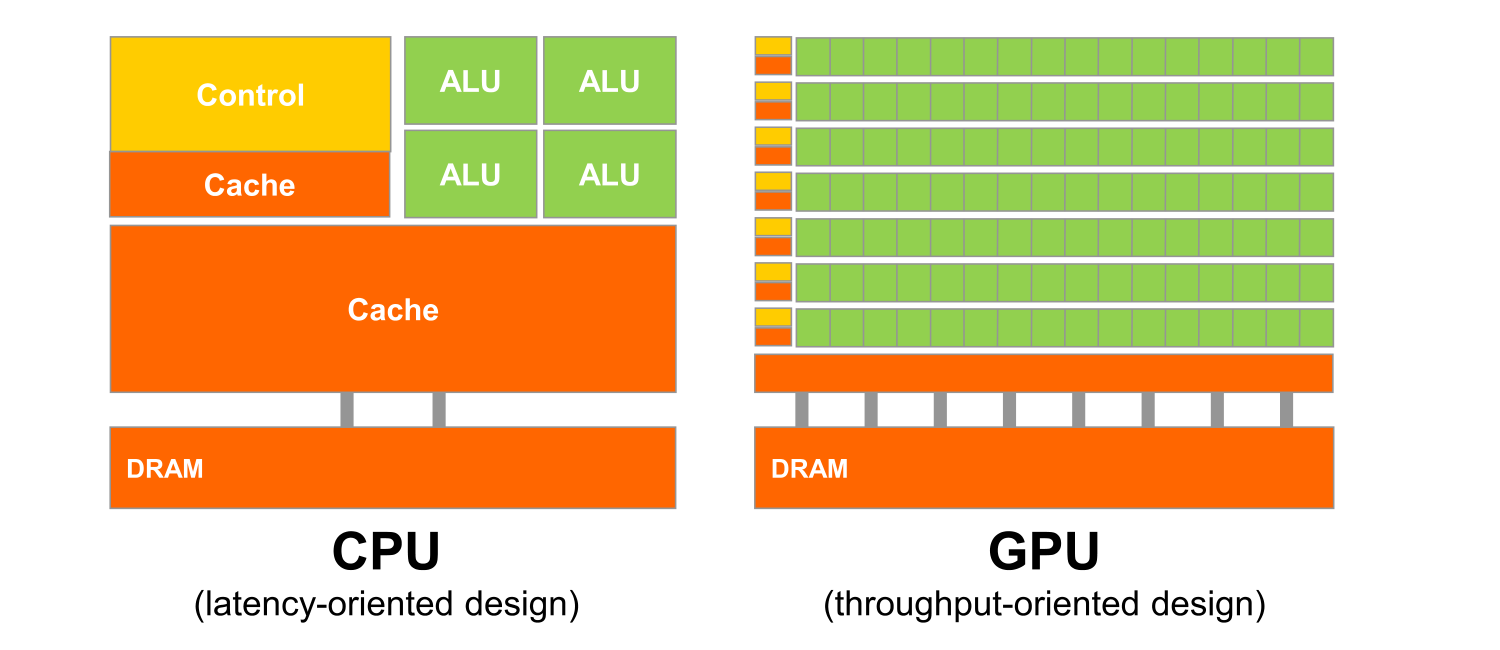
\includegraphics[width=\textwidth]{figs/ch1/1-1.png}
  \caption{CPU 与 GPU 的基本设计理念}
  \label{fig:1-1}
\end{figure}

GPU 应用软件通常需要使用大量并行线程编写。硬件可以利用大量线程，在其中一些
线程等待长延迟内存访问或算术操作时，寻找其他可执行的工作。图 \ref{fig:1-1}
右侧所示的小型缓存用于控制这些应用的带宽需求，使访问相同内存数据的多个线程
不必全部访问 DRAM。这种设计风格通常称为面向吞吐量的设计（throughput-oriented
design）：它允许单个线程可能需要很长时间执行，同时努力最大化大量线程的总体
执行吞吐量。

应当明确，GPU 是为并行、面向吞吐量的计算引擎而设计的；对于 CPU 擅长的某些任务，
GPU 并不会表现良好。对于只有一个或很少线程的程序，具有更低操作延迟的 CPU 可以
获得远高于 GPU 的性能。当程序拥有大量线程时，具有更高执行吞吐量的 GPU 则可以
获得远高于 CPU 的性能。因此，应当预期许多应用会同时使用 CPU 和 GPU：在 CPU
上执行应用的顺序部分，在 GPU 上执行数值密集部分。这正是 NVIDIA 于 2007 年引入
的 CUDA 编程模型被设计用来支持 CPU-GPU 协同执行应用的原因。

应用开发者选择处理器时，速度也不是唯一的决策因素。其他因素甚至可能更加重要。
首先，所选处理器必须在市场上拥有非常广泛的存在，这称为处理器的装机量
（installed base）。原因很简单：只有面对庞大的客户群体，软件开发成本才有充分
的经济合理性。运行在市场占有率很小的处理器上的应用不会拥有广泛的客户群体。
与通用微处理器相比，传统并行计算系统的市场存在极其有限，这一直是一个主要问题。
只有政府和大公司资助的少数精英应用，成功地在这类传统并行计算系统上实现了开发。
众线程 GPU 改变了这一点。由于 GPU 在个人计算机市场上非常流行，其出货量已经达到
数亿。几乎所有台式 PC 和高端笔记本电脑都配有 GPU。如今已有超过 10 亿个支持
CUDA 的 GPU 在使用。如此庞大的市场存在，使这些 GPU 成为对应用开发者具有经济
吸引力的目标。

另一个重要决策因素是实用的形态和易于获得的运行环境。2006 年以前，并行软件应用
主要运行在数据中心服务器或部门级集群上，但这类执行环境往往限制了应用的使用。
例如，在医学成像应用中，基于 64 节点集群机器发表论文没有问题；但实际临床应用
中的 MRI 设备通常由 PC 与专用硬件加速器组合而成。原因很简单：GE 和 Siemens
等制造商不可能向临床场所销售必须配套几机架计算服务器的 MRI 系统，而这样的部署
在高校院系环境中却很常见。事实上，美国国立卫生研究院（NIH）曾有一段时间拒绝
资助并行编程项目，因为他们认为巨型集群机器无法用于临床环境，并行软件的影响会
受到限制。
如今，许多公司已经推出配备 GPU 的 MRI 产品，NIH 也在资助 GPU 计算研究。

在 2006 年以前，图形芯片很难使用，因为程序员必须通过相当于图形 API
（application programming interface，应用程序接口）的函数访问处理单元，也就是
需要使用 OpenGL 或 Direct3D 技术来编程这些芯片。更直白地说，计算必须表达成某种
“绘制像素”的函数，才能在早期 GPU 上执行。这种技术称为 GPGPU，即使用图形处理
器进行通用编程（General Purpose Programming using a Graphics Processing Unit）。
业界更常见的展开是 ``General-Purpose Computing on Graphics Processing Units''；
这里保留原书的表述，并不把两种展开混为一谈。
即使有更高层的编程环境，底层代码仍然需要适配为面向像素绘制的 API。这些 API 限制
了早期 GPU 实际能够编写的应用类型，因此 GPGPU 没有成为普遍的编程现象。尽管如此，
这项技术仍然足够令人兴奋，激励人们完成了一些富有开创性的工作并取得了优秀的研究
成果。

2007 年 CUDA 发布后，一切发生了变化 \cite{cuda2025}。CUDA 带来的并不只是软件变化，
芯片中还增加了额外硬件。NVIDIA 实际上专门划出硅片面积来简化并行编程。在用于并行计算的 G80
及其后继芯片中，GPGPU 程序不再需要经过图形接口，而是由芯片上的新型通用并行
编程接口直接处理 CUDA 程序的请求。这个通用编程接口极大扩展了可以在 GPU 上轻松
开发的应用类型。此外，其他软件层也全部重新设计，使程序员能够使用熟悉的 C/C++
编程工具。

虽然 GPU 是异构并行计算中的重要计算设备类型，但异构计算系统还会把其他重要设备
用作加速器。例如，现场可编程门阵列（field programmable gate array，FPGA）被
广泛用于加速网络应用。本书以 GPU 为学习载体所介绍的技术，同样适用于这类加速器
的编程任务。

\section{为什么需要更高速度或更多并行性？}
\label{sec:why-more-speed}

正如第 \ref{sec:heterogeneous-parallel-computing} 节所述，大规模并行编程的主要
动机，是让应用在未来几代硬件上继续获得速度提升。在“并行模式”和“高级模式与
应用”两部分（第 2、3 部分，即第 7 至第 23 章）中我们会看到，对于适合并行执行
的应用，优秀的 GPU 实现相对于单个 CPU 核心上的顺序执行，可以达到超过
$100\times$ 的加速比。如果应用包含我们所称的“数据并行性”，仅用几个小时的工作
往往就可以获得 $10\times$ 的加速。

有人可能会问，为什么应用会继续要求更高的速度？今天的许多应用似乎已经运行得
足够快了。尽管当今世界有无数计算应用，未来许多令人兴奋的大众市场应用，实际上
就是我们过去称为“超级计算应用”或“超级应用”的东西。

例如，生物学研究界正越来越深入分子层面。显微镜可以说是分子生物学最重要的仪器，
过去主要依靠光学或电子仪器。然而，我们可以借助这些仪器进行的分子级观测存在限制。
把计算模型纳入进来，模拟底层分子活动，并用传统仪器设置边界条件，可以有效地解决
这些限制。借助仿真，我们能够测量比单靠传统仪器所能想象的更多细节，也能检验更多
假设。在可预见的未来，仿真会继续受益于计算速度的提升：在可接受的响应时间内，
能够建模的生物系统规模会扩大，能够模拟的反应时间也会延长。这些增强将对科学和
医学产生巨大影响。

对于视频、音频编码和处理等应用，可以想想我们对数字高清电视（HDTV）相对于旧式
NTSC 电视的满意程度。体验过 HDTV 的细节水平之后，人们很难再回到旧技术。但请
考虑 HDTV 所需的全部处理工作：它是高度并行的过程，三维成像和可视化也一样。未来，
视图合成、把低分辨率视频以高分辨率显示等新功能，将需要电视设备提供更多计算能力。
在消费级产品中，我们正看到越来越多的视频和图像处理应用，用来改善照片和视频的
对焦、光照以及其他关键方面。

更高的计算速度还可以带来更好的用户界面。现代智能手机用户享受着更加自然的交互
界面，高分辨率触摸屏的显示效果足以媲美大屏电视。毫无疑问，未来版本的这类设备
将加入具有三维视角的传感器和显示器、把虚拟空间与物理空间信息结合起来以提高
可用性的应用，以及基于语音和计算机视觉的交互界面；这些功能都需要更高的计算速度。

消费电子游戏中也在发生类似的发展。过去，游戏中的驾驶实际上只是预先安排好的一
组场景：汽车撞上障碍物后，车辆行驶路线并不会改变，只有游戏分数发生变化；车轮
不会弯曲或损坏，无论撞到车轮还是失去一个车轮，驾驶难度都不会改变。随着计算速度
提升，游戏可以基于动态仿真，而不再基于预先安排的场景。未来我们可以体验更多
这样的真实效果：事故会损坏车轮，在线驾驶体验也会逼真得多。准确建模物理现象的
能力已经催生了“数字孪生”概念：物理对象在仿真空间中拥有准确模型，可以以低得多
的成本进行充分的压力测试和劣化预测。对物理效应进行逼真的建模和仿真，通常需要
极其巨大的计算能力。

计算吞吐量大幅提升所带来的新应用中，一个重要例子是基于人工神经网络的深度学习。
尽管神经网络从 20 世纪 70 年代起就一直受到积极研究，但由于训练需要太多带标签
数据和太多计算，它们在实际应用中一度效果不佳。互联网的兴起带来了海量带标签的
图片，GPU 的兴起则带来了计算吞吐量的跃升。结果，自 2012 年以来，基于神经网络
的应用在计算机视觉和自然语言处理领域迅速普及。这种普及彻底改变了计算机视觉和
自然语言处理应用，也推动了自动驾驶汽车和家庭助手设备的快速发展。

上述所有新应用都以不同方式、不同层次模拟和/或表示一个物理的、并发的世界，并且
需要处理极大量数据。面对如此巨大的数据量，大部分计算都可以在数据的不同部分上
并行完成，尽管这些结果最终需要在某个时刻汇合。多数情况下，有效管理数据传送
会对并行应用能够达到的速度产生重大影响。少数每天处理这类应用的专家往往熟悉
相关技术，但绝大多数应用开发者都能从对这些技术更直观的理解和实践性工作知识中
获益。

我们的目标是以直观的方式向应用开发者介绍数据管理技术，而他们的正规教育未必来自
计算机科学或计算机工程。我们还希望提供大量实用代码示例和动手练习，帮助读者
获得真正可工作的知识；这要求有一种既便于并行实现、又支持恰当管理数据传送的
实用编程模型。CUDA 提供了这样的编程模型，并且已经得到庞大开发者社区的充分检验。

\section{加速真实应用}
\label{sec:speeding-up-real-applications}

把应用并行化后，能够期待多大的加速比？计算系统 $A$ 相对于计算系统 $B$ 的应用
加速比，定义为应用在 $B$ 上的执行时间与在 $A$ 上执行同一应用所需时间之比。例如，
某应用在系统 $A$ 上需要 10 秒，在系统 $B$ 上需要 200 秒，那么系统 $A$ 相对于
系统 $B$ 的加速比为
\[
  \frac{200\text{ s}}{10\text{ s}}=20,
\]
即 $20\times$（20 倍）加速。

并行计算系统相对于串行计算系统能够达到的加速比，取决于应用中可以并行化的部分。
例如，如果应用执行时间中可并行部分占 30\%，即使把这部分加速 $100\times$，应用
总执行时间也最多只能减少 29.7\%。换言之，整个应用的加速比只有
\[
  \frac{1}{1-0.297}\approx 1.42\times.
\]
事实上，即使并行部分获得无限大的加速，也只能削减 30\% 的执行时间，最高加速比
不超过约 $1.43\times$。另一方面，如果执行时间的 99\% 都属于并行部分，那么将
并行部分加速 $100\times$ 后，应用执行时间会降至原来的 1.99\%，整个应用可以获得
$50\times$ 加速。因此，要让大规模并行处理器有效加速应用，应用执行时间的绝大
部分必须位于并行部分。并行执行所能达到的加速水平会受到应用可并行部分大小的
严重限制，这一事实称为阿姆达尔定律（Amdahl's Law）\cite{amdahl2013}。

研究人员已经在某些应用上取得超过 $100\times$ 的加速。然而，这通常只有在进行
大量优化和调优之后才可能实现，而且往往还需要改进算法，使应用工作量的
$99.9\%$ 以上处于并行部分。

应用能够达到的加速水平还取决于从内存读取数据以及向内存写入数据的速度。在实践中，
直接对应用进行并行化往往会使内存（DRAM）带宽达到饱和，结果只能获得约
$10\times$ 加速。诀窍在于设法绕过内存带宽限制：通过某种变换利用 GPU 上的专用
片上内存，大幅减少对 DRAM 的访问。不过，代码还需要继续优化，以应对片上内存
容量有限等限制。本书的一个重要目标，就是帮助读者充分理解这些优化方法并熟练
掌握它们。

请记住，相对于单核 CPU 执行所得到的加速水平，也可能反映 CPU 是否适合该应用。
在某些应用中，CPU 的表现非常好，因此很难再用 GPU 提升性能。大多数应用都有
一些部分更适合由 CPU 执行。必须给 CPU 一个公平的机会，并确保代码编写方式能够
让 GPU 与 CPU 执行互补，从而正确利用 CPU/GPU 组合的异构并行计算能力。如今，
结合多核 CPU 和众核 GPU 的大众市场计算系统，已经把万亿次级（terascale）计算
带到了桌面，把百亿亿次级（exascale）计算带到了集群。

图 \ref{fig:1-2} 展示了典型应用的主要组成部分。真实应用的大量代码往往是顺序的。
图中将这些顺序部分画成桃子的“果核区域”：试图对这些部分应用并行计算技术，就像
咬桃核一样——感觉并不好！这些部分很难并行化。CPU 往往能够很好地处理它们。好
消息是，尽管这些部分可能占据大量代码，却往往只占超级应用执行时间的一小部分。

接下来是我们所谓的“桃肉区域”。这些部分容易并行化，早期图形应用也是如此。在
异构计算系统中进行并行编程，可以大幅提升这类应用的速度。如图 \ref{fig:1-2}
所示，早期 GPGPU 编程接口只覆盖桃肉区域的一小部分，这类似于只能覆盖最令人
兴奋的应用中的一小部分。我们将看到，CUDA 编程接口的设计目标是覆盖更多令人
兴奋的应用“桃肉”。并行编程模型及其底层硬件仍在快速演进，以便高效并行化应用中
越来越大的部分。

\begin{figure}[htbp]
  \centering
  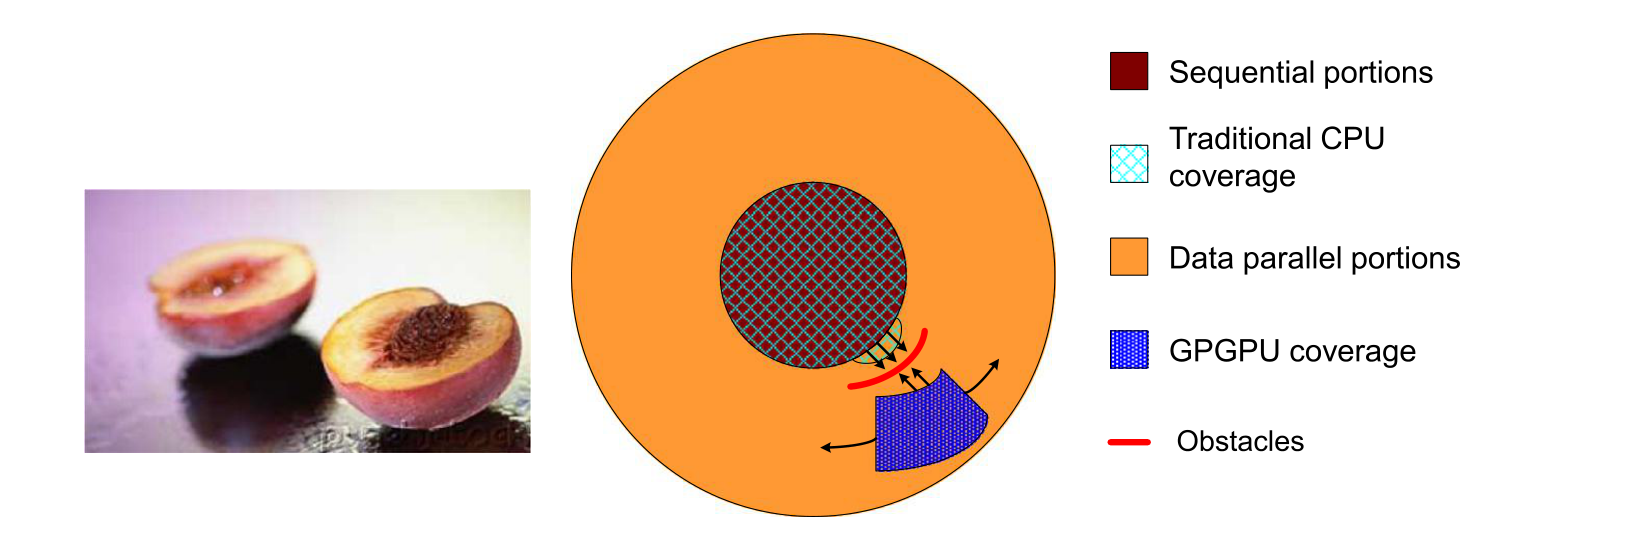
\includegraphics[width=\textwidth]{figs/ch1/1-2.png}
  \caption{顺序部分与数据并行部分的应用结构}
  \label{fig:1-2}
\end{figure}

\section{并行编程中的挑战}
\label{sec:parallel-programming-challenges}

并行编程为什么困难？有人曾说过：如果你不在乎性能，并行编程非常容易；你甚至
可以在一小时内写出并行程序。但如果不在乎性能，又何必编写并行程序呢？

本书讨论如何在并行编程中实现高性能所面临的几个挑战。首先，设计出与顺序算法
具有相同算法（计算）复杂度的并行算法，可能相当困难。许多并行算法与对应的顺序
算法执行相同数量的工作。然而，有些并行算法会做更多工作；事实上，有时它们会
多做如此多工作，以至于在大规模输入数据集上最终运行得更慢。这尤其令人担忧，
因为快速处理大规模输入数据集正是并行编程的重要动机。

例如，许多现实问题最自然的描述方式是数学递推式。把这些问题并行化，通常需要
以反直觉的方式思考问题，执行时也可能需要重复工作。有一些重要的算法原语，例如
前缀和（prefix sum）或扫描（scan），可以帮助我们把问题的顺序递归形式转换为
更适合并行的形式。第 11 章将更正式地介绍工作效率（work efficiency）概念，并
借助前缀和等重要并行模式，说明如何设计具有与对应顺序算法相同计算复杂度的并行
算法，以及其中涉及的方法和权衡。

第二，许多应用的执行速度受内存访问延迟和/或吞吐量限制。我们把这类应用称为
内存受限（memory-bound）应用，以区别于计算受限（compute-bound）应用；后者受
硬件执行算术运算的速率限制。要让内存受限应用实现高性能并行执行，通常需要提高
内存访问速度的方法。第 5 章和第 6 章将介绍内存访问优化技术，并在多章并行模式
与应用中应用这些技术。

第三，相比对应的顺序程序，并行程序的执行速度通常对输入数据特征更加敏感。许多
现实应用必须处理特征变化很大的输入，例如不规则或不可预测的数据规模，以及不
均匀的数据分布。这些规模和分布上的变化，可能导致分配给并行线程的工作量不均，
并显著降低并行执行的有效性。并行程序的性能有时会随这些特征发生剧烈变化。我们
将在介绍并行模式和应用的章节中，介绍使数据分布更加规整，或针对数据特征调整
线程工作分配的技术，以应对这些挑战。

第四，有些应用可以并行化，而且不同线程之间几乎不需要协作。这些应用通常称为
易并行应用（embarrassingly parallel）。另一方面，另一些应用要求线程彼此协作，
这就需要使用屏障或原子操作等同步操作。同步操作会给应用带来开销，因为线程常常
需要等待其他线程，而不是执行有用工作。本书将始终讨论降低这种同步开销的各种
策略。

幸运的是，研究人员过去已经解决了其中许多挑战。不同应用领域之间还存在共同模式，
使我们能够把一个领域中得到的解决方案应用到其他领域。这正是本书选择在重要并行
计算模式和应用的语境中介绍应对这些挑战的关键技术的主要原因。

\section{相关并行编程接口}
\label{sec:related-parallel-interfaces}

过去几十年间，人们已经开发出许多并行编程语言和模型
\cite{mattson2004}。应用最广泛的包括：用于共享内存多处理器系统的 OpenMP
\cite{openmp2025}，以及用于可扩展集群计算的消息传递接口（Message Passing
Interface，MPI）\cite{mpi1994}。二者都已经成为由主要计算机厂商支持的标准化
编程接口。

一个 OpenMP 实现由编译器和运行时系统组成。程序员向 OpenMP 编译器指定有关循环
的指令（directive）和编译提示（pragma）。借助这些指令和提示，OpenMP 编译器
生成并行代码。运行时系统通过管理并行线程和资源，支持并行代码的执行。OpenMP
最初为 CPU 执行设计，后来扩展到支持 GPU 执行。OpenMP 的主要优点是，它提供
编译器自动化和运行时支持，从而把许多并行编程细节抽象掉。这样的自动化和抽象，
有助于让应用代码在不同厂商生产的系统之间，以及同一厂商不同代际的系统之间，
实现更好的可移植性。我们把这一性质称为性能可移植性（performance portability）。
不过，要有效地使用 OpenMP，程序员仍然需要理解涉及的全部并行编程概念。由于
CUDA 让程序员能够显式控制这些并行编程细节，因此即使读者打算把 OpenMP 作为
主要编程接口，CUDA 也是很好的学习载体。此外，根据我们的经验，OpenMP 编译器
仍在不断发展和改进。许多程序员可能仍需在 OpenMP 编译器能力不足的部分使用
CUDA 风格的接口。

MPI 是一种编程接口：集群中的计算节点不共享内存，所有数据共享和交互都必须通过
显式消息传递完成。MPI 已广泛用于高性能计算（high-performance computing，HPC）。
使用 MPI 编写的应用已经在超过 100,000 个节点的集群计算系统上成功运行。如今，
许多 HPC 集群采用异构 CPU/GPU 节点。由于计算节点之间没有共享内存，把应用移植
到 MPI 可能需要相当大的工作量。程序员需要进行域分解，把输入和输出数据划分到
各个节点上；还需要根据域分解结果调用消息发送和接收函数，管理节点之间的数据
交换。

另一方面，CUDA 为 GPU 内部的并行执行提供了共享内存，可以解决这一困难。CUDA
适合节点内部的编程，但大多数应用开发者仍需要使用 MPI 一类的接口来编程集群
层级。随着 MPI 本身逐渐具备 CUDA 感知能力，以及 NCCL 和 NVSHMEM 等其他 API
不断提供支持，CUDA 的多 GPU 编程能力也在增强。因此，在使用多 GPU 节点的现代
计算集群中，并行程序员必须理解如何在 MPI 等多 GPU 编程模型的语境下进行 CUDA
编程；第 23 章将介绍这一内容。

2009 年，包括 Apple、Intel、AMD/ATI 和 NVIDIA 在内的多个产业参与者共同开发了
一种标准化编程模型，称为开放计算语言（Open Computing Language，OpenCL）
\cite{opencl2008}。原书正文将其写作 ``Open Compute Language''；译文采用 OpenCL
的官方展开。与 CUDA 类似，OpenCL 编程模型定义了语言扩展和运行时 API，
允许程序员管理大规模并行处理器中的并行性和数据传送。与 CUDA 相比，OpenCL
更多依赖 API，而较少依赖语言扩展。这样，厂商就可以快速调整现有编译器和工具，
以处理 OpenCL 程序。

OpenCL 是一种标准化编程模型：使用 OpenCL 开发的应用，无需修改，就能在所有
支持 OpenCL 语言扩展和 API 的处理器上正确运行。不过，要在新的处理器上获得
高性能，通常仍然需要修改应用。熟悉 OpenCL 和 CUDA 的读者会知道，二者的关键
概念和特性非常相似。也就是说，CUDA 程序员只需很少努力就能学会 OpenCL 编程。
更重要的是，使用 CUDA 学到的几乎所有技术，都可以轻松应用于 OpenCL 编程。

\section{总体目标}
\label{sec:overarching-goals}

我们的首要目标是教会读者如何编程大规模并行处理器，以实现高性能。因此，本书
很大一部分内容都致力于开发高性能并行代码的技术。我们的方法不要求读者具备
大量硬件专业知识；不过，读者需要对并行硬件架构有良好的概念性理解，才能推理
代码的性能行为。因此，我们会用一些篇幅帮助读者直观理解基本硬件架构特征，并用
大量篇幅介绍开发高性能并行程序的技术。特别是，我们将重点讨论计算思维
（computational thinking）\cite{wing2006} 技术，使读者能够用适合在大规模并行
处理器上高性能执行的方式思考问题。

在大多数处理器上进行高性能并行编程，都需要了解硬件的工作方式。要构建工具和
机器，使程序员不必了解这些知识就能开发高性能代码，可能还需要很多年。即使有了
这样的工具，我们也怀疑了解硬件的程序员会比不了解硬件的人更有效地使用它们。
因此，第 4 章将介绍 GPU 架构的基础；在讨论高性能并行编程技术时，我们还会讨论
更加专门的架构概念。

我们的第二个目标是教授如何编写功能正确且可靠的并行程序；这是并行计算中
一个微妙的问题。曾经开发过并行系统的人都知道，实现初始性能还不够，真正的挑战
是以一种能够调试代码并支持用户的方式实现性能。CUDA 编程模型鼓励使用简单形式
的屏障同步、原子性和内存一致性来管理并行性。此外，它还提供了一组强大的工具，
不仅可以调试功能问题，也可以定位性能瓶颈。

我们的第三个目标是让程序能够跨越未来的硬件代际进行扩展：探索并行编程方法，使
未来更加并行的机器能够比今天的机器更快地运行代码。我们希望帮助读者掌握并行
编程，使程序能够扩展到新一代机器的性能水平。实现这种可扩展性的关键，是使内存
数据访问更加规整和局部化，从而尽量减少关键资源的消耗以及更新数据结构时发生的
冲突。因此，开发高性能并行代码的技术，对保证应用在未来的可扩展性同样重要。

要实现这些目标，需要大量技术知识，因此本书会介绍不少并行编程原则和模式
\cite{mattson2004}。我们不会孤立地教授这些原则和模式，而是把它们放在有用应用
的并行化语境中来讲授。当然，我们无法覆盖全部原则和模式，所以选择了最有用且
经过充分验证的技术进行详细介绍。事实上，本版显著增加了关于并行模式和应用的
章节。现在，让我们快速概览本书其余内容。

\section{本书的组织结构}
\label{sec:book-organization}

本书分为三部分。第 1 部分介绍并行编程、数据并行、GPU 以及性能优化的基本概念。
这些基础章节为读者成为 GPU 程序员提供必要的知识和技能。第 2 部分介绍基本的
并行模式，第 3 部分介绍更高级的并行模式和应用。这两部分会应用第一部分所学的
知识和技能，也会在需要时引入其他 GPU 架构特性和优化技术。

第 1 部分“基础概念”包括第 2 至第 6 章。第 2 章介绍数据并行和 CUDA 编程模型，
并假设读者此前有 C++ 编程经验。它首先把 CUDA 介绍为 C++ 的一个简单而小型的
扩展，用于支持异构 CPU/GPU 计算以及广泛使用的单程序多数据（Single Program
Multiple Data，SPMD）并行编程模型。随后，本章介绍以下思考过程：

\begin{enumerate}
  \item 识别应用程序中需要并行化的部分；
  \item 隔离并行代码将使用的数据，并通过 API 函数在并行计算设备上分配内存；
  \item 通过 API 函数把数据传送到并行计算设备；
  \item 把并行部分开发为由并行线程执行的内核函数；
  \item 启动内核函数，让并行线程执行它；
  \item 最终通过 API 函数调用把数据传回主机处理器。
\end{enumerate}

我们使用向量加法这一贯穿示例来说明这些概念。第 2 章的目标，是让读者掌握足够
的 CUDA 编程模型概念，以便编写简单的并行 CUDA 程序；同时，它也涵盖了基于任何
并行编程接口开发并行应用所需的若干基本技能。

第 3 章进一步介绍 CUDA 的并行执行模型，尤其是它如何处理多维数据以及多维线程
组织方式。本章提供关于线程创建、组织、资源绑定和数据绑定的足够洞见，使读者
能够使用 CUDA 实现复杂计算。

第 4 章介绍 GPU 计算架构，重点讨论计算核心如何组织，以及线程如何被调度到这些
核心上执行。本章还讨论各种架构因素及其对 GPU 上运行代码性能的影响，包括透明
可扩展性、SIMD 执行与控制分歧、多线程与延迟容忍度，以及占用率（occupancy）
等概念。

第 5 章在第 4 章基础上讨论 GPU 的内存架构，以及可用于保存 CUDA 变量、管理数据
传送和提高程序执行速度的特殊内存。本章介绍分配和使用这些内存的 CUDA 语言特性。
恰当地使用这些内存，可以大幅提高数据访问吞吐量，并帮助缓解内存系统中的流量
拥塞。

第 6 章介绍当前 CUDA 硬件中的若干重要性能因素，尤其是理想的线程执行模式和
内存访问模式。这些细节构成了程序员推理计算和数据组织决策后果的概念基础。本章
最后给出 GPU 程序员经常使用的常见优化策略检查清单，用于优化各种计算模式。
在本书接下来的两部分中，我们会反复使用这份检查清单来优化不同的并行模式和应用。

第 2 部分“基本并行模式”包括第 7 至第 15 章。第 7 章介绍卷积，这是一种常用的
并行计算模式，源于数字信号处理和计算机视觉，并且需要仔细管理数据访问局部性。
我们还借助该模式介绍现代 GPU 中的常量内存和缓存。第 8 章介绍与卷积相似的
模板计算，但它源于求解微分方程，并具有为数据访问局部性进一步优化提供独特机会
的特征。本章还用来介绍线程与数据的三维组织，并展示第 6 章中针对线程粒度的优化
方法。

第 9 章讨论直方图，这是一种广泛用于统计数据分析和大规模数据集模式识别的模式。
我们还借助该模式介绍原子操作，用于协调对共享数据的并发更新；并介绍私有化
（privatization）优化，以降低这些操作的开销。第 10 章介绍归约树模式，用于概括
一组输入数据；同时用它展示控制分歧和过多屏障同步对性能的影响，以及减轻这些影响
的技术。第 11 章介绍前缀和或扫描，这是一种重要的并行计算模式，可以把本质上
顺序的计算转换为并行计算；我们也借此介绍并行算法中的工作效率概念。第 12 章
以两种形式介绍过滤模式：不稳定过滤（允许改变被过滤元素的原始顺序）和稳定过滤
（必须保留原始顺序）。不稳定过滤用于展示线程如何协作以减少原子操作，稳定过滤
则展示第 11 章介绍的扫描模式的一个重要应用。第 13 章介绍并行归并，这是分治式
工作划分策略中广泛使用的模式；本章还介绍动态输入数据识别与组织。最后，第
14 章介绍 GPU 上的排序，涵盖三种并行排序算法：奇偶排序、归并排序（依赖第 13
章的归并模式）以及基数排序（依赖第 11 章介绍的扫描模式）。第 15 章更深入地
重新讨论矩阵乘法，应用第 6 章检查清单中的大量高级优化方法。

\footnote{原书此处把基数排序所依赖的扫描模式标为 Chapter 14；按本书目录和上下文，
应为 Chapter 11。译文按语境更正，并保留此译者注。}

第 3 部分“高级并行模式与应用”在精神上与第 2 部分类似，但所涵盖的模式更加复杂，
通常也包含更多应用背景。因此，这些章节较少侧重介绍新技术或新特性，而更多关注
特定应用的考量。对于每个应用，我们首先识别构造并行执行的不同方式，然后分析
每种方式的优点和缺点，接着逐步进行实现高性能所需的代码变换。这些章节帮助读者
把前面章节的全部材料结合起来，并为读者承担自己的应用开发项目提供支持。

第 3 部分包括第 16 至第 23 章。第 16 章以图处理中的经典 Floyd--Warshall 算法
和基因组序列比对中的 Smith--Waterman 算法为贯穿示例，展示动态规划和波前并行。
第 17 章介绍稀疏矩阵计算，这一技术广泛用于处理极大规模数据集。本章向读者介绍
重新排列数据以实现更高效并行访问的概念，包括数据压缩、填充、排序、转置和规整化。
第 18 章介绍图算法，以及如何在 GPU 编程中高效实现图搜索。本章给出并行化图算法
的多种策略，并讨论图结构如何影响最佳算法的选择；这些策略建立在直方图和归并等
更基本的模式之上。

第 19 章和第 20 章讨论深度学习，它已经成为 GPU 计算中极其重要的领域。第 19 章
介绍卷积神经网络的高效实现，利用分块等技术和卷积等模式。第 20 章介绍大语言
模型，并讨论在 GPU 上训练和推理这些模型的先进优化方法，例如 KV 缓存和批处理。
第 21 章讨论静电势图计算，以及如何利用从散布到聚集的变换来增强并行性、降低
同步开销。

第 22 章介绍计算思维，即以更适合高性能计算的方式构造和求解计算问题的艺术。
本章讨论如何组织程序的计算任务，使其能够并行执行。我们首先讨论把抽象的、特定
于科学问题的概念转化为计算任务的过程；无论开发串行还是并行应用，这是生成高质量
应用软件的重要第一步。随后，我们讨论并行算法结构及其对应用性能的影响，并以
CUDA 性能调优经验为基础。虽然我们不深入介绍这些并行编程风格的实现细节，但希望
读者能够凭借本书打下的基础，学会使用其中任何一种风格编程。本章最后区分并行化
计算的两种广泛策略：以输入为中心和以输出为中心，并回到书中介绍的模式与应用，
回顾性地研究每种模式和应用所采用的策略。

第 3 部分的最后一章，即第 23 章，介绍异构集群上的 CUDA 编程，其中每个计算节点
都包含 CPU 和 GPU。我们讨论如何在 CUDA 的配合下使用 MPI、NCCL 和 NVSHMEM
三种不同编程模型，把计算分配到集群中的多个 GPU，同时降低通信开销。

虽然本书各章都以 CUDA 为基础，但它们帮助读者建立的是一般并行编程的基础。我们
相信，人类从具体示例中学习效果最好：也就是说，必须首先在某个特定编程模型的
语境中学习概念；该模型为我们把知识推广到其他编程模型提供坚实立足点。在推广
过程中，我们可以借助从 CUDA 示例中获得的具体经验。深入体验 CUDA 也能帮助我们
形成成熟的理解，从而学习那些甚至可能与 CUDA 模型无关的概念。

第 24 章将对大规模并行编程作总结并展望未来。我们首先重新审视本书目标，总结各章
如何共同帮助实现这些目标；然后预测快速发展的大规模并行计算会使其成为未来十年
最令人兴奋的领域之一。

\begin{chapterbibliography}{10}

\bibitem{vonneumann1993}
J. von Neumann.
First draft of a report on the EDVAC.
\emph{IEEE Annals of the History of Computing}, 15(4), 1993, 27--75.

\bibitem{sutter2005}
H. Sutter and J. Larus.
Software and the concurrency revolution: leveraging the full power of multicore
processors demands new tools and new thinking from the software industry.
\emph{ACM Queue}, 3(7), 2005, 54--62.

\bibitem{hwu2008}
W.-M. Hwu, K. Keutzer, and T. G. Mattson.
The concurrency challenge.
\emph{IEEE Design \& Test of Computers}, 25(4), 2008, 312--320.

\bibitem{cuda2025}
NVIDIA.
\emph{CUDA C++ Programming Guide}, Release 13.0, 2025.
\url{https://docs.nvidia.com/cuda/cuda-c-programming-guide}.

\bibitem{amdahl2013}
G. M. Amdahl.
Computer architecture and Amdahl's law.
\emph{Computer}, 46(12), 2013, 38--46.

\bibitem{mattson2004}
T. G. Mattson, B. Sanders, and B. Massingill.
\emph{Patterns for Parallel Programming}.
Pearson Education, 2004.

\bibitem{openmp2025}
OpenMP.org.
\emph{OpenMP: The OpenMP API Specification for Parallel Programming}, 2025.
\url{https://www.openmp.org}.

\bibitem{mpi1994}
MPI Forum.
\emph{MPI: A Message-Passing Interface Standard}, 1994.

\bibitem{opencl2008}
Khronos OpenCL Working Group.
\emph{The OpenCL Specification}, Version 1.0, 2008.

\bibitem{wing2006}
J. M. Wing.
Computational thinking.
\emph{Communications of the ACM}, 49(3), 2006, 33--35.

\end{chapterbibliography}


\part{基础概念}
\chapter{异构数据并行计算}
\label{chap:heterogeneous-data-parallel-computing}

数据并行性是这样一种现象：要在数据集的不同部分上执行的计算彼此独立，因此
可以并行执行。许多应用都具有丰富的数据并行性，适合进行可扩展的并行执行；在
这种执行方式下，执行速度会随着系统中执行资源数量的增加而近似成比例地提高。
因此，并行程序员有必要熟悉数据并行性的概念，以及用于编写能够利用数据并行性的
代码的并行编程语言构造。本章将使用 CUDA C++ 语言构造开发一个简单的数据并行
程序。

\section{数据并行性}
\label{sec:data-parallelism}

现代软件应用运行缓慢时，问题通常来自数据——需要处理的数据太多。图像处理应用
会处理包含数百万乃至数万亿像素的图像或视频；科学应用会用数十亿个网格点模拟
流体动力学；分子动力学应用会模拟数千到数十亿个原子之间的相互作用；航空公司
排班则必须处理数千个航班、机组和机场登机口。通常，这些像素、粒子、网格点、
相互作用、航班等对象在很大程度上可以独立处理。

例如，在图像处理中，把彩色像素转换为灰度只需要该像素的数据；模糊图像时，把
每个像素的颜色与附近像素的颜色求平均，只需要一个很小的像素邻域。即使是看起来
需要全局信息的操作，例如求图像中所有像素的平均亮度，也可以拆分成许多能够独立
执行的较小计算。对不同数据片段进行这种相互独立的求值，就是数据并行性的基础。
编写数据并行代码，意味着围绕数据重新组织计算，使得到的独立计算能够并行执行，
从而更快——通常是快得多——地完成整体任务。

下面用一个彩色图像转灰度图像的例子说明数据并行性。图 \ref{fig:2-1} 中的左图
是由许多像素组成的彩色图像，每个像素包含红、绿、蓝三个分数值 $(r,g,b)$，取值
从 0（黑色）到 1（最大强度）。要把彩色图像转换为灰度图像，需要对每个像素
应用下面的加权和公式，计算亮度值 $L$：
\[
  L = r \times 0.299 + g \times 0.587 + b \times 0.114.
  \tag{2.1}
\]

\begin{figure}[htbp]
  \centering
  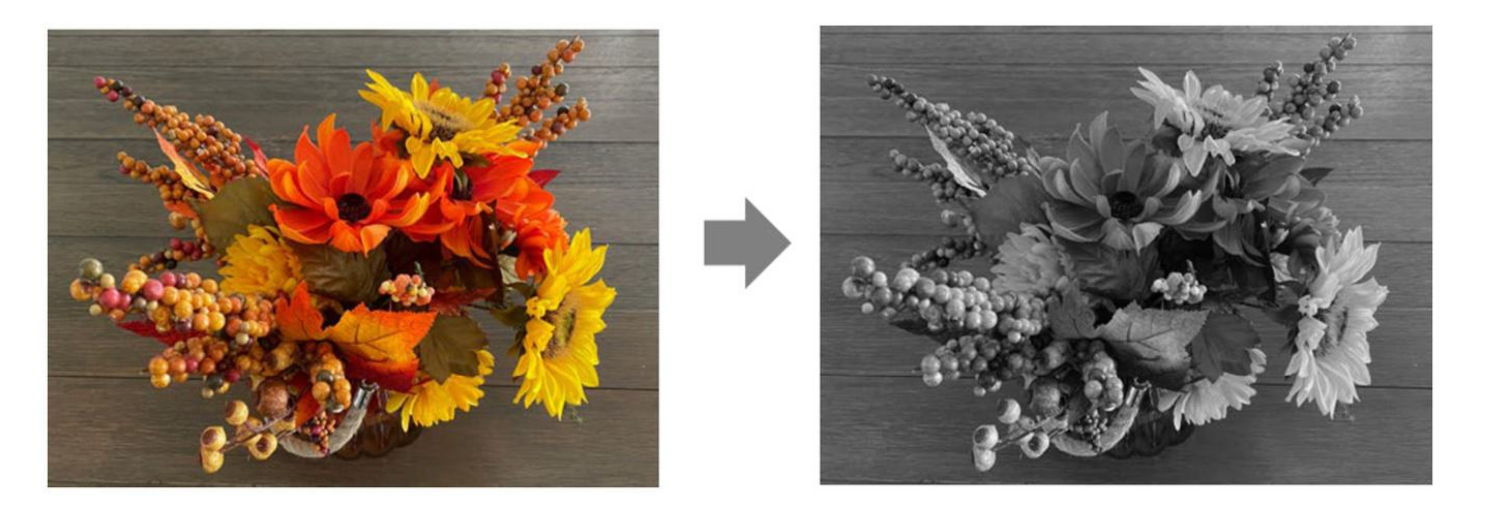
\includegraphics[width=\textwidth]{figs/ch2/2-1.png}
  \caption{彩色图像转换为灰度图像}
  \label{fig:2-1}
\end{figure}

\begin{quote}
\textbf{RGB 彩色图像表示}

在 RGB 表示中，图像的每个像素都表示为一个 $(r,g,b)$ 值元组。一行图像的格式
可以写成$(r\ g\ b)\ (r\ g\ b)\ \cdots\ (r\ g\ b)$.每个元组表示红光（R）、绿光（G）和蓝光（B）的混合。
也就是说，渲染像素时，每个像素的 $r$、$g$ 和 $b$ 值分别表示红、绿、蓝光源的强度，其中 0 表示暗，1 表示满强度。
\begin{center}
  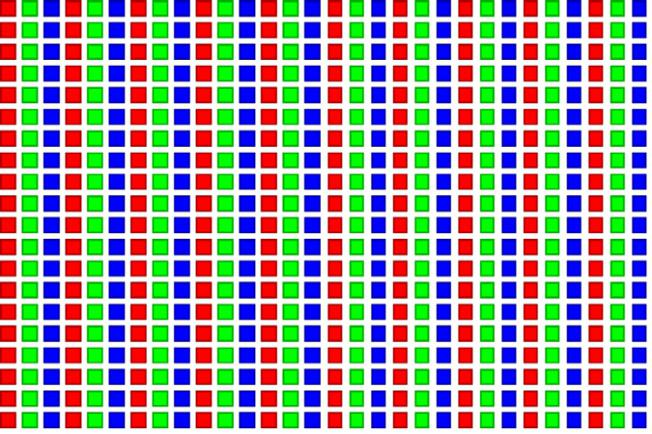
\includegraphics[width=0.5\textwidth]{figs/ch2/RGB.png}
\end{center}

\end{quote}

如果把输入看作由 RGB 值组成的数组 $I$，把输出看作对应的亮度值数组 $O$，就能
得到图 \ref{fig:2-2} 所示的简单计算结构。例如，$O[0]$ 是按照上面的公式对
$I[0]$ 中的 RGB 值求加权和得到的；$O[1]$ 由 $I[1]$ 中的 RGB 值得到；$O[2]$
由 $I[2]$ 中的 RGB 值得到，以此类推。这些逐像素计算彼此没有依赖，全部可以独立
执行。显然，彩色转灰度体现了丰富的数据并行性，因为现代图像通常包含数百万个
像素。当然，完整应用中的数据并行性可能更加复杂；本书很大一部分内容都致力于
教授发现并利用数据并行性所需的“并行思维”。

\begin{figure}[htbp]
  \centering
  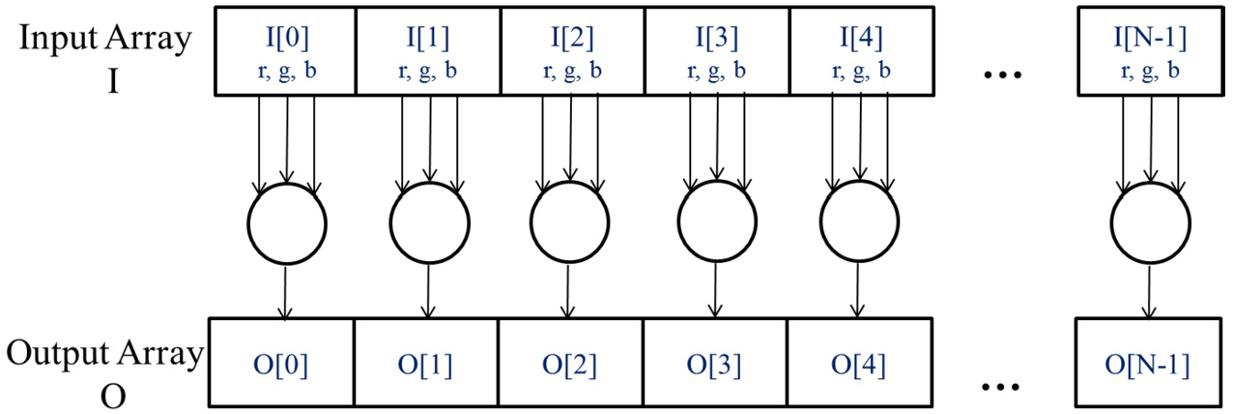
\includegraphics[width=\textwidth]{figs/ch2/2-2.png}
  \caption{彩色转灰度中的数据并行性：像素可以独立计算}
  \label{fig:2-2}
\end{figure}

\begin{quote}
\textbf{数据并行性与任务并行性}

数据并行性并不是并行编程中唯一使用的并行性类型。任务并行性也被广泛用于并行
编程。任务并行性通常通过对应用进行任务分解来暴露。例如，一个简单应用可能需要
执行向量加法和矩阵--向量乘法；这两项工作各自就是一个任务。如果两个任务可以
独立执行，就存在任务并行性。I/O 和数据传送也是常见的任务来源。

大型应用通常包含更多相互独立的任务，因此具有更多任务并行性。例如，在分子动力学
模拟器中，自然任务可能包括振动力计算、转动力计算、非键合力的邻居识别、非键合
力计算，以及速度和位置计算等。
\end{quote}

一般而言，数据并行性是并行程序获得性能提升的主要来源。面对大规模数据集，通常
可以找到充足的数据并行性，从而利用大规模并行处理器，并让应用性能随着每一代
拥有更多执行资源的硬件而提升；这种理想性质称为可扩展性（scalability）。不过，
任务并行性同样可能在实现性能目标时发挥重要作用。

\section{CUDA C++ 程序结构}
\label{sec:cuda-cpp-program-structure}

下一步是学习如何编写程序，在异构计算系统中利用数据并行性以获得更快的执行速度。
为了一般性地说明本书中的算法和技术，我们将使用 CUDA C++ 程序的代码示例。根据
我们的经验，基于 CUDA C++ 学到的概念很容易扩展到其他编程语言和平台。

CUDA C++\footnote{本书的代码示例为简洁起见使用 C 风格编程，并在需要时介绍 C++
特性。不过，读者应当注意，CUDA 编程已经逐渐转向 C++，以支持现代泛型编程和其他
面向对象的编程实践。} 在流行的 C++ 编程语言基础上，以少量新语法和库函数扩展
出面向异构计算系统的能力，使程序员能够针对同时包含 CPU 和 GPU 的系统编程。
顾名思义，CUDA C++ 建立在 NVIDIA 的 CUDA 平台之上。CUDA 目前是大规模并行
计算中最成熟的框架，已广泛用于高性能计算产业；在最常见的操作系统上，都能找到
编译器、调试器和性能分析器等重要工具。

CUDA C++ 程序的结构反映了计算机中主机（host，即 CPU）与一个或多个设备（device，
即 GPU）共存的情况。每个 CUDA C++ 源文件都可以混合包含主机代码和设备代码。
默认情况下，任何只包含主机代码的传统 C++ 程序也是一个 CUDA C++ 程序；可以在
任意源文件中加入设备代码。设备代码由特殊的 CUDA C++ 关键字明确标记，其中包括
函数（或称内核，kernel），其代码以数据并行方式执行。

图 \ref{fig:2-3} 展示了 CUDA C++ 程序的执行过程。执行从主机代码（CPU 串行代码）
开始，图中用一条代表线程的弯曲箭头表示。当调用内核——也就是设备代码的一部分
（图中的设备并行内核）——时，设备上会启动大量线程执行该内核。一次内核调用
所启动的全部线程统称为一个网格（grid）。这些线程是 CUDA 平台中并行执行的主要
载体。图 \ref{fig:2-3} 展示了两个线程网格的执行，每个网格又由多个线程块组成；
稍后会讨论网格和线程块的组织方式。当网格中的所有线程执行完毕后，网格终止，
执行回到主机，直到再次启动另一个网格。正如图中所暗示的，异构计算应用可以管理
CPU 和 GPU 的重叠执行，从而同时利用二者。

\begin{figure}[htbp]
  \centering
  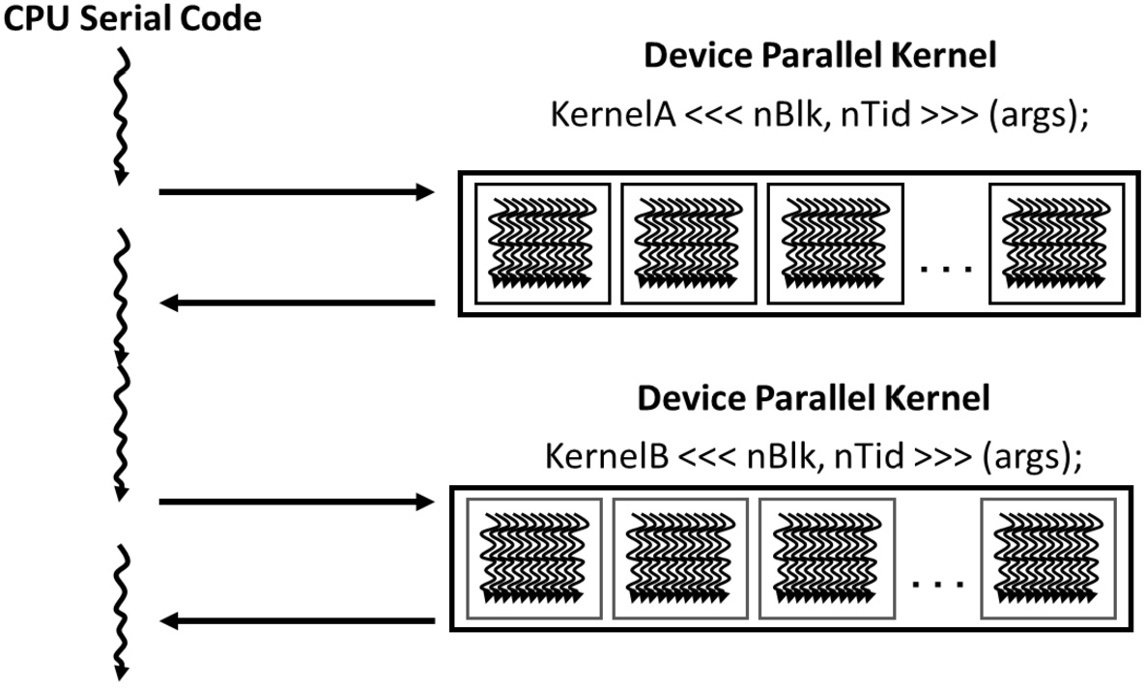
\includegraphics[width=\textwidth]{figs/ch2/2-3.png}
  \caption{CUDA 程序的执行过程}
  \label{fig:2-3}
\end{figure}

\begin{quote}
\textbf{线程}

线程是现代计算机中处理器执行顺序程序方式的一种简化视图。线程由程序代码、
当前正在执行的代码位置，以及变量和数据结构的值组成。从用户角度看，线程的执行
是顺序的。程序员可以使用源代码级调试器，逐条执行语句来监控线程进展，查看下一条
将要执行的语句，并在执行推进时检查变量和数据结构的值。

线程已经在编程中使用多年。如果程序员希望在应用中启动并行执行，就可以借助线程
库或专用语言创建并管理多个线程。在 CUDA 中，每个设备线程的执行同样是顺序的；
CUDA 程序通过调用内核函数启动并行执行，底层运行时机制则负责在设备上启动一个
线程网格，让线程并行处理数据。
\end{quote}

启动一个网格通常会生成大量线程，以利用数据并行性。在彩色转灰度的例子中，可以
让每个线程计算输出数组中的一个像素；此时，网格启动所生成的线程数应等于图像中
像素的数量。对于大图像，可能会生成数百万个线程。实践中，也可以让每个线程计算
多个输出像素，以提高执行和数据访问效率；本书后文会讨论这一点。由于硬件支持
高效的线程生成和调度，CUDA 程序员可以假设这些线程只需很少的时钟周期就能生成
和调度；传统 CPU 线程的生成和调度通常则需要数千个时钟周期。第 3 章将展示如何
实现彩色转灰度和图像模糊\textcolor{red}{内核}，本章为简洁起见使用向量加法作为贯穿示例。

\section{向量加法示例}
\label{sec:vector-addition-example}

向量加法可以说是最简单的数据并行计算，\textcolor{red}{是顺序编程中 ``Hello World'' 的并行
对应物}。在展示向量加法的内核代码之前，先回顾传统向量加法（主机代码）函数的
工作方式会很有帮助。图 \ref{fig:2-4} 展示了一个由 \code{main} 函数和向量加法
函数组成的简单 C++ 程序。

在本书的所有示例中，只要需要区分主机数据和设备数据，就会在主机使用的变量名
后加上 \code{_h}，在设备使用的变量名后加上 \code{_d}，以提醒自己这些变量的
预期用途。由于图 \ref{fig:2-4} 只有主机代码，因此其中只出现带 \code{_h} 后缀
的变量。

假设要相加的向量存放在数组 $A$ 和 $B$ 中，它们在 \code{main} 函数中分配并初始化；
输出向量存放在数组 $C$ 中，该数组也在 \code{main} 函数中分配。为简洁起见，图中
没有展示 \code{main} 函数如何分配和初始化 $A$、$B$、$C$ 的细节。这些数组的
指针，以及表示向量长度的变量 $N$，会传给 \code{vecAdd} 函数。注意，
\code{vecAdd} 的参数带有 \code{_h} 后缀，以强调它们由主机使用。

\begin{figure}[htbp]
  \centering
  \begin{lstlisting}[language=C++]
// Compute vector sum C_h = A_h + B_h
void vecAdd(float* A_h, float* B_h, float* C_h, int n) {
    for (int i = 0; i < n; ++i) {
        C_h[i] = A_h[i] + B_h[i];
    }
}
int main() {
    // Memory allocation for arrays A, B, and C
    // I/O to read A, B, and N elements each
    ...
    vecAdd(A, B, C, N);
}
  \end{lstlisting}
  \caption{一个简单的传统向量加法 C++ 代码示例}
  \label{fig:2-4}
\end{figure}

\begin{quote}
\textbf{C++ 语言中的指针}

图 \ref{fig:2-4} 中的函数参数 $A$、$B$、$C$ 都是指针。在 C 和 C++ 语言中，可以
使用指针访问变量和数据结构。浮点变量 $V$ 可以声明为：
\[
\code{float V;}
\]
指针变量 $P$ 可以声明为：
\[
\code{float *P;}
\]
通过语句 \code{P = &V} 把 $V$ 的地址赋给 $P$，就可以让 $P$“指向”$V$。
\code{*P} 成为 $V$ 的同义表示。例如，\code{U = *P} 把 $V$ 的值赋给 $U$；
又如，\code{*P = 3} 会把 $V$ 的值改为 3。

C 或 C++ 程序中的数组可以通过指向其第 0 个元素的指针访问。例如，语句
\code{P = &(A[0])} 让 $P$ 指向数组 $A$ 的第 0 个元素，于是 \code{P[i]} 就
成为 \code{A[i]} 的同义表示。事实上，数组名 $A$ 本身就是指向其第 0 个元素的
指针。
\end{quote}

在图 \ref{fig:2-4} 中，调用 \code{vecAdd} 时把数组名 $A$ 作为第一个参数，会让
函数的第一个参数 \code{A_h} 指向 $A$ 的第 0 个元素。因此，函数体中的
\code{A_h[i]} 可以用来访问 \code{main} 函数中定义的数组 $A$ 的 \code{A[i]}。
关于 C 语言中指针详细用法的易读解释，可参见文献 \cite{patt2020}。

\code{vecAdd} 函数使用 \code{for} 循环遍历向量元素。在第 $i$ 次迭代中，输出
元素 \code{C_h[i]} 接收 \code{A_h[i]} 和 \code{B_h[i]} 的和。向量长度参数
\code{n} 用于控制循环，使迭代次数与向量长度相匹配。函数分别通过指针
\code{A_h}、\code{B_h} 和 \code{C_h} 读取 $A$、$B$ 的元素并写入 $C$ 的元素。
\code{vecAdd} 返回后，\code{main} 中的后续语句就可以访问 $C$ 的新内容。

在并行执行向量加法的一种直接方法，是修改 \code{vecAdd} 函数，把计算移到设备上。
这种修改后的 \code{vecAdd} 函数结构如图 \ref{fig:2-5} 所示。函数的第 1 部分
在设备（GPU）内存中分配空间，保存 $A$、$B$、$C$ 向量的副本，并把 $A$ 和 $B$
向量从主机内存复制到设备内存。第 2 部分调用向量加法内核，在设备上启动一个
线程网格。第 3 部分把和向量 $C$ 从设备内存复制到主机内存，并释放设备内存中的
三个数组。

\begin{figure}[htbp]
  \centering
  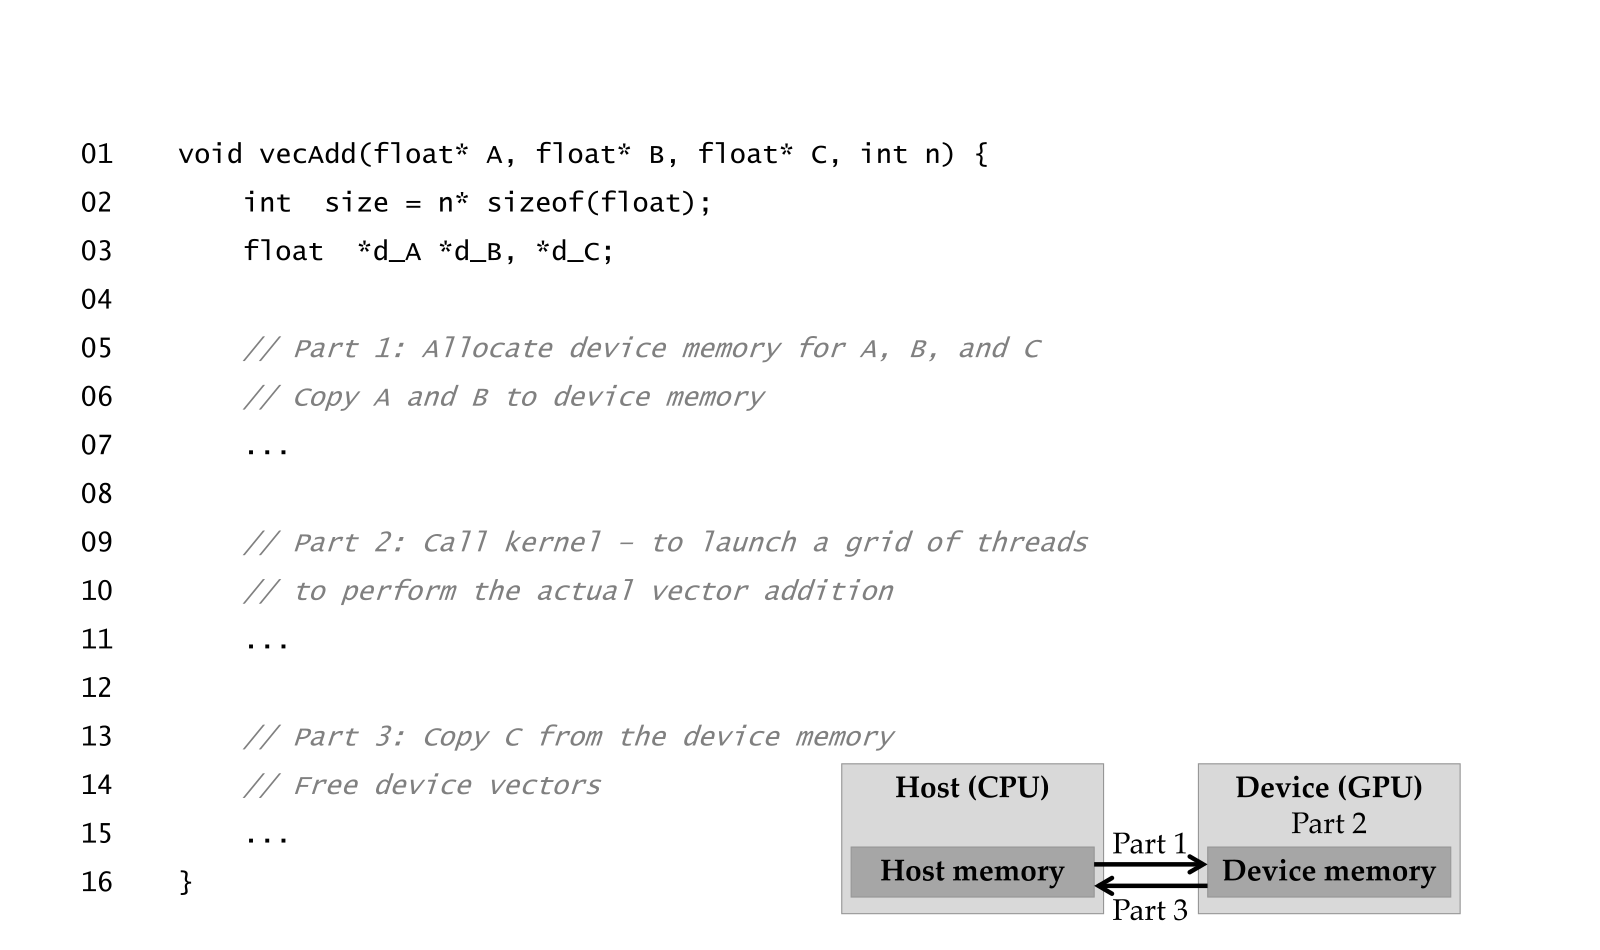
\includegraphics[width=\textwidth]{figs/ch2/2-5.png}
  \caption{把工作移到设备上的 \code{vecAdd}（主机代码）函数概要及数据流}
  \label{fig:2-5}
\end{figure}

修改后的 \code{vecAdd} 函数本质上是一个外包代理：它把输入数据发送到设备，在
设备上启动计算，再从设备收集结果，而且主程序甚至不需要知道向量加法实际上已经
在设备上完成。实践中，这种“透明”的外包模型可能非常低效，因为数据需要来回
复制。通常会把大型而重要的数据结构保留在设备上，只从主机代码调用操作这些数据
结构的设备函数。不过，目前为了介绍 CUDA C++ 程序的基本结构，我们先使用这个
简化的透明模型。修改后函数的细节，以及如何组成内核函数，将是本章后续内容。

\section{设备全局内存与数据传送}
\label{sec:device-global-memory}

在当前 CUDA 系统中，设备通常是配有自身动态随机存取存储器（Dynamic
Random-Access Memory，DRAM）的硬件卡；这块 DRAM 称为设备全局内存（device
global memory），通常简称全局内存。例如，NVIDIA Hopper H100 GPU 配备 80 GB
或 94 GB 全局内存。称其为“全局”内存，是为了区别于设备上其他同样可以由程序员
访问的内存类型。CUDA 内存模型和不同设备内存类型的细节将在第 5 章讨论。

对于向量加法内核，调用内核之前，程序员需要在设备全局内存中分配空间，并把数据
从主机内存传送到设备全局内存中的已分配空间。这些活动对应图 \ref{fig:2-5} 的
第 1 部分。设备执行结束后，程序员还需要把输出数据从设备全局内存传回主机内存，
并释放不再需要的设备全局内存空间；这些活动对应第 3 部分。\textcolor{red}{CUDA 运行时系统
（通常运行在主机上）提供 API 函数，代表程序员完成这些活动。}下文简称“从主机
向设备传送数据”，指把数据从主机内存复制到设备全局内存；反方向同理。

图 \ref{fig:2-5} 的第 1 和第 3 部分需要使用 CUDA API 函数，为 $A$、$B$、$C$
分配设备全局内存，把 $A$ 和 $B$ 从主机传到设备，在向量加法之后把 $C$ 从设备
传回主机，并释放 $A$、$B$、$C$ 所占的设备全局内存。先介绍内存分配和释放函数。

\begin{figure}[htbp]
  \centering
  \begin{tabular}{>{\ttfamily}p{0.22\textwidth} p{0.65\textwidth}}
    \toprule
    \code{cudaMalloc()} & 在设备全局内存中分配对象且需要两个参数。\\
    {\normalfont\bfseries 指针的地址：} & 该指针指向所分配对象。\\
    {\normalfont\bfseries 大小：} & 该分配对象以字节数表示的分配大小。\\
    \code{cudaFree()} & 从设备全局内存释放对象且需要一个参数。\\
    {\normalfont\bfseries 指针：} & 指向待释放对象。\\
    \bottomrule
  \end{tabular}
  \caption{管理设备全局内存的 CUDA API 函数（依据原书图 2.6 重绘）}
  \label{fig:2-6}
\end{figure}

图 \ref{fig:2-6} 展示了分配和释放设备全局内存的两个 API 函数。主机代码可以调用
\code{cudaMalloc}，\textbf{为对象分配一段设备全局内存}。读者应注意，\code{cudaMalloc}
与标准 C 运行时库（它也是 C++ 的一部分）中的 \code{malloc} 函数非常相似。这种
相似是有意的：CUDA C++ 只是带有少量扩展的 C++。CUDA C++ 使用标准 C/C++ 运行时
库的 \code{malloc} 函数管理主机内存，并添加 \code{cudaMalloc} 作为 C++ 运行时
库的扩展。尽量保持与原始 C/C++ 运行时库接近的接口，可以减少 C 或 C++ 程序员
重新学习这些扩展的时间。

\code{cudaMalloc} 的第一个参数，是将被设置为指向所分配对象的指针变量的地址。
这个地址本身是“指向指针的指针”；由于 API 的形参类型为 \code{void**}，调用者
需要把该地址转换为 \code{(void**)}。这个内存分配函数是通用函数，不局限于某种
对象类型。\footnote{\code{cudaMalloc} 通过通用指针交回所分配对象的地址，这会使
动态分配的多维数组使用起来更加复杂；第 3 章将讨论这一问题。} 无论指针变量是
什么类型，这个参数都允许 \code{cudaMalloc} 把所分配内存的地址写入提供的指针
变量。调用内核的主机代码会把这个指针值传给需要访问所分配内存对象的内核。第二个
参数给出要分配的数据大小，单位是字节；它与 C \code{malloc} 函数的大小参数一致。

注意，\code{cudaMalloc} 的格式与 C \code{malloc} 略有不同。C \code{malloc}
返回指向所分配对象的指针，只接收一个指定对象大小的参数；\code{cudaMalloc} 则
把结果写入第一个参数所指定地址的指针变量。因此，\code{cudaMalloc} 接收两个
参数。\textbf{双参数形式使 \code{cudaMalloc} 能像其他 CUDA API 函数一样，使用返回值
报告错误。}

\code{cudaFree} 函数与 C \code{free} 函数非常相似。它接收一个输入参数，即
待释放内存的指针，并\textbf{从设备内存中释放相应空间}。

CUDA C++ 还有更高级的库函数，用于在主机内存和设备内存中分配与释放空间。这些
替代方法可以更快地复制数据，或者消除显式复制的需要，让数据按需自动复制。管理
设备内存时，这些方法可以为程序提供更好的性能或便利性；第 23 章和附录 C 会讨论
其他内存分配形式。

下面用一个简单代码例子说明 \code{cudaMalloc} 和 \code{cudaFree} 的使用：

\begin{lstlisting}[language=C++]
float *A_d;
int size = n * sizeof(float);
cudaMalloc((void**)&A_d, size);
...
cudaFree(A_d);
\end{lstlisting}

这是图 \ref{fig:2-5} 示例的延续。为清晰起见，我们在指针变量名后加 \code{_d}，
表示它指向设备全局内存中的对象。\code{A_d} 的类型是 \code{float*}，所以它的
地址 \code{&A_d} 的类型是 \code{float**}；\code{cudaMalloc} 的第一个形参类型
是 \code{void**}，因此代码中的 \code{(void**)&A_d} 把 \code{float**} 转换为
\code{void**}。\code{cudaMalloc} 返回时，\code{A_d} 将指向为向量 $A$ 分配的
设备全局内存区域。第二个参数是要分配的区域大小。由于 \code{size} 的单位是字节，
程序员在确定 \code{size} 的值时，需要把数组元素数量换算成字节数。

例如，为包含 $n$ 个单精度浮点元素的数组分配空间时，\code{size} 等于 $n$ 乘以
单精度浮点数的大小；当前计算机中该大小通常是 4 字节。因此，\code{size} 的值
为 \code{n*4}。计算完成后，调用 \code{cudaFree} 并把 \code{A_d} 作为参数传入，
即可从设备全局内存中释放向量 $A$ 的存储空间。注意，\code{cudaFree} 不需要改变
\code{A_d} 的值；它只需使用 \code{A_d} 的值，把已分配内存归还到可用内存池。
因此，作为参数传入的只是 \code{A_d} 的值，而不是其地址。

\code{A_d}、\code{B_d} 和 \code{C_d} 中的地址都指向设备全局内存中的位置。这些
地址不应在主机代码中解引用，只能用于调用 API 函数和内核函数。\textbf{在主机代码中解引用
设备全局内存指针可能导致异常或其他运行时错误，因为这些地址位于设备全局内存，
用户主机代码无法访问。}

讨论完 \code{A_d} 指针变量的声明，以及它在 \code{cudaMalloc} 和 \code{cudaFree}
调用中的用法后，读者应当能够用类似声明为 \code{B_d}、\code{C_d} 的指针变量及
相应的 \code{cudaMalloc} 调用，补全图 \ref{fig:2-5} 中 \code{vecAdd} 示例的
第 1 部分；第 3 部分则可以用针对 \code{B_d} 和 \code{C_d} 的 \code{cudaFree}
调用补全。

主机代码为数据对象分配设备全局内存后，就可以请求在主机与设备之间传送数据。这
通过调用 CUDA API 函数完成。图 \ref{fig:2-7} 展示了这样的 API 函数
\code{cudaMemcpy}。它接收四个参数：第一个参数是待复制数据对象的目标地址；
第二个参数是源地址；第三个参数指定复制的字节数；第四个参数表示复制涉及的
内存位置：主机到主机、主机到设备、设备到主机或设备到设备。例如，内存复制函数
也可以把设备全局内存中的数据从一个位置复制到另一个位置。

\begin{figure}[htbp]
  \centering
  \begin{tabular}{>{\ttfamily}p{0.25\textwidth} p{0.62\textwidth}}
    \toprule
    \code{cudaMemcpy()} & 执行内存数据传送，需要四个参数。 \\
    {\normalfont \bfseries 目标指针} & 指向目标内存地址的指针。 \\
    {\normalfont \bfseries 源指针} & 指向源内存地址的指针。\\ 
    {\normalfont \bfseries 大小} & 要复制的字节数。\\
    {\normalfont \bfseries 传输类型} & 即传送方向。\\
    \bottomrule
  \end{tabular}
  \caption{在主机与设备之间传送数据的 CUDA API 函数}
  \label{fig:2-7}
\end{figure}

\code{vecAdd} 函数在相加之前调用 \code{cudaMemcpy}，把 \code{A_h} 和 \code{B_h}
所指向的主机数组复制到 \code{A_d} 和 \code{B_d} 所指向的设备数组；向量加法
完成后，再把 \code{C_d} 所指向的设备数组复制到 \code{C_h} 所指向的主机数组。
假设 \code{A_h}、\code{B_h}、\code{A_d}、\code{B_d} 和 \code{size} 的值都已按
前文设置好，三个 \code{cudaMemcpy} 调用如下：

\begin{lstlisting}[language=C++]
cudaMemcpy(A_d, A_h, size, cudaMemcpyHostToDevice);
cudaMemcpy(B_d, B_h, size, cudaMemcpyHostToDevice);
...
cudaMemcpy(C_h, C_d, size, cudaMemcpyDeviceToHost);
\end{lstlisting}

\code{cudaMemcpyHostToDevice} 和 \code{cudaMemcpyDeviceToHost} 是 CUDA 编程环境
能够识别的预定义符号常量。通过正确安排源指针和目标指针，并使用适当的传送类型，
同一个 \code{cudaMemcpy} 函数可以用于两个方向的数据传送。

总的来说，图 \ref{fig:2-4} 中的 \code{main} 函数调用同样在主机上执行的
\code{vecAdd}；图 \ref{fig:2-5} 概要展示的 \code{vecAdd} 在设备全局内存中
分配空间、请求数据传送，并调用真正执行向量加法的内核。\textbf{我们把这种用于调用内核
的主机代码称为内核调用存根（stub）}。图 \ref{fig:2-8} 给出了更完整版本的
\code{vecAdd} 函数。

\begin{figure}[htbp]
  \centering
  \begin{lstlisting}[language=C++]
void vecAdd(float* A_h, float* B_h, float* C_h, int n) {
    int size = n * sizeof(float);
    float *A_d, *B_d, *C_d;

    cudaMalloc((void**)&A_d, size);
    cudaMalloc((void**)&B_d, size);
    cudaMalloc((void**)&C_d, size);

    cudaMemcpy(A_d, A_h, size, cudaMemcpyHostToDevice);
    cudaMemcpy(B_d, B_h, size, cudaMemcpyHostToDevice);

    // The kernel invocation is introduced later
    ...

    cudaMemcpy(C_h, C_d, size, cudaMemcpyDeviceToHost);

    cudaFree(A_d);
    cudaFree(B_d);
    cudaFree(C_d);
}
  \end{lstlisting}
  \caption{更完整版本的 \code{vecAdd} 函数}
  \label{fig:2-8}
\end{figure}

与图 \ref{fig:2-5} 相比，图 \ref{fig:2-8} 中的 \code{vecAdd} 已经完成第 1 和
第 3 部分。第 1 部分为 \code{A_d}、\code{B_d}、\code{C_d} 分配设备全局内存，
并把 \code{A_h} 传到 \code{A_d}、把 \code{B_h} 传到 \code{B_d}；这是通过调用
\code{cudaMalloc} 和 \code{cudaMemcpy} 完成的。读者可以尝试使用适当的参数值
自行编写这些函数调用，并与图 \ref{fig:2-8} 中的代码比较。第 2 部分调用内核，
将在下一小节介绍。第 3 部分把向量和数据从设备传回主机，使 \code{main} 函数
能够使用这些值；这通过调用 \code{cudaMemcpy} 完成。随后通过调用 \code{cudaFree}
释放设备全局内存中 \code{A_d}、\code{B_d} 和 \code{C_d} 所占的空间。

\begin{quote}
\textbf{CUDA C++ 程序中的错误检查与处理}

程序检查并处理错误非常重要。良好的错误检查和处理能够在错误发生时捕获它们，
并在靠近问题根因的位置发现问题。CUDA API 函数会返回标志，指示其处理请求时
是否发生错误；大多数错误来自调用时使用了不恰当的参数值。为简洁起见，本书的
示例不展示错误检查代码。例如，图 \ref{fig:2-8} 中有如下 \code{cudaMalloc}
调用：
\[
\code{cudaMalloc((void **) &A_d, size);}
\]

实践中，CUDA 程序员会用检查返回错误条件的代码包围该调用，并打印相关错误消息，
让用户知道发生了错误。一个简单版本如下：

\begin{lstlisting}[language=C++]
cudaError_t err =
    cudaMalloc((void **) &A_d, size);
if (err != cudaSuccess) {
    printf("%s in %s at line %d \n",
           cudaGetErrorString(err), __FILE__,
           __LINE__);
    exit(EXIT_FAILURE);
}
\end{lstlisting}

这样，如果系统设备内存不足，用户就会得到通知。恰当的错误检查可以节省数小时的
调试时间；还可以定义 C++ 宏，使源代码中的检查代码更加简洁。\textcolor{red}{原书示例的条件
判断写作 \code{error}，但前一行声明的是 \code{err}；此处按上下文改为
\code{err}。}
\end{quote}

\section{内核函数与线程}
\label{sec:kernel-functions-and-threading}

现在可以进一步讨论 CUDA C++ 内核函数，以及调用这些内核函数所产生的效果。在
CUDA 中，内核函数规定了 GPU 线程在并行阶段执行的代码。由于所有线程执行相同
的代码，CUDA C++ 编程是著名的单程序多数据（Single-Program Multiple-Data，
SPMD）\cite{atallah1998} 并行编程风格的一个实例；SPMD 是并行计算系统中常见的
编程风格。

当程序的主机代码调用内核时，运行在主机上的 CUDA 运行时系统会启动一个 GPU
线程网格，线程网格按两级层次组织。每个网格都组织为线程块（thread block）数组；
为简洁起见，后文也简称为块（block）。同一网格中的所有块大小相同。在当前系统
中，每个块最多可以包含 1024 个线程。图 \ref{fig:2-9} 展示了每个块包含 256
个线程的例子；每个线程用一条弯曲箭头表示，箭头来自一个标有该线程在块内索引
编号的方框。

网格中的块数量以及每个块中的线程数量，由主机代码在调用内核时指定。同一个内核
可以在主机代码的不同位置以不同的块数和线程数调用。对于给定的线程网格，每个
块中的线程数保存在名为 \code{blockDim} 的内置变量中。\code{blockDim} 的类型
是一个 C++ 结构体，包含三个无符号整数字段 \code{x}、\code{y} 和 \code{z}，
帮助程序员把线程组织成一维、二维或三维数组。一维组织只使用 \code{x} 字段；
二维组织使用 \code{x} 和 \code{y} 字段；三维结构则使用全部三个字段。线程组织
的维度通常反映数据的维度。\textbf{由于线程是为并行处理数据而创建的，让线程组织方式
反映数据组织方式是自然的}。

\begin{figure}[htbp]
  \centering
  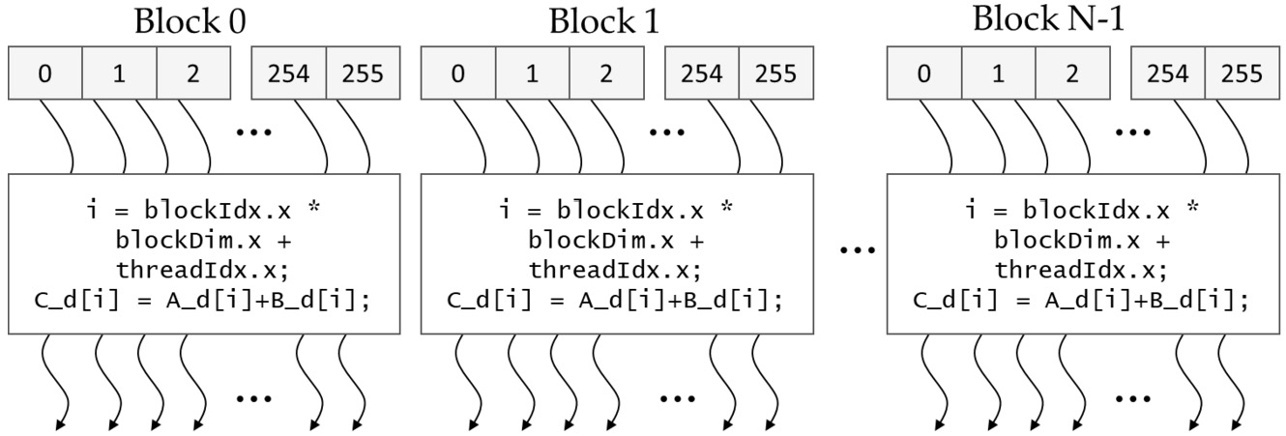
\includegraphics[width=\textwidth]{figs/ch2/2-9.png}
  \caption{网格中的所有线程执行相同的内核代码}
  \label{fig:2-9}
\end{figure}

\begin{quote}
\textbf{内置变量}

许多编程语言都有内置变量。这些变量具有特殊的含义和用途，通常由运行时系统
预先初始化，并且在程序中一般是只读的。程序员不应为了其他目的重新定义这些变量。
\end{quote}

在图 \ref{fig:2-9} 中，由于数据是一维向量，每个线程块都组织为一维线程数组。

每个块中的线程总数由内置变量 \code{blockDim.x} 给出。在图中，该值为 256。
\textbf{通常建议线程块中的线程总数是 32 的倍数}，这是出于硬件效率的考虑；本书后文会
再次讨论这一点。

CUDA 内核还可以访问另外两个内置变量 \code{threadIdx} 和 \code{blockIdx}，让
线程彼此区分，并确定每个线程需要处理的数据区域。\code{threadIdx} 为每个线程
提供块内的唯一坐标。在一维线程组织中只使用 \code{threadIdx.x}；图
\ref{fig:2-9} 中每个线程的小阴影方框显示了它的 \code{threadIdx.x} 值。每个块
中的第一个线程的值为 0，第二个线程的值为 1，第三个线程的值为 2，以此类推。

\code{blockIdx} 为一个块中的所有线程提供共同的块坐标。在图 \ref{fig:2-9} 中，
第一个块的所有线程的 \code{blockIdx.x} 值为 0，第二个块的值为 1，以此类推。
可以用电话系统作类比：\code{threadIdx.x} 类似本地电话号码，\code{blockIdx.x}
类似区号。两者结合起来，就能为全国范围内的每条电话线形成唯一的电话号码。同样，
每个线程也可以组合自己的 \code{threadIdx} 和 \code{blockIdx} 值，在整个网格
中生成唯一的全局索引。

\begin{quote}
\textbf{层次化组织}

像 CUDA 线程一样，现实世界中的许多系统也按层次组织。美国电话系统就是一个好
例子。最高层由许多“区域”组成，每个区域对应一个地理范围；同一区域内的所有
电话线共享一个三位数区号。一个电话区域有时会大于一座城市。例如，美国伊利诺伊
州中部的许多县和城市都属于同一电话区域，共享区号 217。

在一个区域内，每条电话线都有一个七位数的本地号码，因此每个区域最多约有一千万
个号码。可以把每条电话线看作一个 CUDA 线程，把区号看作 \code{blockIdx}，把
七位本地号码看作 \code{threadIdx}。这种层次化组织在保持局部性的同时，支持非常
大的电话线路数量；\textcolor{red}{拨打同一区域的号码时只需拨本地号码，偶尔拨打其他区域的号码
时才需要拨 1、区号和本地号码}。CUDA 线程的层次化组织也提供了一种局部性形式，
本书很快就会研究这种局部性。
\end{quote}

在图 \ref{fig:2-9} 中，使用下面的 C++ 语句计算唯一的全局索引 $i$：
\[
  i = \code{blockIdx.x} \times \code{blockDim.x} + \code{threadIdx.x}.
\]
本例中 \code{blockDim.x} 为 256。块 0 中线程的 $i$ 值范围为 0 到 255；块 1
中的范围为 256 到 511；块 2 中的范围为 512 到 767。也就是说，这三个块中线程
的 $i$ 值连续覆盖 0 到 767。由于每个线程使用 $i$ 访问 $A$、$B$ 和 $C$，这些
线程覆盖原始循环的前 768 次迭代。启动包含更多块的网格，就可以处理更长的向量；
启动包含 $n$ 个或更多线程的网格，就可以处理长度为 $n$ 的向量。

图 \ref{fig:2-10} 展示了向量加法的内核函数。注意，内核代码不采用 \code{_h} 和
\code{_d} 后缀约定，因为这里不存在混淆的可能；本章示例的内核代码不会访问任何
主机内存。\footnote{一般来说，内核代码可以通过称为统一虚拟地址（Unified
Virtual Address，UVA）的机制访问主机内存。该机制允许 GPU 访问主机内存，但带宽
低于访问自身设备全局内存；附录 C 会讨论这一机制。}

\begin{figure}[htbp]
  \centering
  \begin{lstlisting}[language=C++]
// Compute vector sum C = A + B
// Each thread performs one pair-wise addition
__global__
void vecAddKernel(float* A, float* B, float* C, int n) {
    int i = threadIdx.x + blockDim.x * blockIdx.x;
    if (i < n) {
        C[i] = A[i] + B[i];
    }
}
  \end{lstlisting}
  \caption{一个简单的向量加法内核函数}
  \label{fig:2-10}
\end{figure}

内核的语法遵循 C++ 标准，但有一些值得注意的扩展。首先，在
\code{vecAddKernel} 声明前有 CUDA 专用关键字 \code{__global__}。该关键字表示
这是一个内核，可以被调用来在设备上生成线程网格。

一般而言，CUDA C++ 用三个限定符关键字扩展 C++ 语言，可以在函数声明中使用。
图 \ref{fig:2-11} 总结了这些关键字的含义。\code{__global__} 表示所声明的
函数是 CUDA C++ 内核函数。注意，单词 \code{global} 两侧各有两个下划线。这种
内核函数在设备上执行，可以从主机调用；在支持动态并行性的 CUDA 系统中（从
Kepler 架构开始），也可以从设备调用。重要特征是，调用这种内核函数会在设备，
即 GPU 上启动一个新的线程网格。

\begin{figure}[htbp]
  \centering
  \begin{tabular}{>{\ttfamily}p{0.20\textwidth} p{0.18\textwidth} p{0.18\textwidth} p{0.28\textwidth}}
    \toprule
    限定符关键字 & 可从哪里调用 & 在哪里执行 & 由谁执行 \\
    \midrule
    \code{__host__}（默认） & 主机 & 主机 & 调用者主机线程 \\
    \code{__global__} & 主机（或设备） & 设备 & 新的设备线程网格 \\
    \code{__device__} & 设备 & 设备 & 调用者设备线程 \\
    \bottomrule
  \end{tabular}
  \caption{CUDA C++ 函数声明关键字}
  \label{fig:2-11}
\end{figure}

\code{__device__} 关键字表示所声明的是 CUDA 设备函数。设备函数在 GPU 设备上
执行，只能从内核函数或另一个设备函数中调用；它由调用它的设备线程执行，不会
启动新的设备线程。

\code{__host__} 关键字表示所声明的是 CUDA 主机函数。主机函数就是在主机上执行
的传统 C++ 函数，只能从另一个主机函数调用。如果声明中没有 CUDA 关键字，CUDA
程序中的所有函数默认都是主机函数。这很合理，因为许多 CUDA 应用是从只运行在
CPU 上的环境移植而来的；移植时，程序员会加入内核函数和设备函数，而原有函数
保持为主机函数。让函数默认成为主机函数，可以免去程序员修改所有原有函数声明
的繁琐工作。

既然所有函数默认都是主机函数，为什么还需要 \code{__host__} 关键字？有时，程序
员希望一个函数同时能够在主机和设备上使用。标记 \code{__device__} 会使函数只
在设备上可用；要让它在两者上都可用，可以在函数声明中同时使用 \code{__host__}
和 \code{__device__}。这种组合会告诉编译系统，为同一个函数生成两份目标代码：
一份在主机上执行，只能从主机函数调用；另一份在设备上执行，只能从设备函数或
内核函数调用。当同一份函数源代码需要重新编译以生成设备版本时，这种能力非常
有用，许多用户库函数可能属于这一类。

图 \ref{fig:2-10} 中 \code{vecAdd} 内核使用的第二个值得注意的 CUDA C++ 扩展，
是内置变量 \code{threadIdx}、\code{blockIdx} 和 \code{blockDim}。回顾一下，
所有线程执行相同的内核代码，因此必须有办法让线程彼此区分，并把每个线程导向
数据的特定部分。这些内置变量让线程能够访问硬件寄存器，从而获得标识自身的坐标。
不同线程会看到其 \code{threadIdx.x}、\code{blockIdx.x} 和 \code{blockDim.x}
变量的不同值。

利用内置变量计算出的全局索引（图 \ref{fig:2-10} 第 5 行）被写入一个类型为
\code{int} 的自动（局部）变量 $i$。\footnote{不同的 C 和 C++ 程序员在声明用于
表示数组索引、数组大小、循环迭代计数器和循环边界的变量时，可能选择 \code{int}
或 \code{unsigned int}。使用 \code{unsigned int} 能明确表明这些变量绝不应为
负数，并可能触发有助于防止错误的编译器警告。另一方面，在执行减法，或在算术
运算中混用 \code{unsigned int} 与其他 \code{int} 变量时，使用 \code{int} 可以
避免错误。此外，由于 \code{int} 溢出的行为未定义，编译器可以在优化时利用这一
事实。本书在上述声明中有时使用 \code{int}，有时使用 \code{unsigned int}；读者
在自己的实现中可采用任一种风格。} \textbf{在 CUDA 内核函数中，自动变量对每个线程都是
私有的。}
也就是说，每个线程都会生成一份 $i$；如果网格启动了 10,000 个线程，就会有
10,000 份 $i$，每个线程一份。一个线程赋给自己 $i$ 的值，其他线程不可见。本书
第 5 章会更详细地讨论这些自动变量。

比较图 \ref{fig:2-4} 和图 \ref{fig:2-10}，可以发现 CUDA 内核有一个重要特点：
图 \ref{fig:2-10} 中没有对应原始循环的 \code{for} 循环。读者可能会问，循环
去哪儿了？答案是，循环现在被线程网格替代。整个网格构成循环的等价物，网格中的
每个线程对应原始循环的一次迭代。这有时称为循环并行性，即把原来顺序代码的迭代
交给线程并行执行。

注意，\code{vecAddKernel} 中有 \code{if (i < n)}。这是因为并非所有向量长度都
能表示为块大小的整数倍。例如，向量长度为 100，最小的高效线程块维度为 32，
选择块大小 32 时，需要启动 4 个线程块才能处理全部 100 个向量元素。然而，4 个
块共包含 128 个线程；必须禁止最后 28 个线程执行原程序没有要求的工作。由于所有
线程执行相同代码，它们都会把自己的 $i$ 值与 $n=100$ 比较。借助
\code{if (i < n)}，前 100 个线程执行加法，最后 28 个线程不执行，从而允许内核
处理任意长度的向量。

\section{调用内核函数}
\label{sec:calling-kernel-functions}

实现内核函数后，下一步是在主机代码中调用它，以启动线程网格。图
\ref{fig:2-12} 展示了调用向量加法内核的主机代码。当主机代码调用内核时，会
通过执行配置参数设置网格和线程块的维度。配置参数放在传统 C++ 函数参数之前的
\code{<<<} 和 \code{>>>} 括号之间。第一个配置参数给出网格中的块数，第二个
参数指定每个块中的线程数；本例中每个块有 256 个线程。

\begin{figure}[htbp]
  \centering
  \begin{lstlisting}[language=C++]
void vecAdd(float* A, float* B, float* C, int n) {
    // Allocation and copying of A_d, B_d, and C_d omitted
    ...
    // Launch ceil(n/256) blocks with 256 threads per block
    vecAddKernel<<<ceil(n/256.0), 256>>>(A_d, B_d, C_d, n);
}
  \end{lstlisting}
  \caption{包含向量加法内核调用语句的主机代码示例}
  \label{fig:2-12}
\end{figure}


为了保证网格中的线程足以覆盖所有向量元素，需要把网格块数设置为所需线程数
（这里是 $n$）除以线程块大小（这里是 256）后的向上取整，即天花板除法。实现
天花板除法有很多方法；一种方法是对 \code{n/256.0} 应用 C++ 的 \code{ceil}
函数。使用浮点数 256.0 可以确保除法结果为浮点值，使 \code{ceil} 能正确向上
取整。例如，要生成 1000 个线程，就启动
\[
  \code{ceil(1000/256.0)}=4
\]
个线程块，结果是 $4\times256=1024$ 个线程。结合内核中的
\code{if (i < n)}，前 1000 个线程会对 1000 个向量元素执行加法，其余 24 个
线程不执行。

图 \ref{fig:2-13} 展示了 \code{vecAdd} 函数中的最终主机代码；它补全了图
\ref{fig:2-5} 中的骨架代码。图 \ref{fig:2-10} 和图 \ref{fig:2-13} 共同展示
了一个同时包含主机代码和设备内核的简单 CUDA 程序。

\begin{figure}[htbp]
  \centering
  \begin{lstlisting}[language=C++]
void vecAdd(float* A, float* B, float* C, int n) {
    float *A_d, *B_d, *C_d;
    int size = n * sizeof(float);

    cudaMalloc((void**)&A_d, size);
    cudaMalloc((void**)&B_d, size);
    cudaMalloc((void**)&C_d, size);

    cudaMemcpy(A_d, A, size, cudaMemcpyHostToDevice);
    cudaMemcpy(B_d, B, size, cudaMemcpyHostToDevice);

    vecAddKernel<<<ceil(n/256.0), 256>>>(A_d, B_d, C_d, n);

    cudaMemcpy(C, C_d, size, cudaMemcpyDeviceToHost);

    cudaFree(A_d);
    cudaFree(B_d);
    cudaFree(C_d);
}
  \end{lstlisting}
  \caption{向量加法内核调用语句}
  \label{fig:2-13}
\end{figure}

这份源代码把线程块大小硬编码为每块 256 个线程，但使用的线程块数量取决于向量
长度 $n$。如果 $n=750$，就使用 3 个线程块；如果 $n=4000$，就使用 16 个线程
块；如果 $n=2{,}000{,}000$，就使用 7813 个线程块。注意，所有线程块都操作
向量的不同部分，可以按任意顺序执行。\textbf{程序员不能对执行顺序作任何假设}。

执行资源较少的小型 GPU 可能一次只并行执行其中一两个线程块；较大的 GPU 可能
同时执行 128 或 256 个线程块。这使 CUDA 内核的执行速度能够随硬件扩展：同一份
代码在小型 GPU 上以较低速度运行，在大型 GPU 上以较高速度运行。第 4 章会再次
讨论这一点。

\section{编译}
\label{sec:compilation}

我们已经看到，实现 CUDA C++ 内核需要使用并非 C++ 标准组成部分的各种扩展。一旦
代码中使用了这些扩展，就不能再交给传统 C++ 编译器；必须使用能够识别和理解这些
扩展的编译器，例如 NVCC（NVIDIA CUDA Compiler）。

如图 \ref{fig:2-14} 顶部所示，NVCC 处理 CUDA C++ 程序，并利用 CUDA 关键字把
主机代码和设备代码分离。主机代码是普通 C++ 代码，由标准 C/C++ 编译器编译，
并作为传统 CPU 进程运行。标记了 CUDA 关键字、用于声明 CUDA 内核及其相关设备
函数和数据结构的设备代码，则由 NVCC 编译为称为 PTX 的虚拟二进制文件。随后，
NVCC 的运行时组件会进一步把这些 PTX 文件编译为真正的目标文件，并在支持 CUDA
的 GPU 设备上执行。

\begin{figure}[htbp]
  \centering
  \begin{tabular}{c}
    \textbf{包含 CUDA 扩展的 C++ 程序}\\
    $\downarrow$\\
    \fbox{\parbox{0.55\textwidth}{\centering NVCC 编译器}}\\[0.4em]
    \begin{tabular}{c@{\qquad}c}
      $\swarrow$ 主机代码 & 设备代码（PTX） $\searrow$\\
      \fbox{\parbox{0.31\textwidth}{\centering 主机 C++ 预处理器、编译器/链接器}}
      &
      \fbox{\parbox{0.31\textwidth}{\centering 设备即时编译器}}\\
      $\searrow$ & $\swarrow$
    \end{tabular}\\[0.4em]
    \fbox{\parbox{0.65\textwidth}{\centering 包含 CPU 和 GPU 的异构计算平台}}
  \end{tabular}
  \caption{CUDA C++ 程序的编译过程概览}
  \label{fig:2-14}
\end{figure}

\section{小结}
\label{sec:chapter-2-summary}

本章快速、简化地概览了 CUDA C++ 编程模型。CUDA C++ 扩展 C++ 语言以支持并行
计算，本章讨论了这些扩展中的一个基本子集。为方便读者，现将这些扩展总结如下。

\paragraph{函数声明。}
CUDA C++ 扩展 C++ 函数声明语法，以支持异构并行计算。图 \ref{fig:2-11} 总结了
这些扩展。使用 \code{__global__}、\code{__device__} 或 \code{__host__} 中的
一个，程序员可以指示编译器生成内核函数、设备函数或主机函数。没有这些关键字的
函数声明默认是主机函数。如果函数声明同时使用 \code{__host__} 和
\code{__device__}，编译器会生成两个版本，一个用于设备，一个用于主机。

\paragraph{内核调用与网格启动。}
CUDA C++ 用被 \code{<<<} 和 \code{>>>} 括号包围的内核执行配置参数扩展 C++
函数调用语法。这些执行配置参数只在调用内核函数、启动线程网格时使用。本章讨论
了定义网格维度和每个块维度的执行配置参数；关于内核启动扩展以及其他类型执行
配置参数的更多细节，请参阅 CUDA 编程指南 \cite{cuda2025-ch2}。

\paragraph{内置（预定义）变量。}
CUDA 内核可以访问一组内置只读变量，让每个线程区分自己与其他线程，并确定自己
需要处理的数据区域。本章讨论了 \code{threadIdx}、\code{blockDim} 和
\code{blockIdx}；第 3 章将进一步讨论如何使用这些变量，在处理多维数据时管理
多维块和网格。

\paragraph{运行时 API。}
CUDA 支持一组应用程序接口（Application Programming Interface，API）函数，为
CUDA C++ 程序提供服务。本章讨论的服务包括 \code{cudaMalloc}、\code{cudaFree}
和 \code{cudaMemcpy}；这些函数由主机代码调用，分别代表调用程序分配设备全局
内存、释放设备全局内存，以及在主机和设备之间传送数据。关于其他 CUDA API 函数，
请参阅 CUDA C++ 编程指南 \cite{cuda2025-ch2}。

本章的目标是介绍 CUDA C++ 的核心概念，以及编写简单 CUDA 程序所需的基本 CUDA
到 C++ 的扩展。本章绝不是 CUDA 全部特性的完整说明；本书后续部分还会介绍更多
特性。不过，我们强调的是这些特性所支持的关键并行计算概念。对于并行编程技术
的代码示例，我们只会介绍足够使用的 CUDA C++ 特性。一般而言，我们始终建议
读者查阅 CUDA C++ 编程指南 \cite{cuda2025-ch2}，了解最新特性的更多细节。

\section{练习}
\label{sec:chapter-2-exercises}

\begin{enumerate}[label=\arabic*.,leftmargin=2.7em]
  \item 如果希望网格中的每个线程计算向量加法的一个输出元素，那么在内核函数中，
  把线程/块索引映射到数据索引 $i$ 的表达式是什么？
  \begin{enumerate}[label=\alph*.,leftmargin=2.2em]
    \item \code{i = threadIdx.x + threadIdx.y;}
    \item \code{i = blockIdx.x + threadIdx.x;}
    \item \code{i = blockIdx.x * blockDim.x + threadIdx.x;}
    \item \code{i = blockIdx.x * threadIdx.x;}
  \end{enumerate}

  \item 假设希望每个线程计算向量加法中相邻的两个元素。把线程/块索引映射到线程
  要处理的第一个元素的数据索引 $i$ 的表达式是什么？
  \begin{enumerate}[label=\alph*.,leftmargin=2.2em]
    \item \code{i = blockIdx.x * blockDim.x + threadIdx.x + 2;}
    \item \code{i = blockIdx.x * threadIdx.x * 2;}
    \item \code{i = (blockIdx.x * blockDim.x + threadIdx.x) * 2;}
    \item \code{i = blockIdx.x * blockDim.x * 2 + threadIdx.x;}
  \end{enumerate}

  \item 希望每个线程计算两个元素。每个线程块处理由两个区段组成的、连续的
  $2\times\code{blockDim.x}$ 个元素。块中的所有线程先处理第一个区段，每个线程
  处理一个元素；然后它们一起移动到下一个区段，每个线程再处理一个元素。假设
  变量 $i$ 是线程要处理的第一个元素的索引，那么把线程/块索引映射到第一个
  元素数据索引的表达式是什么？
  \begin{enumerate}[label=\alph*.,leftmargin=2.2em]
    \item \code{i = blockIdx.x * blockDim.x + threadIdx.x + 2;}
    \item \code{i = blockIdx.x * threadIdx.x * 2;}
    \item \code{i = (blockIdx.x * blockDim.x + threadIdx.x) * 2;}
    \item \code{i = blockIdx.x * blockDim.x * 2 + threadIdx.x;}
  \end{enumerate}

  \item 对于一次向量加法，向量长度为 8000，每个线程计算一个输出元素，线程块
  大小为 1024。程序员把内核调用配置为覆盖所有输出元素所需的最少线程块数。
  网格中有多少个线程？
  \begin{enumerate}[label=\alph*.,leftmargin=2.2em]
    \item 8000
    \item 8196
    \item 8192
    \item 8200
  \end{enumerate}

  \item 要为包含 $v$ 个整数元素的数组分配设备全局内存。
  \code{cudaMalloc} 的第二个参数应使用哪个表达式？
  \begin{enumerate}[label=\alph*.,leftmargin=2.2em]
    \item \code{n}
    \item \code{v}
    \item \code{n * sizeof(int)}
    \item \code{v * sizeof(int)}
  \end{enumerate}

  \item 如果希望分配一个包含 $n$ 个浮点元素的数组，并让浮点指针变量
  \code{A_d} 指向所分配的内存，\code{cudaMalloc} 调用的第一个参数应使用什么
  表达式？
  \begin{enumerate}[label=\alph*.,leftmargin=2.2em]
    \item \code{n}
    \item \code{(void *) A_d}
    \item \code{*A_d}
    \item \code{(void **) &A_d}
  \end{enumerate}

  \item 如果希望把 3000 字节数据从主机数组 \code{A_h}（\code{A_h} 指向源数组
  的第 0 个元素）复制到设备数组 \code{A_d}（\code{A_d} 指向目标数组的第 0 个
  元素），CUDA 中适合进行该复制的 API 调用是什么？
  \begin{enumerate}[label=\alph*.,leftmargin=2.2em]
    \item \code{cudaMemcpy(3000, A_h, A_d, cudaMemcpyHostToDevice);}
    \item \code{cudaMemcpy(A_h, A_d, 3000, cudaMemcpyDeviceToHost);}
    \item \code{cudaMemcpy(A_d, A_h, 3000, cudaMemcpyHostToDevice);}
    \item \code{cudaMemcpy(3000, A_d, A_h, cudaMemcpyHostToDevice);}
  \end{enumerate}

  \item 应如何声明变量 \code{err}，才能适当地接收 CUDA API 调用返回的值？
  \begin{enumerate}[label=\alph*.,leftmargin=2.2em]
    \item \code{int err;}
    \item \code{cudaError err;}
    \item \code{cudaError_t err;}
    \item \code{cudaSuccess_t err;}
  \end{enumerate}

  \item 考虑图 \ref{fig:2-15} 中的 CUDA 内核及调用它的主机函数。

  \begin{figure}[htbp]
    \centering
    \begin{lstlisting}[language=C++]
__global__ void foo_kernel(float* a, float* b, unsigned int N) {
    unsigned int i = blockIdx.x * blockDim.x + threadIdx.x;
    if (i < N) {
        b[i] = 2.7f * a[i] - 4.3f;
    }
}
void foo(float* a_d, float* b_d) {
    unsigned int N = 200000;
    foo_kernel<<<(N + 128 - 1)/128, 128>>>(a_d, b_d, N);
}
    \end{lstlisting}
    \caption{练习题 9 的 CUDA 代码}
    \label{fig:2-15}
  \end{figure}

  \begin{enumerate}[label=\alph*.,leftmargin=2.2em]
    \item 每个块中的线程数是多少？
    \item 网格中的线程总数是多少？
    \item 网格中的块数是多少？
    \item 执行第 02 行代码的线程数是多少？
    \item 执行第 04 行代码的线程数是多少？
  \end{enumerate}

  \item 一位新的 CUDA 程序员对 CUDA 感到沮丧。他抱怨 CUDA 太繁琐：自己计划
  在主机和设备上都执行的许多函数，必须分别声明两次，一次声明为主机函数，一次
  声明为设备函数。你会如何帮助这位新程序员？
\end{enumerate}

\begin{chapterbibliography}{3}

\bibitem{patt2020}
Y. N. Patt and S. J. Patel.
\emph{Introduction to Computing Systems: From Bits and Gates to C and Beyond}.
McGraw Hill Publisher, 2020, 2000, 2004.

\bibitem{atallah1998}
M. J. E. Atallah.
\emph{Algorithms and Theory of Computation Handbook}.
CRC Press, 1998.

\bibitem{cuda2025-ch2}
NVIDIA.
\emph{CUDA C++ Programming Guide}, Release 13.0, 2025.
\url{https://docs.nvidia.com/cuda/cuda-c-programming-guide}.

\end{chapterbibliography}

\chapter{多维网格与数据}
\label{chap:multidimensional-grids-and-data}

\setcounter{footnote}{0}

第二章中，我们学习了如何编写一个简单的 CUDA C++ 程序：调用内核函数，启动一个
处理一维数组元素的一维线程网格。内核规定网格中每个线程要执行的语句。本章将更
一般地考察线程的组织方式，并学习如何使用线程和线程块处理多维数组。全章贯穿
多个例子，包括把彩色图像转换为灰度图像、模糊图像以及矩阵乘法。这些例子也将
帮助读者熟悉数据并行推理，为后续讨论 GPU 架构、内存组织和性能优化做好准备。

\section{多维网格组织}
\label{sec:multidimensional-grid-organization}

在 CUDA 中，网格中的所有线程都执行同一个内核函数，并依靠自己的坐标（即线程
索引）彼此区分，同时确定要处理的数据区域。正如第二章所见，这些线程按两级层次
组织：一个网格由一个或多个线程块组成，每个线程块又由一个或多个线程组成。同一
线程块中的所有线程共享相同的块索引，该索引可以通过内置变量 \code{blockIdx}
访问。每个线程还有自己的线程索引，可以通过内置变量 \code{threadIdx} 访问。
线程执行内核函数时，引用 \code{blockIdx} 和 \code{threadIdx} 会得到该线程的
坐标。内核调用语句中的执行配置参数指定网格和每个线程块的维度；这些维度可以
通过内置变量 \code{gridDim} 和 \code{blockDim} 访问。

一般而言，网格是一个三维线程块数组，而每个线程块又是一个三维线程数组。调用
内核时，程序需要指定网格大小以及每个线程块在各个维度上的大小。这些大小通过
内核调用语句中的执行配置参数（位于 \code{<<< ... >>>} 之间）指定。第一个
执行配置参数以线程块数量为单位指定网格的维度，第二个以线程数量为单位指定
每个线程块的维度。每个参数的类型都是 \code{dim3}，这是一种包含三个整数
元素 \code{x}、\code{y} 和 \code{z} 的向量类型；三个元素分别指定三个维度的
大小。如果程序使用的维度少于三个，只需把未使用维度的大小设为 1。

例如，下面的主机代码调用 \code{vecAddKernel}，生成一个一维网格；该网格包含
32 个线程块，每个线程块包含 128 个线程：

\begin{lstlisting}[language=C++]
dim3 dimGrid(32, 1, 1);
dim3 dimBlock(128, 1, 1);
vecAddKernel<<<dimGrid, dimBlock>>>(...);
\end{lstlisting}

在这个例子中，网格中的线程总数为
\[
  128 \times 32 = 4096.
\]
注意，\code{dimBlock} 和 \code{dimGrid} 是由程序员在主机代码中定义的变量。
只要类型为 \code{dim3}，它们可以使用任何合法的 C++ 变量名。例如，下面的
语句与前面的语句实现相同的效果：

\begin{lstlisting}[language=C++]
dim3 dog(32, 1, 1);
dim3 cat(128, 1, 1);
vecAddKernel<<<dog, cat>>>(...);
\end{lstlisting}

网格和线程块的维度也可以根据其他变量计算。例如，图 2.12 中的内核调用可以
改写为：

\begin{lstlisting}[language=C++]
dim3 dimGrid(ceil(n/256.0), 1, 1);
dim3 dimBlock(256, 1, 1);
vecAddKernel<<<dimGrid, dimBlock>>>(...);
\end{lstlisting}

这样，线程块数量就可以随向量长度变化，使网格拥有足够的线程覆盖所有向量元素。
在本例中，程序员选择把线程块大小固定为 256；调用内核时变量 \code{n} 的值
决定网格的维度。如果 \code{n} 等于 1000，网格包含 4 个线程块；如果 \code{n}
等于 4000，网格包含 16 个线程块。在这两种情况下，线程数都足以覆盖所有向量
元素。网格启动后，网格和线程块的维度在整个网格执行完毕之前保持不变。

为了方便一维网格和一维线程块的调用，CUDA 提供了一种特殊的简写形式。不使用
\code{dim3} 变量时，可以直接使用算术表达式指定一维网格和线程块的配置。在
这种情况下，CUDA 编译器把算术表达式作为 \code{x} 维度，并假定 \code{y} 和
\code{z} 维度均为 1。因此，图 2.12 中的内核调用可以写成：

\begin{lstlisting}[language=C++]
vecAddKernel<<<ceil(n/256.0), 256>>>(...);
\end{lstlisting}

熟悉 C++ 的读者会发现，这种一维配置的“简写”利用了 C++ 构造函数和默认参数
的工作方式。\code{dim3} 构造函数的参数默认值为 1。当只传入一个值而期望
\code{dim3} 时，该值传给构造函数的第一个参数，第二、第三个参数使用默认值 1。
因此得到一个一维网格或线程块，其 \code{x} 维度大小就是传入的值，\code{y} 和
\code{z} 维度大小为 1。

在内核函数中，变量 \code{gridDim} 和 \code{blockDim} 的 \code{x} 字段会根据
执行配置参数预先初始化。例如，如果 \code{n} 等于 4000，那么在
\code{vecAddKernel} 内引用 \code{gridDim.x} 和 \code{blockDim.x}，得到的值
分别为 16 和 256。注意，与主机代码中的 \code{dim3} 变量不同，内核函数中的
这些变量名属于 CUDA C++ 规范，不能更改。也就是说，\code{gridDim} 和
\code{blockDim} 是内置变量，始终反映网格和线程块的维度。

在 CUDA C++ 中，\code{gridDim.x} 的允许取值范围为 1 到 $2^{31}-1$；
\code{gridDim.y} 和 \code{gridDim.z} 的允许取值范围为 1 到
$2^{16}-1=65{,}535$。同一线程块中的所有线程共享 \code{blockIdx.x}、
\code{blockIdx.y} 和 \code{blockIdx.z} 的值。在所有线程块之间，
\code{blockIdx.x} 的取值范围为 0 到 \code{gridDim.x-1}，
\code{blockIdx.y} 的取值范围为 0 到 \code{gridDim.y-1}，
\code{blockIdx.z} 的取值范围为 0 到 \code{gridDim.z-1}。

下面转而讨论线程块的配置。每个线程块组织成一个三维线程数组。

把 \code{blockDim.z} 设为 1，就可以创建二维线程块。
像向量加法示例那样，一维线程块满足
\[
  \code{blockDim.y}=1,\qquad \code{blockDim.z}=1.
\]

前文已经提到，同一网格中的所有线程块具有相同的维度和大小。线程块每个维度
的线程数量由内核调用的第二个执行配置参数指定。在内核中，可以通过
\code{blockDim} 的 \code{x}、\code{y} 和 \code{z} 字段访问这一配置。

在当前 CUDA 系统中，一个线程块的总大小限制为 1024 个线程。只要线程总数不超过
1024，这些线程可以以任意方式分布在三个维度中。例如，下面的
\code{blockDim} 值都是允许的：
\[
  (512,1,1),\qquad (8,16,4),\qquad (32,16,2).
\]
另一方面，\code{blockDim} 为 $(32,32,2)$ 时线程总数超过 1024，因此不允许。

网格及其线程块不需要具有相同的维度。网格可以比线程块维度更高，反之亦然。
例如，图 \ref{fig:3-1} 展示了一个小型示例，其中
\code{gridDim} 为 $(2,2,1)$，\code{blockDim} 为 $(4,2,2)$。可以使用下面的
主机代码创建该网格：

\begin{lstlisting}[language=C++]
dim3 dimGrid(2, 2, 1);
dim3 dimBlock(4, 2, 2);
KernelFunction<<<dimGrid, dimBlock>>>(...);
\end{lstlisting}

\begin{figure}[htbp]
  \centering
  \begingroup
  \scriptsize
  \setlength{\tabcolsep}{4pt}
  \begin{tabular}{c@{\hspace{0.8em}}c}
    \fbox{\begin{minipage}{0.23\textwidth}
      \centering
      \textbf{主机}\\[0.3em]
      \fbox{\code{Kernel 1}}\\[0.8em]
      \fbox{\code{Kernel 2}}
    \end{minipage}}
    &
    \fbox{\begin{minipage}{0.58\textwidth}
      \centering
      \textbf{设备}\\[0.2em]
      \fbox{\begin{minipage}{0.45\textwidth}
        \centering
        \textbf{网格 1（Grid 1）}\\[0.2em]
        \begin{tabular}{cc}
          \fbox{块 $(0,0)$} & \fbox{块 $(0,1)$}\\
          \fbox{块 $(1,0)$} & \fbox{块 $(1,1)$}
        \end{tabular}
      \end{minipage}}\\[0.6em]
      \fbox{\begin{minipage}{0.45\textwidth}
        \centering
        \textbf{网格 2（Grid 2）}\\[0.2em]
        \fbox{\begin{minipage}{0.9\textwidth}
          \centering
          \textbf{块 $(1,1)$ 展开}\\
          $4\times2\times2=16$ 个线程\\
          \code{threadIdx=(z,y,x)}
        \end{minipage}}
      \end{minipage}}
    \end{minipage}}
  \end{tabular}
  \endgroup
  \caption{CUDA 多维网格组织示例（依据原书图 3.1 重绘的概念示意）}
  \label{fig:3-1}
\end{figure}

图 \ref{fig:3-1} 中的网格由 4 个线程块组成，排列成一个 $2\times2$ 数组。
每个线程块使用 $(\code{blockIdx.y},\code{blockIdx.x})$ 标记。例如，块
$(1,0)$ 的 \code{blockIdx.y}=1，\code{blockIdx.x}=0。需要注意，块和线程标签
的排列顺序是最高维度在前。这与设置执行配置参数时代码使用的顺序相反；代码中
最低维度在前。用这种相反的顺序标记块，更适合说明线程坐标如何映射到多维数据
的索引。

每个 \code{threadIdx} 也包含三个字段：x 坐标 \code{threadIdx.x}、y 坐标
\code{threadIdx.y} 和 z 坐标 \code{threadIdx.z}。图 \ref{fig:3-1} 展示了
线程块内部的组织方式。在这个例子中，每个线程块组织成一个 $4\times2\times2$
的线程数组。由于网格中的所有线程块具有相同的维度，图中只展开其中一个线程块。
图 \ref{fig:3-1} 展开块 $(1,1)$，展示其中的 16 个线程。例如，线程 $(1,0,2)$
具有 \code{threadIdx.z}=1、\code{threadIdx.y}=0 和 \code{threadIdx.x}=2。
在这个例子中，网格共有 4 个线程块，每个线程块 16 个线程，总计 64 个线程。

\noindent\textbf{译者注：}原书相应说明中有一处疑似排印错误，写作
\code{threadId.x}；CUDA C++ 的内置变量实际是 \code{threadIdx.x}，本译稿按
正确标识符规范化。
这里使用很小的数字只是为了让图示保持简单；典型 CUDA 网格包含数千到数百万个
线程。

\section{将线程映射到多维数据}
\label{sec:mapping-threads-to-multidimensional-data}

选择一维、二维还是三维线程组织，通常取决于数据的性质。例如，图片是由像素组成
的二维数组，使用由二维线程块组成的二维网格，通常很适合处理图片中的像素。图
\ref{fig:3-2} 展示了这种处理方式，输入图片 \code{Pin} 的大小为 $62\times76$
（垂直方向或 y 方向有 62 个像素，水平方向或 x 方向有 76 个像素）。假设我们
选择 $16\times16$ 的线程块，即 x 方向和 y 方向各有 16 个线程。需要在 y 方向
使用 4 个线程块，在 x 方向使用 5 个线程块，因此总共需要 $4\times5=20$ 个
线程块，如图 \ref{fig:3-2} 所示。粗线表示线程块边界；本概念重绘用文字标出
实际像素区和线程覆盖区，具体的有效线程分类见图 \ref{fig:3-5}。每个线程负责处理
一个像素，其 y、x 坐标由 \code{blockIdx}、
\code{blockDim} 和 \code{threadIdx} 的值推导得到。

\footnote{本书始终按多维数据的降序维度书写其尺寸：先写 z 维，再写 y 维，最后
写 x 维。例如，对于垂直方向（或 y 方向）有 $n$ 个像素、水平方向（或 x 方向）
有 $m$ 个像素的图片，我们将其写作 $n\times m$。这遵循 C++ 多维数组的索引
约定。例如，正文和图中可以简写 $P[y][x]$ 为 $P_{y,x}$。遗憾的是，这与
\code{gridDim} 和 \code{blockDim} 中数据维度的排列顺序相反。当根据要处理的
多维数组定义线程网格的维度时，这种差异尤其容易造成混淆。}

垂直（行）坐标为：
\[
  \code{blockIdx.y} \times \code{blockDim.y} + \code{threadIdx.y}.
\]
水平（列）坐标为：
\[
  \code{blockIdx.x} \times \code{blockDim.x} + \code{threadIdx.x}.
\]

\begin{figure}[htbp]
  \centering
  \fbox{\begin{minipage}{0.88\textwidth}
    \centering
    \textbf{输入图片：$62\times76$}\\[0.4em]
    \begin{tabular}{c|c|c|c|c}
      \multicolumn{5}{c}{x 方向：5 个线程块，每块 $16\times16$}\\
      \hline
      \rule{0pt}{1.1em}块 & 块 & 块 & 块 & 块\\ \hline
      块 & 块 & 块 & 块 & 块\\ \hline
      块 & 块 & 块 & 块 & 块\\ \hline
      块 & 块 & 块 & 块 & 块\\ \hline
    \end{tabular}\\[0.3em]
    y 方向：4 个线程块；实际像素区域为 $62\times76$，
    线程覆盖区域为 $64\times80$
  \end{minipage}}
  \caption{使用二维线程网格处理输入图片 \code{Pin}（$62\times76$，
  依据原书图 3.2 重绘的概念示意）}
  \label{fig:3-2}
\end{figure}

例如，块 $(1,0)$ 中线程 $(0,0)$ 要处理的 \code{Pin} 元素可由下面的索引得到：
\[
\begin{aligned}
\text{行索引}
  &=\code{blockIdx.y * blockDim.y}
    +\code{threadIdx.y}\\
  &=1\times16+0=16,\\
\text{列索引}
  &=\code{blockIdx.x * blockDim.x}
    +\code{threadIdx.x}\\
  &=0\times16+0=0.
\end{aligned}
\]
因此，该线程处理的元素是 $P_{\mathrm{in}}[16,0]$。

注意，图 \ref{fig:3-2} 中 y 方向多生成了 2 个线程，x 方向多生成了 4 个线程。
也就是说，为了处理 $62\times76$ 个像素，我们总共生成了 $64\times80$ 个线程。
这与一维内核 \code{vecAddKernel} 使用 4 个 256 线程块处理 1000 个元素时
的情况类似。回顾第二章图 2.10，需要用 \code{if} 语句防止多出的 24 个线程
产生影响。同样，图片处理内核也应检查线程的垂直索引和水平索引是否落在有效
像素范围内。

假设主机代码使用整数变量 \code{n} 记录 y 方向的像素数，使用另一个整数变量
\code{m} 记录 x 方向的像素数。进一步假设输入图片数据已经复制到设备全局内存，
可以通过指针变量 \code{Pin_d} 访问；输出图片已经分配在设备内存中，可以通过
\code{Pout_d} 访问。下面的主机代码调用二维内核 \code{colorToGrayscaleConversion}
处理图片：

\begin{lstlisting}[language=C++]
dim3 dimGrid(ceil(m/16.0), ceil(n/16.0), 1);
dim3 dimBlock(16, 16, 1);
colorToGrayscaleConversion<<<dimGrid, dimBlock>>>(
    Pout_d, Pin_d, m, n);
\end{lstlisting}

\noindent\textbf{译者注：}原书此处的主机调用顺序与图 3.4 中的内核形参声明
\code{Pout, Pin} 相反。为使示例按该声明正确工作，本译稿将调用顺序校正为
\code{Pout_d, Pin_d}；这一处改动特此注明。

为简单起见，本例把线程块维度固定为 $16\times16$。另一方面，网格维度取决于
图片的尺寸。处理一张 $1500\times2000$（300 万像素）的图片时，需要生成
11,750 个线程块：y 方向 94 个，x 方向 125 个。在内核函数中引用
\code{gridDim.x}、\code{gridDim.y}、\code{blockDim.x} 和 \code{blockDim.y}，
得到的值分别为 125、94、16 和 16。

在展示内核代码之前，需要先理解 C 和 C++ 语句如何访问动态分配的多维数组。理想
情况下，我们希望把 \code{Pin_d} 当作二维数组访问，使第 $j$ 行、第 $i$ 列的
元素可以写成 \code{Pin_d[j][i]}。但是，CUDA C++ 所基于的 C++ 标准要求，在
把 \code{Pin} 当作二维数组访问时，列数必须在编译期已知。对于动态分配的数组，
这个信息在编译期并不知道。事实上，使用动态数组的部分原因正是允许数组大小和
维度根据运行时的数据大小变化。因此，动态分配二维数组的列数在编译期未知，是
设计所决定的。结果是，在当前 CUDA C++ 中，程序员需要显式地把动态分配的二维
数组线性化（或“展平”）为等价的一维数组。

实际上，C 和 C++ 中的所有多维数组最终都会被线性化。这是因为现代计算机使用
“扁平”的内存空间（见“内存空间”侧栏）。对于静态分配的数组，编译器允许程序员
使用 \code{Pin_d[j][i]} 这样的高维索引语法访问元素；在底层，编译器会把它们
线性化为等价的一维数组，并把多维索引语法转换为一维偏移量。对于动态分配的数组，
由于编译期缺少执行这种转换所需的维度信息，这项转换就留给程序员完成。

\begin{quote}
\textbf{内存空间}

内存空间是对现代计算机中处理器如何访问内存的一种简化视图。通常，每个正在运行
的应用程序都有自己的内存空间。应用要处理的数据以及为应用执行的指令，都存放
在该内存空间的位置中。每个位置通常可以容纳一个字节，并具有一个地址。需要
多个字节的变量——例如占 4 字节的 \code{float} 和占 8 字节的 \code{double}——
存放在连续的字节位置中。访问内存空间中的数据值时，处理器给出起始地址（起始
字节位置的地址）以及所需的字节数。

大多数现代计算机至少有 $4$G 个按字节编址的位置。这里，每个 G 表示的位置数为
\[
  1{,}073{,}741{,}824=2^{30}.
\]
所有位置都带有从 0 到最大编号的地址。由于每个位置只有一个地址，我们称这种
内存空间具有“扁平”组织。因此，所有多维数组最终都会被“展平”为等价的一维数组。
C++ 程序员虽然可以使用多维数组语法访问元素，但编译器会把这种访问转换为一个
指向数组起始元素的基指针，以及根据多维索引计算得到的一维偏移量。
\end{quote}

二维数组至少有两种线性化方式。一种方式是把同一行的所有元素放在连续位置中，
再把各行依次放入内存空间。这种布局称为行主序（row-major layout），如图
\ref{fig:3-3} 所示。为提高可读性，我们用 $M_{j,i}$ 表示矩阵 $M$ 第 $j$ 行、
第 $i$ 列的元素。它等价于 C++ 中的 \code{M[j][i]}，但在正文和图中更易读。
图 \ref{fig:3-3} 展示了一个 $4\times4$ 矩阵 $M$ 被线性化为包含 16 个元素的
一维数组：先放第 0 行的 4 个元素，再放第 1 行的 4 个元素，以此类推。因此，
矩阵第 $j$ 行、第 $i$ 列元素的一维等价索引为
\[
  j\times4+i.
\]
$j\times4$ 项跳过第 $j$ 行之前所有行的元素，$i$ 项再选择第 $j$ 行对应区段
中的元素。例如，$M_{2,1}$ 的一维索引为 $2\times4+1=9$，图中一维数组的
$M_9$ 就是它的等价元素。这正是 C 和 C++ 编译器线性化二维数组的方式。

\begin{figure}[htbp]
  \centering
  \scriptsize
  \begin{tabular}{c}
    \begin{tabular}{|c|c|c|c|}
      \hline
      $M_{0,0}$ & $M_{0,1}$ & $M_{0,2}$ & $M_{0,3}$\\ \hline
      $M_{1,0}$ & $M_{1,1}$ & $M_{1,2}$ & $M_{1,3}$\\ \hline
      $M_{2,0}$ & $M_{2,1}$ & $M_{2,2}$ & $M_{2,3}$\\ \hline
      $M_{3,0}$ & $M_{3,1}$ & $M_{3,2}$ & $M_{3,3}$\\ \hline
    \end{tabular}\\[0.4em]
    $\Downarrow$ 按行展开\\[0.4em]
    \begin{tabular}{|c|c|c|c|c|c|c|c|}
      \hline
      $M_{0,0}$ & $M_{0,1}$ & $M_{0,2}$ & $M_{0,3}$
        & $M_{1,0}$ & $M_{1,1}$ & $M_{1,2}$ & $M_{1,3}$\\ \hline
      $M_{2,0}$ & $M_{2,1}$ & $M_{2,2}$ & $M_{2,3}$
        & $M_{3,0}$ & $M_{3,1}$ & $M_{3,2}$ & $M_{3,3}$\\ \hline
    \end{tabular}\\[0.4em]
    $M_{2,1}\longrightarrow M_{2\times4+1}=M_9$
  \end{tabular}
  \caption{二维 C++ 数组的行主序布局（索引为 $j\times\code{Width}+i$）
  及其一维索引（依据原书图 3.3 重绘）}
  \label{fig:3-3}
\end{figure}

另一种二维数组线性化方式是把同一列的所有元素放在连续位置中，再把各列依次
放入内存空间。这种布局称为列主序（column-major layout），由 FORTRAN 编译器
使用。二维数组的列主序布局等价于其转置形式的行主序布局。这里不再详细讨论
列主序，只提醒主要编程经验来自 FORTRAN 的读者：CUDA C++ 使用行主序，而不是
列主序。此外，许多为 FORTRAN 程序设计的 C 库使用列主序，以匹配 FORTRAN
编译器的布局。因此，如果从 C 或 C++ 程序调用这些库，库的手册通常会要求用户
转置输入数组。

现在可以研究图 \ref{fig:3-4} 所示的 \code{colorToGrayscaleConversion} 内核。
该内核使用下面的公式把每个彩色像素转换为对应的灰度值：
\[
  L = 0.299r + 0.587g + 0.114b.
\]

\noindent\textbf{译者注：}原书正文在这里给出的灰度公式与图 3.4 代码中的权重
\code{0.21f}、\code{0.71f} 和 \code{0.07f} 并不相同。本译稿保留了两处
底本内容，并将这一差异明确标出。

\begin{figure}[htbp]
  \centering
  \begin{lstlisting}[language=C++]
// The input image is encoded as unsigned chars [0, 255]
// Each pixel is 3 consecutive chars for the 3 channels (RGB)
__global__
void colorToGrayscaleConversion(unsigned char* Pout,
                                unsigned char* Pin, int width, int height) {
    int col = blockIdx.x*blockDim.x + threadIdx.x;
    int row = blockIdx.y*blockDim.y + threadIdx.y;
    if (col < width && row < height) {
        // Get 1D offset for the grayscale image
        int grayOffset = row*width + col;
        // One can think of the RGB image having CHANNEL
        // times more columns than the grayscale image
        int rgbOffset = grayOffset*CHANNELS;
        unsigned char r = Pin[rgbOffset];     // Red value
        unsigned char g = Pin[rgbOffset + 1]; // Green value
        unsigned char b = Pin[rgbOffset + 2]; // Blue value
        // Perform the rescaling and store it
        // We multiply by floating-point constants
        Pout[grayOffset] = (unsigned char)(0.21f*r + 0.71f*g + 0.07f*b);
    }
}
  \end{lstlisting}
  \caption{\code{colorToGrayscaleConversion} 内核及其二维线程到数据的映射
  （依据原书图 3.4 重绘）}
  \label{fig:3-4}
\end{figure}

水平方向总共有 \code{blockDim.x*gridDim.x} 个线程。与 \code{vecAddKernel}
示例类似，下面的表达式生成从 0 到
\code{blockDim.x*gridDim.x-1} 的每个整数值：
\[
  \code{col = blockIdx.x*blockDim.x + threadIdx.x}.
\]
\code{gridDim.x*blockDim.x} 大于或等于图片宽度（从主机代码传入的 \code{m}）。
换言之，水平方向的线程数至少等于像素数；同样，垂直方向的线程数也至少等于
像素数。

因此，只要测试并确保 \code{row} 和 \code{col} 都在有效范围内，即满足
\code{(col < width) && (row < height)}，就能覆盖图片中的每个像素。由于每一行
有 \code{width} 个像素，行 \code{row}、列 \code{col} 处像素的一维索引为
\code{row*width+col}（图中第 10 行）。这个一维索引 \code{grayOffset} 是
\code{Pout} 的像素索引，因为输出灰度图像中的每个像素占一个字节
（\code{unsigned char}）。

以 $62\times76$ 的图片为例，块 $(1,0)$ 中线程 $(0,0)$ 计算得到的
\code{Pout} 像素的一维索引为：
\[
\begin{aligned}
\text{行索引}
  &=\code{blockIdx.y * blockDim.y}
    +\code{threadIdx.y}\\
  &=1\times16+0=16,\\
\text{列索引}
  &=\code{blockIdx.x * blockDim.x}
    +\code{threadIdx.x}\\
  &=0\times16+0=0.
\end{aligned}
\]
因此，
\[
\begin{aligned}
P_{\mathrm{out}}[16,0]
  &=\code{Pout[16*76+0]}\\
  &=\code{Pout[1216]}.
\end{aligned}
\]

对于 \code{Pin}，需要把灰度像素索引乘以 3（图中第 13 行），因为每个彩色像素
由三个元素存储：分别是 r、g、b，每个元素占一个字节。所得的
\code{rgbOffset} 是 \code{Pin} 中该彩色像素的起始位置。程序从 \code{Pin}
的三个连续字节位置读取 r、g 和 b 的值，计算灰度值，再使用
\code{grayOffset} 把结果写入 \code{Pout}。
\footnote{这里假设 \code{CHANNELS} 是值为 3 的常量，其定义位于内核函数之外。}

以同一个 $62\times76$ 图片为例，块 $(1,0)$ 中线程 $(0,0)$ 所处理像素的
\code{Pin} 第一个分量的一维索引为：
\[
\begin{aligned}
\text{行索引}
  &=\code{blockIdx.y * blockDim.y}
    +\code{threadIdx.y}\\
  &=1\times16+0=16,\\
\text{列索引}
  &=\code{blockIdx.x * blockDim.x}
    +\code{threadIdx.x}\\
  &=0\times16+0=0.
\end{aligned}
\]
因此，
\[
\begin{aligned}
P_{\mathrm{in}}[16,0]
  &=\code{Pin[16*76*3+0]}\\
  &=\code{Pin[3648]}.
\end{aligned}
\]
访问的数据是从字节偏移 3648 开始的三个字节。

\begin{figure}[htbp]
  \centering
  \begingroup
  \scriptsize
  \setlength{\tabcolsep}{3pt}
  \begin{tabular}{c@{\hspace{0.4em}}c@{\hspace{0.4em}}c@{\hspace{0.4em}}c@{\hspace{0.4em}}c}
    \multicolumn{5}{c}{\textbf{覆盖区域：$62\times76$ 像素，线程覆盖 $64\times80$}}\\
    \hline
    \fbox{\parbox[c][1.1cm][c]{0.14\textwidth}{\centering 区域 1\\
      12 个块，$256$ 个线程有效}}
      & \fbox{\parbox[c][1.1cm][c]{0.14\textwidth}{\centering 区域 1}}
      & \fbox{\parbox[c][1.1cm][c]{0.14\textwidth}{\centering 区域 1}}
      & \fbox{\parbox[c][1.1cm][c]{0.14\textwidth}{\centering 区域 1}}
      & \fbox{\parbox[c][1.1cm][c]{0.14\textwidth}{\centering 区域 2\\
        $192/256$ 有效}}\\
    \hline
    \fbox{\parbox[c][1.1cm][c]{0.14\textwidth}{\centering 区域 1}}
      & \fbox{\parbox[c][1.1cm][c]{0.14\textwidth}{\centering 区域 1}}
      & \fbox{\parbox[c][1.1cm][c]{0.14\textwidth}{\centering 区域 1}}
      & \fbox{\parbox[c][1.1cm][c]{0.14\textwidth}{\centering 区域 1}}
      & \fbox{\parbox[c][1.1cm][c]{0.14\textwidth}{\centering 区域 2}}\\
    \hline
    \fbox{\parbox[c][1.1cm][c]{0.14\textwidth}{\centering 区域 1}}
      & \fbox{\parbox[c][1.1cm][c]{0.14\textwidth}{\centering 区域 1}}
      & \fbox{\parbox[c][1.1cm][c]{0.14\textwidth}{\centering 区域 1}}
      & \fbox{\parbox[c][1.1cm][c]{0.14\textwidth}{\centering 区域 1}}
      & \fbox{\parbox[c][1.1cm][c]{0.14\textwidth}{\centering 区域 2}}\\
    \hline
    \fbox{\parbox[c][1.1cm][c]{0.14\textwidth}{\centering 区域 3\\
      $224/256$ 有效}}
      & \fbox{\parbox[c][1.1cm][c]{0.14\textwidth}{\centering 区域 3}}
      & \fbox{\parbox[c][1.1cm][c]{0.14\textwidth}{\centering 区域 3}}
      & \fbox{\parbox[c][1.1cm][c]{0.14\textwidth}{\centering 区域 3}}
      & \fbox{\parbox[c][1.1cm][c]{0.14\textwidth}{\centering 区域 4\\
        $168/256$ 有效}}\\
    \hline
  \end{tabular}
  \endgroup
  \caption{用 $16\times16$ 线程块覆盖 $76\times62$（宽$\times$高，本章正文记作
  $62\times76$）图片时的四类区域（依据原书图 3.5 重绘）}
  \label{fig:3-5}
\end{figure}

图 \ref{fig:3-5} 展示了处理 $62\times76$ 图片时
\code{colorToGrayscaleConversion} 的执行。使用 $16\times16$ 线程块时，该内核
生成 $64\times80$ 个线程；网格包含 $4\times5=20$ 个线程块，垂直方向 4 个，
水平方向 5 个。线程块的执行行为分为图中四个阴影区域。

图中的第 1 区域包含覆盖图片大部分像素的 12 个线程块。这些线程的
\code{col} 和 \code{row} 值都在有效范围内，全部通过 \code{if} 测试并处理
深色区域中的像素；每个线程块的 $16\times16=256$ 个线程都会处理像素。

第 2 区域包含覆盖图片右上方中等阴影区域的 3 个线程块。这些线程的
\code{row} 值始终在有效范围内，但其中一些 \code{col} 值超过图片宽度
\code{m=76}。这是因为水平方向的线程数总是程序员选择的 \code{blockDim.x}
（此处为 16）的倍数。覆盖 76 个像素所需的最小 16 的倍数是 80。因此，每行
有 12 个线程的 \code{col} 值在有效范围内并处理像素；其余 4 个线程的
\code{col} 值超出范围，无法通过 \code{if} 条件。每个线程块中总共有
$12\times16=192$ 个线程处理像素。

第 3 区域对应覆盖图片左下方中等阴影区域的 4 个线程块。这些线程的
\code{col} 值始终在有效范围内，但其中一些 \code{row} 值超过图片高度
\code{n=62}。这是因为垂直方向的线程数总是程序员选择的 \code{blockDim.y}
（此处为 16）的倍数。覆盖 62 个像素所需的最小 16 的倍数是 64。因此，每列
有 14 个线程的 \code{row} 值在有效范围内并处理像素；其余 2 个线程无法通过
\code{if} 条件。总共有 $16\times14=224$ 个线程处理像素。

第 4 区域包含覆盖右下方浅色区域的线程。与第 2 区域一样，最上方 14 行中每行
有 4 个线程的 \code{col} 值超出范围；与第 3 区域一样，最下方两行的
\code{row} 值全部超出范围。因此，只有 $14\times12=168$ 个线程处理像素。

前面对二维数组的讨论可以很容易扩展到三维数组，只需在线性化数组时加入另一个
维度。具体做法是把数组的每个“平面”依次放入地址空间。假设程序员使用变量
\code{m} 和 \code{n} 分别记录三维数组的列数和行数，还需要在调用内核时确定
\code{blockDim.z} 和 \code{gridDim.z} 的值。在内核中，数组索引还要包含另一个
全局索引：

\begin{lstlisting}[language=C++]
int plane = blockIdx.z*blockDim.z + threadIdx.z;
\end{lstlisting}

三维数组 \code{P} 的线性化访问形式为：
\[
  \code{P[plane*m*n + row*m + col]}.
\]
处理三维 \code{P} 数组的内核需要检查三个全局索引 \code{plane}、\code{row} 和
\code{col} 是否都落在数组的有效范围内。CUDA 内核中三维数组的使用方式，将在
第 8 章的模板（stencil）计算模式中进一步研究。

\section{图像模糊——一个更复杂的内核}
\label{sec:image-blur}

到目前为止，我们研究了两个内核。第一个是 \code{vecAddKernel}。第二个内核的
名称为 \code{colorToGrayscaleConversion}。在这两个内核中，每个线程只对一个
数组元素执行少量算术运算。这些内核很好地说明了 CUDA 的基本程序结构和数据
并行执行概念。

此时，读者可能会提出一个显而易见的问题：CUDA 程序中的所有线程是否都只彼此
独立地执行如此简单的操作？答案是否定的。在真实的 CUDA 程序中，线程经常会对
自己的数据执行复杂操作，并且需要彼此协作。接下来的几章将逐步研究更复杂、
具有这些特征的例子。我们先从图像模糊函数开始。

图像模糊会平滑图像中像素值的突变。图 \ref{fig:3-6} 展示了图像模糊的效果。
简单地说，模糊就是让图像变得不清晰。对人眼而言，模糊图像往往会隐藏细节，
呈现“整体图景”，也就是图中主要主题对象的印象。在计算机图像处理算法中，
图像模糊的一种常见用途，是用周围干净的像素值修正有问题的像素值，从而减小
噪声和颗粒状渲染效果的影响。在计算机视觉中，图像模糊可以让边缘检测和目标
识别算法关注主题对象，而不会被大量细粒度对象拖累。在显示系统中，有时会把
图像的其余部分模糊掉，以突出某个特定区域。

\begin{figure}[htbp]
  \centering
  \fbox{\begin{minipage}{0.82\textwidth}
    \centering
    \fbox{\parbox[c][2.0cm][c]{0.30\textwidth}{\centering 原始图像}}
    \quad$\longrightarrow$\quad
    \fbox{\parbox[c][2.0cm][c]{0.30\textwidth}{\centering 模糊图像}}
  \end{minipage}}
  \caption{原始图像与模糊图像的概念对比（依据原书图 3.6 重绘）}
  \label{fig:3-6}
\end{figure}

从数学上说，图像模糊函数把输入图像中包含原始像素的一个像素块进行加权求和，
用结果计算输出图像像素的值。正如第 7 章将要学习的，这类加权求和属于卷积模式。
本章采用一种简化方法：取围绕目标像素并包含目标像素在内的 $N\times N$ 像素块
的简单平均值。为保持算法简单，我们不根据像素到目标像素的距离为不同像素赋予
不同权重。在实际的卷积模糊方法中，使用这种权重很常见，例如高斯模糊
（Gaussian Blur）。

图 \ref{fig:3-7} 展示了使用 $3\times3$ 像素块进行图像模糊的例子。计算位置为
$(\code{row},\code{col})$ 的输出像素值时，像素块以输入图像中同一位置的像素为
中心。$3\times3$ 像素块覆盖三行（\code{row-1}、\code{row}、\code{row+1}）
和三列（\code{col-1}、\code{col}、\code{col+1}）。例如，计算位置 $(25,50)$
处的输出像素时，要使用下面 9 个像素：
\[
\begin{array}{ccc}
(24,49) & (24,50) & (24,51)\\
(25,49) & (25,50) & (25,51)\\
(26,49) & (26,50) & (26,51)
\end{array}
\]

\begin{figure}[htbp]
  \centering
  \begin{tabular}{|c|c|c|}
    \hline
    $(\code{row-1},\code{col-1})$ & $(\code{row-1},\code{col})$
      & $(\code{row-1},\code{col+1})$\\ \hline
    $(\code{row},\code{col-1})$ & \fbox{\textbf{目标像素}}
      & $(\code{row},\code{col+1})$\\ \hline
    $(\code{row+1},\code{col-1})$ & $(\code{row+1},\code{col})$
      & $(\code{row+1},\code{col+1})$\\ \hline
  \end{tabular}
  \caption{输出像素由输入图像中以自身为中心的邻域像素块求平均得到
  （依据原书图 3.7 重绘）}
  \label{fig:3-7}
\end{figure}

图 \ref{fig:3-8} 展示了图像模糊内核。与
\code{colorToGrayscaleConversion} 内核采用的策略类似，我们让每个线程计算一个
输出像素，也就是说，线程到输出数据的映射保持不变。在内核开始处，可以看到
熟悉的 \code{col} 和 \code{row} 索引计算（第 3–4 行），以及检查两个索引是否
在图像高度 \code{h} 和宽度 \code{w} 的有效范围内的 \code{if} 语句（第 5 行）。
只有 \code{col} 和 \code{row} 都在有效范围内的线程，才允许参与执行。

\begin{figure}[htbp]
  \centering
  \begin{lstlisting}[language=C++]
__global__
void blurKernel(unsigned char *in, unsigned char *out, int w, int h) {
    int col = blockIdx.x*blockDim.x + threadIdx.x;
    int row = blockIdx.y*blockDim.y + threadIdx.y;
    if (col < w && row < h) {
        int pixVal = 0;
        int pixels = 0;

        // Get average of the surrounding BLUR_SIZE x BLUR_SIZE box
        for (int blurRow = -BLUR_SIZE; blurRow < BLUR_SIZE + 1; ++blurRow) {
            for (int blurCol = -BLUR_SIZE; blurCol < BLUR_SIZE + 1; ++blurCol) {
                int curRow = row + blurRow;
                int curCol = col + blurCol;
                // Verify we have a valid image pixel
                if (curRow >= 0 && curRow < h && curCol >= 0 && curCol < w) {
                    pixVal += in[curRow*w + curCol];
                    ++pixels; // Keep track of number of pixels in the avg
                }
            }
        }
        // Write our new pixel value out
        out[row*w + col] = (unsigned char)((float)pixVal/pixels);
    }
}
  \end{lstlisting}
  \caption{图像模糊内核（依据原书图 3.8 重绘）}
  \label{fig:3-8}
\end{figure}

如图 \ref{fig:3-7} 所示，\code{col} 和 \code{row} 的值也给出了该线程负责计算
的输出像素中心位置，以及用于计算该输出像素的输入像素块中心位置。图
\ref{fig:3-8} 中的嵌套 \code{for} 循环（第 10–11 行）遍历像素块中的所有像素。
我们假设程序定义了常量 \code{BLUR_SIZE}。\code{BLUR_SIZE} 的值表示像素块
每一侧包含的像素数，也称为半径。像素块一条边上的像素总数为
\[
  2\times\code{BLUR_SIZE}+1.
\]
例如，对于 $3\times3$ 像素块，\code{BLUR_SIZE} 设为 1；对于
$7\times7$ 像素块，\code{BLUR_SIZE} 设为 3。外层循环遍历像素块的各行，内层
循环对每一行遍历像素块的各列。

在 $3\times3$ 像素块的例子中，\code{BLUR_SIZE} 为 1。对于负责计算输出像素
$(25,50)$ 的线程，在外层循环第一次迭代中，
\code{curRow = row-BLUR_SIZE = (25-1) = 24}。因此，内层循环遍历输入图像的
第 24 行，\code{curCol} 从 \code{col-BLUR_SIZE = 50-1 = 49} 变化到
\code{col+BLUR_SIZE = 51}。第一次外层循环处理的像素就是
$(24,49)$、$(24,50)$ 和 $(24,51)$。读者可以验证，第二次外层循环处理
$(25,49)$、$(25,50)$ 和 $(25,51)$；第三次处理 $(26,49)$、$(26,50)$ 和
$(26,51)$。

第 16 行使用 \code{curRow} 和 \code{curCol} 的线性化索引访问当前迭代所经过
的输入像素值，并把像素值累加到运行中的求和变量 \code{pixVal} 中。第 17 行
通过递增 \code{pixels} 记录又加入了一个像素值。处理完像素块中的所有像素后，
第 22 行把 \code{pixVal} 除以 \code{pixels}，计算像素块的平均值，并使用
\code{row} 和 \code{col} 的线性化索引把结果写入输出像素。

第 15 行的条件语句保护第 16、17 行的执行。例如，计算靠近图像边缘的输出像素
时，像素块可能延伸到输入图像的有效范围之外。假设使用 $3\times3$ 像素块，
图 \ref{fig:3-9} 展示了这种情况。在情况 1 中，正在模糊左上角像素；预期像素
块中的 9 个像素有 5 个并不存在于输入图像中。此时输出像素的 \code{row} 和
\code{col} 值分别为 0 和 0。嵌套循环的 9 次迭代中，\code{curRow} 和
\code{curCol} 的取值为：
\[
(-1,-1),\ (-1,0),\ (-1,1),\ (0,-1),\ (0,0),\ (0,1),\
(1,-1),\ (1,0),\ (1,1).
\]
对于超出图片范围的 5 个像素，至少有一个索引小于 0。\code{curRow>=0} 和
\code{curCol>=0} 条件会捕获这些值，并跳过第 16、17 行的执行。因此，只有
4 个有效像素会被累加到 \code{pixVal}，\code{pixels} 也只递增 4 次，所以
第 22 行可以正确计算平均值。

\begin{figure}[htbp]
  \centering
  \scriptsize
  \begin{tabular}{c@{\hspace{1.2em}}c@{\hspace{1.2em}}c}
    \fbox{\begin{minipage}{0.24\textwidth}
      \centering
      \textbf{情况 1：角点}\\[0.3em]
      3$\times$3 邻域\\
      4 个有效像素
    \end{minipage}}
    &
    \fbox{\begin{minipage}{0.24\textwidth}
      \centering
      \textbf{情况 2：边}\\[0.3em]
      3$\times$3 邻域\\
      6 个有效像素
    \end{minipage}}
    &
    \fbox{\begin{minipage}{0.24\textwidth}
      \centering
      \textbf{情况 3：内部}\\[0.3em]
      3$\times$3 邻域\\
      9 个有效像素
    \end{minipage}}\\[0.7em]
    \multicolumn{3}{c}{\scriptsize 译者补充：四个角点和四条边的边界处理都依赖有效像素计数。}
  \end{tabular}
  \caption{图像边缘附近像素的边界条件（依据原书图 3.9 重绘的概念示意）}
  \label{fig:3-9}
\end{figure}

读者应自行分析图 \ref{fig:3-9} 中其他情况，并研究
\code{blurKernel} 中嵌套循环的执行行为。需要注意，大多数线程会发现其负责的
$3\times3$ 像素块中的所有像素都位于输入图像内，因此会累加全部 9 个像素。
但是，四个角点的线程只累加 4 个像素；四条边上其他像素的线程累加 6 个像素。
这些差异正是必须用 \code{pixels} 变量记录实际累加像素数量的原因。

\section{矩阵乘法}
\label{sec:matrix-multiplication}

矩阵--矩阵乘法（简称矩阵乘法）是基础线性代数子程序（Basic Linear Algebra
Subprograms，BLAS）标准的重要组成部分（见“线性代数函数”侧栏）。它是许多
线性代数求解器（例如 LU 分解）的基础，也是深度学习中的重要计算；第 19 章
讨论卷积神经网络、第 20 章讨论大语言模型时还会看到这一点。

\begin{quote}
\textbf{线性代数函数}

线性代数运算广泛用于科学和工程应用。基础线性代数子程序（BLAS）是发布基础
代数运算库的事实标准。BLAS 函数分为三个等级；等级越高，函数
执行的运算数量越多。

一级函数执行如下形式的向量运算：
\[
  \mathbf{y}=\alpha\mathbf{x}+\mathbf{y},
\]
其中 $\mathbf{x}$ 和 $\mathbf{y}$ 是向量，$\alpha$ 是标量。第二级函数执行
如下形式的矩阵--向量运算：
\[
  \mathbf{y}=\alpha A\mathbf{x}+\beta\mathbf{y},
\]
其中 $A$ 是矩阵，$\mathbf{x}$ 和 $\mathbf{y}$ 是向量，$\alpha$ 和 $\beta$ 是
标量。第 17 章讨论稀疏线性代数中的一种二级函数。第三级函数执行如下形式的
矩阵--矩阵运算：
\[
  C=\alpha AB+\beta C,
\]
其中 $A$、$B$ 和 $C$ 是矩阵，$\alpha$ 和 $\beta$ 是标量。
\end{quote}

第二章的向量加法例子是一级 BLAS 函数的一个特例，其中 $\alpha=1$。本章的
矩阵--矩阵乘法例子是三级函数的一个特例，其中 $\alpha=1$、$\beta=0$。这些
BLAS 函数很重要，因为它们是更高层代数函数（例如线性方程组求解器和特征值
分析）的基本构件。正如后文将要讨论的，不同 BLAS 函数实现的性能，在顺序和
并行计算机上都可能存在数量级上的差异。

一个 $i\times j$（$i$ 行、$j$ 列）矩阵 $M$ 与一个
$j\times k$（$j$ 行、$k$ 列）矩阵 $N$ 相乘，会产生一个
$i\times k$ 矩阵 $P$。矩阵乘法中，输出矩阵 $P$ 的每个元素都是 $M$ 的一行
与 $N$ 的一列的内积。我们继续采用如下约定：$P_{\mathrm{row,col}}$ 表示
垂直方向第 \code{row} 行、水平方向第 \code{col} 列的元素。如图
\ref{fig:3-10} 所示，$P_{\mathrm{row,col}}$（矩阵 $P$ 中的小方格）是由
$M$ 的第 \code{row} 行（$M$ 中的水平条带）与 $N$ 的第 \code{col} 列
（$N$ 中的垂直条带）形成的向量的内积。内积也称点积，是两个向量对应元素
乘积之和，即：
\[
  P_{\mathrm{row,col}}
  = \sum_{k=0}^{\code{Width}-1}
    M_{\mathrm{row},k}N_{k,\mathrm{col}}.
\]

例如，在图 \ref{fig:3-10} 中，假设 \code{row}=1、\code{col}=5，则：
\[
\begin{aligned}
P_{1,5}={}&M_{1,0}N_{0,5}+M_{1,1}N_{1,5}
          +M_{1,2}N_{2,5}+\cdots\\
        &+M_{1,\code{Width}-1}N_{\code{Width}-1,5}.
\end{aligned}
\]

\begin{figure}[htbp]
  \centering
  \scriptsize
  \begin{tabular}{c@{\hspace{0.7em}}c@{\hspace{0.7em}}c}
    \fbox{\begin{minipage}{0.24\textwidth}
      \centering
      \textbf{$M$}\\[0.3em]
      行 \code{row}\\
      （水平条带）
    \end{minipage}}
    &
    \fbox{\begin{minipage}{0.24\textwidth}
      \centering
      \textbf{$N$}\\[0.3em]
      列 \code{col}\\
      （垂直条带）
    \end{minipage}}
    &
    \fbox{\begin{minipage}{0.24\textwidth}
      \centering
      \textbf{$P$}\\[0.2em]
      \fbox{\rule{0pt}{0.8cm}\rule{0.13\textwidth}{0pt}}\\[0.15em]
      \scriptsize 高亮内框表示一个瓦片
    \end{minipage}}\\
    \multicolumn{3}{c}{$M$ 的一行与 $N$ 的一列相乘并求和，得到 $P$ 的一个元素；
    每个线程块负责 $P$ 中的一个瓦片。}
  \end{tabular}
  \caption{使用多个线程块分块计算矩阵 $P$（依据原书图 3.10 重绘）}
  \label{fig:3-10}
\end{figure}

为了使用 CUDA 实现矩阵乘法，可以沿用
\code{colorToGrayscaleConversion} 内核的线程映射方法，把网格中的线程映射到
输出矩阵 $P$ 的元素。也就是说，每个线程负责计算一个 $P$ 元素。每个线程要
计算的 $P$ 元素的行、列索引仍然是：
\[
  \code{row = blockIdx.y*blockDim.y + threadIdx.y},
\]
\[
  \code{col = blockIdx.x*blockDim.x + threadIdx.x}.
\]
采用这种一一对应的映射后，线程的 \code{row} 和 \code{col} 索引也就是其输出
元素的行、列索引。图 \ref{fig:3-11} 展示了基于这种线程到数据映射的内核源代码。
读者应当立即看到熟悉的 \code{row}、\code{col} 计算模式（第 3–4 行），以及
检查两个索引是否都在有效范围内的 \code{if} 语句（第 5 行）。这些语句与
\code{colorToGrayscaleConversion} 内核中的对应语句几乎相同。

\begin{figure}[htbp]
  \centering
  \begin{lstlisting}[language=C++]
__global__ void MatrixMulKernel(float* M, float* N,
                                float* P, int Width) {
    int row = blockIdx.y*blockDim.y + threadIdx.y;
    int col = blockIdx.x*blockDim.x + threadIdx.x;
    if ((row < Width) && (col < Width)) {
        float Pvalue = 0;
        for (int k = 0; k < Width; ++k) {
            Pvalue += M[row*Width+k]*N[k*Width+col];
        }
        P[row*Width+col] = Pvalue;
    }
}
  \end{lstlisting}
  \caption{每个线程计算一个 $P$ 元素的矩阵乘法内核
  （依据原书图 3.11 重绘）}
  \label{fig:3-11}
\end{figure}

唯一重要的区别是，我们作了一个简化假设：
\code{MatrixMulKernel} 只需要处理方阵，因此把 \code{width} 和 \code{height}
都替换为单个 \code{Width}。这种线程到数据的映射实际上把 $P$ 划分成多个
瓦片（tile），图 \ref{fig:3-10} 中的大型浅色方格就是其中一个瓦片。每个线程块
负责计算其中一个瓦片。

下面关注每个线程执行的工作。回顾一下，$P_{\mathrm{row,col}}$ 是 $M$ 的第
\code{row} 行与 $N$ 的第 \code{col} 列的内积。在图 \ref{fig:3-11} 中，我们
使用 \code{for} 循环执行内积运算。进入循环前，先把局部变量 \code{Pvalue}
初始化为 0（第 6 行）。循环每次从 $M$ 的第 \code{row} 行和 $N$ 的第
\code{col} 列各访问一个元素，把两个元素相乘，并把乘积累加到 \code{Pvalue}
（第 8 行）。

先看循环中如何访问 $M$ 的元素。$M$ 按行主序线性化为等价的一维数组：从第 0
行开始，各行依次放在内存空间中。因此，第 1 行的起始元素是
\code{M[1*Width]}，因为需要跳过第 0 行的所有元素。一般而言，第
\code{row} 行的起始元素为 \code{M[row*Width]}。由于同一行的所有元素位于
连续位置，第 \code{row} 行第 \code{k} 个元素位于
\code{M[row*Width+k]}。这就是图 \ref{fig:3-11} 第 8 行使用的一维数组偏移量。

再看如何访问 $N$。如图 \ref{fig:3-11} 所示，第 \code{col} 列的起始元素是
第 0 行的第 \code{col} 个元素，即 \code{N[col]}。访问该列的下一个元素时，
需要跳过一整行，因为同一列的下一个元素位于下一行。因此，第 \code{col} 列的
第 \code{k} 个元素位于 \code{N[k*Width+col]}（第 8 行）。

退出 \code{for} 循环后，所有线程都把其 $P$ 元素的值保存在 \code{Pvalue}
变量中。随后，每个线程使用一维等价索引 \code{row*Width+col} 把自己的
输出元素写入 $P$（第 10 行）。再次说明，这种索引模式与
\code{colorToGrayscaleConversion} 内核使用的模式相似。

下面用一个小例子说明矩阵乘法内核的执行。图 \ref{fig:3-12} 展示了
\code{BLOCK_WIDTH=2} 时的 $4\times4$ 矩阵 $P$。虽然这样小的矩阵和线程块
大小并不现实，但可以把整个例子放在一幅图中。矩阵 $P$ 被分为四个瓦片，每个
线程块计算一个瓦片。具体做法是创建 $2\times2$ 的线程块，每个线程计算一个
$P$ 元素。在这个例子中，块 $(0,0)$ 的线程 $(0,0)$ 计算 $P_{0,0}$，而块
$(1,0)$ 的线程 $(0,0)$ 计算 $P_{2,0}$。

\begin{figure}[htbp]
  \centering
  \scriptsize
  \begin{tabular}{c|c||c|c}
    \hline
    $P_{0,0}$ & $P_{0,1}$ & $P_{0,2}$ & $P_{0,3}$\\ \hline
    $P_{1,0}$ & $P_{1,1}$ & $P_{1,2}$ & $P_{1,3}$\\ \hline\hline
    $P_{2,0}$ & $P_{2,1}$ & $P_{2,2}$ & $P_{2,3}$\\ \hline
    $P_{3,0}$ & $P_{3,1}$ & $P_{3,2}$ & $P_{3,3}$\\ \hline
  \end{tabular}\\[0.4em]
  \begin{tabular}{c}
    \textbf{每个 $2\times2$ 方格是一个线程块}\\
    块 $(0,0)$ 的线程 $(0,0)\longrightarrow P_{0,0}$\\
    块 $(1,0)$ 的线程 $(0,0)\longrightarrow P_{2,0}$
  \end{tabular}
  \caption{\code{MatrixMulKernel} 的一个小型执行示例
  （依据原书图 3.12 重绘）}
  \label{fig:3-12}
\end{figure}

\begin{figure}[htbp]
  \centering
  \begingroup
  \scriptsize
  \setlength{\tabcolsep}{4pt}
  \begin{tabular}{c@{\hspace{0.8em}}c@{\hspace{0.8em}}c}
    \fbox{\begin{minipage}{0.23\textwidth}
      \centering
      \textbf{$M$}\\
      第 \code{row} 行
    \end{minipage}}
    & $\longrightarrow$
    & \fbox{\begin{minipage}{0.23\textwidth}
      \centering
      \textbf{$P$}\\
      $P_{\mathrm{row,col}}$
    \end{minipage}}\\[0.5em]
    \fbox{\begin{minipage}{0.23\textwidth}
      \centering
      \textbf{$N$}\\
      第 \code{col} 列
    \end{minipage}}
    & $\longrightarrow$
    & \multicolumn{1}{c}{\parbox{0.24\textwidth}{\centering
      \scriptsize 线程 $(0,0)$、$(1,0)$、$(0,1)$、$(1,1)$\\[-0.1em]
      \scriptsize 分别产生 4 个点积}}
  \end{tabular}
  \endgroup
  \caption{一个线程块执行矩阵乘法时的动作（依据原书图 3.13 重绘）}
  \label{fig:3-13}
\end{figure}

\noindent
在 \code{MatrixMulKernel} 中，\code{row} 和 \code{col} 索引确定线程要计算的
$P$ 元素。\code{row} 索引同时确定 $M$ 的行，\code{col} 索引确定 $N$ 的列，
它们构成该线程的输入。图 \ref{fig:3-13} 展示了每个线程块中的乘法动作。对于
小型矩阵乘法例子，块 $(0,0)$ 中的线程产生 4 个点积。块 $(0,0)$ 中线程
$(1,0)$ 的行、列索引分别为 $0\times2+1=1$ 和 $0\times2+0=0$，因此该线程
映射到 $P_{1,0}$，计算 $M$ 第 1 行与 $N$ 第 0 列的点积。
\noindent\textbf{译者注：}原书此处将两个乘数排印为 0；由于本例的线程块为
$2\times2$，这里按前文的索引公式校正为 2。

现在手动跟踪图 \ref{fig:3-11} 中块 $(0,0)$ 的线程 $(0,0)$ 执行
\code{for} 循环的过程。第 0 次迭代（$k=0$）中，
\code{row*Width+k = 0*4+0 = 0}，\code{k*Width+col = 0*4+0 = 0}。
因此访问的输入元素是 \code{M[0]} 和 \code{N[0]}，它们分别是
$M_{0,0}$ 和 $N_{0,0}$ 的一维等价元素；它们确实是 $M$ 第 0 行和 $N$ 第 0 列
中的第 0 个元素。

第 1 次迭代（$k=1$）中，
\code{row*Width+k = 0*4+1 = 1}，\code{k*Width+col = 1*4+0 = 4}。
因此访问 \code{M[1]} 和 \code{N[4]}，它们分别是 $M_{0,1}$ 和 $N_{1,0}$
的一维等价元素；它们是 $M$ 第 0 行和 $N$ 第 0 列中的第 1 个元素。

第 2 次迭代（$k=2$）中，
\code{row*Width+k = 0*4+2 = 2}，\code{k*Width+col = 2*4+0 = 8}，
因此访问 \code{M[2]} 和 \code{N[8]}，也就是 $M_{0,2}$ 和 $N_{2,0}$ 的一维
等价元素。最后，第 3 次迭代（$k=3$）中，
\code{row*Width+k = 0*4+3 = 3}，\code{k*Width+col = 3*4+0 = 12}，
访问 \code{M[3]} 和 \code{N[12]}，也就是 $M_{0,3}$ 和 $N_{3,0}$ 的一维
等价元素。

由此可以验证，对于块 $(0,0)$ 中的线程 $(0,0)$，这个 \code{for} 循环确实
计算了 $M$ 第 0 行与 $N$ 第 0 列的内积。循环结束后，线程写入
\code{P[row*Width+col]}，即 \code{P[0]}。这是 $P_{0,0}$ 的一维等价元素，
因此该线程成功计算了所需内积，并把结果写入 $P_{0,0}$。其他线程或其他线程块
中的线程也可以用同样方式手动执行并验证这个循环。

由于网格的大小受每个网格允许的最大线程块数量以及每个线程块允许的最大线程数
限制，\code{MatrixMulKernel} 能处理的最大输出矩阵 $P$ 也受这些约束限制。如果
要计算大于这个限制的输出矩阵，可以把输出矩阵分成网格能够覆盖的子矩阵，并让
主机代码为每个子矩阵启动一个不同的网格。另一种方法是修改内核代码，让每个
线程计算 $P$ 的多个元素。我们将在第 5 章进一步优化矩阵乘法实现，并在第 15
章深入讨论这一重要计算的高级优化。

\section{小结}
\label{sec:chapter-3-summary}

CUDA 网格和线程块都是最多包含三个维度的多维结构。网格和线程块的多维性有助于
组织线程，使其映射到多维数据。内核执行配置参数定义网格及其线程块的维度。
\code{blockIdx} 和 \code{threadIdx} 中的唯一坐标让网格中的线程能够识别自己
以及自己的数据区域。程序员有责任在内核函数中使用这些变量，使线程正确识别
要处理的数据部分。访问多维数据时，程序员通常需要把多维索引线性化为一维偏移。
原因是，C++ 中动态分配的多维数组通常以行主序的一维数组形式存储。本章使用
复杂度逐步增加的例子，帮助读者熟悉多维网格处理多维数组的机制。这些技能是理解
本书后续并行模式及其相关优化技术的基础。

\phantomsection
\section*{练习}
\addcontentsline{toc}{section}{练习}

\begin{enumerate}[label=\arabic*.,leftmargin=2.7em]
  \item 本章实现了一个矩阵乘法内核，每个线程生成一个输出矩阵元素。本题要求
  实现不同的矩阵--矩阵乘法内核并比较它们。
  \begin{enumerate}[label=\alph*.,leftmargin=2.2em]
    \item 编写一个让每个线程生成一个输出矩阵行的内核，并为该设计填写执行
    配置参数。
    \item 编写一个让每个线程生成一个输出矩阵列的内核，并为该设计填写执行
    配置参数。
    \item 分析上述两种内核设计各自的优点和缺点。
  \end{enumerate}

  \item 矩阵--向量乘法接收输入矩阵 $B$ 和向量 $\mathbf{c}$，生成输出向量
  $\mathbf{a}$。输出向量 $\mathbf{a}$ 的每个元素都是输入矩阵 $B$ 的一行与
  $\mathbf{c}$ 的点积，即
  \[
    a_i=\sum_j B_{i,j}\times c_j.
  \]
  为简单起见，只处理元素为单精度浮点数的方阵。编写矩阵--向量乘法内核以及
  可以调用它的主机存根函数。该存根函数接收四个参数：输出向量 $\mathbf{a}$ 的
  指针、输入矩阵 $B$ 的指针、输入向量 $\mathbf{c}$ 的指针，以及每个维度的
  元素数量 $N$。使用一个线程计算输出向量的一个元素。

  \item 考虑下面的 CUDA 内核以及调用它的主机函数：

\noindent\textbf{练习题 3 的 CUDA 代码：}
\begin{lstlisting}[language=C++]
__global__ void foo_kernel(float* a, float* b, unsigned int M, unsigned int N) {
    unsigned int row = blockIdx.y*blockDim.y + threadIdx.y;
    unsigned int col = blockIdx.x*blockDim.x + threadIdx.x;
    if (row < M && col < N) {
        b[row*N + col] = a[row*N + col]/2.1f + 4.8f;
    }
}
void foo(float* a_d, float* b_d) {
    unsigned int M = 150;
    unsigned int N = 300;
    dim3 bd(16, 32);
    dim3 gd((N - 1)/16 + 1, (M - 1)/32 + 1);
    foo_kernel<<<gd, bd>>>(a_d, b_d, M, N);
}
\end{lstlisting}

  \begin{enumerate}[label=\alph*.,leftmargin=2.2em]
    \item 每个线程块中的线程数是多少？
    \item 网格中的线程数是多少？
    \item 网格中的线程块数是多少？
    \item 执行第 05 行代码的线程数是多少？
  \end{enumerate}

  \item 考虑一个宽度为 400、高度为 500 的二维矩阵。该矩阵以一维数组形式存储。
  请分别指定矩阵第 20 行、第 10 列元素的数组索引：
  \begin{enumerate}[label=\alph*.,leftmargin=2.2em]
    \item 矩阵按行主序存储时；
    \item 矩阵按列主序存储时。
  \end{enumerate}

  \item 考虑一个宽度为 400、高度为 500、深度为 300 的三维张量。该张量按行主序
  存储为一维数组。请指定 $x=10$、$y=20$、$z=5$ 的张量元素的数组索引。
\end{enumerate}

\chapter{计算架构与调度}
\label{chap:compute-architecture-and-scheduling}

\setcounter{footnote}{0}

第一章介绍过，CPU 的设计目标是尽量降低指令执行延迟，而 GPU 的设计目标是尽量
提高指令执行吞吐量。第二章和第三章介绍了 CUDA 编程的核心特征：编写和调用内核，
启动并执行由大量线程组成的网格。在接下来的三章中，我们将讨论现代 GPU 的架构，
包括计算架构、内存架构，以及由理解这些架构而产生的性能优化技术。

本章介绍 CUDA C++ 程序员需要理解、并据此分析内核代码性能行为的若干 GPU 计算
架构特征。我们首先给出计算架构的高层次简化视图，并研究灵活的资源分配、线程块
调度和占用率（occupancy）等概念；随后进一步讨论线程调度、延迟容忍、控制流分歧
和同步。最后，我们介绍可用于查询 GPU 可用资源的 API 函数，以及帮助估计 GPU
执行内核时占用率的工具。

接下来的两章将介绍 GPU 内存架构的核心概念和编程注意事项。第五章重点讨论片上
内存架构；第六章将简要介绍片外内存架构，然后详细讨论整个 GPU 架构的各种性能
考量。掌握这些概念的 CUDA C++ 程序员，将能够编写和理解高性能并行内核。

\section{现代 GPU 的架构}
\label{sec:modern-gpu-architecture}

图 \ref{fig:4-1} 展示了 CUDA C++ 程序员所看到的、典型 CUDA-capable GPU 架构的
高层次视图。GPU 由一组高度多线程化的流式多处理器（Streaming Multiprocessor，
SM）组成。每个 SM 都有多个称为流式处理器（streaming processor）的处理单元
\footnote{流式处理器有时也称为 CUDA core。为避免与 CPU core 混淆，本书统一使用
“流式处理器”这一术语。}，
这些处理单元共享控制逻辑和内存资源。图 4.1 中，SM 内的小方格表示流式处理器。
例如，Hopper H100 GPU 有 132 个 SM，每个 SM 有 128 个流式处理器，因此整个 GPU
共有
\[
  132\times128=16{,}896
\]
个流式处理器。从 Hopper 架构开始，GPU 中的 SM 被分组为 GPU 处理集群（GPU
Processing Cluster，GPC）。例如，Hopper H100 的 132 个 SM 分布在 8 个 GPC 中。

SM 的内存资源由不同的片上内存结构组成，在图 \ref{fig:4-1} 中统称为
\textbf{Memory}。第五章将讨论这些片上内存结构。GPU 还配有若干 GB 的片外设备
内存，在图中称为\textbf{全局内存（Global Memory）}。全局内存通过多个内存控制器
或内存通道访问；这些控制器或通道在整体上提供较高的数据访问带宽。

较早的 GPU 使用 GDDR（Graphics Double Data Rate）SDRAM（Synchronous Dynamic
Random Access Memory）。从 NVIDIA Pascal 架构开始，GPU 还可能使用 HBM
（High-Bandwidth Memory）、HBM2、HBM2E 或 HBM3。这些内存由与 GPU 集成在同一
封装中的 DRAM 模块构成。为简洁起见，本书后文将这些内存类型统称为 DRAM。第六章
将讨论访问 GPU DRAM 时涉及的最重要概念。

\begin{figure}[htbp]
  \centering
  \scriptsize
  \begin{tabular}{c}
    \fbox{\begin{minipage}{0.88\textwidth}
      \centering
      \textbf{GPU}\\[0.3em]
      \begin{tabular}{c@{\hspace{0.3em}}c@{\hspace{0.3em}}c@{\hspace{0.3em}}c}
        \fbox{\begin{minipage}{0.18\textwidth}\centering
          \textbf{GPC}\\[0.2em]
          \fbox{\begin{minipage}{0.82\textwidth}\centering
            \textbf{SM}\\[-0.1em]
            \scriptsize SP SP SP\\[-0.1em]
            \scriptsize SP SP SP
          \end{minipage}}\\[-0.1em]
          \scriptsize $\cdots$ 多个 SM
        \end{minipage}}
        &
        \fbox{\begin{minipage}{0.18\textwidth}\centering
          \textbf{GPC}\\[0.2em]
          \fbox{\begin{minipage}{0.82\textwidth}\centering
            \textbf{SM}\\[-0.1em]
            \scriptsize SP SP SP\\[-0.1em]
            \scriptsize SP SP SP
          \end{minipage}}\\[-0.1em]
          \scriptsize $\cdots$ 多个 SM
        \end{minipage}}
        &
        \fbox{\begin{minipage}{0.18\textwidth}\centering
          \textbf{GPC}\\[0.2em]
          \fbox{\begin{minipage}{0.82\textwidth}\centering
            \textbf{SM}\\[-0.1em]
            \scriptsize SP SP SP\\[-0.1em]
            \scriptsize SP SP SP
          \end{minipage}}\\[-0.1em]
          \scriptsize $\cdots$ 多个 SM
        \end{minipage}}
        &
        \fbox{\begin{minipage}{0.18\textwidth}\centering
          \textbf{GPC}\\[0.2em]
          \fbox{\begin{minipage}{0.82\textwidth}\centering
            \textbf{SM}\\[-0.1em]
            \scriptsize SP SP SP\\[-0.1em]
            \scriptsize SP SP SP
          \end{minipage}}\\[-0.1em]
          \scriptsize $\cdots$ 多个 SM
        \end{minipage}}
      \end{tabular}\\[0.5em]
      \fbox{\parbox[c][0.55cm][c]{0.72\textwidth}{\centering
        \textbf{片外全局内存（DRAM）}\quad
        内存控制器 / 内存通道}}
    \end{minipage}}
  \end{tabular}
  \caption{CUDA-capable GPU 的架构（依据原书图 4.1 重绘的概念示意；
  SP 表示流式处理器）}
  \label{fig:4-1}
\end{figure}

\section{线程块调度}
\label{sec:thread-block-scheduling}

调用内核时，CUDA 运行时系统会启动一个执行内核代码的线程网格。虽然 GPU 拥有
大量执行资源，但一个内核所启动的线程网格很容易需要远超 GPU 当前可用的执行
资源。因此，需要在线程块执行资源变得可用时，将线程分配给这些资源的线程块调度
机制。

在 CUDA 中，线程以线程块为单位分配给 SM。也就是说，一个线程块中的所有线程会
同时分配到同一个 SM。图 \ref{fig:4-2} 展示了这种分配方式。同一个 SM 可以同时
分配多个线程块，具体数量取决于 SM 的可用资源。例如，图中每个 SM 分配了三个
线程块。不过，线程块需要预留执行所需的硬件资源，所以一个 SM 能同时分配的线程
块数量是有限的；这一数量取决于多种因素，第 \ref{sec:resource-partitioning}
节将讨论这些因素。

\begin{figure}[htbp]
  \centering
  \scriptsize
  \begin{tabular}{c@{\hspace{0.7em}}c@{\hspace{0.7em}}c}
    \fbox{\begin{minipage}{0.24\textwidth}\centering
      \textbf{网格}\\[0.2em]
      块 0、块 1、块 2、$\ldots$
    \end{minipage}}
    & $\longrightarrow$ &
    \fbox{\begin{minipage}{0.48\textwidth}\centering
      \textbf{GPU}\\[0.2em]
      \begin{tabular}{cc}
        \fbox{\begin{minipage}{0.18\textwidth}\centering
          \textbf{SM 0}\\[-0.1em]块 0\\块 3\\块 6
        \end{minipage}}
        &
        \fbox{\begin{minipage}{0.18\textwidth}\centering
          \textbf{SM 1}\\[-0.1em]块 1\\块 4\\块 7
        \end{minipage}}\\[0.3em]
        \fbox{\begin{minipage}{0.18\textwidth}\centering
          \textbf{SM 2}\\[-0.1em]块 2\\块 5\\块 8
        \end{minipage}}
        &
        \fbox{\begin{minipage}{0.18\textwidth}\centering
          \textbf{待执行列表}\\[-0.1em]块 9、块 10、$\ldots$
        \end{minipage}}
      \end{tabular}
    \end{minipage}}
  \end{tabular}
  \caption{线程块按块分配给流式多处理器（依据原书图 4.2 重绘）}
  \label{fig:4-2}
\end{figure}

由于 SM 数量有限，而且每个 SM 能同时分配的线程块数量也有限，因此一个 CUDA
设备能够同时执行的线程块总数存在上限。但是，网格通常包含远多于该上限的线程块。
为了确保网格中的所有线程块都得到执行，运行时系统会维护待执行线程块列表，并在
已分配线程块执行完毕后，把新的线程块分配给 SM。

以线程块为单位把线程分配给 SM，可以保证同一个线程块中的线程在同一个 SM 上、
并且在相近的时间执行。这一保证使同一线程块中的线程能够以不同线程块之间无法
实现的方式交互。例如，它们可以进行线程块范围的屏障同步，也可以通过位于 SM
中的低延迟 SRAM（Static Random Access Memory）共享内存交换数据。第五章将讨论
共享内存。

从 Hopper 架构开始，CUDA 引入了一个可选的层次结构：线程块集群（thread block
cluster），即一组线程块。类似于同一线程块中的线程会被分配到同一个 SM，同一
线程块集群中的线程块会共同调度到同一个 GPC。集群中的线程可以通过相应 API
进行同步，并且可以访问由集群中所有线程块共享内存组成的分布式共享内存
（distributed shared memory）。第五章将进一步讨论分布式共享内存。

\section{同步与透明可扩展性}
\label{sec:synchronization-transparent-scalability}

CUDA 允许同一线程块中的线程使用线程块范围的屏障同步函数协调活动。最常用的
函数是 \code{__syncthreads()}。注意，该函数名中的两个下划线分别由两个连续的
\code{_} 字符组成；这是 CUDA 中表示内建函数（intrinsic function）的约定，见
“内建函数”侧栏。

当一个线程调用 \code{__syncthreads()} 时，它会停留在调用所在的程序位置，直到
同一线程块中的每个线程都到达该位置。调用同步函数的线程被称为到达了与该程序
位置对应的屏障。屏障确保线程块中的所有线程都完成当前执行阶段，然后任何线程
才能进入下一阶段。只有当线程块中的所有线程都到达屏障后，它们才会被释放，继续
执行屏障之后的语句。

\begin{quote}
\textbf{内建函数}

现代处理器通常提供能够执行关键功能或显著提高性能的特殊指令。这些指令通常以
内建函数（intrinsic，简称 intrinsic）的形式提供给程序员。从程序员的角度看，
它们像库函数；但编译器会特殊处理它们，把每次调用转换为相应的特殊指令。最终
代码中通常没有普通的函数调用，只有与用户代码内联的特殊指令。GNU Compiler
Collection（gcc）、Intel C Compiler 和 Clang/LLVM C Compiler 等主流现代编译器
都支持内建函数。
\end{quote}

在线程块集群层次，CUDA 通过 Cooperative Groups API \cite{cuda-guide-4} 提供集群
范围同步机制。线程块集群中的所有线程可以在某个程序位置同步，以确保同一集群
中的所有线程都到达屏障，并且它们对分布式共享内存的操作都已完成，然后再从屏障
中释放。参与某个屏障的线程集合称为该屏障的\textbf{范围（scope）}。

在网格层次，整个网格中的线程也可以通过 Cooperative Groups API \cite{cuda-guide-4}
进行网格范围的屏障同步。不过，网格范围同步的开销高于线程块范围和集群范围
同步，并且必须满足若干重要限制，以确保网格中的所有线程确实同时在执行并能够
到达屏障。下面主要讨论线程块范围的屏障同步。

\begin{figure}[htbp]
  \centering
  \scriptsize
  \begin{tabular}{c|l}
    \toprule
    线程 & 执行时间线（从左向右）\\
    \midrule
    $T_0$ & \rule{0.16\textwidth}{0.4pt}\hspace{0.04\textwidth}
      \texttt{barrier}\hspace{0.08\textwidth}\rule{0.20\textwidth}{0.4pt}\\
    $T_1$ & \rule{0.22\textwidth}{0.4pt}\hspace{0.04\textwidth}
      \texttt{barrier}\hspace{0.08\textwidth}\rule{0.20\textwidth}{0.4pt}\\
    $T_2$ & \rule{0.30\textwidth}{0.4pt}\hspace{0.04\textwidth}
      \texttt{barrier}\hspace{0.08\textwidth}\rule{0.20\textwidth}{0.4pt}\\
    $T_N$ & \rule{0.38\textwidth}{0.4pt}\hspace{0.04\textwidth}
      \texttt{last arrival}\hspace{0.04\textwidth}\rule{0.20\textwidth}{0.4pt}\\
    \bottomrule
  \end{tabular}\\[-0.1em]
  \scriptsize 左侧曲线表示到达时间；最后一个线程到达后，所有线程才能继续。
  \caption{屏障同步的执行时序示例（依据原书图 4.3 重绘）}
  \label{fig:4-3}
\end{figure}

屏障同步是协调并行活动的简单而常用的方法。现实生活中也经常需要屏障同步。
例如，四位朋友乘车去购物中心。他们可以分别去不同商店购买自己的物品，这比
四人始终聚在一起、依次访问所有商店高效得多。但是，在离开购物中心之前需要
进行屏障同步：必须等四位朋友都回到车上才能出发。提前完成购物的人必须等待
尚未完成的人；如果没有屏障，汽车可能在某人仍在商场时离开。

图 \ref{fig:4-3} 中有 $N$ 个参与同步的线程，时间从左向右推进。有些线程较早
到达屏障，有些线程较晚到达。早到达的线程等待晚到达的线程；当最后一个线程
到达屏障时，所有线程都可以被释放并继续执行。屏障同步保证“没有人掉队”。

在 CUDA 中，如果存在 \code{__syncthreads()} 语句，则线程块中的所有线程都必须
执行它。当 \code{__syncthreads()} 放在 \code{if} 语句中时，线程块中的所有线程
要么都执行包含该调用的路径，要么都不执行。对于 \code{if-else} 语句，如果两个
路径各有一个 \code{__syncthreads()}，线程块中的所有线程也必须全部执行
\code{then} 路径，或全部执行 \code{else} 路径。两个调用是不同的屏障同步点。

图 \ref{fig:4-4} 展示了一个错误用法：从第 04 行开始的 \code{if} 语句中有两个
屏障同步调用。偶数 \code{threadIdx.x} 的线程执行 \code{then} 路径，其余线程
执行 \code{else} 路径。第 06 行和第 10 行的调用定义了两个不同的屏障。由于不能
保证线程块中的所有线程会到达其中任一屏障，这段代码违反了屏障同步函数的使用规则，
执行行为未定义。错误的屏障同步用法可能导致错误结果，也可能让线程永远相互等待，
即死锁。程序员必须避免这种不恰当的用法。

\begin{figure}[htbp]
  \centering
  \begin{lstlisting}[language=C++,firstnumber=1]
__global__ void foo_kernel(...) {
    ...
    ...
    if (threadIdx.x % 2 == 0) {
        ...
        __syncthreads();
    } else {
        ...
        ...
        __syncthreads();
    }
}
  \end{lstlisting}
  \caption{错误使用 \code{__syncthreads()} 的示例；第 06 行和第 10 行
  是不同的屏障（依据原书图 4.4 重绘）}
  \label{fig:4-4}
\end{figure}

屏障同步会对其范围内的线程施加执行约束。这些线程应当在相近的时间完成，以免
等待时间过长。更重要的是，系统必须确保参与屏障的所有线程都能获得最终到达
屏障所需的资源，否则永远无法到达的线程可能导致死锁。CUDA 运行时通过以线程块
为单位分配执行资源来满足这一约束：线程块中的所有线程不仅必须被分配到同一个
SM，还必须同时被分配到该 SM。只有当运行时为线程块中的所有线程取得所需资源后，
线程块才能开始执行。

这说明 CUDA 屏障同步应尽量限制在较小范围内。如果屏障同步只限于线程块范围，
CUDA 运行时就可以按照任意相对顺序执行不同线程块。这种灵活性使 CUDA 程序具有
可扩展性，如图 \ref{fig:4-5} 所示。图中时间从上向下推进。在只有少量执行资源
的低成本系统中，同时执行的线程块较少，左侧示例每次执行两个线程块；在执行资源
更多的高端系统中，右侧示例每次执行四个线程块。如今的高端 GPU 可以同时执行
数百乃至数千个线程块。

同时执行的一组线程块通常称为一个\textbf{波次（wave）}。网格中的线程块总数
与能够同时执行的线程块数之比，称为波次数。例如，图 \ref{fig:4-5} 左侧示例
有四个波次，右侧示例有两个波次。当线程块之间负载不均衡时，较多波次更理想，
因为硬件有更多机会在 SM 之间平衡负载；当线程块负载均衡时，较少波次通常可以
接受，有时还更理想。第六章讨论线程粗化时会再次看到这一点。

\begin{figure}[htbp]
  \centering
  \scriptsize
  \begin{tabular}{c@{\hspace{1.0em}}c}
    \fbox{\begin{minipage}{0.34\textwidth}\centering
      \textbf{低成本 GPU：每次 2 个块}\\[0.2em]
      波次 1：块 0、1\\
      波次 2：块 2、3\\
      波次 3：块 4、5\\
      波次 4：块 6、7
    \end{minipage}}
    &
    \fbox{\begin{minipage}{0.34\textwidth}\centering
      \textbf{高端 GPU：每次 4 个块}\\[0.2em]
      波次 1：块 0、1、2、3\\
      波次 2：块 4、5、6、7
    \end{minipage}}
  \end{tabular}
  \caption{线程块之间没有同步约束时，CUDA 程序具有透明可扩展性
  （依据原书图 4.5 重绘）}
  \label{fig:4-5}
\end{figure}

使用较少波次时，需要避免最后一个波次不完整、只包含少量线程块而无法充分利用
硬件的情况。例如，一个有 660 个线程块的网格运行在能够同时执行 264 个线程块
的 GPU 上时，会产生
\[
  660/264=2.5
\]
个波次。如果线程块负载较均衡，先执行 264 个块，再执行 264 个块，最后执行
只有 132 个块的部分波次。这个部分波次会使 GPU 资源利用不足，这种现象有时称为
\textbf{尾部效应（tail effect）}。为避免尾部效应，最好把网格线程块数量配置为
同时可运行线程块数量的整数倍，从而得到整数个波次；该数量取决于 GPU 所拥有的
硬件资源。

能够在资源数量不同的各种 GPU 上执行同一份应用代码，使厂商可以按照不同市场
对成本、功耗和性能的要求生产多种 GPU。例如，移动处理器可以用极低功耗较慢地
执行应用，桌面处理器则可以用更高功耗更快地执行同一应用；两者不需要修改应用
代码。这种让同一应用代码在具有不同执行资源的硬件上运行的能力称为
\textbf{透明可扩展性（transparent scalability）}，它减轻了应用开发者的负担，
也提高了应用的可用性。

\section{Warp 与 SIMD 硬件}
\label{sec:warps-and-simd}

前面看到，当线程块处于不同的屏障同步范围时，它们可以按照任意相对顺序执行，
从而允许 CUDA 应用在不同设备之间透明扩展。但是，还没有讨论同一线程块内部线程
的执行时序。概念上，应假设线程块中的线程也可以按照任意相对顺序执行。在具有
多个阶段的算法中，只要希望屏障范围内的所有线程完成上一阶段后再进入下一阶段，
就应使用屏障同步。内核正确性不应依赖线程在没有屏障同步时恰好同步执行的假设。

CUDA GPU 中的线程调度是硬件实现概念，必须结合具体硬件讨论。在迄今为止的大多数
实现中，线程块被分配到流式多处理器后，会进一步划分为每组 32 个线程的单元，
称为 \textbf{warp}。warp 的大小由实现决定，未来 GPU 代际可能发生变化。了解
warp 有助于理解和优化特定 CUDA 设备代际上的应用性能。

warp 是 SM 中的线程调度单位。图 \ref{fig:4-6} 展示了一个实现中线程块划分为
warp 的方式。示例中，块 1、块 2 和块 3 都分配给同一个 SM；每个块又被划分为
多个 warp。每个 warp 由连续的 \code{threadIdx} 值组成：线程 0–31 构成第一个
warp，线程 32–63 构成第二个 warp，以此类推。如果每个线程块有 256 个线程，
则每个块有
\[
  256/32=8
\]
个 warp；SM 中有三个这样的块，因此共有 $8\times3=24$ 个 warp。

\begin{figure}[htbp]
  \centering
  \scriptsize
  \begin{tabular}{c|c|c}
    \toprule
    线程块 & 线程范围 & warp 数量\\
    \midrule
    Block 1 & 0--31,\ 32--63,\ $\ldots$,\ 224--255 & 8\\
    Block 2 & 0--31,\ 32--63,\ $\ldots$,\ 224--255 & 8\\
    Block 3 & 0--31,\ 32--63,\ $\ldots$,\ 224--255 & 8\\
    \midrule
    \multicolumn{2}{r|}{SM 中总计} & 24\\
    \bottomrule
  \end{tabular}
  \caption{线程块被划分为 warp 以进行线程调度（依据原书图 4.6 重绘）}
  \label{fig:4-6}
\end{figure}

如果线程块是一维数组，即只使用 \code{threadIdx.x}，划分很直接。一个 warp 中的
\code{threadIdx.x} 连续递增。warp 大小为 32 时，warp 0 从线程 0 到线程 31，
warp 1 从线程 32 到线程 63。一般而言，warp $n$ 从线程 $32n$ 开始，到线程
$32(n+1)-1$ 结束。如果线程块大小不是 32 的倍数，最后一个 warp 会用非活动线程
填充到 32 个位置。例如，一个有 48 个线程的块会划分为两个 warp，第二个 warp
用 16 个非活动线程填充。

对于包含多个线程维度的线程块，在划分 warp 之前，线程维度会投影为线性化的
行主序布局。线性布局中，较大的 y、z 坐标排在较小坐标之后。二维线程块的情况
是：先放置 \code{threadIdx.y=0} 的所有线程，再放置
\code{threadIdx.y=1} 的所有线程，以此类推；相同 y 值的线程按照递增的
\code{threadIdx.x} 连续排列。

\begin{figure}[htbp]
  \centering
  \scriptsize
  \begin{tabular}{c}
    \begin{tabular}{c|c|c|c}
      $T_{0,0}$ & $T_{0,1}$ & $T_{0,2}$ & $T_{0,3}$\\ \hline
      $T_{1,0}$ & $T_{1,1}$ & $T_{1,2}$ & $T_{1,3}$\\ \hline
      $T_{2,0}$ & $T_{2,1}$ & $T_{2,2}$ & $T_{2,3}$\\ \hline
      $T_{3,0}$ & $T_{3,1}$ & $T_{3,2}$ & $T_{3,3}$
    \end{tabular}\\[0.4em]
    $\longrightarrow\quad
    T_{0,0},T_{0,1},T_{0,2},T_{0,3},
    T_{1,0},T_{1,1},\ldots,T_{3,3}$
    \quad（行主序线性布局）
  \end{tabular}
  \caption{将二维线程放入线性布局（依据原书图 4.7 重绘）}
  \label{fig:4-7}
\end{figure}

图 \ref{fig:4-7} 上半部分是二维线程块，下半部分是线性化视图。前四个线程的
y 坐标为 0，按 x 坐标递增排列；接下来四个线程的 y 坐标为 1，也按 x 坐标递增
排列。这里的坐标分别对应 CUDA 字段 \code{threadIdx.y} 和 \code{threadIdx.x}。
示例中的 16 个线程构成半个 warp，另用 16 个非活动线程补足一个 32 线程 warp。

如果二维线程块为 $8\times8$，64 个线程会构成两个 warp。第一个 warp 从
$T_{0,0}$ 到 $T_{3,7}$，第二个 warp 从 $T_{4,0}$ 到 $T_{7,7}$。读者可以
自行画出该图验证这一点。

对于三维线程块，首先把 \code{threadIdx.z=0} 的所有线程放入线性顺序，其中
线程按二维线程块的方式排列；然后放入 \code{threadIdx.z=1} 的线程，以此类推。
例如，一个三维 $2\times8\times4$ 线程块（x 维为 4、y 维为 8、z 维为 2）
共有 64 个线程，会划分为两个 warp：第一个 warp 从 $T_{0,0,0}$ 到
$T_{0,7,3}$，第二个 warp 从 $T_{1,0,0}$ 到 $T_{1,7,3}$。

SM 设计为按照单指令多数据（Single Instruction, Multiple Data，SIMD）模型执行
warp 中的所有线程。也就是说，在任意时刻，一条指令会被取出并由 warp 中所有
线程执行。为此，一个 SM 被组织为多个处理分区，SM 上的 warp 分布到这些处理
分区中。图 \ref{fig:4-8} 给出了一个玩具示例：SM 由两个处理分区组成，每个
处理分区包含 8 个共享一条指令取出/分发单元的流式处理器。作为真实例子，拥有
128 个流式处理器的 Hopper H100 SM 被组织为四个处理分区，每个分区有 32 个
流式处理器。

\begin{figure}[htbp]
  \centering
  \scriptsize
  \begin{tabular}{c@{\hspace{1em}}c}
    \fbox{\begin{minipage}{0.31\textwidth}\centering
      \textbf{处理分区 0}\\
      指令取出/分发\\
      SP SP SP SP SP SP SP SP
    \end{minipage}}
    &
    \fbox{\begin{minipage}{0.31\textwidth}\centering
      \textbf{处理分区 1}\\
      指令取出/分发\\
      SP SP SP SP SP SP SP SP
    \end{minipage}}
  \end{tabular}\\[-0.1em]
  \scriptsize 一个玩具 SM；真实 H100 SM 有四个处理分区，每个分区 32 个 SP。
  \caption{SM 由处理分区组成，以执行 SIMD 指令（依据原书图 4.8 重绘）}
  \label{fig:4-8}
\end{figure}

同一 warp 中的线程会被分配到同一个处理分区，该分区为 warp 取出指令，并让
warp 中所有线程执行这条指令。由于 CUDA 线程调度机制把 warp 映射到处理分区，
实际上限制了 warp 中所有线程在任意时刻执行相同指令，因此 warp 的执行行为
通常称为单指令多线程（Single Instruction, Multiple Thread，SIMT）。

SIMT 的一个重要优点是，程序员可以用标量线程编写内核代码，之后由 SM 把线程
分组为 warp，透明地使用 SIMD 硬件。这不同于传统 CPU SIMD 编程：在 CPU 中，
程序员或编译器通常需要使用 API 在每个线程内部显式利用 SIMD 硬件，增加了另一
层编程复杂度。\footnote{虽然 SIMT 比 SIMD 更易编程，但程序员仍应避免控制流
分歧，因为分歧会对性能产生负面影响，见第 \ref{sec:control-divergence} 节。}

SIMD 的优势在于，指令取出/分发单元等控制硬件的成本由多个执行单元共享。这样
设计可以让较小比例的硬件用于控制，把更大比例的芯片面积用于提高算术吞吐量。
在可预见的未来，warp 划分仍会是常见的实现技术。不过，warp 大小可能因实现
而异；截至目前，所有 CUDA 设备都使用了类似的 32 线程 warp 配置。

由于同一 warp 中线程的调度方式具有特殊关系，CUDA 提供了一组 warp 级原语，即
在 warp 内进行高效数据交换和同步的 API 函数。程序员可以使用它们提高涉及线程
协作的计算速度和效率。这些原语支持以 warp 为中心的编程风格，把 warp 作为
软件层次结构中（线程块与线程之间）的额外层次。第十、十一和十二章将介绍相关
warp 级原语。

\begin{quote}
\textbf{Warp 与 SIMD 硬件}

1945 年，John von Neumann 在报告中描述了构建电子计算机的模型，该模型以先驱
EDVAC 计算机的设计为基础。今天通常称为“冯·诺依曼模型”，它几乎是所有现代
计算机的基础蓝图。

冯·诺依曼模型中的计算机有输入/输出（I/O），可以向系统提供程序和数据，也可以
从系统产生结果。执行程序时，计算机首先把程序及其数据输入内存。程序由一组
指令组成；控制单元维护程序计数器（Program Counter，PC），其中保存下一条待
执行指令的内存地址。在每个“指令周期”中，控制单元使用 PC 将指令取入指令
寄存器（Instruction Register，IR），再检查指令位以确定计算机各组件要执行的
动作。这也是该模型被称为“存储程序”模型的原因：用户只需把不同程序存入内存，
就能改变计算机行为。

将线程作为 warp 执行的动机，可以用适合 GPU 的修改版冯·诺依曼模型表示。对应
图 \ref{fig:4-8} 中处理分区的处理器只有一个负责取出和分发指令的控制单元；
相同的控制信号会发送到多个处理单元，每个处理单元对应 SM 中的一个流式处理器，
并执行 warp 中的一个线程。所有处理单元都由指令寄存器中的同一条指令控制，
它们的执行差异来自寄存器文件中不同的数据操作数。这就是处理器设计中的 SIMD。

例如，所有处理单元都可以执行 \code{add r1, r2, r3}，但不同处理单元中的
\code{r2} 和 \code{r3} 内容不同。SIMD 是 Flynn 分类法 \cite{flynn-4} 中四类
计算机架构之一，另外三类是单指令单数据（SISD）、多指令单数据（MISD）和多
指令多数据（MIMD）。现代处理器的控制单元相当复杂，包括指令取出逻辑和指令
缓存访问端口；让多个处理单元共享一个控制单元，可以显著降低硬件制造成本和
功耗。
\end{quote}

\section{控制流分歧}
\label{sec:control-divergence}

当 warp 中所有线程在处理数据时遵循相同的执行路径，更正式地说，遵循相同的
控制流时，SIMD 执行效果很好。例如，对于 \code{if-else} 结构，如果 warp 中
所有线程都执行 \code{then} 路径，或者所有线程都执行 \code{else} 路径，执行
就很高效。

但是，当同一 warp 中的线程采取不同控制流路径时，SIMD 硬件会分别遍历这些路径，
每条路径执行一次。例如，部分线程走 \code{then} 路径、其余线程走 \code{else}
路径时，硬件会执行两次：一次执行 \code{then} 路径，另一次执行 \code{else}
路径。每次遍历其中一条路径时，走另一条路径的线程都不会产生有效作用。

同一 warp 中的线程采取不同控制流路径时，称这些线程发生了\textbf{控制流分歧
（control divergence）}。这种多遍执行方式使 SIMD 硬件能够实现 CUDA 线程的
完整语义：硬件仍对 warp 中所有线程执行相同指令，但只让选择了当前路径的线程
在该遍中生效，从而既保持线程独立性，又利用 SIMD 硬件的低成本。分歧的代价是
额外路径遍历，以及每次遍历中非活动线程仍占用的执行资源。

\begin{figure}[htbp]
  \centering
  \scriptsize
  \begin{tabular}{c|c|c}
    \toprule
    线程 & \code{then} 遍 & \code{else} 遍\\
    \midrule
    0--23 & 执行 A & 非活动\\
    24--31 & 非活动 & 执行 B\\
    \bottomrule
  \end{tabular}\\[-0.1em]
  \scriptsize 两条路径执行完后，warp 中线程可能重新汇合并执行 C。
  \caption{warp 在 \code{if-else} 语句处分歧的示例（依据原书图 4.9 重绘）}
  \label{fig:4-9}
\end{figure}

图 \ref{fig:4-9} 中，包含线程 0–31 的 warp 到达 \code{if-else} 语句时，线程
0–23 走 \code{then} 路径，线程 24–31 走 \code{else} 路径。warp 首先执行一遍，
其中线程 0–23 执行 A、线程 24–31 非活动；随后再执行一遍，其中线程 24–31
执行 B、线程 0–23 非活动。之后线程可能重新汇合并执行 C。

在 Pascal 及更早架构中，这些遍按顺序执行，即一遍执行完后再执行另一遍。从
Volta 架构开始，不同遍可以并发执行，也就是一条路径的执行可以与另一条路径
交错。这一特性称为独立线程调度（independent thread scheduling）。因此，不能
假定 warp 中线程在分歧路径执行后一定会重新汇合。如果 warp 中所有线程必须
完成某个阶段后才能继续，应使用 \code{__syncwarp()} 等 warp 级屏障同步原语
保证正确性。

分歧也可能出现在其他控制流结构中。图 \ref{fig:4-10} 展示了分歧
\code{for} 循环：每个线程执行不同数量的迭代，次数从 4 到 8 不等。前四次迭代
中所有线程都活动并执行 A；第五次迭代中，部分线程执行 A，另一些线程（例如
线程 4）已经完成迭代而处于非活动状态；第八次迭代中，图示线程中只有线程 1
和线程 7 执行 A，其他线程均非活动。

\begin{figure}[htbp]
  \centering
  \scriptsize
  \begin{tabular}{c|cccccccc}
    \toprule
    迭代 & 1 & 2 & 3 & 4 & 5 & 6 & 7 & 8\\
    \midrule
    线程 1 & A&A&A&A&A&A&A&A\\
    线程 4 & A&A&A&A&--&--&--&--\\
    线程 7 & A&A&A&A&A&A&A&A\\
    \bottomrule
  \end{tabular}\\[-0.1em]
  \scriptsize A 表示执行，-- 表示非活动；不同线程的循环次数不同。
  \caption{warp 在 \code{for} 循环处分歧的示例（依据原书图 4.10 重绘）}
  \label{fig:4-10}
\end{figure}

检查控制结构的判定条件，可以判断它是否可能造成线程分歧。如果判定条件基于
\code{threadIdx} 值，控制语句就可能导致分歧。例如，条件
\code{threadIdx.x > 2} 会让块中第一个 warp 的线程走两条不同路径：
线程 0、1、2 走一条路径，线程 3、4、5 等走另一条路径。类似地，如果
循环条件依赖线程索引，循环也可能造成分歧。

使用带线程控制分歧的控制结构，一个常见原因是处理线程映射到数据时的边界条件。
这是因为线程总数通常必须是线程块大小的倍数，而数据大小可以是任意数值。从
第二章的向量加法内核开始，我们就使用了 \code{if (i < n)}，因为并非所有向量
长度都是线程块大小的倍数。

例如，假设向量长度为 1003，线程块大小为 64。需要启动 16 个线程块处理全部
1003 个元素，但 16 个线程块共有 1024 个线程，因此必须禁止第 15 个线程块中
最后 21 个线程执行原程序不允许的工作。这 16 个线程块被划分为 32 个 warp，
只有最后一个线程块中的第二个 warp 会产生控制流分歧。

随着处理向量长度增大，边界条件造成的分歧对性能的影响会降低。长度为 100 时，
四个 warp 中有一个分歧，影响可能很明显；长度为 1000 时，32 个 warp 中只有
一个分歧，分歧只影响约 3\% 的执行时间；即使使该 warp 执行时间加倍，对总时间
的影响也约为 3\%。长度达到 10,000 或更大时，只有 313 个 warp 中的一个分歧，
影响会远低于 1\%。

二维数据（例如第三章的彩色转灰度示例）也需要用 \code{if} 处理数据边缘线程
的边界条件。对 $62\times76$ 图片，使用 $4\times5=20$ 个 $16\times16$
线程块，每个块划分成 8 个 warp，每个 warp 包含两行线程，总计 160 个 warp。
参照第三章图 3.5：

\begin{itemize}
  \item 区域 1 的 12 个块中没有 warp 分歧，共 $12\times8=96$ 个 warp；
  \item 区域 2 的 24 个 warp 全部产生分歧；
  \item 区域 3 中，底部 warp 完全映射到图像外，因此不会通过 \code{if}，不产生分歧；
  \item 区域 4 中，前 7 个 warp 产生分歧，最后一个 warp 不产生分歧。
\end{itemize}

总计 160 个 warp 中有 31 个产生控制流分歧。如果处理 $200\times150$ 的图片，
使用 $16\times16$ 线程块，则共有 $13\times10=130$ 个线程块，即 1040 个 warp。
区域 1–4 的 warp 数分别为
\[
  864=12\times9\times8,\quad
  72=9\times8,\quad
  96=12\times8,\quad
  8=1\times8.
\]
其中只有 80 个 warp 产生分歧，性能影响小于 8\%。如果处理水平尺寸超过 1000
像素的真实图片，影响会低于 2\%。

\section{Warp 调度与延迟容忍}
\label{sec:warp-scheduling-latency-tolerance}

线程被分配到 SM 时，通常会有比 SM 中流式处理器更多的线程分配给它。也就是说，
每个 SM 的执行单元只能在任意时刻执行已分配线程的一部分。在较早的 GPU 设计中，
一个 SM 在任意时刻只能为一个 warp 执行一条指令；较新的设计中，一个 SM 可以
同时为少量 warp 执行指令，因为 SM 包含多个处理分区。无论哪种情况，硬件在
任意时刻都只能为分配给 SM 的 warp 子集执行指令。

为什么要给 SM 分配这么多 warp？答案是为了容忍全局内存访问等长延迟操作。当
warp 要执行的指令需要等待先前发起的长延迟操作结果时，该 warp 不会被选中执行；
硬件会选择另一个不再等待结果的驻留 warp。没有等待前序指令结果的 warp 已经
\textbf{准备好执行}。若有多个 warp 准备好执行，优先级逻辑会选择其中一个。

SM 在每个时刻选择不同准备好执行的 warp 的能力称为\textbf{细粒度多线程
（fine-grained multithreading）}。它让 SM 可以利用某些线程的指令等待时间，
执行其他线程的指令。因此，即使指令延迟很长，warp 的细粒度多线程执行仍能保持
执行单元高利用率。这通常称为\textbf{延迟容忍（latency tolerance）}或
\textbf{延迟隐藏（latency hiding）}。

\begin{quote}
\textbf{延迟容忍}

日常生活中经常需要容忍延迟。例如，在邮局寄包裹的人理想情况下应在到达服务柜台
前填好所有表格和标签。但现实中，有些人会等到柜员告诉他们填哪张表、如何填写。
柜台前排着长队时，应最大化柜员的工作效率。让一个人在柜台前填写表格、让所有
其他人等待，并不是好办法；柜员应在此人填写表格时服务下一位顾客。其他顾客
已经“准备好”，不应被需要更多时间填写表格的人阻塞。

因此，好的柜员会礼貌地请第一位顾客先到一旁填写表格，同时服务其他顾客。通常，
第一位顾客填完表格、柜员也服务完当前顾客后，就会立即得到服务，而不必重新排到
队尾。可以把这些顾客看作 warp，把柜员看作硬件执行单元；需要填写表格的顾客
对应于其后续执行依赖长延迟操作的 warp。
\end{quote}

warp 调度也可以容忍流水线浮点运算、条件分支等其他类型的操作延迟。只要有足够
多的 warp，硬件就很可能在任意时刻找到一个可执行 warp，使执行硬件保持充分利用，
同时让其他 warp 等待长延迟操作的结果。选择准备好的 warp 不会给执行时间线引入
空闲或浪费时间，这称为\textbf{零开销线程调度（zero-overhead thread scheduling）}。

\begin{quote}
\textbf{线程、上下文切换与零开销调度}

根据冯·诺依曼模型，现代计算机中的线程是一个程序及其在冯·诺依曼处理器上的
执行状态。线程包括程序代码、当前执行的指令，以及变量和数据结构的值。程序
代码保存在内存中，PC 跟踪正在执行的程序指令地址，IR 保存当前指令，寄存器
和内存保存变量与数据结构的值。

现代处理器支持上下文切换，让多个线程轮流推进。通过保存和恢复 PC、寄存器及
内存中的状态，可以暂停一个线程并在稍后正确恢复。然而，保存和恢复寄存器内容
会产生显著的执行时间开销。

零开销调度指 GPU 能够让等待长延迟指令结果的 warp 休眠，同时激活已经准备好的
warp，而不在处理单元中引入额外空闲周期。传统 CPU 的上下文切换会产生这种空闲
周期，因为切换线程需要把离开线程的寄存器内容保存到内存，再从内存加载进入线程
的执行状态。GPU SM 通过把已分配 warp 的所有执行状态保存在硬件寄存器中实现
零开销调度，因此在 warp 之间切换时不需要保存和恢复状态。
\end{quote}

warp 调度会把 warp 指令的长等待时间“隐藏”起来：硬件在等待期间执行其他 warp
的指令。容忍长操作延迟是 GPU 不像 CPU 那样把大量芯片面积用于缓存和分支预测
机制的主要原因。GPU 因而可以把更多芯片面积用于浮点执行单元和内存访问通道。

要使延迟容忍有效，最好给 SM 分配远多于其执行单元同时支持数量的线程。例如，
Hopper H100 GPU 的每个 SM 有 128 个流式处理器，但同时最多可以分配 2048 个
线程。因此，一个 SM 可以拥有多达
\[
  2048/128=16
\]
倍于当前一个时钟周期可执行数量的线程。这种线程相对于 SM 的过量配置
（oversubscription）对于延迟容忍非常重要，因为当前 warp 遇到长延迟操作时，
它提高了找到另一个 warp 执行的概率。

\section{资源划分与占用率}
\label{sec:resource-partitioning}

为了容忍较高的操作延迟，给 SM 分配很多 warp 是有利的；但 SM 不一定总能分配
它所支持的最大 warp 数。分配给 SM 的 warp 数与 SM 支持的最大 warp 数之比，
称为\textbf{占用率（occupancy）}。

除了流式处理器，SM 的执行资源还包括寄存器、共享内存（第五章讨论）、线程块
槽位和线程槽位。这些资源会在线程之间动态划分。例如，Hopper H100 GPU 每个
SM 最多支持 32 个线程块、64 个 warp（即 2048 个线程），每个线程块最多 1024
个线程。如果线程块大小为 1024，SM 的 2048 个线程槽位会分给 2 个线程块；
如果线程块大小分别为 512、256、128 或 64，则可分给 4、8、16 或 32 个线程块。

\begin{center}
\small
\begin{tabular}{r|r|r}
  \toprule
  线程块大小 & 每个 SM 可同时容纳的块数 & 线程总数\\
  \midrule
  1024 & 2 & 2048\\
  512 & 4 & 2048\\
  256 & 8 & 2048\\
  128 & 16 & 2048\\
  64 & 32 & 2048\\
  \bottomrule
\end{tabular}
\end{center}

线程槽位可以在不同线程块之间动态划分，使 SM 既能执行许多小线程块，也能执行
少量大线程块。这与固定划分形成对比：固定划分会在线程块需求小于固定资源时
浪费槽位，也无法支持需要更多槽位的线程块。

动态资源划分可能使不同资源限制之间产生微妙交互，造成资源利用不足。以 H100
为例，线程块大小从 1024 变化到 64 时，每个 SM 的线程块数从 2 变化到 32，
这些情况下分配给 SM 的线程总数都是 2048，占用率最大。但如果每个线程块只有
32 个线程，填满 2048 个线程槽位需要 64 个块；每个 H100 SM 只有 32 个块槽位，
最多只能容纳 32 个块，即
\[
  32\times32=1024
\]
个线程。此时占用率为
\[
  1024/2048=50\%.
\]
因此，要充分利用线程槽位并达到最大占用率，每个线程块至少需要 64 个线程。

另一种降低占用率的情况是线程槽位数不能被线程块大小整除。H100 每个 SM 最多
支持 2048 个线程；如果线程块大小为 768，SM 只能容纳 2 个线程块，即 1536 个
线程，剩余 512 个线程槽位未使用。此时占用率为
\[
  1536/2048=75\%.
\]

前面的讨论没有考虑寄存器和共享内存等资源约束。CUDA 内核中的自动变量会放入
寄存器；有些内核使用很多自动变量，有些只使用少量变量。因此，有些内核每线程
需要很多寄存器，有些需要很少寄存器。SM 动态划分寄存器后，可以在每线程寄存器
需求较少时容纳更多线程块，在需求较多时容纳更少线程块。

H100 GPU 每个 SM 最多有 65,536 个寄存器。若要达到满占用率，2048 个线程需要
的寄存器数意味着每线程不能超过
\[
  65{,}536/2{,}048=32
\]
个寄存器。如果内核每线程使用 64 个寄存器，65,536 个寄存器最多支持 1024 个
线程，因此无论线程块大小如何设置，占用率最多为 50\%。编译器有时可以通过寄存器
溢出减少每线程寄存器需求并提高占用率，但线程从内存访问溢出寄存器值通常会增加
执行时间，甚至使整个网格执行时间变长。

假设一个内核每线程使用 31 个寄存器，并配置为每块 512 个线程。SM 同时运行
\[
  2048/512=4
\]
个块，共使用
\[
  2048\times31=63{,}488
\]
个寄存器，低于 65,536 的上限。若再声明两个自动变量，使每线程使用 33 个
寄存器，则 2048 个线程需要 67,584 个寄存器，超过上限。CUDA 运行时可能只给
每个 SM 分配 3 个块，使寄存器需求降为
\[
  3\times512\times33=50{,}688.
\]
这样，SM 上的线程数从 2048 降为 1536，占用率从 100\% 降到 75\%。这种资源
使用略微增加却造成并行度和性能显著下降的现象，有时称为\textbf{性能悬崖
（performance cliff）} \cite{ryoo-4}。

所有动态划分资源之间会相互作用，因此准确确定每个 SM 上运行的线程数可能很难。
Occupancy Calculator \cite{occupancy-calculator-4} 可以根据特定设备和内核的资源
使用情况计算每个 SM 上实际运行的线程数；它是 NVIDIA Nsight Compute profiler
\cite{nsight-compute-4} 的一部分。主机代码也可以调用 CUDA Occupancy API。一个
常用的函数是
\[
\code{cudaOccupancyMaxActiveBlocksPerMultiprocessor()}
\]
它可以在给定 GPU 和网格配置时确定内核占用率。

\section{查询设备属性}
\label{sec:querying-device-properties}

前面对 SM 资源划分的讨论引出一个重要问题：如何知道某个设备可用的资源数量？
CUDA 应用运行时，如何知道设备中的 SM 数量，以及每个 SM 可以分配的线程块和
线程数量？应用通常需要在多种硬件系统上运行，因此需要查询底层硬件可用的资源
和能力，以便利用更强的系统，同时适配资源较少的系统。

\begin{quote}
\textbf{资源与能力查询}

日常生活中，我们也会查询环境的资源和能力。例如预订酒店时，可以查看房间配套
设施。若房间配有吹风机，就不必自己携带；若没有游泳池但有健身房，就可以准备
跑鞋和运动服。不同地区的酒店提供的牙膏、牙刷、洗发水、护发素、微波炉、冰箱
和泳池也可能不同。酒店设施就是酒店的属性，或者说资源与能力。经验丰富的旅行者
会在酒店网站上查询这些属性，选择更符合需求的酒店，并更有效地准备行李。
\end{quote}

每个 CUDA 设备 SM 的资源数量由设备的计算能力（compute capability）指定。一般
而言，计算能力级别越高，每个 SM 可用的资源越多，而且 GPU 的计算能力通常会
随代际增加。A100 GPU 的计算能力为 8.0，H100 GPU 的计算能力为 9.0。

CUDA C++ 提供了让主机代码查询系统中设备属性的内置机制。CUDA 运行时系统
（设备驱动）提供 \code{cudaGetDeviceCount} API，返回系统中 CUDA-capable
设备的数量。主机代码可以使用：

\begin{lstlisting}[language=C++,firstnumber=1]
int devCount;
cudaGetDeviceCount(&devCount);
\end{lstlisting}

现代 PC 往往有两个或更多 CUDA-capable 设备，因为许多 PC 带有一个或多个集成
GPU。集成 GPU 是默认图形单元，提供现代窗口用户界面所需的基本图形能力和硬件
资源，但大多数 CUDA 应用在这些设备上的性能并不理想。因此，主机代码可以遍历
所有可用设备，查询其资源和能力，并选择拥有足够资源、能够提供满意性能的设备。

CUDA 运行时把系统中的设备编号为 0 到 \code{devCount-1}。函数
\[
\code{cudaGetDeviceProperties}
\]
根据设备编号返回设备属性。例如，主机代码可以遍历设备：

\begin{lstlisting}[language=C++,firstnumber=1]
cudaDeviceProp devProp;
for (unsigned int i = 0; i < devCount; i++) {
    cudaGetDeviceProperties(&devProp, i);
    // Decide if device has sufficient resources/capabilities
}
\end{lstlisting}

\code{cudaDeviceProp} 是一个 C 结构体类型，其字段表示 CUDA 设备属性。CUDA C++
Programming Guide 列出了该类型的全部字段。调用完成后，属性会写入变量
\code{devProp}。

\code{devProp.maxThreadsPerBlock} 表示查询设备允许的每个线程块最大线程数。有些
设备允许每块最多 1024 个线程，有些设备允许更少；未来设备也可能允许更多。因此，
程序最好查询可用设备，判断它们是否允许应用所需的线程块大小。使用线程块集群的
CUDA 程序还应查询最大集群大小。可以调用
\[
\code{cudaOccupancyMaxPotentialClusterSize()}
\]
获取。

设备中的 SM 总数由 \code{devProp.multiProcessorCount} 给出。如果应用需要大量
SM 才能获得满意性能，应检查该属性。设备时钟频率保存在
\code{devProp.clockRate} 中。时钟频率与 SM 数量的组合，可以较好地表示设备的
最大硬件执行吞吐量。

主机代码可以通过以下字段查询线程块各维度允许的最大线程数：
\[
\begin{aligned}
&\code{devProp.maxThreadsDim[0]}\quad &&x\text{ 维},\\
&\code{devProp.maxThreadsDim[1]}\quad &&y\text{ 维},\\
&\code{devProp.maxThreadsDim[2]}\quad &&z\text{ 维}.
\end{aligned}
\]
例如，自动调优系统可以使用这些信息设置线程块维度的搜索范围。类似地，以下三个
字段
\[
\begin{aligned}
&\code{devProp.maxGridSize[0]},\quad
\code{devProp.maxGridSize[1]},\\
&\code{devProp.maxGridSize[2]}
\end{aligned}
\]
分别给出网格 x、y、z 维允许的最大线程块数。它们
可以用于判断一个网格是否有足够线程覆盖整个数据集，或者是否需要采用迭代方法。

\code{devProp.regsPerBlock} 给出单个线程块可使用的寄存器上限，可用于判断特定
设备上的内核是否能达到最大占用率，或者是否受寄存器使用限制。这个字段名称略有
误导：对于多数计算能力级别，一个线程块可使用的最大寄存器数确实等于 SM 中的
寄存器总数；但对于某些计算能力级别，一个线程块的寄存器上限小于 SM 的总量。

前文还讨论过 warp 大小取决于硬件。warp 大小可以通过
\code{devProp.warpSize} 获取。\code{cudaDeviceProp} 还有许多其他字段；随着
本书介绍相应概念和特征，我们会在后文讨论它们。

\section{小结}
\label{sec:chapter-4-summary}

CUDA-capable GPU 由流式多处理器（SM）组成，每个 SM 包含多个由流式处理器构成
的处理分区，并共享控制逻辑和内存资源。启动网格时，网格中的线程块以任意顺序
分配给 SM，从而使 CUDA 应用具有透明可扩展性。透明可扩展性带来一个约束：不同
线程块中的线程不应相互同步。从 Hopper 架构开始，SM 被分组为 GPC，线程块还可
选择分组为线程块集群。同一集群中的线程块在同一 GPC 上执行，可以相互同步并
访问彼此的分布式共享内存。

线程以线程块为单位分配给 SM。线程块分配到 SM 后，进一步划分为 warp。warp 中
的线程遵循单指令多数据（SIMD）模型执行。如果同一 warp 中的线程采取不同执行
路径，处理分区会分遍执行这些路径，每个线程只在与自己所选路径对应的遍中活动。

分配给 SM 的线程数可能远多于 SM 能同时执行的线程数。在任意时刻，SM 只执行
驻留 warp 子集中的指令，这让其他 warp 可以等待长延迟操作，而不影响大量执行
单元的总体吞吐量。分配给 SM 的线程数与 SM 支持的最大线程数之比称为占用率。
更高的占用率通常有助于隐藏长操作延迟并获得较高执行吞吐量。

不同 CUDA-capable 设备对每个 SM 可用资源的限制可能不同。例如，设备会限制每个
SM 可容纳的线程块数、线程数、寄存器数和其他资源数量。对于每个内核，一个或多个
资源限制可能成为占用率的决定因素。CUDA C++ 提供占用率计算器和 API，帮助开发者
为不同 GPU 选择合适的内核与启动配置；它也支持程序员在运行时查询 GPU 可用资源。

\phantomsection
\section*{练习}
\addcontentsline{toc}{section}{练习}

\begin{enumerate}[label=\arabic*.,leftmargin=2.7em]
  \item 考虑下面的 CUDA 内核及调用它的主机函数：

\begin{lstlisting}[language=C++,firstnumber=1]
__global__ void foo_kernel(int* a, int* b) {
    unsigned int i = blockIdx.x*blockDim.x + threadIdx.x;
    if (threadIdx.x < 40 || threadIdx.x >= 104) {
        b[i] = a[i] + 1;
    }
    if (i % 2 == 0) {
        a[i] = b[i] * 2;
    }
    for (unsigned int j = 0; j < 5 - (i % 3); ++j) {
        b[i] += j;
    }
}
void foo(int* a_d, int* b_d) {
    unsigned int N = 1024;
    foo_kernel<<<(N + 128 - 1)/128, 128>>>(a_d, b_d);
}
\end{lstlisting}

  \begin{enumerate}[label=\alph*.,leftmargin=2.2em]
    \item 每个线程块中有多少个 warp？
    \item 网格中有多少个 warp？
    \item 对第 04 行语句：
      \begin{enumerate}[label=\roman*.,leftmargin=2em]
        \item 网格中有多少个活动 warp？
        \item 网格中有多少个分歧 warp？
        \item 块 0 的 warp 0 的 SIMD 效率（百分比）是多少？
        \item 块 0 的 warp 1 的 SIMD 效率（百分比）是多少？
        \item 块 0 的 warp 3 的 SIMD 效率（百分比）是多少？
      \end{enumerate}
    \item 对第 07 行语句：
      \begin{enumerate}[label=\roman*.,leftmargin=2em]
        \item 网格中有多少个活动 warp？
        \item 网格中有多少个分歧 warp？
        \item 块 0 的 warp 0 的 SIMD 效率（百分比）是多少？
      \end{enumerate}
    \item 对第 09 行循环：
      \begin{enumerate}[label=\roman*.,leftmargin=2em]
        \item 有多少次迭代没有分歧？
        \item 有多少次迭代产生分歧？
      \end{enumerate}
  \end{enumerate}

  \item 对向量加法，假设向量长度为 2000，每个线程计算一个输出元素，线程块
  大小为 512。网格中有多少个线程？

  \item 对上一题，考虑长度为 2000 的边界检查，预计有多少个 warp 会产生分歧？

  \item 假设一个有 8 个线程的线程块在到达屏障前执行一段代码。8 个线程执行
  这段代码所需时间（微秒）分别为 2.0、2.3、3.0、2.8、2.4、1.9、2.6 和
  2.9，其余时间都在等待屏障。线程总执行时间中有百分之多少用于等待屏障？

  \item CUDA 程序员认为，如果每个线程块只启动 32 个线程，那么在需要屏障同步
  的地方可以省略 \code{__syncthreads()}。你认为这是好主意吗？请解释原因。

  \item 如果 CUDA 设备的 SM（流式多处理器）最多容纳 1536 个线程和 4 个线程块，
  下列哪一种线程块配置会使 SM 中的线程数最多？
  \begin{enumerate}[label=\alph*.,leftmargin=2.2em]
    \item 每块 128 个线程；
    \item 每块 256 个线程；
    \item 每块 512 个线程；
    \item 每块 1024 个线程。
  \end{enumerate}

  \item 假设设备每个 SM 最多允许 64 个线程块和 2048 个线程。指出下列每种
  每个 SM 的分配是否可行；若可行，给出占用率：
  \begin{enumerate}[label=\alph*.,leftmargin=2.2em]
    \item 8 个块，每块 128 个线程；
    \item 16 个块，每块 64 个线程；
    \item 32 个块，每块 32 个线程；
    \item 64 个块，每块 32 个线程；
    \item 32 个块，每块 64 个线程。
  \end{enumerate}

  \item 某 GPU 的硬件限制为：每个 SM 2048 个线程、32 个线程块和 64 K（65,536）
  个寄存器。对下列内核特征，判断内核能否达到满占用率；如果不能，指出限制因素：
  \begin{enumerate}[label=\alph*.,leftmargin=2.2em]
    \item 每块 128 个线程，每线程 30 个寄存器；
    \item 每块 32 个线程，每线程 29 个寄存器；
    \item 每块 256 个线程，每线程 34 个寄存器。
  \end{enumerate}

  \item 一名学生说，他用每块 $32\times32$ 个线程的矩阵乘法内核成功计算了两个
  $1024\times1024$ 矩阵的乘法。该学生使用的 CUDA 设备每块最多允许 512 个线程、
  每个 SM 最多允许 8 个线程块；并且每个线程计算结果矩阵的一个元素。你对此有
  什么反应？为什么？
\end{enumerate}

\begin{chapterbibliography}{9}
  \bibitem{cuda-guide-4}
  NVIDIA, \emph{CUDA C++ Programming Guide}, Release 12.3, 2023.
  \url{https://docs.nvidia.com/cuda/cuda-c-programming-guide/}.
  \bibitem{flynn-4}
  M. Flynn, ``Very high-speed computing systems,'' \emph{Proceedings of the IEEE},
  54(12), 1966, pp. 1901--1909.
  \bibitem{volta-4}
  NVIDIA, \emph{NVIDIA Tesla V100 GPU Architecture}, Version
  WP-08608-001\_v1.1, 2017.
  \bibitem{ryoo-4}
  S. Ryoo, C. I. Rodrigues, S. S. Stone, S. S. Baghsorkhi, S.-Z. Ueng,
  J. A. Stratton, W.-m. W. Hwu, ``Program optimization space pruning for a
  multithreaded GPU,'' in \emph{Proceedings of the 6th Annual IEEE/ACM
  International Symposium on Code Generation and Optimization}, 2008,
  pp. 195--204.
  \bibitem{occupancy-calculator-4}
  NVIDIA, \emph{Nsight Compute: Occupancy Calculator}, 2023.
  \url{https://docs.nvidia.com/nsight-compute/NsightCompute/index.html#occupancy-calculator}.
  \bibitem{nsight-compute-4}
  NVIDIA, \emph{Nsight Compute}, 2023.
  \url{https://docs.nvidia.com/nsight-compute/index.html}.
\end{chapterbibliography}

\chapter{内存架构与数据局部性}
\label{chap:memory-architecture-and-data-locality}
\chaptercontents

\setcounter{footnote}{0}

到目前为止，我们已经学习了如何编写 CUDA 内核函数，以及如何配置和协调由大量
线程组成的内核执行。第四章还介绍了 GPU 硬件的计算架构，以及线程如何被调度
执行。本章重点讨论 GPU 的片上内存架构，并开始研究如何组织和放置数据，使大量
线程能够高效访问它们。

到目前为止学到的 CUDA 内核，很可能只达到底层硬件潜在速度的一小部分。这是因为
通常由片外 DRAM 实现的全局内存具有很长的访问延迟（数百个时钟周期）和有限的
访问带宽。虽然大量可执行线程在理论上能够容忍较长的内存访问延迟，但全局内存
访问路径上的流量拥塞很容易导致只有极少数线程取得进展，从而使流式多处理器
（SM）中的一部分核心处于空闲状态。为避免这种拥塞，GPU 提供了多种额外的片上
内存资源，用来访问数据，并消除往返全局内存的大部分冗余流量。本章将研究如何
使用不同内存类型提高 CUDA 内核的执行性能。

\section{内存带宽作为性能限制因素}
\label{sec:memory-bandwidth-performance-limiter}

GPU 的硬件资源是有限的，因此在给定时间内能够完成的工作量也有限。最常被引用
的两种上限是峰值计算吞吐量和峰值内存带宽。峰值计算吞吐量规定硬件单位时间
能够执行的算术运算数量。例如，Hopper H100 GPU 的峰值计算吞吐量为
66.9 万亿次浮点运算每秒（TFLOPS）。对于 32 位整数、64 位整数、双精度浮点数
等不同数据类型，硬件通常有不同的上限。本章主要关注单精度浮点运算。

峰值内存带宽规定硬件单位时间能够从某种内存结构访问的数据字节数。例如，
Hopper H100 GPU 的峰值全局内存带宽为 3.35 TB/s。不同内存结构通常具有不同的
带宽上限；本章主要关注全局内存带宽。

不同内核的性能可能受不同硬件资源限制。如果内核性能受硬件计算吞吐量限制，
则称其为\textbf{计算受限（compute-bound）}。这类内核的大部分时间都在执行
单元中忙于执行指令，性能取决于核心执行这些指令的速度。如果内核性能受硬件
内存带宽限制，则称其为\textbf{内存受限（memory-bound）}。这类内核的大部分
时间都在使用内存通道，计算核心经常处于等待数据到达的空闲状态，性能取决于
内存向核心提供数据的速度。

要判断一个内核是计算受限还是内存受限，可以考察它从全局内存访问的每字节数据
所执行的浮点运算数量，即 FLOP/B。我们把这个比值称为
\textbf{计算量与全局内存访问量之比（compute-to-global-memory-access ratio）}。
文献中也常称其为算术强度（arithmetic intensity）或计算强度（computational
intensity）。计算受限内核通常具有较高比值：相对于访问的内存量，执行了很多
算术运算；内存受限内核的比值通常较低。

区分两类内核的阈值可以由峰值计算吞吐量除以峰值内存带宽得到。对 H100 GPU，
\[
  \frac{66.9\ \mathrm{TFLOPS}}{3.35\ \mathrm{TB/s}}
  =20.0\ \mathrm{FLOP/B}.
\]
因此，在 H100 上，计算量与全局内存访问量之比高于 20.0 FLOP/B 的内核很可能
是计算受限的，低于该比值的内核很可能是内存受限的。

峰值计算吞吐量和峰值内存带宽是硬件上限，而不是性能保证。计算受限内核不一定
能达到 66.9 TFLOPS，内存受限内核也不一定能达到 3.35 TB/s。只有高效利用
硬件资源、经过充分优化的内核，才能接近这些上限。将实际内核性能与硬件上限
比较，可以评估内核的优化效率。Roofline 模型提供了一种分析方法，用于判断
内核是计算受限还是内存受限，并评估其相对于硬件峰值的性能。

\begin{quote}
\textbf{Roofline 模型}

Roofline 模型是一种可视化模型，用于评估应用相对于运行硬件限制所达到的性能。
基本模型如图 \ref{fig:5-1} 所示。横轴是以 FLOP/B 表示的算术强度或计算强度，
反映应用每加载一个字节数据所完成的工作量；纵轴是以 GFLOPS 表示的计算吞吐量。
图中的两条线表示硬件限制：水平线由硬件能够维持的峰值计算吞吐量决定；从原点
出发、具有正斜率的直线由硬件能够维持的峰值内存带宽决定。两条线的交点表示
应用从内存受限转为计算受限的计算强度阈值。

计算强度较低的应用属于内存受限，受内存带宽限制，不能达到峰值计算吞吐量。
在这个区域中，提高计算强度会提高潜在计算吞吐量，正如内存带宽限制线的斜率
所表示的那样。当计算强度超过阈值后，应用变为计算受限，不再受峰值内存带宽
限制，而是受峰值计算吞吐量限制。

图中的一个点表示一个应用：横坐标是其计算强度，纵坐标是其达到的计算吞吐量。
这些点必然位于两条限制线下方，因为应用不可能超过硬件峰值。点相对于两条线
的位置反映应用效率：靠近限制线的点说明内存带宽或计算单元利用较好，远低于
限制线的点说明资源使用效率较低。

例如，点 A1 和 A2 都表示内存受限应用，A3 表示计算受限应用。A1 高效使用
资源，接近峰值内存带宽；A2 没有做到这一点，还有机会通过提高内存带宽利用率
来改善吞吐量。对 A1 而言，改善吞吐量的唯一方法是提高应用的计算强度。
\end{quote}

\begin{figure}[htbp]
  \centering
  \scriptsize
  \begin{tabular}{c}
    \fbox{\begin{minipage}{0.78\textwidth}
      \centering
      \textbf{计算吞吐量（GFLOPS）}\\[-0.2em]
      \rule{0.65\textwidth}{0.4pt}\\[-0.1em]
      \hspace*{0.18\textwidth}\textbf{峰值计算吞吐量}\\[0.4em]
      \hspace*{0.08\textwidth}\rule{0.42\textwidth}{0.4pt}\\[-0.2em]
      \hspace*{0.06\textwidth}A2\quad A1
      \hspace{0.12\textwidth}A3\\[0.8em]
      \rule{0.65\textwidth}{0.4pt}\\[-0.2em]
      \textbf{计算强度（FLOP/B）}\quad
      \hfill\textbf{内存受限}\quad\textbf{计算受限}
    \end{minipage}}
  \end{tabular}
  \caption{Roofline 模型的概念示意：两条硬件限制线及应用点
  （依据原书 Roofline 模型侧栏重绘）}
  \label{fig:5-1}
\end{figure}

下面以第二章图 2.10 中的向量加法内核为例。每个线程的主要计算可以写成：
\[
  C[i]=A[i]+B[i].
\]
每个线程执行一次浮点加法，并从全局内存访问 12 B 数据：读取
\code{A[i]} 需要 4 B，读取 \code{B[i]} 需要 4 B，写入 \code{C[i]} 需要 4 B。
因此，内核的计算量与全局内存访问量之比为
\[
  \frac{1\ \mathrm{FLOP}}{12\ \mathrm{B}}
  =0.083\ \mathrm{FLOP/B},
\]
远低于 H100 的 20.0 FLOP/B 阈值。如此低的比值说明，在 H100 上执行的向量
加法内核深处于内存受限区域。

假设内核把两个各含 10 亿个元素的向量相加。它将访问 12 GB 数据：读取第一个
向量 4 GB，读取第二个向量 4 GB，写入结果向量 4 GB。如果内核执行时间为 4 ms，
则数据平均访问速率为
\[
  \frac{12\ \mathrm{GB}}{4\ \mathrm{ms}}=3\ \mathrm{TB/s}.
\]
与硬件峰值内存带宽相比：
\[
  \frac{3\ \mathrm{TB/s}}{3.35\ \mathrm{TB/s}}=90\%.
\]
这表示内核利用了 90\% 的硬件内存带宽资源。这样的分析称为
\textbf{光速分析（speed-of-light analysis）}：可以说内核以硬件限制的“光速”
的 90\% 执行，只有约 10\% 的性能优化空间。对 H100 而言，完成该向量加法的
最快可能时间约为
\[
  \frac{12\ \mathrm{GB}}{3.35\ \mathrm{TB/s}}=3.6\ \mathrm{ms}.
\]

再看矩阵乘法。假设两个 $N\times N$ 矩阵相乘，得到一个 $N\times N$ 结果矩阵。
每个输出元素需要对两个长度为 $N$ 的向量求点积，包含 $N$ 次乘法和 $N$ 次
加法。因此，整个矩阵乘法执行
\[
  N^2(N+N)=2N^3\ \mathrm{FLOP}.
\]
它需要读取两个各含 $N^2$ 个元素的矩阵，并写入一个同样大小的矩阵；若每个
元素占 4 B，访问数据总量为 $12N^2$ B。假设理想实现每个数据元素只访问一次，
则计算量与全局内存访问量之比为
\[
  \frac{2N^3}{12N^2}=0.167N\ \mathrm{FLOP/B}.
\]
当 $N=1024$ 时，比值为 167 FLOP/B，显著高于 H100 的 20.0 FLOP/B 阈值，
因此矩阵乘法具有成为高度计算受限计算的潜力。

\noindent\textbf{译者注：}底本此处同时出现 25.1 FLOP/B 和 20.0 FLOP/B 两个
阈值；本译稿按同一节前文由 66.9 TFLOPS 和 3.35 TB/s 得出的 20.0 FLOP/B
保留，并将底本的数值差异显式标出。

现在考察第三章图 3.11 中的具体矩阵乘法内核。内核执行时间中最主要的部分是
对 $M$ 的一行和 $N$ 的一列求点积的 \code{for} 循环：

\begin{lstlisting}[language=C++]
for (int k = 0; k < Width; ++k) {
    Pvalue += M[row*Width+k] * N[k*Width+col];
}
\end{lstlisting}

循环每次执行两次全局内存访问、一次浮点乘法和一次浮点加法。两次内存访问读取
$M$、$N$ 中的元素；乘法将两个元素相乘，加法把乘积累加到 \code{Pvalue}。因此，
计算量与全局内存访问量之比为
\[
  \frac{2\ \mathrm{FLOP}}{8\ \mathrm{B}}=0.25\ \mathrm{FLOP/B}.
\]
由于线程退出循环后还需要把 \code{Pvalue} 写回全局内存，实际比值略低于此值。
每个输入元素会被多次访问，所以该比值也低于理想实现的 $0.167N$，并低于 H100
的 20.0 FLOP/B 阈值。因此，第三章的这个具体实现是内存受限而非计算受限。

由于该矩阵乘法内核受内存带宽限制，其单精度浮点运算吞吐量上限为
\[
  (3.35\ \mathrm{TB/s})(0.25\ \mathrm{FLOP/B})
  =0.84\ \mathrm{TFLOPS}.
\]
这只有 H100 峰值单精度吞吐量 66.9 TFLOPS 的约 1\%。H100 还配有可加速矩阵
乘法的专用张量核心，其峰值吞吐量为 989 TFLOPS；0.84 TFLOPS 只有该峰值的
约 0.08\%。实际计算量与全局内存访问量之比会高于 0.25 FLOP/B，因为一部分
全局内存访问可能由片上缓存满足，而不是访问 DRAM。不过，我们仍然可以在内核
实现层面主动提高该比值。

提高比值需要减少内核执行的全局内存访问次数。矩阵乘法为减少访问提供了很好的
机会，且可以用相对简单的技术捕获。矩阵乘法函数的执行速度可能随着全局内存
访问减少程度的不同而相差几个数量级，因此它是介绍这些技术的优秀初始例子。
本章将介绍一种常用的减少全局内存访问的方法，并用矩阵乘法展示该方法。

\section{CUDA 内存类型}
\label{sec:cuda-memory-types}

CUDA 设备包含多种内存，可以帮助程序员提高内核的计算量与全局内存访问量之比。
通过把 CUDA 变量声明为某种内存类型，程序员可以指定变量的可见范围和访问速度。
图 \ref{fig:5-2} 展示了 CUDA 设备内存。图底部是全局内存和常量内存。这两种
内存都可以由主机写入（W）和读取（R）；全局内存还可以由设备读写，而常量内存
支持设备端低延迟、高带宽的只读访问。第二章已经介绍全局内存，第七章将详细
讨论常量内存。

局部内存也可以读写。声明为局部内存的 CUDA 变量实际上放在全局内存中，具有
类似的访问延迟，但不会在线程之间共享。每个线程拥有全局内存中的一段私有局部
内存，用来保存局部变量和无法分配到寄存器的数据，例如静态分配的数组、溢出的
寄存器值以及线程调用栈中的其他元素。不过，规模较小、大小固定并且只使用常量
索引访问的静态数组，可能被分配到寄存器中；第六章将进一步讨论。

图中的寄存器是片上内存的一种。寄存器中的变量可以以极高速度、高并行度访问。
寄存器分配给单独线程，每个线程只能访问自己的寄存器。内核通常使用寄存器保存
线程私有且频繁访问的变量。

\begin{figure}[htbp]
  \centering
  \scriptsize
  \begin{tabular}{c}
    \fbox{\begin{minipage}{0.78\textwidth}\centering
      \textbf{CUDA 设备}\\[0.3em]
      \begin{tabular}{c@{\hspace{0.6em}}c@{\hspace{0.6em}}c}
        \fbox{\begin{minipage}{0.20\textwidth}\centering
          \textbf{SM}\\
          寄存器\\
          共享内存
        \end{minipage}}
        &
        \fbox{\begin{minipage}{0.20\textwidth}\centering
          \textbf{SM}\\
          寄存器\\
          共享内存
        \end{minipage}}
        &
        $\cdots$ 多个 SM
      \end{tabular}\\[0.4em]
      \rule{0.65\textwidth}{0.4pt}\\[-0.1em]
      \begin{tabular}{c@{\hspace{1.0em}}c}
        \fbox{\parbox[c][0.45cm][c]{0.27\textwidth}{\centering
          常量内存（主机/设备读，设备只读）}}
        &
        \fbox{\parbox[c][0.45cm][c]{0.27\textwidth}{\centering
          全局内存（主机/设备读写）}}
      \end{tabular}\\[-0.1em]
      \scriptsize 纹理内存未在本图中展开
    \end{minipage}}
  \end{tabular}
  \caption{CUDA 设备内存模型的不完整概览（依据原书图 5.1 重绘）}
  \label{fig:5-2}
\end{figure}

\begin{quote}
\textbf{CPU 与 GPU 的寄存器架构}

CPU 和 GPU 的不同设计目标导致它们采用不同的寄存器架构。CPU 在不同线程之间
进行上下文切换时，会把离开线程的寄存器保存到内存，再从内存恢复进入线程的
寄存器。GPU 则通过把分配给处理分区的所有线程寄存器保存在处理分区的寄存器
文件中，实现零开销调度。因此，在线程 warp 之间切换是瞬时的，因为进入线程
的寄存器已经在寄存器文件中。

GPU 寄存器文件需要明显大于 CPU 寄存器文件。第四章还介绍过 GPU 支持动态资源
划分：SM 可以给每线程配置较少寄存器并执行大量线程，也可以给每线程配置较多
寄存器并执行较少线程。因此，GPU 寄存器文件必须支持寄存器的动态划分；CPU
寄存器架构则为每个线程预留固定寄存器集合，不考虑线程实际需求。
\end{quote}

共享内存是另一种片上内存。共享内存中的数据访问速度相对于全局内存很高，但
不如寄存器。共享内存分配给线程块；块中所有线程都能访问为该块声明的共享内存
变量。共享内存是同一线程块中的线程共享输入数据和中间结果的高效手段。

要充分理解寄存器、共享内存和全局内存之间的差异，需要进一步了解它们在现代
处理器中的实现和使用方式。几乎所有现代处理器都可以追溯到 John von Neumann
在 1945 年提出的模型（图 \ref{fig:5-3}）。CUDA 设备也不例外。CUDA 设备的
全局内存对应冯·诺依曼模型中的 Memory；处理器框对应今天通常看到的处理器
芯片边界。全局内存在芯片外，由 DRAM 实现，因此访问延迟长、带宽相对低。寄存器
对应冯·诺依曼模型中的 Register File，位于处理器芯片上，访问延迟很短，带宽
远高于全局内存。在典型设备中，所有 SM 寄存器文件的聚合访问带宽至少比全局
内存高两个数量级。变量放入寄存器后，其访问不再消耗片外全局内存带宽，也会
提高计算量与全局内存访问量之比。

\begin{figure}[htbp]
  \centering
  \scriptsize
  \begin{tabular}{c@{\hspace{1.0em}}c}
    \fbox{\begin{minipage}{0.29\textwidth}\centering
      \textbf{处理器芯片}\\
      控制单元\\
      ALU\\
      Register File
    \end{minipage}}
    & $\longleftrightarrow$ \fbox{\begin{minipage}{0.29\textwidth}\centering
      \textbf{片外内存}\\
      DRAM\\
      较高延迟、较低带宽
    \end{minipage}}
  \end{tabular}
  \caption{基于冯·诺依曼模型的现代计算机中内存与寄存器的关系
  （依据原书图 5.2 重绘）}
  \label{fig:5-3}
\end{figure}

寄存器访问还涉及较少指令。多数现代处理器的算术指令具有内建寄存器操作数。
例如，浮点加法指令可能写成：

\begin{lstlisting}[language={[x86masm]Assembler}]
fadd r1, r2, r3
\end{lstlisting}

\code{r2} 和 \code{r3} 是寄存器编号，指定输入操作数在寄存器文件中的位置；
结果保存在 \code{r1}。当算术指令的操作数位于寄存器中时，不需要额外指令把
操作数提供给执行算术计算的算术逻辑单元（ALU）。

如果操作数位于全局内存，处理器必须执行内存加载操作，把操作数提供给 ALU。例
如，若浮点加法的第一个操作数在全局内存中，相关指令可能是：

\begin{lstlisting}[language={[x86masm]Assembler}]
load r2, r4, offset
fadd r1, r2, r3
\end{lstlisting}

\code{load} 指令把 \code{r4} 内容与偏移相加形成地址，访问全局内存，并把值放入
\code{r2}；随后 \code{fadd} 使用 \code{r2} 和 \code{r3} 中的值完成加法并把结果
写入 \code{r1}。由于处理器每个时钟周期只能取出和执行有限数量的指令，增加
\code{load} 通常会增加处理时间，这也是把操作数放入寄存器可以提高执行速度的
原因。

把操作数放入寄存器还有能源效率方面的优势。现代计算机中，从寄存器文件访问
一个值所消耗的能量至少比从全局内存访问低一个数量级。不过，今天的 GPU 中
每个线程可用的寄存器数量相当有限；如果寄存器使用量超过满占用率场景的限制，
应用占用率可能降低。因此，在可能的情况下，也要避免过度使用这一有限资源。

共享内存和寄存器都在芯片上，但功能和访问成本不同。访问共享内存中的数据仍然
需要执行内存加载指令，和访问全局内存类似；但共享内存位于芯片上，因此延迟
低得多、吞吐量高得多。由于需要加载指令，共享内存的延迟高于寄存器、带宽低于
寄存器。在计算机体系结构术语中，共享内存是一种暂存存储器（scratchpad memory）。

\begin{figure}[htbp]
  \centering
  \scriptsize
  \begin{tabular}{c}
    \fbox{\begin{minipage}{0.72\textwidth}\centering
      \textbf{一个 SM}\\[0.2em]
      \begin{tabular}{c@{\hspace{0.8em}}c}
        \fbox{\parbox[c][0.65cm][c]{0.24\textwidth}{\centering
          处理分区 0\\寄存器文件}}
        &
        \fbox{\parbox[c][0.65cm][c]{0.24\textwidth}{\centering
          处理分区 1\\寄存器文件}}
      \end{tabular}\\[0.4em]
      \fbox{\parbox[c][0.65cm][c]{0.55\textwidth}{\centering
        共享内存（块中线程共同访问）}}
    \end{minipage}}
  \end{tabular}
  \caption{CUDA 设备 SM 中的共享内存与寄存器（依据原书图 5.3 重绘）}
  \label{fig:5-4}
\end{figure}

CUDA 中共享内存和寄存器的一个重要区别是，共享内存中的变量可由线程块中的所有
线程访问，而寄存器数据对单个线程私有。共享内存专门用于支持同一线程块中线程
之间高效、高带宽的数据共享。由于一个线程块中的线程可以分布在多个处理单元上，
共享内存硬件通常被设计为允许多个处理单元同时访问其内容。

从 Hopper 架构开始，同一线程块集群中的线程可以访问集群中任意线程块的共享
内存，这一特性称为\textbf{分布式共享内存}。它扩大了线程无需访问全局内存
即可协作的范围，并提供了更大的快速内存池。

寄存器、局部内存、共享内存和全局内存具有不同功能、延迟和带宽。因此，必须理解
如何声明变量，使变量位于预期的内存类型中。图 \ref{fig:5-5} 总结了 CUDA
变量声明语法及其属性。

\begin{figure}[htbp]
  \centering
  \scriptsize
  \begin{tabular}{l|c|c|c}
    \toprule
    声明形式 & 内存位置 & 作用域 & 生命周期\\
    \midrule
    自动标量变量 & 寄存器 & 单个线程 & 内核执行期间\\
    自动数组变量 & 局部内存（可能优化到寄存器） & 单个线程 & 内核执行期间\\
    \code{__shared__} & 共享内存 & 一个线程块 & 内核执行期间\\
    \code{__constant__} & 全局内存/常量缓存 & 所有网格 & 整个应用\\
    \code{__device__} & 全局内存 & 所有网格 & 整个应用\\
    \bottomrule
  \end{tabular}
  \caption{CUDA 变量声明限定符及其属性（依据原书图 5.4 重绘）}
  \label{fig:5-5}
\end{figure}

变量的作用域表示可以访问该变量的线程集合：单个线程、一个线程块中的所有线程，
或者所有网格中的所有线程。如果作用域是单个线程，则会为每个线程创建私有版本，
每个线程只能访问自己的版本。例如，一个内核用 100 万个线程启动，并声明了
线程作用域变量，就会创建该变量的 100 万个版本。

生命周期表示变量在程序执行期间可用的时间范围：网格执行期间，或整个应用执行
期间。若生命周期在网格执行期间，变量必须在内核函数体内声明，只能由内核代码
使用；多次调用内核时，变量值不会在调用之间保持，每次调用都必须初始化。若
生命周期贯穿整个应用，变量必须在函数体外声明，其内容会在整个应用执行期间
保持，并可供所有内核访问。

不属于数组的变量称为标量变量。内核函数和设备函数中声明的所有自动标量变量
都会放入寄存器，作用域是单个线程。内核声明自动变量时，执行该内核的每个线程
都会获得一份私有副本；线程终止时，其自动变量也随之消失。第三章图 3.8 中的
\code{blurRow}、\code{blurCol}、\code{curRow}、\code{curCol}、\code{pixels}
和 \code{pixVal} 都是自动变量。这些变量访问极快且高度并行，但必须小心不要
超过硬件寄存器容量；寄存器使用过多会降低 SM 占用率。

自动数组变量默认不会放入寄存器，而是放入线程局部内存，可能产生较长访问延迟
和访问拥塞。如果自动数组的所有访问都使用常量索引，编译器可能决定把它放入
寄存器。自动数组的作用域与自动标量相同，为单个线程；每个线程拥有一份私有
数组，线程终止时数组内容也消失。

在声明前加 \code{__shared__} 会声明 CUDA 共享内存变量，也可以在
\code{__shared__} 前加可选的 \code{__device__}，效果相同。此类声明通常位于
内核函数或设备函数中。共享内存变量的作用域是线程块：块中所有线程看到同一
版本；内核执行期间每个线程块拥有一份副本。内核结束时，共享内存变量的内容
消失。共享内存常用于保存内核某一阶段频繁使用和重复使用的全局内存数据；第五章
的矩阵乘法将展示这一用法。

在声明前加 \code{__constant__} 会声明 CUDA 常量变量，也可以在它前面加可选的
\code{__device__}。常量变量必须在函数体外声明，作用域是所有网格，生命周期是
整个应用执行期间。常量变量通常用于向内核提供输入值，内核代码不能修改其值。
常量变量存放在全局内存中，但会被缓存以便高效访问；访问模式合适时，常量内存
访问可以非常快速且高度并行。目前一个应用中常量变量总大小限制为 65,536 B；
必要时应把输入数据拆分以适应该限制。第七章将展示常量内存的使用。

只使用 \code{__device__} 限定符的变量是全局变量，会放入全局内存。访问全局
变量较慢；全局变量对所有内核的所有线程可见，内容在整个应用执行期间保持。
全局变量常用于在多次内核调用之间传递信息，而无需把信息作为内核参数传入。
通常认为全局变量是不好的编程风格，应谨慎使用，因为它们可能导致错误并降低
代码模块化程度。

\section{通过分块减少内存流量}
\label{sec:tiling-reduced-memory-traffic}

CUDA 设备内存的使用存在内在权衡：全局内存容量大但速度慢，共享内存容量小但
速度快。常见策略是把数据划分为称为\textbf{瓦片（tile）}的子集，使每个子集
能够放入共享内存。“瓦片”一词来自铺墙类比：大型墙面对应全局内存数据，小瓦片
对应能够放入共享内存的子集。一个重要条件是，内核对这些瓦片的计算能够彼此
独立；并非所有数据结构和任意内核都能任意分块。

分块概念可以用第三章的矩阵乘法说明。第三章图 3.13 对应图 3.11 的内核。为
方便读者，图 \ref{fig:5-6} 重新给出一个小型例子。为简洁起见，我们把
\code{P[y*Width+x]}、\code{M[y*Width+x]} 和 \code{N[y*Width+x]} 分别记作
$P_{y,x}$、$M_{y,x}$ 和 $N_{y,x}$。例子使用四个 $2\times2$ 线程块计算矩阵
$P$；P 矩阵中的粗框表示每个块负责计算的输出瓦片。图中突出显示块 $(0,0)$
的四个线程，它们计算 $P_{0,0}$、$P_{0,1}$、$P_{1,0}$ 和 $P_{1,1}$。

\begin{figure}[htbp]
  \centering
  \scriptsize
  \begin{tabular}{c|c|c|c}
    \hline
    \fbox{$P_{0,0}$} & \fbox{$P_{0,1}$} & $P_{0,2}$ & $P_{0,3}$\\ \hline
    \fbox{$P_{1,0}$} & \fbox{$P_{1,1}$} & $P_{1,2}$ & $P_{1,3}$\\ \hline\hline
    $P_{2,0}$ & $P_{2,1}$ & $P_{2,2}$ & $P_{2,3}$\\ \hline
    $P_{3,0}$ & $P_{3,1}$ & $P_{3,2}$ & $P_{3,3}$\\ \hline
  \end{tabular}\\[0.4em]
  \scriptsize 粗框：块 $(0,0)$ 的输出瓦片；每个线程计算一个 $P$ 元素。
  \caption{矩阵乘法的小型示例（为简洁起见使用线性化索引记号，
  依据原书图 5.5 重绘）}
  \label{fig:5-6}
\end{figure}

图 \ref{fig:5-6} 中，块 $(0,0)$ 的线程访问 $M$ 和 $N$ 元素。线程
$(0,0)$ 依次读取 $M_{0,0}$ 和 $N_{0,0}$、$M_{0,1}$ 和 $N_{1,0}$、
$M_{0,2}$ 和 $N_{2,0}$、$M_{0,3}$ 和 $N_{3,0}$。图 \ref{fig:5-7} 展示块
$(0,0)$ 中所有线程的全局内存访问：线程沿垂直方向排列，访问时间从左向右推进。
每个线程在执行期间访问 $M$ 的四个元素和 $N$ 的四个元素；不同线程访问的
$M$、$N$ 元素存在显著重叠。

\begin{figure}[htbp]
  \centering
  \scriptsize
  \begin{tabular}{c|cccc}
    \toprule
    线程 & \multicolumn{4}{c}{随时间发生的全局内存访问}\\
    \midrule
    $(0,0)$ & $M_{0,0},N_{0,0}$ & $M_{0,1},N_{1,0}$ &
      $M_{0,2},N_{2,0}$ & $M_{0,3},N_{3,0}$\\
    $(0,1)$ & $M_{0,0},N_{0,1}$ & $M_{0,1},N_{1,1}$ &
      $M_{0,2},N_{2,1}$ & $M_{0,3},N_{3,1}$\\
    $(1,0)$ & $M_{1,0},N_{0,0}$ & $M_{1,1},N_{1,0}$ &
      $M_{1,2},N_{2,0}$ & $M_{1,3},N_{3,0}$\\
    $(1,1)$ & $M_{1,0},N_{0,1}$ & $M_{1,1},N_{1,1}$ &
      $M_{1,2},N_{2,1}$ & $M_{1,3},N_{3,1}$\\
    \bottomrule
  \end{tabular}
  \caption{块 $(0,0)$ 中所有线程执行的全局内存访问
  （依据原书图 5.6 重绘）}
  \label{fig:5-7}
\end{figure}

例如，线程 $(0,0)$ 和 $(0,1)$ 都访问 $M_{0,0}$ 以及 $M$ 第 0 行的其余元素；
线程 $(0,1)$ 和 $(1,1)$ 都访问 $N_{0,1}$ 以及 $N$ 第 1 列的其余元素。第三章
图 3.13 的内核让这两个线程分别从全局内存读取 $M$ 第 0 行。如果能让它们
协作，使这些 $M$ 元素只从全局内存加载一次，就能把访问次数减半。事实上，
块 $(0,0)$ 中每个 $M$ 和 $N$ 元素都被访问恰好两次；若四个线程协作访问全局
内存，整体流量可以减半。

读者可以验证，矩阵乘法中全局内存流量的潜在减少量与线程块负责的输出瓦片大小
成正比。如果瓦片大小为 \code{TILE_WIDTH}$\times$\code{TILE_WIDTH}，潜在
减少因子就是 \code{TILE_WIDTH}。例如，使用 $32\times32$ 输出瓦片，通过线程
协作，理论上可以把全局内存流量减少到原来的 $1/32$。

现在介绍分块矩阵乘法算法。基本思想是：在线程分别使用输入元素计算点积之前，
由线程协作把 $M$ 和 $N$ 的子集加载到共享内存。共享内存容量很小，把输入元素
加载到其中时必须小心不要超过容量。解决方法是把 $M$ 和 $N$ 矩阵划分成更小
输入瓦片，并选择能够放入共享内存的瓦片大小。最简单的形式是，输入瓦片和输出
瓦片的维度都等于线程块维度，如图 \ref{fig:5-8} 所示。

\begin{figure}[htbp]
  \centering
  \scriptsize
  \begin{tabular}{c@{\hspace{0.8em}}c@{\hspace{0.8em}}c}
    \fbox{\begin{minipage}{0.22\textwidth}\centering
      $M$\\[0.2em]
      \fbox{$2\times2$}\\
      \fbox{$2\times2$}
    \end{minipage}}
    & $\longrightarrow$ &
    \fbox{\begin{minipage}{0.22\textwidth}\centering
      $N$\\[0.2em]
      \fbox{$2\times2$}\\
      \fbox{$2\times2$}
    \end{minipage}}\\[0.5em]
    \multicolumn{3}{c}{每个阶段加载一个 $M$ 瓦片和一个 $N$ 瓦片到共享内存，
    再用于点积计算}
  \end{tabular}
  \caption{对 $M$ 和 $N$ 分块以利用共享内存（依据原书图 5.7 重绘）}
  \label{fig:5-8}
\end{figure}

图 \ref{fig:5-8} 中，粗线把 $M$、$N$ 划分为 $2\times2$ 输入瓦片。每个线程的
点积计算被分为多个阶段；每个阶段中，线程块协作把一个 $M$ 瓦片和一个 $N$
瓦片加载到共享内存。可以让块中每个线程各加载一个 $M$ 元素和一个 $N$ 元素。
存放 $M$ 元素的共享内存数组称为 \code{Mds}，存放 $N$ 元素的数组称为
\code{Nds}。

在阶段 1 开始时，块 $(0,0)$ 的四个线程协作加载 $M$ 瓦片：
\code{thread(0,0)} 把 $M_{0,0}$ 加载到 \code{Mds[0][0]}，
\code{thread(0,1)} 把 $M_{0,1}$ 加载到 \code{Mds[0][1]}，
\code{thread(1,0)} 把 $M_{1,0}$ 加载到 \code{Mds[1][0]}，
\code{thread(1,1)} 把 $M_{1,1}$ 加载到 \code{Mds[1][1]}。$N$ 瓦片以相同
方式加载。

两个瓦片加载到共享内存后，就可以用于点积计算。共享内存中的每个值会被使用
两次。例如，线程 $(1,1)$ 加载到 \code{Mds[1][1]} 的 $M_{1,1}$，会被线程
$(1,0)$ 和线程 $(1,1)$ 各使用一次。让每个全局内存值加载到共享内存并被重复
使用，可以把全局内存访问次数减少两倍；若瓦片为 $N\times N$，减少因子就是 $N$。

\begin{figure}[htbp]
  \centering
  \scriptsize
  \begin{tabular}{c|c|c|c|c|c|c}
    \toprule
    阶段 & 活动 & 活动 & 活动 & 计算 & 活动 & 计算\\
    \midrule
    Phase 1 & 加载 $M$ 瓦片 & 加载 $N$ 瓦片 & \code{__syncthreads()} &
      使用 \code{Mds}/\code{Nds} & \code{__syncthreads()} &\\
    Phase 2 & 加载下一 $M$ 瓦片 & 加载下一 $N$ 瓦片 & \code{__syncthreads()} &
      使用 \code{Mds}/\code{Nds} & \code{__syncthreads()} &\\
    \bottomrule
  \end{tabular}
  \caption{分块矩阵乘法的执行阶段（依据原书图 5.8 重绘）}
  \label{fig:5-9}
\end{figure}

每个点积现在分为两个阶段。每个阶段中，每个线程把两对输入矩阵元素的乘积
累加到 \code{Pvalue}。\code{Pvalue} 是自动变量，因此每个线程都有自己的私有
版本。一般而言，如果输入矩阵维度为 \code{Width}、瓦片大小为
\code{TILE_WIDTH}，点积会分为
\[
  \frac{\code{Width}}{\code{TILE_WIDTH}}
\]
个阶段。创建这些阶段是减少全局内存访问的关键：每个阶段只关注输入矩阵的一小
部分，线程可以协作把该子集加载到共享内存，再用共享内存满足重叠的输入需求。

\code{Mds} 和 \code{Nds} 会在不同阶段重复使用。每个阶段都用同一组共享内存
数组保存当前阶段的 $M$、$N$ 子集，因此小容量共享内存能够服务大部分全局内存
访问。这样的集中访问行为称为\textbf{局部性（locality）}。当算法具有局部性
时，就有机会使用小而快速的内存服务大部分访问，并把这些访问从全局内存中移除。
局部性对于多核 CPU 和多线程 GPU 的高性能都很重要；第六章将再次讨论。

\section{分块矩阵乘法内核}
\label{sec:tiled-matrix-multiplication-kernel}

现在可以给出使用共享内存减少全局内存流量的分块矩阵乘法内核。图
\ref{fig:5-10} 中的内核实现了图 \ref{fig:5-9} 所示的阶段。

\begin{figure}[htbp]
  \centering
  \begin{lstlisting}[language=C++,firstnumber=1]
#define TILE_WIDTH 16
__global__ void matrixMulKernel(float* M, float* N, float* P, int Width) {

    __shared__ float Mds[TILE_WIDTH][TILE_WIDTH];
    __shared__ float Nds[TILE_WIDTH][TILE_WIDTH];

    int bx = blockIdx.x; int by = blockIdx.y;
    int tx = threadIdx.x; int ty = threadIdx.y;

    // Determine the row and column of the P element to work on
    int Row = by * TILE_WIDTH + ty;
    int Col = bx * TILE_WIDTH + tx;

    // Loop over the M and N tiles required to compute P element
    float Pvalue = 0;
    for (int ph = 0; ph < Width/TILE_WIDTH; ++ph) {

        // Collaborative loading of M and N tiles into shared memory
        Mds[ty][tx] = M[Row*Width + ph*TILE_WIDTH + tx];
        Nds[ty][tx] = N[(ph*TILE_WIDTH + ty)*Width + Col];
        __syncthreads();

        for (int k = 0; k < TILE_WIDTH; ++k) {
            Pvalue += Mds[ty][k] * Nds[k][tx];
        }
        __syncthreads();

    }
    P[Row*Width + Col] = Pvalue;
}
  \end{lstlisting}
  \caption{使用共享内存的分块矩阵乘法内核（依据原书图 5.9 重绘）}
  \label{fig:5-10}
\end{figure}

第 04、05 行把 \code{Mds} 和 \code{Nds} 声明为共享内存数组。共享内存变量的
作用域是线程块，所以每个线程块都有一份 \code{Mds} 和 \code{Nds}，块中所有
线程都可以访问同一份数组。这一点很重要，因为块中每个线程都必须能够访问由
其他线程加载到共享内存中的 $M$、$N$ 元素。

第 07、08 行把 \code{threadIdx} 和 \code{blockIdx} 保存到较短的自动变量中，
使代码更简洁。自动标量变量位于寄存器，作用域是单个线程；每个线程都有私有的
\code{tx}、\code{ty}、\code{bx} 和 \code{by}，存放在该线程可访问的寄存器中。
线程结束时，这些变量也随之消失。

第 11、12 行确定线程负责生成的 $P$ 元素的行列索引。每个线程负责一个 $P$
元素。水平方向（x 方向）的列索引为
\[
  \code{Col}=\code{bx}\times\code{TILE_WIDTH}+\code{tx}.
\]
每个块在水平方向覆盖 \code{TILE_WIDTH} 个 $P$ 元素；位于块 \code{bx} 中的
线程前面有 \code{bx} 个块，即 \code{bx*TILE_WIDTH} 个线程，它们覆盖同样多
的 $P$ 元素；当前块中再向前数 \code{tx} 个线程，因此得到上述索引。图
\ref{fig:5-11} 展示了这一映射。

\begin{figure}[htbp]
  \centering
  \scriptsize
  \begin{tabular}{c@{\hspace{0.8em}}c@{\hspace{0.8em}}c}
    \fbox{\begin{minipage}{0.22\textwidth}\centering
      块 $(1,0)$\\线程 $(0,1)$
    \end{minipage}}
    & $\longrightarrow$ &
    \fbox{\begin{minipage}{0.22\textwidth}\centering
      $\code{Col}=0\times2+1=1$\\
      $\code{Row}=1\times2+0=2$
    \end{minipage}}\\[0.5em]
    \multicolumn{3}{c}{$P_{2,1}$：该线程计算的输出元素}
  \end{tabular}
  \caption{分块乘法中的矩阵索引计算（依据原书图 5.10 重绘）}
  \label{fig:5-11}
\end{figure}

同理，垂直方向（y 方向）的行索引为
\[
  \code{Row}=\code{by}\times\code{TILE_WIDTH}+\code{ty}.
\]
在图 \ref{fig:5-11} 的例子中，块 $(1,0)$ 的线程 $(0,1)$ 负责的 x 索引为
$0\times2+1=1$，y 索引为 $1\times2+0=2$，因此它负责 $P_{2,1}$。

图 \ref{fig:5-10} 第 16 行开始的循环遍历计算 $P$ 元素所需的所有阶段。
循环变量 \code{ph} 表示已经完成的阶段数量；每个阶段使用一个 $M$ 瓦片和一个
$N$ 瓦片，因此在阶段开始时，前面阶段已经处理了
\code{ph*TILE_WIDTH} 对 $M$、$N$ 元素。

每个阶段中，第 19、20 行把适当的 $M$、$N$ 元素加载到共享内存。线程已经知道
自己要处理的 $M$ 行和 $N$ 列，现在需要确定要加载的 $M$ 列和 $N$ 行。每个块
有 \code{TILE_WIDTH^2} 个线程，它们共同加载同样数量的 $M$、$N$ 元素；让
每个线程各加载一个 $M$ 元素和一个 $N$ 元素即可。要加载的 $M$ 区域起始列为
\code{ph*TILE_WIDTH}，因此每个线程加载距离起点 \code{tx} 的元素；$N$ 区域
起始行为 \code{ph*TILE_WIDTH}，每个线程加载距离起点 \code{ty} 的元素。

第 19 行的访问是
\[
  \code{M[Row*Width + ph*TILE_WIDTH + tx]},
\]
线性化索引由行 \code{Row} 和列
\code{ph*TILE_WIDTH+tx} 构成。由于 \code{Row} 是 \code{ty} 的线性函数，
\code{TILE_WIDTH^2} 个线程凭借不同的 \code{tx}、\code{ty} 组合各加载一个
不同的 $M$ 元素。第 20 行以类似方式使用
\[
  \code{(ph*TILE_WIDTH + ty)*Width + Col}
\]
访问 $N$ 元素。读者可以用图 \ref{fig:5-8} 和图 \ref{fig:5-9} 的小例子验证
单个线程的地址计算。

第 21 行的 \code{__syncthreads()} 确保所有线程都完成把 $M$、$N$ 瓦片加载到
共享内存，然后任何线程才可以继续。因为一个线程要使用的元素可能由其他线程
加载，所以必须确保共享内存中的所有元素都已准备好。第 23 行的循环使用瓦片
元素执行一个点积阶段。图 \ref{fig:5-11} 中的箭头表示 $M$、$N$ 元素的访问
方向，循环变量 \code{k} 对应第 23 行；这些访问发生在保存当前瓦片的
\code{Mds}、\code{Nds} 中。第 26 行的第二个 \code{__syncthreads()} 确保所有
线程都用完共享内存中的元素后，才进入下一次迭代并加载下一组瓦片，避免某些
线程过早覆盖其他线程仍在使用的输入值。

两个 \code{__syncthreads()} 展示了并行程序员经常需要分析的两种数据依赖。第一
种是读后写依赖（read-after-write dependence）：线程必须等待其他线程把数据
写入正确位置后才能读取。第二种是写后读依赖（write-after-read dependence）：
线程必须等待所有需要数据的线程读完后才能覆盖它。二者也分别称为真实依赖和
伪依赖；后者是因为复用同一内存位置产生的，如果使用不同位置就不会存在。

第 16–28 行的循环嵌套展示了\textbf{条带化（strip-mining）}技术：把一个长
循环拆成多个阶段。每个阶段是一个只执行原循环少量连续迭代的内层循环；原循环
变成外层循环，负责按原有顺序反复调用内层循环，从而完成所有迭代。在内层循环
前后加入屏障同步，可以强制同一线程块中的线程在每个阶段集中处理输入数据的一
个片段。条带化是数据并行程序创建分块阶段的重要方法。

\footnote{条带化长期用于 CPU 编程。为了在顺序程序中改善局部性，条带化之后
常常还会进行循环交换；它也是向量化编译器为 CPU 程序生成向量或 SIMD 指令的
主要手段。}

所有点积阶段完成后，线程退出外层循环，在第 29 行使用由 \code{Row} 和
\code{Col} 计算出的线性化索引，把结果写入自己的 $P$ 元素。

分块算法的收益很大。矩阵乘法的全局内存访问可以减少
\code{TILE_WIDTH} 倍；使用 $32\times32$ 瓦片时，访问量可减少 32 倍，计算量
与全局内存访问量之比从 0.25 FLOP/B 提高到 8 FLOP/B。虽然仍低于 H100 的
20 FLOP/B 阈值，内存带宽现在可以支持更高的计算速率。H100 的全局内存带宽为
3.35 TB/s，因此理论吞吐量为
\[
  (3.35\ \mathrm{TB/s})(8\ \mathrm{FLOP/B})
  =26.8\ \mathrm{TFLOPS},
\]
显著高于未分块内核的 0.84 TFLOPS。实际比值和计算吞吐量可能更高，因为片上
缓存也会提供帮助。

26.8 TFLOPS 仍只有设备峰值 66.9 TFLOPS 的 40\%。

要把比值提高到 20 FLOP/B 以上、进入计算受限区域，还需要进一步减少全局内存
访问。第十五章将介绍其中一些优化。矩阵乘法在很多领域都很重要，因此已经有
高度优化的库可供直接使用。

例如，cuBLAS \cite{cublas-5} 包含许多高级优化，可以帮助数值线性代数应用获得
接近峰值的性能。CUTLASS \cite{cutlass-5} 也提供了类似的优化能力。

分块并不只表示把频繁访问的数据放入共享内存，它是一种更一般的优化：把频繁
访问的数据子集放入比原位置更快的内存。在分块矩阵乘法中，$M$、$N$ 因为被同一
线程块中的不同线程重复访问而放入共享内存；$P$ 也进行了分块，因为同一个线程
会重复访问同一个元素，所以把它放入寄存器 \code{Pvalue}。这种方式称为
\textbf{寄存器分块（register tiling）}。本例中的寄存器分块看起来很简单，
第八、十一和十五章会介绍更复杂的例子。

分块提高矩阵乘法性能并非 GPU 独有。CPU 也长期使用分块（或 blocking）技术，
确保 CPU 线程在特定时间窗口内复用的数据位于片上缓存。区别在于，CPU 分块依赖
CPU 缓存隐式地把复用数据保留在片上，而 GPU 分块显式使用共享内存和寄存器。
CPU 核心通常一次运行一两个线程，线程可以依赖缓存保留最近访问的数据；GPU SM
同时运行大量线程以隐藏延迟，这些线程可能争用缓存槽位，使 GPU 缓存不够可靠。
因此，对于需要复用的重要数据，GPU 往往必须使用共享内存。

前面的分块矩阵乘法内核作了两个简化假设：矩阵宽度是线程块宽度的倍数，因此
不能正确处理任意宽度；矩阵是方阵，而实际应用不一定如此。下一节通过边界检查
去除这两个假设中的第一个，并为处理一般矩阵奠定基础。

\section{边界检查}
\label{sec:boundary-checks}

现在扩展分块矩阵乘法内核，使其能够处理不是瓦片宽度倍数的矩阵宽度。把图
\ref{fig:5-8} 的小例子改为 $3\times3$ 的 $M$、$N$、$P$ 矩阵，瓦片宽度仍为 2，
得到图 \ref{fig:5-12}。图中展示块 $(0,0)$ 在第二阶段的内存访问模式：
\code{thread(0,1)} 和 \code{thread(1,1)} 试图加载不存在的 $M$ 元素；
\code{thread(1,0)} 和 \code{thread(1,1)} 试图访问不存在的 $N$ 元素。

\begin{figure}[htbp]
  \centering
  \scriptsize
  \begin{tabular}{c|c|c}
    \toprule
    & $M$ 的第二阶段访问 & $N$ 的第二阶段访问\\
    \midrule
    $(0,0)$ & $M_{0,2}$ & $N_{2,0}$\\
    $(0,1)$ & $M_{0,3}$（越界） & $N_{2,1}$\\
    $(1,0)$ & $M_{1,2}$ & $N_{3,0}$（越界）\\
    $(1,1)$ & $M_{1,3}$（越界） & $N_{3,1}$（越界）\\
    \bottomrule
  \end{tabular}
  \caption{加载靠近边缘的输入矩阵元素：块 $(0,0)$ 的一个阶段
  （依据原书图 5.11 重绘）}
  \label{fig:5-12}
\end{figure}

访问不存在的元素有两类问题。访问行末之后的元素（图中线程 $(0,1)$ 和
$(1,1)$ 对 $M$ 的访问）会访问错误元素。在线性化二维矩阵中，$M_{0,2}$ 后面
是 $M_{1,0}$；因此线程试图访问 $M_{0,3}$ 时，实际上会得到 $M_{1,0}$，随后
用于点积计算会破坏输出结果。

访问列末之后的 $N$ 元素则会访问数组分配区域之外的内存。在某些系统中，这些
访问会返回其他数据结构中的随机值；在另一些系统中，系统会拒绝访问并终止程序。
无论哪种结果都不可接受。

问题并不只出现在执行的最后阶段。图 \ref{fig:5-13} 展示块 $(1,1)$ 在阶段 0
的访问模式：线程 $(1,0)$ 和 $(1,1)$ 试图加载不存在的 $M_{3,0}$、$M_{3,1}$；
线程 $(0,1)$ 和 $(1,1)$ 试图访问不存在的 $N_{0,3}$、$N_{1,3}$。

\begin{figure}[htbp]
  \centering
  \scriptsize
  \begin{tabular}{c|c|c}
    \toprule
    & $M$ 的阶段 0 访问 & $N$ 的阶段 0 访问\\
    \midrule
    $(0,0)$ & $M_{2,0}$ & $N_{0,2}$\\
    $(0,1)$ & $M_{2,1}$ & $N_{0,3}$（越界）\\
    $(1,0)$ & $M_{3,0}$（越界） & $N_{1,2}$\\
    $(1,1)$ & $M_{3,1}$（越界） & $N_{1,3}$（越界）\\
    \bottomrule
  \end{tabular}
  \caption{块 $(1,1)$ 在阶段 0 加载输入元素（依据原书图 5.12 重绘）}
  \label{fig:5-13}
\end{figure}

不能简单地禁止不负责有效 $P$ 元素的线程，因为这些线程仍可能需要为块中其他
线程加载数据。例如，块 $(1,1)$ 中的线程 $(1,0)$ 不计算有效 $P$ 元素，但在
阶段 0 仍需加载 $M_{2,1}$，供块中其他线程使用。反过来，负责有效 $P$ 元素
的线程也可能访问不存在的 $M$ 或 $N$ 元素，例如图 \ref{fig:5-12} 中负责
$P_{0,1}$ 的线程 $(0,1)$ 仍会访问不存在的 $M_{0,3}$。

因此，加载 $M$ 瓦片、加载 $N$ 瓦片以及计算/存储 $P$ 元素需要不同的边界条件。
一个实用规则是：每次内存访问都应有对应的检查，确保访问所使用的索引在被访问
数组的范围内。

加载输入瓦片时，线程应检查要加载的输入元素是否有效。图 \ref{fig:5-10} 第
19 行的线性化索引由 y 索引 \code{Row} 和 x 索引
\code{ph*TILE_WIDTH+tx} 构成，因此边界条件是
\[
  \code{Row < Width && (ph*TILE_WIDTH+tx) < Width}.
\]
条件为真时，线程才加载 $M$ 元素；加载 $N$ 元素的条件是
\[
  \code{(ph*TILE_WIDTH+ty) < Width && Col < Width}.
\]
若条件为假，线程不加载元素，而是把共享内存位置设为 0.0f。这个值用于点积
时不会改变结果。最后，线程只有在负责有效 $P$ 元素时才存储最终点积，条件是
\[
  \code{(Row < Width) && (Col < Width)}.
\]

\begin{figure}[htbp]
  \centering
  \begin{lstlisting}[language=C++,firstnumber=1]
#define TILE_WIDTH 16
__global__ void matrixMulKernel(float* M, float* N, float* P, int Width) {

    __shared__ float Mds[TILE_WIDTH][TILE_WIDTH];
    __shared__ float Nds[TILE_WIDTH][TILE_WIDTH];

    int bx = blockIdx.x; int by = blockIdx.y;
    int tx = threadIdx.x; int ty = threadIdx.y;

    int Row = by * TILE_WIDTH + ty;
    int Col = bx * TILE_WIDTH + tx;
    float Pvalue = 0;
    for (int ph = 0; ph < ceil(Width/(float)TILE_WIDTH); ++ph) {
        if ((Row < Width) && (ph*TILE_WIDTH+tx) < Width)
            Mds[ty][tx] = M[Row*Width + ph*TILE_WIDTH + tx];
        else Mds[ty][tx] = 0.0f;
        if ((ph*TILE_WIDTH+ty) < Width && Col < Width)
            Nds[ty][tx] = N[(ph*TILE_WIDTH + ty)*Width + Col];
        else Nds[ty][tx] = 0.0f;
        __syncthreads();
        for (int k = 0; k < TILE_WIDTH; ++k) {
            Pvalue += Mds[ty][k] * Nds[k][tx];
        }
        __syncthreads();
    }
    if (Row < Width && Col < Width)
        P[Row*Width + Col] = Pvalue;
}
  \end{lstlisting}
  \caption{带边界条件检查的分块矩阵乘法内核（依据原书图 5.13 重绘）}
  \label{fig:5-14}
\end{figure}

加入边界检查后，分块矩阵乘法内核只需再修改一步，就能处理一般矩阵乘法。
一般矩阵乘法定义为：$j\times k$ 矩阵 $M$ 与 $k\times l$ 矩阵 $N$ 相乘，得到
$j\times l$ 矩阵 $P$。目前的内核只能处理方阵。要扩展为一般矩阵乘法，只需
把 \code{Width} 参数替换为三个无符号整数参数 \code{j}、\code{k}、\code{l}：

\begin{itemize}
  \item \code{Width} 表示 $M$ 高度或 $P$ 高度时，替换为 \code{j}；
  \item \code{Width} 表示 $M$ 宽度或 $N$ 高度时，替换为 \code{k}；
  \item \code{Width} 表示 $N$ 宽度或 $P$ 宽度时，替换为 \code{l}。
\end{itemize}

这三个修改留给读者作为练习。

\section{内存使用对占用率的影响}
\label{sec:memory-usage-occupancy}

第四章讨论过，为容忍长延迟操作，需要尽量提高 SM 上线程的占用率。内核的内存
使用在占用率调优中发挥重要作用。CUDA 寄存器和共享内存可以有效减少全局内存
访问，但必须注意 SM 对这些内存的容量限制。每个 CUDA 设备都提供有限的内存
资源，这些资源限制了给定应用中能够同时驻留在 SM 上的线程数。一般而言，每个
线程需要的资源越多，每个 SM 能驻留的线程就越少。程序员必须在两种收益之间
谨慎平衡：使用片上内存提高计算强度，以及保持高占用率以改善延迟容忍。

共享内存也会限制分配给每个 SM 的线程数。H100 GPU 每个 SM 最多可配置 228 KB
共享内存，同时每个 SM 最多支持 2048 个线程。若要使用全部 2048 个线程槽位，
每线程平均共享内存使用量不应超过
\[
  \frac{228\ \mathrm{KB}}{2048\ \mathrm{threads}}
  =114\ \mathrm{B/thread}.
\]
在分块矩阵乘法例子中，每个块有 \code{TILE_WIDTH^2} 个线程，并为
\code{Mds}、\code{Nds} 各使用 \code{TILE_WIDTH^2*4 B} 共享内存。因此，每线程
平均使用
\[
  \frac{\code{TILE_WIDTH^2}\times4\ \mathrm{B}
       +\code{TILE_WIDTH^2}\times4\ \mathrm{B}}
       {\code{TILE_WIDTH^2}\ \mathrm{threads}}
  =8\ \mathrm{B/thread}.
\]
所以，分块矩阵乘法内核的占用率不会受共享内存限制。

另一方面，假设一个内核的线程块使用 38 KB 共享内存，每个块有 256 个线程。
平均每线程使用
\[
  \frac{38\ \mathrm{KB}}{256\ \mathrm{threads}}
  =152\ \mathrm{B/thread}.
\]
在这种使用量下，内核无法达到满占用率；每个 SM 最多容纳
\[
  \frac{228\ \mathrm{KB}}{152\ \mathrm{B/thread}}
  =1536\ \mathrm{threads}.
\]
因此，该内核可达到的最大占用率为
\[
  \frac{1536}{2048}=75\%.
\]

对于需要大量共享内存的内核，CUDA 允许重新配置 SM，把更多片上资源用于共享
内存，代价是减少其他片上内存资源，尤其是缓存。这种可配置性让可预测和不太
可预测的访问模式都能利用片上内存，程序员可以根据应用需求分配片上资源。

每个设备允许线程块使用的共享内存上限也可能不同。通常希望内核根据硬件可用
共享内存或程序需求动态确定使用量。主机代码可以调用
\[
\code{cudaGetDeviceProperties}
\]
查询设备属性。假设属性写入变量 \code{devProp}，
则字段
\code{devProp.sharedMemPerBlock}
给出单个线程块可使用的共享内存上限，程序员可以据此确定每个线程块应使用的
共享内存。这个字段不等同于 SM 的共享内存总量；后者还会受到具体架构和运行时
配置的影响。

图 \ref{fig:5-10} 和图 \ref{fig:5-14} 的内核不支持主机代码动态调整共享内存
使用量。图 5.9 的声明把大小固定为编译期常量：

\begin{lstlisting}[language=C++]
__shared__ float Mds[TILE_WIDTH][TILE_WIDTH];
__shared__ float Nds[TILE_WIDTH][TILE_WIDTH];
\end{lstlisting}

若代码包含：

\begin{lstlisting}[language=C++]
#define TILE_WIDTH 32
\end{lstlisting}

则 \code{Mds} 和 \code{Nds} 都有 $32^2=1024$ 个元素。若要改变大小，必须
修改 \code{TILE_WIDTH} 并重新编译，内核不能轻易在运行时调整共享内存用量。

CUDA 可以用另一种声明方式动态调整共享内存：在共享内存声明前加
\code{extern}，并省略数组大小。这样，\code{Mds} 和 \code{Nds} 必须合并为
一个动态分配的一维数组：

\begin{lstlisting}[language=C++]
extern __shared__ char Mds_Nds[];
\end{lstlisting}

因为只有一个合并数组，还需要手动定义 \code{Mds} 区域和 \code{Nds} 区域的
起始位置，并根据行列索引使用线性化索引访问它们。

调用内核时，可以把每个块使用的动态共享内存字节数作为内核调用的第三个执行
配置参数：

\begin{lstlisting}[language=C++]
size_t size = ...;
matrixMulKernel<<<dimGrid, dimBlock, size>>>
    (Md, Nd, Pd, Width, size/2, size/2);
\end{lstlisting}

\code{size_t} 是用于保存动态分配数据结构大小信息的内置类型，\code{size} 以
字节数表示。对 $32\times32$ 瓦片，需要
\[
  2\times32\times32\times4=8192\ \mathrm{B}
\]
来容纳 \code{Mds} 和 \code{Nds}。底本将运行时设置 \code{size} 的细节留作
练习。

\begin{figure}[htbp]
  \centering
  \begin{lstlisting}[language=C++,firstnumber=1]
#define TILE_WIDTH 32
__global__ void matrixMulKernel(float* M, float* N, float* P, int Width,
                                unsigned Mds_sz, unsigned Nds_sz) {

    extern __shared__ char Mds_Nds[];

    float *Mds = (float *) Mds_Nds;
    float *Nds = (float *) Mds_Nds + Mds_sz;
  \end{lstlisting}
  \caption{使用动态大小共享内存的分块矩阵乘法内核关键片段
  （依据原书图 5.14 重绘；区域大小参数按底本以字节传递）}
  \label{fig:5-15}
\end{figure}

图 \ref{fig:5-15} 展示了如何修改图 5.9 和图 5.13 的内核，使
\code{Mds}、\code{Nds} 使用动态大小共享内存。也可以把数组各区域大小作为
内核参数传入；本例增加两个参数，分别表示 \code{Mds} 区域和 \code{Nds} 区域
的大小，单位为字节。主机代码传入 \code{size/2} 作为两个参数。

\noindent\textbf{译者注：}上图保留底本的代码写法，但这里必须明确单位。若
\code{Mds_sz} 表示字节数，\code{Nds} 的起始地址应按字节偏移计算，例如
\code{(float *)(Mds_Nds + Mds_sz)}；若保留代码中的指针加法形式，
\code{Mds_sz} 就必须表示 \code{float} 元素数。启动参数 \code{size/2} 也必须
与所采用的单位保持一致。

\section{小结}
\label{sec:chapter-5-summary}

现代处理器中，程序执行速度取决于内核代码的计算量与全局内存访问量之比。比值
较高时，内核是计算受限的，执行速度可以接近硬件峰值计算吞吐量；比值较低时，
内核是内存受限的，执行速度受操作数从内存取得的速率限制。

CUDA 提供寄存器、共享内存和常量内存。这些内存比全局内存小得多，但访问速度
高得多。把数据放入这些内存，可以在不消耗全局内存带宽的情况下访问数据，从而
提高内核的计算量与全局内存访问量之比。不过，有效使用这些内存通常需要重新
设计算法。本章以矩阵乘法为例介绍了分块这一提高数据访问局部性、有效使用共享
内存的常用策略。在并行编程中，分块使用屏障同步，让多个线程在执行的每个阶段
共同关注输入数据的一个子集，并把该子集放入特殊内存以获得更高访问速度。

CUDA 程序员必须注意这些特殊内存的容量有限，且容量取决于硬件实现。一旦超过
容量，内存限制会减少每个 SM 中能够同时执行的线程数，降低 GPU 计算吞吐量和
延迟容忍能力。开发应用时分析硬件限制，是并行编程的重要能力。

虽然本章在 GPU 的 CUDA 编程背景下介绍了分块算法，但分块同样适用于几乎所有
并行计算系统。应用必须具有数据访问局部性，才能有效利用这些系统中的高速内存。
例如，在多核 CPU 系统中，数据局部性可以帮助应用有效使用片上数据缓存，降低
内存访问延迟并获得高性能。片上缓存容量同样有限，也要求计算具有局部性。因此，
在其他编程模型下开发其他并行计算系统的应用时，分块算法同样有用。

本章的目标是介绍局部性、分块和不同 CUDA 内存类型。我们用共享内存实现了一个
分块矩阵乘法内核；还研究了在使用分块技术时为什么需要边界条件检查，以支持
任意数据维度；最后简要讨论了动态大小共享内存，使内核可以根据硬件能力调整
每个线程块使用的共享内存大小。

\phantomsection
\section*{练习}
\addcontentsline{toc}{section}{练习}

\begin{enumerate}[label=\arabic*.,leftmargin=2.7em]
  \item 考虑矩阵加法。能否使用共享内存减少全局内存带宽消耗？提示：分析每个
  线程访问的元素，看看不同线程之间是否存在共同访问。

  \item 分别为使用 $2\times2$ 瓦片和 $4\times4$ 瓦片的 $8\times8$ 矩阵乘法，
  画出图 5.7 的等价图。验证全局内存带宽的减少量确实与瓦片的维度成正比。

  \item 如果忘记在图 5.9 的内核中使用一个或两个
  \code{__syncthreads()}，可能发生什么类型的错误执行行为？

  \item 假设寄存器和共享内存容量都不是问题，使用共享内存而不是寄存器保存
  从全局内存取出的值，一个重要原因是什么？请解释。

  \item 对分块矩阵乘法内核，如果使用 $32\times32$ 瓦片，输入矩阵 $M$ 和 $N$
  的内存带宽使用量减少多少？

  \item 假设启动一个 CUDA 内核，网格有 1000 个线程块，每块有 512 个线程。
  如果在内核中声明一个局部变量，在该内核的整个执行生命周期中会创建多少个
  该变量的版本？

  \item 对上一题，如果声明一个共享内存变量，在该内核的整个执行生命周期中会
  创建多少个该变量的版本？

  \item 考虑把两个 $N\times N$ 输入矩阵相乘。输入矩阵中的每个元素从全局内存
  请求多少次？
  \begin{enumerate}[label=\alph*.,leftmargin=2.2em]
    \item 不使用分块时；
    \item 使用大小为 $T\times T$ 的瓦片时。
  \end{enumerate}

  \item 一个内核每线程执行 36 次浮点运算，并进行 7 次 32 位全局内存访问。
  对下面每组设备属性，判断该内核是计算受限还是内存受限：
  \begin{enumerate}[label=\alph*.,leftmargin=2.2em]
    \item 峰值 FLOPS = 200 GFLOPS，峰值内存带宽 = 100 GB/s；
    \item 峰值 FLOPS = 300 GFLOPS，峰值内存带宽 = 250 GB/s。
  \end{enumerate}

  \item 为操作瓦片，一名 CUDA 新手编写了下面的设备内核，用于转置矩阵中的
  每个瓦片。瓦片大小为 \code{BLOCK_WIDTH}，矩阵各维度都是
  \code{BLOCK_WIDTH} 的倍数。内核调用和代码如下；\code{BLOCK_WIDTH} 在编译
  时已知，可以取 1 到 20 之间的任意值。

\begin{lstlisting}[language=C++,firstnumber=1]
dim3 blockDim(BLOCK_WIDTH, BLOCK_WIDTH);
dim3 gridDim(A_width/blockDim.x, A_height/blockDim.y);
BlockTranspose<<<gridDim, blockDim>>>(A, A_width, A_height);
__global__ void
BlockTranspose(float* A_elements, int A_width, int A_height)
{
    __shared__ float blockA[BLOCK_WIDTH][BLOCK_WIDTH];
    int baseIdx = blockIdx.x * BLOCK_SIZE + threadIdx.x;
    baseIdx += (blockIdx.y * BLOCK_SIZE + threadIdx.y) * A_width;
    blockA[threadIdx.y][threadIdx.x] = A_elements[baseIdx];
    A_elements[baseIdx] = blockA[threadIdx.x][threadIdx.y];
}
\end{lstlisting}

  \begin{enumerate}[label=\alph*.,leftmargin=2.2em]
    \item 在 \code{BLOCK_SIZE} 的可能取值范围内，哪些值能让该内核在设备上
    正确执行？
    \item 如果不是所有值都能正确执行，错误执行行为的根本原因是什么？如何
    修改代码，使其对所有 \code{BLOCK_SIZE} 值都能工作？
  \end{enumerate}

  \noindent\textbf{译者注：}\\
  底本的声明使用 \code{BLOCK_WIDTH}。
  索引表达式和小题文字则使用 \code{BLOCK_SIZE}。\par
  这是底本内部命名不一致。本译稿保留这一差异。\par
  正确实现应统一使用同一个宏名。

  \item 考虑下面的 CUDA 内核及调用它的主机函数：

\begin{lstlisting}[language=C++,firstnumber=1]
__global__ void foo_kernel(float* a, float* b) {
    unsigned int i = blockIdx.x*blockDim.x + threadIdx.x;
    float x[4];
    __shared__ float y_s;
    __shared__ float b_s[128];
    for (unsigned int j = 0; j < 4; ++j) {
        x[j] = a[j*blockDim.x*gridDim.x + i];
    }
    if (threadIdx.x == 0) {
        y_s = 7.4f;
    }
    b_s[threadIdx.x] = b[i];
    __syncthreads();
    b[i] = 2.5f*x[0] + 3.7f*x[1] + 6.3f*x[2] + 8.5f*x[3]
         + y_s*b_s[threadIdx.x] + b_s[(threadIdx.x + 3)%128];
}
void foo(int* a_d, int* b_d) {
    unsigned int N = 1024;
    foo_kernel<<<(N + 128 - 1)/128, 128>>>(a_d, b_d);
}
\end{lstlisting}

  \begin{enumerate}[label=\alph*.,leftmargin=2.2em]
    \item 变量 \code{i} 有多少个版本？
    \item 数组 \code{x[]} 有多少个版本？
    \item 变量 \code{y_s} 有多少个版本？
    \item 数组 \code{b_s[]} 有多少个版本？
    \item 每个线程块使用多少字节共享内存？
    \item 该内核的浮点运算量与全局内存访问量之比是多少（OP/B）？
  \end{enumerate}

  \noindent\textbf{译者注：}底本的主机函数参数类型写成 \code{int*}，而内核
  形参为 \code{float*}；本译稿保留题目代码并提醒读者，实际编译时应统一类型。

  \item 某 GPU 的硬件限制为：每个 SM 2048 个线程、32 个线程块、65,536 个
  寄存器和 96 KB 共享内存。对下列内核特征，判断内核能否达到满占用率；如果
  不能，指出限制因素：
  \begin{enumerate}[label=\alph*.,leftmargin=2.2em]
    \item 每块 64 个线程，每线程 27 个寄存器，每个 SM 4 KB 共享内存；
    \item 每块 256 个线程，每线程 31 个寄存器，每个 SM 8 KB 共享内存。
  \end{enumerate}
\end{enumerate}

\begin{chapterbibliography}{9}
  \bibitem{cublas-5}
  NVIDIA, \emph{cuBLAS}, 2025.
  \url{https://docs.nvidia.com/cuda/cublas/}.
  \bibitem{cutlass-5}
  NVIDIA, \emph{CUTLASS}, 2025.
  \url{https://docs.nvidia.com/cutlass/}.
\end{chapterbibliography}

\chapter{性能考量}
\label{chap:performance-considerations}
\chaptercontents

\setcounter{footnote}{0}

并行程序的执行速度会随着程序的资源需求与硬件资源限制之间的相互作用而发生很大
变化。要在几乎所有并行编程模型中获得高性能，就必须管理并行代码与硬件资源限制
之间的相互作用。这是一项实用技能，需要深入理解硬件架构；而且，最好的学习方式
是在面向高性能设计的并行编程模型中亲自完成练习。

到目前为止，我们已经学习了 GPU 架构的基本方面，以及这些方面对性能的影响。第四
章介绍了 GPU 的计算架构和相关性能考量，例如控制流分歧与占用率。第五章介绍了
GPU 的片上内存架构，以及使用共享内存分块和寄存器分块来缓解全局内存带宽限制。
本章将进一步介绍片外内存（DRAM）架构，并讨论与之相关的性能考量，例如内存访问
合并、隐藏内存延迟以及向量加载和存储。我们还将介绍其他重要优化，包括避免共享
内存 bank 冲突、线程粒度粗化、循环展开和双缓冲。最后，我们用一份常见性能优化
检查清单结束本书的第一部分；这份清单将指导后文第二、第三部分中并行模式的性能
优化。

不同应用对架构资源的需求不同，因此不同的架构限制可能成为主导因素和性能限制，
通常称为\textbf{瓶颈（bottleneck）}。在某个 CUDA 设备上，通过用一种资源的使用
换取另一种资源的使用，往往可以显著改善应用性能。如果被缓解的资源限制原本确实
是主导限制，并且被加重的另一种资源不会对并行执行造成负面影响，这种策略通常很
有效。缺少这种理解时，性能调优就会变成猜测：看似合理的策略可能带来性能提升，
也可能完全没有效果。

\section{全局内存访问合并}
\label{sec:global-memory-access-coalescing}

CUDA 内核性能最重要的因素之一，是如何访问全局内存；全局内存的有限带宽可能成为
性能瓶颈。CUDA 应用利用大规模数据并行性，自然会在很短时间内从全局内存处理大量
数据。第五章研究了利用共享内存的分块技术：线程块中的线程协作，从而减少必须从
全局内存访问的数据总量。本节进一步讨论如何高效地在全局内存与共享内存或寄存器
之间搬运数据，这一技术称为\textbf{内存访问合并（memory coalescing）}。内存访问
合并通常与分块技术结合使用，使 CUDA 设备能够高效利用全局内存带宽，达到其潜在
性能。

CUDA 设备的全局内存由 DRAM 实现，这一点我们在第五章已经看到。DRAM 中的数据位
存储在 DRAM 单元中；DRAM 单元是很小的电容，电荷的有无分别表示 1 和 0。从 DRAM
单元读取数据时，小电容必须用其中极少的电荷驱动一条通向传感器的高电容线路，并
触发传感器的检测机制，由后者判断电容中的电荷是否足以表示“1”。现代 DRAM 芯片
完成这一过程需要几十纳秒（见“为什么 DRAM 很慢？”侧栏）。这与现代计算设备
亚纳秒级的时钟周期形成鲜明对比。由于这一过程相对于理想的数据访问速度（每字节
亚纳秒级访问）非常慢，现代 DRAM 设计使用并行性来提高数据访问速率，通常称为
\textbf{内存访问吞吐量（memory access throughput）}。

\begin{figure}[htbp]
  \centering
  \tiny
  \begin{tabular}{c}
    \begin{tabular}{cccc}
      \fbox{$M_{0,0}$} & \fbox{$M_{0,1}$} & \fbox{$M_{0,2}$} & \fbox{$M_{0,3}$}\\
      \fbox{$M_{1,0}$} & \fbox{$M_{1,1}$} & \fbox{$M_{1,2}$} & \fbox{$M_{1,3}$}\\
      \fbox{$M_{2,0}$} & \fbox{$M_{2,1}$} & \fbox{$M_{2,2}$} & \fbox{$M_{2,3}$}\\
      \fbox{$M_{3,0}$} & \fbox{$M_{3,1}$} & \fbox{$M_{3,2}$} & \fbox{$M_{3,3}$}
    \end{tabular}\\[0.5em]
    $\Downarrow\quad\text{按行展开并映射到递增地址}\quad\Downarrow$\\[0.5em]
    \resizebox{0.92\textwidth}{!}{%
      \begin{tabular}{cccccccccccccccc}
        $M_{0,0}$ & $M_{0,1}$ & $M_{0,2}$ & $M_{0,3}$ &
        $M_{1,0}$ & $M_{1,1}$ & $M_{1,2}$ & $M_{1,3}$ &
        $M_{2,0}$ & $M_{2,1}$ & $M_{2,2}$ & $M_{2,3}$ &
        $M_{3,0}$ & $M_{3,1}$ & $M_{3,2}$ & $M_{3,3}$\\[-0.2em]
        \multicolumn{16}{c}{\rule{0.92\textwidth}{0.35pt}}
      \end{tabular}%
    }
  \end{tabular}
  \caption{按照行主序把矩阵元素放入线性数组（依据原书图 6.1 重绘）}
  \label{fig:6-1}
\end{figure}

\paragraph{为什么 DRAM 很慢？}
DRAM 单元中的电容很小，而用于访问它的位线却连接着大量单元，具有很大的电容。
译码器必须驱动连接到成千上万个单元输出晶体管栅极的水平线；水平线完全充电或
放电到足以打开输出栅极的电平，可能需要较长时间。更困难的是，输出栅极打开后，
单元还要驱动通向传感放大器的垂直线，使传感放大器能够检测其内容。这一过程依赖
电荷共享：栅极释放单元中存储的极少电荷，而这点电荷必须足以改变长位线的大电容
上的电势，触发传感放大器的检测机制。可以把它类比为：有人在连接许多办公室的
长走廊一端拿着一小杯咖啡，另一端的人要根据沿走廊传播的香味判断咖啡的味道。

增大每个单元中的电容、使用更强的电容，可以加快这一过程。然而，DRAM 的发展方向
恰恰相反。为了让每个芯片存储更多比特，每个单元中的电容一直在缩小、强度也一直
在降低。这就是 DRAM 访问延迟长期没有下降的原因。

每次访问一个 DRAM 位置时，还会同时访问包含该位置在内的一段连续位置。每个 DRAM
芯片都配有许多传感器，它们并行工作，每个传感器感测这些连续位置中的一个数据位。
传感器完成检测后，这些连续位置中的数据可以高速传输到处理器。这些被同时访问并
交付的连续位置称为\textbf{DRAM 突发（DRAM burst）}。如果应用集中使用一个突发
中的数据，DRAM 就能以远高于真正随机访问的速率提供数据；随机访问会把位置分散
在许多突发中。

现代 GPU 还使用基于 SRAM 的片上 L1 和 L2 缓存，以降低全局内存访问延迟并提高
吞吐量。由于这些缓存不是 CUDA 编程模型的主要组成部分，我们没有专门介绍它们；
不过，它们的存在和行为会影响 CUDA 应用的实际性能。就全局内存访问模式而言，即使
数据已经从 DRAM 取出并放入 SRAM 缓存，集中访问连续内存位置仍然有益。当访问 L2
缓存中的数据时，一段连续位置会从 L2 缓存移动到 L1 缓存。数据在不同缓存层级之间
移动时所采用的这种粒度称为\textbf{缓存块（cache block）}或\textbf{缓存行
（cache line）}。如果应用集中使用一个缓存行中的数据，缓存就能以更高的速率提供
数据，因为需要移动的缓存行更少。

认识到现代 DRAM 的突发组织方式以及现代缓存层次的缓存行组织方式后，当前 CUDA
设备采用了一种让程序员能够高效访问全局内存的技术：把线程的内存访问组织成有利
的模式。这一技术利用了 warp 中线程在任意时刻执行同一条指令这一事实。当 warp 中
所有线程执行加载指令时，硬件会检测它们是否访问连续的全局内存位置。最有利的访问
模式是：warp 中所有线程访问同一个 DRAM 突发和/或缓存行中的连续全局内存位置。
此时，硬件会把这些访问合并为一个较大的访问请求。例如，对 warp 的一条加载指令，
如果线程 0 访问全局内存位置 $X$，线程 1 访问位置 $X+1$，线程 2 访问位置 $X+2$，
依此类推，那么访问 DRAM 或缓存时，这些访问就会被合并为一个针对连续位置的请求。

除了保证 warp 中线程访问连续的全局内存位置，还要注意这些访问在全局内存中的对齐
方式。当这段连续位置的起始地址与一个突发或缓存行的起始位置对齐时，合并访问只需
最少数量的内存事务。相反，如果起始地址未对齐，访问的数据可能跨越更多突发或缓存
行，从而产生额外的内存流量。

为了理解如何有效利用合并硬件，我们需要回顾 C 多维数组元素的内存地址是如何形成的。
回忆第三章（图 3.3，此处为方便起见复制为图 6.1）：C 和 CUDA 中的多维数组元素
按照行主序约定放入线性寻址的内存空间。行主序是指，数据的放置保留了行的结构：
同一行中相邻元素被放入地址空间中连续的位置。在图 \ref{fig:6-1} 中，第 0 行的
四个元素先按出现顺序放置，接着是第 1 行、第 2 行和第 3 行的元素。显然，虽然
$M_{0,0}$ 和 $M_{1,0}$ 在二维矩阵中看起来相邻，但在线性寻址的内存中，它们相隔
四个位置。

假设与图 \ref{fig:6-1} 中的矩阵 $M$ 类似的多维数组 $N$ 被用作矩阵乘法的第二个
输入矩阵。在这种情况下，被分配来计算连续输出元素的 warp 中相邻线程，会遍历该
输入矩阵中连续的列。图 \ref{fig:6-2} 左上部分给出了这种计算的代码，右上部分
给出了访问模式的逻辑视图：相邻线程遍历连续的列。检查代码可以看出，对 $N$ 的
访问能够合并。数组 $N$ 的索引是 \code{k*Width + col}。所有线程中的变量 \code{k}
和 \code{Width} 都相同；变量 \code{col} 定义为
\code{blockIdx.x*blockDim.x + threadIdx.x}，因此相邻线程（具有连续的
\code{threadIdx.x} 值）拥有连续的 \code{col} 值，也就会访问 $N$ 中连续的元素。

\begin{figure}[htbp]
  \centering
  \scriptsize
  \begin{tabular}{c}
    \begin{minipage}{0.92\textwidth}
      \centering
      \begin{tabular}{c@{\hspace{1.2em}}c}
        \begin{minipage}{0.43\textwidth}
          \begin{lstlisting}[language=C++]
unsigned int row = blockIdx.y*blockDim.y
                 + threadIdx.y;
unsigned int col = blockIdx.x*blockDim.x
                 + threadIdx.x;
for (unsigned int k = 0; k < Width; ++k)
  Pvalue += M[row*Width+k]*N[k*Width+col];
          \end{lstlisting}
        \end{minipage}
        &
        \begin{minipage}{0.38\textwidth}
          \centering
          \textbf{逻辑视图}\\[0.3em]
          \begin{tabular}{cccc}
            $\uparrow T_0$ & $\uparrow T_1$ & $\uparrow T_2$ & $\uparrow T_3$\\
            \fbox{$N_{0,0}$} & \fbox{$N_{0,1}$} & \fbox{$N_{0,2}$} & \fbox{$N_{0,3}$}\\
            \fbox{$N_{1,0}$} & \fbox{$N_{1,1}$} & \fbox{$N_{1,2}$} & \fbox{$N_{1,3}$}\\
            \fbox{$N_{2,0}$} & \fbox{$N_{2,1}$} & \fbox{$N_{2,2}$} & \fbox{$N_{2,3}$}\\
            \fbox{$N_{3,0}$} & \fbox{$N_{3,1}$} & \fbox{$N_{3,2}$} & \fbox{$N_{3,3}$}
          \end{tabular}\\[-0.1em]
          $\downarrow$ 访问方向
        \end{minipage}
      \end{tabular}\\[0.5em]
      \textbf{物理视图：行主序布局中的连续加载}\\[0.3em]
      \resizebox{0.92\textwidth}{!}{%
        \begin{tabular}{cccccccccccccccc}
          \fbox{$N_{0,0}$} & \fbox{$N_{0,1}$} & \fbox{$N_{0,2}$} & \fbox{$N_{0,3}$} &
          \fbox{$N_{1,0}$} & \fbox{$N_{1,1}$} & \fbox{$N_{1,2}$} & \fbox{$N_{1,3}$} &
          \fbox{$N_{2,0}$} & \fbox{$N_{2,1}$} & \fbox{$N_{2,2}$} & \fbox{$N_{2,3}$} &
          \fbox{$N_{3,0}$} & \fbox{$N_{3,1}$} & \fbox{$N_{3,2}$} & \fbox{$N_{3,3}$}\\
          \multicolumn{4}{c}{$\uparrow T_0\quad\uparrow T_1\quad\uparrow T_2\quad\uparrow T_3$}
          & \multicolumn{12}{c}{\text{后续迭代同样访问连续元素}}
        \end{tabular}%
      }
    \end{minipage}
  \end{tabular}
  \caption{合并的全局内存访问模式（依据原书图 6.2 重绘）}
  \label{fig:6-2}
\end{figure}

图 \ref{fig:6-2} 下半部分展示了这种访问模式的物理视图。在第 0 次迭代中，相邻
线程访问第 0 行中相邻的元素；这些元素在内存中相邻，对应图中的“第 0 次迭代的
加载”。在第 1 次迭代中，相邻线程访问第 1 行中同样相邻的元素，对应“第 1 次
迭代的加载”。这个过程继续遍历所有行。可以看出，线程形成的内存访问模式是有利
于合并的。事实上，到目前为止本书实现的所有内核都具有自然合并的内存访问。

现在假设矩阵不是按行主序存储，而是按列主序存储。出现这种情况可能有多种原因。
例如，我们可能需要访问一个按行主序存储矩阵的转置形式。在线性代数中，经常需要
同时使用矩阵的原始形式和转置形式；最好避免同时创建并存储这两种形式。常见做法
是先以一种形式（例如原始形式）创建矩阵；需要转置形式时，通过访问原始矩阵并交换
行索引和列索引的角色来访问其元素。这等价于把转置矩阵视为按列主序布局。无论
原因是什么，下面观察当矩阵乘法示例的第二个输入矩阵按列主序存储时得到的内存
访问模式。

图 \ref{fig:6-3} 展示了矩阵按列主序存储时，相邻线程遍历连续列的情况。图的左上
部分是代码，右上部分是内存访问的逻辑视图。程序仍然试图让每个线程访问矩阵 $N$
的一列；不过，for 循环中访问 $N$ 的索引计算已经调整，以反映假设的列主序布局。
检查代码可以看出，对 $N$ 的访问不利于合并。数组 $N$ 的索引是
\code{col*Width + k}。与之前一样，\code{col} 定义为
\code{blockIdx.x*blockDim.x + threadIdx.x}，因此相邻线程拥有连续的
\code{col} 值。但是，索引中的 \code{col} 乘以 \code{Width}，这意味着相邻线程
访问的 $N$ 元素相隔 \code{Width} 个位置，所以这种访问不利于合并。

\begin{figure}[htbp]
  \centering
  \scriptsize
  \begin{tabular}{c}
    \begin{minipage}{0.92\textwidth}
      \centering
      \begin{tabular}{c@{\hspace{1.2em}}c}
        \begin{minipage}{0.43\textwidth}
          \begin{lstlisting}[language=C++]
unsigned int row = blockIdx.y*blockDim.y
                 + threadIdx.y;
unsigned int col = blockIdx.x*blockDim.x
                 + threadIdx.x;
for (unsigned int k = 0; k < Width; ++k)
  Pvalue += M[row*Width+k]*N[col*Width+k];
          \end{lstlisting}
        \end{minipage}
        &
        \begin{minipage}{0.38\textwidth}
          \centering
          \textbf{逻辑视图}\\[0.3em]
          \begin{tabular}{cccc}
            $\uparrow T_0$ & $\uparrow T_1$ & $\uparrow T_2$ & $\uparrow T_3$\\
            \fbox{$N_{0,0}$} & \fbox{$N_{0,1}$} & \fbox{$N_{0,2}$} & \fbox{$N_{0,3}$}\\
            \fbox{$N_{1,0}$} & \fbox{$N_{1,1}$} & \fbox{$N_{1,2}$} & \fbox{$N_{1,3}$}\\
            \fbox{$N_{2,0}$} & \fbox{$N_{2,1}$} & \fbox{$N_{2,2}$} & \fbox{$N_{2,3}$}\\
            \fbox{$N_{3,0}$} & \fbox{$N_{3,1}$} & \fbox{$N_{3,2}$} & \fbox{$N_{3,3}$}
          \end{tabular}\\[-0.1em]
          $\downarrow$ 访问方向
        \end{minipage}
      \end{tabular}\\[0.5em]
      \textbf{物理视图：列主序布局中的跨步加载}\\[0.3em]
      \resizebox{0.92\textwidth}{!}{%
        \begin{tabular}{cccccccccccccccc}
          \fbox{$N_{0,0}$} & \fbox{$N_{1,0}$} & \fbox{$N_{2,0}$} & \fbox{$N_{3,0}$} &
          \fbox{$N_{0,1}$} & \fbox{$N_{1,1}$} & \fbox{$N_{2,1}$} & \fbox{$N_{3,1}$} &
          \fbox{$N_{0,2}$} & \fbox{$N_{1,2}$} & \fbox{$N_{2,2}$} & \fbox{$N_{3,2}$} &
          \fbox{$N_{0,3}$} & \fbox{$N_{1,3}$} & \fbox{$N_{2,3}$} & \fbox{$N_{3,3}$}\\
          \multicolumn{16}{c}{$\uparrow T_0\qquad\qquad
          \uparrow T_1\qquad\qquad\uparrow T_2\qquad\qquad\uparrow T_3$}
        \end{tabular}%
      }
    \end{minipage}
  \end{tabular}
  \caption{未合并的全局内存访问模式（依据原书图 6.3 重绘）}
  \label{fig:6-3}
\end{figure}

图 \ref{fig:6-3} 下半部分展示了与图 \ref{fig:6-2} 很不相同的内存访问物理视图。
在第 0 次迭代中，相邻线程在逻辑上访问第 0 行中的连续元素，但由于列主序布局，
这些元素在内存中并不相邻；图中将这些加载标为“第 0 次迭代的加载”。类似地，
在第 1 次迭代中，相邻线程访问第 1 行中的连续元素，但它们在内存中同样不相邻。
对于实际矩阵，每个维度通常有数百甚至数千个元素。相邻线程在每次迭代访问的
$N$ 元素可能相隔数百甚至数千个位置。硬件会判断这些访问彼此相距很远，因而无法
合并。

当计算本身不自然地适合合并时，有多种策略可以优化代码以实现内存访问合并。一种
策略是重新安排线程到数据的映射方式，另一种策略是重新安排数据本身的布局。第
\ref{sec:optimization-checklist} 节会讨论这些策略，并在全书中看到它们的应用。
还有一种策略，是以合并方式在全局内存和共享内存之间传输数据，然后在对数据布局
不太敏感、访问延迟更低的共享内存中执行不利的访问模式。本书后续会反复看到这种
策略，包括现在要应用于矩阵--矩阵乘法的一个优化：第二个输入矩阵按列主序布局。
该优化称为\textbf{转角（corner turning）}。

图 \ref{fig:6-4} 展示了转角的一个应用示例。例子中，输入矩阵 $M$ 在全局内存中
按行主序存储，输入矩阵 $N$ 在全局内存中按列主序存储；二者相乘得到输出矩阵 $P$，
输出矩阵在全局内存中按行主序存储。图中展示了负责输出瓦片顶边四个连续元素的
四个线程如何加载输入瓦片元素。

对矩阵 $M$ 输入瓦片的访问方式与第五章相同。四个线程加载输入瓦片顶边的四个元素。
每个线程加载的输入元素，在输入瓦片中的局部行、列索引与该线程负责的输出元素在
输出瓦片中的局部行、列索引相同。由于相邻线程访问 $M$ 同一行中的连续元素，而
按行主序布局的这些元素在内存中相邻，因此访问是合并的。

另一方面，对矩阵 $N$ 输入瓦片的访问必须不同于第五章。图 \ref{fig:6-4}(a) 展示
了如果采用第五章的相同安排会得到什么访问模式。尽管线程块中的前四个线程在逻辑上
加载输入瓦片顶边的四个连续元素，但由于 $N$ 采用列主序布局，相邻线程加载的元素
在内存中相距很远。换句话说，负责输出瓦片同一行中连续元素的相邻线程，会加载
内存中不连续的位置，导致未合并的内存访问。

\begin{figure}[htbp]
  \centering
  \scriptsize
  \begin{tabular}{c@{\hspace{1em}}c}
    \fbox{\begin{minipage}{0.38\textwidth}\centering
      \textbf{(a) 不使用转角}\\[0.4em]
      $N$：列主序全局内存\\
      \begin{tabular}{cccc}
        \fbox{$N_{0,0}$} & \fbox{$N_{1,0}$} & \fbox{$N_{2,0}$} & \fbox{$N_{3,0}$}\\
        \fbox{$N_{0,1}$} & \fbox{$N_{1,1}$} & \fbox{$N_{2,1}$} & \fbox{$N_{3,1}$}
      \end{tabular}\\[0.3em]
      相邻线程 $\longrightarrow$ 跨距访问\\
      共享内存 $\longrightarrow$ $N_s$
    \end{minipage}}
    &
    \fbox{\begin{minipage}{0.38\textwidth}\centering
      \textbf{(b) 使用转角}\\[0.4em]
      $N$：列主序全局内存\\
      \begin{tabular}{c}
        $\downarrow T_0\quad\downarrow T_1\quad\downarrow T_2\quad\downarrow T_3$\\
        \fbox{$N_{0,0}$}\\[-0.2em]
        \fbox{$N_{1,0}$}\\[-0.2em]
        \fbox{$N_{2,0}$}\\[-0.2em]
        \fbox{$N_{3,0}$}
      \end{tabular}\\[0.3em]
      相邻线程 $\longrightarrow$ 连续位置\\
      共享内存 $\longrightarrow$ $N_s$
    \end{minipage}}
  \end{tabular}
  \caption{通过转角合并对列主序矩阵 $N$ 的访问（依据原书图 6.4 重绘）}
  \label{fig:6-4}
\end{figure}

解决这个问题的方法，是让线程块中前四个连续线程加载输入瓦片左边（同一列）的
四个连续元素，如图 \ref{fig:6-4}(b) 所示。直观地说，就是在线程计算加载 $N$
输入瓦片的线性化索引时，交换 \code{threadIdx.x} 和 \code{threadIdx.y} 的角色。
由于 $N$ 按列主序布局，同一列中的连续元素在内存中相邻。因此，相邻线程会加载
内存中相邻的输入元素，从而保证内存访问合并。可以把 $N$ 的元素瓦片按列主序或
行主序放入共享内存；无论采用哪种方式，输入瓦片加载完成后，每个线程都能以很小
的性能代价访问自己的输入。这是因为共享内存由 SRAM 技术实现，并不要求访问合并。
注意，这里用的是访问 $4\times4$ 瓦片时前四个线程的玩具示例；实际的转角瓦片大小
将是 warp 大小 32，因此线程块中的前 32 个线程会访问瓦片左边的 32 个连续元素。

虽然上面的例子关注于合并全局内存加载操作，但合并对于全局内存存储操作同样重要。
事实上，未合并存储的影响可能比未合并加载更严重，因为未合并存储会产生部分存储
操作，执行读--改--写访问；在启用了纠错码（Error Correcting Code，ECC）的 GPU
上，这可能需要更多内存带宽。

合并内存访问的主要优点，是把多个内存访问合并为一次访问，从而减少全局内存流量。
只有在同一时刻发生、并且访问相邻内存位置的访问，才有可能被合并。

计算机系统之外也会出现交通拥堵，如图 \ref{fig:6-5} 所示的高速公路交通拥堵。
拥堵的根本原因是，太多汽车挤过一条原本只为更少车辆设计的道路。发生拥堵后，每辆
车的行驶时间都会大幅增加；上下班通勤时间很容易变成原来的两三倍。

\begin{figure}[htbp]
  \centering
  \scriptsize
  \begin{tabular}{c@{\hspace{1.5em}}c}
    \fbox{\begin{minipage}{0.36\textwidth}\centering
      \textbf{拥堵}\\[0.4em]
      车\quad{}车\quad{}车\quad{}车\quad{}车\\[-0.1em]
      \rule{0.88\linewidth}{0.4pt}\\[-0.1em]
      车\quad{}车\quad{}车\quad{}车\quad{}车\\[0.3em]
      请求过多 $\longrightarrow$ 通行时间增加
    \end{minipage}}
    &
    \fbox{\begin{minipage}{0.36\textwidth}\centering
      \textbf{合乘}\\[0.4em]
      \fbox{车：线程 0、1、2、3}\\[0.4em]
      多个请求合并为一次传输\\[0.3em]
      $\longrightarrow$ 减少道路流量
    \end{minipage}}
  \end{tabular}
  \caption{降低高速公路系统中的交通拥堵（依据原书图 6.5 重绘的概念示意）}
  \label{fig:6-5}
\end{figure}

减少交通拥堵的大多数方案，都是减少道路上的汽车数量。在通勤人数不变的情况下，
人们需要共享车辆。常见方式是拼车：一组通勤者轮流驾驶一辆车送大家上班。在一些
国家，政府会通过政策鼓励拼车；例如，规定某些车辆类别在特定日期不能上路，促使
不同日期允许上路的车主组成拼车小组。在另一些国家，政府会为减少道路车辆的行为
提供激励，例如把拥堵高速公路的部分车道指定为合乘车道，只允许载有两三名以上
乘客的车辆使用。还有一些国家把汽油价格设置得很高，使人们通过拼车节省费用。
这些鼓励拼车的措施，都是为了克服拼车需要额外协调这一事实，如图 \ref{fig:6-6}
所示。

希望拼车的工作人员必须妥协，并就共同的通勤时间表达成一致。图 \ref{fig:6-6}
上半部分展示了适合拼车的时间表。时间从左向右流逝；工作人员 A 和工作人员 B
拥有相似的睡眠、工作和晚餐安排，因此很容易共乘一辆车上下班。相似的时间表使
他们更容易同意共同的出发时间和返程时间。图的下半部分则不同：工作人员 A 和 B
的生活习惯非常不同。工作人员 A 通宵聚会、白天睡觉、晚上工作；工作人员 B 夜间
睡觉、早上上班、下午 6 点回家吃晚餐。两人的时间表差异太大，无法协调出共同的
时间乘坐同一辆车上下班。

\begin{figure}[htbp]
  \centering
  \scriptsize
  \begin{tabular}{c}
    \textbf{好：时间表相似}\\[-0.2em]
    \begin{tabular}{c|cccc}
      & 睡觉 & 上班 & 工作 & 晚餐\\ \hline
      工作人员 A & \rule{1.0cm}{0.3em} & \rule{1.4cm}{0.3em} & \rule{1.4cm}{0.3em} & \rule{0.8cm}{0.3em}\\
      工作人员 B & \rule{1.0cm}{0.3em} & \rule{1.4cm}{0.3em} & \rule{1.4cm}{0.3em} & \rule{0.8cm}{0.3em}
    \end{tabular}\\[0.7em]
    \textbf{差：时间表差异很大}\\[-0.2em]
    \begin{tabular}{c|cccc}
      & 聚会 & 睡觉 & 工作 & 晚餐\\ \hline
      工作人员 A & \rule{1.1cm}{0.3em} & \rule{0.8cm}{0.3em} & \rule{1.5cm}{0.3em} & \rule{0.2cm}{0.3em}\\
      工作人员 B & \rule{0.2cm}{0.3em} & \rule{1.3cm}{0.3em} & \rule{1.2cm}{0.3em} & \rule{1.0cm}{0.3em}
    \end{tabular}
  \end{tabular}
  \caption{拼车需要参与者之间进行时间同步（依据原书图 6.6 重绘）}
  \label{fig:6-6}
\end{figure}

内存访问合并与拼车安排非常相似。可以把数据看作通勤者，把 DRAM 访问请求看作
车辆。当 DRAM 请求速率超过 DRAM 系统提供的访问吞吐量时，就会出现交通拥堵，
算术单元随之空闲。如果多个线程访问同一个 DRAM 位置，它们有可能组成“合乘”，
把多个访问合并为一个 DRAM 请求。不过，这要求线程具有相似的执行时间表，使它们
的数据访问能够合并。warp 中的线程是理想候选者，因为得益于 SIMD 执行，它们会
同时执行加载指令。

现代 CPU 也会在缓存设计中识别 DRAM 的突发组织方式。CPU 缓存行通常对应 DRAM
突发的一部分、一个突发，甚至多个突发。充分使用所触及的每个缓存行中的字节的
应用，通常比随机访问内存位置的应用性能高得多。本章介绍的技术同样可以帮助 CPU
程序通过减少 DRAM 访问拥堵来提高速度。

\section{隐藏内存延迟}
\label{sec:hiding-memory-latency}

如第 \ref{sec:global-memory-access-coalescing} 节所述，DRAM 突发是一种并行组织
方式：DRAM 核心阵列中的多个位置可以并行访问。不过，仅靠突发还不足以实现现代
处理器所需要的 DRAM 访问带宽。DRAM 系统通常还采用两种并行组织方式，即 bank
和通道（channel）。在最高层次上，一个处理器包含一个或多个通道。每个通道都是
一个内存控制器，其总线把一组 DRAM bank 连接到处理器。图 \ref{fig:6-7} 展示了
一个包含四个通道的处理器，每个通道的总线连接四个 DRAM bank。在实际系统中，
处理器通常有一到八个通道，而每个通道会连接更多 bank。

\begin{figure}[htbp]
  \centering
  \scriptsize
  \begin{tabular}{c@{\hspace{0.5em}}c@{\hspace{0.5em}}c@{\hspace{0.5em}}c}
    \fbox{\begin{minipage}{0.18\textwidth}\centering
      \textbf{总线}\\[-0.2em]$\uparrow\downarrow$\\
      Bank 0\\Bank 1\\Bank 2\\Bank 3\\[0.2em]
      \textbf{通道 0}
    \end{minipage}}
    &
    \fbox{\begin{minipage}{0.18\textwidth}\centering
      \textbf{总线}\\[-0.2em]$\uparrow\downarrow$\\
      Bank 0\\Bank 1\\Bank 2\\Bank 3\\[0.2em]
      \textbf{通道 1}
    \end{minipage}}
    &
    \fbox{\begin{minipage}{0.18\textwidth}\centering
      \textbf{总线}\\[-0.2em]$\uparrow\downarrow$\\
      Bank 0\\Bank 1\\Bank 2\\Bank 3\\[0.2em]
      \textbf{通道 2}
    \end{minipage}}
    &
    \fbox{\begin{minipage}{0.18\textwidth}\centering
      \textbf{总线}\\[-0.2em]$\uparrow\downarrow$\\
      Bank 0\\Bank 1\\Bank 2\\Bank 3\\[0.2em]
      \textbf{通道 3}
    \end{minipage}}
  \end{tabular}\\[0.5em]
  \fbox{\parbox[c][0.55cm][c]{0.72\textwidth}{\centering
    处理器：通过多个通道并行访问 DRAM}}
  \caption{DRAM 系统中的通道与 bank（依据原书图 6.7 重绘）}
  \label{fig:6-7}
\end{figure}

总线的数据传输带宽由总线宽度和时钟频率决定。现代双倍数据速率（Double Data
Rate，DDR）总线在每个时钟周期传输两次数据，分别发生在时钟周期的上升沿和下降
沿。例如，一个时钟频率为 3.2 GHz 的 64 位 DDR5-6400 总线，其带宽为
\[
  8\ \mathrm{B}\times2\times3.2\ \mathrm{GHz}
  =51.2\ \mathrm{GB/s}.
\]
这个数值看起来很大，但对于现代 CPU 和 GPU 往往仍然太小。例如，现代 CPU 可能
至少需要 200 GB/s 的内存带宽，而 GPU 可能需要超过 1000 GB/s，这相当于 CPU
需要四条总线、GPU 需要 20 条总线。传统电路板上的处理器驱动如此多的总线会消耗
过多功耗，这促使人们采用高带宽内存（High Bandwidth Memory，HBM）技术。HBM
把处理器与 DRAM 封装在一起，大幅缩小二者之间连接的尺寸和容量，并提高时钟频率
以及连接处理器和 DRAM 的总线数量。例如，HBM3E 支持 4.9 GHz/s 的总线时钟频率
和 16 条 64 位总线，可提供 1 TB/s 的内存带宽。

\noindent\textbf{译者注：}底本在 HBM3E 的例子中写作 \code{4.9 GHz/s}。频率的
常用单位通常是 GHz，而不是 GHz/s；这里保留底本的数值和单位写法，以便与原文
对照。

对每个通道而言，与之连接的 bank 数量由充分利用总线数据传输带宽所需的 bank 数量
决定，如图 \ref{fig:6-8} 所示。每个 bank 都包含 DRAM 单元阵列、用于访问这些
单元的传感放大器，以及把数据突发交付到总线的接口（见第 \ref{sec:global-memory-access-coalescing}
节）。

图 \ref{fig:6-8}(a) 展示了单个 bank 连接到一个通道时的数据传输时序，其中有两次
对该 bank 中 DRAM 单元的连续内存读取。回顾第 \ref{sec:global-memory-access-coalescing}
节，每次访问都需要较长延迟：译码器要启用单元，单元还要把存储的电荷共享给传感
放大器。图中的浅灰部分表示这种延迟。传感放大器完成工作后，突发数据通过总线
传输；图 \ref{fig:6-8}(a) 左侧的深色部分表示突发数据传输时间。第二次内存读取
同样会在传输突发数据之前经历很长的访问延迟（时间帧中两个深色部分之间的浅色
部分）。

\begin{figure}[htbp]
  \centering
  \scriptsize
  \begin{tabular}{c}
    \textbf{浅色：空闲/访问延迟}\qquad
    \textbf{深色：突发传输}\\[0.5em]
    \begin{tabular}{l@{\quad}l}
      单 bank 通道：&
      \colorbox{gray!20}{\rule{1.4cm}{0.35cm}}\,
      \colorbox{black}{\rule{0.55cm}{0.35cm}}\,
      \colorbox{gray!20}{\rule{1.4cm}{0.35cm}}\,
      \colorbox{black}{\rule{0.55cm}{0.35cm}}\\[0.8em]
      双 bank：&
      Bank 0\quad
      \colorbox{gray!20}{\rule{1.0cm}{0.28cm}}\,
      \colorbox{black}{\rule{0.55cm}{0.28cm}}\,
      \colorbox{gray!20}{\rule{0.9cm}{0.28cm}}\,
      \colorbox{black}{\rule{0.55cm}{0.28cm}}\\[-0.1em]
      & Bank 1\quad
      \hspace{0.8cm}\colorbox{gray!20}{\rule{0.9cm}{0.28cm}}\,
      \colorbox{black}{\rule{0.55cm}{0.28cm}}\,
      \colorbox{gray!20}{\rule{0.9cm}{0.28cm}}\,
      \colorbox{black}{\rule{0.55cm}{0.28cm}}\\[-0.1em]
      & 通道\quad
      \colorbox{gray!20}{\rule{0.35cm}{0.28cm}}\,
      \colorbox{black}{\rule{0.55cm}{0.28cm}}\,
      \colorbox{black}{\rule{0.55cm}{0.28cm}}\,
      \colorbox{black}{\rule{0.55cm}{0.28cm}}\,
      \colorbox{black}{\rule{0.55cm}{0.28cm}}
    \end{tabular}
  \end{tabular}
  \caption{通过多个 bank 提高通道数据传输带宽利用率（依据原书图 6.8 重绘）}
  \label{fig:6-8}
\end{figure}

实际上，访问延迟（浅灰部分）比数据传输时间（深色部分）长得多。显然，单 bank
组织方式会严重浪费通道总线的数据传输带宽。例如，如果 DRAM 单元阵列访问延迟
与数据传输时间之比为 $20:1$，通道总线的最大利用率只有
\[
  \frac{1}{21}=4.8\%.
\]
也就是说，一个 16 GB/s 的通道向处理器交付数据的速率不会超过 0.76 GB/s，这完全
不可接受。把多个 bank 连接到通道总线可以解决这个问题。

当两个 bank 连接到同一条通道总线时，第一个 bank 正在服务另一个访问的同时，可以
在第二个 bank 中启动一次访问。因此，可以重叠访问 DRAM 单元阵列的延迟。图
\ref{fig:6-8}(b) 展示了双 bank 组织方式的时序。假设 bank 0 在图示时间窗口之前
已经开始工作；第一个 bank 开始访问其单元阵列后不久，第二个 bank 也开始访问其
单元阵列。当 bank 0 的访问完成时，它传输突发数据（时间帧最左侧的深色部分）。
bank 0 完成数据传输后，bank 1 就可以传输自己的突发数据（第二个深色部分）。接着
这一模式会在后续访问中重复。

从图 \ref{fig:6-8}(b) 可以看出，拥有两个 bank 可能使通道总线的数据传输带宽利用率
翻倍。一般而言，如果单元阵列访问延迟与数据传输时间之比为 $R$，而我们希望完全
利用通道总线的数据传输带宽，那么至少需要 $R+1$ 个 bank。例如，当比值为 20
时，每条通道总线至少需要连接 21 个 bank。通常，每条通道总线连接的 bank 数量
还需要大于 $R$，原因有两个。

第一，更多 bank 可以降低多个同时访问指向同一 bank 的概率，这种情况称为
\textbf{bank 冲突（bank conflict）}。每个 bank 一次只能服务一个访问；发生冲突
时，这些访问的单元阵列访问延迟就不能再重叠。bank 数量越多，这些访问分散到
多个 bank 的概率越高。第二，每个单元阵列的大小需要在访问延迟和可制造性之间
取得合理平衡，这限制了每个 bank 能提供的单元数量。仅为了支持所需的内存容量，
系统就可能需要很多 bank。

图 \ref{fig:6-9} 展示了把数组 $M$ 的元素分布到通道和 bank 中的玩具示例。假设
突发大小很小，只包含两个元素（8 字节）。这种分布由硬件设计决定：数组的前 8 字节
（$M[0]$ 和 $M[1]$）存储在通道 0 的 bank 0 中；接下来的 8 字节（$M[2]$ 和
$M[3]$）存储在通道 1 的 bank 0 中；再接下来的 8 字节（$M[4]$ 和 $M[5]$）存储
在通道 2 的 bank 0 中；最后 8 字节（$M[6]$ 和 $M[7]$）存储在通道 3 的 bank 0
中。

\begin{figure}[htbp]
  \centering
  \scriptsize
  \begin{tabular}{c|c|c|c}
    \textbf{通道 0} & \textbf{通道 1} & \textbf{通道 2} & \textbf{通道 3}\\ \hline
    Bank 0: $M[0],M[1]$ & Bank 0: $M[2],M[3]$ &
    Bank 0: $M[4],M[5]$ & Bank 0: $M[6],M[7]$\\
    Bank 1: $M[8],M[9]$ & Bank 1: $M[10],M[11]$ &
    Bank 1: $M[12],M[13]$ & Bank 1: $M[14],M[15]$\\
    Bank 0: $M[16],M[17]$ & Bank 0: $M[18],M[19]$ &
    $\cdots$ & $\cdots$
  \end{tabular}
  \caption{把数组元素交错分布到通道和 bank（依据原书图 6.9 重绘）}
  \label{fig:6-9}
\end{figure}

此时分布回绕到通道 0，但下一个 8 字节会使用 bank 1。这样，$M[10]$ 和 $M[11]$
位于通道 1 的 bank 1，$M[12]$ 和 $M[13]$ 位于通道 2 的 bank 1，$M[14]$ 和
$M[15]$ 位于通道 3 的 bank 1。虽然图中没有画出，后续元素也会回绕，并从通道 0
的 bank 0 开始。例如，$M[16]$ 和 $M[17]$ 会存储在通道 0 的 bank 0，$M[18]$
和 $M[19]$ 会存储在通道 1 的 bank 0，依此类推。

图 \ref{fig:6-9} 所示的分布方案通常称为\textbf{交错数据分布（interleaved data
distribution）}，它把元素分散到系统中的多个 bank 和通道。即使数组比较小，这种
方案也能很好地把元素分散开：在转移到通道 1 的 bank 0 之前，只向通道 0 的 bank 0
分配足以填满其 DRAM 突发的元素。在这个玩具示例中，只要数组至少有 16 个元素，
存储这些元素时就会涉及所有通道和 bank。

线程的并行执行与 DRAM 系统的并行组织之间存在重要联系。为了达到设备规定的内存
访问带宽，必须有足够多的线程同时发起内存访问。这一观察体现了最大化占用率的
另一个好处。回顾第四章：最大化占用率可以保证 SM 上驻留足够多的线程来隐藏核心
流水线延迟，从而高效利用指令吞吐量。现在可以看到，最大化占用率还可以保证有
足够多的内存访问请求来隐藏 DRAM 访问延迟，从而高效利用内存带宽。当然，要获得
最佳带宽利用率，这些内存访问必须均匀分布到多个通道和 bank 中，而且对每个 bank
的访问也必须是合并的。

下面用一个例子说明并行线程执行与并行内存组织之间的相互作用。我们使用图 5.5
中的例子，并将其复制为图 \ref{fig:6-10}。假设矩阵乘法使用 $2\times2$ 线程块和
$2\times2$ 瓦片完成。

\begin{figure}[htbp]
  \centering
  \scriptsize
  \begin{tabular}{c@{\hspace{1.5em}}c@{\hspace{1.5em}}c}
    \begin{tabular}{cccc}
      \fbox{$M_{0,0}$} & \fbox{$M_{0,1}$} & $M_{0,2}$ & $M_{0,3}$\\
      \fbox{$M_{1,0}$} & \fbox{$M_{1,1}$} & $M_{1,2}$ & $M_{1,3}$\\
      $M_{2,0}$ & $M_{2,1}$ & $M_{2,2}$ & $M_{2,3}$\\
      $M_{3,0}$ & $M_{3,1}$ & $M_{3,2}$ & $M_{3,3}$
    \end{tabular}
    &
    $\times$
    &
    \begin{tabular}{cccc}
      \fbox{$N_{0,0}$} & \fbox{$N_{0,1}$} & $N_{0,2}$ & $N_{0,3}$\\
      \fbox{$N_{1,0}$} & \fbox{$N_{1,1}$} & $N_{1,2}$ & $N_{1,3}$\\
      $N_{2,0}$ & $N_{2,1}$ & $N_{2,2}$ & $N_{2,3}$\\
      $N_{3,0}$ & $N_{3,1}$ & $N_{3,2}$ & $N_{3,3}$
    \end{tabular}\\[0.5em]
    \multicolumn{3}{c}{$\Downarrow$ 四个线程块并行加载各自的输入瓦片 $\Downarrow$}\\[0.5em]
    \multicolumn{3}{c}{
      \begin{tabular}{cccc}
        \fbox{$P_{0,0}$} & \fbox{$P_{0,1}$} & $P_{0,2}$ & $P_{0,3}$\\
        \fbox{$P_{1,0}$} & \fbox{$P_{1,1}$} & $P_{1,2}$ & $P_{1,3}$\\
        $P_{2,0}$ & $P_{2,1}$ & $P_{2,2}$ & $P_{2,3}$\\
        $P_{3,0}$ & $P_{3,1}$ & $P_{3,2}$ & $P_{3,3}$
      \end{tabular}}
  \end{tabular}
  \caption{矩阵乘法中线程块并行加载输入瓦片的示例（依据原书图 6.10 重绘）}
  \label{fig:6-10}
\end{figure}

在内核执行的第 0 阶段，四个线程块都加载它们的第一个瓦片。每个瓦片涉及的 $M$
元素如图 \ref{fig:6-11} 所示。表的第 2 行给出了第 0 阶段访问的 $M$ 元素及其
二维索引；第 3 行给出了相同的 $M$ 元素及其线性化索引。假设所有线程块并行执行，
可以看到每个线程块会发起两次合并访问。根据图 \ref{fig:6-9} 中的分布，第 0 阶段
所有线程块的这些合并访问会发送到通道 0 和通道 2 中的 bank。访问可以并行执行，
从而同时利用两个通道，并提高每条通道的数据传输带宽利用率。

还可以看到，\code{Block_{0,0}} 和 \code{Block_{0,1}} 会加载相同的 $M$ 元素。只要
这些线程块的执行时间足够接近，现代设备中的大多数缓存就会把这些访问合并为一次。
事实上，GPU 设备中的缓存主要就是为了合并这种访问、减少对 DRAM 系统的访问次数
而设计的。

\begin{figure}[htbp]
  \centering
  \scriptsize
  \renewcommand{\arraystretch}{1.25}
  \begin{tabularx}{0.96\textwidth}{>{\raggedright\arraybackslash}p{0.18\textwidth}
    *{4}{>{\centering\arraybackslash}X}}
    \toprule
    加载阶段 & \code{Block0,0} & \code{Block0,1} &
    \code{Block1,0} & \code{Block1,1}\\
    \midrule
    阶段 0（二维索引） &
    \shortstack{$M_{0,0},M_{0,1}$\\$M_{1,0},M_{1,1}$} &
    \shortstack{$M_{0,0},M_{0,1}$\\$M_{1,0},M_{1,1}$} &
    \shortstack{$M_{2,0},M_{2,1}$\\$M_{3,0},M_{3,1}$} &
    \shortstack{$M_{2,0},M_{2,1}$\\$M_{3,0},M_{3,1}$}\\
    阶段 0（线性索引） &
    \shortstack{$M[0],M[1]$\\$M[4],M[5]$} &
    \shortstack{$M[0],M[1]$\\$M[4],M[5]$} &
    \shortstack{$M[8],M[9]$\\$M[12],M[13]$} &
    \shortstack{$M[8],M[9]$\\$M[12],M[13]$}\\
    阶段 1（二维索引） &
    \shortstack{$M_{0,2},M_{0,3}$\\$M_{1,2},M_{1,3}$} &
    \shortstack{$M_{0,2},M_{0,3}$\\$M_{1,2},M_{1,3}$} &
    \shortstack{$M_{2,2},M_{2,3}$\\$M_{3,2},M_{3,3}$} &
    \shortstack{$M_{2,2},M_{2,3}$\\$M_{3,2},M_{3,3}$}\\
    阶段 1（线性索引） &
    \shortstack{$M[2],M[3]$\\$M[6],M[7]$} &
    \shortstack{$M[2],M[3]$\\$M[6],M[7]$} &
    \shortstack{$M[10],M[11]$\\$M[14],M[15]$} &
    \shortstack{$M[10],M[11]$\\$M[14],M[15]$}\\
    \bottomrule
  \end{tabularx}
  \caption{各阶段由线程块加载的 $M$ 元素（依据原书图 6.11 重绘）}
  \label{fig:6-11}
\end{figure}

图 \ref{fig:6-11} 的第 4、5 行展示了内核执行第 1 阶段时加载的 $M$ 元素。此时，
访问会发送到通道 1 和通道 3 中的 bank；这些访问同样可以并行执行。读者应当能够
看出，线程并行执行与 DRAM 系统的并行结构之间存在相互促进的关系：一方面，充分
利用 DRAM 系统潜在的访问带宽，需要许多线程同时访问 DRAM 中的数据；另一方面，
设备的执行吞吐量依赖于高效利用 DRAM 系统的并行结构，即 bank 和通道。例如，如果
同时执行的线程都访问同一个通道中的数据，内存访问吞吐量和设备整体执行速度都会
大幅降低。

读者可以自行验证：使用同样的 $2\times2$ 线程块配置，计算两个更大的矩阵（例如
$8\times8$ 矩阵）将使用图 \ref{fig:6-9} 中的全部四个通道。另一方面，如果 DRAM
突发大小增加，就需要计算更大的矩阵，才能充分利用所有通道的数据传输带宽。

\section{向量加载与存储}
\label{sec:vector-loads-stores}

第 \ref{sec:hiding-memory-latency} 节已经说明，最大化 GPU 上线程的占用率，可以
让线程同时发起足够多的内存访问，从而高效利用内存带宽。还可以让每个线程在一条
指令中访问更大块的连续数据，进一步增加同时访问的数据量。每个线程在一条指令中
访问大量连续数据的加载和存储指令，分别称为\textbf{向量加载（vector load）}
和\textbf{向量存储（vector store）}。

例如，考虑第二章图 2.10 中的向量加法内核。该内核中，每个线程加载两个 4 B（即
4 字节）的浮点值，并存储一个 4 B 的浮点值。由于相邻线程在每次访问中访问内存
中的相邻元素，所以这些内存访问是合并的。此外，由于该内核没有过度使用任何资源，
它达到了最大占用率，并能同时发起足够多的内存加载和存储，以高效利用内存带宽。
不过，该内核的内存带宽利用率仍然可以进一步提高。原实现中，每访问 4 B 内存，
线程就执行一条加载或存储指令；相反，可以使用向量加载和存储，让每个线程每条
指令访问 16 B 内存。

图 \ref{fig:6-12} 给出了实现这一优化的代码。在该例中，每个线程像以前一样计算
自己的全局索引（第 02 行）。不过，启动的线程数只有待相加元素数量的四分之一，
索引 \code{i} 表示四个浮点值组成的数据块，而不是单个值。为了加载包含四个浮点
值的数据块，先把 \code{x} 和 \code{y} 数组的指针转换为 \code{float4} 类型，
再对其解引用（第 03--04 行）。\code{float4} 类型把四个浮点值表示为一个组合的
16 B 对象。对 \code{float4} 类型指针解引用时，编译器会把访问转换为向量加载或
存储，一次访问整个 16 B 对象。加载得到的 \code{x4} 和 \code{y4} 各包含四个
浮点值，可以通过字段 \code{.x}、\code{.y}、\code{.z} 和 \code{.w} 访问。代码
分别相加这些字段，并把结果放入另一个 \code{float4} 对象 \code{z4}（第 05--09
行）。最后，在存储 \code{z4} 时把 \code{z} 数组的指针转换为 \code{float4} 类型
（第 10 行），从而确保该存储操作作为向量存储执行。

\begin{figure}[htbp]
  \centering
  \begin{lstlisting}[language=C++,firstnumber=1]
__global__ void vecAdd_kernel(float* x, float* y, float* z, int N) {
    int i = blockDim.x*blockIdx.x + threadIdx.x;
    float4 x4 = ((float4*)x)[i];
    float4 y4 = ((float4*)y)[i];
    float4 z4;
    z4.x = x4.x + y4.x;
    z4.y = x4.y + y4.y;
    z4.z = x4.z + y4.z;
    z4.w = x4.w + y4.w;
    ((float4*)z)[i] = z4;
}
  \end{lstlisting}
  \caption{使用向量加载的向量加法内核（依据原书图 6.12 重绘）}
  \label{fig:6-12}
\end{figure}

如果 $x$ 和 $y$ 数组中的元素总数不能被 4 整除，就需要边界条件，确保边界线程
使用标量加载和存储，而不是向量加载和存储，以免访问越界数据。还需要边界条件，
确保最后一个线程块中的越界线程不处于活动状态。这些边界条件留给读者作为练习。

向量加载和存储减少了访问全局内存相关的指令执行开销，使内存带宽能够得到更高效
的利用。在图 \ref{fig:6-12} 中，两条向量加载指令（第 03--04 行）取代了八条
标量加载指令，使加载相同数据量的指令执行开销降低了 75\%。当内核无法以满占用率
执行时，向量加载和存储也很重要：它们仍然允许内核发起足够多的并发内存访问，以
容忍内存延迟并充分利用内存带宽。第 15 章将看到这种情况的一个例子。

\section{共享内存 bank 冲突}
\label{sec:shared-memory-bank-conflicts}

全局内存由 DRAM 技术实现，而 GPU 中的共享内存由访问延迟短得多的 SRAM 技术实现。
较短的访问延迟使共享内存不需要采用 DRAM 的突发技术，因此可以使用较窄的 bank。
例如，GPU 中一种典型的共享内存结构有 32 个 bank，每个 bank 宽 32 位（4 字节）。
因此，当一个 GPU 线程从共享内存访问一个 32 位整数或浮点值时，该线程就独占了
一个 bank 的整个输出。

当同一 warp 中的线程访问共享内存中的不同值时，最好让每个线程访问不同的内存
bank，使这些值能够并行提供。为此，共享内存把连续的 4 B 数据块以交错方式放入
不同 bank，方式类似于第 \ref{sec:hiding-memory-latency} 节描述的 DRAM bank 和
通道中的数据放置。例如，前 4 B 放在 bank 0，接下来的 4 B 放在 bank 1，再接下
来的 4 B 放在 bank 2，依此类推；32 个 bank 用尽后，重新从 bank 0 开始。因此，
如果 warp 中的 32 个线程访问 32 个连续的 4 B 整数或浮点值，每个线程都会由不同
的 bank 并行服务。

遗憾的是，如果同一 warp 中线程的访问彼此不够相邻，这些访问可能在同一时刻命中
同一个 bank，从而产生\textbf{bank 冲突}。发生共享内存 bank 冲突时，一个 bank
无法同时服务多个线程；对同一 bank 的访问必须逐个服务。硬件会检测同一 warp 中
线程的共享内存访问是否存在 bank 冲突，并把这些访问拆分为多个无冲突访问。

例如，考虑第 \ref{sec:global-memory-access-coalescing} 节图 \ref{fig:6-4}(b)
中的转角优化。虽然线程以合并方式从全局内存加载数据，但它们写入共享内存时采用
的是跨步模式。写入共享内存的代码如下：

\begin{lstlisting}[language=C++]
__shared__ float a[TILE_DIM][TILE_DIM]; // TILE_DIM = 32
a[threadIdx.x][threadIdx.y] = ...;
\end{lstlisting}

假设线程块维度为 $32\times32$，同一 warp 中的线程具有相同的
\code{threadIdx.y} 值，而 \code{threadIdx.x} 值连续。因此，这些线程会写入同一
列中的连续元素。线程 0 写入 \code{a[0][0]}，线程 1 写入 \code{a[1][0]}，线程 2
写入 \code{a[2][0]}，依此类推。由于数组 \code{a} 按行主序存储，\code{a[i][j]}
的线性索引为
\[
  i\times32+j.
\]
所以 \code{a[0][0]}、\code{a[1][0]}、\code{a[2][0]} 等元素的线性索引是 0、32、
64 等。也就是说，同一 warp 中的线程访问的元素相隔 32 个位置（128 B）。

现在假设索引 0 处的元素位于 bank 0。索引 1 到 31 处的元素分别位于 bank 1 到
bank 31；到达最后一个 bank 后，顺序重新从 bank 0 开始，所以索引 32 处的元素
位于 bank 0。于是，线程 0 和线程 1 都写入 bank 0；同样，线程 2 写入的索引 64
处元素也位于 bank 0（$64\bmod32$）。实际上，同一 warp 中的所有线程都会写入
同一个 bank，造成 32 路 bank 冲突！硬件会把这些写入串行化，对同一个 bank 执行
32 次连续访问，而其他 bank 都没有被使用。

为了避免 bank 冲突，需要重新安排数据，使同一 warp 中线程访问的元素位于不同
bank。可以在瓦片中增加一列，从而在连续行之间加入额外元素。这些为改变数据布局
而加入、但不使用的额外元素称为\textbf{填充（padding）}。下面的代码展示了如何
在转角示例中加入填充：

\begin{lstlisting}[language=C++]
__shared__ float a[TILE_DIM][TILE_DIM + 1]; // TILE_DIM = 32
a[threadIdx.x][threadIdx.y] = ...;
\end{lstlisting}

关键变化是，数组 \code{a} 的列数从 \code{TILE_DIM} 变成了
\code{TILE_DIM + 1}。

下面观察这一变化对共享内存 bank 访问的影响。现在数组 \code{a} 有 33 列，
\code{a[i][j]} 的线性索引是
\[
  i\times33+j.
\]
因此，线程 0 在线性索引 0 处访问 \code{a[0][0]}，它位于 bank 0。线程 1
访问 \code{a[1][0]}，线性索引为 $1\times33+0=33$，它位于 bank 1
（$33\bmod32$）。线程 2 访问 \code{a[2][0]}，线性索引为
$2\times33+0=66$，它位于 bank 2（$66\bmod32$）。显然，bank 冲突被消除了：
warp 中 32 个线程分别访问不同的 bank，bank 可以并行服务这些访问，不需要硬件
串行化。

与许多性能优化技术一样，填充也有代价和限制。最明显的代价是会消耗额外的共享
内存资源。另一个重要代价是：访问填充数组时，线性化索引的计算可能比原数组
维度为 2 的幂时更昂贵。例如，当列数为 32（即 $2^5$）时，线性化索引中的
$i\times32$ 可以简化为移位操作 \code{i >> 5}。但是，当列数填充为 33 时，
乘法必须实现为
\[
  i\times(32+1)=(i\mathbin{\texttt{>>}}5)+i.
\]
增加的操作数取决于填充引入的额外列数。

填充数组所带来的实际收益取决于访问模式和数组原始维度。例如，如果原数组的列数
是 16 而不是 32，那么同一 warp 中线程之间的 bank 冲突会分散到两个 bank，每个
bank 上形成 16 路冲突。因此，填充带来的性能收益会更低。这是直观的：更小的
步长意味着同一 warp 内的访问彼此更接近。

\section{线程粗化}
\label{sec:thread-coarsening}

到目前为止，在我们看到的所有内核中，工作都以最细粒度在线程之间并行化。也就是
说，每个线程被分配最小可能的工作单元。例如，第二章的向量加法内核中，每个线程
负责一个输出元素；第三章的 RGB 转灰度和图像模糊内核中，每个线程负责输出图像
中的一个像素；第三章和第五章的矩阵乘法内核中，每个线程负责输出矩阵中的一个
元素。

以最细粒度在线程之间并行化的优点，是能够增强第四章讨论过的透明可扩展性。如果
硬件拥有足够资源并行执行全部工作，应用就向硬件暴露了足够多的并行性，可以充分
利用硬件。相反，如果硬件没有足够资源同时执行全部工作，硬件可以简单地把工作
拆成多个 wave 串行执行：当前运行的线程块完成并释放足够资源后，再延迟执行其他
线程块。

以最细粒度并行化的缺点，在于并行化工作本身可能存在开销。这种开销有多种形式，
例如不同线程块重复加载数据、重复工作、同步开销和指令执行开销等。当硬件并行
执行线程时，承担这些并行化开销通常是值得的。然而，如果由于资源不足，硬件最终
不得不把工作串行化，那么这些开销就是不必要的。此时，更好的做法是由程序员
部分地串行化工作，降低并行化开销；方法是让每个线程负责多个工作单元，这通常
称为\textbf{线程粗化（thread coarsening）}。

例如，考虑下面的代码。内核中的每个线程负责对不同数据执行某种计算
\code{foo}，数据由索引 \code{i} 区分：

\begin{lstlisting}[language=C++]
unsigned int i = blockIdx.x*blockDim.x + threadIdx.x;
foo(i);
\end{lstlisting}

这里，每个线程只对一个 \code{i} 值执行一次 \code{foo}。另一种方式是使用线程
粗化，让每个线程对多个 \code{i} 值多次执行 \code{foo}。线程被分配执行的工作
单元数量称为\textbf{粗化因子（coarsening factor）}。下面的代码以粗化因子 4
为例，展示如何对上面的代码进行线程粗化：

\begin{lstlisting}[language=C++]
unsigned int iStart = 4*(blockIdx.x*blockDim.x + threadIdx.x);
for(unsigned int c = 0; c < 4; ++c) {
    unsigned int i = iStart + c;
    foo(i);
}
\end{lstlisting}

这里，把全局线程索引乘以 4，使每个线程得到 4 个连续整数的起始值。例如，线程 0
的 \code{iStart} 为 0，负责整数 0、1、2、3；线程 1 的 \code{iStart} 为 4，
负责整数 4、5、6、7，依此类推。然后，每个线程执行一个循环，遍历分配给自己的
4 个值。这个循环称为\textbf{粗化循环（coarsening loop）}。在每次循环迭代中，
线程计算该迭代负责的工作单元对应的索引 \code{i}，并调用 \code{foo}。

本章用玩具示例介绍线程粗化；在全书中还会看到把线程粗化应用到真实内核的例子。
第 \ref{sec:vector-loads-stores} 节已经给出一个线程粗化例子：向量加法内核中，
每个线程负责相加四对元素，而不是一对元素，从而利用向量加载和存储。这里，把
向量加法分配到更多线程上的开销，是加载和存储指令的指令执行开销。如果线程确实
并行运行，承担这种开销可能值得；但是，如果线程过多而硬件必须把它们串行执行，
那么最好像图 \ref{fig:6-12} 中那样，在每个线程内部自行串行执行多次加法。在
单个线程中串行执行多次加法，可以把内存访问合并为向量加载和存储，从而减少访问
内存的指令执行开销。

另一个适合线程粗化的例子，是第五章的分块矩阵乘法内核。在该例中，把计算分配给
许多线程块意味着不同线程块会重复加载相同的输入瓦片。减少线程块数量、让每个
线程块处理更大的输出瓦片，可以减少每个输入瓦片被加载的次数。第 15 章将深入
讨论这个例子，并使用线程粗化改善矩阵乘法的数据重用。

线程粗化是一种强大的优化，对许多应用都可能带来显著性能提升。它是一种常用优化，
在本书许多章节中都会反复出现。不过，应用线程粗化时需要避免几个陷阱。

第一个陷阱是在线程粗化没有必要时仍然使用它。回顾前文，只有并行化计算存在开销
时，线程粗化才有益。并非所有计算都有这种开销；对于某些计算，线程完全独立运行，
不需要协调，也不共享数据。对这类计算应用线程粗化，通常不会带来显著性能差异。

第二个陷阱是粗化过度，导致硬件资源利用不足。回顾第四章，尽可能向硬件暴露并行性，
可以实现透明可扩展性，让硬件根据执行资源数量灵活地并行或串行执行工作。程序员
粗化线程时，会减少暴露给硬件的并行性。如果粗化因子太大，暴露的并行性不足，
一些并行执行资源就会闲置。

例如，一个包含 1056 个线程块的内核运行在一块能够同时执行 264 个线程块的 GPU
上时，会有 4 个 wave，且每个 wave 都能充分利用 GPU。但如果该内核中的线程按
因子 8 粗化，内核就只包含 132 个线程块，即 0.5 个 wave。此时 GPU 一半的资源
会闲置，很可能导致性能下降。程序员还应选择不会产生部分 wave 的粗化因子。例如，
一个未粗化、包含 1584 个线程块的内核运行在同一块 GPU 上时，有 6 个能够充分利用
GPU 的 wave；如果线程按因子 4 粗化，内核将有 396 个线程块，即 1.5 个 wave。
因此，第一个完整 wave 完成后，第二个部分 wave 会降低 GPU 资源利用率，并产生
第四章讨论过的尾部效应。

在实践中，不同设备拥有不同数量的执行资源，因此最佳粗化因子通常与设备和数据集
都有关，需要针对不同设备和数据集重新调优。应用线程粗化后，可扩展性就不再那么
透明：为了在不同代 GPU 上达到最佳性能，可能需要使用不同粗化因子重新编译内核。

第三个陷阱是增加资源消耗，以至于显著降低占用率并损害性能。根据内核的不同，
线程粗化可能要求每线程使用更多寄存器，或每线程块使用更多共享内存，因为线程和
线程块负责执行更多工作。如果程序员使用过多寄存器或共享内存，占用率就可能下降。
程序员必须谨慎权衡：降低占用率带来的性能损失，不能大于线程粗化可能带来的性能
收益。

\section{循环展开}
\label{sec:loop-unrolling}

回顾第一章，GPU 采用吞吐量导向设计，而不是延迟导向设计；GPU 核心被优化为并发
执行大量线程，代价是单个线程会经历较长延迟。第四章讨论过一种重要的延迟容忍
优化，即最大化 SM 上的线程占用率。最大化占用率可以确保：当 warp 因等待长延迟
指令的输出而停顿时，很可能有另一个已经准备好的 warp 可以执行，从而让 SM 核心
保持忙碌。本节讨论另一种重要的延迟容忍优化，即\textbf{循环展开（loop unrolling）}。

循环展开是一种转换循环的优化：按某个因子复制循环体，同时将循环迭代次数减少同样
的因子。例如，考虑下面的循环：

\noindent\begin{minipage}{\linewidth}
\begin{lstlisting}[language=C++]
for(unsigned int i = 0; i < 16; ++i) {
    A(i);
    B(i);
}
\end{lstlisting}
\end{minipage}

其中，\code{A(i)} 和 \code{B(i)} 表示循环第 \code{i} 次迭代执行的某些操作或
指令。如果以 4 为展开因子，循环会转换为：

\begin{lstlisting}[language=C++]
for(unsigned int i = 0; i < 16; i += 4) {
    A(i);
    B(i);
    A(i + 1);
    B(i + 1);
    A(i + 2);
    B(i + 2);
    A(i + 3);
    B(i + 3);
}
\end{lstlisting}

循环展开有两个与延迟容忍相关的优点。第一个优点是，减少循环迭代次数会减少
分支指令数量。CPU 拥有复杂的分支预测机制来降低分支指令延迟，而 GPU 没有这样
复杂的分支预测。当 GPU 线程遇到分支指令时，会停顿，直到分支结果确定。循环展开
减少分支指令数量，可以降低这种停顿。

第二个优点是，循环展开暴露出更多可以重新排序的独立指令，从而避免停顿。在上面
的例子中，如果 \code{B(i)} 依赖 \code{A(i)}，线程执行 \code{A(i)} 后必须停顿，
等待 \code{A(i)} 完成，才能执行 \code{B(i)}。如果还有不必等待 \code{A(i)} 的
其他操作，就可以把这些操作放到 \code{A(i)} 和 \code{B(i)} 之间，以避免停顿。
例如，如果 \code{A(i + 1)} 独立于 \code{A(i)} 和 \code{B(i)}，则展开后的循环
体可以进一步转换为：

\begin{lstlisting}[language=C++]
for(unsigned int i = 0; i < 16; i += 4) {
    A(i);
    A(i + 1);
    A(i + 2);
    A(i + 3);
    B(i);
    B(i + 1);
    B(i + 2);
    B(i + 3);
}
\end{lstlisting}

把 \code{A(i + 1)}、\code{A(i + 2)} 和 \code{A(i + 3)} 移到 \code{A(i)} 与
\code{B(i)} 之间，可以确保线程在等待 \code{A(i)} 完成、准备执行 \code{B(i)}
时仍有足够指令可执行。以这种方式重新排列指令来避免停顿，是一种重要优化，
称为\textbf{指令调度（instruction scheduling）}。

在实践中，循环展开和指令调度会由编译器自行决定，并且通常会积极执行，程序员
不必为此操心。在上面的例子中，循环体很小，循环边界也是已知且很小的常量，编译器
很可能完全展开该循环，消除所有分支，并暴露最多的可调度指令。如果程序员希望
控制循环展开，可以在循环前放置 \code{\#pragma unroll N} 指令，要求编译器
按因子 \code{N} 展开循环。例如：

\begin{lstlisting}[language=C++]
#pragma unroll 4
for(unsigned int i = 0; i < 16; ++i) {
    A(i);
    B(i);
}
\end{lstlisting}

在这段代码中，循环只会按因子 4 展开。把展开因子设为 1，则要求编译器不执行
循环展开。在全书中，除非特别需要强调某个循环应当展开，否则我们不会在循环上
标注 \code{\#pragma unroll} 指令。

一类常能从循环展开中受益的循环，是应用线程粗化的循环（见第
\ref{sec:thread-coarsening} 节）。循环展开对于高效实现线程粗化至关重要。例如，
考虑下面的代码：

\begin{lstlisting}[language=C++]
int x;
foo(x);
\end{lstlisting}

在这段代码中，每个线程负责处理一个放在寄存器中的变量 \code{x}。如果对它应用
线程粗化，每个线程就要负责多个 \code{x}。假设粗化因子为 4，粗化后的代码可以
写成：

\begin{lstlisting}[language=C++]
int x[4];
for(unsigned int c = 0; c < 4; ++c) {
    foo(x[c]);
}
\end{lstlisting}

然而，回顾第五章，像 \code{x[4]} 这样的局部数组默认放在全局内存中。数组必须
放在能够用变量索引访问的内存中，因为代码通过 \code{x[c]} 进行访问。不幸的是，
把 \code{x[4]} 放在全局内存中可能引入内存访问开销，抵消线程粗化的收益。不过，
线程粗化循环的循环边界很小且为常量（这对粗化循环很典型），因此可以完全展开。
完全展开后，代码如下：

\begin{lstlisting}[language=C++]
int x[4];
foo(x[0]);
foo(x[1]);
foo(x[2]);
foo(x[3]);
\end{lstlisting}

循环展开后，对局部数组 \code{x} 的所有访问都使用常量索引，而不是变量索引，因而
编译器可以把局部数组 \code{x} 从内存提升到寄存器。因此，循环展开不仅减少分支、
暴露更多可调度指令，还暴露了传播常量以及把变量提升到寄存器以实现更高效访问的
机会。

\section{双缓冲}
\label{sec:double-buffering}

回顾第五章，同一线程块中的线程使用 \code{__syncthreads()} 执行屏障同步，以协调
对共享内存的访问。考虑下面的代码：同一线程块中的线程在计算过程中彼此传递数据。

\begin{lstlisting}[language=C++]
for(unsigned int i = 0; i < N; ++i) {
    ... = buffer[anotherThreadID];
    __syncthreads();
    buffer[myThreadID] = ...;
    __syncthreads();
}
\end{lstlisting}

在每次循环迭代中，每个线程从一个先前由另一个线程写入的内存位置读取值，然后
把一个新值写入与自己 ID 对应的内存位置。这个新值可能在后续迭代中被其他线程
读取。上面的代码包含两次屏障同步，以保证正确执行。第二次屏障同步确保所有
线程都完成向内存写值之后，其他线程才读取这些值。换句话说，该屏障强制执行
\textbf{读后写依赖（read-after-write dependence）}。这种依赖也称为
\textbf{真依赖（true dependence）}，因为它不可避免：必须先写入一个值，才能
读取它。

另一方面，第一次屏障同步确保所有线程都完成当前所需的读操作，其他线程才能在
下一次迭代中覆盖这些值。换句话说，该屏障强制执行\textbf{写后读依赖
（write-after-read dependence）}。这种依赖也称为\textbf{假依赖（false dependence）}，
因为实际上不必等待读取一个值之后再写入另一个值。之所以被迫等待，只是因为被读
取的值和要写入的值占据同一个内存位置。如果这两个值不占据同一个内存位置，写后读
依赖（即假依赖）就会消失，第一次屏障同步也就不需要了。

基于这一观察，可以在不同循环迭代中使用不同的内存缓冲区，从而消除不必要的屏障
同步。一种方法是为每次迭代分配一个不同的缓冲区，但这需要大量内存资源，并不
理想。更好的方法是只分配两个缓冲区，并在每次迭代之间交替使用它们。这种优化
称为\textbf{双缓冲（double-buffering）}，因为总共只需分配两个不断交换角色的
缓冲区。

下面的代码展示了如何把双缓冲应用到上面的例子：

\noindent\begin{minipage}{\linewidth}
\begin{lstlisting}[language=C++]
for(unsigned int i = 0; i < N; ++i) {
    ... = inBuffer[anotherThreadID];
    outBuffer[myThreadID] = ...;
    __syncthreads();
    swap(inBuffer, outBuffer);
}
\end{lstlisting}
\end{minipage}

在这个例子中，分配了两个不同的缓冲区，一个由 \code{inBuffer} 指向，另一个由
\code{outBuffer} 指向。由于从 \code{inBuffer} 读取、向 \code{outBuffer} 写入，
写操作不会覆盖其他线程正在读取的值。因此，可以删除分隔这两次内存访问的
\code{__syncthreads()} 调用。不过，写操作完成后，最新数据位于 \code{outBuffer}，
下一次迭代应当从这个缓冲区读取。在循环体末尾交换两个缓冲区，就能保证下一次
迭代从正确的缓冲区读取。本例只是一个玩具示例；在全书中还会看到把双缓冲应用到
真实内核的更具体例子。

\noindent\textbf{译者注：}底本在“消除哪一次屏障”的表述中写作“消除第二次屏障”，
但给出的双缓冲代码实际删除的是读操作与写操作之间的第一次屏障，并保留写入后
用于跨线程同步的第二次屏障。本译文按代码和后续解释的实际含义表述。

\section{优化检查清单}
\label{sec:optimization-checklist}

在本书第一部分中，我们已经介绍了 CUDA 程序员为改善代码性能而采用的各种常见
优化。图 \ref{fig:6-13} 把这些优化汇总为一份检查清单。这份清单并不穷尽所有
可能的优化，但包含了不同应用中普遍存在、程序员应当优先考虑的许多通用优化。在
本书第二、第三部分中，我们会把清单中的优化应用到各种并行模式和应用中，以理解
它们在不同上下文中的具体表现。本节先简要概览每种优化，以及应用它们的策略。

\begin{figure}[htbp]
  \centering
  \scriptsize
  \renewcommand{\arraystretch}{1.2}
  \begin{tabularx}{0.99\textwidth}{
    >{\raggedright\arraybackslash}p{0.14\textwidth}
    >{\raggedright\arraybackslash}p{0.16\textwidth}
    >{\raggedright\arraybackslash}p{0.18\textwidth}
    >{\raggedright\arraybackslash}p{0.18\textwidth}
    >{\raggedright\arraybackslash}X}
    \toprule
    类别 & 优化 & 对计算核心的收益 & 对内存的收益 & 主要策略\\
    \midrule
    计算利用率 & 占用率调优
      & 更多工作可隐藏流水线延迟
      & 更多并行内存访问可隐藏 DRAM 延迟
      & 调整每块线程数、每块共享内存和每线程寄存器的使用量\\
    计算利用率 & 循环展开
      & 减少分支指令，暴露更多可独立调度的指令序列
      & 可能把局部数组索引转成常量，减少内存流量
      & 优先使用常量边界的循环；通常由编译器完成\\
    计算利用率 & 减少控制流分歧
      & 提高 SIMD 执行效率，减少空闲核心
      & --
      & 重新安排线程到工作和/或数据的分配；重新安排数据布局\\
    \midrule
    内存利用率 & 使用合并的全局内存访问
      & 减少等待全局内存访问的流水线停顿
      & 减少全局内存流量，更充分利用突发和缓存行
      & 重新安排线程到数据的映射；重新安排数据布局；以合并方式搬入共享内存后
      在共享内存中执行不规则访问（例如转角、打包）\\
    内存利用率 & 共享内存分块
      & 减少等待全局内存访问的流水线停顿
      & 减少全局内存流量
      & 把线程块内重用的数据放入共享内存，使其只在全局内存与 SM 之间传输一次\\
    内存利用率 & 寄存器分块
      & 减少等待内存访问的流水线停顿
      & 减少共享内存流量
      & 把 warp 或线程内重用的数据放入寄存器，使其只在共享内存与寄存器之间传输一次\\
    内存利用率 & 向量加载和存储
      & 减少管理内存访问的指令
      & 更多并行内存访问可隐藏 DRAM 延迟
      & 让每个线程一次加载 16 B 的连续数据块\\
    内存利用率 & 避免共享内存 bank 冲突
      & 减少等待共享内存访问的流水线停顿
      & 减少共享内存流量并提高 bank 利用率
      & 重新安排线程到数据的映射；重新安排数据布局（例如加入填充）\\
    内存利用率 & 私有化（后文介绍）
      & 减少等待原子更新的流水线停顿
      & 减少竞争并串行化原子更新
      & 先对数据的私有副本执行部分更新，完成后再更新公共副本\\
    \midrule
    同步延迟 & Warp 级原语
      & 减少线程块范围的同步
      & 减少全局和共享内存流量
      & 先在 warp 级别执行需要屏障的操作，再在线程块级别汇总结果\\
    同步延迟 & 双缓冲
      & 消除强制假依赖的屏障
      & --
      & 用不同缓冲区分别保存写入值和前一轮读取值\\
    \midrule
    一般优化 & 线程粗化
      & 取决于并行化开销
      & 取决于并行化开销
      & 给每个线程分配多个并行工作单元，避免不必要的并行化开销\\
    \bottomrule
  \end{tabularx}
  \caption{常见性能优化检查清单（依据原书图 6.13 重绘）}
  \label{fig:6-13}
\end{figure}

图 \ref{fig:6-13} 中的优化按照其试图改善的性能方面分为三大类。计算利用率类
优化旨在减少 GPU 核心空闲，让核心始终有有用工作可做。内存利用率类优化旨在
提高内存子系统访问数据的效率。同步延迟类优化旨在减少线程等待屏障同步的需要。
某些优化可能同时属于多个类别；这里把它们归入通常使用时的主要目标类别。最后
一种优化“线程粗化”标为一般优化，因为它所属的类别取决于应用场景。

计算利用率类包含三种主要优化。第一种是调节 SM 上线程的占用率。第四章介绍过，
让线程数远多于核心数，可以提供足够多的工作来隐藏核心流水线中的长延迟操作。
为了最大化占用率，程序员可以调节内核的资源使用，确保每个 SM 允许的最大线程块
数量或寄存器数量不会限制同时分配到 SM 的线程数量。第五章还介绍了共享内存，
它也是一种需要谨慎调节使用量、以免限制占用率的资源。本章第
\ref{sec:hiding-memory-latency} 节讨论过，最大化占用率不仅可以隐藏核心流水线
延迟，也有助于隐藏内存延迟。让更多线程同时执行，可以产生足够多的内存访问，
充分利用内存带宽。

在全书中，我们会应用各种增加内核共享内存或寄存器使用量的优化，并假设程序员
能够适当调节这些资源的使用，使其不会不利地影响占用率。第 15 章将看到一个例子：
使用更多资源所带来的收益可能超过占用率下降的代价；同时，还会用其他优化改善
计算利用率，以补偿占用率下降。

提高计算利用率的第二种优化是循环展开。本章第 \ref{sec:loop-unrolling} 节说明，
循环展开可以减少长延迟分支指令的数量，暴露更多可调度的独立指令以减少停顿，
还可能把局部数组索引转化为常量，使数组能够提升到寄存器。全书中，我们会假设
编译器能够在有利可图时恰当地展开循环。第 11 章介绍前缀和模式，第 15 章介绍
矩阵乘法的高级优化；在这两章中，我们会强调循环展开对于在线程粗化后启用寄存器
分块的重要性。第 15 章还会说明，内核以低占用率执行时，循环展开对于补偿性能
损失至关重要。

提高计算利用率的第三种优化是减少控制流分歧。第四章介绍过控制流分歧，并强调
同一 warp 中线程采取相同控制路径，才能保证 SIMD 执行期间所有核心都有效工作。
到目前为止，本书第一部分中的内核除了边界条件处不可避免的分歧外，都没有表现出
控制流分歧。不过，在第二、第三部分的许多例子中，控制流分歧会成为性能的显著
损害因素。

有多种策略可以减少控制流分歧。一种策略是重新安排工作和/或数据在线程之间的
分配，确保先使用一个 warp 中的所有线程，再使用其他 warp 中的线程。第 10 章
介绍归约模式时会看到这种策略。重新安排工作和/或数据的分配方式，也可以确保
同一 warp 中的线程具有相近的工作量。第 18 章介绍图遍历时，会讨论以顶点为中心
和以边为中心的并行化方案之间的权衡。另一种减少控制流分歧的策略，是重新安排
数据布局，确保处理相邻数据的同一 warp 线程具有相近工作量。第 17 章介绍稀疏
矩阵计算和存储格式时，尤其是在讨论 JDS 格式时，会看到这种策略。

图 \ref{fig:6-13} 中的内存利用率类包含六种主要优化。第一种是使用合并的全局
内存访问：确保同一 warp 中的线程在同一个缓存行和/或 DRAM 突发内访问相邻的
内存位置。本章第 \ref{sec:global-memory-access-coalescing} 节介绍过这种优化，
重点是硬件能够把对相邻内存位置的访问合并为单个内存请求，从而减少全局内存流量，
提高 DRAM 突发和缓存行的利用率。到目前为止，本书第一部分中的内核都自然地产生
合并访问；不过，第二、第三部分中会看到更多不规则内存访问模式，需要额外努力
才能实现合并。

对于访问模式不规则的应用，可以采用多种策略实现合并。一种策略是以合并方式把
数据从全局内存加载到共享内存，然后在共享内存中执行不规则访问。第
\ref{sec:global-memory-access-coalescing} 节已经通过转角看到了这种策略；第 12
章介绍过滤模式、第 14 章介绍排序模式时还会看到其他例子。在这些模式中，线程
会以分散方式把结果写入数组；相反，线程可以协作在共享内存中执行分散访问，然后
把共享内存中的结果写回全局内存，并让目标地址相近的元素以更合并的方式写出。
这种优化有时称为\textbf{打包（packing）}。第 13 章介绍归并模式时也会看到该
策略：同一线程块中的线程需要在同一个数组中执行二分搜索，因此它们先以合并方式
把数组加载到共享内存，然后每个线程在共享内存中执行二分搜索。

在访问模式不规则的应用中，实现合并的另一种策略，是重新安排线程到数据元素的
映射方式。第 10 章介绍归约模式、第 15 章介绍矩阵乘法的高级优化时，会看到这种
策略。还有一种策略是重新安排数据本身的布局。第 17 章介绍稀疏矩阵计算和存储
格式时，尤其在讨论 ELL 和 JDS 格式时，会看到这种策略。重新安排数据布局的其他
常见例子包括转置矩阵，或把结构体数组转换为数组结构体。

提高内存利用率的第二种优化，是把线程块内部会重用的数据分块放入共享内存，并
反复从共享内存访问，使这些数据只需在全局内存与 SM 之间传输一次。第五章在
矩阵乘法上下文中介绍过共享内存分块：处理同一个输出瓦片的线程协作，把相应的
输入瓦片加载到共享内存，然后反复从共享内存访问这些输入瓦片。在第二、第三部分
的大多数并行模式中，还会再次应用共享内存分块。我们会看到，当输入瓦片和输出
瓦片尺寸不同时，分块会遇到挑战；第 7 章的卷积模式和第 8 章的模板模式都会遇到
这种情况。第 15 章会把共享内存分块更复杂地应用于矩阵乘法，第 16 章会把它应用
于动态规划中的序列比对。

提高内存利用率的第三种优化，是把 warp 或线程内部会重用的数据分块放入寄存器，
并反复从寄存器访问，使这些数据只需在全局内存或共享内存与寄存器之间传输一次。
第三章和第五章已经应用过寄存器分块：每个线程使用局部变量或寄存器累积结果，
然后再写回全局内存。可以把所有线程的寄存器集合看作共同组成输出数据的一个瓦片。
第 8 章会再次看到寄存器分块：共享内存输入瓦片暂时移动到寄存器，再从寄存器移回，
以实现高效访问并节省共享内存容量。第 11 章介绍前缀和模式、第 15 章介绍矩阵
乘法高级优化时，也会再次使用寄存器分块；在这些例子中，每个线程负责多个输出
元素，并重用多个对应的输入元素。

提高内存利用率的第四种优化，是使用向量加载和存储，以较少的指令执行开销访问
更大的内存块。本章第 \ref{sec:vector-loads-stores} 节已经在向量加法中介绍了
这种优化。它可以应用于本书讨论的大多数计算。由于这种优化很简单，我们不会在
全书中逐章应用，只在它特别相关时简要提及。

提高内存利用率的第五种优化，是避免共享内存 bank 冲突。本章第
\ref{sec:shared-memory-bank-conflicts} 节已经在转角上下文中介绍了这种优化。
避免 bank 冲突的主要策略，是重新安排线程到数据的映射，或重新安排数据布局，
通常会加入填充元素。第 11 章介绍前缀和、第 15 章介绍矩阵乘法高级优化时，会
再次看到这种优化；在这些例子中，线程加载输入数据各自负责的部分时，会以跨步
方式访问共享内存。

提高内存利用率的第六种优化，是\textbf{私有化（privatization）}。本章还没有
正式介绍这种优化，这里为了完整性先提及。私有化用于多个线程或线程块需要更新
同一个公共输出的情况。为避免并发更新同一数据的开销，可以创建数据的私有副本，
先对私有副本执行部分更新，完成后再从私有副本对公共副本执行最终更新。第 9 章
介绍直方图模式时，会看到多个线程更新同一组直方图计数器的私有化例子；第 12 章
介绍过滤模式、第 18 章介绍图遍历时，也会看到多个线程向同一个输出列表插入条目
时的私有化例子。

图 \ref{fig:6-13} 中的同步延迟类包含两种主要优化。第一种是使用 warp 级原语来
减少同步延迟。第四章曾简要提到，warp 级原语能够让同一 warp 中的线程彼此同步
并共享数据，而不必执行开销更高的线程块范围屏障同步，也不必访问共享内存。使用
warp 级原语降低同步开销的主要策略，是把线程块范围的计算分解到多个 warp 中：
先在 warp 级别执行需要屏障同步的操作，再在线程块级别汇总 warp 级结果。第 10、
11、12 章分别介绍归约、前缀和和过滤模式时，会看到使用 warp 级原语优化频繁同步
的计算。第 15 章介绍矩阵乘法高级优化时，也会使用 warp 级原语辅助寄存器分块。

降低同步延迟的第二种优化是双缓冲。双缓冲在本章第 \ref{sec:double-buffering}
节首次介绍；它通过为写入和之前的读取使用不同缓冲区，消除假（写后读）依赖，
从而可以删除强制这些假依赖的屏障同步。第 11 章介绍前缀和、第 15 章介绍矩阵
乘法高级优化时，会在真实上下文中应用双缓冲。

图 \ref{fig:6-13} 中的最后一种优化是线程粗化。这是一种一般优化，其性能目标
取决于具体计算。本章第 \ref{sec:thread-coarsening} 节首次介绍线程粗化：如果
硬件最终会把线程串行执行，就把多个并行工作单元分配给同一线程，以降低并行化
开销。在本书第二、第三部分中，会在不同上下文中看到线程粗化，每次要降低的
并行化开销也不同。

第 8 章介绍模板模式、第 15 章介绍矩阵乘法高级优化时，线程粗化用于增大输出
瓦片尺寸，从而重用已从内存加载、用于计算更多输出值的输入数据。在这种情况下，
使用更小输出瓦片、暴露更细粒度并行性所带来的开销，是更多线程块重复加载输入
数据。第 9 章介绍直方图模式时，线程粗化有助于减少私有化优化中需要提交到公共
副本的私有副本数量。第 10 章介绍归约模式、第 11 章介绍前缀和模式时，线程粗化
用于减少同步和控制流分歧开销；第 11 章还会用线程粗化减少并行算法相对于顺序
算法所执行的重复工作。第 12 章介绍过滤模式、第 14 章介绍排序模式时，线程
粗化有助于改善内存访问合并。

再次强调，图 \ref{fig:6-13} 的检查清单并不穷尽所有优化；它包含了不同计算模式
中常见的主要优化类型。这些优化会在第二、第三部分的多个章节中出现。我们还会
看到只在特定章节出现的其他优化。例如，第 7 章介绍卷积模式时，会介绍常量内存
的使用。

\section{优化策略}
\label{sec:optimization-strategy}

第 \ref{sec:optimization-checklist} 节说明，不同优化针对性能的不同方面。因此，
决定对某个内核应用哪种优化时，首先必须理解究竟是哪种资源限制了该内核的性能。
限制内核性能的资源通常称为\textbf{性能瓶颈（performance bottleneck）}。优化
通常会增加一种资源的使用，以减轻另一种资源的负担。如果应用的优化没有针对瓶颈
资源，可能看不到任何收益；更糟的是，如果该优化增加了瓶颈资源的使用，性能甚至
可能下降。

例如，共享内存分块会增加共享内存的使用，以减轻全局内存带宽压力。当内核的瓶颈
资源是全局内存带宽时，这种优化非常有效。然而，如果内核性能受占用率限制，并且
占用率已经受过多共享内存使用限制，那么应用共享内存分块很可能使情况更糟。

性能优化是一个迭代过程：识别内核的性能瓶颈，应用优化缓解该瓶颈；然后识别新的
瓶颈，继续缓解它，如此反复。GPU 计算平台通常提供各种性能分析工具，用于识别
内核的性能瓶颈。关于如何使用性能分析工具，读者可以参考 CUDA 文档 [1]。性能
瓶颈可能与硬件有关，也就是说，同一个内核在不同设备上可能遇到不同瓶颈。因此，
识别性能瓶颈并应用性能优化，需要深入理解 GPU 架构，以及不同 GPU 设备之间的
架构差异。

一项重要技能，是知道何时停止迭代优化，因为内核性能可能已经无法进一步改善。
第五章把 Roofline 模型作为评估内核距离硬件上限还有多远的工具。通过估计内核
执行的计算量和从内存访问的数据量，可以得到内核的计算强度，并据此判断内核是
计算受限还是内存受限。随后，可以使用 Roofline 模型，把性能分析器报告的内核
实际资源利用率与硬件上限进行比较。接近硬件上限的内核，进一步优化的空间很小；
尚未达到硬件上限的内核，则很可能仍然可以继续优化。

\section{小结}
\label{sec:chapter-6-summary}

本章介绍了 GPU 的片外内存（DRAM）架构，并讨论了相关性能考量，例如全局内存
访问合并，以及利用内存并行性隐藏内存延迟。随后，我们介绍了几种重要优化：
线程粒度粗化、循环展开和双缓冲。结合本章和前几章的知识，读者应当能够分析
所遇到的任意内核代码的性能行为。最后，我们给出了一份广泛用于优化各种计算的
常见性能优化检查清单。在本书接下来的两部分中，我们将继续研究这些优化在并行
计算模式和应用案例中的实际运用。

\phantomsection
\section*{练习}
\addcontentsline{toc}{section}{练习}

\begin{enumerate}[label=\arabic*.,leftmargin=2.7em]
  \item 考虑下面的 CUDA 内核：

\noindent\begin{minipage}{\linewidth}
\begin{lstlisting}[language=C++,firstnumber=1]
__global__ void foo_kernel(float* a, float* b, float* c,
                           float* d, float* e) {
    unsigned int i = blockIdx.x*blockDim.x + threadIdx.x;
    __shared__ float a_s[256];
    __shared__ float bc_s[4*256];
    a_s[threadIdx.x] = a[i];
    for (unsigned int j = 0; j < 4; ++j) {
        bc_s[j*256 + threadIdx.x] =
            b[j*blockDim.x*gridDim.x + i] + c[i*4 + j];
    }
    __syncthreads();
    d[i + 8] = a_s[threadIdx.x];
    e[i*8] = bc_s[threadIdx.x*4];
}
\end{lstlisting}
\end{minipage}

  对下面每个内存访问，说明它是合并的、未合并的，还是不适用合并概念：
  \begin{enumerate}[label=\alph*.,leftmargin=2.2em]
    \item 第 05 行对数组 \code{a} 的访问；
    \item 第 05 行对数组 \code{a_s} 的访问；
    \item 第 07 行对数组 \code{b} 的访问；
    \item 第 07 行对数组 \code{c} 的访问；
    \item 第 07 行对数组 \code{bc_s} 的访问；
    \item 第 10 行对数组 \code{a_s} 的访问；
    \item 第 10 行对数组 \code{d} 的访问；
    \item 第 11 行对数组 \code{bc_s} 的访问；
    \item 第 11 行对数组 \code{e} 的访问。
  \end{enumerate}

  \item 编写一个使用转角的矩阵乘法内核函数，设计应对应图 \ref{fig:6-4}。

  \item 对第五章的分块矩阵乘法，在 \code{BLOCK_SIZE} 的可能取值范围内，
  哪些 \code{BLOCK_SIZE} 值能让内核完全避免对全局内存的未合并访问？（只需
  考虑正方形线程块。）

  \item 实现一个使用向量加载的向量加法内核，并正确处理边界条件。

  \item 考虑下面的共享内存数组，以及一个包含一个 warp（32 个线程）的线程块
  对该数组的访问：

\begin{lstlisting}[language=C++]
__shared__ float a[1024];
a[threadIdx.x*stride] = ...;
\end{lstlisting}

  假设 \code{a[0]} 位于 bank 0。对于下面每个 \code{stride} 值，指出该 warp
  访问了哪些 bank，以及每个 bank 上的 bank 冲突数量（如果有）：
  \begin{enumerate}[label=\alph*.,leftmargin=2.2em]
    \item \code{stride = 32}；
    \item \code{stride = 31}；
    \item \code{stride = 24}；
    \item \code{stride = 16}；
    \item \code{stride = 12}；
    \item \code{stride = 8}；
    \item \code{stride = 7}。
  \end{enumerate}
\end{enumerate}

\begin{chapterbibliography}{9}
  \bibitem{nsight-compute-6}
  NVIDIA, \emph{Nsight Compute}, 2023.
  \url{https://docs.nvidia.com/nsight-compute/index.html}.
\end{chapterbibliography}


\part{并行模式}
\chapter{卷积}
\label{chap:convolution}

\setcounter{footnote}{0}

\newcommand{\convcell}[1]{%
  \fbox{\rule{0pt}{1.35em}\makebox[1.55em][c]{\scriptsize $#1$}}%
}
\newcommand{\convshade}[1]{%
  \fcolorbox{black}{gray!25}{%
    \rule{0pt}{1.35em}\makebox[1.55em][c]{\scriptsize $#1$}}%
}
\newcommand{\tilecell}[1]{%
  \fbox{\rule{0pt}{0.8em}\makebox[0.85em][c]{\scriptsize $#1$}}%
}
\newcommand{\tileshade}[1]{%
  \fcolorbox{black}{gray!25}{%
    \rule{0pt}{0.8em}\makebox[0.85em][c]{\scriptsize $#1$}}%
}

接下来的几章将讨论一组重要的并行计算模式。这些模式是许多并行应用中大量并行
算法的基础。我们从卷积开始。卷积是一种常见的数组运算，广泛用于信号处理、数字
录音、图像处理、视频处理和计算机视觉。在这些应用领域中，卷积通常作为一种滤波器，
把信号和像素转换为更理想的值。本书前面介绍过的图像模糊内核就是一种滤波器，它
平滑信号值，使人能够看清整体趋势。另一个例子是高斯滤波器：它们是卷积滤波器，
可用于增强图像中物体的边界和边缘。

卷积通常需要执行大量算术运算，才能生成一个输出元素。对于高分辨率图像和视频
等大型数据集，输出元素（像素）数量很多，因此计算量可能非常大。一方面，卷积
计算中的输出数据元素可以彼此独立地计算，这是并行计算所希望看到的特征。另一
方面，在处理不同输出数据元素时，输入数据之间存在大量共享，而且边界条件相对
棘手。这些性质使卷积成为应用复杂分块方法和输入数据暂存方法的重要场景，而这正
是本章的重点。

\section{背景}
\label{sec:convolution-background}

卷积是一种数组运算：每个输出元素都是相应输入元素与其周围一组输入元素的加权和。
加权求和所使用的权重由一个滤波器数组定义，通常称为卷积核。由于 CUDA 内核函数
和卷积核之间存在一个容易混淆的名称冲突，下面将这些滤波器数组统一称为卷积滤波器
（convolution filter），以避免混淆。

卷积可以作用于不同维度的输入数据：一维数据（例如音频）、二维数据（例如照片）、
三维数据（例如视频）等。在音频数字信号处理中，一维数组元素是随时间采样得到的
信号幅度；也就是说，输入数据元素 $x_i$ 是音频信号幅度的第 $i$ 个样本。对一维
数据执行的卷积称为一维卷积，其数学定义是：给定一个含有 $n$ 个元素的输入数组
\[
  [x_0,x_1,\ldots,x_{n-1}]
\]
和一个含有 $2r+1$ 个元素的滤波器数组
\[
  [f_0,f_1,\ldots,f_{2r}],
\]
返回输出数组 $y$，其中
\[
  y_i=\sum_{j=-r}^{r} f_{j+r}\times x_{i+j}.
\]

由于滤波器的大小是奇数 $2r+1$，加权求和相对于正在计算的元素对称。也就是说，
加权求和会包含计算位置两侧各 $r$ 个输入元素；这也是把 $r$ 称为滤波器半径
（filter radius）的原因。

\begin{figure}[htbp]
  \centering
  \scriptsize
  \begin{tabular}{c}
    \textbf{$x$}\quad
    \convshade{8}\ \convshade{2}\ \convshade{5}\ \convshade{4}\
    \convshade{1}\ \convshade{7}\ \convcell{3}\\[-0.1em]
    \multicolumn{1}{c}{\scriptsize
      $x[0]\quad x[1]\quad x[2]\quad x[3]\quad x[4]\quad x[5]\quad x[6]$}\\[0.5em]
    \textbf{$f$}\quad
    \convcell{1}\ \convshade{3}\ \convshade{5}\ \convshade{3}\ \convcell{1}\\[-0.1em]
    \multicolumn{1}{c}{\scriptsize
      $f[0]\quad f[1]\quad f[2]\quad f[3]\quad f[4]$}\\[0.5em]
    \multicolumn{1}{c}{$\downarrow\quad\text{逐元素相乘并求和}\quad\downarrow$}\\[0.5em]
    \convshade{8}\ \convshade{6}\ \convshade{25}\ \convshade{12}\ \convshade{1}
    $\quad\longrightarrow\quad$
    \textbf{$y$}\quad
    \convcell{}\ \convcell{}\ \convshade{52}\ \convcell{}\
    \convcell{}\ \convcell{}\ \convcell{}
  \end{tabular}
  \caption{一维卷积的内部元素示例（依据原书图 7.1 重绘）}
  \label{fig:7-1}
\end{figure}

图 \ref{fig:7-1} 展示了一个一维卷积示例：把含有 5 个元素（$r=2$）的卷积滤波器
$f$ 应用于含有 7 个元素的输入数组 $x$。下面遵循 C++ 语言约定：$x$ 和 $y$ 的元素
索引从 0 到 6，$f$ 的元素索引从 0 到 4。由于滤波器半径为 2，每个输出元素都是
相应输入元素、左侧两个元素和右侧两个元素的加权和。

例如，$y[2]$ 的值是 $x[0]$（即 $x[2+(-2)]$）到 $x[4]$（即 $x[2+2]$）的加权和。
在这个例子中，输入数组元素的值任意取为
\[
  [8,2,5,4,1,7,3],
\]
滤波器元素给出的权重为
\[
  [1,3,5,3,1].
\]
每个滤波器元素先与对应的 $x$ 元素相乘，再把乘积相加。如图 \ref{fig:7-1} 所示，
$y[2]$ 的计算为
\[
\begin{aligned}
y[2] &=
 f[0]\times x[0]+f[1]\times x[1]+f[2]\times x[2]\\
&\quad+f[3]\times x[3]+f[4]\times x[4]\\
&=1\times8+3\times2+5\times5+3\times4+1\times1\\
&=52.
\end{aligned}
\]

\begin{figure}[htbp]
  \centering
  \scriptsize
  \begin{tabular}{c}
    \textbf{$x$}\quad
    \convcell{8}\ \convshade{2}\ \convshade{5}\ \convshade{4}\
    \convshade{1}\ \convshade{7}\ \convcell{3}\\[-0.1em]
    \multicolumn{1}{c}{\scriptsize
      $x[0]\quad x[1]\quad x[2]\quad x[3]\quad x[4]\quad x[5]\quad x[6]$}\\[0.5em]
    \textbf{$f$}\quad
    \convcell{1}\ \convshade{3}\ \convshade{5}\ \convshade{3}\ \convcell{1}\\[-0.1em]
    \multicolumn{1}{c}{\scriptsize
      $f[0]\quad f[1]\quad f[2]\quad f[3]\quad f[4]$}\\[0.5em]
    \convshade{2}\ \convshade{15}\ \convshade{20}\ \convshade{3}\ \convshade{7}
    $\quad\longrightarrow\quad$
    \textbf{$y$}\quad
    \convcell{}\ \convcell{}\ \convcell{}\ \convshade{47}\
    \convcell{}\ \convcell{}\ \convcell{}
  \end{tabular}
  \caption{一维卷积中 $y[3]$ 的计算（依据原书图 7.2 重绘）}
  \label{fig:7-2}
\end{figure}

在图 \ref{fig:7-1} 中，$y[i]$ 的计算可以看成从 $x[i-2]$ 开始的 $x$ 子数组与
$f$ 数组之间的内积\footnote{由于卷积的每个输出元素都可以看成 $x$ 的一个子数组
与 $f$ 数组之间的内积，读者可能会思考能否用矩阵乘法表述卷积。确实存在这种表述，
第 19 章（卷积神经网络）会对此进行讨论。}。图 \ref{fig:7-2} 展示了 $y[3]$ 的
计算。与图 \ref{fig:7-1} 相比，这次计算沿 $x$ 数组移动了一个元素，即 $y[3]$ 是
$x[1]$（即 $x[3+(-2)]$）到 $x[5]$（即 $x[3+2]$）的加权和。可以把它写成如下内积：
\[
\begin{aligned}
y[3] &=
 f[0]\times x[1]+f[1]\times x[2]+f[2]\times x[3]\\
&\quad+f[3]\times x[4]+f[4]\times x[5]\\
&=1\times2+3\times5+5\times4+3\times1+1\times7\\
&=47.
\end{aligned}
\]

由于卷积是根据相邻元素定义的，在计算靠近数组两端的输出元素时，自然会出现边界
条件。如图 \ref{fig:7-3} 所示，当计算 $y[1]$ 时，$x[1]$ 左侧只有一个 $x$ 元素。
按照卷积定义，输入元素数量不足。处理这种边界条件的典型方法，是为缺失的 $x$ 元素
定义一个默认值。在大多数应用中，默认值是 0；图 \ref{fig:7-3} 也采用这一约定。
例如，在音频信号处理中，可以假设录音开始前和结束后的信号幅度为 0。此时
\[
\begin{aligned}
y[1] &= f[0]\times0+f[1]\times x[0]+f[2]\times x[1]\\
&\quad+f[3]\times x[2]+f[4]\times x[3]\\
&=1\times0+3\times8+5\times2+3\times5+1\times4\\
&=53.
\end{aligned}
\]

\begin{figure}[htbp]
  \centering
  \scriptsize
  \begin{tabular}{c}
    \textbf{$x$}\quad
    \convshade{0}\ \convshade{8}\ \convshade{2}\ \convshade{5}\
    \convshade{4}\ \convcell{1}\ \convcell{7}\ \convcell{3}\\[-0.1em]
    \multicolumn{1}{c}{\scriptsize
      $\text{虚线框：填入的 ghost cell}\qquad
      x[0]\quad x[1]\quad x[2]\quad x[3]\quad x[4]\quad x[5]\quad x[6]$}\\[0.5em]
    \textbf{$f$}\quad
    \convcell{1}\ \convshade{3}\ \convshade{5}\ \convshade{3}\ \convcell{1}\\[0.5em]
    \convshade{0}\ \convshade{24}\ \convshade{10}\ \convshade{15}\ \convshade{4}
    $\quad\longrightarrow\quad$
    \textbf{$y$}\quad
    \convshade{53}\ \convcell{}\ \convcell{}\ \convcell{}\
    \convcell{}\ \convcell{}\ \convcell{}
  \end{tabular}
  \caption{一维卷积的边界条件（依据原书图 7.3 重绘）}
  \label{fig:7-3}
\end{figure}

图 \ref{fig:7-3} 中不存在的 $x$ 元素用虚线框表示。显然，计算 $y[0]$ 时会涉及
两个缺失的 $x$ 元素，在本例中二者都假设为 0；$y[0]$ 的计算留给读者作为练习。
这些缺失元素在文献中通常称为“幽灵单元”（ghost cell）。并行计算中使用分块时，
还会因为其他原因产生 ghost cell。这些 ghost cell 可能显著影响分块的有效性和
效率，稍后还会回到这一点。

并非所有应用都假设 ghost cell 的值为 0。有些应用可能假设每个 ghost cell 都包含
边缘最近的有效数据元素的值；另一些应用可能通过把输入数组的副本与原数组首尾
连接起来，构造输入数组的循环视图，从而推导 ghost cell 的值。

在图像处理和计算机视觉中，输入数据通常表示为 $x$-$y$ 空间中的二维数组，像素
位于其中。因此，图像卷积是二维卷积，如图 \ref{fig:7-4} 所示。二维卷积中的
滤波器 $f$ 也是二维数组。滤波器在 $x$ 和 $y$ 方向上的尺寸，决定了加权和中包含
的邻居范围。假设滤波器在 $x$ 方向的尺寸为 $2r_x+1$，在 $y$ 方向的尺寸为
$2r_y+1$，则每个 $P$ 元素的计算为
\[
  P_{y,x}
  =
  \sum_{j=-r_y}^{r_y}
  \sum_{k=-r_x}^{r_x}
  f_{j+r_y,k+r_x}\times N_{y+j,x+k}.
\]

\begin{figure}[htbp]
  \centering
  \scriptsize
  \begin{tabular}{c}
    \textbf{$N$}\\[-0.2em]
    \begin{tabular}{*{7}{c}}
      1&2&3&4&5&6&7\\
      2&3&4&5&6&7&8\\
      3&4&\convshade{5}&6&7&8&9\\
      4&5&6&7&8&9&0\\
      5&6&7&8&9&0&1\\
      6&7&8&9&0&1&2\\
      7&8&9&0&1&2&3
    \end{tabular}\\[0.4em]
    \textbf{$f$}\quad
    \begin{tabular}{*{5}{c}}
      1&2&3&2&1\\
      2&3&4&3&2\\
      3&4&5&4&3\\
      2&3&4&3&2\\
      1&2&3&2&1
    \end{tabular}
    \quad
    \begin{tabular}{*{5}{c}}
      1&4&9&8&5\\
      4&9&16&15&12\\
      9&16&25&24&21\\
      8&15&24&21&16\\
      5&12&21&16&5
    \end{tabular}
    $\quad\longrightarrow\quad$
    \textbf{$P$}\quad
    \convcell{}\ \convcell{}\ \convcell{}\ \convcell{}\ \convcell{}\
    \convcell{}\ \convcell{}
  \end{tabular}
  \caption{二维卷积示例（依据原书图 7.4 重绘）}
  \label{fig:7-4}
\end{figure}

为简洁起见，下面用 $N_{y,x}$ 表示 C++ 数组寻址中的 $N[y][x]$。由于 $N$ 和 $P$
很可能是动态分配的数组，实际代码示例将使用线性化索引。图 \ref{fig:7-4} 展示
$P_{2,2}$ 的计算。计算结果如下：
\[
\begin{aligned}
P_{2,2}
={}&N_{0,0}\times f_{0,0}+N_{0,1}\times f_{0,1}
+N_{0,2}\times f_{0,2}+N_{0,3}\times f_{0,3}+N_{0,4}\times f_{0,4}\\
&+N_{1,0}\times f_{1,0}+N_{1,1}\times f_{1,1}
+N_{1,2}\times f_{1,2}+N_{1,3}\times f_{1,3}+N_{1,4}\times f_{1,4}\\
&+N_{2,0}\times f_{2,0}+N_{2,1}\times f_{2,1}
+N_{2,2}\times f_{2,2}+N_{2,3}\times f_{2,3}+N_{2,4}\times f_{2,4}\\
&+N_{3,0}\times f_{3,0}+N_{3,1}\times f_{3,1}
+N_{3,2}\times f_{3,2}+N_{3,3}\times f_{3,3}+N_{3,4}\times f_{3,4}\\
&+N_{4,0}\times f_{4,0}+N_{4,1}\times f_{4,1}
+N_{4,2}\times f_{4,2}+N_{4,3}\times f_{4,3}+N_{4,4}\times f_{4,4}\\
={}&1\times1+2\times2+3\times3+4\times2+5\times1\\
&+2\times2+3\times3+4\times4+5\times3+6\times2\\
&+3\times3+4\times4+5\times5+6\times4+7\times3\\
&+4\times2+5\times3+6\times4+7\times3+8\times2\\
&+5\times1+6\times2+7\times3+8\times2+5\times1\\
={}&321.
\end{aligned}
\]

\begin{figure}[htbp]
  \centering
  \scriptsize
  \begin{tabular}{c}
    \textbf{$N$（边界外为 ghost cell）}\qquad\qquad\textbf{$P$}\\[-0.2em]
    \begin{tabular}{*{7}{c}}
      0&0&1&2&3&4&5\\
      0&0&2&3&4&5&6\\
      0&0&3&4&5&6&7\\
      0&0&4&5&6&7&8\\
      0&0&5&6&7&8&9
    \end{tabular}
    \qquad
    \begin{tabular}{*{7}{c}}
      \convshade{112}&\convcell{}&\convcell{}&\convcell{}&\convcell{}&\convcell{}&\convcell{}\\
      \convcell{}&\convcell{}&\convcell{}&\convcell{}&\convcell{}&\convcell{}&\convcell{}\\
      \convcell{}&\convcell{}&\convcell{}&\convcell{}&\convcell{}&\convcell{}&\convcell{}\\
      \convcell{}&\convcell{}&\convcell{}&\convcell{}&\convcell{}&\convcell{}&\convcell{}\\
      \convcell{}&\convcell{}&\convcell{}&\convcell{}&\convcell{}&\convcell{}&\convcell{}
    \end{tabular}\\[0.5em]
    \textbf{$f$}\quad
    \begin{tabular}{*{5}{c}}
      1&2&3&2&1\\
      2&3&4&3&2\\
      3&4&5&4&3\\
      2&3&4&3&2\\
      1&2&3&2&1
    \end{tabular}
    \quad
    \begin{tabular}{*{5}{c}}
      0&0&0&0&0\\
      0&0&4&6&6\\
      0&0&10&12&12\\
      0&0&12&12&10\\
      0&0&12&10&6
    \end{tabular}
  \end{tabular}
  \caption{二维卷积的边界条件（依据原书图 7.5 重绘）}
  \label{fig:7-5}
\end{figure}

图 \ref{fig:7-4} 中的例子使用一个 $5\times5$ 滤波器，即 $r_y=2$、$r_x=2$。
一般而言，滤波器不一定是方阵，但通常是方阵。为了生成一个输出元素，我们取输入
数组 $N$ 中以对应位置为中心的子数组，然后把滤波器数组元素与图像数组元素逐一
相乘。图 \ref{fig:7-4} 中 $N$ 和 $P$ 下方给出了 $5\times5$ 乘积数组；输出元素
就是乘积数组中所有元素之和。

图 \ref{fig:7-5} 展示了二维卷积的边界条件。与一维卷积类似，二维卷积也必须处理
边界；但由于 $x$ 和 $y$ 两个方向都有边界，情况更复杂：输出元素的计算可能涉及
水平边界、垂直边界，或同时涉及二者。图 \ref{fig:7-5} 中 $P_{1,0}$ 的计算涉及
输入子数组中缺失的两列和一行。与一维卷积一样，不同应用会对缺失的 $N$ 元素采用
不同默认值；本例假设默认值为 0。这些边界条件也会影响分块的效率，稍后还会回到
这一点。

\section{并行卷积——一个基本内核}
\label{sec:parallel-convolution-basic}

卷积的所有输出元素都可以并行计算，因此卷积非常适合数据并行计算。借鉴矩阵乘法
中的经验，我们可以快速写出一个简单的并行卷积内核。下面给出二维卷积的代码示例；
读者可以把这些代码改写为一维和三维版本，作为练习。为简单起见，假设卷积滤波器
是方阵。

第一步是定义内核的主要输入参数。我们假设二维卷积内核接收：输入数组 $N$ 的指针、
滤波器 $F$ 的指针、输出数组 $P$ 的指针、方形滤波器的半径 $r$，以及输入和输出数组
的宽度 \code{width} 和高度 \code{height}。因此，内核签名为：

\begin{lstlisting}[language=C++,basicstyle=\ttfamily\small]
__global__ void
convolution_2D_basic_kernel(float *N, float *F, float *P, int r,
                            int width, int height) {
    // kernel body
}
\end{lstlisting}

\noindent
\textbf{译者注：}底本在这段话中说内核接收五个参数，但随后列出的形参实际为
$N$、$F$、$P$、$r$、\code{width} 和 \code{height} 六项；译文按代码保留六个
形参。

第二步是确定并实现线程到输出元素的映射。由于输出数组是二维的，一个简单而合理的
方法是把线程组织成二维网格，让网格中的每个线程计算一个输出元素。每个线程块最多
可以包含 1024 个线程，因此最多可以计算 1024 个输出元素，通常组织成 $32\times32$
的方形。图 \ref{fig:7-6} 展示了一个玩具示例：输入和输出都是 $16\times16$ 图像，
每个线程块组织成 $4\times4$ 的线程数组，即 x 方向 4 个线程、y 方向 4 个线程；
整个网格组织成 $4\times4$ 的线程块数组。

在这个例子中，线程到输出元素（这里就是输出像素）的分配很简单：每个线程负责计算
一个输出像素，其 $x$ 和 $y$ 索引分别与线程的 x、y 索引相同。

\begin{figure}[htbp]
  \centering
  \scriptsize
  \begin{tabular}{c@{\hspace{0.5em}}c}
    \fbox{\begin{minipage}{0.36\textwidth}\centering
      \textbf{输入（全局内存）}\\[0.3em]
      \resizebox{\linewidth}{!}{%
      \begin{tabular}{*{8}{c}}
        \fbox{\rule{0pt}{0.55em}\rule{0.55em}{0pt}}&
        \fcolorbox{black}{blue!15}{\rule{0pt}{0.55em}\rule{0.55em}{0pt}}&
        \fcolorbox{black}{blue!15}{\rule{0pt}{0.55em}\rule{0.55em}{0pt}}&
        \fcolorbox{black}{blue!15}{\rule{0pt}{0.55em}\rule{0.55em}{0pt}}&
        \fbox{\rule{0pt}{0.55em}\rule{0.55em}{0pt}}&
        \fbox{\rule{0pt}{0.55em}\rule{0.55em}{0pt}}&
        \fbox{\rule{0pt}{0.55em}\rule{0.55em}{0pt}}&
        \fbox{\rule{0pt}{0.55em}\rule{0.55em}{0pt}}\\
        \multicolumn{8}{c}{\scriptsize 输出线程所需的输入 patch}\\
        \multicolumn{8}{c}{\scriptsize $outRow-r\qquad\qquad outCol-r$}
      \end{tabular}
      }%
    \end{minipage}}
    &
    \fbox{\begin{minipage}{0.36\textwidth}\centering
      \textbf{输出}\\[0.3em]
      \resizebox{\linewidth}{!}{%
      \begin{tabular}{*{8}{c}}
        \fbox{\rule{0pt}{0.55em}\rule{0.55em}{0pt}}&
        \fbox{\rule{0pt}{0.55em}\rule{0.55em}{0pt}}&
        \fbox{\rule{0pt}{0.55em}\rule{0.55em}{0pt}}&
        \fcolorbox{black}{green!25}{\rule{0pt}{0.55em}\rule{0.55em}{0pt}}&
        \fbox{\rule{0pt}{0.55em}\rule{0.55em}{0pt}}&
        \fbox{\rule{0pt}{0.55em}\rule{0.55em}{0pt}}&
        \fbox{\rule{0pt}{0.55em}\rule{0.55em}{0pt}}&
        \fbox{\rule{0pt}{0.55em}\rule{0.55em}{0pt}}\\
        \multicolumn{8}{c}{\scriptsize $outRow\qquad outCol$}
      \end{tabular}
      }%
    \end{minipage}}
  \end{tabular}
  \caption{二维卷积的并行化与线程组织（依据原书图 7.6 重绘）}
  \label{fig:7-6}
\end{figure}

读者应该能认出，图 \ref{fig:7-6} 中的并行化安排与第三章
\code{ColorToGrayScaleConversion} 示例相同。因此，可以使用图 \ref{fig:7-7} 内核
第 2、3 行中的语句，根据每个线程的块索引、块维度和线程索引计算输出元素索引。
例如，块 $(1,1)$ 中的线程 $(1,1)$ 被映射到输出元素
\[
  P_{1\times4+1,\;1\times4+1}=P_{5,5},
\]
该元素在图 \ref{fig:7-6} 右侧以阴影标出。

确定每个线程负责的输出元素索引后，就可以找出计算该输出元素所需的输入 $N$ 元素。
如图 \ref{fig:7-6} 所示，块 $(1,1)$ 中的线程 $(1,1)$ 计算 $P_{5,5}$ 时，使用的
输入元素的 x 索引范围为
\[
  outCol-r=5-2=3
  \quad\text{到}\quad
  outCol+r=5+2=7,
\]
y 索引范围同样为 3 到 7。对所有线程而言，$outCol-r$ 和 $outRow-r$ 定义了计算
$P_{outRow,outCol}$ 所需输入元素 patch（图 \ref{fig:7-6} 左侧阴影方块）的左上角。
因此，可以用双重嵌套循环遍历这些索引值并完成计算，即图 \ref{fig:7-7} 第 05–13 行
的代码。

\begin{figure}[htbp]
  \centering
  \begin{lstlisting}[language=C++,basicstyle=\ttfamily\scriptsize]
__global__ void convolution_2D_basic_kernel(float *N, float *F, float *P,
                                            int r, int width, int height) {
    int outCol = blockIdx.x*blockDim.x + threadIdx.x;
    int outRow = blockIdx.y*blockDim.y + threadIdx.y;
    float Pvalue = 0.0f;
    for (int fRow = 0; fRow < 2*r+1; fRow++) {
        for (int fCol = 0; fCol < 2*r+1; fCol++) {
            int inRow = outRow - r + fRow;
            int inCol = outCol - r + fCol;
            if (inRow >= 0 && inRow < height &&
                inCol >= 0 && inCol < width) {
                Pvalue += F[fRow*(2*r+1) + fCol]*
                    N[inRow*width + inCol];
            }
        }
    }
    if (outRow < height && outCol < width) {
        P[outRow*width + outCol] = Pvalue;
    }
}
  \end{lstlisting}
  \caption{带边界条件处理的二维卷积内核（依据原书图 7.7 重绘）}
  \label{fig:7-7}
\end{figure}

\noindent\textbf{译者注：}底本图 7.7 的参数 $F$ 和 $P$ 声明为一维指针，
但代码体中使用了二维下标；本译稿按线性化存储约定改为一维索引。同时，为了适应
宽度或高度不是线程块尺寸整数倍的输入，在图 7.7 和图 7.9 的输出写回前都增加了
范围检查。

寄存器变量 \code{Pvalue} 累积所有中间结果，从而避免反复写回 DRAM。内层 for 循环
中的 if 语句（第 09 行）检查所使用的输入 $N$ 元素是否是 $N$ 数组左、右、上、
下边界之外的 ghost cell。由于假设 ghost cell 的值为 0，可以直接跳过该 ghost cell
元素及其对应滤波器元素的乘加操作。循环结束后，把 \code{Pvalue} 写入输出元素 $P$
（第 15 行）。

从图 \ref{fig:7-7} 的内核可以得到两个观察。第一，第 09–10 行存在控制流分歧。
负责计算靠近 $P$ 数组四条边缘的输出元素的线程，需要处理 ghost cell；如第 7.1 节
所示，这些线程遇到的 ghost cell 数量各不相同，因此会在 if 语句中作出不同决定。
计算 $P_{0,0}$ 的线程大部分时间都会跳过乘加语句，而计算 $P_{0,1}$ 的线程跳过的
次数较少，其他线程依此类推。控制流分歧的代价取决于输入数组的宽度和高度，以及
滤波器半径。对于大型输入数组和相对较小的滤波器，控制流分歧只发生在少量输出
元素的计算中，因此影响较小。由于卷积经常用于大图像，我们预计控制流分歧的影响
从中等到可以忽略不计。更重要的性能考量是内存带宽。

\section{内存带宽考量}
\label{sec:convolution-memory-bandwidth}

沿用第五章分析矩阵乘法时采用的方法，我们分析卷积的算术强度，并推理其对内存
带宽的需求。为简单起见，假设输入数组是尺寸为 $n\times n$ 的方阵，滤波器是尺寸
为 $m\times m$ 的方阵，其中
\[
  m=2r+1
\]
且 $r$ 是滤波器半径。假设数组和滤波器元素都是 32 位（4 B）单精度浮点值。

先计算卷积执行的算术运算数量。对于 $n\times n$ 个输出元素中的每一个，卷积操作
都会遍历 $m\times m$ 滤波器，并对每个滤波器元素执行两次算术运算：一次乘法和
一次加法。因此，卷积操作执行的算术运算总数为
\[
  2\cdot n^2\cdot m^2\ \mathrm{FLOP}.
\]

再计算卷积操作需要访问的内存数据量。至少需要加载卷积滤波器和输入数组，并存储
输出数组。滤波器包含 $m^2$ 个元素，输入和输出数组各包含 $n^2$ 个元素。由于
每个元素占 4 B，卷积需要访问的字节总数为
\[
  8\cdot n^2+4\cdot m^2.
\]
由于滤波器通常远小于数组（$m\ll n$），可以忽略对滤波器的访问，把访问字节数
近似为 $8\cdot n^2$ B。

用算术运算数量除以内存访问字节数，可得卷积的算术强度：
\[
  \frac{2\cdot n^2\cdot m^2}{8\cdot n^2}
  =\frac{1}{4}m^2\ \mathrm{FLOP/B}.
\]
换句话说，一个完美的卷积实现只访问每个输入和输出元素一次；它每访问一个字节
内存，就执行 $\frac14m^2$ 次浮点运算。

一个有趣的观察是，卷积的算术强度取决于卷积滤波器大小 $m$。小滤波器的卷积算术
强度低，因此属于内存受限。例如，使用 $3\times3$ 滤波器的卷积，其算术强度为
\[
  \frac14\cdot3^2=2.25\ \mathrm{FLOP/B},
\]
在 H100 GPU 上属于内存受限。由于性能受内存带宽限制，这种计算不可能达到 GPU 的
峰值计算吞吐量。另一方面，大滤波器的卷积具有较高算术强度，因此属于计算受限。
例如，使用 $11\times11$ 滤波器的卷积，其算术强度为
\[
  \frac14\cdot11^2=30.25\ \mathrm{FLOP/B},
\]
在 H100 GPU 上属于计算受限。如果采用合适的优化，这种计算的性能可以接近 GPU
峰值计算吞吐量。

现在回到第 7.2 节图 \ref{fig:7-7} 中的基本卷积内核。在图中第 10 行，每个线程
在每次循环迭代中从全局内存加载两个元素（8 B），并对它们执行两次算术运算。
忽略第 14 行的存储操作，因为它位于循环嵌套之外，在这个内核中影响很小。因此，
该实现的算术强度为
\[
  \frac{2\ \mathrm{FLOP}}{8\ \mathrm{B}}
  =0.25\ \mathrm{FLOP/B}.
\]
无论滤波器大小如何，这个算术强度都非常低。

实际算术强度会因为片上缓存而更高。相同的滤波器元素和输入元素会被多个线程访问，
很可能已经位于 L1 或 L2 缓存中。不过，为了更可靠地获得较高算术强度、更接近设备
峰值吞吐量，程序员还可以使用共享内存或常量缓存等其他片上内存结构。第 7.4 节将
讨论常量内存和常量缓存，第 7.5 节将讨论共享内存分块。

\section{常量内存与缓存}
\label{sec:constant-memory-caching}

卷积中滤波器数组 $F$ 的使用方式有三个值得注意的方面。第一，$F$ 通常很小；大多数
卷积滤波器的半径不超过 7。即使在三维卷积中，滤波器通常也只包含不超过
\[
  7^3=343
\]
个元素。第二，在卷积内核执行期间，$F$ 的内容不会改变。第三，所有线程都会访问
滤波器元素；更好的是，所有线程都以相同顺序访问，从 $F_{0,0}$ 开始，在图
\ref{fig:7-7} 的双重嵌套 for 循环中每次向前移动一个元素。这三个方面使滤波器
非常适合放入常量内存并使用缓存，如图 \ref{fig:7-8} 所示。

\begin{figure}[htbp]
  \centering
  \scriptsize
  \fbox{\begin{minipage}{0.82\textwidth}
    \centering
    \textbf{网格（Grid）}\\[0.3em]
    \begin{tabular}{c@{\hspace{0.8em}}c}
      \fbox{\begin{minipage}{0.28\textwidth}\centering
        \textbf{块 $(0,0)$}\\
        共享内存 / L1 缓存\\
        寄存器\quad 寄存器\\
        线程 $(0,0)$\quad 线程 $(1,0)$
      \end{minipage}}
      &
      \fbox{\begin{minipage}{0.28\textwidth}\centering
        \textbf{块 $(1,0)$}\\
        共享内存 / L1 缓存\\
        寄存器\quad 寄存器\\
        线程 $(0,0)$\quad 线程 $(1,0)$
      \end{minipage}}
    \end{tabular}\\[0.4em]
    \rule{0.75\textwidth}{0.5pt}\\[-0.1em]
    \textbf{全局内存}\qquad\textbf{常量内存}\\[-0.1em]
    \hfill$\updownarrow$\hfill\qquad\hfill$\updownarrow$\hfill\\[-0.1em]
    \textbf{主机（Host）}
  \end{minipage}}
  \caption{CUDA 内存模型回顾（依据原书图 7.8 重绘）}
  \label{fig:7-8}
\end{figure}

如第五章（图 5.4）所述，CUDA 允许程序员把变量声明为位于常量内存中。与全局内存
变量一样，常量内存变量对所有线程块可见。主要区别是：在内核执行期间，线程不能
修改常量内存变量的值。此外，常量内存的容量很小，目前为 64 KB。

使用常量内存时，主机代码需要以不同于全局内存变量的方式分配和复制常量内存变量。
假设滤波器半径由编译期常量 \code{FILTER_RADIUS} 指定。要把滤波器数组 $F$ 声明
在常量内存中，主机代码把它声明为一个全局变量：

\begin{lstlisting}[language=C++]
#define FILTER_RADIUS 2
__constant__ float F[2*FILTER_RADIUS+1][2*FILTER_RADIUS+1];
\end{lstlisting}

这个全局变量声明应当位于源文件中任何函数之外。关键字
\code{__constant__}（两侧各有两个下划线）告诉编译器，应当把数组 $F$ 放入设备
常量内存。

假设主机代码已经在主机内存数组 \code{F_h} 中分配并初始化了滤波器，其中包含
\[
  (2\times\code{FILTER_RADIUS}+1)^2
\]
个元素。可以按如下方式把 \code{F_h} 的内容从主机内存传输到设备常量内存中的 $F$：

\begin{lstlisting}[language=C++]
cudaMemcpyToSymbol(F, F_h,
    (2*FILTER_RADIUS + 1) *
    (2*FILTER_RADIUS + 1) * sizeof(float));
\end{lstlisting}

这个 API 函数是一种特殊的内存复制函数，它告知 CUDA 运行时，复制到常量内存中的
数据在内核执行期间不会改变。一般而言，它的用法是：

\begin{lstlisting}[language=C++]
cudaMemcpyToSymbol(dest, src, size)
\end{lstlisting}

其中，\code{dest} 是常量内存中目标位置的指针，\code{src} 是主机内存中源数据的指针，
\code{size} 是要复制的字节数。该函数还可以接受 \code{offset} 和 \code{kind} 两个
参数，但它们很少使用，通常省略；详情请参阅 CUDA C++ 编程指南。

内核函数像访问全局变量一样访问常量内存变量，因此不需要把它们的指针作为参数传给
内核。我们可以把内核修改为使用常量内存，如图 \ref{fig:7-9} 所示。注意，该内核
看起来几乎与图 \ref{fig:7-7} 中的内核完全相同；唯一差别是，$F$ 不再通过传入的
指针访问，而是作为全局变量访问。这里仍然适用 C++ 语言关于全局变量作用域的规则。
如果主机代码和内核代码位于不同文件中，内核代码文件必须包含相应的外部声明信息，
以确保内核能够看见 $F$ 的声明。

\begin{figure}[htbp]
  \centering
  \begin{lstlisting}[language=C++,basicstyle=\ttfamily\scriptsize]
__global__ void convolution_2D_const_mem_kernel(float *N, float *P, int r,
                                                int width, int height) {
    int outCol = blockIdx.x*blockDim.x + threadIdx.x;
    int outRow = blockIdx.y*blockDim.y + threadIdx.y;
    float Pvalue = 0.0f;
    for (int fRow = 0; fRow < 2*r+1; fRow++) {
        for (int fCol = 0; fCol < 2*r+1; fCol++) {
            int inRow = outRow - r + fRow;
            int inCol = outCol - r + fCol;
            if (inRow >= 0 && inRow < height &&
                inCol >= 0 && inCol < width) {
                Pvalue += F[fRow][fCol]*N[inRow*width + inCol];
            }
        }
    }
    if (outRow < height && outCol < width) {
        P[outRow*width + outCol] = Pvalue;
    }
}
  \end{lstlisting}
  \caption{使用常量内存存放 $F$ 的二维卷积内核（依据原书图 7.9 重绘）}
  \label{fig:7-9}
\end{figure}

与全局内存变量一样，常量内存变量实际上也位于 DRAM 中。不过，由于 CUDA 运行时
知道常量内存变量不会在内核执行期间被修改，因此会指导硬件在内核执行期间积极缓存
这些变量。要理解使用常量内存的好处，需要先更多了解现代处理器的内存和缓存层次。

\begin{figure}[htbp]
  \centering
  \scriptsize
  \fbox{\begin{minipage}{0.72\textwidth}\centering
    \textbf{处理器}\\[0.3em]
    \begin{tabular}{c@{\hspace{0.3em}}c@{\hspace{0.3em}}c}
      \fbox{\begin{minipage}{0.16\textwidth}\centering 核心\\寄存器\\L1 缓存\end{minipage}}
      &
      \fbox{\begin{minipage}{0.16\textwidth}\centering 核心\\寄存器\\L1 缓存\end{minipage}}
      &
      \fbox{\begin{minipage}{0.16\textwidth}\centering 核心\\寄存器\\L1 缓存\end{minipage}}
    \end{tabular}\\[0.4em]
    \fbox{\begin{minipage}{0.58\textwidth}\centering L2 缓存\end{minipage}}\\[0.4em]
    \fbox{\begin{minipage}{0.58\textwidth}\centering 主内存（DRAM）\end{minipage}}
  \end{minipage}}
  \caption{现代处理器缓存层次结构的简化视图（依据原书图 7.10 重绘）}
  \label{fig:7-10}
\end{figure}

正如第五章和第六章所讨论的，DRAM 的长延迟和有限带宽几乎在所有现代处理器中都
构成瓶颈。为了缓解这一内存瓶颈，现代处理器通常采用片上缓存（cache），减少需要
从主内存（DRAM）访问的变量数量，如图 \ref{fig:7-10} 所示。

与 CUDA 共享内存，或者一般意义上的 scratchpad 内存不同，缓存对程序是“透明的”。
要使用 CUDA 共享内存保存全局变量的值，程序需要把变量声明为
\code{__shared__}，并显式地把全局内存变量的值复制到共享内存变量中。使用缓存时，
程序只需访问原始的全局内存变量。处理器硬件会自动把最近或最频繁使用的变量保留在
缓存中，并记住它们原来的全局内存地址。之后再次使用某个保留的变量时，硬件会根据
地址检测出缓存中存在该变量的副本，于是从缓存提供变量值，避免访问 DRAM。

内存的容量与速度之间存在权衡。因此，现代处理器通常采用多级缓存。缓存级别的编号
反映了缓存与处理器之间的距离。最低级别，即一级缓存（L1），直接连接到处理器核心，
如图 \ref{fig:7-10} 所示；它在延迟和带宽方面都以接近处理器的速度运行。不过，L1
缓存容量很小，通常不超过 128 KB。二级缓存（L2）更大，容量从几百 KB 到几十 MB
不等，但访问可能需要几十到几百个时钟周期。L2 通常由多个 CPU 核心或 CUDA 设备的
多个 SM 共享，因此访问带宽也由多个 SM 共享。如今一些高端处理器甚至还有三级缓存
（L3），容量可以达到数百 MB。

常量内存变量在大规模并行处理器的内存设计和使用中扮演着有趣的角色。由于常量内存
变量在内核执行期间不会被修改，SM 在缓存它们时不需要支持线程写入。为通用缓存支持
高吞吐量写入，需要复杂的硬件逻辑，并且会消耗大量芯片面积和功耗。不需要支持写入，
就可以设计出在芯片面积和功耗方面都非常高效的常量专用缓存。此外，由于常量内存
很小（64 KB），小型专用缓存就能有效捕获每个内核频繁使用的常量内存变量。这种
专用缓存称为现代 GPU 中的常量缓存（constant cache）。

当一个 warp 中的所有线程访问同一个常量内存变量时，例如图 \ref{fig:7-9} 中对 $F$
的访问（索引与线程索引无关），常量缓存能够提供极高带宽来满足这些线程的数据需求。
而且，由于 $F$ 通常很小，可以假设所有 $F$ 元素实际上始终来自常量缓存。因此，
可以简单地认为访问 $F$ 元素不消耗 DRAM 带宽。

基于这一点，计算图 \ref{fig:7-9} 内核的算术强度。图中第 10 行，每个线程在每次
循环迭代中从全局内存加载一个元素（4 B），并对它们执行两次算术运算。常量内存中
对 $F$ 的加载没有计入，因为它几乎总能命中常量缓存。忽略循环嵌套之外的第 14 行
存储操作。因此，该实现的算术强度为
\[
  \frac{2\ \mathrm{FLOP}}{4\ \mathrm{B}}
  =0.5\ \mathrm{FLOP/B}.
\]
换句话说，这是图 \ref{fig:7-7} 基本内核的两倍。实际算术强度还会更高，因为多个
线程访问的 $N$ 元素有时也能在 L1 或 L2 缓存中找到。不过，仍然可以用共享内存
分块更可靠地优化对 $N$ 的访问，第 7.5 节将对此进行介绍。

还有一种把滤波器权重放入常量内存的方法，不需要声明全局数组变量。CUDA 编译器也会
把内核参数放在常量内存中。因此，如果把滤波器权重作为内核参数传入，它们同样会被
放在常量内存中。一种简洁的传参方式，是把滤波器权重放入 C++ 结构体，并按值传递
该结构体。这样，内核可以用不同滤波器权重被多次调用，而不需要每次都用
\code{cudaMemcpyToSymbol} 显式复制权重。CUDA 运行时仍然需要在内核启动过程中复制
这些权重，但复制操作对程序员是透明的。

利用滤波器权重恒定性质的另一种方法，是避免从全局内存访问它们。如果滤波器权重在
不同程序执行之间不变，并且在编译期已知，就可以把权重值直接硬编码到代码中。不过，
这样做会使内核无法复用于其他滤波器权重。

\section{带 halo 单元的分块卷积}
\label{sec:tiled-convolution-halo}

可以通过共享内存分块优化来缓解卷积的内存带宽瓶颈。回顾第五章，共享内存分块让
线程协作，把输入元素加载到片上内存，以便后续重复使用。首先需要定义输入瓦片和
输出瓦片，因为理解这些定义对于理解优化实现非常重要。

把每个线程块处理的输出元素集合称为输出瓦片（output tile）。回忆图
\ref{fig:7-6} 中 $16\times16$ 二维卷积的玩具示例：使用 $4\times4=16$ 个块，
每个块含有 $4\times4=16$ 个线程。在该例中有 16 个输出瓦片。这里使用每块 16 个
线程只是为了让示例足够小；实际应用中每块至少应有 32 个线程，即一个 warp，通常
还要更多线程，才能获得较好的占用率和数据重用。

输入瓦片（input tile）是计算一个输出瓦片中的元素所需的输入元素集合。图
\ref{fig:7-11} 展示了块 $(1,1)$ 处理的输出瓦片及其对应的输入瓦片（左侧阴影区域）。
注意，输入瓦片在每个方向上都需要扩展滤波器半径（本例中为 2），以确保包含计算
输出瓦片边缘元素所需的所有 halo 输入元素。这个扩展会使输入瓦片显著大于输出瓦片。
在本例中，每个输出瓦片包含
\[
  4^2=16
\]
个元素，而每个输入瓦片包含
\[
  (4+2+2)^2=8^2=64
\]
个元素；输入瓦片是输出瓦片的 4 倍。不过，这个比例很大，是因为为了便于可视化，
示例使用了很小的输出瓦片。实际应用中，输出瓦片尺寸会大得多，输入瓦片与输出
瓦片的比例也会更小。例如，若输出瓦片大小为 $16\times16=256$，使用同一个
$5\times5$ 滤波器，则输入瓦片大小为
\[
  (16+2+2)^2=400,
\]
此时输入瓦片与输出瓦片的比例约为 1.6。虽然这个比例远小于 4，但仍说明即使采用
实际输出瓦片尺寸，输入瓦片也可能显著大于输出瓦片。

\begin{figure}[htbp]
  \centering
  \scriptsize
  \begin{tabular}{c@{\hspace{0.5em}}c@{\hspace{0.5em}}c}
    \fbox{\begin{minipage}{0.25\textwidth}\centering
      \textbf{输入}\\[0.3em]
      \resizebox{\linewidth}{!}{%
      \begin{tabular}{*{8}{c}}
        \fcolorbox{black}{blue!10}{\rule{0pt}{0.55em}\rule{0.55em}{0pt}}&
        \fcolorbox{black}{blue!10}{\rule{0pt}{0.55em}\rule{0.55em}{0pt}}&
        \fcolorbox{black}{blue!10}{\rule{0pt}{0.55em}\rule{0.55em}{0pt}}&
        \fcolorbox{black}{blue!25}{\rule{0pt}{0.55em}\rule{0.55em}{0pt}}&
        \fcolorbox{black}{blue!25}{\rule{0pt}{0.55em}\rule{0.55em}{0pt}}&
        \fcolorbox{black}{blue!10}{\rule{0pt}{0.55em}\rule{0.55em}{0pt}}&
        \fbox{\rule{0pt}{0.55em}\rule{0.55em}{0pt}}&
        \fbox{\rule{0pt}{0.55em}\rule{0.55em}{0pt}}\\
        \multicolumn{8}{c}{\scriptsize 输入瓦片（共享内存）}\\
        \multicolumn{8}{c}{\scriptsize 中心深色区域：输出瓦片}
      \end{tabular}
      }%
    \end{minipage}}
    &
    \begin{minipage}{0.18\textwidth}\centering
      \textbf{滤波器}\\[0.3em]
      \begin{tabular}{*{5}{c}}
        1&2&3&2&1\\
        2&3&4&3&2\\
        3&4&5&4&3\\
        2&3&4&3&2\\
        1&2&3&2&1
      \end{tabular}\\[-0.2em]
      \scriptsize 常量内存
    \end{minipage}
    &
    \fbox{\begin{minipage}{0.25\textwidth}\centering
      \textbf{输出瓦片}\\[0.3em]
      \resizebox{\linewidth}{!}{%
      \begin{tabular}{*{6}{c}}
        \fbox{\rule{0pt}{0.55em}\rule{0.55em}{0pt}}&
        \fbox{\rule{0pt}{0.55em}\rule{0.55em}{0pt}}&
        \fcolorbox{black}{green!25}{\rule{0pt}{0.55em}\rule{0.55em}{0pt}}&
        \fcolorbox{black}{green!25}{\rule{0pt}{0.55em}\rule{0.55em}{0pt}}&
        \fbox{\rule{0pt}{0.55em}\rule{0.55em}{0pt}}&
        \fbox{\rule{0pt}{0.55em}\rule{0.55em}{0pt}}\\
        \multicolumn{6}{c}{\scriptsize $t\times t$}
      \end{tabular}
      }%
    \end{minipage}}
  \end{tabular}
  \caption{二维卷积中的输入瓦片与输出瓦片（依据原书图 7.11 重绘）}
  \label{fig:7-11}
\end{figure}

本节介绍一种把共享内存分块应用于卷积的方法：线程块中的所有线程协作，把整个
输入瓦片加载到共享内存，然后从共享内存访问输入元素，计算输出瓦片元素。这种
策略应该让读者想起第五章讨论的分块矩阵乘法。主要区别在于，第五章的分块矩阵
乘法假设输入瓦片与输出瓦片尺寸相同，而卷积的输入瓦片大于输出瓦片。输入瓦片
尺寸和输出瓦片尺寸的差异，使分块卷积内核的设计更复杂。

有两种简单的线程组织方式可以处理这种尺寸差异。第一种方式启动尺寸与输入瓦片
相匹配的线程块。这样加载输入瓦片很简单，因为每个线程只需加载一个输入元素。
不过，由于块尺寸大于输出瓦片尺寸，计算输出元素时必须禁用一部分线程。第二种
方式启动尺寸与输出瓦片相匹配的线程块。这一策略使输入瓦片加载更复杂，因为线程
需要迭代，才能确保所有输入瓦片元素都被加载；但它简化了输出元素的计算，因为块
尺寸与输出瓦片相同，不需要禁用线程。本节给出基于第一种线程组织方式的内核，
第二种方式留给读者作为练习。

\begin{figure}[htbp]
  \centering
  \begin{lstlisting}[language=C++,basicstyle=\ttfamily\tiny]
#define IN_TILE_DIM 32
#define OUT_TILE_DIM ((IN_TILE_DIM) - 2*(FILTER_RADIUS))
__constant__ float F[2*FILTER_RADIUS+1][2*FILTER_RADIUS+1];
__global__ void convolution_tiled_2D_const_mem_kernel(float *N, float *P,
                                                       int width, int height) {
    int col = blockIdx.x*OUT_TILE_DIM + threadIdx.x - FILTER_RADIUS;
    int row = blockIdx.y*OUT_TILE_DIM + threadIdx.y - FILTER_RADIUS;
    // loading input tile
    __shared__ float N_s[IN_TILE_DIM][IN_TILE_DIM];
    if(row>=0 && row<height && col>=0 && col<width) {
        N_s[threadIdx.y][threadIdx.x] = N[row*width + col];
    } else {
        N_s[threadIdx.y][threadIdx.x] = 0.0;
    }
    __syncthreads();
    // Calculating output elements
    int tileCol = threadIdx.x - FILTER_RADIUS;
    int tileRow = threadIdx.y - FILTER_RADIUS;
    // turning off the threads at the edges of the block
    if (col >= 0 && col < width && row >=0 && row < height) {
      if (tileCol >=0 && tileCol<OUT_TILE_DIM &&
          tileRow>=0 && tileRow<OUT_TILE_DIM){
        float Pvalue = 0.0f;
        for (int fRow = 0; fRow < 2*FILTER_RADIUS+1; fRow++) {
          for (int fCol = 0; fCol < 2*FILTER_RADIUS+1; fCol++) {
            Pvalue += F[fRow][fCol]*N_s[tileRow+fRow][tileCol+fCol];
          }
        }
        P[row*width+col] = Pvalue;
      }
    }
}
  \end{lstlisting}
  \caption{使用常量内存的分块二维卷积内核（依据原书图 7.12 重绘）}
  \label{fig:7-12}
\end{figure}

\noindent\textbf{译者注：}底本图 7.12 的共享内存数组声明缺少元素类型；本译稿
按输入数据类型补为 \code{float} 数组。

图 \ref{fig:7-12} 所示内核采用第一种线程组织方式。每个线程首先计算自己负责
加载/计算的输入/输出元素的列索引（\code{col}）和行索引（\code{row}）（第 06–07 行）。
内核分配了一个与输入瓦片大小相同的共享内存数组 \code{N_s}（第 09 行），并把
输入瓦片加载到该数组（第 10–15 行）。第 10 行的条件用于检查线程尝试加载的输入
瓦片元素是否是 ghost cell。如果是，线程不执行内存加载，而是把 0 放入共享内存。
所有线程都执行屏障同步（第 15 行），确保整个输入瓦片已经位于共享内存中，之后
任何线程才能继续计算输出元素。

现在，所有输入瓦片元素都位于 \code{N_s} 数组中，每个线程都可以使用
\code{N_s} 元素计算自己的输出 $P$ 元素值。注意，输出瓦片小于输入瓦片，而线程块
尺寸与输入瓦片相同。因此，每个块中只有一部分线程用于计算输出瓦片元素。

选择块中线程子集有多种方式。我们的实现禁用位于边缘的一层线程，如图
\ref{fig:7-13} 所示。图中给出了一个小型卷积示例：使用 $3\times3$ 滤波器
（滤波器半径为 1）、$8\times8$ 输入瓦片、$8\times8$ 线程块和 $6\times6$ 输出
瓦片。图 \ref{fig:7-13} 左侧展示输入瓦片和线程块；由于二者尺寸相同，它们重叠
绘制。左侧中央的粗线框包围了用于计算输出瓦片元素的活动线程。本例中，活动线程
的 x、y 坐标都从 1 到 6。

\begin{figure}[htbp]
  \centering
  \scriptsize
  \begin{tabular}{c@{\hspace{0.5em}}c}
    \fbox{\begin{minipage}{0.38\textwidth}\centering
      \textbf{输入瓦片与线程块}\\[0.3em]
      \resizebox{\linewidth}{!}{%
      \begin{tabular}{*{8}{c}}
        \fbox{\rule{0pt}{0.65em}\rule{0.65em}{0pt}}&
        \fbox{\rule{0pt}{0.65em}\rule{0.65em}{0pt}}&
        \fbox{\rule{0pt}{0.65em}\rule{0.65em}{0pt}}&
        \fbox{\rule{0pt}{0.65em}\rule{0.65em}{0pt}}&
        \fbox{\rule{0pt}{0.65em}\rule{0.65em}{0pt}}&
        \fbox{\rule{0pt}{0.65em}\rule{0.65em}{0pt}}&
        \fbox{\rule{0pt}{0.65em}\rule{0.65em}{0pt}}&
        \fbox{\rule{0pt}{0.65em}\rule{0.65em}{0pt}}\\
        \fbox{\rule{0pt}{0.65em}\rule{0.65em}{0pt}}&
        \fcolorbox{black}{black!60}{\rule{0pt}{0.65em}\rule{0.65em}{0pt}}&
        \fcolorbox{black}{blue!20}{\rule{0pt}{0.65em}\rule{0.65em}{0pt}}&
        \fcolorbox{black}{blue!20}{\rule{0pt}{0.65em}\rule{0.65em}{0pt}}&
        \fcolorbox{black}{blue!20}{\rule{0pt}{0.65em}\rule{0.65em}{0pt}}&
        \fcolorbox{black}{blue!20}{\rule{0pt}{0.65em}\rule{0.65em}{0pt}}&
        \fcolorbox{black}{blue!20}{\rule{0pt}{0.65em}\rule{0.65em}{0pt}}&
        \fbox{\rule{0pt}{0.65em}\rule{0.65em}{0pt}}\\
        \multicolumn{8}{c}{\scriptsize 中央 $6\times6$ 区域：活动线程}\\
        \multicolumn{8}{c}{\scriptsize 线程 $(1,1)$ $\longrightarrow$ 输出 $(0,0)$}\\
        \multicolumn{8}{c}{\scriptsize 线程 $(6,6)$ $\longrightarrow$ 输出 $(5,5)$}
      \end{tabular}
      }%
    \end{minipage}}
    &
    \fbox{\begin{minipage}{0.24\textwidth}\centering
      \textbf{输出瓦片}\\[0.3em]
      \resizebox{\linewidth}{!}{%
      \begin{tabular}{*{6}{c}}
        \tileshade{0}&\tilecell{}&\tilecell{}&\tilecell{}&\tilecell{}&\tilecell{}\\
        \tilecell{}&\tilecell{}&\tilecell{}&\tilecell{}&\tilecell{}&\tilecell{}\\
        \tilecell{}&\tilecell{}&\tilecell{}&\tilecell{}&\tilecell{}&\tilecell{}\\
        \tilecell{}&\tilecell{}&\tilecell{}&\tilecell{}&\tilecell{}&\tilecell{}\\
        \tilecell{}&\tilecell{}&\tilecell{}&\tilecell{}&\tilecell{}&\tilecell{}\\
        \tilecell{}&\tilecell{}&\tilecell{}&\tilecell{}&\tilecell{}&\tileshade{5}
      \end{tabular}
      }%
    \end{minipage}}
  \end{tabular}
  \caption{利用共享内存输入瓦片计算输出瓦片时的线程组织示例（依据原书图 7.13 重绘）}
  \label{fig:7-13}
\end{figure}

图 \ref{fig:7-13} 还展示了活动线程到输出瓦片元素的映射。活动线程
$(t_x,t_y)$ 使用输入瓦片中的一个 patch，计算输出元素
\[
  (t_x-\code{FILTER_RADIUS},\;
   t_y-\code{FILTER_RADIUS}).
\]
该 patch 的左上角是输入瓦片中的元素
$(t_x-\code{FILTER_RADIUS},t_y-\code{FILTER_RADIUS})$。这对应图
\ref{fig:7-12} 第 17–18 行：输入 patch 起始位置的列索引 \code{tileCol} 和行
索引 \code{tileRow} 分别被设置为 \code{threadIdx.x-FILTER_RADIUS} 和
\code{threadIdx.y-FILTER_RADIUS}。

在图 \ref{fig:7-13} 的小例子中，线程 $(1,1)$ 的 \code{tileCol} 和
\code{tileRow} 分别为 0。因此，线程 $(1,1)$ 使用输入瓦片左上角虚线框标出的
$3\times3$ 输入 patch，计算输出瓦片的 $(0,0)$ 元素。图 \ref{fig:7-12} 第 24–28
行的循环嵌套遍历输入 patch 并生成输出元素。块中的线程 $(1,1)$ 遍历左上角为
\code{N_s[0][0]} 的 patch，而线程 $(5,5)$ 遍历左上角为 \code{N_s[5][5]} 的 patch。

第 06–07 行先用块索引乘以输出瓦片尺寸，得到块负责的输出瓦片在 $P$ 数组中的
水平和垂直起始位置；再加上线程索引减去滤波器半径得到瓦片内偏移。因此，
\code{row} 和 \code{col} 变量提供了活动线程负责的输出元素索引。每个线程使用
这两个索引，在第 29 行写入最终输出元素。

图 \ref{fig:7-12} 中的分块二维卷积内核明显比图 \ref{fig:7-9} 中的基本内核更长、
更复杂。增加这些复杂性，是为了减少对 $N$ 元素的 DRAM 访问次数。目标是提高内核
算术强度，使最终性能不受内存带宽限制，或者降低其受内存带宽限制的程度。第 7.4 节
中已经得到图 \ref{fig:7-9} 内核的算术强度为 0.5 FLOP/B。下面推导图
\ref{fig:7-12} 内核的算术强度。

处理数据边缘瓦片的块中，处理 ghost cell 的线程不会为这些 ghost cell 执行内存
访问，因此这些块的内存访问次数会减少。可以通过枚举使用每个 ghost cell 的线程
数量来计算减少的访问次数。不过，对于大型输入数组和小滤波器，ghost cell 的影响
显然很小。因此，在计算分块卷积内核的算术强度时忽略 ghost cell 的影响，只考虑
内部线程块，即其 halo cell 不是 ghost cell 的线程块。

令 $t$ 表示方形输出瓦片沿一个维度的大小（即 \code{OUT_TILE_DIM}），令 $m$
表示滤波器维度（即 $2\times\code{FILTER_RADIUS}+1$）。分配给输出瓦片元素的每个
线程，对滤波器的每个元素执行一次乘法和一次加法。因此，一个内部块中的线程总共
执行
\[
  t^2\cdot m^2\cdot2
\]
次算术运算。

对于全局内存访问，所有全局内存加载都已从循环嵌套中移出，放入把输入元素加载到
共享内存的代码中。每个分配给输入瓦片元素的线程加载一个 4 B 的输入值。由于输入
瓦片维度 \code{IN_TILE_DIM} 为 $t+m-1$，每个内部块加载的总字节数为
\[
  (t+m-1)^2\cdot4.
\]
由于加载已经移出循环嵌套，其数量不再显著多于存储，所以分析时还必须考虑存储。
内部线程块中的线程总共存储一个 $t\times t$ 输出瓦片，每个元素占 4 B。因此，
总存储字节数为
\[
  t^2\cdot4.
\]

用内部块执行的算术运算量除以该块加载和存储的字节数，可以得到图
\ref{fig:7-12} 分块卷积内核的算术强度：
\[
\begin{aligned}
  \frac{t^2\cdot m^2\cdot2}
  {\bigl((t+m-1)^2+t^2\bigr)\cdot4}
  &=
  \frac14\cdot m^2\cdot
  \frac{1}{\frac12\left(1+\frac{m-1}{t}\right)^2+\frac12}.
\end{aligned}
\]

值得注意的是，这个算术强度更接近第 7.3 节推导的理想算术强度
$\frac14m^2$。随着输出瓦片维度 $t$ 增大，衰减因子趋近于 1.0。直观地说，更大的
输出瓦片使我们能够重用加载到共享内存中的输入瓦片元素，计算更多输出瓦片元素；
因此，更大的 $t$ 会带来更高的算术强度。当然，内核实现中的 $t$ 受到多种硬件资源
限制，例如线程块大小上限和共享内存容量上限。第 8 章将介绍克服这些挑战的优化技术。

\begin{figure}[htbp]
  \centering
  \scriptsize
  \begin{tabular}{c}
    \textbf{算术强度（FLOP/B）}\\[0.3em]
    \begin{tabular}{c|cccccc}
      \textbf{滤波器维度 $m$}\textbackslash\textbf{输出瓦片维度 $t$}
      &8&16&28&32&64&理想\\ \hline
      3  &1.76&1.99&2.10&2.11&2.18&2.25\\
      5  &3.85&4.88&5.42&5.52&5.87&6.25\\
      7  &6.03&8.48&9.90&10.17&11.16&12.25\\
      9  &8.10&12.46&15.27&15.80&17.88&20.25\\
      11 &9.98&16.62&21.29&22.22&25.89&30.25\\
      13 &11.66&20.80&27.79&29.23&35.06&42.25
    \end{tabular}\\[0.4em]
    \scriptsize 左上区域通常更可能内存受限；右下区域通常更可能计算受限
  \end{tabular}
  \caption{二维分块卷积中算术强度随瓦片尺寸和滤波器尺寸的变化（依据原书图 7.14 重绘）}
  \label{fig:7-14}
\end{figure}

图 \ref{fig:7-14} 展示了上面推导的分块卷积内核算术强度表达式，如何随不同滤波器
尺寸和瓦片尺寸变化。可以清楚看到，小滤波器和小瓦片尺寸时计算属于内存受限，
大滤波器和大瓦片尺寸时属于计算受限。以 $5\times5$ 滤波器和 $28\times28$ 输出
瓦片（$32\times32$ 输入瓦片）为例，算术强度为 5.42 FLOP/B。实际值可能更高，
因为不同线程块使用的某些值可以在缓存中找到。这个值已经相当接近 $5\times5$
滤波器的理想算术强度 6.25 FLOP/B。

图 \ref{fig:7-12} 中实现的分块卷积内核存在一些低效之处。许多低效都源于：为了
加载 halo cell，输入瓦片尺寸和块尺寸大于输出瓦片尺寸。第一个低效之处是，内核
启动了一些线程，它们只把数据从全局内存加载到共享内存，并不参与计算阶段，因而
浪费了计算资源。对于内存受限内核，在访问内存时拥有更多并行性可能有益；但对于
计算受限内核，被排除线程浪费的资源可能更有价值，因此这种做法可能成为缺点。

第二个低效之处是，输出瓦片尺寸不是 2 的幂，这可能导致把最终结果存储到全局内存
时出现未对齐的内存访问。由于线程块（以及输入瓦片）的最大尺寸为 $32\times32$，
对于 $5\times5$ 滤波器，输出瓦片为 $28\times28$。因此，每个线程块存储的输出
瓦片在内存中并非完全对齐，写入时可能产生低效。第三个低效之处是，支持更大的
滤波器尺寸需要缩小输出瓦片，因为输入瓦片尺寸无法继续扩大。正如前面看到的，
缩小输出瓦片会降低内核算术强度，还会加剧前面提到的两个低效之处。

为克服这些问题，可以让块大小与输出瓦片尺寸相同，并让线程在加载输入瓦片时迭代，
从而把更大的输入瓦片加载到共享内存。这就是本节前面提到、留作练习的第二种线程
组织方式。另一种可能是完全不把 halo cell 加载到共享内存，而依赖缓存快速访问
它们。第 7.6 节介绍后一种方法。

\section{使用缓存处理 halo 单元的分块卷积}
\label{sec:tiled-convolution-cached-halo}

一个线程块输入瓦片中的 halo cell，同时也是相邻瓦片输入瓦片中的内部元素。例如，
在图 \ref{fig:7-11} 中，一个输入瓦片浅色标出的 halo cell 也是相邻线程块输入
瓦片的内部元素。线程块需要这些 halo cell 时，它们很可能已经因为相邻线程块的
访问而位于 L2 缓存中。因此，对 halo cell 的内存访问可能自然地由 L2 缓存满足，
不会产生额外的 DRAM 流量。也就是说，可以让这些 halo cell 继续通过原始 $N$ 元素
访问，而不是加载到 \code{N_s} 中。这样，共享内存输入瓦片和输出瓦片可以采用相同
尺寸，只需把每个输入瓦片的内部元素加载到共享内存。

\begin{figure}[htbp]
  \centering
  \begin{lstlisting}[language=C++,basicstyle=\ttfamily\tiny]
#define TILE_DIM 32
__constant__ float F_c[2*FILTER_RADIUS+1][2*FILTER_RADIUS+1];
__global__ void convolution_cached_tiled_2D_const_mem_kernel(float *N,
                                                              float *P,
                                                              int width, int height) {
    int col = blockIdx.x*TILE_DIM + threadIdx.x;
    int row = blockIdx.y*TILE_DIM + threadIdx.y;
    // loading input tile
    __shared__ float N_s[TILE_DIM][TILE_DIM];
    if(row<height && col<width) {
        N_s[threadIdx.y][threadIdx.x] = N[row*width + col];
    } else {
        N_s[threadIdx.y][threadIdx.x] = 0.0;
    }
    __syncthreads();
    // Calculating output elements
    // turning off the threads at the edges of the block
    if (col < width && row < height) {
        float Pvalue = 0.0f;
        for (int fRow = 0; fRow < 2*FILTER_RADIUS+1; fRow++) {
            for (int fCol = 0; fCol < 2*FILTER_RADIUS+1; fCol++) {
                if (threadIdx.x-FILTER_RADIUS+fCol >= 0 &&
                    threadIdx.x-FILTER_RADIUS+fCol < TILE_DIM &&
                    threadIdx.y-FILTER_RADIUS+fRow >= 0 &&
                    threadIdx.y-FILTER_RADIUS+fRow < TILE_DIM){
                    Pvalue += F_c[fRow][fCol]*
                        N_s[threadIdx.y-FILTER_RADIUS+fRow]
                           [threadIdx.x-FILTER_RADIUS+fCol];
                } else {
                    if (row-FILTER_RADIUS+fRow >= 0 &&
                        row-FILTER_RADIUS+fRow < height &&
                        col-FILTER_RADIUS+fCol >= 0 &&
                        col-FILTER_RADIUS+fCol < width) {
                        Pvalue += F_c[fRow][fCol] *
                            N[(row-FILTER_RADIUS+fRow)*width+
                              col-FILTER_RADIUS+fCol];
                    }
                }
            }
        }
        P[row*width+col] = Pvalue;
    }
}
  \end{lstlisting}
  \caption{使用缓存处理 halo 并使用常量内存存放 $F$ 的分块二维卷积内核
  （依据原书图 7.15 重绘）}
  \label{fig:7-15}
\end{figure}

图 \ref{fig:7-15} 展示了使用缓存处理 halo cell 的二维卷积内核。在这个分块内核中，
共享内存数组 \code{N_s} 只需保存瓦片的内部元素。因此，输入瓦片和输出瓦片尺寸
相同，都由常量 \code{TILE_DIM}（第 01 行）定义。这样，\code{N_s} 在 x、y 两个
维度上都声明为 \code{TILE_DIM} 大小（第 06 行）。

由于输入瓦片和输出瓦片大小相同，线程块可以按输入/输出瓦片的相同大小启动。
加载 \code{N_s} 元素也更简单，因为每个线程只需加载与自己负责的输出元素具有相同
行列索引的输入元素（第 04–05、07–11 行）。加载输入元素的条件在第 07 行也得到
简化：内核不再把 halo cell 加载到共享内存，因此不存在加载 ghost cell 的危险；
条件只需检查瓦片是否超出输入数据的有效范围。

不过，计算 $P$ 元素的循环体变得更复杂。它需要增加条件，同时检查 halo cell 和
ghost cell。第 17–20 行的条件处理 halo cell，检查输入元素是否落在输入瓦片内部；
如果是，就从共享内存访问该元素。否则，第 24–27 行的条件检查 halo cell 是否是
ghost cell。如果是，由于假设 ghost 值为 0，因此不执行任何操作；否则从全局内存
访问该元素。读者应当验证，这里处理 ghost cell 的条件与图 \ref{fig:7-7} 中使用
的条件相似。

\noindent\textbf{译者注：}底本图 7.15 的常量内存变量声明为 \code{F_c}，但乘加
语句中有一处仍写作 \code{F}。为使代码示例自洽，本译稿统一使用 \code{F_c}；
若严格按底本转录，应把该处视为变量名笔误。此外，底本访问共享内存时漏掉了
\code{FILTER_RADIUS} 偏移；本译稿依据前面的边界条件和瓦片坐标定义补齐该偏移，
使共享内存下标与对应的输入元素一致。

与图 \ref{fig:7-12} 中的内核相比，图 \ref{fig:7-15} 中内核还有一个细微优势：
块大小、输入瓦片大小和输出瓦片大小可以相同，并且可以取 2 的幂。由于图
\ref{fig:7-12} 中输入瓦片和输出瓦片大小不同，该内核执行期间很可能存在更多内存
分歧和控制分歧。

\section{小结}
\label{sec:convolution-summary}

本章研究了卷积这一重要的并行计算模式。卷积广泛用于计算机视觉和视频处理等应用，
同时也是许多并行算法所基于的一般模式。例如，可以把偏微分方程（PDE）求解器中的
模板算法看成卷积的特殊情况，这将是第 8 章的主题。第 19 章讨论卷积神经网络时，
还会大量应用本章学到的内容。

我们介绍了一个基本的并行卷积实现，其性能受访问输入和滤波器元素时的 DRAM 带宽
限制。随后介绍了常量内存，并对内核和主机代码做了简单修改，以利用常量缓存，几乎
消除访问滤波器元素时的所有 DRAM 流量。接着介绍了使用共享内存的分块并行卷积实现；
它减少了 DRAM 带宽消耗，但引入了更多控制流分歧和编程复杂性。最后介绍了利用
L1 和 L2 缓存处理 halo cell 的分块并行卷积实现。

我们还用提高算术强度的方式分析了分块的收益。这项分析是第五章引入的一项重要技能，
也有助于理解其他模式中分块的收益。通过分析，我们认识到小滤波器和小瓦片尺寸的
局限性。

虽然本章只展示了一维和二维卷积示例，但这些技术同样可以直接应用于三维卷积。一般
而言，由于维度更高，输入和输出数组的索引计算更复杂；加载瓦片和/或计算输出值时，
每个线程也需要更多层循环来遍历多个维度。建议读者把这些高维内核作为课后练习完成。

\section*{练习}
\addcontentsline{toc}{section}{练习}

\begin{enumerate}[label=\arabic*.,leftmargin=2.7em]
  \item 计算图 \ref{fig:7-3} 中的 $P[0]$ 值。

  \item 对数组
  \[
    N=\{4,1,3,2,3\}
  \]
  执行一维卷积，滤波器为
  \[
    F=\{2,1,4\}.
  \]
  求得到的输出数组。

  \item 你认为下面的一维卷积滤波器分别在做什么？
  \begin{enumerate}[label=\alph*.,leftmargin=2.2em]
    \item $[0,1,0]$
    \item $[0,0,1]$
    \item $[1,0,0]$
    \item $\left[-\frac12,0,\frac12\right]$
    \item $\left[\frac13,\frac13,\frac13\right]$
  \end{enumerate}

  \item 对大小为 $N$ 的数组执行一维卷积，滤波器大小为 $M$：
  \begin{enumerate}[label=\alph*.,leftmargin=2.2em]
    \item 总共有多少个 ghost cell？
    \item 如果把 ghost cell 视为乘法（乘以 0），会执行多少次乘法？
    \item 如果不把 ghost cell 视为乘法，会执行多少次乘法？
  \end{enumerate}

  \item 对大小为 $N\times N$ 的方阵执行二维卷积，方形滤波器大小为 $M\times M$：
  \begin{enumerate}[label=\alph*.,leftmargin=2.2em]
    \item 总共有多少个 ghost cell？
    \item 如果把 ghost cell 视为乘法（乘以 0），会执行多少次乘法？
    \item 如果不把 ghost cell 视为乘法，会执行多少次乘法？
  \end{enumerate}

  \item 对大小为 $N_1\times N_2$ 的矩形矩阵执行二维卷积，矩形滤波器大小为
  $M_1\times M_2$：
  \begin{enumerate}[label=\alph*.,leftmargin=2.2em]
    \item 总共有多少个 ghost cell？
    \item 如果把 ghost cell 视为乘法（乘以 0），会执行多少次乘法？
    \item 如果不把 ghost cell 视为乘法，会执行多少次乘法？
  \end{enumerate}

  \item 对大小为 $N\times N$ 的数组执行二维分块卷积，使用图
  \ref{fig:7-12} 所示内核，滤波器大小为 $M\times M$，输出瓦片大小为
  $T\times T$：
  \begin{enumerate}[label=\alph*.,leftmargin=2.2em]
    \item 需要多少个线程块？
    \item 每个块需要多少个线程？
    \item 每个块需要多少共享内存？
    \item 如果使用图 \ref{fig:7-15} 中的内核，重复回答上述问题。
  \end{enumerate}

  \item 修改图 \ref{fig:7-7} 中的二维内核，使其执行三维卷积。

  \item 修改图 \ref{fig:7-9} 中的二维内核，使其执行三维卷积。

  \item 修改图 \ref{fig:7-12} 中的二维分块内核，使其执行三维卷积。

  \item 修改图 \ref{fig:7-12} 中的分块二维内核，使每个线程块使用与输出瓦片
  大小相同数量的线程，并让每个线程在把输入瓦片加载到共享内存时加载多个元素。
\end{enumerate}

\chapter{模板计算与线程粗化}
\label{chap:stencil-computation}

\setcounter{footnote}{0}

模板（stencil）是求解偏微分方程数值方法的基础，广泛用于流体动力学、热传导、
燃烧、天气预报、气候模拟和电磁学等应用领域。基于模板的算法所处理的数据，是
质量、速度、力、加速度、温度、电场和能量等具有物理意义的离散量；这些量之间的
关系由微分方程支配。模板的一种常见用途，是根据函数在一段输入变量范围内的取值，
近似计算函数的导数值。

模板与卷积十分相似：二者都会根据另一个多维数组中同一位置及其邻域内元素的当前
值，计算多维数组某个元素的新值。因此，模板同样需要处理光环单元（halo cell）和
幽灵单元（ghost cell）。与卷积不同，模板计算用于迭代求解关注区域内连续可微函数
的值。模板邻域中使用的数据元素及其权重系数由待求解的微分方程决定。有些模板
模式适合采用卷积无法使用的优化。在把初始条件迭代传播到整个区域的求解器中，输出
值的计算还可能存在依赖，必须遵循一定的次序约束。此外，求解微分方程通常有较高的
数值精度要求，模板处理的数据往往是高精度浮点数；采用分块技术时，它们会占用更多
片上内存。正是这些差异，使模板计算催生出不同于卷积的优化方法。

\newcommand{\chEightPoint}[1]{\textcolor{#1}{\ensuremath{\bullet}}}

\section{背景}
\label{sec:stencil-background}

使用计算机对函数、模型、变量和方程进行数值求值与求解的第一步，是把它们转换成
离散表示。例如，图 \ref{fig:8-1}(a) 展示了 $0\leq x\leq\pi$ 区间内的正弦函数
$y=\sin(x)$。图 \ref{fig:8-1}(b) 给出一个一维规则（结构化）网格的设计，其中
七个网格点对应的 $x$ 值以常量 $\pi/6$ 等间距排列。一般来说，结构化网格使用
形状相同的平行多面体覆盖 $n$ 维欧氏空间，例如一维中的线段、二维中的矩形和三维
中的长方体。后文将会看到，在结构化网格上，变量的导数可以方便地表示为有限差分，
因此结构化网格主要用于有限差分方法。非结构化网格更加复杂，常用于有限元方法和
有限体积方法。为简单起见，本章只使用规则网格，因而也只讨论有限差分方法。

\begin{figure}[htbp]
  \centering
  \small
  \begin{tabular}{c}
    \begin{tabular}{c@{\hspace{4em}}c}
      \begin{tabular}{c}
        $y=\sin x$\\[-0.2em]
        $\chEightPoint{blue!70!black}\;\smile\;
         \chEightPoint{blue!70!black}\;\smile\;
         \chEightPoint{red!75!black}\;\frown\;
         \chEightPoint{blue!70!black}$\\
        $0\leq x\leq\pi$\\[-0.2em]
        (a)
      \end{tabular}
      &
      \begin{tabular}{c}
        等间距 $\pi/6$\\
        $\circ{-}\circ{-}\circ{-}\circ{-}\circ{-}\circ{-}\circ$\\
        $0\quad\frac{\pi}{6}\quad\frac{\pi}{3}\quad\frac{\pi}{2}
         \quad\frac{2\pi}{3}\quad\frac{5\pi}{6}\quad\pi$\\[-0.2em]
        (b)
      \end{tabular}
    \end{tabular}\\[0.8em]
    \resizebox{0.72\textwidth}{!}{%
      \begin{tabular}{c|ccccccc}
        $i$ & 0 & 1 & 2 & 3 & 4 & 5 & 6\\\hline
        $F[i]$ & 0.00 & 0.50 & 0.87 & 1.00 & 0.87 & 0.50 & 0.00\\
        \multicolumn{8}{c}{(c)}
      \end{tabular}%
    }
  \end{tabular}
  \caption{正弦函数的离散化：(a) $0\leq x\leq\pi$ 上连续可微的正弦函数；
  (b) 以 $\pi/6$ 为固定间距的规则网格；(c) 得到的离散表示（依据原书图 8.1
  重绘）}
  \label{fig:8-1}
\end{figure}

图 \ref{fig:8-1}(c) 展示了得到的离散表示：用正弦函数在七个网格点上的值表示该
函数，并把这些值存入一维数组 $F$。这里隐含假设 $x=i\cdot\pi/6$，其中 $i$ 是
数组元素的下标。例如，与元素 $F[2]$ 对应的 $x$ 值为 $2\cdot\pi/6$，而 $F[2]$
的值为该位置的正弦值 0.87。

在离散表示中，如果某个 $x$ 值不对应任何网格点，就需要使用线性插值或样条插值等
技术求出函数在该位置的近似值。表示的保真度，也就是这些插值技术给出的近似函数值
有多准确，取决于网格点之间的间距：间距越小，近似越准确。减小间距可以提高表示的
精度，代价是需要更多存储空间；而且后文会看到，求解偏微分方程时还需要更多计算。

离散表示的保真度还取决于所用数值的精度。由于要近似连续函数，网格点值通常使用
浮点数。主流 CPU 和 GPU 支持双精度（64 位）、单精度（32 位）、半精度（16 位）
及其他表示（见附录 A）。其中，双精度数具有最高精度，能给出保真度最高的离散
表示。然而，现代 CPU 和 GPU 的单精度、半精度算术吞吐量通常高得多；双精度数
包含更多位，读写它们会消耗更多内存带宽，存储它们也需要更多内存容量。分块技术
为了获得较高算术强度，需要在片上内存和寄存器中保存大量网格点值，因此上述问题
会给分块带来显著挑战，正如第 7 章所讨论的那样。

下面用更形式化的方式讨论模板。在数学中，模板是作用于结构化网格各点的一种权重
几何模式。它规定如何通过数值近似过程，从关注点的邻点值推导出该点的值。例如，
模板可以规定如何利用某点及其邻点处函数值的有限差分，近似该点处的函数导数。偏
微分方程表达函数、变量及其导数之间的关系，而模板为描述有限差分方法如何数值求解
偏微分方程提供了一种方便的基础。

假设函数 $f(x)$ 已经离散为一维网格数组 $F$，现在希望计算 $f(x)$ 的离散导数
$f'(x)$。可以采用经典的一阶导数有限差分近似：
\[
  f'(x)=\frac{f(x+h)-f(x-h)}{2h}+O(h^2).
\]
也就是说，函数在 $x$ 点处的导数，可以用两个相邻点处函数值之差除以这两个邻点的
$x$ 值之差来近似。$h$ 是网格相邻点之间的间距。误差项 $O(h^2)$ 表示误差与 $h$
的平方成正比；显然，$h$ 越小，近似越好。在图 \ref{fig:8-1} 的例子中，$h$ 为
$\pi/6$，即约 0.52。这个间距还不足以使近似误差可以忽略，但应当能够给出相当接近
的结果。

由于网格间距为 $h$，当前对 $f(x-h)$、$f(x)$ 和 $f(x+h)$ 的估计值分别位于
$F[i-1]$、$F[i]$ 和 $F[i+1]$，其中 $x=i\cdot h$。于是，可以把各网格点的导数
值写入输出数组 $FD$：
\[
  FD[i]=\frac{F[i+1]-F[i-1]}{2h}.
\]
对所有网格点，这个表达式还可以改写为
\[
  FD[i]=-\frac{1}{2h}\,F[i-1]+\frac{1}{2h}\,F[i+1].
\]

因此，计算网格点 $i$ 处的函数导数估计值，会涉及网格点 $[i-1,i,i+1]$ 当前的函数
估计值，其系数为 $[-1/(2h),0,1/(2h)]$。这定义了图 \ref{fig:8-2}(a) 所示的一维
三点模板。如果要近似网格点处更高阶的导数，就需要使用更高阶有限差分。例如，如果
微分方程包含 $f(x)$ 的二阶导数，就会使用涉及 $[i-2,i-1,i,i+1,i+2]$ 的一维
五点模板，如图 \ref{fig:8-2}(b) 所示。一般来说，如果方程最高包含 $n$ 阶导数，
模板就会涉及中心网格点每侧的 $n$ 个网格点。图 \ref{fig:8-2}(c) 展示了一维七点
模板。中心点每侧的网格点数称为模板的阶数，因为它反映了所近似导数的阶数。

\begin{figure}[htbp]
  \centering
  \large
  \begin{tabular}{c@{\hspace{3em}}c@{\hspace{3em}}c}
    $\circ{-}\chEightPoint{blue!70!black}{-}\circ$ &
    $\circ{-}\circ{-}\chEightPoint{blue!70!black}{-}\circ{-}\circ$ &
    $\circ{-}\circ{-}\circ{-}\chEightPoint{blue!70!black}{-}\circ{-}\circ{-}\circ$\\
    \small (a) 三点，一阶 & \small (b) 五点，二阶 & \small (c) 七点，三阶
  \end{tabular}
  \caption{一维模板示例（依据原书图 8.2 重绘）}
  \label{fig:8-2}
\end{figure}

求解包含两个变量的偏微分方程时，函数值需要离散到二维网格，并使用二维模板计算
偏导数的近似值。如果偏微分方程只含分别对某一个变量求得的偏导数，例如
$\partial f(x,y)/\partial x$ 和 $\partial f(x,y)/\partial y$，而不含混合偏导数
$\partial^2 f(x,y)/(\partial x\partial y)$，就可以使用只沿 $x$ 轴和 $y$ 轴选择
网格点的二维模板。例如，只涉及 $x$ 和 $y$ 的一阶偏导数时，可以在中心点沿两条
坐标轴的每一侧各取一个网格点，得到图 \ref{fig:8-3}(a) 的二维五点模板。如果方程
最高包含分别对 $x$ 或 $y$ 求得的二阶导数，则使用图 \ref{fig:8-3}(b) 的二维九点
模板。依照前面的定义，图 \ref{fig:8-3}(a)、(b) 中模板的阶数分别为 1 和 2；
图 \ref{fig:8-3}(c)、(d) 则分别给出一阶三维七点模板和二阶三维十三点模板。

\begin{figure}[htbp]
  \centering
  \small
  \begin{tabular}{c@{\hspace{2.5em}}c@{\hspace{2.5em}}c@{\hspace{2.5em}}c}
    \begin{tabular}{ccc}
      & $\circ$ & \\[-0.2em]
      $\circ$ & \chEightPoint{blue!70!black} & $\circ$\\[-0.2em]
      & $\circ$ &
    \end{tabular}
    &
    \begin{tabular}{ccccc}
      && $\circ$ &&\\[-0.2em]
      && $\circ$ &&\\[-0.2em]
      $\circ$ & $\circ$ & \chEightPoint{blue!70!black} & $\circ$ & $\circ$\\[-0.2em]
      && $\circ$ &&\\[-0.2em]
      && $\circ$ &&
    \end{tabular}
    &
    \begin{tabular}{ccc}
      & $\circ_z$ &\\[-0.2em]
      $\circ_x$ & \chEightPoint{blue!70!black} & $\circ_x$\\[-0.2em]
      & $\circ_y$ &\\[-0.2em]
      \multicolumn{3}{c}{$\circ_{-z}\;\circ_{-y}$}
    \end{tabular}
    &
    \begin{tabular}{ccc}
      & $\circ_z\;\circ_z$ &\\[-0.2em]
      $\circ_x\;\circ_x$ & \chEightPoint{blue!70!black} & $\circ_x\;\circ_x$\\[-0.2em]
      & $\circ_y\;\circ_y$ &\\[-0.2em]
      \multicolumn{3}{c}{$\circ_{-z}\;\circ_{-z}\quad\circ_{-y}\;\circ_{-y}$}
    \end{tabular}\\[0.6em]
    (a) 二维五点 & (b) 二维九点 & (c) 三维七点 & (d) 三维十三点
  \end{tabular}
  \caption{二维与三维模板示例（依据原书图 8.3 重绘）}
  \label{fig:8-3}
\end{figure}

图 \ref{fig:8-4} 用五点模板说明数值网格及模板在网格点上的应用。函数被离散成存储
在多维数组中的网格点值。图中，一个二元函数被离散成二维网格，并以二维数组保存。
二维模板根据某个网格点自身及其邻点处的函数值，计算该网格点处导数的近似值（输出）。
本章关注这样一种计算模式：把模板应用于所有相关输入网格点，以生成所有网格点的
输出值。这个过程称为\textbf{模板扫掠（stencil sweep）}。

\begin{figure}[htbp]
  \centering
  \small
  \begin{tabular}{c@{\hspace{3em}}c@{\hspace{3em}}c}
    \begin{tabular}{c}
      输入二维网格\\
      \fbox{\begin{tabular}{ccccc}
        $\circ$&$\circ$&$\circ$&$\circ$&$\circ$\\
        $\circ$&$\circ$&\chEightPoint{blue!70!black}&$\circ$&$\circ$\\
        $\circ$&\chEightPoint{blue!40}&\chEightPoint{blue!70!black}&\chEightPoint{blue!40}&$\circ$\\
        $\circ$&$\circ$&\chEightPoint{blue!40}&$\circ$&$\circ$\\
        $\circ$&$\circ$&$\circ$&$\circ$&$\circ$
      \end{tabular}}
    \end{tabular}
    & $\xrightarrow{\text{五点模板}}$ &
    \begin{tabular}{c}
      输出二维网格\\
      \fbox{\begin{tabular}{ccccc}
        $\circ$&$\circ$&$\circ$&$\circ$&$\circ$\\
        $\circ$&$\circ$&$\circ$&$\circ$&$\circ$\\
        $\circ$&$\circ$&\chEightPoint{green!60!black}&$\circ$&$\circ$\\
        $\circ$&$\circ$&$\circ$&$\circ$&$\circ$\\
        $\circ$&$\circ$&$\circ$&$\circ$&$\circ$
      \end{tabular}}
    \end{tabular}
  \end{tabular}
  \caption{二维网格及用一阶五点模板计算不同网格点处的导数近似值（依据原书图 8.4
  重绘）}
  \label{fig:8-4}
\end{figure}

\section{并行模板：基本内核}
\label{sec:basic-stencil-kernel}

首先给出一个执行模板扫掠的基本内核。为简单起见，假设一次模板扫掠生成各输出网格
点值时，输出网格点之间不存在依赖；还假设边界网格点存储边界条件，它们的值从输入
到输出保持不变，如图 \ref{fig:8-5} 所示。也就是说，只计算输出网格中着色的内部
区域，不计算未着色的边界单元。由于模板主要用于求解带边界条件的微分方程，这是一
个合理的假设。

\begin{figure}[htbp]
  \centering
  \begin{tabular}{c@{\hspace{4em}}c}
    \begin{tabular}{c}
      输入\\[0.3em]
      \fbox{\colorbox{blue!12}{\parbox[c][3.4cm][c]{3.4cm}{\centering
        \colorbox{blue!48}{\parbox[c][2.6cm][c]{2.6cm}{\centering\color{white}内部网格点}}}}}
    \end{tabular}
    &
    \begin{tabular}{c}
      输出\\[0.3em]
      \fbox{\colorbox{white}{\parbox[c][3.4cm][c]{3.4cm}{\centering
        \colorbox{green!38}{\parbox[c][2.6cm][c]{2.6cm}{\centering 内部输出\par 每次扫掠更新}}}}}
    \end{tabular}
  \end{tabular}
  \caption{简化的边界条件：边界单元保存边界条件，迭代之间不更新；每次模板扫掠只
  计算内部输出网格点（依据原书图 8.5 重绘）}
  \label{fig:8-5}
\end{figure}

图 \ref{fig:8-6} 给出执行一次模板扫掠的基本内核。该内核假设每个线程块负责计算
一个输出网格值分块，每个线程分配到其中一个输出网格点。图 \ref{fig:8-5} 展示的
是二维分块示例，其中每个线程块负责一个 $4\times4$ 输出分块。不过，大多数实际
应用求解三维微分方程，因此图 \ref{fig:8-6} 的内核假设使用三维网格，以及类似图
\ref{fig:8-3}(c) 的三维七点模板。

\begin{figure}[htbp]
  \centering
  \begin{minipage}{0.94\textwidth}
  \begin{lstlisting}[language=C++,basicstyle=\ttfamily\scriptsize]
__global__ void stencil_kernel(float* in, float* out, unsigned int N) {
  unsigned int i = blockIdx.z*blockDim.z + threadIdx.z;
  unsigned int j = blockIdx.y*blockDim.y + threadIdx.y;
  unsigned int k = blockIdx.x*blockDim.x + threadIdx.x;
  if(i >= 1 && i < N - 1 && j >= 1 && j < N - 1 && k >= 1 && k < N - 1) {
    out[i*N*N + j*N + k] = c0*in[i*N*N + j*N + k]
                           + c1*in[i*N*N + j*N + (k - 1)]
                           + c2*in[i*N*N + j*N + (k + 1)]
                           + c3*in[i*N*N + (j - 1)*N + k]
                           + c4*in[i*N*N + (j + 1)*N + k]
                           + c5*in[(i - 1)*N*N + j*N + k]
                           + c6*in[(i + 1)*N*N + j*N + k];
  }
}
  \end{lstlisting}
  \end{minipage}
  \caption{基本模板扫掠内核（依据原书图 8.6 重排）}
  \label{fig:8-6}
\end{figure}

线程到网格点的映射使用熟悉的线性表达式完成，其中涉及 \code{blockIdx}、
\code{blockDim} 和 \code{threadIdx} 的 $x$、$y$、$z$ 字段（第 2--4 行）。每个
线程映射到一个三维网格点之后，该点及其所有邻点的输入值分别乘以不同的系数，再
相加得到输出；这些系数就是第 6--12 行的 \code{c0} 到 \code{c6}。根据所需的
灵活性，可以把系数硬编码在程序中，也可以存入常量内存。正如第
\ref{sec:stencil-background} 节所述，系数值取决于正在求解的具体微分方程。

\section{内存带宽考量}
\label{sec:stencil-bandwidth}

下面沿用第 5 章介绍并在第 7 章使用的方法，分析三维七点模板扫掠的算术强度，进而
推断它对内存带宽的需求。假设网格尺寸为 $n\times n\times n$。由于只对网格内部
点执行模板计算，需要计算的网格点总数为 $(n-2)^3$。计算每个值要执行 13 次浮点
运算，即 7 次乘法和 6 次加法，所以算术运算总数为 $13(n-2)^3$ FLOP。

执行这些计算时需要加载输入网格值，并存储输出网格值。对输入网格而言，除了三维
空间各条棱及各个角上的点之外，其余点都会被访问，总计 $n^3-12n+16$ 个值；对输出
网格而言，会访问全部内部点，总计 $(n-2)^3$ 个值。每个值都是 4 B 的单精度浮点数，
因此访问的总字节数为
\[
  4\bigl(n^3-12n+16+(n-2)^3\bigr).
\]
理想情况下，每个输入网格点只加载一次，三维七点模板计算的总体算术强度为
\[
  \frac{13(n-2)^3}{4\bigl(n^3-12n+16+(n-2)^3\bigr)}.
\]
当 $n$ 很大时，这个比值趋近于 $13/8=1.625$ FLOP/B。显然，该比值很小，因此
三维七点模板计算在现代 GPU 上受内存带宽限制。

再计算图 \ref{fig:8-6} 基本模板扫掠内核的算术强度。内核中的每个线程计算一个输出
元素，执行 13 次浮点运算，加载 7 个 4 B 输入值，并存储 1 个 4 B 输出值。因此，
该内核的算术强度为
\[
  \frac{13}{(7+1)\cdot4}=0.41\ \text{FLOP/B}.
\]
这个值显著低于 1.625 FLOP/B 的理想算术强度。实际测得的算术强度可能稍高，因为
部分元素或许已经存在于 L1 或 L2 缓存中。尽管如此，仍可以通过优化内存带宽利用率，
更加可靠地提高内核的算术强度。下一节将像第 7 章那样使用共享内存分块来提高模板
内核的算术强度。

\section{模板扫掠的共享内存分块}
\label{sec:stencil-shared-tiling}

第 5 章已经看到，共享内存分块可以显著提高计算的算术强度。模板的共享内存分块
设计几乎与卷积完全相同，不过二者之间存在几个细微却重要的差别。

\begin{figure}[htbp]
  \centering
  \begin{tabular}{c@{\hspace{4em}}c}
    \begin{tabular}{c}
      输入分块（全局内存）\\[0.4em]
      \fbox{\colorbox{white}{\parbox[c][3.2cm][c]{3.2cm}{\centering
        \colorbox{blue!42}{\parbox[c][1.8cm][c]{1.8cm}{\centering 输入值与\par 光环}}}}}
    \end{tabular}
    &
    \begin{tabular}{c}
      输出分块\\[0.4em]
      \fbox{\colorbox{white}{\parbox[c][3.2cm][c]{3.2cm}{\centering
        \colorbox{green!42}{\parbox[c][1.4cm][c]{1.4cm}{\centering 输出值}}}}}
    \end{tabular}
  \end{tabular}
  \caption{二维五点模板的输入分块与输出分块（依据原书图 8.7 重绘）}
  \label{fig:8-7}
\end{figure}

图 \ref{fig:8-7} 展示在一个小型网格上应用二维五点模板时的输入分块和输出分块。
与原书图 7.11 对比，可以看到卷积与模板扫掠之间的一个小差别：五点模板的输入分块
不包含角上的网格点。后文讨论寄存器分块时，这一性质会变得很重要。

就共享内存分块而言，二维五点模板的输入数据复用明显低于 $3\times3$ 卷积。第 7
章已经讨论过，二维 $3\times3$ 卷积的理想算术强度上界是
$\tfrac14\cdot3^2=2.25$ FLOP/B，而二维五点模板的理想算术强度只有
1.125 FLOP/B。这是因为每个输出网格点只使用 5 个输入网格值，而 $3\times3$
卷积使用 9 个输入像素值。

随着维数和模板阶数增加，二者的差距更加明显。如果把二维模板的阶数从 1（每侧
1 个网格点，共 5 点）增加到 2（每侧 2 个网格点，共 9 点），算术强度上界是
2.125 FLOP/B，而对应的二维 $5\times5$ 卷积为 6.25 FLOP/B。若阶数增加到 3
（每侧 3 个网格点，共 13 点），上界为 3.125 FLOP/B，而对应的二维
$7\times7$ 卷积为 12.25 FLOP/B。

进入三维后，模板扫掠与卷积之间的算术强度差距更为突出。例如，三阶三维模板（每侧
3 点，共 19 点）的上界为 4.625 FLOP/B，而对应的三维 $7\times7\times7$ 卷积
高达 85.75 FLOP/B。也就是说，对模板扫掠而言，把一个输入网格点值加载到共享内存
所带来的收益可能远低于卷积，尤其是在模板最常使用的三维情形下。这个看似不大的
差别非常重要，它促使我们在第三维采用线程粗化和寄存器分块。

\begin{figure}[htbp]
  \centering
  \begin{minipage}{0.96\textwidth}
  \begin{lstlisting}[language=C++,basicstyle=\ttfamily\scriptsize]
__global__ void stencil_kernel(float* in, float* out, unsigned int N) {
  int i = blockIdx.z*OUT_TILE_DIM + threadIdx.z - 1;
  int j = blockIdx.y*OUT_TILE_DIM + threadIdx.y - 1;
  int k = blockIdx.x*OUT_TILE_DIM + threadIdx.x - 1;
  __shared__ float in_s[IN_TILE_DIM][IN_TILE_DIM][IN_TILE_DIM];
  if(i >= 0 && i < N && j >= 0 && j < N && k >= 0 && k < N) {
    in_s[threadIdx.z][threadIdx.y][threadIdx.x] = in[i*N*N + j*N + k];
  }
  __syncthreads();
  if(i >= 1 && i < N-1 && j >= 1 && j < N-1 && k >= 1 && k < N-1) {
    if(threadIdx.z >= 1 && threadIdx.z < IN_TILE_DIM-1 && threadIdx.y >= 1
       && threadIdx.y < IN_TILE_DIM-1 && threadIdx.x >= 1 && threadIdx.x < IN_TILE_DIM-1) {
      out[i*N*N + j*N + k] = c0*in_s[threadIdx.z][threadIdx.y][threadIdx.x]
                             + c1*in_s[threadIdx.z][threadIdx.y][threadIdx.x-1]
                             + c2*in_s[threadIdx.z][threadIdx.y][threadIdx.x+1]
                             + c3*in_s[threadIdx.z][threadIdx.y-1][threadIdx.x]
                             + c4*in_s[threadIdx.z][threadIdx.y+1][threadIdx.x]
                             + c5*in_s[threadIdx.z-1][threadIdx.y][threadIdx.x]
                             + c6*in_s[threadIdx.z+1][threadIdx.y][threadIdx.x];
    }
  }
}
  \end{lstlisting}
  \end{minipage}
  \caption{采用共享内存分块的三维七点模板扫掠内核（依据原书图 8.8 重排）}
  \label{fig:8-8}
\end{figure}

卷积中加载输入分块的各种策略都可直接用于模板扫掠，因此图 \ref{fig:8-8} 给出的
内核与原书图 7.12 的卷积内核类似：线程块与输入分块大小相同，计算输出网格点时会
停用一部分线程。该内核由图 \ref{fig:8-6} 的基本模板扫掠内核改写而来，下面只关注
改写之处。

与分块卷积内核一样，分块模板扫掠内核首先计算每个线程负责加载并可能参与计算的
网格点的 $x$、$y$、$z$ 坐标。因为内核假设采用三维七点模板，即中心点每侧各有一个
网格点，所以每个表达式都减去 1（第 2--4 行）。一般来说，所减的值应当等于模板
阶数。

内核在共享内存中分配数组 \code{in_s}，用来保存每个线程块的输入分块（第 5 行）。
每个线程加载一个输入元素，也就是包含模板网格点模式的立方输入区域的起始元素。
由于第 2--4 行执行了减法，一些线程可能试图加载网格的幽灵单元；第 6 行的
\code{i >= 0}、\code{j >= 0} 和 \code{k >= 0} 防止这些越界访问。线程块大于
输出分块，处于线程块各维末端的一些线程也可能访问超过网格数组各维上界的幽灵
单元；同一行的 \code{i < N}、\code{j < N} 和 \code{k < N} 防止这些访问。
线程块中的所有线程协作把输入分块加载到共享内存（第 7 行），再通过屏障同步等待
所有输入分块网格点都进入共享内存（第 9 行）。

每个线程块在第 10--21 行计算自己的输出分块。第 10 行的条件反映了简化假设：输入
与输出网格的边界点保存初始条件，不需要由内核逐次迭代更新。因此，输出点落在这些
边界位置的线程会被停用。边界网格点在三维网格表面形成一层。第 11--12 行的条件则
停用仅为加载输入分块而额外启动的线程，只允许 $i$、$j$、$k$ 下标落在输出分块内的
线程计算相应输出点。最后，每个活跃线程使用七点模板指定的输入网格点计算输出值，
但输入值来自共享内存而非全局内存。

可以用内核达到的算术强度来评估共享内存分块的效果。忽略缓存时，原始模板扫掠内核
达到 0.41 FLOP/B。对共享内存分块内核，假设每个输入分块是各维包含 $t$ 个网格点
的立方体，每个输出分块则在各维包含 $t-2$ 个网格点。因此，每个线程块有
$(t-2)^3$ 个活跃线程计算输出值，每个活跃线程执行 13 次浮点乘法或加法，总计
$13(t-2)^3$ 次浮点运算。每个线程块还执行 $t^3$ 次加载来读入输入分块，并执行
$(t-2)^3$ 次 4 B 存储来写出输出分块。分块内核的算术强度为
\[
  \frac{13(t-2)^3}{4t^3+4(t-2)^3}
  =\frac{13}{8}\cdot
    \frac{1}{\tfrac12\,\dfrac{t^3}{(t-2)^3}+\tfrac12}
  \quad\text{FLOP/B}.
\]
$t$ 越大，算术强度越高；直观上，输出分块越大，输入网格点值的复用次数就越多。
当 $t$ 渐近增大时，算术强度上界为 $13/8=1.625$ FLOP/B，正是第
\ref{sec:stencil-bandwidth} 节推导出的理想算术强度。

遗憾的是，当前硬件对线程块大小的 1024 线程限制，使图 \ref{fig:8-8} 的内核难以
采用很大的 $t$。实际可用的 $t$ 上限是 8，因为 $8\times8\times8$ 线程块已有
512 个线程。此外，输入分块占用的共享内存与 $t^3$ 成正比，增大 $t$ 会显著增加
共享内存消耗。这些硬件限制迫使分块模板内核采用较小的分块。

硬件造成的 $t$ 值上限较小有两个主要缺点。第一个缺点是限制算术强度。当 $t=8$
时，七点模板的算术强度只有 0.96 FLOP/B，远低于 1.625 FLOP/B 的理想值。随着
$t$ 减小，光环开销占比上升，算术强度还会降低。第 7 章已经讨论过，光环元素的复用
次数低于非光环元素；$t$ 越小，输入分块中光环元素所占比例越大。例如，对半径为 1
的卷积滤波器，$32\times32$ 二维输入分块包含 1024 个输入元素，对应的输出分块
包含 $30\times30=900$ 个元素。因此，输入中有 $1024-900=124$ 个光环元素，约占
12\%。相比之下，对一阶三维模板，$8\times8\times8$ 输入分块包含 512 个元素，
对应输出分块只有 $6\times6\times6=216$ 个元素。输入中有 $512-216=296$ 个光环
元素，约占 58\%！

第二个缺点是小分块会妨碍内存访问合并。对于 $8\times8\times8$ 分块，每个包含
32 个线程的 warp 要负责加载分块中 4 个不同的行，每行包含 8 个输入值。因此，在
同一条加载指令上，warp 中的线程会访问全局内存中至少 4 个相距较远的位置。这些
访问无法合并，DRAM 带宽得不到充分利用。可以采用非立方分块来克服这一缺点：把
线程块的 $x$ 维设为 32，使同一 warp 中的线程访问连续的 32 个元素。例如，可把
线程块的 $x$、$y$、$z$ 三维分别设为 32、8、4。与三维均为 8 的立方线程块相比，
这种设置能改善访问合并，因而性能更好。然而，即使重新排列线程块的维度，输出分块
总体上仍然很小，算术强度依旧较低。为了提高算术强度而扩大分块的需求，引出了下一
节的方法。

\section{线程粗化}
\label{sec:stencil-thread-coarsening}

上一节提到，模板通常用于三维网格，而且模板模式比较稀疏，因此模板扫掠不像卷积
那样容易从共享内存分块中获益。本节通过线程粗化突破线程块大小的限制：把每个线程
的工作从计算一个网格点值，粗化为计算一列网格点值，如图 \ref{fig:8-9} 所示。回顾
第 6 章，线程粗化会把并行工作单元部分串行化到每个线程中，从而降低并行化开销。
在这里，细粒度并行化的开销，是必须把复用率较低的光环元素加载到更多线程块中。

图 \ref{fig:8-9} 假设每个输入分块包含 $t^3=6^3=216$ 个网格点。为了能看到输入
分块内部，示意图剥去了其前、左、上三层。每个输出分块包含
$(t-2)^3=4^3=64$ 个网格点。输入分块的每个 $x$-$y$ 平面包含 $6^2=36$ 个网格点，
输出分块的每个 $x$-$y$ 平面包含 $4^2=16$ 个网格点。负责该分块的线程块，其线程
数与输入分块的一个 $x$-$y$ 平面相同，即 $6\times6$；图中只突出显示实际参与输出
计算的内部 $4\times4$ 线程。

\begin{figure}[htbp]
  \centering
  \small
  \begin{tabular}{c@{\hspace{2.2em}}c@{\hspace{2.2em}}c}
    \begin{tabular}{c}
      输入分块：$6\times6\times6$\\[0.4em]
      \fbox{\colorbox{blue!38}{\parbox[c][2.4cm][c]{2.4cm}{\centering
        当前三个输入平面\\[-0.1em]
        \scriptsize（共享内存）}}}\\[-0.1em]
      $z\longrightarrow$
    \end{tabular}
    & $\Longrightarrow$ &
    \begin{tabular}{c}
      输出分块：$4\times4\times4$\\[0.4em]
      \fbox{\colorbox{white}{\parbox[c][3.2cm][c]{3.2cm}{\centering
        \colorbox{green!45}{\parbox[c][1.8cm][c]{1.8cm}{\centering
          $4\times4$ 活跃线程\\逐平面推进}}}}}\\[-0.1em]
      $z\longrightarrow$
    \end{tabular}
  \end{tabular}
  \caption{三维七点模板扫掠沿 $z$ 方向的线程粗化（依据原书图 8.9 重绘）}
  \label{fig:8-9}
\end{figure}

图 \ref{fig:8-10} 给出沿 $z$ 方向粗化线程的三维七点模板扫掠内核。基本思路是让
线程块沿 $z$ 方向（即图中深入纸面的方向）迭代，每次迭代计算输出分块中一个
$x$-$y$ 平面的网格点值。内核首先把每个线程分配给输出的一个 $x$-$y$ 平面中的
网格点（第 3--4 行）。变量 $i$ 是各线程计算的输出分块网格点的 $z$ 下标；每次
迭代期间，一个线程块的所有线程处理输出分块的同一个 $x$-$y$ 平面，因此它们所
计算输出点的 $z$ 下标相同。

\begin{figure}[htbp]
  \centering
  \begin{minipage}{0.96\textwidth}
  \begin{lstlisting}[language=C++,basicstyle=\ttfamily\scriptsize]
__global__ void stencil_kernel(float* in, float* out, unsigned int N) {
  int iStart = blockIdx.z*OUT_TILE_DIM;
  int j = blockIdx.y*OUT_TILE_DIM + threadIdx.y - 1;
  int k = blockIdx.x*OUT_TILE_DIM + threadIdx.x - 1;
  __shared__ float inPrev_s[IN_TILE_DIM][IN_TILE_DIM];
  __shared__ float inCurr_s[IN_TILE_DIM][IN_TILE_DIM];
  __shared__ float inNext_s[IN_TILE_DIM][IN_TILE_DIM];
  if(iStart-1 >= 0 && iStart-1 < N && j >= 0 && j < N && k >= 0 && k < N) {
    inPrev_s[threadIdx.y][threadIdx.x] = in[(iStart - 1)*N*N + j*N + k];
  }
  if(iStart >= 0 && iStart < N && j >= 0 && j < N && k >= 0 && k < N) {
    inCurr_s[threadIdx.y][threadIdx.x] = in[iStart*N*N + j*N + k];
  }
  for(int i = iStart; i < iStart + OUT_TILE_DIM; ++i) {
    if(i + 1 >= 0 && i + 1 < N && j >= 0 && j < N && k >= 0 && k < N) {
      inNext_s[threadIdx.y][threadIdx.x] = in[(i + 1)*N*N + j*N + k];
    }
    __syncthreads();
    if(i >= 1 && i < N - 1 && j >= 1 && j < N - 1 && k >= 1 && k < N - 1) {
      if(threadIdx.y >= 1 && threadIdx.y < IN_TILE_DIM - 1
         && threadIdx.x >= 1 && threadIdx.x < IN_TILE_DIM - 1) {
        out[i*N*N + j*N + k] = c0*inCurr_s[threadIdx.y][threadIdx.x]
                               + c1*inCurr_s[threadIdx.y][threadIdx.x-1]
                               + c2*inCurr_s[threadIdx.y][threadIdx.x+1]
                               + c3*inCurr_s[threadIdx.y+1][threadIdx.x]
                               + c4*inCurr_s[threadIdx.y-1][threadIdx.x]
                               + c5*inPrev_s[threadIdx.y][threadIdx.x]
                               + c6*inNext_s[threadIdx.y][threadIdx.x];
      }
    }
    __syncthreads();
    inPrev_s[threadIdx.y][threadIdx.x] = inCurr_s[threadIdx.y][threadIdx.x];
    inCurr_s[threadIdx.y][threadIdx.x] = inNext_s[threadIdx.y][threadIdx.x];
  }
}
  \end{lstlisting}
  \end{minipage}
  \caption{沿 $z$ 方向执行线程粗化的三维七点模板扫掠内核（依据原书图 8.10 重排）}
  \label{fig:8-10}
\end{figure}

初始时，每个线程块需要把三个输入分块平面加载到共享内存；它们包含计算图
\ref{fig:8-9} 中最靠近读者、以线程标出的输出平面所需的全部点。所有线程先把第一
层加载到共享内存数组 \code{inPrev_s}（第 8--10 行），再把第二层加载到
\code{inCurr_s}（第 11--13 行）。在图中，为了显示内部层，第一层已经从输入分块
前侧剥离。

第一次迭代期间，线程块中的所有线程协作把当前输出平面所需的第三个输入层加载到
共享内存数组 \code{inNext_s}（第 15--17 行），然后在屏障处等待所有线程完成加载
（第 18 行）。第 19--21 行的条件与图 \ref{fig:8-8} 共享内存内核中的对应条件作用
相同。

随后，每个线程使用 \code{inCurr_s} 中的四个 $x$-$y$ 邻点、\code{inPrev_s} 中的
一个 $z$ 邻点以及 \code{inNext_s} 中的另一个 $z$ 邻点，计算当前输出分块平面中的
一个输出网格点。之后线程块中的所有线程再次在屏障处等待，确保每个线程都完成计算，
再进入下一个输出分块平面。离开屏障后，所有线程协作把 \code{inCurr_s} 的内容移入
\code{inPrev_s}，再把 \code{inNext_s} 的内容移入 \code{inCurr_s}。这是因为线程
沿 $z$ 方向前进一个输出平面后，各输入分块平面承担的角色也随之改变。每次迭代结束
时，线程块已经保存了计算下一输出平面所需的三个输入平面中的两个；进入下一次迭代
后，只需再加载第三个输入平面。为计算第二个输出平面而更新后的数组映射如图
\ref{fig:8-11} 所示。

\begin{figure}[htbp]
  \centering
  \small
  \begin{tabular}{c@{\hspace{0.8em}}c@{\hspace{0.8em}}c@{\hspace{0.8em}}c@{\hspace{0.8em}}c}
    \fbox{\colorbox{blue!18}{\parbox[c][2.0cm][c]{2.0cm}{\centering
      \code{inPrev_s}\\上一平面}}}
    & $\longleftarrow$ &
    \fbox{\colorbox{blue!38}{\parbox[c][2.0cm][c]{2.0cm}{\centering
      \code{inCurr_s}\\当前平面}}}
    & $\longleftarrow$ &
    \fbox{\colorbox{blue!58}{\parbox[c][2.0cm][c]{2.0cm}{\centering
      \code{inNext_s}\\新加载平面}}}\\[0.8em]
    \multicolumn{5}{c}{$z\longrightarrow$：迭代结束后，三个平面的角色整体前移}
  \end{tabular}
  \caption{第一次迭代后，共享内存数组到输入分块平面的映射（依据原书图 8.11 重绘）}
  \label{fig:8-11}
\end{figure}

线程粗化内核的优点是：无需增加线程数就能扩大分块，也无需让输入分块的所有平面
同时驻留在共享内存中。此时线程块大小只有 $t^2$，而不是 $t^3$，其中 $t$ 是输入
分块的维度，因此可以采用大得多的 $t$。例如，$t=32$ 时线程块大小为
$t^2=1024$。在此 $t$ 值下，内核的算术强度为 1.52 FLOP/B，相比原共享内存分块
内核采用 $8\times8\times8$ 输入分块时的 0.96 FLOP/B 有显著提升，也更接近
1.625 FLOP/B 的理想值。

此外，任意时刻只需把输入分块的三个层放入共享内存。共享内存容量需求从 $t^3$ 个
元素降为 $3t^2$ 个元素。对于 $t=32$，每个线程块的共享内存消耗为
$3\cdot32^2\cdot4=12$ KB，处于合理范围内。

\section{寄存器分块}
\label{sec:stencil-register-tiling}

某些模板模式的特殊性质会带来新的优化机会。这里介绍一种对如下模板尤其有效的优化：
模板只涉及中心点沿 $x$、$y$、$z$ 方向的邻点。图 \ref{fig:8-3} 中的所有模板都
符合这一描述，图 \ref{fig:8-10} 的三维七点模板扫掠内核也体现了该性质。

在计算具有相同 $x$-$y$ 下标的输出分块网格点时，每个 \code{inPrev_s} 和
\code{inNext_s} 元素都只由一个线程使用。只有 \code{inCurr_s} 元素会被多个线程
访问，真正需要放在共享内存中。因此，\code{inPrev_s} 和 \code{inNext_s} 中的
$z$ 邻点可以改为保存在唯一使用它们的线程的寄存器中。第 5、6 章已经讨论过，这种
把数据留在寄存器中以减少共享内存或全局内存访问的技术称为\textbf{寄存器分块
（register tiling）}。

图 \ref{fig:8-12} 在输入分块的上一平面和下一平面上应用寄存器分块。该内核以图
\ref{fig:8-10} 的线程粗化内核为基础，只做了几处简单但重要的修改。首先建立三个
寄存器变量 \code{inPrev}、\code{inCurr} 和 \code{inNext}（第 5、7、8 行）。
寄存器变量 \code{inPrev} 和 \code{inNext} 分别替代共享内存数组
\code{inPrev_s} 和 \code{inNext_s}，但仍保留 \code{inCurr_s}，使线程能够共享
$x$-$y$ 邻点值。因此，该内核使用的共享内存降至图 \ref{fig:8-10} 内核的三分之一。

\begin{figure}[htbp]
  \centering
  \begin{minipage}{0.96\textwidth}
  \begin{lstlisting}[language=C++,basicstyle=\ttfamily\scriptsize]
__global__ void stencil_kernel(float* in, float* out, unsigned int N) {
  int iStart = blockIdx.z*OUT_TILE_DIM;
  int j = blockIdx.y*OUT_TILE_DIM + threadIdx.y - 1;
  int k = blockIdx.x*OUT_TILE_DIM + threadIdx.x - 1;
  float inPrev;
  __shared__ float inCurr_s[IN_TILE_DIM][IN_TILE_DIM];
  float inCurr;
  float inNext;
  if(iStart-1 >= 0 && iStart-1 < N && j >= 0 && j < N && k >= 0 && k < N) {
    inPrev = in[(iStart - 1)*N*N + j*N + k];
  }
  if(iStart >= 0 && iStart < N && j >= 0 && j < N && k >= 0 && k < N) {
    inCurr = in[iStart*N*N + j*N + k];
    inCurr_s[threadIdx.y][threadIdx.x] = inCurr;
  }
  for(int i = iStart; i < iStart + OUT_TILE_DIM; ++i) {
    if(i + 1 >= 0 && i + 1 < N && j >= 0 && j < N && k >= 0 && k < N) {
      inNext = in[(i + 1)*N*N + j*N + k];
    }
    __syncthreads();
    if(i >= 1 && i < N - 1 && j >= 1 && j < N - 1 && k >= 1 && k < N - 1) {
      if(threadIdx.y >= 1 && threadIdx.y < IN_TILE_DIM - 1
         && threadIdx.x >= 1 && threadIdx.x < IN_TILE_DIM - 1) {
        out[i*N*N + j*N + k] = c0*inCurr
                               + c1*inCurr_s[threadIdx.y][threadIdx.x-1]
                               + c2*inCurr_s[threadIdx.y][threadIdx.x+1]
                               + c3*inCurr_s[threadIdx.y+1][threadIdx.x]
                               + c4*inCurr_s[threadIdx.y-1][threadIdx.x]
                               + c5*inPrev
                               + c6*inNext;
      }
    }
    __syncthreads();
    inPrev = inCurr;
    inCurr = inNext;
    inCurr_s[threadIdx.y][threadIdx.x] = inNext;
  }
}
  \end{lstlisting}
  \end{minipage}
  \caption{沿 $z$ 方向同时采用线程粗化与寄存器分块的三维七点模板扫掠内核
  （依据原书图 8.12 重排）}
  \label{fig:8-12}
\end{figure}

\paragraph{译者注：}原书图 8.12 最后一条赋值把右值写为已经被寄存器变量替代的
\code{inNext_s}；结合本节文字和循环中的变量角色，此处应为 \code{inNext}，代码
清单已按这一含义更正。原书同节还把共享内存用量的比较对象印为图 8.12；从上下文
可知应与改写前的图 8.10 比较。

输入分块上一平面和当前平面的初始加载（第 9--15 行），以及每次新迭代前下一平面的
加载（第 17--19 行），都以寄存器变量作为目的位置。因此，输入分块“活跃部分”的
三个平面分散保存在同一线程块各线程的寄存器中。内核还始终在共享内存中保存输入
分块当前平面的一个副本（第 14、36 行），使活跃输入平面上的 $x$-$y$ 邻点一直可供
所有需要它们的线程访问。

图 \ref{fig:8-10} 和图 \ref{fig:8-12} 的内核都只把输入分块的“活跃部分”保存在
片上内存中。活跃部分的平面数取决于模板阶数；对三维七点模板而言是 3 个平面。图
\ref{fig:8-12} 的线程粗化与寄存器分块内核，相比图 \ref{fig:8-10} 只有线程粗化的
内核具有两个优点。第一，原来对共享内存的许多读写现在改由寄存器完成。寄存器延迟
明显更低、带宽更高，因此代码有望运行得更快。第二，每个线程块的共享内存消耗只剩
原来的三分之一。

当然，这一改进的代价是每个线程多使用三个寄存器；若采用 $32\times32$ 线程块，
每个线程块总共会多用 3072 个寄存器。模板阶数更高时，寄存器用量还会进一步上升。
如果寄存器用量成为问题，可以改回把部分平面存放在共享内存中。这体现了共享内存
用量与寄存器用量之间经常需要做出的权衡。

总体而言，数据复用现在分散在寄存器和共享内存中。全局内存访问次数没有变化；把
寄存器和共享内存一并考虑时，总体数据复用率与只用共享内存保存输入分块的线程粗化
内核相同。因此，在线程粗化基础上增加寄存器分块，不会改变全局内存带宽消耗。

\section{小结}
\label{sec:stencil-summary}

本章深入讨论了模板扫掠计算。它看起来只是采用特殊滤波器模式的卷积，但模板源于
求解微分方程时对导数的离散化和数值近似，因此具有两项能够促成新优化的特征。

第一，模板扫掠通常在三维网格上执行，而卷积通常用于二维图像或少量二维图像的时间
切片。这使二者的分块考量不同，并促使三维模板采用线程粗化，以获得更大的输入分块
和更高的算术强度。第二，某些模板模式允许对输入数据执行寄存器分块，从而进一步
提高数据访问吞吐量，并缓解共享内存压力。

\section{练习}
\label{sec:stencil-exercises}

\begin{enumerate}
  \item 考虑在包含边界单元的 $120\times120\times120$ 网格上执行三维模板计算。
  \begin{enumerate}[label=\alph*.]
    \item 每次模板扫掠会计算多少个输出网格点？
    \item 对图 \ref{fig:8-6} 的基本内核，假设线程块大小为 $8\times8\times8$，
      需要多少个线程块？
    \item 对图 \ref{fig:8-8} 的共享内存分块内核，假设线程块大小为
      $8\times8\times8$，需要多少个线程块？
    \item 对图 \ref{fig:8-10} 同时采用共享内存分块和线程粗化的内核，假设线程块
      大小为 $32\times32$，需要多少个线程块？
  \end{enumerate}

  \item 考虑一个同时采用共享内存分块和线程粗化的三维七点模板实现。该实现与图
  \ref{fig:8-10} 和图 \ref{fig:8-12} 类似，但分块不是规则立方体；它采用
  $32\times32$ 的线程块，并把粗化因子设为 16，也就是说，每个线程块沿 $z$ 维
  处理连续的 16 个输出平面。
  \begin{enumerate}[label=\alph*.]
    \item 在线程块的整个生命周期中，它所加载的输入分块大小是多少（以元素个数
      计）？
    \item 在线程块的整个生命周期中，它所处理的输出分块大小是多少（以元素个数
      计）？
    \item 该内核的算术强度是多少（以 FLOP/B 计）？
    \item 如果不使用寄存器分块，如图 \ref{fig:8-10} 所示，每个线程块需要多少
      字节共享内存？
    \item 如果使用寄存器分块，如图 \ref{fig:8-12} 所示，每个线程块需要多少
      字节共享内存？
  \end{enumerate}
\end{enumerate}

\chapter{直方图}
\label{chap:histogram}
\chaptercontents

\setcounter{footnote}{0}

到目前为止，我们介绍的并行计算模式都可以把每个输出元素的计算工作排他地分配给
某个线程，也就是说，每个输出元素都有自己的“所有者”。因此，这些模式都适用
\textbf{所有者计算规则（owner-computes rule）}：每个线程只写入指定给自己的输出
元素，无须担心其他线程的干扰。本章介绍并行直方图模式。在这种模式中，每个输出
元素都有可能被任意线程更新。多个线程更新输出元素时必须彼此协调，以免相互干扰，
破坏最终结果。

实际应用中还有许多重要的并行计算模式，其输出干扰并不容易消除。并行直方图模式
为这类干扰提供了一个典型例子。我们先考察一种基线方法：用原子操作把对每个元素
的更新串行化。这种方法简单，却不够高效，执行速度往往令人失望。随后介绍几种广泛
使用的优化技术，其中最重要的是私有化；这些技术在保证正确性的同时，可以显著提高
执行速度。它们的成本和收益既取决于底层硬件，也取决于输入数据的特征。因此，开发
人员必须理解这些技术的核心思想，并能判断它们在不同情形下是否适用。

\section{背景}
\label{sec:histogram-background}

\textbf{直方图（histogram）}用来显示数据集中各个数据值的出现次数。最常见的
直方图把取值区间画在横轴上，再用从横轴向上延伸的矩形（即柱）的高度表示各区间内
数据值的频数。例如，图 \ref{fig:9-1}(b) 是图 \ref{fig:9-1}(a) 中树木灰度图像的
像素强度直方图。灰度图像的像素强度通常介于 0 和 255 之间，其中 0 表示黑色，255
表示白色。图 \ref{fig:9-1}(b) 把这一范围分成四个区间，每个区间包含 64 个取值。
描绘树干的 6 个黑色像素计入区间 $[0,63]$；描绘树叶的 12 个深灰色像素计入
$[64,127]$；描绘树木周围草地的 14 个浅灰色像素计入 $[128,191]$；描绘天空的
32 个白色像素计入 $[192,255]$。

\begin{figure}[htbp]
  \centering
  \scriptsize
  \begin{tabular}{c@{\hspace{2.5em}}c}
    \begin{minipage}{0.40\textwidth}
      \centering
      \setlength{\fboxsep}{0pt}
      \setlength{\tabcolsep}{0pt}
      \begin{tabular}{*{8}{c}}
        \fbox{\colorbox{white}{\phantom{\rule{0.42cm}{0.42cm}}}}&
        \fbox{\colorbox{white}{\phantom{\rule{0.42cm}{0.42cm}}}}&
        \fbox{\colorbox{white}{\phantom{\rule{0.42cm}{0.42cm}}}}&
        \fbox{\colorbox{white}{\phantom{\rule{0.42cm}{0.42cm}}}}&
        \fbox{\colorbox{white}{\phantom{\rule{0.42cm}{0.42cm}}}}&
        \fbox{\colorbox{white}{\phantom{\rule{0.42cm}{0.42cm}}}}&
        \fbox{\colorbox{white}{\phantom{\rule{0.42cm}{0.42cm}}}}&
        \fbox{\colorbox{white}{\phantom{\rule{0.42cm}{0.42cm}}}}\\[-0.2em]
        \fbox{\colorbox{white}{\phantom{\rule{0.42cm}{0.42cm}}}}&
        \fbox{\colorbox{white}{\phantom{\rule{0.42cm}{0.42cm}}}}&
        \fbox{\colorbox{white}{\phantom{\rule{0.42cm}{0.42cm}}}}&
        \fbox{\colorbox{gray!70}{\phantom{\rule{0.42cm}{0.42cm}}}}&
        \fbox{\colorbox{gray!70}{\phantom{\rule{0.42cm}{0.42cm}}}}&
        \fbox{\colorbox{white}{\phantom{\rule{0.42cm}{0.42cm}}}}&
        \fbox{\colorbox{white}{\phantom{\rule{0.42cm}{0.42cm}}}}&
        \fbox{\colorbox{white}{\phantom{\rule{0.42cm}{0.42cm}}}}\\[-0.2em]
        \fbox{\colorbox{white}{\phantom{\rule{0.42cm}{0.42cm}}}}&
        \fbox{\colorbox{white}{\phantom{\rule{0.42cm}{0.42cm}}}}&
        \fbox{\colorbox{gray!70}{\phantom{\rule{0.42cm}{0.42cm}}}}&
        \fbox{\colorbox{gray!70}{\phantom{\rule{0.42cm}{0.42cm}}}}&
        \fbox{\colorbox{gray!70}{\phantom{\rule{0.42cm}{0.42cm}}}}&
        \fbox{\colorbox{gray!70}{\phantom{\rule{0.42cm}{0.42cm}}}}&
        \fbox{\colorbox{white}{\phantom{\rule{0.42cm}{0.42cm}}}}&
        \fbox{\colorbox{white}{\phantom{\rule{0.42cm}{0.42cm}}}}\\[-0.2em]
        \fbox{\colorbox{white}{\phantom{\rule{0.42cm}{0.42cm}}}}&
        \fbox{\colorbox{white}{\phantom{\rule{0.42cm}{0.42cm}}}}&
        \fbox{\colorbox{gray!70}{\phantom{\rule{0.42cm}{0.42cm}}}}&
        \fbox{\colorbox{gray!70}{\phantom{\rule{0.42cm}{0.42cm}}}}&
        \fbox{\colorbox{gray!70}{\phantom{\rule{0.42cm}{0.42cm}}}}&
        \fbox{\colorbox{gray!70}{\phantom{\rule{0.42cm}{0.42cm}}}}&
        \fbox{\colorbox{white}{\phantom{\rule{0.42cm}{0.42cm}}}}&
        \fbox{\colorbox{white}{\phantom{\rule{0.42cm}{0.42cm}}}}\\[-0.2em]
        \fbox{\colorbox{white}{\phantom{\rule{0.42cm}{0.42cm}}}}&
        \fbox{\colorbox{white}{\phantom{\rule{0.42cm}{0.42cm}}}}&
        \fbox{\colorbox{gray!70}{\phantom{\rule{0.42cm}{0.42cm}}}}&
        \fbox{\colorbox{black}{\phantom{\rule{0.42cm}{0.42cm}}}}&
        \fbox{\colorbox{black}{\phantom{\rule{0.42cm}{0.42cm}}}}&
        \fbox{\colorbox{gray!70}{\phantom{\rule{0.42cm}{0.42cm}}}}&
        \fbox{\colorbox{white}{\phantom{\rule{0.42cm}{0.42cm}}}}&
        \fbox{\colorbox{white}{\phantom{\rule{0.42cm}{0.42cm}}}}\\[-0.2em]
        \fbox{\colorbox{white}{\phantom{\rule{0.42cm}{0.42cm}}}}&
        \fbox{\colorbox{white}{\phantom{\rule{0.42cm}{0.42cm}}}}&
        \fbox{\colorbox{white}{\phantom{\rule{0.42cm}{0.42cm}}}}&
        \fbox{\colorbox{black}{\phantom{\rule{0.42cm}{0.42cm}}}}&
        \fbox{\colorbox{black}{\phantom{\rule{0.42cm}{0.42cm}}}}&
        \fbox{\colorbox{white}{\phantom{\rule{0.42cm}{0.42cm}}}}&
        \fbox{\colorbox{white}{\phantom{\rule{0.42cm}{0.42cm}}}}&
        \fbox{\colorbox{white}{\phantom{\rule{0.42cm}{0.42cm}}}}\\[-0.2em]
        \fbox{\colorbox{gray!35}{\phantom{\rule{0.42cm}{0.42cm}}}}&
        \fbox{\colorbox{gray!35}{\phantom{\rule{0.42cm}{0.42cm}}}}&
        \fbox{\colorbox{gray!35}{\phantom{\rule{0.42cm}{0.42cm}}}}&
        \fbox{\colorbox{black}{\phantom{\rule{0.42cm}{0.42cm}}}}&
        \fbox{\colorbox{black}{\phantom{\rule{0.42cm}{0.42cm}}}}&
        \fbox{\colorbox{gray!35}{\phantom{\rule{0.42cm}{0.42cm}}}}&
        \fbox{\colorbox{gray!35}{\phantom{\rule{0.42cm}{0.42cm}}}}&
        \fbox{\colorbox{gray!35}{\phantom{\rule{0.42cm}{0.42cm}}}}\\[-0.2em]
        \fbox{\colorbox{gray!35}{\phantom{\rule{0.42cm}{0.42cm}}}}&
        \fbox{\colorbox{gray!35}{\phantom{\rule{0.42cm}{0.42cm}}}}&
        \fbox{\colorbox{gray!35}{\phantom{\rule{0.42cm}{0.42cm}}}}&
        \fbox{\colorbox{gray!35}{\phantom{\rule{0.42cm}{0.42cm}}}}&
        \fbox{\colorbox{gray!35}{\phantom{\rule{0.42cm}{0.42cm}}}}&
        \fbox{\colorbox{gray!35}{\phantom{\rule{0.42cm}{0.42cm}}}}&
        \fbox{\colorbox{gray!35}{\phantom{\rule{0.42cm}{0.42cm}}}}&
        \fbox{\colorbox{gray!35}{\phantom{\rule{0.42cm}{0.42cm}}}}
      \end{tabular}\\[0.4em]
      (a) 树木图像
    \end{minipage}
    &
    \begin{minipage}{0.40\textwidth}
      \centering
      \begin{tabular}[b]{c@{\hspace{0.15em}}c@{\hspace{0.15em}}c@{\hspace{0.15em}}c}
        6 & 12 & 14 & 32\\[-0.1em]
        \colorbox{black}{\phantom{\rule{0.62cm}{0.55cm}}} &
        \colorbox{gray!70}{\phantom{\rule{0.62cm}{1.05cm}}} &
        \colorbox{gray!35}{\phantom{\rule{0.62cm}{1.22cm}}} &
        \fbox{\rule{0pt}{2.75cm}\rule{0.60cm}{0pt}}\\[-0.2em]
        \rotatebox{45}{$[0,63]$} & \rotatebox{45}{$[64,127]$} &
        \rotatebox{45}{$[128,191]$} & \rotatebox{45}{$[192,255]$}
      \end{tabular}\\[0.7em]
      像素强度\qquad 纵轴：频数\\[0.4em]
      (b) 图像直方图
    \end{minipage}
  \end{tabular}
  \caption{图像直方图示例}
  \label{fig:9-1}
\end{figure}

直方图能为数据集提供有用的概括。在本例中，图像像素大量集中于明亮的高强度区间，
而落在较暗的低强度区间中的像素很少。直方图的这种形状有时称为数据集的
\textbf{特征（feature）}，可以帮助我们迅速判断数据中是否存在显著现象，例如图像
曝光偏低还是偏高。再举一例，信用卡账户在购买类别和购买地点上的直方图形状可以
用于检测欺诈性使用。一旦直方图的形状明显偏离常态，系统便会标记潜在风险。

许多应用领域都依靠直方图概括数据集，以便开展数据分析，计算机视觉就是其中之一。
不同类型的物体图像（例如人脸和汽车）往往具有不同形状的直方图。正如前例所示，
我们既可以绘制整幅图像的像素强度直方图，也可以只绘制图像某一区域的直方图。晴天
天空的直方图可能只在光强谱的高强度区间出现少数几根很高的柱。把图像划分为多个
子区域并分析各区域的直方图，就能快速找出可能包含目标物体、值得进一步处理的区域。

计算图像子区域的直方图，是计算机视觉中提取特征的一种重要方法；这里的“特征”是
指图像中值得关注的模式。一般来说，只要需要从海量数据中提炼有意义的事件，直方图
就很可能充当基础计算。信用卡欺诈检测和计算机视觉显然符合这一描述。其他具有类似
需求的应用还包括语音识别、网站购买推荐，以及科学数据分析，例如关联天体物理学中
不同天体的运动。

直方图很容易按顺序方式计算。图 \ref{fig:9-2} 给出了计算图像直方图的顺序函数。
C 代码假设输入图像存放在 \code{unsigned char} 数组 \code{image} 中，每个元素
给出一个像素的灰度强度（第 1 行）；直方图写入 \code{unsigned int} 数组
\code{bins}（第 1 行）。图像的像素数由函数参数 \code{width} 和 \code{height}
指定（第 2 行）。for 循环（第 3 行）依次遍历图像像素。由于像素的二维下标与这项
计算无关，代码把图像视为长度为 \code{width*height} 的一维数组。它从图像中加载
像素值（第 4 行），再递增与该像素值对应的直方图\textbf{分箱（bin）}（第 5 行）。
这里假设每个分箱只代表一个像素值。如果分箱像图 \ref{fig:9-1} 那样表示一个像素值
区间，那么在索引分箱数组之前，应先用像素值除以区间宽度。

\begin{figure}[htbp]
  \centering
  \begin{minipage}{0.94\textwidth}
  \begin{lstlisting}[language=C++,basicstyle=\ttfamily\small]
void histogram_sequential(unsigned char* image, unsigned int* bins,
                          unsigned int width, unsigned int height) {
  for(unsigned int i = 0; i < width*height; ++i) {
    unsigned char b = image[i];
    ++bins[b];
  }
}
  \end{lstlisting}
  \end{minipage}
  \caption{计算灰度图像直方图的简单 C 函数}
  \label{fig:9-2}
\end{figure}

图 \ref{fig:9-2} 中的 C 代码简单而高效。算法的计算复杂度为 $O(N)$，其中 $N$ 是
输入数据元素个数。for 循环按顺序访问 \code{image} 数组元素，因此从系统 DRAM
取入 CPU 缓存行后，缓存行中的数据能够得到充分利用。
\code{bins} 数组很小，完全可以放入 CPU 的一级（L1）数据缓存，从而快速更新其中
的元素。对大多数现代 CPU 而言，这段代码的执行速度预计会受内存限制，也就是受
数据元素从 DRAM 搬入 CPU 缓存的速率限制。

\section{原子操作与基本直方图内核}
\label{sec:histogram-atomic-basic}

并行化直方图计算最直接的办法，是启动与输入元素同样多的线程，让每个线程处理一个
输入元素。每个线程读取分配给自己的像素值，并递增对应的分箱。图 \ref{fig:9-3}
给出了这种并行化策略的示例。多个线程可能分到取值相同的像素，因而需要更新同一个
分箱；这种冲突称为\textbf{输出干扰（output interference）}。要在并行代码中可靠
地处理此类输出干扰，程序员必须理解竞态条件和原子操作。

\begin{figure}[htbp]
  \centering
  \small
  \begin{tabular}{c}
    \textbf{输入图像}\quad
    \fbox{3}\,\fbox{0}\,\fbox{3}\,\fbox{1}\,\fbox{3}\,\fbox{2}\,
    \fbox{3}\,\fbox{255}\,\fbox{3}\,\fbox{254}\,\fbox{3}\,\fbox{$\cdots$}\\[0.5em]
    $\downarrow T_0\quad\downarrow T_1\quad\downarrow T_2\quad
     \downarrow T_3\quad\downarrow T_4\quad\downarrow T_5\quad
     \downarrow T_6\quad\downarrow T_7\quad\downarrow T_8\quad
     \downarrow T_9\quad\downarrow T_{10}$\\[0.8em]
    \multicolumn{1}{c}{多个线程可能汇聚到同一分箱（例如取值 3）}\\[0.5em]
    \textbf{分箱数组}\quad
    \fbox{0}\,\fbox{1}\,\fbox{2}\,\fbox{3}\,\fbox{$\cdots$}\,
    \fbox{254}\,\fbox{255}
  \end{tabular}
  \caption{图像直方图的基本并行化方式}
  \label{fig:9-3}
\end{figure}

递增 \code{bins} 数组中的某个分箱计数器，是对一个内存位置执行的更新操作，也就是
\textbf{读--改--写（read-modify-write）}操作。它先读取内存位置中的值（读），给
原值加 1（改），再把新值写回该内存位置（写）。读--改--写经常用于协调多个参与者
共同完成的活动。

例如，通过航空公司预订航班时，我们先调出座位图寻找空位（读），选择一个要预订的
座位（改），再把座位图中该座位的状态改为不可用（写）。以下情况可能导致错误：

\begin{itemize}
  \item 两位乘客同时打开同一航班的座位图；
  \item 两人都选择了同一个座位，例如 9C；
  \item 两人都把座位 9C 的状态改为不可用。
\end{itemize}

上述操作完成后，两位乘客都以为自己订到了 9C。登机时，他们才会发现其中一人无法
使用预订座位，场面自然很不愉快。尽管听起来不可思议，现实中确实会因为航空订票
软件的缺陷发生这类问题。

再举一个例子。有些商店让顾客取号候客，无须一直排队。顾客从某台取号机领取号码，
显示屏则显示下一位接受服务的号码。服务人员空闲后，会请持有对应号码票据的顾客
上前，核对票据，再把显示屏上的号码加一。理想情况下，所有顾客都会按进入商店的
先后顺序得到服务。一种不希望出现的结果是，两位顾客同时在两台取号机上登记，却
拿到了相同号码。当服务人员呼叫这个号码时，两人都会认为应该轮到自己。

这两个例子中的错误结果都源于\textbf{读--改--写竞态条件（read-modify-write race
condition）}：两个或更多更新操作同时发生时，结果会随这些操作相对时序的不同而
变化，有些时序得到正确结果，有些则得到错误结果。图 \ref{fig:9-4} 展示了图像直方图
示例中两个线程试图更新同一 \code{bins} 元素时的竞态条件。图中每一行对应一个时间
段，时间从上向下推进。

\begin{figure}[htbp]
  \centering
  \scriptsize
  \begin{tabular}{c@{\hspace{1.5em}}c}
    \begin{tabular}{c|l|l}
      \textbf{时间} & \textbf{线程 1} & \textbf{线程 2}\\\hline
      1 & (0) \code{old <- bins[x]} & \\
      2 & (1) \code{new <- old + 1} & \\
      3 & (1) \code{bins[x] <- new} & \\
      4 & & (1) \code{old <- bins[x]}\\
      5 & & (2) \code{new <- old + 1}\\
      6 & & (2) \code{bins[x] <- new}
    \end{tabular}
    &
    \begin{tabular}{c|l|l}
      \textbf{时间} & \textbf{线程 1} & \textbf{线程 2}\\\hline
      1 & (0) \code{old <- bins[x]} & \\
      2 & (1) \code{new <- old + 1} & \\
      3 & & (0) \code{old <- bins[x]}\\
      4 & (1) \code{bins[x] <- new} & \\
      5 & & (1) \code{new <- old + 1}\\
      6 & & (1) \code{bins[x] <- new}
    \end{tabular}\\[0.4em]
    (a) 正确：线程 1 先完成 & (b) 错误：两个更新交叠
  \end{tabular}
  \caption{更新 \code{bins} 数组元素时的竞态条件}
  \label{fig:9-4}
\end{figure}

图 \ref{fig:9-4}(a) 描绘了这样一种时序：线程 1 在时间段 1--3 完成读--改--写的
全部三步，线程 2 到时间段 4 才开始自己的操作序列。每项操作前括号内的数值表示写入
目标的值，并假定 \code{bins[x]} 的初值为 0。执行完毕后，
\code{bins[x]} 的值是 2，正是预期结果：两个线程都成功把它递增了一次，元素值从
0 变成 2。

图 \ref{fig:9-4}(b) 中，两个线程的读--改--写序列发生交叠。线程 1 在时间段 4 才
把新值写入 \code{bins[x]}；线程 2 在时间段 3 读取 \code{bins[x]} 时，看到的仍是
0。因此，它计算并最终写入 \code{bins[x]} 的新值是 1，而不是 2。问题在于线程 2
读取 \code{bins[x]} 太早，发生在线程 1 完成更新之前。最终 \code{bins[x]} 的值为
1，这是错误的；线程 1 的更新丢失了。

并行执行时，线程之间可能以任意相对顺序运行。在本例中，线程 2 完全可能先于线程 1
开始更新。图 \ref{fig:9-5} 给出了两种这种时序。图 \ref{fig:9-5}(a) 中，线程 2
在线程 1 开始之前完成更新；图 \ref{fig:9-5}(b) 中，线程 1 在线程 2 完成之前开始
更新。图 \ref{fig:9-5}(a) 中的序列会得到正确的 \code{bins[x]}，而图
\ref{fig:9-5}(b) 中的序列会得到错误结果。

\begin{figure}[htbp]
  \centering
  \scriptsize
  \begin{tabular}{c@{\hspace{1.5em}}c}
    \begin{tabular}{c|l|l}
      \textbf{时间} & \textbf{线程 1} & \textbf{线程 2}\\\hline
      1 & & (0) \code{old <- bins[x]}\\
      2 & & (1) \code{new <- old + 1}\\
      3 & & (1) \code{bins[x] <- new}\\
      4 & (1) \code{old <- bins[x]} & \\
      5 & (2) \code{new <- old + 1} & \\
      6 & (2) \code{bins[x] <- new} &
    \end{tabular}
    &
    \begin{tabular}{c|l|l}
      \textbf{时间} & \textbf{线程 1} & \textbf{线程 2}\\\hline
      1 & & (0) \code{old <- bins[x]}\\
      2 & & (1) \code{new <- old + 1}\\
      3 & (0) \code{old <- bins[x]} & \\
      4 & & (1) \code{bins[x] <- new}\\
      5 & (1) \code{new <- old + 1} & \\
      6 & (1) \code{bins[x] <- new} &
    \end{tabular}\\[0.4em]
    (a) 正确：线程 2 先完成 & (b) 错误：两个更新交叠
  \end{tabular}
  \caption{线程 2 先于线程 1 运行时的竞态条件}
  \label{fig:9-5}
\end{figure}

\code{bins[x]} 的最终值随操作相对时序变化，这一事实表明确实存在竞态条件。要消除
这种变化，就必须排除线程 1 和线程 2 的操作序列相互交错的可能性。也就是说，我们
希望允许图 \ref{fig:9-4}(a) 和图 \ref{fig:9-5}(a) 所示的时序，同时排除图
\ref{fig:9-4}(b) 和图 \ref{fig:9-5}(b) 的情况。原子操作可以做到这一点。

对某个内存位置执行\textbf{原子操作（atomic operation）}，是指以如下方式完成该
位置上的读--改--写序列：其他任何针对同一位置的读--改--写序列都不能与它交叠。
换句话说，读、改、写三个部分形成一个不可再分的整体，“原子”一名正源于此。实际
硬件会锁住该位置，在当前操作完成之前排斥对同一位置的其他操作。在本例中，后到的
线程必须等先到的线程完成更新序列才能开始，因此图 \ref{fig:9-4}(b) 和图
\ref{fig:9-5}(b) 的情况不再可能发生。

务必记住，原子操作不会在线程之间强制规定某个特定执行顺序。在本例中，图
\ref{fig:9-4}(a) 和图 \ref{fig:9-5}(a) 的两种顺序都允许出现：线程 1 既可以先于
线程 2，也可以落后于线程 2。原子操作施加的规则是：如果两个线程都对同一内存位置
执行原子操作，后到线程的原子操作必须等先到线程的原子操作完成后才能开始。这实际
上把针对同一内存位置的原子操作串行化了。

CUDA 可以通过 C++ 原子对象、原子引用对象以及这些对象的方法函数执行原子操作。
\footnote{不熟悉 C++ 对象、类和命名空间概念的读者，可以参考 C++ 文档
\cite{cppreference2025} 深入了解。概括地说，C++ 类规定如何创建某种对象；对象由
一组数据和一组能够操作这些数据的方法函数组成。这里的类以模板形式定义，因而是
泛型的。直观地说，模板允许库开发者给出通用对象，再由用户应用按数据类型和方法
函数选项将其特化。}CUDA 扩展了 C++ 原子库，可以这样包含相应头文件：

\begin{lstlisting}[language=C++,numbers=none]
#include <cuda/atomic>
\end{lstlisting}

包含原子库后，要对一个对象执行原子操作，第一步是用
\code{cuda::atomic_ref} 类为它创建原子引用。\footnote{另一种做法是使用
\code{cuda::atomic} 类，在对象创建之初就把它声明为原子对象。这样可以保证对象
自创建起所有访问都是原子的。本例使用原子引用，是因为代码的其他部分可能仍需以
非原子方式访问 \code{bins}。}原子引用使我们能够对所引用的对象执行原子操作。
CUDA C++ 库中 \code{cuda::atomic_ref} 类的定义如下：

\begin{lstlisting}[language=C++,numbers=none]
template <typename T, cuda::thread_scope>
class cuda::atomic_ref;
\end{lstlisting}

\code{atomic_ref} 类模板在尖括号内接受两个参数。第一个模板参数 \code{T} 指定
对象的类型，常用类型包括 \code{int}、\code{unsigned int} 和 \code{float}。
第二个模板参数用于指定能够通过该类方法函数彼此同步的线程作用域，其名称是
\code{cuda::thread_scope}。常见作用域包括同一线程块内、同一 GPU 设备内，以及
同一多 GPU 系统的所有 GPU 设备。前缀 \code{cuda::} 表明 \code{atomic_ref}
声明在 CUDA 命名空间中。
更多细节可参阅 CUDA 编程指南。

现在可以实现图 \ref{fig:9-3} 所示的基本并行直方图方法了。图 \ref{fig:9-6} 给出
一个 CUDA 内核，它利用原子操作保证对 \code{bins} 元素的并发递增是正确的。代码
与图 \ref{fig:9-2} 的顺序版本相似，主要有两点区别。第一，遍历输入元素的循环改为
线程索引计算（第 3 行）和边界检查（第 4 行），从而为每个输入图像元素分配一个
线程。第二，图 \ref{fig:9-2} 中的递增表达式

\begin{lstlisting}[language=C++,numbers=none]
++bins[b];
\end{lstlisting}

被图 \ref{fig:9-6} 的第 6--7 行取代。这两行代码保证不同线程对同一 \code{bins}
数组元素的并发更新以原子方式正确串行化。

\begin{figure}[htbp]
  \centering
  \begin{minipage}{0.98\textwidth}
  \begin{lstlisting}[language=C++,basicstyle=\ttfamily\scriptsize]
__global__ void histogram_kernel(unsigned char* image, unsigned int* bins,
                                 unsigned int width, unsigned int height) {
  unsigned int i = blockIdx.x*blockDim.x + threadIdx.x;
  if(i < width*height) {
    unsigned char b = image[i];
    cuda::atomic_ref<unsigned int, cuda::thread_scope_device> bins_ref(bins[b]);
    bins_ref.fetch_add(1, cuda::memory_order_relaxed);
  }
}
  \end{lstlisting}
  \end{minipage}
  \caption{计算直方图的 CUDA 内核}
  \label{fig:9-6}
\end{figure}

要以原子方式执行更新，先为 \code{bins[b]} 构造名为 \code{bins_ref} 的原子引用
（第 6 行）。回忆一下，\code{cuda::atomic_ref} 类是模板。第 6 行的第一个模板参数
\code{unsigned int} 表示要对无符号整数对象执行原子操作；这里的对象就是
\code{bins} 数组中的一个元素。第二个模板参数
\code{cuda::thread_scope_device} 是预定义的编译期常量，表示该原子操作必须允许
不同线程块中的线程彼此同步。无论对同一 \code{bins} 元素的递增来自同一线程块，
还是同一 GPU 设备上的不同线程块，都要串行化。这样便构造出原子引用
\code{bins_ref}，供代码对选定的 \code{bins[b]} 执行原子操作。第 6 行的构造表达式
看起来很复杂，但它实际上主要是告诉 CUDA C++ 编译器如何为第 7 行生成代码，运行时
开销很小。

构造原子引用后，就可以调用它的方法函数，对所引用的对象执行原子操作。CUDA 原子
引用类提供了加、最小值、最大值、与、或、异或等多种操作。直方图内核需要执行整数
递增：先取得旧值，加 1 得到新值，再把新值写入 \code{bins} 元素。执行原子加法的
方法函数是 \code{fetch_add}；CUDA C++ 库把它定义为
\code{cuda::atomic_ref} 类的泛型方法函数：

\begin{lstlisting}[language=C++,numbers=none]
T fetch_add(T arg, cuda::std::memory_order order)
\end{lstlisting}

\code{fetch_add} 函数接受两个参数。第一个参数 \code{arg} 指定要加上的值，本例中
是 1。这个值必须与定义 \code{fetch_add} 的原子引用类的第一个模板参数类型
\code{T} 相同，从而保证加数与对象本身类型一致。图 \ref{fig:9-6} 第 7 行对无符号
整数对象 \code{bins[b]} 调用 \code{fetch_add}；编译器会把传入的第一个实参，即
常量 1，按无符号整数常量处理。

第二个参数 \code{order} 是 C++ 标准库定义的编译期常量，用于限制当前原子操作相对
于调用线程其他内存访问的重排方式。编译器或硬件可能重排内存访问的执行次序，以
优化代码性能；\code{order} 参数按照程序员意图指定允许哪类重排。本例中，调用线程
只有另一项内存访问，即把 \code{image[i]} 读入局部变量 \code{b}。由于 \code{b}
用于选择执行原子操作的对象，编译器无法把原子操作重排到这次内存访问之前。运行时，
这种选择关系又会向硬件调度器呈现指令级数据依赖：原子操作自然必须等待读取
\code{image[i]} 的内存访问完成。因此，无须再增加限制来阻止二者相互重排。
图 \ref{fig:9-6} 第 7 行使用的编译期常量 \code{cuda::memory_order_relaxed} 表示，
除指令级已有约束外不施加更多限制。第 11 章会遇到必须为内存访问重排指定额外限制的
用例。

\code{fetch_add} 函数还会返回一个与第一个模板参数同类型（\code{T}）的值：在把
第一个参数原子地加到对象上之前，对象原来的值。图 \ref{fig:9-6} 第 7 行没有使用
这个返回值，因为该线程的任务只是递增所选分箱，并不关心递增前的旧值。第 12 章和
第 18 章还会看到需要使用 \code{fetch_add} 返回值的情形。

\section{原子操作的延迟与吞吐量}
\label{sec:histogram-atomic-latency-throughput}

图 \ref{fig:9-6} 的内核利用原子操作，把针对某个位置同时发生的更新串行化，从而
保证更新结果正确。大规模并行程序的任何一部分一旦串行化，都可能显著延长执行时间、
降低程序速度。因此，必须尽可能缩短这类串行操作占用的执行时间。

第 5 章已经介绍过，访问 DRAM 数据可能需要数百个时钟周期。第 4 章说明 GPU 如何
通过零周期上下文切换容忍这类延迟。第 6 章又指出，只要有许多线程的内存访问延迟
能够彼此重叠，执行速度就由内存系统的吞吐量决定。因此，GPU 必须充分利用 DRAM
突发、bank 和通道，才能获得较高的内存访问吞吐量。

读者此时应该已经很清楚：要提高内存访问吞吐量，关键是让许多 DRAM 访问同时进行。
遗憾的是，当大量原子操作更新同一个内存位置时，这一策略就会失效。后到线程的
读--改--写序列必须等先到线程的读--改--写序列结束后才能开始。如图
\ref{fig:9-7} 所示，在同一内存位置上，任何时刻只能有一个原子操作正在进行。每个
原子操作的持续时间近似等于一次内存加载的延迟（图中原子操作时间的左半段）加上
一次内存存储的延迟（右半段）。每个读--改--写操作的这些时间段通常长达数百个时钟
周期，决定了服务一个原子操作所需的最短时间，因而限制了原子操作的吞吐量，也就是
单位时间能够完成的原子操作数。

\begin{figure}[htbp]
  \centering
  \small
  \begin{tabular}{c}
    时间 $\longrightarrow$\\[0.7em]
    \begin{tabular}{c@{}c@{\hspace{0.6em}}c@{}c}
      \fbox{\parbox[c][0.55cm][c]{2.2cm}{\centering DRAM 加载延迟}} &
      \fbox{\parbox[c][0.55cm][c]{2.2cm}{\centering DRAM 存储延迟}} &
      \fbox{\parbox[c][0.55cm][c]{2.2cm}{\centering DRAM 加载延迟}} &
      \fbox{\parbox[c][0.55cm][c]{2.2cm}{\centering DRAM 存储延迟}}
      \\[-0.1em]
      \multicolumn{2}{c}{\colorbox{gray!75}{\parbox[c][0.48cm][c]{4.55cm}
        {\centering\color{white}原子操作 $N$}}} &
      \multicolumn{2}{c}{\colorbox{gray!75}{\parbox[c][0.48cm][c]{4.55cm}
        {\centering\color{white}原子操作 $N+1$}}}
    \end{tabular}\\[0.4em]
    \scriptsize 两个操作之间还可能包含传输延迟；同一位置上的操作不能重叠
  \end{tabular}
  \caption{原子操作的吞吐量由内存访问延迟决定}
  \label{fig:9-7}
\end{figure}

例如，假设一个内存系统的每条通道都有 64 位（8 B）双倍数据速率 DRAM 接口，共有
8 条通道，时钟频率为 1 GHz，典型访问延迟为 200 个周期。该系统的峰值访问吞吐量为
\[
  8\ \text{B/传输}
  \times 2\ \text{传输/(周期$\cdot$通道)}
  \times 10^9\ \text{周期/s}
  \times 8\ \text{通道}
  = 128\ \text{GB/s}.
\]
若每个被访问的数据元素占 4 B，则峰值访问吞吐量为每秒 320 亿个数据元素。

然而，对某一个特定内存位置执行原子操作时，能达到的最高吞吐量是每 400 个周期完成
一次原子操作，其中读取用 200 个周期，写入再用 200 个周期。换算后得到
\[
  \frac{1}{400}\ \text{原子操作/周期}
  \times 10^9\ \text{周期/s}
  = 2.5\times10^6\ \text{原子操作/s}.
\]
这个结果远低于大多数用户对 GPU 内存系统的预期。此外，这串原子操作的长延迟很
可能支配内核执行时间，导致内核执行速度大幅下降。

实际程序并不会把所有原子操作都施加到同一个内存位置。图像直方图示例包含 256 个
分箱。如果输入像素的亮度均匀分布，原子操作也会均匀分散到各个 \code{bins} 元素，
吞吐量就可以提高到
\[
  256\times 2.5\times10^6
  = 6.4\times10^8\ \text{原子操作/s}.
\]
现实中的提升倍数通常远小于直方图的分箱数，因为像素亮度往往存在偏斜分布。例如，
图 \ref{fig:9-1} 中的像素就明显偏向较亮的强度级。大量更新高亮度分箱的争用流量，
很可能显著压低实际可达到的吞吐量。

提高原子操作吞吐量的一种办法，是缩短对高争用位置的访问延迟。缓存正是降低内存
访问延迟的主要工具。为此，现代 GPU 允许在所有 SM 共享的末级缓存中执行设备作用域
的原子操作。如果待更新变量已经在末级缓存中，原子操作就在缓存内更新它；如果不在，
则触发缓存未命中，把变量取入缓存后再更新。由原子操作更新的变量通常会被许多线程
频繁访问，因此在线程持续执行原子操作期间，这些变量往往能够留在缓存中。末级缓存
的访问时间只有数十个周期，而不是数百个周期，所以这种方法至少可以把原子操作吞吐量
提高一个数量级。这也是大多数现代 GPU 在末级缓存中支持原子操作的重要原因。

\section{私有化}
\label{sec:histogram-privatization}

提高原子操作吞吐量的另一种办法，是把访问流量从高争用位置引开，缓解争用。并行
计算中经常使用\textbf{私有化（privatization）}技术解决严重的输出干扰问题。其
基本思路是为高争用的输出数据结构复制若干私有副本，让每个线程子集更新自己的
副本。私有副本受到的争用少得多，访问延迟也往往更低，因此可以显著提高更新数据
结构的吞吐量。代价是计算结束后必须把这些私有副本合并到最终输出数据结构中。设计
时需要仔细权衡争用程度和合并成本。因此，在大规模并行系统中，私有化通常针对线程
子集进行，而不是为每个线程都建立一份副本。

在本章的直方图示例中，可以建立多个私有直方图，并指定各线程子集更新其中一份。
例如，建立两个私有副本，让索引为偶数的线程块更新一份，索引为奇数的线程块更新
另一份。也可以建立四个副本，让索引为 $i$ 的线程块更新编号为 $i\bmod 4$ 的副本。
一种常见做法是为每个线程块建立一个私有副本，后文会看到它有多项优点。无论采用
哪种分配方式，私有直方图计算完成后，都要把它们逐项相加并合并到公共副本。由于
加法满足交换律和结合律，各私有副本加到公共副本中的次序并不重要。

\noindent\textbf{译者注：}原书本段把示例写成“text histogram example”，但本章
前后及图 9.1、图 9.3 均讨论图像直方图；译稿按上下文译为“本章的直方图示例”。

图 \ref{fig:9-8} 展示了如何把私有化用于图 \ref{fig:9-3} 的图像直方图示例。线程
被组织成线程块，本玩具示例中每块包含 8 个线程，实际线程块要大得多。每个线程块
得到一份由它更新的私有直方图。这样，更新同一分箱时的争用不再发生于所有线程之间，
而只发生于同一线程块内的线程之间，以及最后合并私有副本时的不同线程块之间。

\begin{figure}[htbp]
  \centering
  \small
  \begin{tabular}{c}
    \textbf{输入图像}\quad
    \fbox{3}\,\fbox{0}\,\fbox{3}\,\fbox{1}\,\fbox{3}\,\fbox{2}\,\fbox{3}\,\fbox{3}
    \quad
    \fbox{3}\,\fbox{4}\,\fbox{3}\,\fbox{1}\,\fbox{5}\,\fbox{2}\,\fbox{3}\,\fbox{3}
    \quad
    \fbox{3}\,\fbox{0}\,\fbox{6}\,\fbox{1}\,\fbox{3}\,\fbox{2}\,\fbox{3}\,\fbox{3}
    \\[0.35em]
    $\underbrace{\hspace{3.05cm}}_{\text{线程块 0}}$\qquad
    $\underbrace{\hspace{3.05cm}}_{\text{线程块 1}}$\qquad
    $\underbrace{\hspace{3.05cm}}_{\text{线程块 2}}$\\[0.7em]
    $\downarrow$\hspace{3.2cm}$\downarrow$\hspace{3.2cm}$\downarrow$\\[0.4em]
    \fbox{\scriptsize 私有分箱 0--255}\hspace{1.25cm}
    \fbox{\scriptsize 私有分箱 0--255}\hspace{1.25cm}
    \fbox{\scriptsize 私有分箱 0--255}\\[0.7em]
    $\searrow\hspace{2.5cm}\downarrow\hspace{2.5cm}\swarrow$\\[0.4em]
    \textbf{公共分箱数组}\quad
    \fbox{0}\,\fbox{1}\,\fbox{2}\,\fbox{3}\,\fbox{$\cdots$}\,\fbox{254}\,\fbox{255}
  \end{tabular}
  \caption{直方图的私有副本能够减少原子操作的争用}
  \label{fig:9-8}
\end{figure}

图 \ref{fig:9-9} 给出一个简单内核，为每个线程块建立并关联一份私有直方图。在这种
方案下，同一份私有直方图最多由 1024 个线程协作更新，这是当前硬件允许的每块最大
线程数。这个内核把私有直方图放在全局内存中；它们很可能被缓存，从而降低延迟、提高
吞吐量。

图 \ref{fig:9-9} 的内核新增了参数 \code{bins_pool}（第 2 行），它指向主机分配的
一片全局内存，用于存放所有直方图私有副本，总容量为
\code{gridDim.x*NUM_BINS} 个整数。每个线程在 \code{bins_pool} 数组上加上偏移
\code{blockIdx.x*NUM_BINS}，找到所属线程块的私有分箱数组 \code{bins_priv}。
该偏移把位置移动到当前线程所属线程块的私有副本。

\begin{figure}[htbp]
  \centering
  \begin{minipage}{0.98\textwidth}
  \begin{lstlisting}[language=C++,basicstyle=\ttfamily\scriptsize]
__global__ void histogram_kernel(unsigned char* image, unsigned int* bins,
                                 unsigned int* bins_pool,
                                 unsigned int width, unsigned int height) {
  unsigned int* bins_priv = &bins_pool[blockIdx.x*NUM_BINS];

  unsigned int i = blockIdx.x*blockDim.x + threadIdx.x;
  if(i < width*height) {
    unsigned char b = image[i];
    cuda::atomic_ref<unsigned int, cuda::thread_scope_block>
        bins_priv_ref(bins_priv[b]);
    bins_priv_ref.fetch_add(1, cuda::memory_order_relaxed);
  }
  __syncthreads();

  for(unsigned int b = threadIdx.x; b < NUM_BINS; b += blockDim.x) {
    if(bins_priv[b] > 0) {
      cuda::atomic_ref<unsigned int, cuda::thread_scope_device>
          bins_ref(bins[b]);
      bins_ref.fetch_add(bins_priv[b], cuda::memory_order_relaxed);
    }
  }
}
  \end{lstlisting}
  \end{minipage}
  \caption{每个线程块在全局内存中拥有私有分箱的直方图内核}
  \label{fig:9-9}
\end{figure}

\noindent\textbf{译者注：}原书图 9.9 没有在内核中初始化 \code{bins_pool}。要使
代码正确，主机端必须在启动内核前把这片
\code{gridDim.x*NUM_BINS*sizeof(unsigned int)} 字节的内存清零；公共
\code{bins} 数组也必须按直方图累加的通常约定预先清零。代码清单保留底本结构，
这里明确补出其隐含前置条件。

图 \ref{fig:9-9} 第 6--12 行与图 \ref{fig:9-6} 的内核相似，主要有两点区别。
第一，代码使用 \code{bins_priv} 而不是 \code{bins}，所以每个线程块只更新自己的
私有分箱。这时，争用程度大致按所有 SM 上活动线程块的总数成比例下降，因而可能
显著提高内核的更新吞吐量。

第二，原子引用使用 \code{cuda::thread_scope_block} 作用域（第 9 行），也就是线程
块作用域，而不是设备作用域。换句话说，通过这个引用发起的原子操作只需与同一线程
块内的其他线程同步，不必覆盖整个设备。具体收益取决于硬件怎样实现原子操作；更窄
的作用域可能带来更短的延迟和更高的吞吐量。之所以能缩小作用域，是因为只有同一
线程块中的线程会争用该块私有直方图中的分箱。

执行末尾，每个线程块把私有副本中的值提交到 \code{bins} 指向的公共副本（第
15--21 行）。块内线程先互相等待，直到所有线程都完成对私有副本的更新（第 13 行）。
接着，线程遍历私有直方图的分箱（第 15 行），每个线程负责提交一个或多个私有分箱。
采用循环是为了支持任意分箱数，包括分箱数大于块内线程数的情形。每次迭代中，线程
读取自己负责的私有分箱，检查它是否非零（第 16 行）；如果非零，就以原子加法把该值
提交到公共副本（第 17--19 行）。加法必须是原子的，因为多个线程块中的线程可能
同时向同一位置相加。在内核执行的这一阶段，每个线程块只有一个线程更新任意给定的
\code{bins} 数组元素，所以各位置的争用程度不高。

按线程块建立私有直方图有一项好处：提交私有副本之前，块内线程可以使用
\code{__syncthreads()} 互相等待。另一项好处是，如果直方图的分箱足够少，就可以
把私有副本声明在线程块的共享内存中。回忆一下，延迟只要降低，就会直接提高同一
内存位置上原子操作的吞吐量。因此，把分箱放入共享内存可以显著缩短访问延迟。共享
内存在物理上位于 SM 内，由各线程块私有使用，访问延迟只有几个周期。这一延迟降幅
会直接转化为原子操作吞吐量的大幅提升。

对支持线程块集群和分布式共享内存的 GPU，还可以为每个集群建立一份私有直方图。
同一集群中的线程块可以使用集群级屏障同步，在把私有副本提交到公共副本之前互相
等待。它们还可以把私有直方图放入分布式共享内存，从而支持更多分箱。

图 \ref{fig:9-10} 给出了一个私有化直方图内核，它把私有副本放在共享内存中，而
不是全局内存中。它与图 \ref{fig:9-9} 的关键区别是：私有直方图分配在共享内存数组
\code{bins_s} 中（第 4 行），由块内线程并行初始化为 0（第 5--7 行）。屏障同步
（第 8 行）保证私有直方图的全部分箱都正确初始化后，才有线程开始更新它们。其余
代码与图 \ref{fig:9-9} 相同，只有一处差别：第一次原子操作针对共享内存数组
\code{bins_s} 的元素执行（第 14 行），之后也从该数组读取私有分箱值（第 20 行）。

\begin{figure}[htbp]
  \centering
  \begin{minipage}{0.98\textwidth}
  \begin{lstlisting}[language=C++,basicstyle=\ttfamily\scriptsize]
__global__ void histogram_kernel(unsigned char* image, unsigned int* bins,
                                 unsigned int width, unsigned int height) {

  __shared__ unsigned int bins_s[NUM_BINS];
  for(unsigned int b = threadIdx.x; b < NUM_BINS; b += blockDim.x) {
    bins_s[b] = 0;
  }
  __syncthreads();

  unsigned int i = blockIdx.x*blockDim.x + threadIdx.x;
  if(i < width*height) {
    unsigned char b = image[i];
    cuda::atomic_ref<unsigned int, cuda::thread_scope_block>
        bins_s_ref(bins_s[b]);
    bins_s_ref.fetch_add(1, cuda::memory_order_relaxed);
  }
  __syncthreads();

  for(unsigned int b = threadIdx.x; b < NUM_BINS; b += blockDim.x) {
    if(bins_s[b] > 0) {
      cuda::atomic_ref<unsigned int, cuda::thread_scope_device>
          bins_ref(bins[b]);
      bins_ref.fetch_add(bins_s[b], cuda::memory_order_relaxed);
    }
  }
}
  \end{lstlisting}
  \end{minipage}
  \caption{共享内存私有分箱直方图内核}
  \label{fig:9-10}
\end{figure}

\section{线程粗化}
\label{sec:histogram-thread-coarsening}

前文已经看到，私有化能够有效减少原子操作的争用，把私有直方图放入共享内存又能
缩短每次原子操作的延迟。不过，私有化需要初始化直方图私有副本，并在最后把这些
副本提交到公共副本，这就是它的额外开销。每个线程块都要执行一次初始化和提交，
所以线程块越多，开销越大。如果各线程块能够并行执行，这笔开销通常值得付出；但若
启动的线程块数超过硬件能够同时执行的数量，硬件调度器就会把部分线程块串行执行，
此时有些私有化开销便没有必要。

线程粗化可以降低私有化开销。具体来说，我们减少线程块数，让每个线程处理多个输入
元素，从而减少需要初始化和提交到公共副本的私有副本数。本节考察两种把多个输入
元素分配给线程的策略：\textbf{连续划分（contiguous partitioning）}和
\textbf{交错划分（interleaved partitioning）}。

图 \ref{fig:9-11} 给出了连续划分策略的示例。输入被切分为多个连续段，每一段分配
给一个线程。图中采用粗化因子 4；在第一次迭代中，每个线程访问自己连续段的第一个
元素，在第二次迭代中访问第二个元素，后续迭代以此类推。

\begin{figure}[htbp]
  \centering
  \scriptsize
  \setlength{\tabcolsep}{2pt}
  \begin{tabular}{c@{\hspace{0.5em}}cccccccc}
    第一次迭代 &
    \fbox{\shortstack{$T_0\downarrow$\\\textbf{0}\\1,2,3}} &
    \fbox{\shortstack{$T_1\downarrow$\\\textbf{4}\\5,6,7}} &
    \fbox{\shortstack{$T_2\downarrow$\\\textbf{8}\\9,10,11}} &
    \fbox{\shortstack{$T_3\downarrow$\\\textbf{12}\\13,14,15}} &
    \fbox{\shortstack{$T_4\downarrow$\\\textbf{16}\\17,18,19}} &
    \fbox{\shortstack{$T_5\downarrow$\\\textbf{20}\\21,22,23}} &
    \fbox{\shortstack{$T_6\downarrow$\\\textbf{24}\\25,26,27}} &
    \fbox{\shortstack{$T_7\downarrow$\\\textbf{28}\\29,30,31}}\\[0.8em]
    第二次迭代 &
    \fbox{\shortstack{$T_0\downarrow$\\0,\textbf{1}\\2,3}} &
    \fbox{\shortstack{$T_1\downarrow$\\4,\textbf{5}\\6,7}} &
    \fbox{\shortstack{$T_2\downarrow$\\8,\textbf{9}\\10,11}} &
    \fbox{\shortstack{$T_3\downarrow$\\12,\textbf{13}\\14,15}} &
    \fbox{\shortstack{$T_4\downarrow$\\16,\textbf{17}\\18,19}} &
    \fbox{\shortstack{$T_5\downarrow$\\20,\textbf{21}\\22,23}} &
    \fbox{\shortstack{$T_6\downarrow$\\24,\textbf{25}\\26,27}} &
    \fbox{\shortstack{$T_7\downarrow$\\28,\textbf{29}\\30,31}}
  \end{tabular}
  \caption{输入元素的连续划分}
  \label{fig:9-11}
\end{figure}

图 \ref{fig:9-12} 展示了采用连续划分进行线程粗化的直方图内核。它与图
\ref{fig:9-10} 的区别在第 10--12 行。图 \ref{fig:9-10} 中，输入元素索引
\code{i} 就是全局线程索引，所以每个线程只得到一个输入元素。图
\ref{fig:9-12} 中，每个线程块分到一个连续的\textbf{块段（block segment）}，段
大小等于粗化因子 \code{COARSE_FACTOR} 乘以块内线程数 \code{blockDim.x}。块段
偏移 \code{segment} 由线程块索引乘以段大小得到（第 10 行）。在每个块段内部，
每个线程又得到一个大小为 \code{COARSE_FACTOR} 的连续\textbf{线程段（thread
segment）}。粗化循环遍历该线程段（第 11 行）。每次循环迭代中，线程的输入元素
索引 \code{i} 等于块段偏移 \code{segment}、线程段在块内的偏移
\code{threadIdx.x*COARSE_FACTOR} 与粗化计数器 \code{c} 三者之和（第 12 行）。
因此，每个线程都会访问一段连续的输入元素。

\begin{figure}[htbp]
  \centering
  \begin{minipage}{0.98\textwidth}
  \begin{lstlisting}[language=C++,basicstyle=\ttfamily\scriptsize]
__global__ void histogram_kernel(unsigned char* image, unsigned int* bins,
                                 unsigned int width, unsigned int height) {

  __shared__ unsigned int bins_s[NUM_BINS];
  for(unsigned int b = threadIdx.x; b < NUM_BINS; b += blockDim.x) {
    bins_s[b] = 0;
  }
  __syncthreads();

  unsigned int segment = COARSE_FACTOR*blockIdx.x*blockDim.x;
  for(unsigned int c = 0; c < COARSE_FACTOR; ++c) {
    unsigned int i = segment + threadIdx.x*COARSE_FACTOR + c;
    if(i < width*height) {
      unsigned char b = image[i];
      cuda::atomic_ref<unsigned int, cuda::thread_scope_block>
          bins_s_ref(bins_s[b]);
      bins_s_ref.fetch_add(1, cuda::memory_order_relaxed);
    }
  }
  __syncthreads();

  for(unsigned int b = threadIdx.x; b < NUM_BINS; b += blockDim.x) {
    if(bins_s[b] > 0) {
      cuda::atomic_ref<unsigned int, cuda::thread_scope_device>
          bins_ref(bins[b]);
      bins_ref.fetch_add(bins_s[b], cuda::memory_order_relaxed);
    }
  }
}
  \end{lstlisting}
  \end{minipage}
  \caption{采用连续划分进行线程粗化的直方图内核}
  \label{fig:9-12}
\end{figure}

把数据划分成连续段，在概念上简单直观。CPU 的并行执行通常只涉及少量线程，因此
连续划分往往性能最好：每个线程按顺序访问数据，能够充分利用缓存行。每个 CPU 缓存
通常只服务少量线程，不同线程之间对缓存的干扰很小。一条缓存行为某线程取入后，其中
的数据通常能够一直保留到该线程完成后续访问。

相比之下，在 GPU 上使用连续划分会产生次优的内存访问模式。第 6 章已经说明，SM 中
同时活动的大量线程往往会造成严重的缓存干扰，不能指望某线程顺序访问所需的数据
始终留在缓存中。我们应当保证一个 warp 中的线程访问连续位置，以便合并内存访问。
这一观察引出了交错划分。

图 \ref{fig:9-13} 给出了交错划分策略的示例。第一次迭代中，8 个线程访问像素
0--7；借助内存访问合并，这些元素只需最少数量的内存事务即可取回。第二次迭代中，
8 个线程同样以合并方式访问像素 8--15。之所以称为交错划分，是因为不同线程负责的
分区彼此交错。显然，这只是一个玩具示例，实际程序会有更多线程，也有更细致的性能
考量。例如，为充分利用缓存与 SM 之间的互连带宽，每个线程在每次迭代中应处理四个
像素，也就是一个 32 位字。

\noindent\textbf{译者注：}原书此处把图 9.13 第二次迭代写成“4 个线程访问字符
8--15”，但图中明确画出 8 个线程，处理对象也一直是图像像素。译稿按图示和算法
含义改为“8 个线程访问像素 8--15”。

\begin{figure}[htbp]
  \centering
  \small
  \resizebox{0.96\textwidth}{!}{%
  \begin{tabular}{c@{\hspace{1em}}c@{\hspace{0.8em}}c}
    第一次迭代 &
    \fbox{\shortstack{$T_0\downarrow\ T_1\downarrow\ T_2\downarrow\ T_3\downarrow\
      T_4\downarrow\ T_5\downarrow\ T_6\downarrow\ T_7\downarrow$\\
      \textbf{0\quad1\quad2\quad3\quad4\quad5\quad6\quad7}}} &
    \fbox{\shortstack{8\quad9\quad10\quad11\quad12\quad13\quad14\quad15\\
      （后续迭代）}}\\[0.8em]
    第二次迭代 &
    \fbox{\shortstack{0\quad1\quad2\quad3\quad4\quad5\quad6\quad7\\
      （已处理）}} &
    \fbox{\shortstack{$T_0\downarrow\ T_1\downarrow\ T_2\downarrow\ T_3\downarrow\
      T_4\downarrow\ T_5\downarrow\ T_6\downarrow\ T_7\downarrow$\\
      \textbf{8\quad9\quad10\quad11\quad12\quad13\quad14\quad15}}}
  \end{tabular}
  }
  \caption{输入元素的交错划分}
  \label{fig:9-13}
\end{figure}

图 \ref{fig:9-14} 给出了采用交错划分进行线程粗化的直方图内核。它与图
\ref{fig:9-12} 的区别只有第 12 行。循环第一次迭代时 \code{c} 为 0，每个线程使用
自己的局部线程索引 \code{threadIdx.x} 访问块段中的数据：线程 0 访问
\code{segment + 0}，线程 1 访问 \code{segment + 1}，线程 2 访问
\code{segment + 2}，依此类推。因此，所有线程共同处理块段开头的
\code{blockDim.x} 个元素。第二次迭代中 \code{c} 为 1，所有线程都在索引上加
\code{blockDim.x}，共同处理接下来的 \code{blockDim.x} 个元素。一般而言，在第
\code{c} 次迭代中，每个线程都在首元素索引
\code{segment + threadIdx.x} 上加 \code{c*blockDim.x}，得到本次应处理的元素。

\begin{figure}[htbp]
  \centering
  \begin{minipage}{0.98\textwidth}
  \begin{lstlisting}[language=C++,basicstyle=\ttfamily\scriptsize]
__global__ void histogram_kernel(unsigned char* image, unsigned int* bins,
                                 unsigned int width, unsigned int height) {

  __shared__ unsigned int bins_s[NUM_BINS];
  for(unsigned int b = threadIdx.x; b < NUM_BINS; b += blockDim.x) {
    bins_s[b] = 0;
  }
  __syncthreads();

  unsigned int segment = COARSE_FACTOR*blockIdx.x*blockDim.x;
  for(unsigned int c = 0; c < COARSE_FACTOR; ++c) {
    unsigned int i = segment + c*blockDim.x + threadIdx.x;
    if(i < width*height) {
      unsigned char b = image[i];
      cuda::atomic_ref<unsigned int, cuda::thread_scope_block>
          bins_s_ref(bins_s[b]);
      bins_s_ref.fetch_add(1, cuda::memory_order_relaxed);
    }
  }
  __syncthreads();

  for(unsigned int b = threadIdx.x; b < NUM_BINS; b += blockDim.x) {
    if(bins_s[b] > 0) {
      cuda::atomic_ref<unsigned int, cuda::thread_scope_device>
          bins_ref(bins[b]);
      bins_ref.fetch_add(bins_s[b], cuda::memory_order_relaxed);
    }
  }
}
  \end{lstlisting}
  \end{minipage}
  \caption{采用交错划分进行线程粗化的直方图内核}
  \label{fig:9-14}
\end{figure}

\section{线程级私有化}
\label{sec:histogram-thread-level-privatization}

对直方图内核应用线程粗化后，每个线程都会处理多个输入元素，这就为线程层级的另一
次私有化创造了机会。我们可以为每个线程建立一份私有直方图，线程更新这份副本时
无须使用原子操作。线程处理完自己的所有输入元素后，再用原子操作把线程级私有
直方图提交到块级私有直方图。

这项优化受到直方图分箱数的限制。如果分箱很少，为每个线程分配一份直方图是可行的，
线程甚至可以把副本放在共享内存或自己的寄存器中。但如果分箱很多，为每个线程都
分配一份直方图就会代价过高。

一种折中方法是不为每个分箱都保存私有副本，只保存频繁访问的分箱。某些数据集会在
局部区域中集中出现大量相同数据值，因此可以采用这种方法。例如，天空图像中可能有
大片取值完全相同的像素。相同值的高度集中会给并行直方图计算造成严重争用，降低
吞吐量，却也为线程级私有化提供了很好的机会。对这类数据集，一种简单而有效的优化
是：如果一连串更新都针对直方图的同一元素，每个线程就把这些连续更新聚合成一次
更新。

线程级私有化让每个线程先在该线程私有的分箱中累计计数，从而减少对高争用直方图
分箱的原子操作次数，提高计算的有效吞吐量。

图 \ref{fig:9-15} 给出一个图像直方图内核，其中每个线程只私有化一个直方图分箱，
即最近访问的分箱。与图 \ref{fig:9-14} 相比，主要变化如下。线程先在边界检查
（第 11 行）后加载自己负责的第一个像素（第 12 行），并把线程级私有分箱计数
\code{bin_r} 初始化为 1（第 13 行）。由于第一个输入像素已经加载，粗化循环从
\code{c = 1} 开始（第 14 行）。

\begin{figure}[htbp]
  \centering
  \begin{minipage}{0.98\textwidth}
  \begin{lstlisting}[language=C++,basicstyle=\ttfamily\scriptsize]
__global__ void histogram_kernel(unsigned char* image, unsigned int* bins,
                                 unsigned int width, unsigned int height) {

  __shared__ unsigned int bins_s[NUM_BINS];
  for(unsigned int b = threadIdx.x; b < NUM_BINS; b += blockDim.x) {
    bins_s[b] = 0;
  }
  __syncthreads();

  unsigned int segment = COARSE_FACTOR*blockIdx.x*blockDim.x;
  if(segment + threadIdx.x < width*height) {
    unsigned int b = image[segment + threadIdx.x];
    unsigned int bin_r = 1;
    for(unsigned int c = 1; c < COARSE_FACTOR; ++c) {
      unsigned int i = segment + c*blockDim.x + threadIdx.x;
      if(i < width*height) {
        unsigned char bNext = image[i];
        if(bNext == b) {
          ++bin_r;
        } else {
          cuda::atomic_ref<unsigned int, cuda::thread_scope_block>
              bins_s_ref(bins_s[b]);
          bins_s_ref.fetch_add(bin_r, cuda::memory_order_relaxed);
          b = bNext;
          bin_r = 1;
        }
      }
    }
    cuda::atomic_ref<unsigned int, cuda::thread_scope_block>
        bins_s_ref(bins_s[b]);
    bins_s_ref.fetch_add(bin_r, cuda::memory_order_relaxed);
  }
  __syncthreads();

  for(unsigned int b = threadIdx.x; b < NUM_BINS; b += blockDim.x) {
    if(bins_s[b] > 0) {
      cuda::atomic_ref<unsigned int, cuda::thread_scope_device>
          bins_ref(bins[b]);
      bins_ref.fetch_add(bins_s[b], cuda::memory_order_relaxed);
    }
  }
}
  \end{lstlisting}
  \end{minipage}
  \caption{采用线程级私有化的直方图内核}
  \label{fig:9-15}
\end{figure}

每当新像素加载到 \code{bNext}（第 17 行），代码就把它与线程级私有分箱所对应的
像素值比较（第 18 行）。如果二者相同，线程只需递增线程级私有分箱计数（第 19 行）。
如果不同，线程便用原子操作把线程级私有分箱的旧计数加到块级私有分箱中（第
21--23 行），再把线程级私有分箱的像素值更新为刚刚加载的值（第 24 行），并把
分箱计数器重置为 1（第 25 行）。

采用这种方案时，直方图更新总是至少落后一个元素。极端情况下，如果线程处理的像素
从未出现相邻相同值，那么每项更新都会恰好落后一次循环迭代。因此，线程处理完所有
输入像素并退出循环后，还要为最后一个像素再执行一次原子操作（第 29--31 行）。

需要注意，采用线程级私有化的内核使用了更多语句和变量。因此，如果连续像素值之间
很少相同，它可能比前一个内核运行得更慢；但如果数据分布具有很强的重复性，线程级
私有化就可能显著提速。新增的 if 语句可能产生控制流分歧。不过，当相似度极低或
极高时，控制流分歧都很少，因为各线程要么都递增私有分箱，要么都执行原子操作。
即使确实出现控制流分歧，减少争用带来的收益也很可能抵消这部分代价。

\section{小结}
\label{sec:histogram-summary}

直方图计算对分析大规模数据集十分重要。它也代表了一类重要的并行计算模式：每个
线程写入哪个输出位置由数据决定，因此无法应用所有者计算规则。这一模式很自然地
引出了读--改--写竞态条件，以及原子操作的实际用法；原子操作能够保证针对同一内存
位置的并发读--改--写操作不会破坏数据完整性。

遗憾的是，正如本章所述，原子操作的吞吐量远低于简单的内存读取或写入，因为它近似
等于两倍内存延迟的倒数。因此，存在严重争用时，直方图计算的吞吐量可能低得出人
意料。私有化是一项重要优化技术，它系统地减少争用，还使程序可以进一步采用低延迟、
高吞吐量的共享内存。事实上，让同一线程块中的线程快速执行原子操作，正是共享内存
的重要用例之一。

本章还用线程粗化减少需要合并的私有副本数，并比较了连续划分与交错划分两种粗化
策略。最后，对于不同数据元素之间相似度很高的数据集，线程级私有化还可以进一步
减少原子操作的争用。

\phantomsection
\section*{练习}
\addcontentsline{toc}{section}{练习}

\begin{enumerate}[label=\arabic*.,leftmargin=2.7em]
  \item 假设 DRAM 系统中每次原子操作的总延迟为 100 ns。针对同一个全局内存变量
  执行原子操作时，能够获得的最大吞吐量是多少？

  \item 某处理器支持在 L2 缓存中执行原子操作。假设每次原子操作在 L2 缓存中需要
  4 ns，在 DRAM 中需要 100 ns，并且 90\% 的原子操作命中 L2 缓存。针对同一个
  全局内存变量执行原子操作时，近似吞吐量是多少？

  \item 在第 1 题的条件下，假设内核每执行一次原子操作就执行 5 次浮点运算。受
  原子操作吞吐量限制时，内核执行能达到的最大浮点吞吐量是多少？

  \item 在第 1 题的条件下，假设内核把全局内存变量私有化为共享内存变量，共享
  内存访问延迟为 1 ns。原来的全局内存原子操作全部改成共享内存原子操作。为简化
  分析，假设把私有变量累加到全局变量所增加的全局内存原子操作，会使总执行时间
  增加 10\%。又假设内核每执行一次原子操作就执行 5 次浮点运算。受原子操作吞吐量
  限制时，内核执行能达到的最大浮点吞吐量是多少？

  \item 某直方图内核处理包含 524,288 个元素的输入，生成包含 128 个分箱的直方图。
  内核配置为每块 1024 个线程。
  \begin{enumerate}[label=\alph*.,leftmargin=2.2em]
    \item 图 \ref{fig:9-6} 的内核不使用私有化、共享内存和线程粗化，它会在全局
    内存上执行多少次原子操作？
    \item 图 \ref{fig:9-10} 的内核使用私有化和共享内存，但不使用线程粗化。它在
    全局内存上最多可能执行多少次原子操作？
    \item 图 \ref{fig:9-14} 的内核使用私有化、共享内存和线程粗化，粗化因子为 4。
    它在全局内存上最多可能执行多少次原子操作？
  \end{enumerate}
\end{enumerate}

\begin{chapterbibliography}{9}
  \bibitem{cppreference2025}
  C++ reference, 2025.
  \url{https://cppreference.com}.
\end{chapterbibliography}

\chapter{归约}
\label{chap:reduction}

\setcounter{footnote}{0}

归约（reduction）操作从一列值中导出一个值。这个结果可以是所有输入值的和、最大值、
最小值等，输入与结果也可以采用整数、单精度浮点数、双精度浮点数、半精度浮点数、
字符等不同类型。各种归约都有相同的计算结构。与直方图一样，归约也是一种重要的
计算模式，因为它能从大量数据中提炼出概括信息。并行归约要求并行线程相互协调，
才能得到正确结果。协调方式必须精心设计，否则很容易触发并行计算系统中常见的性能
瓶颈。因此，并行归约很适合用来说明这些瓶颈，并引出缓解它们的技术。

\section{背景}
\label{sec:reduction-background}

归约根据某个二元运算符，把一组元素变换为单个元素。例如，可以用加法运算符定义
浮点数集合上的求和归约，结果就是集合中所有浮点数之和。对集合
$\{7.0,2.1,5.3,9.0,11.2\}$，求和归约得到

\[
  7.0+2.1+5.3+9.0+11.2=34.6.
\]

归约可以顺序遍历数组中的每个元素来完成。图 \ref{fig:10-1} 给出了一个简单的 C
语言顺序求和归约。代码先用加法的单位元 $0.0$ 初始化结果变量 \code{sum}，
\footnote{二元运算符的单位元作为一个操作数时，结果总是另一个操作数。例如，浮点
加法的单位元为 $0.0$，因为任意浮点值 $v$ 与 $0.0$ 相加仍为 $v$。代码中使用单位元
只是为了方便；如果运算符没有单位元，可以用元素 0 初始化累加量，并让循环从
\code{i=1} 开始。}再用 for 循环遍历保存输入值的数组。在第 $i$ 次迭代中，代码把
\code{sum} 的当前值与输入数组的第 $i$ 个元素相加。在本例中，迭代 0 后，
\code{sum} 为 $0.0+7.0=7.0$；迭代 1 后，它为 $7.0+2.1=9.1$。也就是说，每次
迭代都把一个输入元素累加到 \code{sum} 中。处理完 5 个元素后，\code{sum} 为
$34.6$，即归约结果。

\begin{figure}[htbp]
  \centering
  \begin{minipage}{0.88\textwidth}
  \begin{lstlisting}[language=C++,numbers=left]
sum = 0.0f;
for(i = 0; i < N; ++i) {
    sum += input[i];
}
  \end{lstlisting}
  \end{minipage}
  \caption{简单的顺序求和归约代码}
  \label{fig:10-1}
\end{figure}

\noindent\textbf{译者注：}底本在这个 5 元素示例中写的是“迭代 5 后”，但循环下标
从 0 开始，实际最后一次迭代是迭代 4。本译稿改为“处理完 5 个元素后”，以免把
元素个数与迭代下标混淆。

还可以为许多其他运算符定义归约。以单位元 $1.0$ 初始化浮点乘法运算符，就得到乘积
归约，其结果是集合中所有浮点数的乘积。最小值归约可以用返回两个输入中较小者的
比较运算符定义；最大值归约则使用返回较大者的比较运算符。对实数而言，最小值运算符
的单位元是 $+\infty$，最大值运算符的单位元是 $-\infty$。因此，浮点数集合的最小值
（最大值）归约会生成列表中的最小（最大）数。

\noindent\textbf{译者注：}底本把上段写成“minimum (minimum) operator”，但前后文
明确分别讨论最小值与最大值运算符。本译稿按上下文改为“最小值（最大值）运算符”。

图 \ref{fig:10-2} 给出了任意运算符上的顺序归约通式。这里的运算符定义为一个接收
两个输入并返回一个值的函数。循环访问某个元素时，执行的动作取决于归约类型。例如，
最大值归约的 \code{Operator} 函数比较两个输入并返回较大者；最小值归约则返回较小者。
for 循环访问完所有元素后，顺序算法结束。对包含 $N$ 个元素的集合，循环执行 $N$ 次，
退出时得到归约结果。

\begin{figure}[htbp]
  \centering
  \begin{minipage}{0.88\textwidth}
  \begin{lstlisting}[language=C++,numbers=left]
acc = IDENTITY;
for(i = 0; i < N; ++i) {
    acc = Operator(acc, input[i]);
}
  \end{lstlisting}
  \end{minipage}
  \caption{顺序归约代码的通式}
  \label{fig:10-2}
\end{figure}

归约非常常用，一些编程语言已经把它纳入标准库。例如，C++ 标准库中的
\code{std::accumulate} 和 \code{std::reduce} 可以执行不同形式的归约。类似地，
Thrust\cite{bell2012thrust,nvidia-thrust2025} 和 CUB\cite{nvidia-cub2025} 等 CUDA
库也提供了针对 GPU 高度优化的并行归约实现。尽管如此，本章仍从头讲解如何在 GPU
上并行化并优化归约，因为它能清楚展示许多并行化和优化技术。

\section{归约树}
\label{sec:reduction-trees}

并行归约算法在文献中已有大量研究。图 \ref{fig:10-3} 展示了它的基本思想：时间沿
竖直方向向下推进，每个时间步中线程并行执行的活动沿水平方向排列。

\begin{figure}[htbp]
  \centering
  \scriptsize
  \begin{tabular}{c@{\hspace{3em}}c}
    \begin{tabular}{c}
      \fbox{3}\ \fbox{1}\ \fbox{7}\ \fbox{0}\ \fbox{4}\ \fbox{1}\ \fbox{6}\ \fbox{3}\\[0.35em]
      $\searrow\!\max\!\swarrow\quad\searrow\!\max\!\swarrow\quad
       \searrow\!\max\!\swarrow\quad\searrow\!\max\!\swarrow$\\[-0.15em]
      \fbox{3}\qquad\fbox{7}\qquad\fbox{4}\qquad\fbox{6}\\[0.35em]
      $\searrow\!\max\!\swarrow\qquad\qquad\searrow\!\max\!\swarrow$\\[-0.15em]
      \fbox{7}\hspace{4.8em}\fbox{6}\\[0.35em]
      $\searrow\!\max\!\swarrow$\\[-0.15em]
      \fbox{7}\\[0.4em]
      (a) 并行最大值归约树
    \end{tabular}
    &
    \begin{tabular}{c}
      \fbox{4}\ \fbox{7}\ \fbox{2}\ \fbox{3}\ \fbox{8}\ \fbox{5}\ \fbox{9}\ \fbox{6}\\[0.35em]
      $\searrow\!+\!\swarrow\quad\searrow\!+\!\swarrow\quad
       \searrow\!+\!\swarrow\quad\searrow\!+\!\swarrow$\\[-0.15em]
      \fbox{11}\qquad\fbox{5}\qquad\fbox{13}\qquad\fbox{15}\\[0.35em]
      $\searrow\!+\!\swarrow\qquad\qquad\searrow\!+\!\swarrow$\\[-0.15em]
      \fbox{16}\hspace{4.3em}\fbox{28}\\[0.35em]
      $\searrow\!+\!\swarrow$\\[-0.15em]
      \fbox{44}\\[0.4em]
      (b) 并行求和归约树
    \end{tabular}
  \end{tabular}
  \caption{最大值归约与求和归约的并行归约树示例}
  \label{fig:10-3}
\end{figure}

先看图 \ref{fig:10-3}(a) 的最大值归约树。第一轮（时间步）并行处理原始元素的四对
组合，执行四次最大值运算，得到四个部分归约结果，也就是每一对中的较大值。第二个
时间步并行处理这四个部分结果的两对组合，执行两次最大值运算，生成两个更接近最终
结果的部分结果。它们分别是原输入前四个元素和后四个元素中的最大值。第三个也是最后
一个时间步执行一次最大值运算，得到原输入中的最大值 7。

从顺序归约改为并行归约时，运算的执行次序发生了变化。以图 \ref{fig:10-3}(a) 顶部
的输入为例，图 \ref{fig:10-2} 那样的顺序最大值归约会先比较 \code{acc} 中的单位元
$-\infty$ 与输入值 3，把较大的 3 写回 \code{acc}；再比较 \code{acc} 中的 3 与
输入值 1，结果仍为 3；随后比较 3 与 7，得到 7。图 \ref{fig:10-3}(a) 的并行归约则
先比较输入值 7 与输入值 0，然后才把结果与 3 和 1 的最大值比较。要并行化归约，
关键就在于能够这样改变运算次序。

为了重排运算，必须假定把运算符应用于输入值的顺序不会影响结果。最大值归约无论以
什么顺序应用运算符，结果都相同。运算符满足\textbf{结合律（associativity）}时，
数学上可以保证这一性质。若运算符 $\Theta$ 满足

\[
  (a\mathbin{\Theta}b)\mathbin{\Theta}c
  =a\mathbin{\Theta}(b\mathbin{\Theta}c),
\]

就称它具有结合性。换句话说，对于只含该运算符的表达式，可以在任意位置加括号而
不改变结果。借助这种等价关系，我们可以在保持结果等价的同时，把一种运算次序变成
另一种。

例如，整数加法满足结合律，即 $(1+2)+3=1+(2+3)$。\footnote{从数学意义上说，
整数加法满足结合律；但在 C++ 中并非绝对如此，因为运算次序可能影响是否发生溢出或
下溢，而有符号整数溢出的行为未定义。如果程序员确定不会溢出或下溢，实际编程时仍可
把整数加法视为满足结合律。}整数减法则不满足结合律，因为
$(1-2)-3\ne 1-(2-3)$。可以把减法变为与第二个操作数的相反数相加，从而获得结合性；
例如，$(1-2)-3$ 可以改写为
$(1+(-2))+(-3)=1+((-2)+(-3))$。

对实数而言，加法在数学意义上满足结合律；但严格来说，由于不同加括号方式可能产生
不同的舍入结果，浮点加法并不满足结合律。有些应用只要不同浮点结果之间的差异不超过
容许范围，就认为结果相同。凭借这种容差，开发者和编译器优化在实践中可以把浮点加法
视为具有结合性。附录 A 将详细讨论这个问题。

把图 \ref{fig:10-2} 的顺序归约转换为图 \ref{fig:10-3}(a) 的归约树，要求运算符满足
结合律。可以把归约看成一列运算；二者的次序差异来自在同一运算列表的不同位置加入
括号。图 \ref{fig:10-2} 对应

\[
  ((((((3\mathbin{\max}1)\mathbin{\max}7)\mathbin{\max}0)
  \mathbin{\max}4)\mathbin{\max}1)\mathbin{\max}6)\mathbin{\max}3,
\]

而图 \ref{fig:10-3}(a) 对应

\[
  ((3\mathbin{\max}1)\mathbin{\max}(7\mathbin{\max}0))
  \mathbin{\max}((4\mathbin{\max}1)\mathbin{\max}(6\mathbin{\max}3)).
\]

第 \ref{sec:reduction-control-divergence} 节还会采用一种优化，它不仅调整应用运算符的
次序，还会调整操作数的次序。要重排操作数，运算符还必须满足\textbf{交换律
（commutativity）}。若 $a\mathbin{\Theta}b=b\mathbin{\Theta}a$，就称运算符
$\Theta$ 具有交换性；也就是说，调换表达式中操作数的位置仍得到相同结果。最大值
运算符以及最小值、加法和乘法等许多运算符都满足交换律。\footnote{对实数而言，最大值
和最小值在数学意义上满足交换律；但对浮点数并非绝对如此，因为其中一个操作数为 NaN
时会有特殊行为。详细规则见 IEEE 浮点标准。如果程序员确定输入中没有 NaN，实际编程
时可以把最大值和最小值视为满足交换律。}显然，并非所有运算符都如此。例如，加法满足
$1+2=2+1$，整数减法却不满足 $1-2=2-1$。

图 \ref{fig:10-3}(a) 的并行模式称为\textbf{归约树（reduction tree）}，因为它看起来
像一棵以原始输入元素为叶、以最终结果为根的树。这里的归约树不要与树形数据结构混淆；
后者通过指针或约定的位置显式或隐式连接结点，归约树中的边则只是概念关系，表示信息
从一个时间步中的运算流向下一个时间步。

为了比较顺序归约与并行归约实现的速度，需要引入\textbf{工作量（work）}和
\textbf{跨度（span）}。实现的工作量是它执行的运算数；算法的跨度则是在执行资源无限
时完成这些运算所需的时间。例如，第 2 章的向量加法内核为两个长度为 $N$ 的向量启动
$N$ 个线程。执行时，每个线程完成一次操作，包括读取两个输入元素、执行加法并写出一个
输出元素。因此，该内核完成 $O(N)$ 的工作量，即所有线程合计执行 $N$ 次操作。

把一个线程完成一次操作的时间称为一个\textbf{步（step）}。涉及多个线程时，一个步
是所有线程或其中一部分线程各自并行执行一次操作的时间段。计算的跨度用实现所需的步数
衡量，并假定执行资源数量不受限制。顺序向量加法的跨度为 $O(N)$，因为 $N$ 次操作依次
执行；并行向量加法内核的跨度则为 $O(1)$，因为 $N$ 次操作全部并行执行。

分析顺序算法时，工作量与跨度没有区别，因为操作依次执行，算法所需步数与工作量直接
成正比。例如，顺序向量加法完成 $O(N)$ 的工作，也需要 $O(N)$ 个步。

顺序归约同样完成 $O(N)$ 的工作并需要 $O(N)$ 个步。相比之下，图
\ref{fig:10-3}(a) 的并行归约树用 7 次运算归约 8 个值：第一步 4 次，第二步 2 次，
第三步 1 次。一般来说，对 $N$ 个输入值，第一轮执行 $N/2$ 次，第二轮执行 $N/4$ 次，
依此类推。因此总运算数为等比级数

\[
  \frac{N}{2}+\frac{N}{4}+\frac{N}{8}+\cdots+\frac{N}{N}=N-1.
\]

换句话说，并行归约树的工作量仍为 $O(N)$，与顺序归约相同。第 11 章将看到，并行算法
并不总能保持与顺序算法相同的工作量，这会引出工作效率的概念。

跨度方面，归约 $N$ 个输入值的并行归约树需要 $\log_2N$ 个步。每个步执行一层运算，
所以跨度为 $O(\log N)$。例如，在执行资源充足时，只需 $\log_2 1024=10$ 个步就能归约
$N=1024$ 个输入值。第一步需要 $N/2=512$ 份执行资源，之后所需资源迅速减少，最后一步
只需要一份。每一步的并行度等于该步所需的执行单元数。所有步的平均并行度等于总运算数
除以步数，即 $(N-1)/\log_2N$。当 $N=1024$ 时，10 个步的平均并行度为 102.3，而峰值
并行度为第一步的 512。并行度与资源消耗随步骤大幅变化，使归约树成为并行计算系统中
颇具挑战性的模式。

\begin{figure}[htbp]
  \centering
  \scriptsize
  \begin{tabular}{c@{\hspace{1.2em}}c@{\hspace{1.2em}}c@{\hspace{1.2em}}c}
    \multicolumn{4}{c}{\textbf{四分之一决赛}}\\[0.2em]
    \fbox{荷兰 2:1 巴西} & \fbox{乌拉圭 1:1 加纳} &
    \fbox{阿根廷 0:4 德国} & \fbox{巴拉圭 0:1 西班牙}\\[-0.05em]
    7 月 2 日，纳尔逊·曼德拉湾 & 7 月 2 日，约翰内斯堡 &
    7 月 3 日，开普敦 & 7 月 3 日，约翰内斯堡\\[0.4em]
    \multicolumn{2}{c}{$\searrow$\quad\fbox{荷兰 3:2 乌拉圭}\quad$\swarrow$} &
    \multicolumn{2}{c}{$\searrow$\quad\fbox{德国 0:1 西班牙}\quad$\swarrow$}\\[-0.05em]
    \multicolumn{2}{c}{7 月 6 日，开普敦} & \multicolumn{2}{c}{7 月 7 日，德班}\\[0.15em]
    \multicolumn{4}{c}{\textbf{半决赛}}\\[0.4em]
    \multicolumn{4}{c}{$\searrow$\quad\fbox{荷兰 0:1 西班牙}\quad$\swarrow$}\\[-0.05em]
    \multicolumn{4}{c}{7 月 11 日，约翰内斯堡（加时）}\\[0.15em]
    \multicolumn{4}{c}{\textbf{决赛}\qquad$\Downarrow$\qquad\fbox{冠军：西班牙}}
  \end{tabular}
  \caption{作为归约树的 2010 年世界杯淘汰赛末段赛程}
  \label{fig:10-4}
\end{figure}

\paragraph{体育与竞赛中的并行归约。}
早在计算机出现之前，体育和竞赛就已经采用并行归约。图 \ref{fig:10-4} 展示了 2010
年南非世界杯四分之一决赛、半决赛和决赛的赛程，它实际上就是重新排布过的归约树。
世界杯的淘汰过程是一种最大值归约，其中“最大值”运算符返回击败另一支球队的球队。
赛事归约分多轮进行：球队两两配对，第一轮的各场比赛并行进行，胜者进入第二轮，
第二轮胜者再进入第三轮，以此类推。8 支球队参赛时，第一轮（四分之一决赛）产生
4 支胜队，第二轮（半决赛）产生 2 支胜队，第三轮（决赛）产生最终冠军。每一轮都是
归约过程中的一个步，因此图 \ref{fig:10-4} 的淘汰赛跨度为 3 个步。

\noindent\textbf{译者注：}底本写成“跨度为 4 个步”，但图中 8 支球队依次经过
四分之一决赛、半决赛和决赛三轮，且紧接着的正文也说明 1024 支球队需要
$\log_2 1024=10$ 轮。本译稿据此改为 3 个步。

即使有 1024 支球队，也只需 10 轮就能决出冠军。关键在于要有足够资源，让第一轮的
512 场比赛、第二轮的 256 场、第三轮的 128 场等分别并行进行。资源充足时，即使有
6 万支球队，也只需 16 轮就能产生最终胜者。归约树能大幅加速归约过程，但也消耗大量
资源。在世界杯的例子中，一场比赛需要大型足球场、裁判和工作人员，还需要酒店和餐馆
接待大量观众。图 \ref{fig:10-4} 的四场四分之一决赛在三个城市举行：纳尔逊·曼德拉湾
（伊丽莎白港）、开普敦和约翰内斯堡，三座城市合计提供了举办四场比赛所需的资源。
约翰内斯堡的两场比赛在不同日期进行，说明两场比赛共享资源会延长归约过程。计算中的
归约树也会遇到类似权衡。

图 \ref{fig:10-3}(b) 给出了 8 个输入值的求和归约树。前面对最大值归约树工作量与
跨度的分析同样适用于它。使用最多 4 个加法器及其读写数据所需资源，只需
$\log_2 8=3$ 个时间步即可完成归约。下面将用这个例子说明求和归约内核的设计。

\section{一个简单的归约内核}
\label{sec:simple-reduction-kernel}

现在可以着手实现图 \ref{fig:10-3}(b) 的并行求和归约树了。归约树需要所有线程协作，
而整个网格中的线程无法直接完成这种协作，所以先实现只在一个线程块内执行求和归约树
的内核。对包含 $N$ 个元素的输入数组，调用这个简单内核时启动一个网格，其中只有一个
线程块，块内有 $N/2$ 个线程。线程块最多可有 1024 个线程，因此这种做法最多能处理
2048 个输入元素。第 \ref{sec:reduction-arbitrary-length} 节将解除这个限制。

第一步中，全部 $N/2$ 个线程都参与计算，每个线程把两个元素相加，生成 $N/2$ 个部分
和。下一步中，一半线程退出，只剩 $N/4$ 个线程继续计算并生成 $N/4$ 个部分和。这个
过程不断重复，直到最后一步只剩一个线程，由它产生总和。

\begin{figure}[htbp]
  \centering
  \begin{minipage}{0.95\textwidth}
  \begin{lstlisting}[language=C++,numbers=left]
__global__ void SimpleSumReductionKernel(float* input, float* output) {
    unsigned int i = 2*threadIdx.x;
    for(unsigned int stride = 1; stride <= blockDim.x; stride *= 2) {
        if(threadIdx.x % stride == 0) {
            input[i] += input[i + stride];
        }
        __syncthreads();
    }
    if(threadIdx.x == 0) {
        *output = input[0];
    }
}
  \end{lstlisting}
  \end{minipage}
  \caption{简单的求和归约内核}
  \label{fig:10-5}
\end{figure}

图 \ref{fig:10-5} 给出了简单的求和内核，图 \ref{fig:10-6} 则展示了该代码实现的归约树
如何执行。图中时间从上向下推进。假设输入数组位于全局内存中，调用内核函数时传入
指向它的指针。每个线程分配到位置 \code{2*threadIdx.x}（第 2 行），也就是输入数组的
偶数位置：线程 0 对应 \code{input[0]}，线程 1 对应 \code{input[2]}，线程 2 对应
\code{input[4]}，依此类推。每个线程都是所分配位置的“所有者”，只有它可以写入该位置。
这种设计遵循所有者计算规则：每个数据位置只归一个线程所有，也只能由该线程更新。

\begin{figure}[htbp]
  \centering
  \scriptsize
  \setlength{\tabcolsep}{2.2pt}
  \begin{tabular}{c|*{16}{c}}
    &0&1&2&3&4&5&6&7&8&9&10&11&12&13&14&15\\\hline
    线程所有者&$T_0$&&$T_1$&&$T_2$&&$T_3$&&$T_4$&&$T_5$&&$T_6$&&$T_7$&\\
    步 0，$s=1$&\colorbox{blue!25}{\strut$\Sigma$}&&\colorbox{blue!25}{\strut$\Sigma$}&&
      \colorbox{blue!25}{\strut$\Sigma$}&&\colorbox{blue!25}{\strut$\Sigma$}&&
      \colorbox{blue!25}{\strut$\Sigma$}&&\colorbox{blue!25}{\strut$\Sigma$}&&
      \colorbox{blue!25}{\strut$\Sigma$}&&\colorbox{blue!25}{\strut$\Sigma$}&\\
    步 1，$s=2$&\colorbox{blue!25}{\strut$\Sigma$}&&&&
      \colorbox{blue!25}{\strut$\Sigma$}&&&&\colorbox{blue!25}{\strut$\Sigma$}&&&&
      \colorbox{blue!25}{\strut$\Sigma$}&&&\\
    步 2，$s=4$&\colorbox{blue!25}{\strut$\Sigma$}&&&&&&&&
      \colorbox{blue!25}{\strut$\Sigma$}&&&&&&&\\
    步 3，$s=8$&\colorbox{blue!25}{\strut$\Sigma$}&&&&&&&&&&&&&&&
  \end{tabular}
  \\[0.45em]
  \begin{tabular}{c@{\quad}l}
    步 0 & $\code{input[2k]}\leftarrow\code{input[2k]}+\code{input[2k+1]}$\\
    步 1 & $\code{input[4k]}\leftarrow\code{input[4k]}+\code{input[4k+2]}$\\
    步 2 & $\code{input[8k]}\leftarrow\code{input[8k]}+\code{input[8k+4]}$\\
    步 3 & $\code{input[0]}\leftarrow\code{input[0]}+\code{input[8]}$
  \end{tabular}
  \caption{线程“所有者”到输入数组位置的分配，以及简单归约内核随时间推进的执行过程；
  每一层对应一次循环迭代}
  \label{fig:10-6}
\end{figure}

图 \ref{fig:10-6} 顶行表示线程到输入数组位置的分配，后续每一行表示图
\ref{fig:10-5} 的 for 循环一次迭代结束后写入的位置。每次迭代中被覆盖的位置以
$\Sigma$ 标出。例如，第一次迭代结束时，偶数下标位置被原数组相邻元素对
（0--1、2--3、4--5 等）的部分和覆盖。第二次迭代结束时，下标为 4 的倍数的位置被
四个相邻原始元素（0--3、4--7 等）的部分和覆盖。

图 \ref{fig:10-5} 使用 \code{stride} 变量，让线程找到应当累加到所有者位置的部分和。
它从 1 开始（第 3 行），每次迭代翻倍，依次取 1、2、4、8 等，直到大于块中的线程总数
\code{blockDim.x}。图 \ref{fig:10-6} 中，每个活跃线程都把距离其所有者位置
\code{stride} 个元素的数组元素累加进去。例如，在迭代 0 中，线程 0 以步长 1 把
\code{input[1]} 加到自己的 \code{input[0]}，于是 \code{input[0]} 变成原始
\code{input[0]} 与 \code{input[1]} 的部分和。迭代 1 中，线程 0 以步长 2 把
\code{input[2]} 加到 \code{input[0]}。此时 \code{input[2]} 已保存原始
\code{input[2]} 和 \code{input[3]} 的和，\code{input[0]} 则保存原始
\code{input[0]} 和 \code{input[1]} 的和，因此迭代 1 结束后，\code{input[0]}
保存原数组前四个元素之和。最后一次迭代后，\code{input[0]} 包含全部原始元素之和，
也就是求和归约结果，线程 0 把它写入最终输出（第 10 行）。

\noindent\textbf{译者注：}底本把“块中的线程总数”写成 \code{blockIdx.x}，但该变量
表示块在网格中的下标；图 \ref{fig:10-5} 的循环条件实际使用 \code{blockDim.x}。
本译稿按代码改为后者。

再看图 \ref{fig:10-5} 第 4 行的 if 语句。它的条件用于选出每次迭代中的活跃线程。
图 \ref{fig:10-6} 表明，迭代 $n$ 中执行加法的是线程下标为 $2^n$ 的倍数的线程。
条件 \code{threadIdx.x \% stride == 0} 正是在检查线程下标是否为步长的倍数，而
\code{stride} 在各次迭代中依次为 $1,2,4,8,\ldots$，也就是迭代 $n$ 中的 $2^n$。
所有线程都执行相同的内核代码；满足条件的活跃线程执行第 5 行加法，不满足条件的非活跃
线程跳过它。迭代越往后，活跃线程越少；最后一次迭代只剩线程 0，由它生成归约结果。

循环中的 \code{__syncthreads()}（第 7 行）保证当前迭代计算出的所有部分和都已经写入
输入数组中的目标位置，任何线程才能开始下一次迭代。这样，进入下一次迭代的线程才能
正确读取上次迭代产生的部分和。例如，第一次迭代会用成对部分和替换偶数位置；
\code{__syncthreads()} 保证这些结果确实全部就绪，第二次迭代中的活跃线程才会使用它们。

还要注意，一个线程写入全局内存的数据不能在没有内存栅栏的情况下由其他线程读取。
这里跨迭代读写相同位置的线程都属于同一线程块，因此每次迭代末尾的
\code{__syncthreads()} 也充当块内线程的内存栅栏：调用它之前写入的数据，在调用完成后
可以被同一块中的线程正确读取。规定线程通过内存访问交换数据时应有何种可观察行为的
规则称为\textbf{内存一致性模型（memory consistency model）}。更多细节可参阅 CUDA
编程指南。

\section{减少控制流分歧}
\label{sec:reduction-control-divergence}

图 \ref{fig:10-5} 的代码实现了图 \ref{fig:10-6} 的并行归约树，也能产生预期的求和
结果。遗憾的是，它在各次迭代中管理活跃和非活跃线程的方式造成了严重的控制流分歧。
例如，图 \ref{fig:10-6} 中第二次迭代只有 \code{threadIdx.x} 为偶数的线程执行加法。
正如第 4 章所述，控制流分歧会显著降低执行资源利用效率，也就是用于生成有效结果的
资源比例。本例中，一个 warp 的 32 个线程都占用执行资源，实际却只有一半活跃，浪费了
一半资源。随着时间推进，浪费还会增加：第三次迭代只有四分之一线程活跃，浪费四分之三；
到第 6 次迭代，一个 warp 中只有 1 个线程活跃，浪费 $31/32$ 的执行资源。

如果输入数组长度大于 32，第 6 次迭代后会有整个 warp 变为非活跃。以 256 个输入元素
为例，内核启动 128 个线程，即 4 个 warp。前 6 次迭代中，四个 warp 都呈现上段所述的
分歧模式。第 7 次迭代时，warp 1 和 warp 3 完全非活跃，不再产生控制流分歧；warp 0
和 warp 2 则各只有一个活跃线程，浪费 $31/32$ 的执行资源。第 8 次迭代只有 warp 0
活跃，其中也只有一个线程工作。

一般来说，长度为 $N$ 的输入数组，其执行资源利用效率等于所有迭代中的活跃线程总数
与消耗的执行资源总量之比。后者正比于所有迭代中的活跃 warp 总数，因为只要 warp
仍活跃，无论内部有几个线程实际工作，它都要消耗完整的 warp 执行资源。总消耗为

\[
  \left(\frac{N}{64}\cdot 6+
  \frac{N}{64}\cdot\frac12+
  \frac{N}{64}\cdot\frac14+\cdots+1\right)\cdot 32.
\]

这里 $N/64$ 是启动的 warp 总数，因为内核启动 $N/2$ 个线程，每 32 个线程组成一个
warp。$N/64$ 乘以 6，是因为前 6 次迭代中所有 warp 都活跃；之后每次迭代活跃 warp
数减半。括号中的表达式就是跨全部迭代的活跃 warp 总数，外面的 32 表示每个活跃 warp
总会占用 32 个线程对应的完整执行资源。对 256 个输入元素，消耗量为
$(4\times6+2+1)\times32=864$。

活跃线程提交的有效结果数，就是所有迭代中的活跃线程总数：

\[
  \frac{N}{64}(32+16+8+4+2+1)
  +\frac{N}{64}\cdot\frac12\cdot1
  +\frac{N}{64}\cdot\frac14\cdot1+\cdots+1.
\]

括号中的各项给出前 6 次迭代里每个 warp 的活跃线程数。从第 7 次迭代开始，活跃 warp
数每次减半，每个活跃 warp 中只剩一个活跃线程。对 256 个输入元素，有效结果总数为
$4(32+16+8+4+2+1)+2+1=255$。这也很直观，因为把 256 个值归约为一个值恰好需要
255 次运算。

结合这两个结果，输入长度为 256 时，执行资源利用效率为 $255/864=0.30$。也就是说，
并行执行资源没有充分发挥加速潜力；平均只有约 30\% 的已消耗资源真正贡献于求和结果。

上述分析表明，控制流分歧跨越多个 warp，并且随时间持续存在。更好的线程与输入位置
分配方式可以减少分歧并提高利用效率。图 \ref{fig:10-6} 的问题在于，部分和的位置随
时间越来越分散，拥有这些位置的活跃线程也越来越分散，非活跃线程比例和资源闲置程度
因而不断上升。

\begin{figure}[htbp]
  \centering
  \scriptsize
  \setlength{\tabcolsep}{2.2pt}
  \begin{tabular}{c|*{16}{c}}
    &0&1&2&3&4&5&6&7&8&9&10&11&12&13&14&15\\\hline
    线程所有者&$T_0$&$T_1$&$T_2$&$T_3$&$T_4$&$T_5$&$T_6$&$T_7$&&&&&&&&\\
    步 0，$s=8$&\colorbox{blue!25}{\strut$\Sigma$}&\colorbox{blue!25}{\strut$\Sigma$}&
      \colorbox{blue!25}{\strut$\Sigma$}&\colorbox{blue!25}{\strut$\Sigma$}&
      \colorbox{blue!25}{\strut$\Sigma$}&\colorbox{blue!25}{\strut$\Sigma$}&
      \colorbox{blue!25}{\strut$\Sigma$}&\colorbox{blue!25}{\strut$\Sigma$}&&&&&&&&\\
    步 1，$s=4$&\colorbox{blue!25}{\strut$\Sigma$}&\colorbox{blue!25}{\strut$\Sigma$}&
      \colorbox{blue!25}{\strut$\Sigma$}&\colorbox{blue!25}{\strut$\Sigma$}&&&&&&&&&&&&\\
    步 2，$s=2$&\colorbox{blue!25}{\strut$\Sigma$}&\colorbox{blue!25}{\strut$\Sigma$}&&&&&&&&&&&&&&\\
    步 3，$s=1$&\colorbox{blue!25}{\strut$\Sigma$}&&&&&&&&&&&&&&&
  \end{tabular}
  \\[0.45em]
  \begin{tabular}{c@{\quad}l}
    步 0 & $\code{input[k]}\leftarrow\code{input[k]}+\code{input[k+8]}$，$0\le k<8$\\
    步 1 & $\code{input[k]}\leftarrow\code{input[k]}+\code{input[k+4]}$，$0\le k<4$\\
    步 2 & $\code{input[k]}\leftarrow\code{input[k]}+\code{input[k+2]}$，$0\le k<2$\\
    步 3 & $\code{input[0]}\leftarrow\code{input[0]}+\code{input[1]}$
  \end{tabular}
  \caption{减少控制流分歧的更优线程到输入数组位置分配方式}
  \label{fig:10-7}
\end{figure}

确实存在一种能显著减少控制流分歧的分配策略：安排线程及其所有者位置，使活跃线程随
时间推进仍彼此相邻。换言之，让步长随时间减小，而不是增大。图 \ref{fig:10-7} 对
16 个输入元素展示了新策略。线程分配到数组前半部分的位置。第一次迭代中，每个线程
跨过半个数组，把对应的另一个元素加到自己的位置：线程 0 把 \code{input[8]} 加到
\code{input[0]}，线程 1 把 \code{input[9]} 加到 \code{input[1]}，依此类推。

以后的每次迭代中，一半活跃线程退出，其余线程把距离所有者位置“当前活跃线程数”个
元素的输入加进来。例如迭代 3 时只剩线程 0 和线程 1：线程 0 把 \code{input[2]}
加到 \code{input[0]}，线程 1 把 \code{input[3]} 加到 \code{input[1]}。比较图
\ref{fig:10-7} 与图 \ref{fig:10-6} 的运算和操作数次序可以发现，这里实际上重排了
输入值列表，而不只是改变括号位置。有效次序变为

\[
  \{\code{input[0]},\code{input[8]},\code{input[1]},\code{input[9]},
  \ldots,\code{input[7]},\code{input[15]}\}.
\]

要使这种重排后的结果始终不变，运算符除了满足结合律，还必须满足交换律。

\begin{figure}[htbp]
  \centering
  \begin{minipage}{0.95\textwidth}
  \begin{lstlisting}[language=C++,numbers=left]
__global__ void ConvergentSumReductionKernel(float* input, float* output) {
    unsigned int i = threadIdx.x;
    for(unsigned int stride = blockDim.x; stride >= 1; stride /= 2) {
        if(threadIdx.x < stride) {
            input[i] += input[i + stride];
        }
        __syncthreads();
    }
    if(threadIdx.x == 0) {
        *output = input[0];
    }
}
  \end{lstlisting}
  \end{minipage}
  \caption{控制流分歧更少、执行资源利用效率更高的归约内核}
  \label{fig:10-8}
\end{figure}

图 \ref{fig:10-8} 实现了图 \ref{fig:10-7} 的工作分配。它与图 \ref{fig:10-5}
有几处细微但关键的区别。第一，所有者位置 \code{i} 设为 \code{threadIdx.x}，而不是
\code{2*threadIdx.x}（第 2 行），相邻线程的所有者位置因而也相邻。第二，步长从
\code{blockDim.x} 开始，每次减半，直到 1（第 3 行）。第三，每次迭代只有下标小于
步长的线程保持活跃（第 4 行），所以所有活跃线程的下标始终连续。

这些改动使第一轮不再把相邻元素相加，而是把相隔半个区段的元素相加；区段大小始终是
剩余活跃线程数的两倍。第一轮中各对元素都相距 \code{blockDim.x}，迭代结束后，所有
成对部分和都保存在输入数组前半部分。循环随后把步长除以 2，因此第二次迭代的步长为
\code{blockDim.x} 的一半，活跃线程所加的元素相隔四分之一个区段。

图 \ref{fig:10-8} 的循环中仍有 if 语句，每次迭代执行加法的线程数也与图
\ref{fig:10-5} 相同，为什么分歧会减少？答案在于执行加法的线程与不执行加法的线程
如何分布。以 256 个输入元素为例，第一次迭代所有线程都活跃，没有分歧。第二次迭代
中，线程 0--63 执行加法，线程 64--127 不执行。warp 由 \code{threadIdx.x} 连续的
32 个线程组成，因此 warp 0 和 warp 1 中的所有线程都执行加法，warp 2 和 warp 3
全部不执行；每个 warp 内的线程走同一条控制路径，所以没有控制流分歧。

不过，这个内核没有彻底消除 if 语句造成的分歧。对 256 元素的例子，从第 4 次迭代
开始，执行加法的线程少于 32；最后五次迭代分别只有 16、8、4、2 和 1 个线程执行加法，
因而仍有分歧。但存在分歧的循环迭代数已从原内核中的全部后续阶段减少为 5 次。执行资源
总消耗为

\[
  \left(\frac{N}{64}+\frac{N}{64}\cdot\frac12+\cdots+1+5\right)\cdot32.
\]

括号前半部分表示每次迭代都有一半 warp 完全退出，不再消耗资源，直到只剩一个完整
warp；最后一项 5 表示最后五次迭代中都只有一个活跃 warp，尽管其中仅有部分线程工作，
32 个线程对应的资源仍全部被占用。对 256 个输入元素，总消耗为
$(4+2+1+5)\times32=384$。活跃线程数没有改变，所以图 \ref{fig:10-8} 的效率为
$255/384=66\%$，几乎是图 \ref{fig:10-5} 的两倍。warp 会在执行资源有限的 SM 上
轮流调度，降低资源消耗也会缩短总执行时间。

\noindent\textbf{译者注：}底本此处把图 \ref{fig:10-5} 的资源消耗写成 736，但按
前文公式应为 $(4\times6+2+1)\times32=864$。本译稿沿用前文可复算的 864；384
约为 864 的 44\%，仍支持“显著减少”的结论。

图 \ref{fig:10-5} 与图 \ref{fig:10-8} 的代码差别很小，性能影响却可能很大。要有把握
做出这种调整，必须清楚理解设备的 SIMD 硬件如何执行线程。

\section{减少内存访问分歧}
\label{sec:reduction-memory-divergence}

图 \ref{fig:10-5} 的简单内核还有一个性能问题：内存访问分歧。第 5 章已经说明，每个
warp 内应尽量实现内存访问合并，也就是相邻线程访问全局内存中的相邻位置。但图
\ref{fig:10-6} 中，相邻线程并不访问相邻位置。每次迭代中，每个线程执行两次全局内存
读取和一次写入：第一次读所有者位置，第二次读相距 \code{stride} 的位置，最后写回
所有者位置。相邻线程拥有的位置并不相邻，所以访问无法充分合并；一次迭代中，一个
warp 集体访问的位置彼此相隔一个步长。

例如，第一次迭代中一个 warp 的线程执行第一次读取时，访问位置彼此相隔两个元素，
因此触发的全局内存事务数是合并访问的两倍，返回的数据也只有一半被线程使用。第二次
读取和写入也有同样问题。第二次迭代中，每隔一个线程就会退出，warp 集体访问的位置
相隔四个元素，于是需要四倍的全局内存事务，返回数据只有四分之一被使用。步长越大，
访问效率就越低。

这个过程一直持续到每个仍活跃的 warp 只剩一个活跃线程。此时一个 warp 才只发出一次
全局内存请求。因此，全局内存请求总数为

\[
  \left(\frac{N}{64}\cdot5\cdot2+
  \frac{N}{64}+\frac{N}{64}\cdot\frac12+
  \frac{N}{64}\cdot\frac14+\cdots+1\right)\cdot3.
\]

第一项对应前五次迭代：全部 $N/64$ 个 warp 中都至少有两个活跃线程，分散访问会触发
两个全局内存请求。其余项对应最后几次迭代：每个活跃 warp 只剩一个活跃线程，每次只
触发一个请求，而活跃 warp 数逐次减半。最后乘以 3，是因为每个活跃线程在一次迭代中
有两次读和一次写。对 256 个元素，图 \ref{fig:10-5} 的内核共发出
$(4\times5\times2+4+2+1)\times3=141$ 次全局内存请求。

图 \ref{fig:10-8} 的内核中，同一 warp 的相邻线程始终访问相邻的全局内存位置，所以
访问始终能够合并。每个 warp 的读写只触发最少数量的全局内存事务，并充分利用返回
数据。迭代推进时，整个 warp 逐批退出，非活跃 warp 不再访问全局内存；其余活跃 warp
继续发出合并访问，直到最后五次迭代只剩一个 warp。仅当请求的数据量小于单次全局内存
事务的大小时，才会出现资源利用不足。DRAM 带宽有限，因此图 \ref{fig:10-8} 内核的
执行时间很可能显著短于图 \ref{fig:10-5} 的简单内核。总之，前者既减少了控制流分歧，
又改善了内存访问合并，能更高效地利用执行资源和 DRAM 带宽。

\noindent\textbf{译者注：}底本本段两次写成“图 10.7 的内核”，但图 10.7 是工作
分配示意，实际内核位于图 10.8。本译稿将引用改为图 \ref{fig:10-8}。

\section{减少全局内存访问}
\label{sec:reduction-global-accesses}

还可以用共享内存进一步改进图 \ref{fig:10-8} 中分歧较少的内核。每次迭代都会把部分和
写到全局内存，下一次迭代中同一线程或其他线程又会把它们读回来。虽然部分读写可能由
末级缓存提供服务，但访问末级缓存仍受明显的延迟和带宽限制。共享内存比末级缓存和全局
内存延迟低、带宽高，因此把部分和保留在共享内存中，可以继续提高执行速度。图
\ref{fig:10-9} 展示了这种思路。

\begin{figure}[htbp]
  \centering
  \small
  \begin{tabular}{c@{\quad}l}
    \textbf{全局内存} &
      \colorbox{blue!25}{\strut\quad\quad\quad\quad\quad\quad\quad\quad\quad}\quad
      初次加载两个输入元素\\[0.55em]
    $\Downarrow$ & 每个线程先把两个输入相加\\[0.55em]
    \textbf{共享内存} &
      \colorbox{green!30}{\strut\quad\quad\quad\quad}\quad
      后续部分和始终在共享内存中读写\\[0.45em]
    & \colorbox{green!30}{\strut\quad\quad}\quad$\rightarrow$
      \colorbox{green!30}{\strut\quad}\quad$\rightarrow$
      \colorbox{green!30}{\strut\ }
  \end{tabular}
  \caption{使用共享内存减少全局内存访问}
  \label{fig:10-9}
\end{figure}

图 \ref{fig:10-10} 的内核实现了这项策略。每个线程先从全局内存加载两个原始元素并相加，
再把部分和写入共享内存（第 4 行）。第一次归约已经在循环外访问全局内存时完成，所以
for 循环从 \code{blockDim.x/2} 开始，而不是 \code{blockDim.x}。把
\code{__syncthreads()} 移到循环开头，是为了在初次写入共享内存与第一次循环迭代之间
同步。后续迭代只读写共享内存（第 8 行）。最后，线程 0 把总和写入 \code{output}，
与前几个内核保持相同行为（第 11--13 行）。

\begin{figure}[htbp]
  \centering
  \begin{minipage}{0.95\textwidth}
  \begin{lstlisting}[language=C++,numbers=left]
__global__ void SharedMemorySumReductionKernel(float* input, float* output) {
    __shared__ float input_s[BLOCK_DIM];
    unsigned int t = threadIdx.x;
    input_s[t] = input[t] + input[t + BLOCK_DIM];
    for(unsigned int stride = blockDim.x/2; stride >= 1; stride /= 2) {
        __syncthreads();
        if(threadIdx.x < stride) {
            input_s[t] += input_s[t + stride];
        }
    }
    if(threadIdx.x == 0) {
        *output = input_s[0];
    }
}
  \end{lstlisting}
  \end{minipage}
  \caption{用共享内存减少全局内存访问的归约内核}
  \label{fig:10-10}
\end{figure}

这样，全局内存访问只剩初次加载原输入以及最后写出结果。归约 $N$ 个元素时，全局内存
访问次数为 $N+1$。图 \ref{fig:10-10} 第 5 行的两组全局内存读取都能够合并，因此只
发出 $(N/32)+1$ 次全局内存请求。对 256 个元素，图 \ref{fig:10-8} 的内核需要 36 次
请求，共享内存内核则只需 $8+1=9$ 次，改善 4 倍。共享内存除了减少全局内存访问，还有
一个好处：输入数组不会被修改。如果程序其他部分还要使用原始数组值，这项性质很重要。

\noindent\textbf{译者注：}底本图 10.10 的函数签名只列出 \code{input} 参数，函数体
却写入未声明的 \code{output}；紧接着的正文又把最后一次写出误写成写到
\code{input[0]}。根据图 10.5、图 10.8 以及图 10.10 函数体的一致行为，本译稿在签名中
补入 \code{float* output}，并把正文改为“写出结果”。

\section{用 warp 级原语减少同步开销}
\label{sec:reduction-warp-primitives}

图 \ref{fig:10-10} 的内核中，当步长减到 32 及以下时，线程块里只有一个 warp 仍参与
归约树计算。CUDA 提供多种\textbf{warp 级原语（warp-level primitive）}，让同一
warp 的线程以跨 warp 线程无法使用的方式共享数据和同步。因此，当活跃线程数降至 32
及以下时，可以用这些原语减少共享内存访问和 \code{__syncthreads()} 的开销。本节先
介绍相关 CUDA warp 级原语，再用它们继续优化归约内核。

最简单的 warp 级原语是 \code{__syncwarp()}。它的作用类似 \code{__syncthreads()}，
但范围只有一个 warp：warp 中所有线程都到达调用位置之后，任何线程才能继续执行。
如果 warp 中的线程此前发生分歧，\code{__syncwarp()} 会保证它们重新汇合。

与本节归约优化尤其相关的另一类原语是\textbf{warp shuffle 函数（warp shuffle
function）}。同一 warp 中的线程可以用它们直接交换（shuffle）寄存器里的数据，无须
访问共享内存，也无须调用 \code{__syncthreads()}。其中，\code{__shfl_down_sync}
能让线程取得下标比自己大一个给定步长的线程所持数据。图 \ref{fig:10-11} 说明了它的
参数。

\begin{figure}[htbp]
  \centering
  \begin{minipage}{0.90\textwidth}
  \begin{lstlisting}[language=C++,numbers=none]
T __shfl_down_sync(unsigned mask, T var, unsigned int delta);
  \end{lstlisting}
  \begin{itemize}
    \item \code{mask} 指定执行 shuffle 指令时 warp 中哪些线程处于活跃状态；
    \item \code{var} 是发送线程交给接收线程的值；
    \item \code{delta} 是发送线程下标相对接收线程下标高出的步长；
    \item 返回值是接收线程从发送线程取得的值。对线程 $i$，若线程 $i$ 与
    $i+\code{delta}$ 都在 \code{mask} 中，则返回线程 $i+\code{delta}$ 的
    \code{var}。
  \end{itemize}
  \end{minipage}
  \caption{warp 级原语 \code{__shfl_down_sync}}
  \label{fig:10-11}
\end{figure}

借助 \code{__shfl_down_sync}，可以在不访问共享内存、不调用
\code{__syncthreads()} 的情况下完成 warp 内归约。图 \ref{fig:10-12} 展示了如何把
这种归约接到块内归约的最后阶段，从而减少屏障同步与共享内存访问。为了画面简洁，图中
一个线程块由 4 个 warp 构成，每个 warp 只有 4 个线程；实际配置中，1024 线程的块会
包含 32 个 warp，每个 warp 有 32 个线程。

\begin{figure}[htbp]
  \centering
  \small
  \begin{tabular}{c|c|c|c|l}
    warp 0 & warp 1 & warp 2 & warp 3 &\\\hline
    \multicolumn{4}{c|}{\colorbox{blue!25}{\strut\hspace{20em}}} & 从全局内存加载到共享内存\\[0.45em]
    \colorbox{green!30}{\strut\hspace{4em}} &
    \colorbox{green!30}{\strut\hspace{4em}} &
    \colorbox{green!30}{\strut\hspace{4em}} &
    \colorbox{green!30}{\strut\hspace{4em}} & 块内迭代并同步\\[0.45em]
    \colorbox{green!30}{\strut\hspace{4em}} &
    \colorbox{green!30}{\strut\hspace{4em}} &&& 继续在共享内存中归约\\[0.45em]
    \colorbox{orange!35}{\strut\hspace{4em}} &&&& 剩余 warp 改用寄存器 shuffle\\[0.35em]
    \colorbox{orange!35}{\strut\hspace{2em}} &&&& $\Downarrow$\\[-0.1em]
    \colorbox{orange!35}{\strut\hspace{0.6em}} &&&& 最终结果
  \end{tabular}
  \caption{在最后阶段使用 warp 内归约，以减少同步开销和共享内存访问}
  \label{fig:10-12}
\end{figure}

图 \ref{fig:10-12} 的前几次迭代与图 \ref{fig:10-9} 相同。每个线程从全局内存加载
两个元素，相加后把结果存入共享内存；各次迭代之间用 \code{__syncthreads()} 执行块级
屏障同步。每轮结束后，一半线程退出。不同之处是，一旦剩余线程只构成一个 warp，代码
便不再使用 \code{__syncthreads()} 和共享内存，而是把共享内存中的值载入寄存器，通过
在寄存器之间 shuffle 数据来执行归约树的剩余迭代。

为了实现图 \ref{fig:10-12}，先定义两个设备辅助函数，分别确定线程块内的 warp 下标，
以及线程在 warp 内的下标：

\begin{lstlisting}[language=C++,numbers=none]
__device__ unsigned int warpIdx() { return threadIdx.x/WARP_SIZE; }
\end{lstlisting}

这个函数用线程下标除以 32，使每组连续 32 个线程得到同一个 warp 下标。例如，线程
0--31 的 warp 下标都是 0，线程 32--63 的 warp 下标都是 1，依此类推。线程在 warp
内的下标也称\textbf{lane 下标（lane index）}，定义为：

\begin{lstlisting}[language=C++,numbers=none]
__device__ unsigned int laneIdx() { return threadIdx.x%WARP_SIZE; }
\end{lstlisting}

它计算线程下标对 warp 大小 32 的余数，所以同一 warp 的连续 32 个线程的 lane 下标
为 0--31。例如，块内线程 32 是 warp 1 的第一个线程，lane 下标为 $32\bmod32=0$；
线程 33 是第二个，lane 下标为 $33\bmod32=1$。

有了这两个辅助函数，就可以实现 warp 内归约。图 \ref{fig:10-13} 给出的设备函数为
\code{warp_reduce}，它通过寄存器 shuffle 完成归约。warp 中所有线程都应调用它，
每个线程通过参数 \code{val} 提供自己要贡献的值。线程先以 \code{val} 初始化局部
部分和 \code{partialSum}（第 2 行），再执行归约循环，让步长从 16 逐次减半到 1
（第 3 行）。起始步长为 16，是因为一个 warp 有 32 个线程、需要归约 32 个值；第一次
迭代中，前 16 个线程分别累加后 16 个线程的值。

\begin{figure}[htbp]
  \centering
  \begin{minipage}{0.92\textwidth}
  \begin{lstlisting}[language=C++,numbers=left]
__device__ __inline__ float warp_reduce(float val) {
    float partialSum = val;
    for(unsigned int stride = WARP_SIZE/2; stride > 0; stride /= 2) {
        partialSum += __shfl_down_sync(0xffffffff, partialSum, stride);
    }
    return partialSum;
}
  \end{lstlisting}
  \end{minipage}
  \caption{使用 warp 级原语执行 warp 内归约的设备函数}
  \label{fig:10-13}
\end{figure}

归约循环的每次迭代都调用 \code{__shfl_down_sync}，以较低开销在 warp 内交换数据并
同步（第 4 行）。第一个参数 \code{0xffffffff} 是所有位均为 1 的 32 位掩码，表示
warp 中全部线程都参与归约。第二个参数表示各发送线程传出寄存器中的
\code{partialSum}；第三个参数表示接收线程的下标比发送线程低 \code{stride}。函数
返回接收线程从发送线程得到的值。也就是说，对 warp 中的线程 $i$，它返回线程
$i+\code{stride}$ 的 \code{partialSum}，再把该值加到线程 $i$ 的部分和上。循环结束
后，warp 第一个线程的 \code{partialSum} 才是最终结果。函数把值返回给调用方（第 6
行），但只有第一个线程的返回值代表真实归约结果。

\begin{figure}[htbp]
  \centering
  \begin{minipage}{0.97\textwidth}
  \begin{lstlisting}[language=C++,numbers=left]
__global__ void WarpLevelSumReductionKernel(float* input, float* output) {
    __shared__ float input_s[BLOCK_DIM];
    unsigned int t = threadIdx.x;
    input_s[t] = input[t] + input[t + BLOCK_DIM];
    for(unsigned int stride = blockDim.x/2; stride >= WARP_SIZE;
        stride /= 2) {
        __syncthreads();
        if(threadIdx.x < stride) {
            input_s[t] += input_s[t + stride];
        }
    }
    __syncthreads();
    if(warpIdx() == 0) {
        float partialSum = input_s[t];
        partialSum = warp_reduce(partialSum);
        if(threadIdx.x == 0) {
            *output = partialSum;
        }
    }
}
  \end{lstlisting}
  \end{minipage}
  \caption{在最后阶段采用 warp 内归约，以减少同步开销和共享内存访问的归约内核}
  \label{fig:10-14}
\end{figure}

图 \ref{fig:10-14} 用刚才的设备函数优化归约内核。前半部分（第 1--12 行）与图
\ref{fig:10-10} 类似，不过第 5 行的循环在步长达到 warp 大小 32 时结束共享内存阶段。
从剩余 32 个部分和开始，只需块内第一个 warp 继续执行（第 13 行）。这个 warp 的每个
线程把共享内存中与自身下标对应的元素载入寄存器 \code{partialSum}（第 14 行），再共同
调用图 \ref{fig:10-13} 的 \code{warp_reduce}（第 15 行）。最终和落到 warp 的第一个
线程，也就是块内线程 0，由它写入全局内存中的输出（第 16--18 行）。这样，最后几个
步长阶段不再访问共享内存，也不再执行块级屏障同步。

\code{__shfl_down_sync} 以及其他 warp 级原语还接受一个可选参数，用来指定协作线程组
的宽度。默认宽度为 32，即整个 warp 是一个组；也可以指定更小的宽度，把 warp 划成
多个独立协作的小组。例如宽度为 8 时，一个 warp 被视为 4 个 8 线程小组，每组内部
协作执行原语，各组互不影响。

CUDA 还提供 \code{__shfl_sync}、\code{__shfl_up_sync} 和 \code{__shfl_xor_sync}
等 warp shuffle 函数，适合需要在同一 warp 的不同线程间交换数据的其他场景。其具体
行为见 CUDA C++ 编程指南。除 shuffle 之外，warp 级原语还包括：检查 warp 中哪些
线程满足某个条件的 warp 投票函数；检查哪些线程的某个参数值相同的 warp 匹配函数；
以及对整数执行 warp 内归约的 warp 归约函数。第 12 章将展示 warp 投票函数的用法。

\section{用两阶段 warp 内归约进一步减少同步开销}
\label{sec:reduction-two-stage}

图 \ref{fig:10-14} 的内核消除了归约树最后几次迭代中的共享内存访问和屏障同步，但最初
几轮仍要承担这些开销。还可以在初始阶段也采用 warp 内归约：线程块中的每个 warp 分别
归约一段输入，把部分和写入共享内存，再由一个 warp 对这些部分和执行 warp 内归约。

\begin{figure}[htbp]
  \centering
  \small
  \begin{tabular}{c|c|c|c|l}
    warp 0 & warp 1 & warp 2 & warp 3 &\\\hline
    \colorbox{orange!35}{\strut\hspace{4em}} &
    \colorbox{orange!35}{\strut\hspace{4em}} &
    \colorbox{orange!35}{\strut\hspace{4em}} &
    \colorbox{orange!35}{\strut\hspace{4em}} & 各 warp 在寄存器中独立归约\\[0.5em]
    \colorbox{orange!35}{\strut\hspace{2em}} &
    \colorbox{orange!35}{\strut\hspace{2em}} &
    \colorbox{orange!35}{\strut\hspace{2em}} &
    \colorbox{orange!35}{\strut\hspace{2em}} & $\Downarrow$\\[0.5em]
    \multicolumn{4}{c|}{\colorbox{green!30}{\strut\hspace{8em}}} & 各 warp 写入共享内存并块级同步\\[0.5em]
    \colorbox{orange!35}{\strut\hspace{4em}} &&&& 第一个 warp 归约全部部分和\\[0.35em]
    \colorbox{orange!35}{\strut\hspace{1em}} &&&& 最终结果
  \end{tabular}
  \caption{用两阶段 warp 内归约进一步减少同步开销和共享内存访问}
  \label{fig:10-15}
\end{figure}

图 \ref{fig:10-15} 展示了这种两阶段方案。最初，每个 warp 加载分配给自己归约的元素，
并执行一次 warp 内归约。第一阶段结束时，每个 warp 的第一个线程保存该 warp 所有输入
元素之和。这些线程把各自的和写入共享内存，然后调用 \code{__syncthreads()} 执行一次
块级屏障同步。\footnote{这里仍假设只用一个线程块归约最多 2048 个元素，所以所有 warp
可以通过共享内存交换数据。下一节将去掉这项假设。}随后，第一个 warp 读取这些部分和，
再执行一次 warp 内归约，得到总和。

\begin{figure}[htbp]
  \centering
  \begin{minipage}{0.97\textwidth}
  \begin{lstlisting}[language=C++,numbers=left]
__global__ void TwoStageWarpLevelSumReductionKernel(float* input, float* output) {

    unsigned int t = threadIdx.x;
    float partialSum = input[t] + input[t + BLOCK_DIM];
    partialSum = warp_reduce(partialSum);

    __shared__ float partialSums_s[BLOCK_DIM/WARP_SIZE];
    if(laneIdx() == 0) {
        partialSums_s[warpIdx()] = partialSum;
    }
    __syncthreads();

    if(warpIdx() == 0) {
        float partialSum = (t < BLOCK_DIM/WARP_SIZE) ? partialSums_s[t] : 0.0f;
        partialSum = warp_reduce(partialSum);
        if(threadIdx.x == 0) {
            *output = partialSum;
        }
    }
}
  \end{lstlisting}
  \end{minipage}
  \caption{用两阶段 warp 内归约进一步减少同步开销和共享内存访问的归约内核}
  \label{fig:10-16}
\end{figure}

图 \ref{fig:10-16} 的内核用两阶段 warp 内归约完成块内归约。每个线程先加载分配给
自己的两个输入元素，相加后把结果放在寄存器中（第 4 行），同一 warp 的线程再共同调用
\code{warp_reduce}（第 5 行）。此时块内所有 warp 都活跃，各自执行独立的归约。随后，
每个 warp 中 lane 下标为 0 的第一个线程保存了本 warp 的部分和，它把这个值写入共享
内存中与 warp 对应的位置（第 7--10 行）。一次屏障同步保证所有 warp 都完成写入
（第 11 行）。

部分和全部就绪后，代码的后半段与图 \ref{fig:10-14} 类似。只有第一个 warp 继续执行
（第 13 行）。\footnote{一个线程块最多有 1024 个线程，而一个 warp 有 32 个线程，
因此块内最多有 32 个 warp，第一阶段也最多产生 32 个部分和；一个 warp 足以完成第二
阶段。}第一个 warp 的线程分别从共享内存加载部分和；部分和不足 32 个时，其余 lane
以加法单位元 $0.0$ 参与（第 14 行）。这些线程执行 warp 内归约（第 15 行），最后由
第一个线程把总和写入全局内存（第 16--18 行）。

\noindent\textbf{译者注：}本节以单线程块归约最多 2048 个元素为主要示例，底本图
10.16 因而可能隐含 \code{blockDim.x} 与 \code{BLOCK_DIM} 都等于 1024；在这一前提下，
\code{partialSums_s} 恰有 32 个元素，原代码不会越界。不过，内核本身没有明示只能按
这一配置启动。若 \code{blockDim.x} 与 \code{BLOCK_DIM} 相等但小于 1024，第一个 warp
中的多余 lane 读取
\code{partialSums_s[t]} 时会越界。本译稿用加法单位元 $0.0$ 填充这些 lane，在不改变
1024 线程情形的同时，把适用范围扩展到 32--1024 之间、大小为整 warp 倍数且
\code{blockDim.x} 与 \code{BLOCK_DIM} 相等的线程块；这是兼容性扩展，并非对 1024
线程示例的纠错。

两阶段实现的主要优点是第一阶段也不再承担共享内存访问和屏障同步开销。只有从第一阶段
过渡到第二阶段时，才需要访问一次共享内存并执行一次屏障同步。不过，相比图
\ref{fig:10-14}，它也有缺点。图 \ref{fig:10-14} 的第一阶段中，每次迭代都会有一半
warp 完全退出，而且剩余 warp 内没有额外的跨 warp 分歧；图 \ref{fig:10-16} 的两阶段
实现则让所有 warp 在整个第一阶段都保持活跃，但每次 shuffle 并非每个线程都做有用
工作。因此，它用更多的 warp 内资源闲置换取更少的共享内存访问和屏障同步。

实践中，这项权衡通常值得。数据从全局内存载入后，归约内核其余部分的性能主要受延迟
限制。消除共享内存访问与屏障同步，可以减少内核中的长延迟指令。相比之下，消除分歧
warp 虽然有效，但对延迟受限内核的收益未必明显，因为省下的执行周期很可能会被停顿
周期取代。

\section{任意长度输入的归约}
\label{sec:reduction-arbitrary-length}

目前的所有内核都假设只启动一个线程块，主要原因是它们用 \code{__syncthreads()} 在
所有活跃线程之间执行屏障同步，而该函数只能同步同一个块中的线程。这就把当前硬件上的
并行度限制为 1024 个线程。大型输入数组可能有数百万乃至数十亿个元素，启动更多线程
可以继续加速归约。由于没有适合在不同块的线程之间执行屏障同步的方法，必须允许不同块
相互独立地执行。

\begin{figure}[htbp]
  \centering
  \small
  \begin{tabular}{c}
    \colorbox{blue!25}{\strut\hspace{29em}}\\[-0.1em]
    \textbf{输入数组}\\[0.4em]
    $\swarrow\hspace{9em}\downarrow\hspace{9em}\searrow$\\[-0.1em]
    \begin{tabular}{c@{\hspace{3em}}c@{\hspace{3em}}c}
      \fbox{区段 0} & \fbox{区段 1} & \fbox{区段 $k-1$}\\[0.35em]
      $\Downarrow$ & $\Downarrow$ & $\Downarrow$\\[-0.1em]
      块 0 的归约树 & 块 1 的归约树 & 块 $k-1$ 的归约树\\[0.35em]
      $\searrow$ & $\downarrow$ & $\swarrow$
    \end{tabular}\\[-0.1em]
    \texttt{atomic add}\quad$\Downarrow$\\[-0.1em]
    \fbox{最终结果}
  \end{tabular}
  \caption{使用原子操作的多块归约}
  \label{fig:10-17}
\end{figure}

图 \ref{fig:10-17} 展示了使用原子操作进行多块归约的思路。先把输入数组划分为多个
区段，每个区段的大小适合一个线程块处理；所有块各自独立执行归约树，再用原子加法把
各块结果累加到最终输出。

图 \ref{fig:10-18} 实现了多块归约，与图 \ref{fig:10-16} 相比只有少量改动。首先，
根据线程的块下标给 \code{segment} 赋不同值（第 3 行），以完成区段划分。每个区段的
大小为 \code{2*blockDim.x}，也就是每块处理 \code{2*blockDim.x} 个元素。把区段大小
乘以块的 \code{blockIdx.x}，即可得到该块所处理区段的起始位置。例如，每块有 1024
个线程时，区段大小为 $2\times1024=2048$，块 0、块 1、块 2 的起始位置分别是 0、
2048 和 4096。

\begin{figure}[htbp]
  \centering
  \begin{minipage}{0.98\textwidth}
  \begin{lstlisting}[language=C++,numbers=left]
__global__ void reduce_kernel(float* input, float* output, unsigned int N) {

    unsigned int segment = 2*blockDim.x*blockIdx.x;
    unsigned int i = segment + threadIdx.x;
    float partialSum = input[i] + input[i + BLOCK_DIM];
    partialSum = warp_reduce(partialSum);

    __shared__ float partialSums_s[BLOCK_DIM/WARP_SIZE];
    if(threadIdx.x%WARP_SIZE == 0) {
        partialSums_s[threadIdx.x/WARP_SIZE] = partialSum;
    }
    __syncthreads();

    if(threadIdx.x < WARP_SIZE) {
        float partialSum = (threadIdx.x < BLOCK_DIM/WARP_SIZE) ? partialSums_s[threadIdx.x] : 0.0f;
        partialSum = warp_reduce(partialSum);
        if(threadIdx.x == 0) {
            cuda::atomic_ref<float, cuda::thread_scope_device>
                output_ref(*output);
            output_ref.fetch_add(partialSum, cuda::memory_order_relaxed);
        }
    }
}
  \end{lstlisting}
  \end{minipage}
  \caption{使用原子操作的多块求和归约内核}
  \label{fig:10-18}
\end{figure}

确定每块的起始位置后，块内所有线程就可以把自己的区段当作完整输入来处理。把
\code{threadIdx.x} 加到块的区段起始位置，得到每个线程的所有者位置（第 4 行）。局部
变量 \code{i} 保存线程在全局输入数组中的所有者位置，取代前面内核里的 \code{t}；
第 5 行也相应改用 \code{i} 访问全局输入。

执行块内归约的其余代码保持不变，这里可以换入任意一种单块归约实现。最后一项差异是：
每个块的线程 0（首领线程）不再直接把部分和写成全局输出值，而是用原子加法把它累加到
输出中（第 18--20 行）。原子操作保证各线程块的首领线程不会在累加部分和时发生竞态。

用原子操作把各部分和累加为总和，有一个细微但重要的性质：线程块可以按任意相对次序
贡献结果，因为原子操作只保证互斥，并不规定顺序。因此，要用原子操作把归约推广到多个
区段，运算符必须同时满足交换律和结合律。

也可以不用原子操作。各线程块的首领线程可以按块下标把结果写入部分和数组，再启动一个
只有单块的新内核生成最终结果；还可以把部分和数组复制到主机内存，由 CPU 完成归约。
在原子操作不可用或代价过高的系统中，用单块网格或主机完成最后一步更合适。这两种方法
也让程序员更容易控制部分和的累加次序。

\noindent\textbf{译者注：}底本图 10.18 的参数 \code{N} 没有在函数体中使用。底本还以
\code{BLOCK_DIM} 表示预期块宽；以下讨论假定它等于 \code{blockDim.x}。在此前提下，
代码只能处理若干完整区段。每个区段包含 \code{2*BLOCK_DIM} 个元素，因此输入长度必须是
该区段大小的整数倍。这里的
“任意长度”是指输入不再受单线程块 2048 个元素的上限约束，而不是已经处理了末尾不完整
区段。底本练习 5 专门要求为非整段长度补上
边界处理，本译稿保留这项递进关系，没有替练习预先补写。图中第二阶段的部分和加载沿用
图 \ref{fig:10-16} 的单位元填充兼容性扩展，适用条件也与该图相同。此外，调用方必须先
把 \code{*output} 初始化为加法单位元 $0.0$；否则原子累加会叠加到原有值上。底本没有
明说这项前置条件。

\section{用线程粗化降低开销}
\label{sec:reduction-thread-coarsening}

目前的归约内核都试图用尽可能多的线程来最大化并行度：归约 $N$ 个元素时启动 $N/2$
个线程。每块 1024 个线程时，需要 $N/2048$ 个线程块。然而，处理器的执行资源有限，
硬件可能只能并行执行其中一部分块；多出的块会被串行调度，每当一个旧块完成后再执行
一个新块。

为了并行化归约，我们把工作分散到多个线程与线程块，实际上付出了很高代价。前几节
已经看到，归约树每进入下一阶段，更多线程都会闲置，硬件利用率随之降低；而且每个
启动的线程块都会经历这段低利用率阶段。如果各块确实并行运行，这项代价不可避免；
但如果硬件原本就要把它们串行化，不如由程序以更高效的方式自行串行化。第 6 章介绍过
\textbf{线程粒度粗化（thread granularity coarsening）}，简称线程粗化：把一部分工作
串行地交给更少线程，降低并行化开销。下面先把更多元素分给每个线程块，以展示线程粗化
后的并行归约，再说明它如何减轻硬件利用不足。

\begin{figure}[htbp]
  \centering
  \small
  \begin{tabular}{c}
    \textbf{32 个输入元素，每个线程负责 4 个}\\[0.25em]
    \colorbox{blue!25}{\strut\hspace{28em}}\\[-0.05em]
    $T_t:\ \code{input[t]},\ \code{input[t+8]},\
      \ \code{input[t+16]},\ \code{input[t+24]}\quad(0\le t<8)$\\[0.2em]
    $\Downarrow\quad$各线程独立执行三步累加$\quad\Downarrow$\\[0.25em]
    \colorbox{green!30}{\strut\hspace{12em}}\\[-0.05em]
    $\Downarrow$\quad{}块内归约树$\quad\Downarrow$\\[0.25em]
    \fbox{8 个线程部分和}$\rightarrow$\fbox{4 个}$\rightarrow$
    \fbox{2 个}$\rightarrow$\fbox{总和}
  \end{tabular}
  \caption{归约中的线程粗化}
  \label{fig:10-19}
\end{figure}

图 \ref{fig:10-19} 把线程粗化应用于图 \ref{fig:10-9} 的例子。图 \ref{fig:10-9}
中，每个块接收 16 个元素，也就是每个线程处理 2 个元素。每个线程从全局内存加载两个
元素时独立把它们相加，然后所有线程协作执行归约树。图 \ref{fig:10-19} 的线程块按因子
2 粗化，于是每块接收两倍元素，即 32 个元素，每个线程处理 4 个。线程先在加载时独立
累加自己的 4 个元素，再共同执行归约树。累加 4 个元素需要的三个步位于图的最前面，
此时所有线程都活跃并完成有效工作；各线程独立处理自己的元素，无须同步。剩余的归约树
步骤与粗化前相同。

\begin{figure}[htbp]
  \centering
  \begin{minipage}{0.97\textwidth}
  \begin{lstlisting}[language=C++,numbers=left]
__global__ void CoarsenedSumReductionKernel(float* input, float* output) {
    ...
    unsigned int segment = COARSE_FACTOR*2*blockDim.x*blockIdx.x;
    unsigned int i = segment + threadIdx.x;
    float partialSum = input[i];
    for(unsigned int c = 1; c < COARSE_FACTOR*2; ++c) {
        partialSum += input[i + c*BLOCK_DIM];
    }
    ...
}
  \end{lstlisting}
  \end{minipage}
  \caption{采用线程粗化的求和归约内核}
  \label{fig:10-20}
\end{figure}

图 \ref{fig:10-20} 展示了多块归约内核中实现线程粗化的关键代码；底本用省略号表示与
图 \ref{fig:10-18} 相同的块内归约和原子累加部分。两者有两项主要区别。第一，计算块
内区段起点时乘以 \code{COARSE_FACTOR}，反映每个区段扩大了该倍数（第 3 行）。第二，
不再只把线程负责的两个元素相加，而是用粗化循环按 \code{COARSE_FACTOR} 遍历并累加
这些元素（第 6--8 行）。整个粗化循环中所有线程都活跃，部分和累加到局部变量
\code{partialSum}；线程彼此独立，所以循环内不调用 \code{__syncthreads()}。

\noindent\textbf{译者注：}底本图 10.20 的函数定义漏写返回类型 \code{void}，本译稿
按本章其他 \code{__global__} 内核的声明方式补上。代码中的两处省略号属于底本原有的
差异展示，并非译稿删节。

\begin{figure}[htbp]
  \centering
  \scriptsize
  \begin{tabular}{c@{\hspace{4em}}c}
    \begin{tabular}{c}
      \textbf{两个原始块由硬件串行执行}\\[0.25em]
      \colorbox{blue!25}{\strut\hspace{11em}}\quad 全部活跃\\
      $\Downarrow$ 归约树，逐步闲置 $\Downarrow$\\
      \fbox{块 0 完成}\\[0.35em]
      \colorbox{blue!25}{\strut\hspace{11em}}\quad 全部活跃\\
      $\Downarrow$ 归约树，逐步闲置 $\Downarrow$\\
      \fbox{块 1 完成}\\[0.25em]
      (a) 共 8 步：2 步充分利用，6 步利用不足
    \end{tabular}
    &
    \begin{tabular}{c}
      \textbf{一个粗化块完成两个原始块的工作}\\[0.25em]
      \colorbox{blue!25}{\strut\hspace{16em}}\\
      $\Downarrow$ 三步独立累加，全部线程活跃 $\Downarrow$\\
      \colorbox{green!30}{\strut\hspace{8em}}\\
      $\Downarrow$ 三步归约树，逐步闲置 $\Downarrow$\\
      \fbox{粗化块完成}\\[0.25em]
      (b) 共 6 步：3 步充分利用，3 步利用不足
    \end{tabular}
  \end{tabular}
  \caption{比较采用与不采用线程粗化的并行归约}
  \label{fig:10-21}
\end{figure}

图 \ref{fig:10-21} 比较了两种执行方式：图 \ref{fig:10-21}(a) 是两个未粗化的原始
线程块被硬件串行执行；图 \ref{fig:10-21}(b) 是一个粗化块完成两个原始块的工作。
在图 \ref{fig:10-21}(a) 中，第一个块先执行一个步，每个线程把自己负责的两个元素相加。
此时所有线程都活跃，硬件得到充分利用。接下来的三个步执行归约树，每一步都有一半线程
退出，硬件利用不足；每一步还需要屏障同步和共享内存访问。第一个块完成后，硬件再调度
第二个块，在另一个数据区段重复同样步骤。两个块合计需要 8 个步，其中只有 2 个步充分
利用硬件，另外 6 个步利用不足并需要屏障同步和共享内存访问。

图 \ref{fig:10-21}(b) 用一个按因子 2 粗化的线程块处理相同数据。最初三个步中，每个
线程累加自己负责的 4 个元素；三个步里所有线程都活跃，硬件始终得到充分利用，也没有
屏障同步或共享内存访问。剩余三个步执行归约树，每一步有一半线程退出，硬件利用不足，
并需要同步和共享内存。总计只需 6 个步而不是 8 个；充分利用硬件的步从 2 个增至 3 个，
利用不足且需要同步与共享内存的步从 6 个减至 3 个。因此，线程粗化有效降低了硬件利用
不足、同步和共享内存访问带来的开销。

理论上，粗化因子可以远大于 2；但线程越粗，实际并行执行的工作越少。提高粗化因子会
减少硬件利用的数据并行度。如果因子大到启动的线程块少于硬件可以同时执行的块数，就
无法充分利用可用的并行执行资源。最佳粗化因子要保证有足够线程块占满硬件，通常取决于
输入总长度和具体设备特征。

\section{小结}
\label{sec:reduction-summary}

并行归约模式在许多数据处理应用中发挥关键作用。顺序代码虽然简单，要获得高性能的并行
执行却需要多项技术：重新分配线程下标以减少分歧；用共享内存减少全局内存访问；用 warp
级原语减少屏障同步和共享内存访问；用原子操作完成多块归约；以及线程粗化。归约还是
前缀和模式的重要基础；前缀和是并行化许多应用时的关键算法组件，也是下一章的主题。

实践中，程序员通常无须从头实现并行归约，因为 Thrust\cite{bell2012thrust,nvidia-thrust2025}
和 CUB\cite{nvidia-cub2025} 等 CUDA 库已经提供针对 GPU 高度优化的内置实现。不过，
并行归约仍是学习并行化与优化技术的极佳载体，而这些技术可以迁移到许多应用场景。

\phantomsection
\section*{练习}
\addcontentsline{toc}{section}{练习}

\begin{enumerate}[label=\arabic*.,leftmargin=2.7em]
  \item 对图 \ref{fig:10-5} 的简单归约内核，若元素数为 1024、warp 大小为 32，
  第 5 次迭代时块内有多少个 warp 会发生分歧？

  \item 对图 \ref{fig:10-8} 的改进归约内核，若元素数为 1024、warp 大小为 32，
  第 5 次迭代时有多少个 warp 会发生分歧？

  \item 修改图 \ref{fig:10-8} 的内核，采用下面所示的访问模式：

  \begin{center}
  \scriptsize
  \setlength{\tabcolsep}{2.2pt}
  \begin{tabular}{c|*{16}{c}}
    &0&1&2&3&4&5&6&7&8&9&10&11&12&13&14&15\\\hline
    线程所有者&&&&&&&&&$T_0$&$T_1$&$T_2$&$T_3$&$T_4$&$T_5$&$T_6$&$T_7$\\
    步 0&&&&&&&&&\colorbox{blue!25}{\strut$\Sigma$}&\colorbox{blue!25}{\strut$\Sigma$}&
      \colorbox{blue!25}{\strut$\Sigma$}&\colorbox{blue!25}{\strut$\Sigma$}&
      \colorbox{blue!25}{\strut$\Sigma$}&\colorbox{blue!25}{\strut$\Sigma$}&
      \colorbox{blue!25}{\strut$\Sigma$}&\colorbox{blue!25}{\strut$\Sigma$}\\
    步 1&&&&&&&&&&&&&\colorbox{blue!25}{\strut$\Sigma$}&
      \colorbox{blue!25}{\strut$\Sigma$}&\colorbox{blue!25}{\strut$\Sigma$}&
      \colorbox{blue!25}{\strut$\Sigma$}\\
    步 2&&&&&&&&&&&&&&&\colorbox{blue!25}{\strut$\Sigma$}&
      \colorbox{blue!25}{\strut$\Sigma$}\\
    步 3&&&&&&&&&&&&&&&&\colorbox{blue!25}{\strut$\Sigma$}
  \end{tabular}
  \\[0.35em]
  \begin{tabular}{c@{\quad}l}
    步 0 & $\code{input[8+k]}\leftarrow\code{input[8+k]}+\code{input[k]}$，$0\le k<8$\\
    步 1 & $\code{input[12+k]}\leftarrow\code{input[12+k]}+\code{input[8+k]}$，$0\le k<4$\\
    步 2 & $\code{input[14+k]}\leftarrow\code{input[14+k]}+\code{input[12+k]}$，$0\le k<2$\\
    步 3 & $\code{input[15]}\leftarrow\code{input[15]}+\code{input[14]}$
  \end{tabular}
  \end{center}

  \item 修改图 \ref{fig:10-20} 的内核，使它执行最大值归约而不是求和归约。

  \item 修改图 \ref{fig:10-20} 的内核，使它能处理不一定为
  \code{COARSE_FACTOR*2*blockDim.x} 整数倍的任意长度输入。为内核增加一个表示输入
  长度的参数 \code{N}。

  \item 假设要对下面的输入数组执行并行归约：
  \[
    \{6,2,7,4,5,8,3,1\}.
  \]
  分别采用以下内核时，画出每次迭代后数组内容的变化：
  \begin{enumerate}[label=\alph*.,leftmargin=2.2em]
    \item 图 \ref{fig:10-5} 中未经优化的内核；
    \item 图 \ref{fig:10-8} 中针对访问合并与分歧优化的内核。
  \end{enumerate}
\end{enumerate}

\begin{chapterbibliography}{9}
  \bibitem{bell2012thrust}
  N. Bell, J. Hoberock, Thrust: a productivity-oriented library for CUDA,
  in: \emph{GPU Computing Gems Jade Edition}, Elsevier, 2012, pp. 359--371.

  \bibitem{nvidia-thrust2025}
  NVIDIA, Thrust: the C++ parallel algorithms library, 2025.
  \url{https://nvidia.github.io/cccl/thrust/index.html}.

  \bibitem{nvidia-cub2025}
  NVIDIA, CUB, 2025.
  \url{https://nvidia.github.io/cccl/cub/index.html}.
\end{chapterbibliography}

\chapter{扫描与并行算法的工作效率}
\label{chap:scan}

\setcounter{footnote}{0}

本章特别感谢 Li-Wen Chang、Juan G\'omez-Luna 和 John Owens 的贡献。

并行扫描（parallel scan）经常用来并行化表面上顺序的操作，例如资源分配、工作分派和
多项式求值。一般而言，如果一项计算天然写成数学递推式，即序列中的每一项都由前一项
定义，那么它往往可以改写成并行扫描。并行扫描在大规模并行计算中十分关键，原因很
简单：应用中任何顺序部分都可能严重限制整体性能，而其中许多部分都能借助扫描变成并行
计算。因此，过滤、基数排序、快速排序、字符串比较、多项式求值、递推式求解和树操作等
并行算法，常把扫描作为基本操作。第 12 章将介绍过滤，第 14 章将介绍基数排序。

并行扫描算法不止一种，它们在工作复杂度与跨度之间有不同取舍。有些并行算法完成的工作
多于顺序算法；硬件资源受限时，增加的工作甚至会让并行扫描比顺序扫描更慢，因而必须用
优化来缓解。本章以扫描为例介绍双缓冲和单向同步等新技术，并再次运用 warp 级原语、线程
粗化和寄存器分块等已经见过的优化。

\section{背景}
\label{sec:scan-background}

数学上，包含式扫描（inclusive scan）接收二元运算符 $\oplus$ 和包含 $N$ 个元素的输入
数组 $[x_0,x_1,\ldots,x_{N-1}]$，返回
\[
 [x_0,(x_0\oplus x_1),\ldots,(x_0\oplus x_1\oplus\cdots\oplus x_{N-1})].
\]
例如，当 $\oplus$ 为加法时，对 $[3,1,7,0,4,1,6,3]$ 扫描得到
$[3,4,11,11,15,16,22,25]$。之所以称为“包含式”，是因为每个输出元素包含对应输入
元素的贡献。以加法为运算符的扫描也常称为\textbf{前缀和（prefix sum）}。

可以用为一群人切香肠的例子说明扫描。假设要把一根 40 英寸的香肠分给 8 个人，各人依次
要 $3,1,7,0,4,1,6,3$ 英寸。顺序做法是先为第 0 人切 3 英寸，剩下 37 英寸；再为第 1
人切 1 英寸，剩下 36 英寸；如此继续，最后为第 7 人切下 3 英寸。总共切出 25 英寸，
剩余 15 英寸。

包含式扫描则直接根据每个人所需长度算出所有切点。输入
$[3,1,7,0,4,1,6,3]$ 的前缀和 $[3,4,11,11,15,16,22,25]$ 恰好就是切点位置。
第一个切点在 3 英寸处，得到第 0 人所需的 3 英寸；第二个在 4 英寸处，两点之间正好
1 英寸；最后一个在 25 英寸处，与前一切点 22 英寸相距 3 英寸。既然所有切点都已知，
八刀就可以同时落下，也可以按任意次序执行。

直观地说，包含式扫描接收一组人的请求，找出能一次满足所有请求的分界点。请求对象可以
是香肠、面包、露营地，也可以是计算机中的一段连续内存；只要快速算出全部分界点，就能
并行满足各项请求。

排除式扫描（exclusive scan）与包含式扫描相似，但输出排列略有不同：
\[
 [\mathrm{ID}_{\oplus},x_0,(x_0\oplus x_1),\ldots,
  (x_0\oplus x_1\oplus\cdots\oplus x_{N-2})].
\]
每个输出元素都排除了对应输入元素的贡献。首元素是运算符 $\oplus$ 的单位元
$\mathrm{ID}_{\oplus}$，末元素只包含到 $x_{N-2}$ 为止的贡献。二元运算符的单位元作为
一个操作数时，结果等于另一操作数；加法的单位元是 0。

排除式扫描的用途与包含式扫描基本相同，只是提供的信息略有不同。香肠例中，它返回
$[0,3,4,11,11,15,16,22]$，这些值是各段的起点。第 0 人的一段从 0 英寸处开始，
第 7 人的一段从 22 英寸处开始。内存分配等应用需要把已分配区域的起始指针返回给请求
者，因此起点信息尤其重要。

两种扫描结果很容易互相转换。包含式结果整体右移一位并在第 0 项填入单位元，就得到
排除式结果；排除式结果整体左移一位，再把“原末元素 $\oplus$ 最后一个输入元素”填入
末项，就得到包含式结果。直接生成哪一种只是使用切点还是区段起点的便利选择。因此，
本章后续只给出包含式扫描的并行算法和实现。

在讨论并行算法之前，先看图 \ref{fig:11-1} 的顺序包含式扫描。假设运算符为加法，
输入和输出分别放在 \code{input} 与 \code{output} 中。代码先以
\code{input[0]} 初始化 \code{output[0]}，随后每次循环把一个新输入加到保存此前
所有输入累积值的前一输出上。对 $N$ 个元素，它执行 $N-1$ 次加法，因此计算复杂度为
$O(N)$。

\begin{figure}[htbp]
  \centering
  \begin{minipage}{0.9\textwidth}
  \begin{lstlisting}[language=C++,numbers=left]
void sequential_scan(float *input, float *output, unsigned int N) {
    output[0] = input[0];
    for (unsigned int i = 1; i < N; ++i) {
        output[i] = output[i - 1] + input[i];
    }
}
  \end{lstlisting}
  \end{minipage}
  \caption{基于加法的简单顺序包含式扫描实现}
  \label{fig:11-1}
\end{figure}

\section{使用 Kogge--Stone 算法进行并行扫描}
\label{sec:kogge-stone-scan}

一种容易想到的并行化方法是：每个输出元素交给一个线程，该线程顺序归约相关的输入。
虽然所有输出可同时计算，但最后一个线程计算 $y_{N-1}$ 仍需 $N$ 个步，程序的完成时间
受最慢线程限制，所以跨度仍为 $O(N)$，并不优于顺序扫描。资源有限时，它甚至可能慢得多。
因为第 $i$ 个输出需要 $i$ 次计算，所有线程完成的运算数为
\[
  \sum_{i=0}^{N-1}i=\frac{N(N-1)}{2},
\]
即工作复杂度为 $O(N^2)$：增加了大量工作，却没有降低跨度。

更好的方法是用第 10 章的并行归约树计算各个输出。扫描运算符必须满足结合律；视优化
方式而定，有时还需要满足交换律。如果各输出独立建立归约树，工作量仍为 $O(N^2)$；
关键是让不同归约树共享部分和。Kogge--Stone 算法正是这样做的。它最初在 20 世纪 70
年代为高速加法器电路提出\cite{kogge1973parallel}，至今仍用于高速算术硬件。

图 \ref{fig:11-2} 展示一个含 16 个元素的原地扫描。开始时位置 $i$ 保存 $x_i$；完成
$k$ 轮后，它保存以该位置为末端、最多含 $2^k$ 个输入的和。第一轮把相邻元素相加，
第二轮把相距 2 的部分和相加，随后距离依次为 4 和 8。位置 15 的粗线依赖路径形成一棵
归约树。

\begin{figure}[htbp]
  \centering\scriptsize
  \begin{tabular}{c|l}
    初始 & $x_0\quad x_1\quad x_2\quad x_3\quad\cdots\quad x_{15}$\\
    距离 1 & $x_0\quad \sum_{0}^{1}x\quad \sum_{1}^{2}x\quad
      \sum_{2}^{3}x\quad\cdots\quad\sum_{14}^{15}x$\\
    距离 2 & $x_0\quad \sum_{0}^{1}x\quad \sum_{0}^{2}x\quad
      \sum_{0}^{3}x\quad\cdots\quad\sum_{12}^{15}x$\\
    距离 4 & 前 8 个位置逐步完成，后部每项合并左侧相距 4 的部分和\\
    距离 8 & 所有位置成为 $y_i=\sum_{j=0}^{i}x_j$
  \end{tabular}
  \caption{基于 Kogge--Stone 加法器设计的并行包含式扫描}
  \label{fig:11-2}
\end{figure}

第 0 个位置从开始就是最终答案 $y_0=x_0$。第一轮中，除位置 0 外，每个位置把当前值
与左邻相加，于是位置 $i$ 保存 $x_{i-1}+x_i$；位置 1 此时已经完成。第二轮中，除位置
0、1 外，每个位置再加上左侧相距 2 的值，位置 $i$ 于是保存
$x_{i-3}+x_{i-2}+x_{i-1}+x_i$；位置 2 和 3 此时完成。后续各轮同理。

图 \ref{fig:11-3} 实现每块局部扫描。块区段大小是编译期常量
\code{SEG_SIZE}，启动时块大小也取 \code{SEG_SIZE}，每个线程演化一个元素。
线程先协作把全局内存区段装入共享内存；越界位置填 0。循环的步幅每轮加倍，活跃线程
把当前位置与左侧相距 \code{stride} 的位置相加。末尾再把结果写回全局内存。

\begin{figure}[htbp]
  \centering
  \begin{minipage}{0.94\textwidth}
  \begin{lstlisting}[language=C++,numbers=left]
__global__ void scan_kernel(float *input, float *output, unsigned int N) {
    __shared__ float buffer_s[SEG_SIZE];
    unsigned int i = blockIdx.x * blockDim.x + threadIdx.x;
    if (i < N) buffer_s[threadIdx.x] = input[i];
    else       buffer_s[threadIdx.x] = 0.0f;

    for (unsigned int stride = 1; stride < blockDim.x; stride *= 2) {
        __syncthreads();
        float temp;
        if (threadIdx.x >= stride)
            temp = buffer_s[threadIdx.x] + buffer_s[threadIdx.x - stride];
        __syncthreads();
        if (threadIdx.x >= stride)
            buffer_s[threadIdx.x] = temp;
    }
    if (i < N) output[i] = buffer_s[threadIdx.x];
}
  \end{lstlisting}
  \end{minipage}
  \caption{Kogge--Stone 块内包含式扫描内核}
  \label{fig:11-3}
\end{figure}

循环每轮需要两次屏障。第一次保证其他线程读取前，所有线程已写完上一轮结果；第二次
保证任何线程覆盖共享内存前，其他线程已读完旧值。条件造成的控制分歧较轻：步幅小于
warp 大小时，只有第一个 warp 中的一部分线程退出；步幅达到 warp 大小时，退出的是整个
warp，不再产生 warp 内分歧。

第二个屏障是扫描区别于第 10 章归约内核的关键。每个活跃线程读取自己的位置和左侧
位置。如果线程 $i$ 在线程 $i+\mathrm{stride}$ 读取旧值前便覆盖自己的位置，后者会
错误地读到本轮新值。例如第二轮中线程 6 需要旧的
\code{buffer_s[4]}=$x_3+x_4$；若线程 4 先写入
$x_1+x_2+x_3+x_4$，线程 6 会多计 $x_1+x_2$，下一轮又会重复计入，最终结果错误。
结果是否正确将依赖线程时序，甚至不同运行之间也不一致。

临时变量 \code{temp} 与第二次 \code{__syncthreads()} 共同消除竞态：所有活跃
线程先把加法结果写入私有变量，屏障确认旧值全部读完后，才覆盖共享内存。归约树无需
第二个屏障，是因为每轮被活跃线程写入的位置不会在同一轮被其他活跃线程读取。扫描中
并发归约树共享部分和，写入位置可能恰好是别人的输入，因此必须同步。

\section{用双缓冲减少同步}
\label{sec:scan-double-buffering}

图 \ref{fig:11-3} 的主要瓶颈是屏障开销。每轮两次屏障所约束的依赖不同：第一次保证
上一轮写完后本轮才读，是真依赖；第二次保证本轮读完后才覆盖，是假依赖。第 6 章已经
说明，可以用双缓冲消除约束假依赖的屏障。

一般地，把每轮输入与输出存到不同缓冲区，就不会覆盖同轮还要读取的数据。为每轮各分配
一个缓冲区会消耗大量共享内存；但一轮输出算完后，该轮输入就不再需要，所以只要两个
缓冲区轮流担任输入和输出即可。

\begin{figure}[htbp]
  \centering\small
  \begin{tabular}{c|c|c}
    阶段 & 输入缓冲区 & 输出缓冲区\\\hline
    装载 & 全局内存 $\rightarrow$ buffer1 & ---\\
    轮 0（距离 1） & buffer1 & buffer2\\
    轮 1（距离 2） & buffer2 & buffer1\\
    轮 2（距离 4） & buffer1 & buffer2\\
    后续 & \multicolumn{2}{c}{每轮交换两个指针}
  \end{tabular}
  \caption{把双缓冲应用于 Kogge--Stone 并行扫描}
  \label{fig:11-4}
\end{figure}

双缓冲后，已完成、不再演化的值不会自动留在输出缓冲区，必须显式复制。例如轮 0 中
线程 0 不做加法，但要把 $x_0$ 从 \code{buffer1} 复制到 \code{buffer2}。

\begin{figure}[htbp]
  \centering
  \begin{minipage}{0.95\textwidth}
  \begin{lstlisting}[language=C++,numbers=left]
__global__ void scan_kernel(float *input, float *output, unsigned int N) {
    unsigned int i = blockIdx.x * blockDim.x + threadIdx.x;
    __shared__ float buffer1_s[SEG_SIZE];
    __shared__ float buffer2_s[SEG_SIZE];
    float *inBuffer_s  = buffer1_s;
    float *outBuffer_s = buffer2_s;
    inBuffer_s[threadIdx.x] = (i < N) ? input[i] : 0.0f;

    for (unsigned int stride = 1; stride < blockDim.x; stride *= 2) {
        __syncthreads();
        if (threadIdx.x >= stride) {
            outBuffer_s[threadIdx.x] = inBuffer_s[threadIdx.x]
                                      + inBuffer_s[threadIdx.x - stride];
        } else {
            outBuffer_s[threadIdx.x] = inBuffer_s[threadIdx.x];
        }
        float *temp = inBuffer_s;
        inBuffer_s = outBuffer_s;
        outBuffer_s = temp;
    }
    if (i < N) output[i] = inBuffer_s[threadIdx.x];
}
  \end{lstlisting}
  \end{minipage}
  \caption{采用双缓冲的 Kogge--Stone 块内包含式扫描内核}
  \label{fig:11-5}
\end{figure}

图 \ref{fig:11-5} 用两个共享内存数组和两个指针交换角色。参与加法的线程从输入缓冲
读取、向输出缓冲写入，其他线程执行复制，每轮末尾交换指针。循环只剩一次屏障，用来
维持真依赖；所有读来自 \code{inBuffer_s}，所有写进入
\code{outBuffer_s}，读后写的假依赖已经消失。

\section{用 warp 级原语减少同步}
\label{sec:scan-warp-primitives}

双缓冲虽然减半了屏障数，开销仍然可观：图 \ref{fig:11-5} 每轮只完成一次浮点加法，
却调用一次 \code{__syncthreads()} 并访问三次共享内存，循环明显受同步与共享内存
访问主导。warp 内线程可以用 warp 级原语更高效地同步和交换数据。因此，可以让每个
warp 先扫描自己的子区段，再合并各 warp 的结果，得到整个块的扫描结果。

一种分解方式是\textbf{扫描--扫描--加法（scan--scan--add）}：先分别扫描较小区段，
再扫描各区段的和，最后把此前区段的累计和加到当前区段。图 \ref{fig:11-6} 以 16 个
元素分成 4 段为例。第一阶段得到每段内部的扫描结果；各段末元素 7、7、6、11 是段和。
第二阶段扫描段和得到 7、14、20、31，它们分别是原问题在位置 3、7、11、15 的最终
结果。第三阶段把 7 加到第二段、14 加到第三段、20 加到第四段，补齐所有结果。

\begin{figure}[htbp]
  \centering\small
  \begin{tabular}{c|c|c|c|c}
    & 段 0 & 段 1 & 段 2 & 段 3\\\hline
    输入 & 2,1,3,1 & 0,4,1,2 & 0,3,1,2 & 4,1,2,4\\
    段内扫描 & 2,3,6,7 & 0,4,5,7 & 0,3,4,6 & 4,5,7,11\\
    段和扫描 & \multicolumn{4}{c}{7,14,20,31}\\
    加前缀后 & 2,3,6,7 & 7,11,12,14 & 14,17,18,20 & 24,25,27,31
  \end{tabular}
  \caption{扫描--扫描--加法分解示例}
  \label{fig:11-6}
\end{figure}

块级扫描可以同样分解到多个 warp：每个 warp 扫描自己的连续子区段；每个 warp 的最后
一个线程把 warp 和写入共享内存；第一个 warp 扫描这些和；最后，各 warp 把此前所有
warp 的总和加到自己的扫描结果上。

\begin{figure}[htbp]
  \centering
  \fbox{\begin{minipage}{0.88\textwidth}\centering
    块输入 $\longrightarrow$ 各 warp 独立扫描\\[0.4em]
    warp 末线程收集段和 $\longrightarrow$ warp 0 扫描段和\\[0.4em]
    每个 warp 加上前序 warp 的累计和 $\longrightarrow$ 块级扫描结果
  \end{minipage}}
  \caption{用扫描--扫描--加法把块级扫描分解为 warp 级扫描}
  \label{fig:11-7}
\end{figure}

图 \ref{fig:11-8} 的设备函数用 Kogge--Stone 方法完成 warp 级扫描。每轮通过
\texttt{\_\_shfl\allowbreak\_up\allowbreak\_sync} 取得左侧相距 \code{stride} 的线程值，不需要共享内存或
块级屏障；只有 lane 下标不小于步幅的线程参与加法。

\begin{figure}[htbp]
  \centering
  \begin{minipage}{0.88\textwidth}
  \begin{lstlisting}[language=C++,numbers=left]
__device__ inline float warpScan(float val) {
    for (unsigned int stride = 1; stride < WARP_SIZE; stride *= 2) {
        float leftVal = __shfl_up_sync(0xffffffff, val, stride);
        if (laneIdx() >= stride) val += leftVal;
    }
    return val;
}
  \end{lstlisting}
  \end{minipage}
  \caption{使用 warp 级原语执行 warp 级扫描的设备函数}
  \label{fig:11-8}
\end{figure}

图 \ref{fig:11-9} 进一步组成块级扫描。各 warp 先独立扫描；最后一个 lane 写出 warp
和；第一个 warp 扫描这些和并写回共享内存；除第一个 warp 外，每个线程再加上前一个
warp 的扫描和。两个屏障分别位于第一次与第二次扫描之间、第二次扫描与最终加法之间。

\begin{figure}[htbp]
  \centering
  \begin{minipage}{0.92\textwidth}
  \begin{lstlisting}[language=C++,numbers=left]
__device__ inline float blockScan(float val) {
    val = warpScan(val);
    __shared__ float warpSums_s[NUM_WARPS];
    if (laneIdx() == WARP_SIZE - 1)
        warpSums_s[warpIdx()] = val;
    __syncthreads();

    if (warpIdx() == 0) {
        float warpSum = (threadIdx.x < NUM_WARPS)
                        ? warpSums_s[threadIdx.x] : 0.0f;
        warpSum = warpScan(warpSum);
        if (threadIdx.x < NUM_WARPS)
            warpSums_s[threadIdx.x] = warpSum;
    }
    __syncthreads();
    if (warpIdx() > 0) val += warpSums_s[warpIdx() - 1];
    return val;
}
  \end{lstlisting}
  \end{minipage}
  \caption{使用扫描--扫描--加法和 warp 级扫描执行块级扫描的设备函数}
  \label{fig:11-9}
\end{figure}

与图 \ref{fig:11-5} 每轮都访问共享内存并同步不同，图 \ref{fig:11-9} 只在两个阶段
边界处执行这些操作。于是，调用块级函数的内核非常简单：线程找出自己的元素，装入
寄存器，调用 \code{blockScan}，再把结果写回。

\begin{figure}[htbp]
  \centering
  \begin{minipage}{0.88\textwidth}
  \begin{lstlisting}[language=C++,numbers=left]
__global__ void scan_kernel(float *input, float *output, unsigned int N) {
    unsigned int i = blockIdx.x * blockDim.x + threadIdx.x;
    float val = (i < N) ? input[i] : 0.0f;
    val = blockScan(val);
    if (i < N) output[i] = val;
}
  \end{lstlisting}
  \end{minipage}
  \caption{调用 warp 级实现的块级扫描内核}
  \label{fig:11-10}
\end{figure}

\section{工作效率考量}
\label{sec:scan-work-efficiency}

分析并行算法时，一个重要指标是\textbf{工作效率（work efficiency）}，即算法实际完成
的工作量在多大程度上接近计算所需的最少工作量。\footnote{这里把“最少工作量”经验性
定义为所有已知算法中最小的工作量。}扫描 $N$ 个元素至少需要 $N-1$ 次加法，图
\ref{fig:11-1} 的顺序算法正好如此。最朴素的并行算法却完成 $N(N-1)/2$ 次加法，
即 $O(N^2)$，因而不是工作高效的。

分析图 \ref{fig:11-2} 的 Kogge--Stone 算法。扫描 $N$ 个元素需要 $\log_2N$ 轮。
步幅为 \code{stride} 的一轮有 $N-\mathrm{stride}$ 个活跃线程，每个线程完成一次
加法，所以总工作量是
\[
 \sum_{\mathrm{stride}\in\{1,2,4,\ldots,N/2\}}
 (N-\mathrm{stride})
 =N\log_2N-(N-1).
\]
真实 CUDA GPU 上，虽然越到后期退出的线程越多，只要所属 warp 尚未整体完成，它们仍
占用执行资源。因此，资源消耗更接近 $N\log_2N$，工作复杂度为 $O(N\log N)$。

好的一面是，这优于朴素并行方法的 $O(N^2)$；坏的一面是，仍不如顺序算法的 $O(N)$。
即使区段不大，额外工作也很显著：扫描 512 个元素时，并行算法完成的工作约为顺序代码
的 8 到 9 倍。

Kogge--Stone 的优势在于用并行执行减少步数。顺序循环执行 $N$ 轮，跨度为 $O(N)$；
并行内核最多执行 $\log_2N$ 轮，跨度为 $O(\log N)$。资源无限时，步数减少约
$N/\log_2N$ 倍；$N=512$ 时约为 $512/9=56.9$ 倍。

“步”可以近似比较扫描算法。顺序扫描 $N$ 个元素约需 $N$ 个步。CUDA 设备有 $P$ 个
执行单元时，Kogge--Stone 内核约需 $(N\log_2N)/P$ 个步。若 $P=N$，就是
$\log_2N$ 个步；若用 1024 个线程、32 个执行单元处理 1024 个元素，则约需
$(1024\times10)/32=320$ 个步，相对顺序执行的 1024 个步减少约 $3.2$ 倍。

额外工作有两方面问题。其一，硬件利用效率降低；$P$ 很小时，并行算法可能需要比顺序
算法更多的步，反而更慢。其二，即使运行更快，额外运算也会消耗额外能量，因此不适合
移动设备等功耗受限环境。

\section{用粗化提高工作效率}
\label{sec:scan-coarsening}

并行扫描的主要开销来自工作效率下降。执行资源充足时，以更多工作换取更短跨度是值得
的；资源受限、硬件不得不串行调度线程时，这些开销便没有必要。可以主动使用线程粗化，
把一部分工作串行化，从而降低并行化开销并提高工作效率。

具体做法是，让每个线程先对多个输入元素执行工作高效的顺序扫描，再由线程协作完成
并行扫描。扫描--扫描--加法分解同样适用：把块区段划分为每线程一个连续子区段；各线程
顺序扫描自己的子区段；用各子区段末值参与块级扫描；最后把此前所有线程的累计和加到
本线程的各个局部结果上。

\begin{figure}[htbp]
  \centering
  \fbox{\begin{minipage}{0.88\textwidth}\centering
    共享内存中的块区段\\[0.35em]
    $\Downarrow$ 每线程取得一个连续子区段并顺序扫描\\[0.35em]
    子区段末值 $\Downarrow$ 块级并行扫描线程和\\[0.35em]
    每线程加上前序线程累计和 $\Downarrow$ 完整块级扫描结果
  \end{minipage}}
  \caption{用扫描--扫描--加法把线程粗化应用于并行扫描}
  \label{fig:11-11}
\end{figure}

图 \ref{fig:11-12} 中，常量 \code{COARSE_FACTOR} 是每线程负责的元素数，
\code{BLOCK_DIM} 是块大小，所以每块区段包含
\code{COARSE_FACTOR*BLOCK_DIM} 个元素。线程虽然最终拥有连续子区段，却不能各自
直接成段地装载，否则 warp 内地址相隔 \code{COARSE_FACTOR}，无法合并。代码把
块区段视为 \code{COARSE_FACTOR} 个大小为 \code{BLOCK_DIM} 的连续块，逐块
合并装入共享内存；输出时采用同样方式合并写回。

\begin{figure}[htbp]
  \centering
  \begin{minipage}{0.98\textwidth}
  \begin{lstlisting}[language=C++,numbers=left]
__global__ void scan_kernel(float *input, float *output, unsigned int N) {
    unsigned int blockSegment = blockIdx.x * COARSE_FACTOR * BLOCK_DIM;
    __shared__ float buffer_s[COARSE_FACTOR * BLOCK_DIM];
    for (unsigned int c = 0; c < COARSE_FACTOR; ++c) {
        buffer_s[c * BLOCK_DIM + threadIdx.x] =
            input[blockSegment + c * BLOCK_DIM + threadIdx.x];
    }
    __syncthreads();

    unsigned int threadSegment = threadIdx.x * COARSE_FACTOR;
    for (unsigned int c = 1; c < COARSE_FACTOR; ++c)
        buffer_s[threadSegment + c] += buffer_s[threadSegment + c - 1];

    float threadSum = buffer_s[threadSegment + COARSE_FACTOR - 1];
    threadSum = blockScan(threadSum);
    __shared__ float threadSums[BLOCK_DIM];
    threadSums[threadIdx.x] = threadSum;
    __syncthreads();

    if (threadIdx.x > 0) {
        float prevPartialSum = threadSums[threadIdx.x - 1];
        for (unsigned int c = 0; c < COARSE_FACTOR; ++c)
            buffer_s[threadSegment + c] += prevPartialSum;
    }
    __syncthreads();
    for (unsigned int c = 0; c < COARSE_FACTOR; ++c) {
        output[blockSegment + c * BLOCK_DIM + threadIdx.x] =
            buffer_s[c * BLOCK_DIM + threadIdx.x];
    }
}
  \end{lstlisting}
  \end{minipage}
  \caption{用扫描--扫描--加法进行线程粗化的并行扫描内核}
  \label{fig:11-12}
\end{figure}

装载完毕后，各线程以 \code{threadIdx.x*COARSE_FACTOR} 找到自己的子区段并执行顺序
扫描。末值代表线程全部元素之和，传给图 \ref{fig:11-9} 的 \code{blockScan}。
扫描后的线程和写入共享内存，除第一个线程外，每个线程读取前一个线程的扫描和——也就是
此前所有线程元素的总和——并把它加到自己的全部局部结果上。最后同步并按合并方式写回。

设用 $P$ 个线程扫描 $N$ 个元素。每个线程顺序扫描 $N/P$ 个元素，共做
$P(N/P-1)=N-P$ 次操作；并行扫描 $P$ 个线程和约做 $P\log_2P$ 次操作；最后 $P-1$
个线程向各自 $N/P$ 个结果加前缀，共做 $(P-1)N/P=N-N/P$ 次操作。总计
\[
  2N+P\log_2P-P-\frac NP.
\]
当 $P$ 接近 $N$ 时，仍是 $O(N\log N)$；当 $P\ll N$ 时则接近 $N$，与顺序算法一样
为 $O(N)$。因此，在执行资源远少于元素数时，粗化能显著提高工作效率。

步数也随之改善。各线程的顺序扫描需 $N/P-1$ 个步，线程和扫描需 $\log_2P$ 个步，
最后加前缀需 $N/P$ 个步，总计
\[
  \frac{2N}{P}+\log_2P-1.
\]
不粗化时约为 $N\log_2N/P$。当 $P$ 接近 $N$ 时，二者均为 $O(\log N)$；当
$P\ll N$ 时，粗化后的步数接近 $2N/P$，明显更少。

粗化还有其他收益。块级并行扫描需要屏障并会产生少量控制分歧，而线程级顺序扫描不需要；
把更多操作移到线程内部，便减弱了同步、共享内存访问和分歧的相对影响。这与第 10 章粗化
归约内核的收益相同。

此外，粗化可以在保持块大小不变的同时扩大块区段，使网格中的线程块数按粗化因子减少。
第 \ref{sec:global-scan-consolidation} 节将看到，块数减少有利于合并各块区段。当然，也
可以保持区段大小不变而减少块内线程数，但前一种方式更适合全局扫描。

\section{用寄存器分块避免共享内存访问延迟}
\label{sec:scan-register-tiling}

图 \ref{fig:11-12} 把每线程子区段放在共享内存中，所以每次访问都要读写共享内存。
这些元素只由所属线程使用，让线程反复从共享内存取回是浪费。可以采用寄存器分块，把
子区段保存在寄存器中并反复就地访问。

\begin{figure}[htbp]
  \centering
  \begin{minipage}{0.98\textwidth}
  \begin{lstlisting}[language=C++,numbers=left]
__global__ void scan_kernel(float *input, float *output, unsigned int N) {
    unsigned int blockSegment = blockIdx.x * COARSE_FACTOR * BLOCK_DIM;
    __shared__ float buffer_s[COARSE_FACTOR * BLOCK_DIM];
    for (unsigned int c = 0; c < COARSE_FACTOR; ++c)
        buffer_s[c * BLOCK_DIM + threadIdx.x] =
            input[blockSegment + c * BLOCK_DIM + threadIdx.x];
    __syncthreads();

    unsigned int threadSegment = threadIdx.x * COARSE_FACTOR;
    float buffer_r[COARSE_FACTOR];
    buffer_r[0] = buffer_s[threadSegment];
#pragma unroll
    for (unsigned int c = 1; c < COARSE_FACTOR; ++c)
        buffer_r[c] = buffer_s[threadSegment + c] + buffer_r[c - 1];

    float threadSum = buffer_r[COARSE_FACTOR - 1];
    threadSum = blockScan(threadSum);
    __shared__ float threadSums[BLOCK_DIM];
    threadSums[threadIdx.x] = threadSum;
    __syncthreads();
    float prevPartialSum = (threadIdx.x > 0)
                           ? threadSums[threadIdx.x - 1] : 0.0f;
#pragma unroll
    for (unsigned int c = 0; c < COARSE_FACTOR; ++c)
        buffer_s[threadSegment + c] = buffer_r[c] + prevPartialSum;

    __syncthreads();
    for (unsigned int c = 0; c < COARSE_FACTOR; ++c)
        output[blockSegment + c * BLOCK_DIM + threadIdx.x] =
            buffer_s[c * BLOCK_DIM + threadIdx.x];
}
  \end{lstlisting}
  \end{minipage}
  \caption{对线程子区段采用寄存器分块的并行扫描内核}
  \label{fig:11-13}
\end{figure}

图 \ref{fig:11-13} 声明局部数组 \code{buffer_r} 保存线程子区段。第一次从共享内存
装入时就留在局部数组中，后续扫描与加前缀都访问该数组，最后才写回共享内存。遍历
\code{buffer_r} 的循环带有 \code{#pragma unroll}，确保编译器展开循环，使局部
数组始终以常量下标访问，从而可以提升到寄存器。实践中编译器很可能自动展开，显式标注
也能提醒读者这是设计意图。

内核仍先把全局内存数据装入共享内存，再装入寄存器；输出时也先从寄存器写到共享内存，
再写全局内存。共享内存此时不是用于数据复用，而是作为中介，保证全局内存访问合并。
若线程在全局内存与自己的连续寄存器子区段之间直接搬运，warp 内地址会跨步。这与第 6
章的矩阵转角（corner turning）优化相似。

还可继续应用第 6 章的优化清单：装载和存储多个元素时可用向量加载/存储；线程以跨步
模式访问共享内存中的子区段时可能发生 bank 冲突，可通过填充共享内存数组消除。这些优化
留作练习。

\section{内存带宽考量}
\label{sec:scan-memory-bandwidth}

扫描 $N$ 个浮点元素需要从内存加载 $N$ 个浮点数（$4N$ B），执行 $N-1$ 次浮点加法，
再存储 $N$ 个浮点数（$4N$ B），因此算术强度为
\[
  \frac{N-1}{4N+4N}\approx\frac18\ \text{OP/B}.
\]
NVIDIA H100 的峰值浮点吞吐量为 66.9 TFLOPS，峰值全局内存带宽为 3.35 TB/s，计算
至少要达到 $66.9/3.35=20.0$ FLOP/B 才受计算吞吐量限制。扫描远低于这个阈值，是
高度受内存带宽限制的计算。

内存受限计算的峰值性能由峰值带宽决定。H100 上每扫描一个元素至少访问 8 B，所以理论
上限为
\[
  \frac{3.35\times10^{12}}{8}=419\times10^9\ \text{元素/秒}.
\]
达到这个目标要求每个全局内存位置只访问一次，并把计算、同步和共享内存访问的延迟全部
隐藏在全局内存访问之后。实际很难完美利用带宽；即便只在两个数组间复制数据，也不能
达到绝对 100\%。通常，没有冗余全局内存访问且利用率超过 80\% 的内存受限内核，就可
视为充分优化。

图 \ref{fig:11-13} 没有冗余全局内存访问，并且尽力压低了计算、同步与共享内存开销，
因此能够隐藏大部分工作并达到超过 80\% 的带宽利用率。不过，它只让每个线程块局部扫描
自己的区段。把这些区段合并成全局扫描结果还会带来额外全局内存访问和同步开销，这是
下一节要解决的问题。

与归约一样，扫描也由许多库直接提供。C++ 标准库包含
\code{std::inclusive_scan} 与 \code{std::exclusive_scan}，Thrust
\cite{ch11-bell2012thrust,ch11-nvidia-thrust2025} 和 CUB\cite{ch11-nvidia-cub2025} 也提供针对 GPU
高度优化的并行扫描。实际程序通常会使用这些库，但从头实现扫描很适合展示并行化与优化
技术。

\section{合并块区段以完成全局扫描}
\label{sec:global-scan-consolidation}

到目前为止，内核只在输入的各个区段上执行块级扫描。某些应用只需块级结果，但另一些
应用要扫描数百万乃至数十亿个元素，需要多个线程块完成网格级扫描，并合并不同块的区段。

一种方法仍是扫描--扫描--加法，如图 \ref{fig:11-14} 所示：把全局输入划分为各块可以
独立处理的连续区段；每块用图 \ref{fig:11-13} 一类内核扫描自己的区段；各块把末值
（即块内所有元素之和）送入全局块间扫描；最后，每块把此前所有块的总和加到自己的局部
结果上。

\begin{figure}[htbp]
  \centering
  \fbox{\begin{minipage}{0.9\textwidth}\centering
    全局输入划分为连续块区段\\[0.35em]
    $\Downarrow$ 各线程块独立扫描（第一次扫描）\\[0.35em]
    收集块和 $\Downarrow$ 扫描块和（第二次扫描）\\[0.35em]
    各块加上前序块累计和 $\Downarrow$ 全局扫描结果
  \end{minipage}}
  \caption{用扫描--扫描--加法把全局扫描分解为块级扫描}
  \label{fig:11-14}
\end{figure}

主要困难是块间扫描，它要求所有块完成局部扫描后跨块同步。最简单的实现调用三个内核：
第一个扫描块区段，第二个用单个线程块扫描块和，第三个加扫描后的块和。缺点是内核调用
之间必须把中间结果写到全局内存再读回。

设总元素数为 $N$，每块区段大小为 $S$。第一个内核加载并存储各 $N$ 个元素；第二个
内核加载并存储各 $N/S$ 个块和；第三个内核再次加载并存储各 $N$ 个元素。合计访问
\[
 N+N+\frac NS+\frac NS+N+N
 =\left(4+\frac2S\right)N\ \text{个元素},
\]
即 $(16+8/S)N$ B。$S$ 很大时约为每元素 16 B。在 H100 的 3.35 TB/s 带宽下，
峰值只有 $3.35\times10^{12}/16=209\times10^9$ 元素/秒，是理想实现 4190 亿元素/秒
的一半。原因正是第一个内核结束时多写了 $N$ 个中间值，第三个内核开始时又读回它们。

另一种分解是\textbf{归约--扫描--扫描（reduce--scan--scan）}。各块先归约区段，
随后全局扫描块和；最后，每块把此前块的累计和加到区段首元素，再扫描整个块区段，直接
生成最终结果。

\begin{figure}[htbp]
  \centering
  \fbox{\begin{minipage}{0.9\textwidth}\centering
    全局输入划分为连续块区段\\[0.35em]
    $\Downarrow$ 各线程块归约自己的区段\\[0.35em]
    块和 $\Downarrow$ 全局扫描块和\\[0.35em]
    各块把前序累计和放入区段首项并执行块内扫描 $\Downarrow$ 全局结果
  \end{minipage}}
  \caption{用归约--扫描--扫描把全局扫描分解为块级扫描}
  \label{fig:11-15}
\end{figure}

三内核实现中，第一个归约内核加载 $N$ 个元素、存储 $N/S$ 个块和；第二个内核各加载
和存储 $N/S$ 个元素；第三个内核加载 $N$ 个元素并存储 $N$ 个结果。合计访问
\[
 N+\frac NS+\frac NS+\frac NS+N+N
 =\left(3+\frac3S\right)N\ \text{个元素},
\]
即 $(12+12/S)N$ B。$S$ 很大时约为每元素 12 B，对应 H100 上
$279\times10^9$ 元素/秒，是理想值的三分之二，优于扫描--扫描--加法的三内核实现。
它省去了第一个内核对 $N$ 个中间值的存储，但第三个内核仍要重新加载全部输入。

采用归约--扫描--扫描时必须关注运算符的交换律。本章此前的扫描并行化只要求结合律，
而第 10 章某些归约优化还要求交换律。因此，应根据扫描运算符是否可交换，谨慎选择归约
实现。

为何块内按 warp 或线程分解时仍用扫描--扫描--加法？两种分解都有两次扫描，差别是一次
加法与一次归约。归约的优点是写出更少，缺点是归约树需要多个步和中间同步。跨块分解的
首要目标是少访问全局内存，所以归约更有利；块内数据已在寄存器中，多做寄存器加法远比
归约同步便宜，因此扫描--扫描--加法更好。

若要进一步接近理想性能，整个输入必须只加载一次、整个输出只存储一次，多内核方案做
不到这一点。因此，需要在不结束当前内核的情况下完成块间扫描\cite{dotsenko2008fast,
yan2013streamscan,merrill2016single}。

\begin{figure}[htbp]
  \centering\small
  \begin{tabular}{p{0.27\textwidth}|p{0.29\textwidth}|p{0.29\textwidth}}
    (a) 集中式 & (b) 单次回看 & (c) 极端解耦回看\\\hline
    所有块把和交给块 0；块 0 扫描后再分发。需要扫描前后两次网格屏障。
    & 块 $b$ 等待块 $b-1$ 的扫描和，累加自己的和后传给块 $b+1$。
    & 每个块回看并归约此前所有已产生的块和；同步少，但会重复计算。
  \end{tabular}
  \caption{单个内核内实现块间扫描的三种方法}
  \label{fig:11-16}
\end{figure}

图 \ref{fig:11-16}(a) 要求所有块先共享块和，块 0 扫描并重新分发。借助第 18 章将介绍
的协作组可以执行网格级屏障，但它要求所有块同时驻留，因而限制网格中的块数。每块又因
SM 的共享内存与寄存器容量而只能处理有限区段，于是整个可扫描数组也受限。更重要的是，
网格级屏障开销很大，而这里需要两次。

图 \ref{fig:11-16}(b) 的\textbf{单次回看（single lookback）}让块和沿块序列传递并
途中扫描。每个块等待前一块的扫描和，将其与自己的块和相加，再把结果传给下一块。它
不需要网格级屏障，只要求一个块等待此前块完成某项操作。这类同步称为\textbf{单向同步
（unidirectional synchronization）}。它不要求所有块同时活跃，但必须保证较早的块先
被调度。为此，应在线程块开始执行后再动态分配块下标，而不能直接依赖
\code{blockIdx.x}。

图 \ref{fig:11-17} 的设备函数接收块贡献值和动态块下标，并访问扫描和数组及结果
就绪标志数组。块内最后一个
线程拥有块和，作为领导线程。块 0 的前序扫描和显然是
0；其他块反复原子读取前一块的标志，等它就绪后加载其扫描和。

\begin{figure}[htbp]
  \centering
  \begin{minipage}{0.99\textwidth}
  \begin{lstlisting}[language=C++,numbers=left]
__device__ inline float interBlockScan(float val, unsigned int bid,
                                       float *partialSums, unsigned int *flags) {
    __shared__ float prevBlockPartialSum_s;
    if (threadIdx.x == blockDim.x - 1) {
        if (bid > 0) {
            cuda::atomic_ref<unsigned int, cuda::thread_scope_device>
                prevBlockFlag_ref(flags[bid - 1]);
            while (prevBlockFlag_ref.fetch_add(
                       0, cuda::memory_order_acquire) == 0) {}
            prevBlockPartialSum_s = partialSums[bid - 1];
        } else {
            prevBlockPartialSum_s = 0.0f;
        }
        partialSums[bid] = prevBlockPartialSum_s + val;
        cuda::atomic_ref<unsigned int, cuda::thread_scope_device>
            myBlockFlag_ref(flags[bid]);
        myBlockFlag_ref.fetch_add(1, cuda::memory_order_release);
    }
    __syncthreads();
    return prevBlockPartialSum_s;
}
  \end{lstlisting}
  \end{minipage}
  \caption{采用单次回看的块间扫描代码}
  \label{fig:11-17}
\end{figure}

标志必须用设备作用域原子引用访问，才能保证跨块可见性。等待方的原子操作使用
\code{cuda::memory_order_acquire}，表示后续读取块扫描和不能被重排到检查标志之前；
发布方先写 \code{partialSums[bid]}，再以
\code{cuda::memory_order_release} 更新标志，表示此前写内存不能被重排到发布标志之后。
最后的块级屏障保证其他线程在领导线程把前序块扫描和写入共享内存前不会继续。

单次回看虽然能在一个内核中完成扫描，性能却可能很差。它在块之间建立一条很长的依赖链，
成为高延迟关键路径。数组长 $N$、块区段长 $S$ 时有 $N/S$ 个块；集中式方案需要两次
网格屏障，单次回看却需要 $N/S$ 次单向同步。单向同步虽轻量，数量过多仍会使算法低效。

\textbf{多次回看（multiple lookback）}允许一个块查看多个前序块，从而缩短关键路径。
例如块 $b$ 发现 $b-1$ 只有块和、尚无扫描和时，可继续查看 $b-2$。若 $b-2$ 的扫描和
已就绪，$b$ 就能自己把 $b-1$ 的块和加上去，而不必等 $b-1$ 完成。这样，$b$ 和
$b-1$ 都会做同一次加法，增加了冗余工作，却减少了等待延迟。

回看范围可以固定，也可以持续向前直到找到一个已就绪的扫描和。后一种称为
\textbf{解耦回看（decoupled lookback）}。回看越远，重复工作越多，但绕过的依赖链也
越长。图 \ref{fig:11-16}(c) 是极端情形：每个块归约此前所有块和；它以更多计算换来
更少的步和同步，类似第 \ref{sec:kogge-stone-scan} 节的朴素并行扫描。块间同步远比计算
昂贵，而且块和数远少于总元素数，所以此处较差的理论工作效率反而可能更有利。

图 \ref{fig:11-18} 给出单内核全局扫描。开头动态分配块下标：块开始执行后，线程 0
原子递增块计数器取得下标，再通过共享内存广播给块内线程。如此，实际先调度的块得到较小
下标，满足单向同步要求。随后代码与图 \ref{fig:11-13} 相同：装载块区段，各线程扫描
自己的寄存器子区段，扫描线程和，并加上前序线程累计和。接着调用图
\ref{fig:11-17} 的块间扫描，把前序块累计和加到所有局部结果，最后合并写回。

\begin{figure}[htbp]
  \centering
  \begin{minipage}{0.99\textwidth}
  \begin{lstlisting}[language=C++,numbers=left]
__global__ void scan_kernel(float *input, float *output,
                            unsigned int *blockCounter, float *partialSums,
                            unsigned int *flags, unsigned int N) {
    __shared__ unsigned int bid_s;
    if (threadIdx.x == 0) {
        cuda::atomic_ref<unsigned int, cuda::thread_scope_device>
            blockCounter_ref(*blockCounter);
        bid_s = blockCounter_ref.fetch_add(1, cuda::memory_order_relaxed);
    }
    __syncthreads();
    unsigned int bid = bid_s;
    unsigned int blockSegment = COARSE_FACTOR * bid * blockDim.x;

    __shared__ float buffer_s[COARSE_FACTOR * BLOCK_DIM];
    for (unsigned int c = 0; c < COARSE_FACTOR; ++c)
        buffer_s[c * BLOCK_DIM + threadIdx.x] =
            input[blockSegment + c * BLOCK_DIM + threadIdx.x];
    __syncthreads();

    unsigned int threadSegment = threadIdx.x * COARSE_FACTOR;
    float buffer_r[COARSE_FACTOR];
    buffer_r[0] = buffer_s[threadSegment];
#pragma unroll
    for (unsigned int c = 1; c < COARSE_FACTOR; ++c)
        buffer_r[c] = buffer_s[threadSegment + c] + buffer_r[c - 1];

    float threadSum = blockScan(buffer_r[COARSE_FACTOR - 1]);
    __shared__ float threadSums[BLOCK_DIM];
    threadSums[threadIdx.x] = threadSum;
    __syncthreads();
    float prevPartialSum = (threadIdx.x > 0)
                           ? threadSums[threadIdx.x - 1] : 0.0f;
#pragma unroll
    for (unsigned int c = 0; c < COARSE_FACTOR; ++c)
        buffer_r[c] += prevPartialSum;

    float prevBlockPartialSum = interBlockScan(
        buffer_r[COARSE_FACTOR - 1], bid, partialSums, flags);
#pragma unroll
    for (unsigned int c = 0; c < COARSE_FACTOR; ++c)
        buffer_s[threadSegment + c] = buffer_r[c] + prevBlockPartialSum;
    __syncthreads();

    for (unsigned int c = 0; c < COARSE_FACTOR; ++c)
        output[blockSegment + c * BLOCK_DIM + threadIdx.x] =
            buffer_s[c * BLOCK_DIM + threadIdx.x];
}
  \end{lstlisting}
  \end{minipage}
  \caption{通过块间扫描合并区段的单内核扫描}
  \label{fig:11-18}
\end{figure}

\section{使用 Brent--Kung 算法进行并行扫描}
\label{sec:brent-kung-scan}

本章此前一直以 Kogge--Stone 为基础，它速度快、概念简单，却工作效率较差。本节介绍
Brent--Kung 算法：它以更多计算步骤为代价，减少总工作量。线程粗化已经能缓解
Kogge--Stone 的工作效率问题，但理解另一种取舍仍有价值。

观察 Kogge--Stone 的执行过程，会发现一些中间结果还可进一步共享。不过，为了让更多
线程共享，必须有策略地计算并分发中间值，因而需要额外步骤。用二元运算符对 $N$ 个值
求和的最快并行方法是归约树，在执行单元充足时用 $\log_2N$ 个时间单位得到总和，同时
产生一些可供扫描输出复用的部分和。这个观察既是 Kogge--Stone 加法器的基础，也是
Brent--Kung 加法器\cite{brent1982regular} 的基础。

图 \ref{fig:11-19} 展示 16 元素的 Brent--Kung 包含式扫描。上半部是归约树：第一步
只更新下标形如 $2n-1$ 的位置，第二步更新 $4n-1$，第三步更新 $8n-1$，第四步只更新
$16n-1=15$。它用 $8+4+2+1=15$ 次操作得到总和。一般地，归约阶段完成
\[
 \frac N2+\frac N4+\cdots+2+1=N-1
\]
次操作。

\begin{figure}[htbp]
  \centering\scriptsize
  \begin{tabular}{c|l}
    归约距离 1 & 更新 $1,3,5,7,9,11,13,15$\\
    归约距离 2 & 更新 $3,7,11,15$\\
    归约距离 4 & 更新 $7,15$\\
    归约距离 8 & 更新 $15$，得到 $\sum_{0}^{15}x_i$\\\hline
    反向距离 4 & 用位置 7 补全位置 11\\
    反向距离 2 & 用位置 3、7、11 补全位置 5、9、13\\
    反向距离 1 & 补全位置 $2,4,6,8,10,12,14$
  \end{tabular}
  \caption{基于 Brent--Kung 加法器设计的并行包含式扫描}
  \label{fig:11-19}
\end{figure}

算法下半部用反向树把部分和分发给需要它们的位置。归约树中的每次加法都累积一个连续
范围，所以任一位置的当前值都可写成 $x_i\ldots x_j$。归约结束后，位置 0、1、3、7、
15 已经是最终扫描值，其余位置还需补入左侧的若干连续部分和。

\begin{figure}[htbp]
  \centering\scriptsize
  \begin{tabular}{c|cccccccc}
    位置 & 0 & 1 & 2 & 3 & 5 & 7 & 11 & 15\\\hline
    归约后 & $x_0$ & $x_0..x_1$ & $x_2$ & $x_0..x_3$ & $x_4..x_5$
      & $x_0..x_7$ & $x_8..x_{11}$ & $x_0..x_{15}$\\
    反向树后 & $x_0$ & $x_0..x_1$ & $x_0..x_2$ & $x_0..x_3$ & $x_0..x_5$
      & $x_0..x_7$ & $x_0..x_{11}$ & $x_0..x_{15}$
  \end{tabular}
  \caption{反向树各层之后数组中部分和的演化（概念示意）}
  \label{fig:11-20}
\end{figure}

图 \ref{fig:11-20} 中，一个位置最多需要来自其他位置的 $\log_2N-1$ 个部分和，这些
来源之间的距离依次是 $1,2,4,\ldots$。例如 $N=16$ 时，位置 14 最初只有 $x_{14}$，
还需要位置 13 的 $x_{12}..x_{13}$、位置 11 的 $x_8..x_{11}$ 和位置 7 的
$x_0..x_7$。反向树先处理相距 4 的来源，再处理相距 2 和 1 的来源：第一层补全位置
11；第二层补全 5、9、13；最后一层补全 2、4、6、8、10、12、14。

反向树的运算数为
\[
 \left(\frac N8-1\right)+\left(\frac N4-1\right)
 +\left(\frac N2-1\right)=N-1-\log_2N.
\]
加上归约阶段的 $N-1$ 次，总运算数是
$2N-2-\log_2N=O(N)$，而 Kogge--Stone 为 $O(N\log N)$。

两种算法的取舍很清楚：Brent--Kung 工作效率更高、总操作更少，但执行的步数更多。不过，
应用线程粗化后，扫描的大部分工作已经由工作高效的线程级顺序扫描完成，工作低效的并行
扫描只发生在 warp 级，只占很小一部分运行时间。

实践中，在 warp 级 Kogge--Stone 通常反而更快。SIMD 执行使 Brent--Kung 避免的工作
变成不活跃 lane，这些 lane 仍消耗执行资源；与其让它们空闲，不如像 Kogge--Stone 那样
多做一些工作而用更少步骤结束。尽管如此，Brent--Kung 仍是理解理论工作效率与实际实现
因素相互作用的有趣案例，其 CUDA 实现留作练习。

\section{小结}
\label{sec:scan-summary}

本章研究了并行扫描（前缀和）这一重要并行模式。它能为需求量不同的参与方并行分配资源，
把基于数学递推、看似顺序的计算转换为并行计算，从而消除许多应用中的顺序瓶颈。简单顺序
扫描对 $N$ 个元素只做 $N-1=O(N)$ 次加法。

首先介绍的 Kogge--Stone 算法快速而直观，但并非工作高效：它完成
$O(N\log_2N)$ 次操作，多于顺序算法。数据规模越大，并行算法要胜过顺序算法所需的执行
单元也越多。因此，它通常用在执行资源丰富的处理器上，扫描大小适中的区段。

我们用双缓冲和 warp 级原语减少同步开销，又用线程粗化提高工作效率：每个线程先对自己的
输入子区段执行工作高效的顺序扫描，再由块内线程协作完成工作效率较低的块级并行扫描。

为了跨多个线程块合并区段，本章比较了扫描--扫描--加法与归约--扫描--扫描。三内核实现中，
后者的冗余全局内存访问更少；单内核扫描还可以通过块间单向同步进一步减少全局内存访问。
单向同步必须配合动态块下标分配以避免死锁；解耦回看则用于缩短它建立的关键依赖路径。

最后，Brent--Kung 用归约树和反向树把工作量降到 $O(N)$，但需要更多步骤。线程粗化与
warp 的 SIMD 特性会削弱这一理论优势。GPU 扫描实现与优化相当复杂，实际编程更推荐使用
Thrust 或 CUB，而不是从头编写；但扫描仍是研究并行模式优化取舍的重要案例。

\phantomsection
\section*{练习}
\addcontentsline{toc}{section}{练习}

\begin{enumerate}[label=\arabic*.,leftmargin=2.7em]
  \item 对数组 $[4,6,7,1,2,8,5,2]$ 使用 Kogge--Stone 算法执行并行包含式前缀扫描，
  写出每一步后的数组中间状态。

  \item 分析图 \ref{fig:11-3} 的 Kogge--Stone 内核，证明步幅不超过 warp 大小一半时，
  控制分歧只发生在每个块的第一个 warp 中。也就是说，warp 大小为 32 时，步幅为
  1、2、4、8、16 的各轮会出现控制分歧。

  \item 图 \ref{fig:11-3} 的 Kogge--Stone 内核扫描 2048 个元素时，总共执行多少次
  加法？

  \item 修改图 \ref{fig:11-13} 的内核，使用向量加载与存储，并消除共享内存 bank 冲突。

  \item 修改图 \ref{fig:11-17} 的 \code{interBlockScan} 设备函数，用解耦回看替代
  单次回看。

  \item 对数组 $[4,6,7,1,2,8,5,2]$ 使用 Brent--Kung 算法执行并行包含式前缀扫描，
  写出每一步后的数组中间状态。

  \item 实现一个在块级扫描数组的 Brent--Kung CUDA 内核。
\end{enumerate}

\begin{chapterbibliography}{9}
  \bibitem{ch11-bell2012thrust}
  N. Bell, J. Hoberock, Thrust: a productivity-oriented library for CUDA,
  in: \emph{GPU Computing Gems Jade Edition}, Elsevier, 2012, pp. 359--371.

  \bibitem{ch11-nvidia-thrust2025}
  NVIDIA, Thrust: the C++ parallel algorithms library, 2025.
  \url{https://nvidia.github.io/cccl/thrust/index.html}.

  \bibitem{ch11-nvidia-cub2025}
  NVIDIA, CUB, 2025.
  \url{https://nvidia.github.io/cccl/cub/index.html}.

  \bibitem{kogge1973parallel}
  P. M. Kogge, H. S. Stone, A parallel algorithm for the efficient solution of a
  general class of recurrence equations, \emph{IEEE Transactions on Computers}
  100(8) (1973) 786--793.

  \bibitem{dotsenko2008fast}
  Y. Dotsenko, N. K. Govindaraju, P.-P. Sloan, C. Boyd, J. Manferdelli,
  Fast scan algorithms on graphics processors, in: \emph{Proceedings of the 22nd
  Annual International Conference on Supercomputing}, 2008, pp. 205--213.

  \bibitem{yan2013streamscan}
  S. Yan, G. Long, Y. Zhang, StreamScan: fast scan algorithms for GPUs without
  global barrier synchronization, in: \emph{Proceedings of the 18th ACM SIGPLAN
  Symposium on Principles and Practice of Parallel Programming}, 2013, pp. 229--238.

  \bibitem{merrill2016single}
  D. Merrill, M. Garland, Single-pass parallel prefix scan with decoupled look-back,
  Technical Report NVR-2016-002, NVIDIA, 2016.

  \bibitem{brent1982regular}
  R. P. Brent, H. T. Kung, A regular layout for parallel adders,
  \emph{IEEE Transactions on Computers} 100(3) (1982) 260--264.
\end{chapterbibliography}

\chapter{过滤与 warp 投票}
\label{chap:filter}
\chaptercontents

\setcounter{footnote}{0}

过滤操作会在删除列表中的某些元素之后重新排列数据，从而更有效地利用内存。若把
删除的元素和保留的元素看成两个子列表，那么过滤可以看作合并操作的逆过程。本章将
说明如何使用称为 \textbf{warp 投票（warp voting）}的技术，让多个线程的原子操作
得以合并，从而提高并行过滤实现的速度。我们还会讨论就地执行稳定过滤而非异地执行时
需要考虑的问题。最后介绍若干实现与优化方式相近的相关模式，例如从有序列表中删除
重复项，以及在矩阵中添加或删除行、列。

\section{背景}
\label{sec:filter-background}

过滤（filtering）是指按照给定条件从列表中删除一个或多个指定元素，并压紧列表以
消除由此形成的空洞。一种典型应用是垃圾回收。应用释放某些对象并归还它们在堆中占用
的内存块后，堆中可能散布着许多小块可用内存。到某个时刻，我们可能希望把堆中剩余
对象压紧到连续位置，在堆尾形成一块大得多的可用空间。这样，当应用需要分配大型对象
时，就有足够的连续内存可供使用。当列表很大时，最好使用许多线程并行搬移元素，以
缩短执行时间。

过滤可以是\textbf{就地的（in-place）}，也可以是\textbf{异地的（out-of-place）}。
就地过滤在原列表内压紧保留元素，异地过滤则把它们压紧到一个新列表中。在上述内存
管理例子中，新建列表意味着必须预留足够容纳整个新堆的内存，这会显著降低内存使用
效率。然而，把一个元素移到列表中更靠前的位置，可能会覆盖当前占据该位置、但还在
等待向前搬移的元素。因此，当多个线程共同搬移列表元素时，必须同步这些线程，确保
任何元素都不会在被读取和搬移之前遭到错误覆盖。

本章首先学习实现异地过滤。数据搜索与检索应用经常用它删除无关条目，生成相关结果
列表。并行化异地过滤的一般方法，是让多个线程同时把保留元素搬到新列表中。随后，
我们会介绍建立在第 11 章前缀和模式之上的就地过滤实现技术。

\begin{figure}[htbp]
  \centering
  \scriptsize
  \setlength{\tabcolsep}{2.7pt}
  \begin{tabular}{c|*{16}{c}}
    输入&$k_0$&\textbf{$k_1$}&$k_2$&\textbf{$k_3$}&\textbf{$k_4$}&$k_5$&
      \textbf{$k_6$}&$k_7$&\textbf{$k_8$}&$k_9$&\textbf{$k_{10}$}&
      \textbf{$k_{11}$}&$k_{12}$&$k_{13}$&\textbf{$k_{14}$}&$k_{15}$
  \end{tabular}
  \\[0.45em]
  \begin{tabular}{c|*{8}{c}}
    不稳定输出&$k_4$&$k_{10}$&$k_3$&$k_1$&$k_6$&$k_{14}$&$k_{11}$&$k_8$\\
  \end{tabular}
  \\[0.75em]
  \begin{tabular}{c|*{8}{c}}
    稳定输出&$k_1$&$k_3$&$k_4$&$k_6$&$k_8$&$k_{10}$&$k_{11}$&$k_{14}$\\
  \end{tabular}
  \caption{异地过滤模式的不稳定变体与稳定变体}
  \label{fig:12-1}
\end{figure}

图 \ref{fig:12-1} 展示了过滤操作的两种变体。按照计算机科学的惯例，本章把被过滤
列表中的元素称为\textbf{键（key）}。概念示意图中以粗体表示保留项，常规字重表示
删除项。稳定过滤保留其余各键的原始相对次序，不稳定过滤则不作这一保证。当列表
无须保持有序时，可以使用不稳定过滤。下面先从不稳定过滤的并行实现开始。

\section{简单的并行不稳定过滤}
\label{sec:simple-parallel-unstable-filter}

图 \ref{fig:12-2} 给出一个简单的不稳定过滤内核。该内核接收大小为 \code{N} 的
输入数组，并把它过滤到输出数组。参数 \code{outputSize} 指向全局内存中的计数器，
该计数器用于保存输出数组的大小，调用内核之前必须初始化为 0。每个线程先确定自己
负责的输入键下标（第 3 行），检查下标是否越界（第 4 行），再从全局内存加载该下标
处的键（第 5 行）。随后，线程检查加载的值是否满足过滤条件 \code{cond()}（第 6 行）。
若满足，线程就以原子方式递增 \code{outputSize} 计数器，在输出数组中为该值分配
空间（第 7--9 行）。最后，线程把值存入分配到的位置（第 10 行）。

\begin{figure}[htbp]
  \centering
  \begin{minipage}{0.98\textwidth}
  \begin{lstlisting}[language=C++,basicstyle=\ttfamily\scriptsize]
__global__ void filter_kernel(unsigned int* input, unsigned int* output,
                              unsigned int N, unsigned int* outputSize) {
  unsigned int i = blockIdx.x*blockDim.x + threadIdx.x;
  if(i < N) {
    unsigned int val = input[i];
    if(cond(val)) {
      cuda::atomic_ref<unsigned int, cuda::thread_scope_device>
          outputSize_ref(*outputSize);
      unsigned int j = outputSize_ref.fetch_add(1, cuda::memory_order_relaxed);
      output[j] = val;
    }
  }
}
  \end{lstlisting}
  \end{minipage}
  \caption{简单的不稳定过滤内核代码}
  \label{fig:12-2}
\end{figure}

这个实现产生的是不稳定过滤结果，因为硬件可能按任意次序执行各线程对计数器发起的
原子操作。因此，每个线程取得的输出数组位置都是任意的，与它的输入键在输入数组中的
位置无关。

该实现的一个明显瓶颈，是全局内存输出计数器上的原子操作争用。由于所有原子操作都
作用于同一计数器，硬件会把它们全部串行化，争用因而更加严重。正如第 9 章所学，
输出争用可以用私有化优化缓解，第 \ref{sec:filter-privatization} 节将讨论这种做法。
不过，在此之前先介绍另一种降低争用的技术：\textbf{合并原子操作（coalesced atomic
operations）}。它利用了同一 warp 中的线程对同一个计数器执行原子操作这一事实。

\section{用 warp 级原语合并原子操作}
\label{sec:filter-coalesced-atomics}

图 \ref{fig:12-2} 的简单不稳定过滤内核中，各原子操作争用同一个输出计数器，造成
性能瓶颈。当同一 warp 中的线程同时发出原子操作时，这种争用尤为突出，因为这些
操作必然彼此冲突并被硬件串行化。不过，我们可以利用同一 warp 中线程能够快速协作
的特性来避免这种情况。与其让 warp 中每个线程独立发出原子操作，不如让这些线程先
协作计算它们希望把计数器合计增加多少，再由其中一个线程代表其余线程发出一次原子
操作。我们把合并后的操作称为\textbf{合并原子操作}。它类似于同一 warp 中各线程的
加载和存储由硬件合并的方式（第 5 章）。

合并原子操作的具体步骤如下。第一，从执行原子操作时处于活动状态的 warp 线程中
指定一个首领线程。第二，计算所有线程合计需要增加的数值。第三，由首领线程对全局
计数器执行原子操作，并把取得空间的起始位置广播给其他线程。第四，每个线程确定自己
应将输出键存入这片空间的哪个偏移位置。这些步骤需要使用特殊的 warp 级原语，其中
包括第 10 章介绍的洗牌指令，以及本节将介绍的其他原语。

\begin{figure}[htbp]
  \centering
  \begin{minipage}{0.98\textwidth}
  \begin{lstlisting}[language=C++,basicstyle=\ttfamily\scriptsize]
__global__ void filter_kernel(unsigned int* input, unsigned int* output,
                              unsigned int N, unsigned int* outputSize) {
  unsigned int i = blockIdx.x*blockDim.x + threadIdx.x;
  if(i < N) {
    unsigned int val = input[i];
    if(cond(val)) {
      unsigned int activeThreads = __activemask();
      unsigned int j;
      // Assign a leader thread
      unsigned int leader = __ffs(activeThreads) - 1;
      if(laneIdx() == leader) {
        // Find how many threads are active
        unsigned int numActive = __popc(activeThreads);
        // Have the leader perform the atomic operation
        cuda::atomic_ref<unsigned int, cuda::thread_scope_device>
            outputSize_ref(*outputSize);
        j = outputSize_ref.fetch_add(numActive, cuda::memory_order_relaxed);
      }
      // Broadcast result to other threads
      j = __shfl_sync(activeThreads, j, leader);
      // Find the position of each active thread in the output
      unsigned int previousThreads = (1 << laneIdx()) - 1;
      unsigned int previousActiveThreads = activeThreads & previousThreads;
      unsigned int offset = __popc(previousActiveThreads);
      // Store the result
      output[j + offset] = val;
    }
  }
}
  \end{lstlisting}
  \end{minipage}
  \caption{使用合并原子操作的不稳定过滤内核代码}
  \label{fig:12-3}
\end{figure}

图 \ref{fig:12-3} 给出了采用合并原子操作的不稳定过滤内核。与图 \ref{fig:12-2}
的简单实现相比，差异从执行原子操作的第 7 行开始。首先调用
\code{__activemask()} 原语确定哪些线程处于活动状态。该原语返回一个 32 位整数；
如果 warp 中第 $i$ 个线程处于活动状态，其中第 $i$ 位就为 1。例如，若进入
\code{if} 语句的活动线程为 1、2、4 和 5，则 \code{__activemask()} 返回
\code{00000000000000000000000000110110}。

知道哪些线程活动后，需要从中指定首领线程。一种确定性方法，是选取 warp 内下标最小
的活动线程。也就是说，需要找出活动掩码中最低有效的置 1 位下标。为此，在活动掩码上
调用 \code{__ffs()}（Find First Set，查找首个置位）内建函数（第 10 行），它会找到
掩码中最低有效的置 1 位。\code{__ffs()} 返回的下标额外加 1，因为返回值 0 被保留
用于表示掩码中没有任何位置 1，所以代码还要从返回值中减去 1。

确定首领线程后，它必须知道 warp 中各线程合计希望把计数器增加多少。在原代码中，
每个活动线程都把计数器加 1，因此总增量就等于 warp 内活动线程的总数。对活动掩码
调用 \code{__popc()}（Population Count，置位计数）内建函数，即可统计其中置 1 位
的数量（第 13 行）。

首领线程知道总增量之后，就以该数值递增全局计数器（第 15--17 行）。返回值保存在
\code{j} 中，它标志着该 warp 的活动线程将在输出数组中放置各自数值的起始下标。
随后用洗牌指令把这个值从首领线程传给该 warp 中其他所有活动线程（第 20 行）。

每个活动线程知道 warp 在输出数组中的起始下标之后，还要计算自己相对该下标的偏移。
第一个活动线程的偏移为 0，第二个为 1，依此类推。换句话说，线程偏移等于 warp 中
排在它之前的活动线程数。求这个值等价于在活动掩码上执行二进制前缀和操作
\cite{harris2012prefix}。为计算偏移，每个线程先生成一个表示 warp 中先前线程的掩码：
warp 内线程 $i$ 生成第 0 位到第 $i-1$ 位均为 1 的掩码。计算 $2^i-1$ 即可得到该掩码
（第 22 行）。再将先前线程掩码与活动线程掩码相交，得到排在当前线程之前的活动线程
掩码（第 23 行）。最后，对该掩码调用 \code{__popc()}，返回先前活动线程的数量
（第 24 行），也就是所需偏移。

偏移确定后，各活动线程把过滤后的值存到起始下标加线程偏移的位置（第 26 行）。
这里还能看到合并原子操作的另一项好处：除了减少原子操作数之外，它还让 warp 中的
活动线程把过滤值写入相邻内存位置。因此，这些全局内存存储更有可能被硬件合并。

为了合并原子操作，前面的代码必须执行多项管理 warp 活动线程的操作。为简化这类管理，
协作组 API 提供了一种特殊的组，称为\textbf{合并组（coalesced group）}。合并组是
代表一个 warp 中活动线程的协作组。程序员可以按如下方式取得合并组句柄：

\begin{lstlisting}[language=C++]
coalesced_group activeThreads = coalesced_threads();
\end{lstlisting}

借助该句柄，可以轻松求出 warp 中的活动线程数，以及某个活动线程相对于其他活动线程
的下标。warp 内活动线程数就是组大小，即 \code{activeThreads.size()}；活动线程相对
其他活动线程的下标就是它在组中的秩，即 \code{activeThreads.thread_rank()}。

\begin{figure}[htbp]
  \centering
  \begin{minipage}{0.98\textwidth}
  \begin{lstlisting}[language=C++,basicstyle=\ttfamily\scriptsize]
__global__ void filter_kernel(unsigned int* input, unsigned int* output,
                              unsigned int N, unsigned int* outputSize) {
  unsigned int i = blockIdx.x*blockDim.x + threadIdx.x;
  if(i < N) {
    unsigned int val = input[i];
    if(cond(val)) {
      coalesced_group activeThreads = coalesced_threads();
      unsigned int j;
      // Assign a leader thread
      if(activeThreads.thread_rank() == 0) {
        // Find how many threads are active
        unsigned int numActive = activeThreads.size();
        // Have the leader perform the atomic operation
        cuda::atomic_ref<unsigned int, cuda::thread_scope_device>
            outputSize_ref(*outputSize);
        j = outputSize_ref.fetch_add(numActive, cuda::memory_order_relaxed);
      }
      // Broadcast result to other threads
      j = activeThreads.shfl(j, 0);
      // Find the position of each active thread in the output
      unsigned int offset = activeThreads.thread_rank();
      // Store the result
      output[j + offset] = val;
    }
  }
}
  \end{lstlisting}
  \end{minipage}
  \caption{使用协作组实现合并原子操作的不稳定过滤内核代码}
  \label{fig:12-4}
\end{figure}

图 \ref{fig:12-4} 展示了如何用协作组 API 简化图 \ref{fig:12-3}。代码不再调用
\code{__activemask()} 寻找活动线程，而是声明并初始化一个协作组（图
\ref{fig:12-4} 第 7 行）；不再用 \code{__ffs()} 指定首领线程，而是把秩为 0 的
线程指定为首领（第 10 行）；不再用 \code{__popc()} 求活动线程数，而是取得合并组
的大小（第 12 行）。洗牌指令也通过合并组执行（第 19 行）。最后，不再用位运算求
线程相对于 warp 中其他活动线程的下标，而是直接取得线程在组中的秩（第 21 行）。

实践中，编译器已经会应用本节讨论的合并原子操作优化，程序员没有必要手动实现它。
如果 warp 中只有一个线程执行原子操作，也无须应用该优化；当编译器能确定 warp 中
只有一个线程活动时，确实不会应用它。尽管实际编程不必手动完成这种优化，理解其实现
仍是很好的练习，因为它自然引出了 warp 投票函数（即 \code{__activemask()}）、
\code{__ffs()} 和 \code{__popc()} 等内建函数，以及协作组 API 中的合并组。
程序员还可能遇到其他 warp 投票函数：\code{__all_sync()} 检查 warp 中是否所有
线程都把某个条件求值为真；\code{__any_sync()} 检查是否至少有一个线程求值为真；
\code{__ballot_sync()} 则返回一个掩码，指明哪些线程把条件求值为真。

\section{私有化}
\label{sec:filter-privatization}

第 \ref{sec:filter-coalesced-atomics} 节已经看到，合并原子操作能够减少输出列表计数器
上的原子操作争用。本节讨论另一种降低计数器争用的优化，即私有化。回忆第 6 章和
第 9 章，私有化会创建并更新输出数据的私有副本，以减少公共输出数据上的争用，最后
再把私有副本合并到公共版本中。过滤模式也可以应用同样的优化。

\begin{figure}[htbp]
  \centering
  \small
  \begin{tabular}{c@{\quad}c@{\quad}c@{\quad}c}
    \fbox{线程块 0：$k_0$--$k_3$}&\fbox{线程块 1：$k_4$--$k_7$}&
    \fbox{线程块 2：$k_8$--$k_{11}$}&\fbox{线程块 3：$k_{12}$--$k_{15}$}\\[0.45em]
    \fbox{$k_3\;k_1$}&\fbox{$k_6\;k_4$}&\fbox{$k_{10}\;k_{11}\;k_8$}&\fbox{$k_{14}$}\\[-0.1em]
    \multicolumn{4}{c}{\scriptsize 共享内存中的每块私有输出列表与私有计数器}\\[0.35em]
    \multicolumn{4}{c}{$\searrow\qquad\searrow\qquad\swarrow\qquad\swarrow$}\\[-0.1em]
    \multicolumn{4}{c}{\fbox{公共输出：$k_6\;k_4\;k_{14}\;k_{10}\;k_{11}\;k_8\;k_3\;k_1$}}
  \end{tabular}
  \caption{采用私有化的不稳定过滤}
  \label{fig:12-5}
\end{figure}

图 \ref{fig:12-5} 展示了如何把私有化用于过滤模式。我们在共享内存中为每个线程块
创建输出数组和输出计数器的私有版本。处理输入键时，线程以原子方式更新所属线程块
的私有计数器，并把过滤后的键放入该块的私有输出数组。所有输入键处理完毕后，块内
一个线程以原子方式更新公共输出计数器，块内线程再协作把私有输出数组的内容写入公共
输出数组。私有计数器和私有输出数组放在共享内存中，既降低原子更新计数器的延迟、
提高其吞吐量，也加快向私有输出数组写入的速度。

\begin{figure}[htbp]
  \centering
  \begin{minipage}{0.98\textwidth}
  \begin{lstlisting}[language=C++,basicstyle=\ttfamily\scriptsize]
__global__ void filter_kernel(unsigned int* input, unsigned int* output,
                              unsigned int N, unsigned int* outputSize) {
  // Declare and initialize private output list
  __shared__ unsigned int output_s[BLOCK_DIM];
  __shared__ unsigned int outputSize_s;
  if(threadIdx.x == 0) {
    outputSize_s = 0;
  }
  __syncthreads();

  // Filter in the private lists
  unsigned int i = blockIdx.x*blockDim.x + threadIdx.x;
  if(i < N) {
    unsigned int val = input[i];
    if(cond(val)) {
      cuda::atomic_ref<unsigned int, cuda::thread_scope_block>
          outputSize_s_ref(outputSize_s);
      unsigned int j = outputSize_s_ref.fetch_add(1, cuda::memory_order_relaxed);
      output_s[j] = val;
    }
  }
  __syncthreads();

  // Update the public counter
  __shared__ unsigned int j;
  if(threadIdx.x == 0) {
    cuda::atomic_ref<unsigned int, cuda::thread_scope_device>
        outputSize_ref(*outputSize);
    j = outputSize_ref.fetch_add(outputSize_s, cuda::memory_order_relaxed);
  }
  __syncthreads();

  // Write to the public list
  if(threadIdx.x < outputSize_s) {
    output[j + threadIdx.x] = output_s[threadIdx.x];
  }
}
  \end{lstlisting}
  \end{minipage}
  \caption{采用私有化的不稳定过滤内核代码}
  \label{fig:12-6}
\end{figure}

图 \ref{fig:12-6} 给出了采用私有化的不稳定过滤内核。首先，在共享内存中为每个线程
块声明私有输出列表（第 5 行）和私有计数器（第 6 行）。随后由块内一个线程把私有
计数器初始化为 0（第 7--9 行）。线程再执行一次屏障同步，确保任何线程开始更新
计数器之前，初始化已经完成（第 10 行）。

接下来，线程执行过滤操作，但把过滤值放进私有输出列表而非公共输出列表（第 13--22
行）。这段代码与图 \ref{fig:12-2} 相似，区别在于它使用私有计数器和私有输出列表，
而不是公共版本。此外，共享内存计数器只由同一块内的线程访问，因此原子引用的作用域
是 \code{cuda::thread_scope_block}，而非 \code{cuda::thread_scope_device}。
随后再次执行屏障同步，确保所有线程都已经把元素加入私有输出列表，再把该列表提交到
公共输出列表（第 23 行）。

下一步是在公共输出列表中为私有输出列表预留空间。块内一个线程以私有输出列表的键数
为增量，原子更新公共计数器（第 26--31 行）。预留空间的起始下标 \code{j} 放在
共享内存中，以便块内其他线程访问。另一次屏障同步保证其他线程使用 \code{j} 之前，
它已经写入共享内存（第 32 行）。

最后一步是把私有输出列表写到公共输出列表。连续线程将写入连续的键，因此代码用线程
下标从私有输出列表读取，并从 \code{j} 开始写入公共输出列表（第 35--37 行）。与
合并原子操作类似，私有化除了减少公共计数器争用，还带来另一项收益：连续线程把键
连续写到全局内存，所以这些存储会被合并。

\section{简单的并行稳定过滤}
\label{sec:simple-parallel-stable-filter}

现在转向稳定过滤的并行化。在稳定过滤中，过滤后的键在输出列表中保持其输入列表中的
相对次序。要保留键的次序，线程就不能通过原子递增计数器，把过滤键放进输出列表中的
任意位置；相反，它必须统计在自己之前有多少输入键被保留，从而确定该键在输出列表中的
确切位置。当需要从有序列表中删除或提取某些选定元素时，通常使用稳定过滤。

\begin{figure}[htbp]
  \centering
  \scriptsize
  \setlength{\tabcolsep}{2.8pt}
  \begin{tabular}{c|*{16}{c}}
    输入&$k_0$&$k_1$&$k_2$&$k_3$&$k_4$&$k_5$&$k_6$&$k_7$&
      $k_8$&$k_9$&$k_{10}$&$k_{11}$&$k_{12}$&$k_{13}$&$k_{14}$&$k_{15}$\\\hline
    保留?&0&1&0&1&1&0&1&0&1&0&1&1&0&0&1&0\\
    偏移&0&0&1&1&2&3&3&4&4&5&5&6&7&7&7&8
  \end{tabular}
  \\[0.55em]
  \fbox{输出：$k_1\;k_3\;k_4\;k_6\;k_8\;k_{10}\;k_{11}\;k_{14}$}
  \caption{稳定过滤操作的并行化}
  \label{fig:12-7}
\end{figure}

图 \ref{fig:12-7} 展示了稳定过滤如何并行化。为输入列表中的每个键启动一个线程。
每个线程对自己的输入值判断过滤条件，并设置一个 ``保留'' 标志，表示是否应该保留
该值。接下来，线程必须统计在其之前将有多少键进入输出列表，从而确定自己的键在输出
列表中的偏移。换句话说，线程要计算所有先前线程的 ``保留'' 值之和。为所有线程求出
这一数值，正是第 11 章所学的排他扫描操作。还可以利用扫描输入只有 0 和 1 这一事实，
按第 \ref{sec:filter-coalesced-atomics} 节的方法用位操作对短区段执行二进制前缀和
\cite{harris2012prefix}，从而优化前缀和。确定自己的键在输出列表中的偏移后，线程
便把该键存入输出列表。

\begin{figure}[htbp]
  \centering
  \begin{minipage}{0.98\textwidth}
  \begin{lstlisting}[language=C++,basicstyle=\ttfamily\scriptsize]
__global__ void filter_kernel(unsigned int* input, unsigned int* output,
                              unsigned int N, unsigned int* outputSize) {
  unsigned int i = blockIdx.x*blockDim.x + threadIdx.x;
  unsigned int val = input[i];
  unsigned int keep = cond(val) ? 1 : 0;
  unsigned int offset = gridExclusiveScan(keep);
  if(keep) {
    output[offset] = val;
  }
  if(i == N - 1) {
    *outputSize = offset + keep;
  }
}
  \end{lstlisting}
  \end{minipage}
  \caption{简单的稳定过滤内核代码}
  \label{fig:12-8}
\end{figure}

图 \ref{fig:12-8} 给出一个简单的稳定过滤内核。首先，每个线程确定自己负责的键下标
（第 3 行），并从全局内存加载它（第 4 行）。随后，线程对该值判断过滤条件；条件为
真就把整数 \code{keep} 设为 1，否则设为 0（第 5 行）。然后，网格中的所有线程对
\code{keep} 执行网格范围的排他扫描，取得该键在输出列表中的偏移（第 6 行）。这个
网格级排他扫描按照第 11 章介绍的单内核扫描实现，在一个内核内完成。需要保留键的线程
把键写到扫描结果给出的输出列表偏移处（第 7--9 行）。最后，网格中的最后一个线程
写出结果列表的总大小（第 10--12 行）。

\noindent\textbf{译者注：}与底本一致，图 \ref{fig:12-8} 直接在边界检查之前读取
\code{input[i]}，其正确执行隐含要求启动的线程总数恰好为 \code{N}，或者调用方已为
多余线程提供可安全读取的填充元素。若按通常方式把网格大小向上取整，则应先检查
\code{i < N}，同时保证网格级扫描中的所有参与线程遵守相同的同步约定。

\section{用共享内存与线程粗化改进内存合并}
\label{sec:filter-shared-memory-coarsening}

第 \ref{sec:simple-parallel-stable-filter} 节给出的简单稳定过滤实现有一项低效之处：
向全局内存存储过滤键时，并非块内所有线程都会参与。写入全局内存相邻位置的键可能由
不同 warp 中的线程写出，而两个活跃线程之间夹着许多不活动线程，因而错失内存合并
机会。可以先在共享内存中收集过滤键，再把它们作为一个连续块从共享内存写入全局内存，
从而重新获得这些机会。

\begin{figure}[htbp]
  \centering
  \small
  \begin{tabular}{c@{\quad}c@{\quad}c@{\quad}c}
    \fbox{块 0：$k_0$--$k_3$}&\fbox{块 1：$k_4$--$k_7$}&
    \fbox{块 2：$k_8$--$k_{11}$}&\fbox{块 3：$k_{12}$--$k_{15}$}\\[0.45em]
    \fbox{$k_1\;k_3$}&\fbox{$k_4\;k_6$}&\fbox{$k_8\;k_{10}\;k_{11}$}&\fbox{$k_{14}$}\\[-0.1em]
    \multicolumn{4}{c}{\scriptsize 在共享内存中按块压紧}\\[0.35em]
    \multicolumn{4}{c}{$\downarrow\quad$由连续线程按连续区段写出$\quad\downarrow$}\\[0.25em]
    \multicolumn{4}{c}{\fbox{$k_1\;k_3\;k_4\;k_6\;k_8\;k_{10}\;k_{11}\;k_{14}$}}
  \end{tabular}
  \caption{使用共享内存改进内存合并}
  \label{fig:12-9}
\end{figure}

图 \ref{fig:12-9} 展示了这种私有化方式。相邻输出键由连续线程从共享内存写到全局
内存，增加了同一 warp 写出的相邻键数，从而增加内存合并机会。

还可以应用线程粗化进一步改进内存合并。图 \ref{fig:12-10} 展示了它在稳定过滤中的
用法。分给每个线程块过滤的键数多于块内线程数，于是从共享内存写入全局内存的连续
输出区段更少、每段更大。更少且更大的区段暴露出更多内存合并机会，进一步提升性能。
可以把细粒度并行化的代价理解为：它不得不把输出列表切分成更小的区段，从而影响内存
合并。

\begin{figure}[htbp]
  \centering
  \small
  \begin{tabular}{c@{\qquad}c}
    \fbox{块 0：$k_0$--$k_7$}&\fbox{块 1：$k_8$--$k_{15}$}\\[0.45em]
    \fbox{$k_1\;k_3\;k_4\;k_6$}&\fbox{$k_8\;k_{10}\;k_{11}\;k_{14}$}\\[-0.1em]
    \multicolumn{2}{c}{\scriptsize 每块 4 个线程，每线程负责 2 个键；共享内存内压紧}\\[0.35em]
    \multicolumn{2}{c}{$\downarrow\qquad$两个较大的连续写入区段$\qquad\downarrow$}\\[0.25em]
    \multicolumn{2}{c}{\fbox{$k_1\;k_3\;k_4\;k_6\;k_8\;k_{10}\;k_{11}\;k_{14}$}}
  \end{tabular}
  \caption{用线程粗化进一步改进内存合并；本玩具示例采用两个线程块，每块四个线程}
  \label{fig:12-10}
\end{figure}

线程粗化可能更重要的收益，是它对扫描操作的影响。扫描是稳定过滤过程中代价最高的
部分。回忆第 11 章，扫描能从线程粗化中显著受益，因为粗化提高了工作效率，并减少
同步开销。对过滤操作进行粗化，也会自然地粗化其中的扫描操作，从而显著提高整个稳定
过滤的性能。

把排他扫描、私有化和线程粗化结合起来的稳定过滤详细实现，留作练习。

\section{就地稳定过滤}
\label{sec:in-place-stable-filter}

许多场合需要就地执行过滤，即让过滤输出占据与输入相同的内存数组，而不是单独的数组。
当被过滤数组相对于 GPU 全局内存容量非常大时，往往更适合就地操作。例如，在第
\ref{sec:filter-background} 节的堆对象释放示例中，全局内存可能没有足够空间容纳
一个新的过滤后堆，此时就不希望另外分配数组来保存输出键。

就地过滤时，必须小心：在读取原本占据某个内存位置的键之前，不能先把任何输出键写到
这个位置。例如，在图 \ref{fig:12-10} 中，若输入和输出数组相同，$k_3$ 将占据
$k_1$ 原来所在的位置。因此，必须保证线程 1 先读完 $k_1$，线程 3 才能写入 $k_3$。
只要在线程块读取完所有输入值与开始写输出值之间执行一次屏障同步，就能轻松保证这种
次序。\footnote{底本此处写作“线程 1 读完 $k_0$”，但根据图中的键与位置关系，应为
“线程 1 读完 $k_1$”；译稿按依赖关系更正。}

更复杂的情形是，读写同一位置的线程分属不同线程块。例如，若图 \ref{fig:12-10}
中的过滤就地执行，则 $k_8$ 将占据位置 4，也就是 $k_4$ 原来所在的位置，而读取和
写入这些键的线程位于不同线程块。因此，必须确保第二个块在第一个块读完自己的值之前
不写任何值。一般而言，需要保证某个块写入任何值之前，所有排在它之前的块都已经读完
自己的值。设备范围扫描操作其实已经强制了这一顺序。因此，前面写出的代码在要求就地
过滤时同样有效。

\begin{figure}[htbp]
  \centering
  \small
  \begin{tabular}{*{4}{c@{\hspace{1.4em}}}c}
    \textbf{块 0}&\textbf{块 1}&\textbf{块 2}&$\cdots$&\textbf{块 $N-1$}\\[0.25em]
    \fbox{读输入$_0$}&\fbox{读输入$_1$}&\fbox{读输入$_2$}&$\cdots$&\fbox{读输入$_{N-1}$}\\
    $\downarrow$&$\downarrow$&$\downarrow$&&$\downarrow$\\
    \fbox{扫描$_0$}$\rightarrow$&\fbox{扫描$_1$}$\rightarrow$&\fbox{扫描$_2$}$\rightarrow$&$\cdots\rightarrow$&\fbox{扫描$_{N-1}$}\\
    $\downarrow$&$\downarrow$&$\downarrow$&&$\downarrow$\\
    \fbox{写输出$_0$}&\fbox{写输出$_1$}&\fbox{写输出$_2$}&$\cdots$&\fbox{写输出$_{N-1}$}
  \end{tabular}
  \caption{稳定过滤的依赖关系图}
  \label{fig:12-11}
\end{figure}

为说明就地过滤所需次序已经得到保证，图 \ref{fig:12-11} 展示了稳定过滤实现中不同
操作之间的依赖。目标顺序是：对任意满足 $j>i$ 的线程块对 $i$ 和 $j$，$i$ 的读取
必须先于 $j$ 的写入。从图中可以看到，该条件成立：$i$ 的读取先于 $i$ 的扫描；由于
$j>i$，$i$ 的扫描先于 $j$ 的扫描；而 $j$ 的扫描又先于 $j$ 的写入。

把排他扫描的单内核实现改造成就地稳定过滤的单内核实现，留作练习。

\section{相关模式}
\label{sec:filter-related-patterns}

稳定过滤属于一个更一般的模式类别：数据需要沿一个方向移动。本节回顾其中若干模式；
需要注意，为稳定过滤讨论的许多优化同样适用于这些相关模式。

从有序列表删除重复键与稳定过滤很相似。它可以看作过滤模式的一个特例，其中保留某个
键的条件是该键不等于前一个键。

另一个类似模式是从矩阵中删除行和/或列。它与过滤相似，都需要从输入数组删除特定键；
区别在于，键是根据下标而非数值删除的。因此，线程可以用解析方式直接确定各键在输出
中的位置，无须执行扫描。不过，如果操作就地执行，仍须保证较早的线程块先读完输入值，
较晚的线程块才能写输出值。此时，可以采用单遍扫描中的单向同步，只用它保证线程块间
的次序，而不必传播部分和。

还有一种类似模式，是向矩阵添加行和/或列。这种模式经常出现在为了改进内存对齐而调整
矩阵布局时。与删除行、列一样，它也能用解析方式确定键应搬到何处，无须执行扫描。
不过有一个明显区别：这些键在数组中向外移动，而不是向内移动。若操作为异地执行，
这种区别并不重要；若就地执行，它就会影响同步方向。由于键向外移动，较早的线程块会
写入先前由较晚线程块所读取的键占据的内存位置。因此，必须确保较晚的线程块先读完其
输入值，较早的线程块才能写输出值。此时，单向同步按相反方向执行，即从处理最后一组
键的线程块向处理第一组键的线程块推进。

矩阵和张量转置等更复杂的就地数据移动模式，可以参阅相关文献
\cite{sung2014transpose}。

\section{小结}
\label{sec:filter-summary}

本章讨论了稳定过滤与不稳定过滤的并行实现和优化。不稳定异地过滤以原子操作为基础，
优化重点是尽量减少输出计数器上的原子操作数，并合并对输出的写入。稳定异地过滤以扫描
操作为基础，可以建立在第 11 章的单遍扫描内核之上。实践中，Thrust
\cite{bell2012thrust-filter} 和 CUB\cite{nvidia-cub-filter} 库已经提供过滤实现。
掌握不同类型过滤的基本原理与优化之后，读者就能为具体应用选择合适的 Thrust 或 CUB
API 函数。

\phantomsection
\section*{练习}
\addcontentsline{toc}{section}{练习}

\begin{enumerate}[label=\arabic*.,leftmargin=2.7em]
  \item 使用三个独立内核实现带排他扫描的稳定过滤：条件求值、排他扫描和输出生成。

  \item 把过滤代码加入单遍扫描内核，以单个内核实现稳定过滤。单内核实现有哪些主要
  优点？

  \item 对练习 2 的内核应用私有化。

  \item 对练习 3 的内核应用线程粗化。
\end{enumerate}

\begin{chapterbibliography}{9}
  \bibitem{harris2012prefix}
  M. Harris, M. Garland, Optimizing parallel prefix operations for the Fermi
  architecture, in: \emph{GPU Computing Gems Jade Edition}, Elsevier, 2012,
  pp. 29--38.

  \bibitem{sung2014transpose}
  I.-J. Sung, J. G\'omez-Luna, J.M. Gonz\'alez-Linares, N. Guil, W.-M.W. Hwu,
  In-place transposition of rectangular matrices on accelerators,
  \emph{ACM SIGPLAN Notices} 49 (8) (2014) 207--218.

  \bibitem{bell2012thrust-filter}
  N. Bell, J. Hoberock, Thrust: a productivity-oriented library for CUDA,
  in: \emph{GPU Computing Gems Jade Edition}, Elsevier, 2012, pp. 359--371.

  \bibitem{nvidia-cub-filter}
  NVIDIA, CUB, 2025.
  \url{https://nvidia.github.io/cccl/cub/index.html}.
\end{chapterbibliography}

\chapter{归并与动态输入数据识别}
\label{chap:merge}
\chaptercontents

\setcounter{footnote}{0}

\begin{center}
\small 李文彰（Li-Wen Chang）与吕杰（Jie Lv）对本章亦有特别贡献
\end{center}

本章介绍的下一个并行模式是\textbf{有序归并（ordered merge）}：它接收两个有序
列表，生成一个合并后的有序列表。下一章介绍的排序算法会把有序归并
作为基本构件；现代 MapReduce 框架也以归并为基础。本章给出一种并行有序归并算法，
其中每个线程的输入数据由运行时动态确定。动态数据访问使得利用局部性和分块技术提高
内存访问效率与性能更具挑战。动态识别输入数据的原理同样适用于集合求交、集合并集等
重要计算。我们将逐步引入更精细的缓冲区管理方案，使有序归并以及其他动态确定输入的
操作达到越来越高的内存访问效率。

\section{背景}
\label{sec:merge-background}

有序归并函数接收两个有序列表 $A$ 和 $B$，把它们归并成一个有序列表 $C$。本章假定
有序列表存放在数组中，并且数组中的每个元素都有一个键。键上定义了以 $\leq$ 表示的
次序关系。例如，键可以只是整数值，而 $\leq$ 就是整数间通常的小于等于关系。最简单
时，元素本身就只有键。

设元素 $e_1$ 和 $e_2$ 的键分别为 $k_1$ 和 $k_2$。在按 $\leq$ 排列的有序列表中，
若 $e_1$ 位于 $e_2$ 之前，则 $k_1\leq k_2$。基于次序关系 $R$ 的归并函数接收两个
分别含 $m$、$n$ 个元素的有序输入数组 $A$、$B$，其中 $m$ 与 $n$ 不必相等。两个数组
都按 $R$ 排序；函数生成含 $m+n$ 个元素的输出数组 $C$。$C$ 包含 $A$、$B$ 的全部
输入元素，并按 $R$ 排序。

\begin{figure}[htbp]
  \centering
  \scriptsize
  \begin{tabular}{c@{\quad}*{9}{c}}
    $A$ & 1 & 5 & 7 & 9 & 11 \\
    $B$ & 7 & 10$_1$ & 10$_2$ & 12 \\
    \multicolumn{10}{c}{$\Downarrow$ 按数值稳定归并 $\Downarrow$}\\[0.2em]
    $C$ & 1 & 5 & 7$_A$ & 7$_B$ & 9 & 10$_1$ & 10$_2$ & 11 & 12
  \end{tabular}
  \caption{归并操作示例}
  \label{fig:13-1}
\end{figure}

图 \ref{fig:13-1} 展示了采用通常数值次序关系的简单归并。$A$ 有 5 个元素
（$m=5$），$B$ 有 4 个元素（$n=4$）。归并函数用二者的全部元素生成含 9 个元素的
$C$，并使这些元素保持有序。图中的对应关系说明 $A$、$B$ 的元素应放到 $C$ 的什么
位置。

当 $A$ 中某元素与 $B$ 中某元素的数值相等时，可能要求也可能不要求 $A$ 的元素先在
输出列表 $C$ 中出现。这一要求称为有序归并操作的\textbf{稳定性（stability）}。一般
而言，如果键值相等的元素在输出中的相对次序与它们在输入中的次序相同，排序操作就是
稳定的。图 \ref{fig:13-1} 的例子同时展示了单个输入列表内部以及不同输入列表之间的
稳定性。例如，$B$ 中两个值为 10 的元素复制到 $C$ 后仍保持原有次序，这体现了输入
列表内部的稳定性；$A$ 中值为 7 的元素先于 $B$ 中同值元素进入 $C$，则体现了输入
列表之间的稳定性。稳定性使排序操作能够保留当前排序键未表达的既有次序。例如，列表
$A$、$B$ 可能在按当前归并键排序之前，已经按另一个键排过序；稳定归并能够保留先前
步骤完成的排序工作。

归并操作是归并排序的核心；归并排序是一种重要而且适合并行化的排序算法。第 14 章将
看到，并行归并排序把输入列表划成多个区段，分给并行线程；线程先分别对区段排序，再
协同归并排好序的区段。这种分治方法使排序能够高效并行化。

在 Hadoop 等现代 MapReduce 分布式计算框架中，计算会分散到数量庞大的计算结点，
reduce 过程再把各结点的结果组装为最终结果。许多应用要求结果按某种次序关系排列，
通常会用归约树形式的归并操作组装这些结果。因此，高效归并对这类框架的效率至关重要。

\section{顺序归并算法}
\label{sec:sequential-merge}

归并操作可以用直观的顺序算法实现。图 \ref{fig:13-2} 给出了一个顺序归并函数。

\begin{figure}[htbp]
  \centering
  \begin{minipage}{0.9\textwidth}
  \begin{lstlisting}[language=C++,numbers=left]
void merge_sequential(int* A, int m, int* B, int n, int* C) {
    int i = 0;  // A 的下标
    int j = 0;  // B 的下标
    int k = 0;  // C 的下标
    while ((i < m) && (j < n)) {  // 处理 A[] 和 B[] 的开头部分
        if (A[i] <= B[j]) {
            C[k++] = A[i++];
        } else {
            C[k++] = B[j++];
        }
    }
    if (i == m) {                 // A[] 已用完，处理 B[] 的剩余部分
        while (j < n) {
            C[k++] = B[j++];
        }
    } else {                      // B[] 已用完，处理 A[] 的剩余部分
        while (i < m) {
            C[k++] = A[i++];
        }
    }
}
  \end{lstlisting}
  \end{minipage}
  \caption{顺序归并函数}
  \label{fig:13-2}
\end{figure}

图 \ref{fig:13-2} 的顺序函数分为两个主要部分。第一部分是第 5 行的 while 循环，
它按顺序访问 $A$、$B$ 的元素，从 $A[0]$ 和 $B[0]$ 开始。每次迭代填充输出数组 $C$
的一个位置，从 $A$ 或 $B$ 中选择一个元素（第 6--10 行）。变量 $i$、$j$ 标识当前
考虑的 $A$、$B$ 元素，首次进入循环时二者均为 0；变量 $k$ 标识 $C$ 中当前要填的
位置。每次迭代中，如果 $A[i]\leq B[j]$，就把 $A[i]$ 赋给 $C[k]$，随后递增 $i$、
$k$；否则把 $B[j]$ 赋给 $C[k]$，随后递增 $j$、$k$。

访问到 $A$ 或 $B$ 的末尾时，程序退出 while 循环，进入右半部分。如果 $i=m$，说明
$A$ 已全部访问，于是把 $B$ 的剩余元素复制到 $C$ 的剩余位置（第 12--15 行）；否则
是 $B$ 已全部访问，于是复制 $A$ 的剩余元素（第 16--19 行）。为保证正确性其实无须
if--else：可以让两个 while 循环都跟在第一个 while 循环之后，因为其中只有与未耗尽
数组对应的循环会执行。这里保留 if--else 是为了让代码更直观。

可以用图 \ref{fig:13-1} 的例子说明其执行。主 while 循环的前三次（第 0--2 次）
迭代分别把 $A[0]$、$A[1]$、$B[0]$ 赋给 $C[0]$、$C[1]$、$C[2]$。执行到第 5 次
迭代结束后，列表 $A$ 已全部访问，循环退出。此时 $C$ 的 6 个位置已由 $A[0]$ 至
$A[4]$ 以及 $B[0]$ 填好。if 结构真分支中的循环把 $B[1]$ 至 $B[3]$ 复制到 $C$
的剩余位置。

顺序归并函数把 $A$、$B$ 的每个输入元素访问一次，也向 $C$ 的每个位置写入一次。
它的算法复杂度为 $O(m+n)$，执行时间与待归并元素总数成线性关系。

\section{一种并行化方法}
\label{sec:parallel-merge-approach}

Siebert 等人\cite{siebert2012merge}提出了一种并行化归并的方法。每个线程首先确定自己
要生成的输出位置范围（输出区间），再把它作为\textbf{协同秩函数（co-rank function）}
的输入，识别为生成该输出区间而需归并的相应输入区间。输入、输出区间一旦确定，各线程
即可独立访问自己的两个输入子数组和一个输出子数组，并分别在自己的子数组上调用顺序
归并函数，从而并行完成归并。显然，这种方法的关键在于协同秩函数，下面先对它形式化。

设两个输入数组 $A$、$B$ 分别含 $m$、$n$ 个元素，而且都按某种次序关系排序；数组下标
从 0 开始。设 $C$ 是归并 $A$、$B$ 得到的有序输出数组，显然它有 $m+n$ 个元素。可以
得到如下观察。

\noindent\textbf{观察 1。} 对任意满足 $0\leq k<m+n$ 的 $k$，归并过程中或者存在
满足 $0\leq i<m$ 的 $i$，使 $C[k]$ 的值来自 $A[i]$（情形 1）；或者存在满足
$0\leq j<n$ 的 $j$，使 $C[k]$ 的值来自 $B[j]$（情形 2）。

\begin{figure}[htbp]
  \centering
  \scriptsize
  \begin{tabular}{c@{\hspace{3em}}c}
    \begin{tabular}{c}
      $A=[1,5,8,\boxed{9},11]$\quad $B=[7,\boxed{10},10,12]$\\
      $C=[1,5,7,8,\boxed{9},10,10,11,12]$\\
      $k=4,\ i=3,\ j=k-i=1$\\[0.2em]
      (a) $C[k]$ 来自 $A[i]$
    \end{tabular}
    &
    \begin{tabular}{c}
      $A=[1,5,7,8,9,\boxed{11}]$\quad $B=[7,\boxed{10},10,12]$\\
      $C=[1,5,7,7,8,9,\boxed{10},10,11,12]$\\
      $k=6,\ j=1,\ i=k-j=5$\\[0.2em]
      (b) $C[k]$ 来自 $B[j]$
    \end{tabular}
  \end{tabular}
  \caption{观察 1 的两种情形}
  \label{fig:13-3}
\end{figure}

图 \ref{fig:13-3} 展示了观察 1 的两种情形。第一种情形中，所讨论的 $C$ 元素来自
$A$。例如图 \ref{fig:13-3}(a) 中，值为 9 的 $C[4]$ 来自 $A[3]$，所以 $k=4$、
$i=3$。$C[4]$ 的前缀子数组，即先于它的 4 个元素 $C[0]$ 至 $C[3]$，由 $A[3]$
的前缀 $A[0]$ 至 $A[2]$（3 个元素）和 $B[1]$ 的前缀 $B[0]$（$4-3=1$ 个元素）
归并而成。一般来说，含 $k$ 个元素的 $C[0]$ 至 $C[k-1]$ 是含 $i$ 个元素的
$A[0]$ 至 $A[i-1]$ 与含 $k-i$ 个元素的 $B[0]$ 至 $B[k-i-1]$ 的归并结果。

第二种情形中，$C$ 元素来自 $B$。例如图 \ref{fig:13-3}(b) 中，$C[6]$ 来自 $B[1]$，
所以 $k=6$、$j=1$。$C[6]$ 的前缀 $C[0]$ 至 $C[5]$ 由 $A[5]$ 的前缀
$A[0]$ 至 $A[4]$（5 个元素）和 $B[1]$ 的前缀 $B[0]$（$6-5=1$ 个元素）归并而成。
一般来说，$C[0]$ 至 $C[k-1]$ 是含 $k-j$ 个元素的 $A[0]$ 至 $A[k-j-1]$ 与含 $j$
个元素的 $B[0]$ 至 $B[j-1]$ 的归并结果。

第一种情形先找到 $i$，再令 $j=k-i$；第二种情形先找到 $j$，再令 $i=k-j$。利用二者
的对称性，可将其概括为下面的观察。

\noindent\textbf{观察 2。} 对任意满足 $0\leq k\leq m+n$ 的 $k$，都能找到 $i$、$j$，
使得 $k=i+j$、$0\leq i\leq m$、$0\leq j\leq n$，并且 $C[0]$ 至 $C[k-1]$ 是
$A[0]$ 至 $A[i-1]$ 与 $B[0]$ 至 $B[j-1]$ 的归并结果。

Siebert 等人还证明，为产生长度为 $k$ 的 $C$ 前缀子数组而定义 $A$、$B$ 前缀子数组的
$i$、$j$ 是唯一的。元素 $C[k]$ 的下标 $k$ 称为它的\textbf{秩（rank）}，唯一的下标
$i$、$j$ 称为它的\textbf{协同秩（co-ranks）}。例如图 \ref{fig:13-3}(a) 中，$C[4]$
的秩和两个协同秩为 4、3、1；另一个例子中，$C[6]$ 的秩和协同秩为 6、5、1。

协同秩概念提供了并行化归并函数的途径。我们可以把输出数组划成子数组，以此在线程间
划分工作，并让每个线程生成一个子数组。分配完成后，各线程要生成的输出元素之秩便已
确定。线程再用协同秩函数找出需要归并到其输出子数组中的两个输入子数组。

归并函数与此前模式在并行化上的主要区别是：不能通过简单的下标计算确定各线程要用的
输入数据范围。线程所用输入元素的范围取决于输入的实际值，这使并行归并成为既有趣又
颇具挑战的并行计算模式。

\section{协同秩函数的实现}
\label{sec:co-rank-implementation}

协同秩函数接收输出数组 $C$ 中某个元素的秩 $k$ 以及两个输入数组 $A$、$B$ 的信息，
返回对应输入数组 $A$ 中的协同秩 $i$。函数签名如下：

\begin{lstlisting}[language=C++,numbers=none]
int co_rank(int k, int* A, int m, int* B, int n)
\end{lstlisting}

其中 $k$ 是所讨论 $C$ 元素的秩，$A$、$B$ 分别指向两个输入数组的首元素，$m$、$n$
分别是它们的长度；返回值 $i$ 是 $k$ 在 $A$ 中的协同秩。调用者可再由 $j=k-i$ 得到
$k$ 在 $B$ 中的协同秩。

研究实现细节之前，先看并行归并函数如何使用协同秩函数。图 \ref{fig:13-4} 用两个线程
说明这一过程：线程 0 生成 $C[0]$ 至 $C[3]$，线程 1 生成 $C[4]$ 至 $C[8]$。

\begin{figure}[htbp]
  \centering
  \scriptsize
  \begin{tabular}{c}
    $A=[\underbrace{1,5,8}_{\text{线程 0}}\mid
       \underbrace{9,11}_{\text{线程 1}}]$\qquad
    $B=[\underbrace{7}_{\text{线程 0}}\mid
       \underbrace{10,10,12}_{\text{线程 1}}]$\\[0.35em]
    $C=[\underbrace{1,5,7,8}_{k_1=4}\mid
       \underbrace{9,10,10,11,12}_{k_2=9}]$\\[0.35em]
    线程 1：$(i_1,j_1)=(3,1)$，$(i_2,j_2)=(5,4)$
  \end{tabular}
  \caption{协同秩函数的执行示例}
  \label{fig:13-4}
\end{figure}

直观上，每个线程调用协同秩函数，求出要归并到分配给自己的 $C$ 子数组中的 $A$、$B$
子数组起始位置。例如，线程 1 以参数 $(4,A,5,B,4)$ 调用协同秩函数，目标是为秩
$k_1=4$ 找到协同秩 $i_1=3$、$j_1=1$。也就是说，从 $C[4]$ 开始的子数组应由从
$A[3]$ 和 $B[1]$ 开始的子数组归并而成。我们要从 $A$、$B$ 中找出总共 4 个元素，
填充线程 1 开始归并位置之前的 4 个输出元素。观察图可知，$i_1=3$、$j_1=1$ 正好满足：
线程 0 取 $A[0]$ 至 $A[2]$ 和 $B[0]$，为线程 1 留下从值为 9 的 $A[3]$ 和值为 10
的 $B[1]$ 开始的部分。

若把 $i_1$ 改为 2，为使线程 1 之前仍有 4 个元素，就必须令 $j_1=2$。然而这样会把值
为 10 的 $B[1]$ 放入线程 0 的元素，而线程 1 的元素中却含值为 8 的 $A[2]$，所得 $C$
便不再有序。反之，若令 $i_1=4$，则必须令 $j_1=0$；这样会把值为 9 的 $A[3]$ 放入
线程 0，却把值为 7 的 $B[0]$ 错误地放入线程 1。这两个例子启发了一种快速确定协同秩
的搜索算法。

除了输入区段起点，线程 1 还需知道它们在哪里结束。因此，它再次调用协同秩函数，参数为
\begin{center}
$(9,A,5,B,4)$。
\end{center}
图 \ref{fig:13-4} 表明，应得到 $i_2=5$、$j_2=4$。由于 $C[9]$ 已越过
$C$ 的最后一个元素，若要从 $C[9]$ 开始生成子数组，$A$、$B$ 的全部元素都应已耗尽。
一般而言，线程 $t$ 使用的输入子数组由线程 $t$ 与线程 $t+1$ 的协同秩界定：
\[
  A[i_t\ldots i_{t+1}-1],\qquad B[j_t\ldots j_{t+1}-1].
\]

协同秩函数本质上是搜索操作。两个输入数组都已排序，因此可以采用二分搜索，甚至更高
基数的搜索，使搜索计算复杂度达到 $O(\log N)$。图 \ref{fig:13-5} 给出了基于二分搜索
的协同秩函数。

\begin{figure}[htbp]
  \centering
  \begin{minipage}{0.92\textwidth}
  \begin{lstlisting}[language=C++,numbers=left]
int co_rank(int k, int* A, int m, int* B, int n) {
    int i = k < m ? k : m;                 // i = min(k,m)
    int j = k - i;
    int i_low = 0 > (k-n) ? 0 : k-n;       // i_low = max(0,k-n)
    int j_low = 0 > (k-m) ? 0 : k-m;       // j_low = max(0,k-m)
    int delta;
    bool active = true;
    while (active) {
        if (i > 0 && j < n && A[i-1] > B[j]) {
            delta = ((i - i_low + 1) >> 1); // ceil((i-i_low)/2)
            j_low = j;
            j = j + delta;
            i = i - delta;
        } else if (j > 0 && i < m && B[j-1] >= A[i]) {
            delta = ((j - j_low + 1) >> 1);
            i_low = i;
            i = i + delta;
            j = j - delta;
        } else {
            active = false;
        }
    }
    return i;
}
  \end{lstlisting}
  \end{minipage}
  \caption{基于二分搜索的协同秩函数}
  \label{fig:13-5}
\end{figure}

函数用两对标记变量界定当前考虑的 $A$、$B$ 下标范围。$i$、$j$ 是本轮二分搜索考虑的
候选协同秩，$i_{\rm low}$、$j_{\rm low}$ 是函数可能给出的最小协同秩。第 2 行把 $i$
初始化为最大可能值：若 $k>m$，令 $i=m$，因为 $A$ 中的协同秩不能大于数组长度；否则
令 $i=k$，因为 $i$ 不能大于 $k$。第 3 行令 $j=k-i$。整个执行过程中，函数始终保持
重要不变量 $i+j=k$。

$i_{\rm low}$、$j_{\rm low}$ 的初始化（第 4、5 行）还需解释。它们能缩小搜索范围、
加快搜索。从功能上说，可以把二者都置零，让后续执行逐步提高；$k<m$ 且 $k<n$ 时确实
如此。然而，当 $k>n$ 时，$i$ 不可能小于 $k-n$，因为 $C[k]$ 的前缀最多只能有 $n$
个元素来自 $B$，至少必须有 $k-n$ 个元素来自 $A$。所以不妨直接令
$i_{\rm low}=k-n$。同理，$j_{\rm low}$ 不能小于 $k-m$，这是归并中必须取自 $B$ 的
最少元素数，也是最终协同秩 $j$ 的下界。

\begin{figure}[htbp]
  \centering
  \scriptsize
  \begin{tabular}{c}
    $A=[1,7,8,9,11]$\qquad $B=[7,10,10,12]$\\
    $C=[\underbrace{1,7,7}_{T_0}\mid\underbrace{8,9,11}_{T_1}\mid
       \underbrace{10,10,12}_{T_2}]$\\[0.3em]
    线程 1 求 $k=3$ 的协同秩：初值 $(i,j)=(3,0)$，
    搜索范围 $i\in[0,3]$、$j\in[0,0]$
  \end{tabular}
  \caption{线程 1 的协同秩函数示例：第 0 次迭代}
  \label{fig:13-6}
\end{figure}

图 \ref{fig:13-6} 假定用三个线程把 $A$、$B$ 归并为 $C$，每个线程负责三个输出元素。
先追踪线程 1 的搜索，它负责 $C[3]$ 至 $C[5]$，以参数 $(3,A,5,B,4)$ 调用协同秩函数。
第 2 行把 $i$ 初始化为 3，因为本例中 $k=3<m=5$；$i_{\rm low}=0$。二者界定当前搜索
的 $A$ 下标范围，所以此时只考虑 0、1、2、3 作为 $i$。类似地，$j=j_{\rm low}=0$。

函数主体是第 8 行的 while 循环，它逐步逼近最终的 $i$、$j$。目标是找到满足

\[
  A[i-1]\leq B[j]\qquad\text{且}\qquad B[j-1]<A[i]
\]

的一对值。直观上，要让上一个输出子数组所用的 $A$ 子数组（下称“前一 $A$ 子数组”）
中的任何值，都不大于当前输出子数组所用的 $B$ 子数组（下称“当前 $B$ 子数组”）中的
任何元素。由于稳定性要求在 $A$、$B$ 元素相等时让 $A$ 元素优先放入输出，所以前一
$A$ 子数组的最大元素可以等于当前 $B$ 子数组的最小元素。

while 循环中的第一个 if（第 9 行）检查当前 $i$ 是否过大。若是，就把 $i$ 与
$i_{\rm low}$ 的差大约减半，从较小值方向把 $i$ 的搜索范围缩小一半。第 0 次迭代中，
$i=3$ 过大，因为 $A[i-1]=A[2]=8>B[j]=B[0]=7$。于是令
$\delta=(3-0+1)/2=2$，保持 $i_{\rm low}$ 不变，并把 $i$ 减 2，下一轮
$i_{\rm low}=0$、$i=1$。同时把 $j$ 的搜索范围移到当前位置上方，使其大小与 $i$
相当并维持 $i+j=k$：令 $j_{\rm low}=j$，再把 $j$ 加 $\delta$，所以下一轮
$j_{\rm low}=0$、$j=2$。

\begin{figure}[htbp]
  \centering
  \scriptsize
  \begin{tabular}{c}
    第 1 次迭代：$(i,j)=(1,2)$，$A[0]=1\leq B[2]=10$，但
    $B[1]=10\geq A[1]=7$\\
    因而 $\delta=1$，下一轮 $(i,j)=(2,1)$，
    $i_{\rm low}=1$、$j_{\rm low}=0$
  \end{tabular}
  \caption{线程 1 的协同秩函数示例：第 1 次迭代}
  \label{fig:13-7}
\end{figure}

第 1 次迭代如图 \ref{fig:13-7} 所示，$i=1$、$j=2$。第一个 if 认为 $i$ 可接受：
$A[i-1]=A[0]=1<B[j]=B[2]=10$，故跳过其主体。但本轮 $j$ 过大，因为
$B[j-1]=B[1]=10$，而 $A[i]=A[1]=7$。第二个 if 把 $j$ 向较小值方向的搜索范围缩小
约一半：$\delta=(j-j_{\rm low}+1)/2=1$，从 $j$ 减去它，下一轮
$j_{\rm low}=0$、$j=1$；同时令 $i_{\rm low}=i$，再把 $i$ 加 $\delta$，所以下一轮
$i_{\rm low}=1$、$i=2$。

\begin{figure}[htbp]
  \centering
  \scriptsize
  \begin{tabular}{c}
    第 2 次迭代：$(i,j)=(2,1)$\\
    $A[i-1]=A[1]=7\leq B[1]=10$，且
    $B[j-1]=B[0]=7<A[2]=8$\\
    两个条件均满足，返回 $i=2$，并由 $j=k-i=1$ 得到另一协同秩
  \end{tabular}
  \caption{线程 1 的协同秩函数示例：第 2 次迭代}
  \label{fig:13-8}
\end{figure}

第 2 次迭代如图 \ref{fig:13-8} 所示，$i=2$、$j=1$。此时两个 if 都认为候选值可接受：
$A[1]=7\leq B[1]=10$，而 $B[0]=7<A[2]=8$。函数置标志退出 while 循环并返回
$i=2$；调用线程由 $j=k-i=3-2=1$ 得到另一协同秩。图中可确认 2、1 的确识别了线程 1
正确的 $A$、$B$ 输入子数组。读者可仿照此过程计算线程 2。若输入流长得多，每一步都会
把 $\delta$ 减半，因此算法复杂度为 $O(\log_2N)$，其中 $N$ 是两个输入数组长度的较大者。

\section{基本并行归并内核}
\label{sec:basic-parallel-merge}

本章余下部分假定输入数组 $A$、$B$ 位于全局内存，并启动一个内核归并二者，生成同样
位于全局内存的输出数组 $C$。图 \ref{fig:13-9} 给出的基本内核直接实现了
第 \ref{sec:parallel-merge-approach} 节描述的并行归并。

\begin{figure}[htbp]
  \centering
  \begin{minipage}{0.98\textwidth}
  \begin{lstlisting}[language=C++,numbers=left]
__global__ void merge_basic_kernel(int* A, int m, int* B, int n, int* C) {
    int tid = blockIdx.x*blockDim.x + threadIdx.x;
    int elementsPerThread = ceil((m+n)/(blockDim.x*gridDim.x));
    int k_curr = tid*elementsPerThread;               // 输出起始下标
    int k_next = min((tid+1)*elementsPerThread, m+n); // 输出结束下标
    int i_curr = co_rank(k_curr, A, m, B, n);
    int i_next = co_rank(k_next, A, m, B, n);
    int j_curr = k_curr - i_curr;
    int j_next = k_next - i_next;
    merge_sequential(&A[i_curr], i_next-i_curr,
                     &B[j_curr], j_next-j_curr, &C[k_curr]);
}
  \end{lstlisting}
  \end{minipage}
  \caption{基本归并内核}
  \label{fig:13-9}
\end{figure}

内核很简洁。它先计算当前线程要生成的输出子数组起点 
\code{k_curr} 和下一线程的起点 \code{k_next}，以此在线程间划分工作。输出元素总数
未必是线程数的整数倍，因此 \code{k_next} 要受 $m+n$ 限制。随后，每个线程两次调用
协同秩函数。第一次以 \code{k_curr} 为秩参数；它是当前线程输出子数组中下标最小的
元素。返回的 \code{i_curr} 给出属于该线程输入子数组的、下标最小的 $A$ 元素，进而
可得到 $B$ 子数组的 \code{j_curr}。二者标记输入子数组的开头，因此
\code{\&A[i_curr]}、\code{\&B[j_curr]} 是它们的首指针。

第二次调用以 \code{k_next} 为秩参数，得到下一线程的协同秩。这些协同秩标记下一线程
要用的最低输入下标，因此 \code{i_next-i_curr}、\code{j_next-j_curr} 就是当前线程
所用 $A$、$B$ 子数组的长度。当前线程输出子数组从 \code{\&C[k_curr]} 开始。最后，
内核用这些参数调用图 \ref{fig:13-2} 的 \code{merge_sequential}。

仍以图 \ref{fig:13-8} 为例。三个线程 0、1、2 的 \code{k_curr} 分别是 0、3、6。
对线程 1，第一次协同秩调用由 \code{k_curr=3} 得到
\code{i_curr=2}、\code{j_curr=1}；它的 \code{k_next=6}，第二次调用得到
\code{i_next=5}、\code{j_next=1}。于是线程 1 以
\code{(\&A[2],3,\&B[1],0,\&C[3])} 调用归并函数。参数 $n$ 为 0，说明线程 1 的三个
输出元素均不来自 $B$；图中 $C[3]$ 至 $C[5]$ 的确全来自 $A[2]$ 至 $A[4]$。

基本内核虽然简洁优雅，内存访问效率却不高。第一，执行顺序归并函数时，同一 warp 中
相邻线程读取、写入输入输出子数组元素的位置并不相邻。图 \ref{fig:13-8} 中，三个相邻
线程在顺序归并的第一次迭代会读取 $A[0]$、$A[2]$、$B[0]$，再写入 $C[0]$、$C[3]$、
$C[6]$。这些访问不能合并，内存带宽利用率很差。

第二，线程执行协同秩函数时也需从全局内存访问 $A$、$B$。二分搜索的访问模式较不规则，
通常无法合并，进一步降低带宽利用率。若能让协同秩函数避免这些不合并的全局内存访问，
将很有帮助。

\section{用分块归并内核改善访问合并}
\label{sec:tiled-merge}

第 6 章提到，改善内核内存访问合并主要有三种策略：（1）重新安排线程到数据的映射；
（2）重新安排数据本身；（3）以合并方式在全局内存与共享内存之间传输数据，再在共享
内存中执行不规则访问。归并模式采用第三种策略。使用共享内存还可捕获协同秩函数与顺序
归并阶段之间少量的数据复用。

关键观察是，相邻线程使用的 $A$、$B$ 输入子数组在内存中也彼此相邻。换言之，一个块内
所有线程共同使用更大的块级 $A$、$B$ 子数组，生成更大的块级 $C$ 子数组。可以针对整个
块调用协同秩函数，得到块级 $A$、$B$ 子数组的起止位置；再用这些块级协同秩，让块中所有
线程协同以合并模式把块级输入子数组载入共享内存。

\begin{figure}[htbp]
  \centering
  \scriptsize
  \begin{tabular}{c}
    全局内存：$A=[\boxed{\ A_0\ }\mid\boxed{\ A_1\ }\mid\boxed{\ A_2\ }]$
    \qquad
    $B=[\boxed{\ B_0\ }\mid\boxed{\ B_1\ }\mid\boxed{\ B_2\ }]$\\[0.35em]
    $\Downarrow$ 每块从自己的 $A_b$、$B_b$ 中各载入至多 $x$ 个元素 $\Downarrow$\\[0.35em]
    块 $b$ 的共享内存：$A_S[0\ldots x-1]$，$B_S[0\ldots x-1]$\\[0.35em]
    $\Downarrow$ 实际消费二者合计 $x$ 个元素 $\Downarrow$\\[0.35em]
    输出：$C=[\boxed{\ C_0\ (y\text{ 个})\ }\mid
                 \boxed{\ C_1\ (y\text{ 个})\ }\mid
                 \boxed{\ C_2\ (y\text{ 个})\ }]$
  \end{tabular}
  \caption{分块归并内核的设计}
  \label{fig:13-10}
\end{figure}

图 \ref{fig:13-10} 展示分块归并的块级设计，例中使用三个块。$C$ 被划成三个块级子数组，
再据此调用协同秩函数，把输入数组划成各块使用的子数组。输入分区大小会随实际元素值而
显著变化；例如某个块的 $A$ 子数组可能远大于 $B$ 子数组，而另一个块恰好相反。但每个
块的两个输入子数组长度之和必然等于其输出子数组长度。

每个块声明两个共享内存数组 \code{A_S}、\code{B_S}。受共享内存容量限制，它们可能
容纳不了整个块级输入子数组，因此内核迭代处理。设 \code{A_S}、\code{B_S} 各能容纳
$x$ 个元素，每个输出子数组含 $y$ 个元素，则每个块大约执行 $y/x$ 次迭代。每轮中，
块内线程协同从块的 $A$ 子数组载入 $x$ 个元素、从 $B$ 子数组载入 $x$ 个元素。

共享内存中有来自 $A$、$B$ 的各 $x$ 个元素后，线程块至少能生成 $x$ 个输出元素，保证
所有线程拥有本轮所需的全部输入。之所以载入总共 $2x$ 个输入却只能保证生成 $x$ 个输出，
是因为最坏情况下当前输出区段的全部元素都来自同一个输入区段。这种输入用量的不确定性
使归并分块比此前模式更难设计。也可以先为当前与下一输出区段调用协同秩函数，只载入更
准确的输入块；这样以额外一次二分搜索换取少一些冗余载入，留作练习。第
\ref{sec:circular-buffer-merge} 节还会用环形缓冲区提高带宽利用率。

每块的线程在一轮中使用 \code{A_S} 的一部分和 \code{B_S} 的一部分，生成 $C$ 子数组
中的 $x$ 个元素。不同块实际使用的两部分比例可能不同，有的多用 $A_S$，有的多用 $B_S$，
具体取决于输入值。

\begin{figure}[htbp]
  \centering
  \begin{minipage}{0.98\textwidth}
  \begin{lstlisting}[language=C++,numbers=left]
__global__ void merge_tiled_kernel(int* A, int m, int* B, int n,
                                   int* C, int tile_size) {
    extern __shared__ int sharedAB[];
    int* A_S = &sharedAB[0];
    int* B_S = &sharedAB[tile_size];
    int C_curr = blockIdx.x * ceil((m+n)/gridDim.x);
    int C_next = min((blockIdx.x+1)*ceil((m+n)/gridDim.x), m+n);
    if (threadIdx.x == 0) {
        A_S[0] = co_rank(C_curr, A, m, B, n);
        A_S[1] = co_rank(C_next, A, m, B, n);
    }
    __syncthreads();
    int A_curr = A_S[0];
    int A_next = A_S[1];
    int B_curr = C_curr - A_curr;
    int B_next = C_next - A_next;
    __syncthreads();
  \end{lstlisting}
  \end{minipage}
  \caption{分块归并内核第 1 部分：识别块级输出与输入子数组}
  \label{fig:13-11}
\end{figure}

图 \ref{fig:13-11} 是分块内核的第一部分，与图 \ref{fig:13-9} 非常相似：它实质上是
线程级基本内核设置代码的块级版本。每个块只需一个线程为当前块和下一块的输出起始秩
计算协同秩，结果放入共享内存供块内所有线程读取。只让一个线程调用协同秩函数，可减少
该函数造成的全局内存访问。屏障保证其他线程等待块级协同秩出现在共享内存
\code{A_S[0]}、\code{A_S[1]} 后再使用。

内核接收参数 \code{tile_size}，指定共享内存分别为 $A$、$B$ 容纳多少元素。例如取
1024，表示要容纳 1024 个 $A$ 元素和 1024 个 $B$ 元素，每块需用
$(1024+1024)\cdot4=8192$ 字节共享内存。

考虑一个简单例子：把含 33,000 个元素的 $A$（$m=33000$）与含 31,000 个元素的 $B$
（$n=31000$）归并，总输出为 64,000 个元素。若用 16 个块、每块 128 个线程，则每块
生成 $64000/16=4000$ 个 $C$ 元素。

\begin{figure}[htbp]
  \centering
  \begin{minipage}{0.98\textwidth}
  \begin{lstlisting}[language=C++,numbers=left,firstnumber=17]
    int counter = 0;
    int C_length = C_next - C_curr;
    int A_length = A_next - A_curr;
    int B_length = B_next - B_curr;
    int total_iteration = ceil(C_length/tile_size);
    int C_completed = 0;
    int A_consumed = 0;
    int B_consumed = 0;
    while (counter < total_iteration) {
        // 将至多 tile_size 个 A、B 元素载入共享内存
        for (int i = 0; i < tile_size; i += blockDim.x) {
            if (i + threadIdx.x < A_length - A_consumed) {
                A_S[i+threadIdx.x] =
                    A[A_curr+A_consumed+i+threadIdx.x];
            }
        }
        for (int i = 0; i < tile_size; i += blockDim.x) {
            if (i + threadIdx.x < B_length - B_consumed) {
                B_S[i+threadIdx.x] =
                    B[B_curr+B_consumed+i+threadIdx.x];
            }
        }
        __syncthreads();
  \end{lstlisting}
  \end{minipage}
  \caption{分块归并内核第 2 部分：把 $A$、$B$ 元素载入共享内存}
  \label{fig:13-12}
\end{figure}

若 \code{tile_size=1024}，图 \ref{fig:13-12} 的 while 循环需要 4 轮才能让每块生成
4000 个输出。第 0 轮中，块内线程协同把 1024 个 $A$ 和 1024 个 $B$ 元素载入共享内存。
每块有 128 个线程，for 循环每轮合计载入 128 个元素，因此第一个 for 循环迭代 8 次
完成 1024 个 $A$ 元素，第二个也迭代 8 次完成 $B$。线程以 \code{threadIdx.x} 选择
要载入的元素，相邻线程读取相邻元素，访问得以合并。if 条件和下标表达式稍后解释。

输入块进入共享内存后，线程便可划分输入块，并行归并各自部分。做法是给每个线程分配
一段输出，运行协同秩函数确定为生成该输出而应使用的共享内存区段。图 \ref{fig:13-13}
给出这一步，它接续图 \ref{fig:13-12} 开始的 while 循环。

\begin{figure}[htbp]
  \centering
  \begin{minipage}{0.98\textwidth}
  \begin{lstlisting}[language=C++,numbers=left,firstnumber=37]
        int c_curr = threadIdx.x * (tile_size/blockDim.x);
        int c_next = (threadIdx.x+1) * (tile_size/blockDim.x);
        c_curr = min(c_curr, C_length-C_completed);
        c_next = min(c_next, C_length-C_completed);
        int a_curr = co_rank(c_curr,
            A_S, min(tile_size,A_length-A_consumed),
            B_S, min(tile_size,B_length-B_consumed));
        int b_curr = c_curr - a_curr;
        int a_next = co_rank(c_next,
            A_S, min(tile_size,A_length-A_consumed),
            B_S, min(tile_size,B_length-B_consumed));
        int b_next = c_next - a_next;
        merge_sequential(A_S+a_curr, a_next-a_curr,
                         B_S+b_curr, b_next-b_curr,
                         C+C_curr+C_completed+c_curr);
        counter++;
        C_completed += tile_size;
        A_consumed += co_rank(tile_size, A_S, tile_size,
                             B_S, tile_size);
        B_consumed = C_completed - A_consumed;
        __syncthreads();
    }
}
  \end{lstlisting}
  \end{minipage}
  \caption{分块归并内核第 3 部分：所有线程并行归并各自子数组}
  \label{fig:13-13}
\end{figure}

每轮中，一个块的线程用共享内存中的数据合计生成 \code{tile_size} 个 $C$ 元素，最后
一轮例外。各线程先算自己与下一线程输出范围的起点，再以二者调用共享内存上的协同秩
函数，识别各自输入范围；最后调用顺序归并，把共享内存中自己的 $A$、$B$ 部分写入指定
$C$ 范围。

在运行示例中，每轮一个块的所有线程合计生成 1024 个输出，工作分给 128 个线程，所以
每线程生成 8 个。虽然知道每线程总共消费 8 个共享内存元素，仍需协同秩函数确定其中
$A$、$B$ 各占多少以及各自起止位置：某线程可能取 3 个 $A$ 和 5 个 $B$，另一个可能取
6 个 $A$ 和 2 个 $B$。

块内所有线程一轮使用的 $A$、$B$ 元素合计为 1024。例如，若使用 476 个 $A$，就使用
$1024-476=548$ 个 $B$；甚至可能使用 1024 个 $A$ 而不使用 $B$。共享内存实际载入了
2048 个元素，所以每轮只有一半被使用。

下面解释从全局内存载入 $A$、$B$ 时的下标。每轮输入块的起点取决于此前各轮全块合计
消费的 $A$、$B$ 元素数。用 \code{A_consumed} 跟踪此前各轮消费的 $A$ 元素总数，进入
while 前初始化为 0。第 0 轮从 \code{A[A_curr]} 开始载入；以后各轮的起点为
\begin{center}
\code{A[A_curr+A_consumed]}。
\end{center}

\begin{figure}[htbp]
  \centering
  \scriptsize
  \begin{tabular}{c}
    块级 $A$ 子数组：
    $[\underbrace{\text{前一轮已消费}}_{\code{A_consumed}}\mid
      \underbrace{\text{本轮载入块}}_{\text{从 }\code{A_curr+A_consumed}\text{ 开始}}\mid
      \text{其余}]$\\[0.4em]
    块级 $B$ 子数组：
    $[\underbrace{\text{前一轮已消费}}_{\code{B_consumed}}\mid
      \underbrace{\text{本轮载入块}}_{\text{从 }\code{B_curr+B_consumed}\text{ 开始}}\mid
      \text{其余}]$
  \end{tabular}
  \caption{运行示例中 while 循环第 1 次迭代的载入位置}
  \label{fig:13-14}
\end{figure}

图 \ref{fig:13-14} 展示第 1 轮的下标计算。第 0 轮消费的 $A$ 元素区段长度为
\code{A_consumed}，所以第 1 轮从紧随其后的位置开始：
\begin{center}
\code{A[A_curr+A_consumed]}，\qquad \code{B[B_curr+B_consumed]}。
\end{center}
图 \ref{fig:13-13} 中 \code{A_consumed}、\code{C_completed} 跨 while 轮次累积，
\code{B_consumed} 又由二者推得，因此它们始终反映截至当前已消费的元素数。

最后一轮时，某些块剩余的 $A$ 或 $B$ 元素可能不足以填满共享内存输入块。图
\ref{fig:13-12} 第 27 行的 if 检查线程要载入的 \code{A_S} 下标是否超过
\code{A_length-A_consumed} 给出的剩余 $A$ 元素数，只允许载入块级 $A$ 子数组范围内的
元素；第 32 行对 $B$ 做同样检查。

while 循环末尾的语句更新迄今生成的 $C$ 元素总数。除最后一轮外，每轮多生成
\code{tile_size} 个 $C$ 元素；线程块新消费的 $A$ 元素数是

\begin{lstlisting}[language=C++,numbers=none]
co_rank(tile_size, A_S, tile_size, B_S, tile_size)
\end{lstlisting}

的返回值，再由完成的 $C$ 元素数减去 $A$ 消费数得到 $B$ 消费数。最后一轮可能没有
完整输入块，因此循环末计算的 \code{A_consumed}、\code{B_consumed}、
\code{C_completed} 未必准确；但循环不再继续，这些值也不再使用，所以不会造成影响。
若退出后仍需这些值，应改用 \code{A_length}、\code{B_length}、\code{C_length}，因为
退出时分给该块的子数组已全部消费。

分块内核显著减少了协同秩函数的全局内存访问，也让其余全局内存访问得以合并。然而，
当前实现每轮只使用载入共享内存数据的一半，未用的数据下一轮又被重新载入，浪费一半
内存带宽。下一节将以环形缓冲区管理共享内存数据块，充分利用所有已载入的 $A$、$B$
元素；代价是代码复杂度显著增加。

\section{环形缓冲区归并内核}
\label{sec:circular-buffer-merge}

环形缓冲区归并内核 \code{merge_circular_buffer_kernel} 的设计大体与上一节的
\code{merge_tiled_kernel} 相同，主要差别是共享内存中 $A$、$B$ 元素的管理方式，
目标是充分利用从全局内存载入的每个元素。图 \ref{fig:13-12} 至图 \ref{fig:13-14}
中的分块内核总让输入块从 \code{A_S[0]}、\code{B_S[0]} 开始；每轮结束后，下一块又
从这两个位置重新载入。低效之处在于，共享内存中其实还保留了下一轮所需的一部分元素，
但整个输入块仍从全局内存重载并覆盖这些元素。

\begin{figure}[htbp]
  \centering
  \scriptsize
  \begin{tabular}{c@{\hspace{1.5em}}c}
    \begin{tabular}{c}
      (a) 第 0 轮载入\\
      $A_S:[\boxed{\text{完整 }A\text{ 块}}]$\\
      $B_S:[\boxed{\text{完整 }B\text{ 块}}]$
    \end{tabular}
    &
    \begin{tabular}{c}
      (b) 第 0 轮结束\\
      $[\text{已消费}\mid\underbrace{\text{保留}}_{A_S\_start}]$\\
      $[\text{已消费}\mid\underbrace{\text{保留}}_{B_S\_start}]$
    \end{tabular}\\[1em]
    \begin{tabular}{c}
      (c) 第 1 轮补齐并回绕\\
      $[\text{新载入}\mid\underbrace{\text{保留}}_{A_S\_start}\mid\text{新载入}]$\\
      $[\text{新载入}\mid\underbrace{\text{保留}}_{B_S\_start}\mid\text{新载入}]$
    \end{tabular}
    &
    \begin{tabular}{c}
      (d) 第 1 轮结束\\
      起点按消费量取模推进：\\
      $A_S\_start\leftarrow(A_S\_start+A_S\_consumed)\bmod x$\\
      $B_S\_start\leftarrow(B_S\_start+B_S\_consumed)\bmod x$
    \end{tabular}
  \end{tabular}
  \caption{管理共享内存输入块的环形缓冲区方案}
  \label{fig:13-15}
\end{figure}

图 \ref{fig:13-15} 给出主要思想。增加变量 \code{A_S_start}、\code{B_S_start}，使
while 循环每轮可以从 \code{A_S}、\code{B_S} 中动态确定的位置开始其输入块，从而以
上一轮剩余的元素作为本轮开头。首次进入循环时没有上一轮，故两者初始化为 0。

第 0 轮中两个起点均为 0，输入块从 \code{A_S[0]}、\code{B_S[0]} 开始，如图
\ref{fig:13-15}(a)；载入后，归并过程与分块内核相同。为供下一轮使用，还要把起点按
本轮从共享内存消费的 $A$、$B$ 元素数推进。每个缓冲区大小限于 \code{tile_size}，
越过末端时须回用开头的位置，因此更新为

\begin{lstlisting}[language=C++,numbers=none]
A_S_start = (A_S_start + A_S_consumed) % tile_size;
B_S_start = (B_S_start + B_S_consumed) % tile_size;
\end{lstlisting}

图 \ref{fig:13-15}(b) 中，白色概念区段表示第 0 轮已消费部分，起点更新到其后。
图 \ref{fig:13-15}(c) 展示第 1 轮开头如何补齐输入块。变量 \code{A_S_consumed} 跟踪
当前轮使用的 $A$ 元素数；下一轮开头最多载入这么多个新元素，填满 $A$ 输入块，$B$
同理。由于复用第 0 轮已消费元素留下的空间，输入块会在数组内“回绕”。图
\ref{fig:13-15}(d) 展示第 1 轮结束时再次更新起点；$A_S$ 中消费区段跨过数组末端，
取模运算让 \code{A_S_start} 也回绕到开头。载入和使用输入块的代码都必须适应这种环形
用法。

环形缓冲区内核的第 1 部分与图 \ref{fig:13-11} 完全相同，不再重复。图
\ref{fig:13-16} 给出第 2 部分；其余未变的变量声明见图 \ref{fig:13-12}。进入 while
循环前新增并初始化 \code{A_S_start}、\code{B_S_start}、\code{A_S_consumed}、
\code{B_S_consumed}。

\begin{figure}[htbp]
  \centering
  \begin{minipage}{0.99\textwidth}
  \begin{lstlisting}[language=C++,numbers=left,firstnumber=25]
    int A_S_start = 0;
    int B_S_start = 0;
    int A_S_consumed = tile_size; // 第 0 轮须填满整个输入块
    int B_S_consumed = tile_size;
    while (counter < total_iteration) {
        // 把 A_S_consumed 个元素补入 A_S
        for (int i = 0; i < A_S_consumed; i += blockDim.x) {
            if (i+threadIdx.x < A_length-A_consumed &&
                i+threadIdx.x < A_S_consumed) {
                A_S[(A_S_start+(tile_size-A_S_consumed)+
                     i+threadIdx.x)%tile_size] =
                    A[A_curr+A_consumed+i+threadIdx.x];
            }
        }
        // 把 B_S_consumed 个元素补入 B_S
        for (int i = 0; i < B_S_consumed; i += blockDim.x) {
            if (i+threadIdx.x < B_length-B_consumed &&
                i+threadIdx.x < B_S_consumed) {
                B_S[(B_S_start+(tile_size-B_S_consumed)+
                     i+threadIdx.x)%tile_size] =
                    B[B_curr+B_consumed+i+threadIdx.x];
            }
        }
        __syncthreads();
  \end{lstlisting}
  \end{minipage}
  \caption{环形缓冲区归并内核第 2 部分}
  \label{fig:13-16}
\end{figure}

两个 for 循环的结束条件已经调整：不再像图 \ref{fig:13-12} 那样每轮都载入完整输入块，
而是只载入由 \code{A_S_consumed}、\code{B_S_consumed} 给出的、补满输入块所需的元素数。
第 $i$ 次 for 迭代中，块要载入的 $A$ 区段从全局位置
\code{A[A_curr+A_consumed+i]} 开始；$i$ 每轮增加 \code{blockDim.x}，故某线程读取
\code{A[A_curr+A_consumed+i+threadIdx.x]}。它在 \code{A_S} 中的写入下标为

\[
  (\code{A_S_start}+(\code{tile_size}-\code{A_S_consumed})
   +i+\code{threadIdx.x})\bmod\code{tile_size}.
\]

输入块从 \code{A_S[A_S_start]} 开始，而缓冲区中已有
\code{tile_size-A_S_consumed} 个上一轮剩余元素；取模在下标达到输入块大小时将其回绕
到数组开头。载入 $B$ 的循环完全类似。

\noindent\textbf{译者注：}底本图 13.16 的 $B_S$ 写入下标使用了
\code{tile_size-A_S_consumed}，但正文和环形缓冲区对称性都表明这里应为
\code{tile_size-B_S_consumed}；本译稿按算法意图更正。

把 \code{A_S}、\code{B_S} 当作环形缓冲区，也让协同秩和归并函数更复杂。可以把部分
复杂度留在调用这些函数的线程级代码中，但通常更好的做法是由库函数高效封装复杂度，
尽量不增加用户代码负担。

\begin{figure}[htbp]
  \centering
  \scriptsize
  \begin{tabular}{c@{\hspace{3em}}c}
    \begin{tabular}{c}
      (a) 实际环形缓冲区\\
      $[\text{输入块尾部}\mid\underbrace{\text{输入块头部}}_{A_S\_start}\mid\cdots]$\\
      下标越过末端会回绕，可能有 $a_{next}<a_{curr}$
    \end{tabular}
    &
    \begin{tabular}{c}
      (b) 简化的连续模型\\
      $[A_S\_start\mid\cdots\mid a_{curr}\mid\cdots\mid a_{next}]$\\
      所有值视为偏移，始终有 $a_{next}\geq a_{curr}$
    \end{tabular}
  \end{tabular}
  \caption{环形缓冲区中协同秩的简化模型}
  \label{fig:13-17}
\end{figure}

协同秩用于标识线程输入子数组的起点、终点和长度。若直接把实际环形下标作为协同秩，
内核代码会复杂得多。例如，输入块在 \code{A_S} 中回绕时，\code{a_next} 可能小于
\code{a_curr}，区段长度要算作 \code{a_next-a_curr+tile_size}；没有回绕时又只是
\code{a_next-a_curr}。

图 \ref{fig:13-17}(b) 提供一个简化模型：每个输入块看起来都是从
\code{A_S_start}、\code{B_S_start} 开始的连续区段，最多含 \code{tile_size} 个元素。
于是 \code{a_next}、\code{b_next} 总不小于相应的 \code{a_curr}、\code{b_curr}。
\code{co_rank_circular} 与 \code{merge_sequential_circular} 负责把这一简化视图映射到
实际环形下标，并正确、高效地完成操作。

两个环形版本保留原函数的参数，并增加 \code{A_S_start}、\code{B_S_start}、
\code{tile_size}，告知当前缓冲区起点和大小。图 \ref{fig:13-18} 给出基于简化模型的
线程级代码；唯一变化是改为调用两个环形版本，说明良好设计的库接口可以降低复杂数据
结构对用户代码的影响。

\begin{figure}[htbp]
  \centering
  \begin{minipage}{0.99\textwidth}
  \begin{lstlisting}[language=C++,numbers=left,firstnumber=40]
        int c_curr = threadIdx.x * (tile_size/blockDim.x);
        int c_next = (threadIdx.x+1) * (tile_size/blockDim.x);
        c_curr = min(c_curr, C_length-C_completed);
        c_next = min(c_next, C_length-C_completed);
        int a_curr = co_rank_circular(c_curr,
            A_S, min(tile_size,A_length-A_consumed),
            B_S, min(tile_size,B_length-B_consumed),
            A_S_start, B_S_start, tile_size);
        int b_curr = c_curr - a_curr;
        int a_next = co_rank_circular(c_next,
            A_S, min(tile_size,A_length-A_consumed),
            B_S, min(tile_size,B_length-B_consumed),
            A_S_start, B_S_start, tile_size);
        int b_next = c_next - a_next;
        merge_sequential_circular(A_S, a_next-a_curr,
            B_S, b_next-b_curr, C+C_curr+C_completed+c_curr,
            A_S_start+a_curr, B_S_start+b_curr, tile_size);
        counter++;
        A_S_consumed = co_rank_circular(
            min(tile_size,C_length-C_completed),
            A_S, min(tile_size,A_length-A_consumed),
            B_S, min(tile_size,B_length-B_consumed),
            A_S_start, B_S_start, tile_size);
        B_S_consumed = min(tile_size,C_length-C_completed)-A_S_consumed;
        A_consumed += A_S_consumed;
        C_completed += min(tile_size,C_length-C_completed);
        B_consumed = C_completed - A_consumed;
        A_S_start = (A_S_start+A_S_consumed) % tile_size;
        B_S_start = (B_S_start+B_S_consumed) % tile_size;
        __syncthreads();
    }
}
  \end{lstlisting}
  \end{minipage}
  \caption{环形缓冲区归并内核第 3 部分}
  \label{fig:13-18}
\end{figure}

图 \ref{fig:13-19} 的协同秩实现以简化模型定义协同秩，同时正确操作环形缓冲区。它对
\code{i}、\code{j}、\code{i_low}、\code{j_low} 的处理与图 \ref{fig:13-5} 完全相同；
区别只是访问 \code{A_S}、\code{B_S} 时不直接用 \code{i}、\code{i-1}、\code{j}、
\code{j-1} 作下标，而把它们视为偏移，加到起点上，形成实际下标，并分别检查是否需要
回绕。注意不能简单用 \code{i_cir-1} 代替 \code{i-1}，必须先构造最终下标再取模。
简化模型让所有协同秩变量的操纵都无须知道缓冲区的环形性质。

\begin{figure}[htbp]
  \centering
  \begin{minipage}{0.99\textwidth}
  \begin{lstlisting}[language=C++,numbers=left]
int co_rank_circular(int k, int* A, int m, int* B, int n,
                     int A_S_start, int B_S_start, int tile_size) {
    int i = k < m ? k : m;
    int j = k - i;
    int i_low = 0 > (k-n) ? 0 : k-n;
    int j_low = 0 > (k-m) ? 0 : k-m;
    int delta;
    bool active = true;
    while (active) {
        int i_cir = (A_S_start+i) % tile_size;
        int i_m_1_cir = (A_S_start+i-1+tile_size) % tile_size;
        int j_cir = (B_S_start+j) % tile_size;
        int j_m_1_cir = (B_S_start+j-1+tile_size) % tile_size;
        if (i > 0 && j < n && A[i_m_1_cir] > B[j_cir]) {
            delta = ((i-i_low+1) >> 1);
            j_low = j;
            i -= delta;
            j += delta;
        } else if (j > 0 && i < m && B[j_m_1_cir] >= A[i_cir]) {
            delta = ((j-j_low+1) >> 1);
            i_low = i;
            i += delta;
            j -= delta;
        } else {
            active = false;
        }
    }
    return i;
}
  \end{lstlisting}
  \end{minipage}
  \caption{在环形缓冲区上操作的 \code{co_rank_circular} 函数}
  \label{fig:13-19}
\end{figure}

\noindent\textbf{译者注：}底本图 13.19 构造 \code{j_m_1_cir} 时把偏移误写成
\code{i-1}，按变量含义应为 \code{j-1}。此外，本译稿在两个“减一”下标取模前加上
\code{tile_size}，避免 C/C++ 中负数取模产生负下标；二者均不改变正文描述的算法意图。

图 \ref{fig:13-20} 的 \code{merge_sequential_circular} 也基本保留原归并逻辑，唯一变化
是 $i$、$j$ 访问 $A$、$B$ 的方式。该函数只由环形内核线程级代码调用，访问元素位于
\code{A_S}、\code{B_S} 中；四处访问都先形成 \code{i_cir} 或 \code{j_cir} 并取模回绕。

\begin{figure}[htbp]
  \centering
  \begin{minipage}{0.99\textwidth}
  \begin{lstlisting}[language=C++,numbers=left]
void merge_sequential_circular(int* A, int m, int* B, int n, int* C,
                               int A_S_start, int B_S_start,
                               int tile_size) {
    int i = 0;  // A 中的虚拟下标
    int j = 0;  // B 中的虚拟下标
    int k = 0;  // C 中的下标
    while ((i < m) && (j < n)) {
        int i_cir = (A_S_start+i) % tile_size;
        int j_cir = (B_S_start+j) % tile_size;
        if (A[i_cir] <= B[j_cir]) {
            C[k++] = A[i_cir]; i++;
        } else {
            C[k++] = B[j_cir]; j++;
        }
    }
    if (i == m) {
        for (; j < n; j++) {
            int j_cir = (B_S_start+j) % tile_size;
            C[k++] = B[j_cir];
        }
    } else {
        for (; i < m; i++) {
            int i_cir = (A_S_start+i) % tile_size;
            C[k++] = A[i_cir];
        }
    }
}
  \end{lstlisting}
  \end{minipage}
  \caption{\code{merge_sequential_circular} 函数的实现}
  \label{fig:13-20}
\end{figure}

虽然没有列出环形归并内核的全部部分，读者应能根据以上代码将其组合起来。分块与环形
缓冲区增加了不少复杂度，尤其每线程需要更多寄存器跟踪缓冲区起点和剩余元素数，可能
降低占用率，即内核运行时每个流多处理器可分配的线程块数。不过归并受内存带宽限制，
计算和寄存器资源通常利用不足；增加寄存器与地址计算来节省内存带宽，是合理的权衡。

\section{归并的线程粗化}
\label{sec:merge-thread-coarsening}

用许多线程并行化归并的主要开销，是每个线程都要执行二分搜索以识别其输出下标的协同秩。
减少启动的线程数即可减少二分搜索次数，方法是给每线程分配更多输出元素。本章给出的所有
内核实际上都已应用线程粗化，因为它们均让一个线程处理多个元素。

在完全没有粗化的内核中，每线程只负责一个输出元素，因而每个元素都要执行一次昂贵的
二分搜索。线程粗化把一次二分搜索的成本摊销到相当数量的元素上，对归并至关重要。

\section{小结}
\label{sec:merge-summary}

本章介绍了有序归并模式。并行化它时，每个线程必须动态识别自己的输入位置范围。输入
范围依赖数据，因此采用快速搜索实现的协同秩函数为每线程确定范围。数据依赖性也使得
利用分块节省内存带宽、实现访问合并面临额外挑战，于是我们引入环形缓冲区，充分利用
从全局内存载入的数据。

更复杂的环形数据结构会显著增加使用它的代码的复杂度。为此，本章为操纵、使用下标的
代码建立简化的连续缓冲区访问模型，使其大体无需改变；缓冲区的真实环形性质只在这些
下标实际访问元素时才暴露出来。

\phantomsection
\section*{练习}
\addcontentsline{toc}{section}{练习}

\begin{enumerate}[label=\arabic*.,leftmargin=2.7em]
  \item 假设要归并列表
  $A=\{1,7,8,9,10\}$ 与 $B=\{7,10,10,12\}$。$C[8]$ 的两个协同秩是多少？

  \item 完成图 \ref{fig:13-6} 中线程 2 的协同秩函数计算过程。

  \item 对图 \ref{fig:13-12} 中载入 $A$、$B$ 输入块的 for 循环增加协同秩函数调用，
  使其只载入当前 while 循环迭代实际会消费的 $A$、$B$ 元素。

  \item 考虑并行归并两个长度分别为 1,030,400 和 608,000 的数组。假设每线程归并
  8 个元素，线程块大小为 1024。
  \begin{enumerate}[label=\alph*.,leftmargin=2.2em]
    \item 在图 \ref{fig:13-9} 的基本归并内核中，有多少线程在全局内存数据上执行
    二分搜索？
    \item 在图 \ref{fig:13-11} 至图 \ref{fig:13-13} 的分块归并内核中，有多少线程
    在全局内存数据上执行二分搜索？
    \item 在同一分块归并内核中，有多少线程在共享内存数据上执行二分搜索？
  \end{enumerate}
\end{enumerate}

\begin{chapterbibliography}{9}
  \bibitem{siebert2012merge}
  C. Siebert, J. L. Träff, Efficient MPI implementation of a parallel,
  stable merge algorithm, in: \emph{European MPI Users' Group Meeting},
  Springer, 2012, pp. 204--213.
\end{chapterbibliography}

\chapter{排序}
\label{chap:sorting}

\setcounter{footnote}{0}

\begin{flushright}
  \small Michael Garland 特别贡献
\end{flushright}

排序算法把列表中的数据元素排列成特定次序。如果数据集处于适当次序，从中检索信息的
计算复杂度就能显著降低，因此排序是现代数据与信息服务的基础。例如，排序经常用于把
数据转换为规范形式，以便快速比较并协调不同数据列表；许多数据处理算法也能因数据具有
特定次序而提高效率。高效排序算法的重要性吸引了大量计算机科学研究。即使采用这些高效
算法，对大型数据列表排序仍然很耗时，可以从并行执行中受益。高效排序算法的并行化颇具
挑战，有时需要精巧的设计。

本章介绍三种并行排序算法的设计：奇偶排序、归并排序和基数排序。奇偶排序十分简单，
因此只作简要介绍；归并排序主要依赖第 13 章已经介绍的归并模式，也只作简述。本章大部分
篇幅用于基数排序及其优化；这些方法依赖第 12 章稳定过滤模式的一种更一般形式。最后还会
讨论双调排序、采样排序等其他流行的并行排序算法。

\section{背景}
\label{sec:sorting-background}

排序是计算机最早的应用之一。排序算法把列表元素排列成特定次序。应当采用什么次序，
取决于元素本身的性质；常见例子包括数值的数值顺序和文本字符串的字典序。更形式化地说，
任何排序算法都必须满足以下两个条件：

\begin{itemize}
  \item 输出按非递减或非递增次序排列。对非递减次序，按照目标顺序，每个元素都不小于
  前一个元素；对非递增次序，每个元素都不大于前一个元素。
  \item 输出是输入的一个排列。也就是说，算法在重新排列输入元素形成输出的同时，必须
  保留原输入中的所有元素。
\end{itemize}

最简单的情况下，列表元素可以按元素自身的值排序。例如，列表
$[5,2,7,1,3,2,8]$ 可以按非递减次序排序为 $[1,2,2,3,5,7,8]$。一种更复杂也更
常见的情况是，每个元素由键字段和值字段组成，列表按键字段排序。假设每个元素都是
二元组（年龄，以千美元计的收入），列表
$[(30,150),(32,80),(22,45),(29,80)]$ 以收入为键按非递增次序排序后得到
$[(30,150),(32,80),(29,80),(22,45)]$。如果列表元素本身只是数值，那么排序时
这些数值就充当键。

排序算法可以分为稳定算法与不稳定算法。当两个元素的键值相等时，\textbf{稳定排序
（stable sort）}会保留它们在输入中出现的先后次序。例如，以收入为键对上述列表按
非递增次序排序时，稳定排序算法必须保证 $(32,80)$ 出现在 $(29,80)$ 之前，因为前者
在原输入中先出现；不稳定排序则不提供这种保证。若要用多个键以级联方式对列表排序，
就需要稳定算法。例如，每个元素都有主键与次键时，可以先按次键排序，再按主键排序；
第二次稳定排序会保留第一次排序在相同主键元素之间建立的次序。

排序算法还可以分为基于比较与非基于比较的算法。对包含 $N$ 个元素的列表，基于比较的
排序算法必须完成一定数量的元素间比较，因此复杂度不可能优于 $O(N\log N)$。相比之下，
某些非比较排序算法能取得优于 $O(N\log N)$ 的复杂度，但它们未必适用于任意类型的键。
两类算法都可以并行化。本章将介绍两种基于比较的并行排序算法，即奇偶排序和归并排序，
以及一种非比较并行排序算法，即基数排序。

排序的重要性促使计算机科学研究界基于丰富的数据结构与算法策略，发展出了种类繁多的
排序算法。因此，计算机科学导论课程经常用排序算法说明许多核心算法概念，包括大 $O$
记号、分治算法、堆和二叉树等数据结构、随机算法、最好/最坏/平均情况分析、时间与空间
权衡，以及上界与下界。本章延续这一传统，用三种排序算法说明若干重要的并行化和性能
优化技术\cite{satish2009sorting}。

\section{并行奇偶排序}
\label{sec:parallel-odd-even-sort}

冒泡排序是最简单的基于比较的顺序排序算法之一。它的高层策略是比较列表中相邻的元素
对；若顺序错误，就交换二者。不断重复这一过程，直到整个列表有序。冒泡排序的每次迭代
都从头到尾顺序遍历元素列表并整理相邻元素对。不过，只要每次迭代覆盖所有相邻对，处理
各对的次序并非算法正确性的必要条件。并行排序算法可以采用相似的迭代策略，但在每次
迭代中并行而非顺序地整理各相邻对。

并行处理元素对的挑战在于，被同时处理的各对必须相互独立，才能避免竞争条件。例如，
若一个线程负责排序下标 0 和 1 处的元素，就不能再让另一个线程同时排序下标 1 和 2
处的元素。如果两个线程同时决定交换各自元素对，访问下标 1 处的元素时便会发生竞争。
为了最大化同时处理的独立元素对数，可以先并行排序首元素下标为偶数的所有元素对
（偶数对），再并行排序首元素下标为奇数的所有元素对（奇数对）。这种技术构成了
\textbf{奇偶换位排序（odd-even transposition sort）}的基础，简称奇偶排序。

奇偶排序是一种基于比较的并行排序算法，它在相邻元素的奇数对与偶数对之间交替迭代。
每次迭代比较所有奇数对或偶数对，若顺序错误就交换其中元素。图 \ref{fig:14-1} 给出
对八个元素执行奇偶排序的例子。第一次迭代启动四个线程，每个线程负责一个偶数对。
前两个线程发现其元素对已经有序，后两个线程发现顺序错误并交换元素。第二次迭代为每个
奇数对启动一个线程，同样只有部分线程执行交换。第三次迭代重新处理偶数对。算法持续
交替处理奇数对与偶数对，直到没有任何元素被交换，表明列表已有序。

\begin{figure}[htbp]
  \centering
  \small
  \setlength{\tabcolsep}{5pt}
  \begin{tabular}{c|*{8}{c}}
    初始&4&7&2&3&8&5&9&6\\
    整理偶数对&4&7&2&3&5&8&6&9\\
    整理奇数对&4&2&7&3&5&6&8&9\\
    整理偶数对&2&4&3&7&5&6&8&9\\
    整理奇数对&2&3&4&5&7&6&8&9\\
    整理偶数对&2&3&4&5&6&7&8&9\\
    整理奇数对（无变化）&2&3&4&5&6&7&8&9
  \end{tabular}
  \caption{并行奇偶排序}
  \label{fig:14-1}
\end{figure}

图 \ref{fig:14-2} 给出奇偶排序内核。列表中有多少元素，每次迭代就以其一半的线程数
调用一次内核。参数 \code{isOddStep}（第 2 行）指明当前内核处理奇数对还是偶数对。
内核首先确定线程负责的元素对中第一个元素的下标（第 3--4 行）。对偶数对
（\code{isOddStep=0}），该下标就是线程全局下标的两倍，因此线程 $t$ 处理下标
$(2t,2t+1)$；对奇数对（\code{isOddStep=1}），再加 1，于是线程 $t$ 处理下标
$(2t+1,2t+2)$。通过边界检查后（第 5 行），每个线程比较自己负责的两个元素（第 6
行），若顺序错误就交换（第 7--9 行）。若交换成功，线程还会设置全局标志
\code{hasChanged}，表示列表次序已经变化，需要继续执行一次迭代（第 10 行）。

\begin{figure}[htbp]
  \centering
  \begin{minipage}{0.96\textwidth}
  \begin{lstlisting}[language=C++,basicstyle=\ttfamily\scriptsize]
__global__ void sort_kernel(unsigned int* data, unsigned int* hasChanged,
                            unsigned int N, unsigned int isOddStep) {
  unsigned int i = 2*(blockIdx.x*blockDim.x + threadIdx.x)
                   + (isOddStep ? 1 : 0);
  if(i < N - 1) {
    if(data[i] > data[i + 1]) {
      unsigned int tmp = data[i];
      data[i] = data[i + 1];
      data[i + 1] = tmp;
      *hasChanged = 1;
    }
  }
}
  \end{lstlisting}
  \end{minipage}
  \caption{并行奇偶排序内核}
  \label{fig:14-2}
\end{figure}

多个线程同时向 \code{hasChanged} 写入 1 时，从严格意义上说存在竞争条件：多个线程
无序访问同一内存位置，且至少一次访问为写入。实践中，这类竞争通常无害，因为所有线程
都写入同一个值，无论多少线程执行写入，最终结果都相同。一个操作无论应用多少次效果都
相同的性质称为\textbf{幂等性（idempotence）}。然而原则上，即使操作幂等，C++ 内存
模型中的竞争条件仍可能导致未定义行为。因此，这段代码在实践中或许能工作，却违反
C++ 内存模型，不能保证正确。保守的程序员应当使用原子操作向 \code{hasChanged}
写入 1。

奇偶排序易于实现，但时间复杂度和工作复杂度都很高。所需迭代次数为 $O(N)$，其中 $N$
为输入列表大小；因为最坏情况下最大元素位于列表开头，需要 $N$ 次迭代才能抵达末尾。
若执行资源充足，使每次迭代都能完全并行执行，则时间复杂度为 $O(N)$。每次迭代执行
$N/2$ 次，即 $O(N)$ 次比较，因此奇偶排序的工作复杂度为 $O(N^2)$。

\section{并行归并排序}
\label{sec:parallel-merge-sort}

奇偶排序的时间与工作复杂度很高，因此需要复杂度更低、更高效的基于比较的并行排序算法。
归并排序就是一种适合并行化的比较排序算法。它先把输入列表划分为若干区段，分别用归并
排序或其他算法排好每个区段，再对有序区段执行有序归并。

图 \ref{fig:14-3} 展示了并行化归并排序的一种方法。开始时，把输入列表划分为许多
区段，每个区段用某种排序算法独立排序。随后，把每对区段归并成一个区段。不断重复这一
过程，直到所有键都归入同一区段。在每一阶段，既可以并行执行不同归并操作，也可以从每个
归并操作内部提取并行性。第 13 章已经介绍了如何并行化归并操作。

\begin{figure}[htbp]
  \centering
  \small
  \begin{tabular}{c}
    \fbox{块 0}\ \fbox{块 1}\ \fbox{块 2}\ \fbox{块 3}\
    \ \fbox{块 4}\ \fbox{块 5}\ \fbox{块 6}\ \fbox{块 7}\\[0.3em]
    $\downarrow$ 各块独立排序 $\downarrow$\\[0.3em]
    \fbox{有序段 0}\ \fbox{有序段 1}\ \fbox{有序段 2}\ \fbox{有序段 3}\
    \ \fbox{有序段 4}\ \fbox{有序段 5}\ \fbox{有序段 6}\ \fbox{有序段 7}\\[0.3em]
    $\searrow\!\swarrow\quad\searrow\!\swarrow\quad
     \searrow\!\swarrow\quad\searrow\!\swarrow$\\[-0.1em]
    \fbox{归并段 0--1}\quad\fbox{归并段 2--3}\quad
    \fbox{归并段 4--5}\quad\fbox{归并段 6--7}\\[0.3em]
    $\searrow\!\swarrow\qquad\qquad\searrow\!\swarrow$\\[-0.1em]
    \fbox{归并段 0--3}\qquad\qquad\fbox{归并段 4--7}\\[0.3em]
    $\searrow\qquad\swarrow$\\[-0.1em]
    \fbox{完整有序列表}
  \end{tabular}
  \caption{并行化归并排序的一种方式}
  \label{fig:14-3}
\end{figure}

随着图 \ref{fig:14-3} 的并行归并排序逐阶段推进，从归并操作之间与归并操作内部可
提取的并行性之间存在权衡。较早阶段有更多独立归并操作可以并行执行；较晚阶段的独立
归并操作较少，但每个操作归并更多键，因此内部暴露出更多并行性。例如，第一个归并阶段
包含四个独立归并操作，一个由八个线程块构成的网格可以为每个归并操作分配两个线程块。
下一阶段只有两个归并操作，但每个操作处理两倍的键，因此可以为每个操作分配四个线程块。
这一并行归并排序的实现留作练习。

图 \ref{fig:14-3} 的并行归并排序需要 $O(\log N)$ 次迭代，因为每次迭代都把待归并
区段数减半。若执行资源充足，使每次迭代中的归并操作都能完全并行执行，则按照第 13 章
的分析，每次迭代的时间复杂度为 $O(\log N)$，工作复杂度为 $O(N\log N)$。因此，
这里的并行归并排序总时间复杂度和总工作复杂度分别为 $O(\log^2 N)$ 和
$O(N\log^2 N)$。请注意，$O(N\log^2 N)$ 略高于顺序归并排序的 $O(N\log N)$；
原因是第 13 章所示的并行归并需要执行协同秩（co-rank）函数，工作复杂度高于顺序归并。
Cole 的并行归并排序算法\cite{cole1988merge}克服了这一限制，分别取得
$O(\log N)$ 的时间复杂度和 $O(N\log N)$ 的工作复杂度。

\section{基数排序}
\label{sec:radix-sort}

要取得优于 $O(N\log N)$ 的排序复杂度，必须使用非比较排序算法。基数排序是一种非常
适合并行化的非比较排序算法。它根据基数值，即位值计数制中的底数，把待排序键分配到
不同\textbf{桶（bucket）}中。如果键由多个数位组成，就对每一位重复分配，直到处理
全部数位。每次迭代都是稳定的，会在每个桶内保留上次迭代形成的键次序。处理二进制表示
的键时，选择 2 的幂作为基数很方便，因为这样易于遍历并提取数位；每次迭代本质上处理
键中一个固定宽度的位片。本章先使用基数 2，即 1 位基数，之后再扩展到更大基数。

\begin{figure}[htbp]
  \centering
  \tiny
  \setlength{\tabcolsep}{1.5pt}
  \begin{tabular}{c|*{16}{c}}
    输入&1100&0011&0110&1001&1111&1000&0101&1010&1001&0110&1011&1101&0100&1010&0111&0000\\
    第 1 轮（位 0）&1100&0110&1000&1010&0110&0100&1010&0000&0011&1001&1111&0101&1001&1011&1101&0111\\
    第 2 轮（位 1）&1100&1000&0100&0000&1001&0101&1001&1101&0110&1010&0110&1010&0011&1111&1011&0111\\
    第 3 轮（位 2）&1000&0000&1001&1001&1010&1010&0011&1011&1100&0100&0101&1101&0110&0110&1111&0111\\
    第 4 轮（位 3）&0000&0011&0100&0101&0110&0110&0111&1000&1001&1001&1010&1010&1011&1100&1101&1111
  \end{tabular}
  \caption{1 位基数的基数排序示例}
  \label{fig:14-4}
\end{figure}

图 \ref{fig:14-4} 展示了如何用 1 位基数对 4 位整数列表进行基数排序。键长为 4 位，
每次迭代处理 1 位，所以总共需要四次迭代。第一次迭代考察最低有效位。最低位为 0 的
所有键放到输出列表左侧，构成 0 桶；最低位为 1 的键放到右侧，构成 1 桶。输出列表的
每个桶内都保留输入列表中的键次序。换句话说，进入同一桶的键在输出中必须保持它们在
输入中的相对顺序。讨论下一次迭代时，就会看到为什么稳定性要求十分重要。

第二次迭代把第一次迭代的输出作为新输入，并考察每个键的次低位。与第一次相同，键被
分入次低位为 0 和为 1 的两个桶。由于保留了前一次迭代的次序，第二次迭代的输出已经
按低 2 位有序：低 2 位为 00 的键在最前，然后依次为 01、10 和 11。

第三次迭代对键的第 3 位重复这一过程。由于仍保留前几次迭代的次序，输出列表按低 3 位
有序。最后一次迭代考察第 4 位，即最高有效位。迭代结束后，最终输出列表按全部 4 位
完全有序。

基数排序一次迭代执行的操作，应当使读者想到第 12 章的稳定过滤模式。稳定过滤把满足
某个条件的输入键搬到输出列表开头，同时保持它们的次序。基数排序迭代执行一种更一般的
操作：满足条件，即当前位为 0 的输入键被搬到输出列表开头；不满足条件的键被搬到列表
末尾，同时两个子列表内部都保持键的次序。这一更一般的模式有时称为\textbf{稳定划分
（stable partition）}，因为它把输入列表分成多个分区。下文将看到，基数排序迭代的
并行化与优化技术同稳定过滤非常相似。

\section{并行基数排序}
\label{sec:parallel-radix-sort}

基数排序的每次迭代都依赖上一次迭代的完整结果，因此各次迭代必须依次执行。并行化机会
存在于每次迭代内部。本章余下部分集中讨论单次迭代的并行化与优化，并默认主机代码为
每次迭代调用一次这样的内核。我们将介绍该基数排序内核的多项优化。感兴趣的读者还可
参考 OneSweep\cite{adinets2022onesweep}，它是目前先进的 GPU 基数排序实现。

在 GPU 上并行化一次基数排序迭代，一种直接方法是让每个线程负责输入列表中的一个键。
线程先确定自己的键在输出列表中的位置，再把键存到该位置。图 \ref{fig:14-5} 把这种
方法应用于图 \ref{fig:14-4} 的第一次迭代。概念图以四个线程块处理 16 个键，每块
四个线程，每个线程负责输入列表中对应的键。实际情况下，每块最多可以有 1024 个线程，
输入也远大于本例，因而会产生更多线程块；这里使用小规模设置只是为了便于说明。

\begin{figure}[htbp]
  \centering
  \scriptsize
  \begin{tabular}{c}
    \fbox{块 0：1100 0011 0110 1001}\quad
    \fbox{块 1：1111 1000 0101 1010}\\
    \fbox{块 2：1001 0110 1011 1101}\quad
    \fbox{块 3：0100 1010 0111 0000}\\[0.4em]
    $\downarrow$ 每个线程根据最低位求目标下标 $\downarrow$\\[0.4em]
    \fbox{0 桶：1100 0110 1000 1010 0110 0100 1010 0000}\\
    \fbox{1 桶：0011 1001 1111 0101 1001 1011 1101 0111}
  \end{tabular}
  \caption{为每个输入键分配一个线程，并行化一次基数排序迭代}
  \label{fig:14-5}
\end{figure}

每个线程取得一个输入键后，剩余挑战是确定它在输出列表中的目标下标。求目标下标的方法
取决于该键进入 0 桶还是 1 桶。对进入 0 桶的键，有

\begin{align*}
  \text{0 键的目标下标}
  &=\text{此前 0 键数}\\
  &=\text{此前键总数}-\text{此前 1 键数}\\
  &=\text{键下标}-\text{此前 1 键数}.
\end{align*}

进入 0 桶的键的目标下标，等于它之前同样进入 0 桶的键数。每个键非入 0 桶即入 1 桶，
所以此前 0 键数等于此前键总数减去此前 1 键数。此前键总数就是该键在输入列表中的下标，
可以直接取得。因此，唯一不平凡的步骤是统计它之前进入 1 桶的键数；稍后将用排他扫描
完成这一操作。

对进入 1 桶的键，有

\begin{align*}
  \text{1 键的目标下标}
  &=\text{0 键总数}+\text{此前 1 键数}\\
  &=(\text{键总数}-\text{1 键总数})+\text{此前 1 键数}\\
  &=\text{输入大小}-\text{1 键总数}+\text{此前 1 键数}.
\end{align*}

输出数组中，所有进入 0 桶的键都必须位于进入 1 桶的键之前。因此，1 键的目标下标等于
0 键总数加此前 1 键数。0 键总数又等于输入键总数减去 1 键总数，而输入键总数就是可
直接取得的输入大小。于是，这里同样需要统计此前 1 键数；排他扫描还能顺便给出 1 键
总数。

\begin{figure}[htbp]
  \centering
  \tiny
  \setlength{\tabcolsep}{2.1pt}
  \begin{tabular}{c|*{16}{c}}
    键下标&0&1&2&3&4&5&6&7&8&9&10&11&12&13&14&15\\
    当前位&0&1&0&1&1&0&1&0&1&0&1&1&0&0&1&0\\
    此前 1 键数&0&0&1&1&2&3&3&4&4&5&5&6&7&7&7&8\\
    目标下标&0&8&1&9&10&2&11&3&12&4&13&14&5&6&15&7
  \end{tabular}
  \caption{求每个输入键的目标位置}
  \label{fig:14-6}
\end{figure}

图 \ref{fig:14-6} 展示了本例中每个线程为确定目标下标而执行的操作，相应内核见图
\ref{fig:14-7}。每个线程先确定自己负责的键下标（第 3 行），进行边界检查（第 5
行），再从输入列表加载该键（第 6 行）。随后，线程从键中提取本轮考察的位，确定它是
0 还是 1（第 7 行）。迭代号 \code{iter} 给出目标位的位置。把键右移该位数，就把
目标位移到最右端；再让移位后的键与 1 执行按位与，就把最低位以外的所有位清零，
\code{bit} 最终得到目标位的值。

\begin{figure}[htbp]
  \centering
  \begin{minipage}{0.98\textwidth}
  \begin{lstlisting}[language=C++,basicstyle=\ttfamily\scriptsize]
__global__ void radix_sort_iter(unsigned int* input, unsigned int* output,
                                unsigned int* bits, unsigned int N,
                                unsigned int iter) {
  unsigned int i = blockIdx.x*blockDim.x + threadIdx.x;
  unsigned int key, bit;
  if(i < N) {
    key = input[i];
    bit = (key >> iter) & 1;
    bits[i] = bit;
  }
  gridExclusiveScan(bits, N);
  if(i < N) {
    unsigned int numOnesBefore = bits[i];
    unsigned int numOnesTotal = bits[N];
    unsigned int dst = (bit == 0) ? (i - numOnesBefore)
                                  : (N - numOnesTotal + numOnesBefore);
    output[dst] = key;
  }
}
  \end{lstlisting}
  \end{minipage}
  \caption{基数排序单次迭代内核代码}
  \label{fig:14-7}
\end{figure}

每个线程提取目标位后，把它写入内存（第 8 行），各线程再协作对这些位执行网格范围的
排他扫描（第 10 行）。第 11 章已经介绍了网格级并行扫描。排他扫描结果数组的每个位置
保存该位置之前所有位的和。位值只能是 0 或 1，因此这个和就等于此前 1 的数量，也就是
此前进入 1 桶的键数。每个线程读取数组，取得自身位置之前的 1 键数（第 12 行）和输入
列表中的 1 键总数（第 13 行），再用前面推导的表达式确定目标位置（第 14--15 行）。
最后，线程把自己的键写到输出列表中的相应位置（第 16 行）。

\noindent\textbf{译者注：}图 \ref{fig:14-7} 读取 \code{bits[N]} 作为 1 键总数，
因此调用方需要为 \code{bits} 分配至少 $N+1$ 个元素，并保证
\code{gridExclusiveScan(bits,N)} 按底本约定把总和写到该位置。该接口是本章用来
表达算法结构的抽象调用，具体实现应与第 11 章扫描内核的接口约定保持一致。

\section{针对内存合并进行优化}
\label{sec:radix-memory-coalescing}

上述方法能有效并行化基数排序迭代，但一个主要低效来源是：对输出列表的写入访问模式
难以充分合并。观察图 \ref{fig:14-5} 中各线程如何写入输出列表。第一个线程块中，
第一个线程写 0 桶，第二个写 1 桶，第三个写 0 桶，第四个写 1 桶。因此，连续下标的
线程不一定写入连续内存位置，内存合并效果较差，每个 warp 需要发出多个内存请求。

对只有两个桶的 1 位基数，同一 warp 中的线程只会写入这两个桶之一。因此，一个 warp
写入的不同缓存行通常为两条，或因访问对齐而略多。但第 \ref{sec:radix-choice} 节将
看到，更大的基数会产生更多桶，同一 warp 可能写入更多不同缓存行。因此，未合并的
内存访问会严重妨碍基数排序迭代内核的性能。

回忆第 6 章，改进内核内存合并有多种办法：（1）重新排列线程；（2）重新排列线程访问
的数据；（3）在共享内存上执行无法合并的访问，再以合并方式在共享内存和全局内存之间
传输数据。本章采用第三种方法。各线程不再以难以合并的方式直接把键写到全局内存桶，
而是在共享内存中为每个线程块维护局部桶。也就是说，不再像图 \ref{fig:14-7} 那样
直接执行全局排序。块内线程先完成块级局部排序，在共享内存中把进入 0 桶和 1 桶的键
分开，再把各桶从共享内存以合并方式写入全局内存。

\begin{figure}[htbp]
  \centering
  \scriptsize
  \begin{tabular}{c}
    \fbox{块 0：1100 0011 0110 1001 $\rightarrow$ 1100 0110 $\mid$ 0011 1001}\\
    \fbox{块 1：1111 1000 0101 1010 $\rightarrow$ 1000 1010 $\mid$ 1111 0101}\\
    \fbox{块 2：1001 0110 1011 1101 $\rightarrow$ 0110 $\mid$ 1001 1011 1101}\\
    \fbox{块 3：0100 1010 0111 0000 $\rightarrow$ 0100 1010 0000 $\mid$ 0111}\\[0.35em]
    $\downarrow$ 共享内存中先按块局部排序，再连续写出局部桶 $\downarrow$\\[0.35em]
    \fbox{全局 0 桶：1100 0110 1000 1010 0110 0100 1010 0000}\\
    \fbox{全局 1 桶：0011 1001 1111 0101 1001 1011 1101 0111}
  \end{tabular}
  \caption{先在共享内存中局部排序，再写入全局内存，以改进内存合并}
  \label{fig:14-8}
\end{figure}

图 \ref{fig:14-8} 展示了如何改进图 \ref{fig:14-5} 示例中的内存合并。每个线程块
先对自己拥有的键执行局部基数排序，并把输出列表存入共享内存。局部排序方式与先前的
全局排序相同，只需每个线程块执行局部排他扫描，而不需要全局扫描。局部排序后，各块以
更易合并的方式把局部桶写入全局桶。例如，第一个线程块写出 0 桶时，前两个线程写入
全局内存相邻位置；写出 1 桶时，后两个线程也写入相邻位置。因此，大部分全局内存写入
都能合并。

该优化的主要挑战，是每个线程块必须确定自己的每个局部桶在对应全局桶中的起始位置。
局部桶的起始位置取决于其他线程块中局部桶的大小。具体来说，某块的局部 0 桶位于所有
先前线程块局部 0 桶之后；该块的局部 1 桶则位于所有线程块的局部 0 桶以及先前线程块
的局部 1 桶之后。对各线程块的局部桶大小执行排他扫描，就能得到这些位置。

\begin{figure}[htbp]
  \centering
  \small
  \setlength{\tabcolsep}{8pt}
  \begin{tabular}{c|cccc}
    线程块&0&1&2&3\\\hline
    局部 0 桶大小&2&2&1&3\\
    局部 1 桶大小&2&2&3&1\\\hline
    \multicolumn{5}{c}{$\Downarrow$ 对按行展开的桶大小表执行排他扫描 $\Downarrow$}\\\hline
    局部 0 桶目标起点&0&2&4&5\\
    局部 1 桶目标起点&8&10&12&15
  \end{tabular}
  \caption{确定每个线程块的局部桶在全局输出中的目标位置}
  \label{fig:14-9}
\end{figure}

图 \ref{fig:14-9} 展示了如何用排他扫描求每个线程块的局部桶位置。局部基数排序完成
后，各线程块确定每个局部桶中的键数，再把这些值存入图示表格。表格采用行主序：所有
线程块的局部 0 桶大小连续排列在前，随后是所有局部 1 桶大小。表格建立后，对线性化
表格执行排他扫描；结果表格就是每个线程块局部桶的起始位置。

线程块知道局部桶在全局内存中的起点后，块内线程便可把键从局部桶写到全局桶。为此，
每个线程需要掌握局部 0 桶与局部 1 桶的键数。写入阶段中，块内线程根据自己的线程下标
写其中一个桶。例如图 \ref{fig:14-9} 的块 2 中，线程 0 写 0 桶中唯一的键，线程
1--3 写 1 桶中的三个键；块 3 中则由线程 0--2 写 0 桶的三个键，线程 3 写 1 桶
的一个键。每个线程需要判断自己负责写局部 0 桶还是 1 桶。每块记录两个局部桶中的键数，
让线程能据此确定自己的 \code{threadIdx} 落在哪个范围，并参与相应桶的写入。该优化
的具体实现留作练习。

\section{基数值的选择}
\label{sec:radix-choice}

目前一直以 1 位基数说明如何并行化基数排序。对示例中的 4 位键，需要四次迭代才能
完全排序；一般而言，$N$ 位键需要 $N$ 次迭代。使用更大的基数值可以减少迭代次数。

图 \ref{fig:14-10} 展示了使用 2 位基数的基数排序。每次迭代用 2 位把键分入各桶，
所以只需两次迭代就能把 4 位键完全排好。第一次迭代考察低 2 位，分别把键分入低 2 位
为 00、01、10、11 的四个桶。第二次考察高 2 位，再根据高 2 位分入四个桶。与 1 位
示例一样，每个桶内都保留前一次迭代形成的键次序，因此第二次迭代后，所有键就按全部
4 位完全有序。

\begin{figure}[htbp]
  \centering
  \tiny
  \setlength{\tabcolsep}{1.5pt}
  \begin{tabular}{c|*{16}{c}}
    输入&1100&0011&0110&1001&1111&1000&0101&1010&1001&0110&1011&1101&0100&1010&0111&0000\\
    低 2 位&1100&1000&0100&0000&1001&0101&1001&1101&0110&1010&0110&1010&0011&1111&1011&0111\\
    高 2 位&0000&0011&0100&0101&0110&0110&0111&1000&1001&1001&1010&1010&1011&1100&1101&1111
  \end{tabular}
  \caption{使用 2 位基数的基数排序示例}
  \label{fig:14-10}
\end{figure}

与 1 位示例相似，可以为输入列表中的每个键分配一个线程，让线程求键的目标下标并写入
输出列表，从而并行化每次迭代。为优化内存合并，每个线程块可以先在共享内存中局部排序
自己的键，再以合并方式把局部桶写入全局内存。图 \ref{fig:14-11} 给出这种方式的
概念示例。

\begin{figure}[htbp]
  \centering
  \scriptsize
  \begin{tabular}{c}
    \fbox{每个线程块在共享内存中处理各自的 4 个键}\\[0.3em]
    $\downarrow$ 连续执行两轮局部 1 位基数排序 $\downarrow$\\[0.3em]
    \fbox{每块形成 00、01、10、11 四个稳定局部桶}\\[0.3em]
    $\downarrow$ 对局部桶大小表执行全局排他扫描 $\downarrow$\\[0.3em]
    \fbox{把各局部桶以连续区段写到四个全局桶}
  \end{tabular}
  \caption{用共享内存并行化并优化 2 位基数的一次基数排序迭代}
  \label{fig:14-11}
\end{figure}

1 位示例与 2 位示例的关键区别，是如何把键分入四个桶而非两个。在线程块内部局部
排序时，可以连续应用两次 1 位基数排序迭代来完成 2 位基数排序。两次 1 位迭代各自
需要一次排他扫描，但扫描都局限在线程块内，两次迭代之间无须跨线程块协调。一般而言，
对 $r$ 位基数，需要 $r$ 次局部 1 位迭代，把键分入 $2^r$ 个局部桶。

局部排序结束后，每个线程块必须确定自己的每个局部桶在全局输出列表中的位置。图
\ref{fig:14-12} 展示了 2 位示例的求法，其过程与图 \ref{fig:14-9} 的 1 位示例
相似。每块把各局部桶的键数存入表格，再扫描表格，取得各局部桶的全局位置。主要区别
是每块有四个局部桶而不是两个，因此排他扫描处理四行而不是两行。一般而言，$r$ 位基数
的排他扫描表格有 $2^r$ 行。

\begin{figure}[htbp]
  \centering
  \small
  \setlength{\tabcolsep}{7pt}
  \begin{tabular}{c|cccc}
    线程块&0&1&2&3\\\hline
    局部 00 桶大小&1&1&0&2\\
    局部 01 桶大小&1&1&2&0\\
    局部 10 桶大小&1&1&1&1\\
    局部 11 桶大小&1&1&1&1\\\hline
    \multicolumn{5}{c}{$\Downarrow$ 行主序展开后执行排他扫描 $\Downarrow$}\\\hline
    00 桶目标起点&0&1&2&2\\
    01 桶目标起点&4&5&6&8\\
    10 桶目标起点&8&9&10&11\\
    11 桶目标起点&12&13&14&15
  \end{tabular}
  \caption{确定 2 位基数下每个线程块局部桶的目标位置}
  \label{fig:14-12}
\end{figure}

使用更大基数的优点，是减少完全排好全部键所需的迭代次数。迭代减少意味着网格启动、
全局内存访问和全局排他扫描操作都更少。不过，更大基数也有缺点。第一，每个线程块拥有
更多局部桶，每个桶中的键更少。因此，各块需要写入更多不同的全局内存桶区段，而每个
区段的数据更少；基数越大，内存合并机会越少。第二，基数越大，应用全局排他扫描的表格
越大，扫描开销也越高。因此，基数不能任意增大。选择基数值时，必须在迭代次数与内存
合并行为、全局排他扫描开销之间取得平衡。多位基数排序的实现留作练习。

\section{用线程粗化改进内存合并}
\label{sec:radix-thread-coarsening}

在许多线程块间并行执行基数排序的代价之一，是全局内存写入的合并效果较差。每个线程块
都要把自己的局部桶写入全局内存。线程块越多，每块负责的键越少，局部桶也越小，写入
全局内存时暴露的合并机会便越少。如果这些线程块并行执行，这种代价或许值得；但如果
硬件本来就要把它们串行化，这笔代价就没有必要。

可以应用线程粗化解决这个问题：每个线程不再只负责输入列表中的一个键，而是负责多个键。
图 \ref{fig:14-13} 展示了如何对 2 位基数的一次迭代应用线程粗化。与图
\ref{fig:14-11} 相比，每个线程块负责更多键，因而每块的局部桶更大，暴露出更多内存
合并机会。比较两图可以看出，图 \ref{fig:14-13} 中连续线程更有可能写入连续内存位置。

\begin{figure}[htbp]
  \centering
  \scriptsize
  \begin{tabular}{c}
    \fbox{粗化块 0：处理输入前 8 个键}\qquad
    \fbox{粗化块 1：处理输入后 8 个键}\\[0.35em]
    $\downarrow$ 每个线程负责多个键，在共享内存中形成较大局部桶 $\downarrow$\\[0.35em]
    \fbox{块 0 的 00、01、10、11 桶}\qquad
    \fbox{块 1 的 00、01、10、11 桶}\\[0.35em]
    $\downarrow$ 更少、更大的连续区段写入全局内存 $\downarrow$\\[0.35em]
    \fbox{按低 2 位稳定划分后的全局输出列表}
  \end{tabular}
  \caption{对 2 位基数应用线程粗化，以改进内存合并}
  \label{fig:14-13}
\end{figure}

在许多线程块间并行化基数排序的另一项开销，是为了确定各线程块局部桶的目标位置而执行
全局排他扫描。回忆图 \ref{fig:14-12}，扫描表格的大小与桶数和线程块数都成正比。
应用线程粗化会减少线程块数，从而缩小表格，降低排他扫描开销。在线程粗化的基数排序
实现留作练习。

\section{其他并行排序方法}
\label{sec:other-parallel-sorts}

本章概述的算法只是并行排序数据的许多方法中的一部分。本节简要介绍读者可能感兴趣的
其他方法。

第 \ref{sec:parallel-odd-even-sort} 节的奇偶换位排序采用固定比较模式，在元素顺序
错误时交换它们。它很容易并行化，因为每一步比较的键对互不重叠。有一整类排序方法都
使用固定比较模式对序列排序，而且常常并行执行；它们通常称为\textbf{排序网络
（sorting network）}。最著名的并行排序网络是 Batcher 的双调排序与奇偶归并排序
\cite{batcher1968networks}。Batcher 算法处理固定长度序列，比奇偶换位排序更高效；
对 $N$ 个元素只需 $O(N\log^2N)$ 次比较。尽管这一渐近代价劣于归并排序等算法的
$O(N\log N)$，实践中它们凭借简单性，经常成为短序列上最高效的方法。

大多数不采用排序网络固定比较集合的并行比较排序，可以分为两大类。第一类把未排序
输入划分为数据片，分别排好每片，再把大部分工作放在组合这些数据片以形成输出上。本章
的归并排序就是例子：大部分工作发生于组合各有序数据片的归并树中。第二类把大部分工作
放在划分未排序序列上，使最后组合各分区相对容易。\textbf{采样排序（sample sort）}
\cite{frazer1970samplesort}是这一类的典型例子。采样排序先从输入中选择 $p-1$ 个键
（例如随机选择）并排好它们，再用这些键把输入划分成 $p$ 个桶，使桶 $k$ 中的所有键
都大于任意桶 $j<k$ 中的键，并小于任意桶 $j>k$ 中的键。这一步可以看作快速排序二路
划分向 $p$ 路的推广。如此划分数据后，各桶可以独立排序，最后只需按顺序连接各桶便能
形成有序输出。

对于极大的序列，尤其数据必须分布在多个物理内存中，甚至分布到同一节点中多块 GPU
的内存时，采样排序通常是最高效的选择。实践中经常对键进行过采样，因为适度过采样能
以很高概率得到均衡分区\cite{blelloch1991comparison}。

正如归并排序和采样排序分别代表比较排序中的自底向上与自顶向下策略，基数排序也能按
这两类策略设计。本章介绍的基数排序更完整地说是\textbf{最低有效位（LSB）基数排序}，
更一般地称为\textbf{最低有效数位（LSD）基数排序}。算法从键的最低有效数位开始，
逐步处理到最高有效数位。\textbf{最高有效数位（MSD）基数排序}采用相反策略：先用
最高有效数位把输入划分成对应于该位各可能值的桶，再在每个桶内独立使用下一个最高
有效数位继续划分；处理到最低有效数位时，整个序列便已排好。

MSD 基数排序与采样排序一样，通常更适合超大序列。LSD 基数排序每一步都需要全局重排
数据，而 MSD 基数排序的每一步会在逐渐变得更局部的数据区域上运行。

\section{小结}
\label{sec:sorting-summary}

本章介绍了如何在 GPU 上并行排序键及其关联值。首先介绍两种基于比较的并行排序算法：
并行奇偶排序和并行归并排序。并行奇偶排序在奇数对与偶数对之间交替，反复交换列表中
次序错误的相邻元素对，直到列表有序，从而避免竞争条件。并行归并排序并行执行不同输入
区段间的独立归并操作，同时利用第 13 章的并行归并方法，在每个归并操作内部继续并行化。

随后，本章重点讨论工作复杂度低于 $O(N\log N)$ 的非比较算法基数排序。基数排序反复
把键分配到各桶中，对键的每个数位都重复分配，并保留上次数位迭代形成的次序，最终保证
键按全部数位有序。每次迭代为输入列表中的每个键分配一个线程，让线程与其他线程协作
执行排他扫描，找出该键在输出列表中的目标位置。

优化基数排序的一项关键挑战，是写入输出列表时实现合并内存访问。一项重要优化，是让
每个线程块先在共享内存的局部桶中执行局部排序，再以合并方式把每个局部桶写入全局内存。
另一项优化是增大基数，减少所需迭代数和网格启动数；但基数不能过大，否则会恶化内存
合并，并增加全局排他扫描开销。最后，线程粗化既能改进内存合并，也能降低全局排他扫描
开销。

在 GPU 上实现并优化并行排序算法很复杂，建议程序员使用 Thrust
\cite{bell2012thrust-sort,nvidia-thrust-sort} 或 CUB\cite{nvidia-cub-sort} 等 GPU
并行排序库，而不是从头编写排序内核。即便如此，并行排序仍是研究并行模式优化权衡的
一个有趣案例。

\phantomsection
\section*{练习}
\addcontentsline{toc}{section}{练习}

\begin{enumerate}[label=\arabic*.,leftmargin=2.7em]
  \item 扩展图 \ref{fig:14-7} 的内核，使用共享内存改进内存合并。
  \item 扩展图 \ref{fig:14-7} 的内核，使其支持多位基数。
  \item 扩展图 \ref{fig:14-7} 的内核，应用线程粗化改进内存合并。
  \item 使用第 13 章的并行归并实现并行归并排序。
\end{enumerate}

\begin{chapterbibliography}{9}
  \bibitem{satish2009sorting}
  N. Satish, M. Harris, M. Garland, Designing efficient sorting algorithms for
  manycore GPUs, in: \emph{2009 IEEE International Symposium on Parallel \&
  Distributed Processing}, IEEE, 2009, pp. 1--10.

  \bibitem{cole1988merge}
  R. Cole, Parallel merge sort, \emph{SIAM Journal on Computing} 17 (4) (1988)
  770--785.

  \bibitem{adinets2022onesweep}
  A. Adinets, D. Merrill, OneSweep: a faster least significant digit radix sort
  for GPUs, arXiv preprint arXiv:2206.01784, 2022.

  \bibitem{batcher1968networks}
  K.E. Batcher, Sorting networks and their applications, in: \emph{Proceedings
  of the April 30--May 2, 1968, Spring Joint Computer Conference}, 1968,
  pp. 307--314.

  \bibitem{frazer1970samplesort}
  W.D. Frazer, A.C. McKellar, Samplesort: a sampling approach to minimal storage
  tree sorting, \emph{Journal of the ACM} 17 (3) (1970) 496--507.

  \bibitem{blelloch1991comparison}
  G.E. Blelloch, C.E. Leiserson, B.M. Maggs, C.G. Plaxton, S.J. Smith,
  M. Zagha, A comparison of sorting algorithms for the Connection Machine CM-2,
  in: \emph{Proceedings of the Third Annual ACM Symposium on Parallel Algorithms
  and Architectures}, 1991, pp. 3--16.

  \bibitem{bell2012thrust-sort}
  N. Bell, J. Hoberock, Thrust: a productivity-oriented library for CUDA,
  in: \emph{GPU Computing Gems Jade Edition}, Elsevier, 2012, pp. 359--371.

  \bibitem{nvidia-thrust-sort}
  NVIDIA, Thrust: the C++ parallel algorithms library, 2025.
  \url{https://nvidia.github.io/cccl/thrust/index.html}.

  \bibitem{nvidia-cub-sort}
  NVIDIA, CUB, 2025.
  \url{https://nvidia.github.io/cccl/cub/index.html}.
\end{chapterbibliography}

\chapter{矩阵乘法的高级优化}
\label{chap:advanced-matrix-multiplication}

\setcounter{footnote}{0}

矩阵乘法是科学、工程和图形应用中的重要操作。它的计算复杂度高，因而具有很高的数据
复用度，也蕴含大量优化机会。第 3 章以矩阵乘法说明如何把多维网格映射到数据，第 5 章
又以它说明如何用共享内存分块减少全局内存访问。本章将进一步深入矩阵乘法，介绍 GPU
架构上针对这一重要计算的高级优化。

\section{背景}
\label{sec:advanced-mm-background}

矩阵--矩阵乘法（简称矩阵乘法）广泛出现在科学与工程问题的数学表达中。直观起见，可先
看它的特例向量--矩阵乘法：第一个矩阵操作数只有一行，可视为向量 $v$。计算
$u=v\times B$ 就是把 $v$ 线性变换为 $u$；$u$ 的每个元素都是 $v$ 全部元素的线性
组合，矩阵 $B$ 的第 $j$ 列给出生成 $u_j$ 时的组合系数。例如在图形应用中，把空间点
的三维坐标向量乘以一个 $3\times3$ 矩阵，就能执行坐标旋转；若还需平移或缩放，则再
加一个向量或乘统一比例因子，便得到新观察点、方向与尺度下的坐标。

要对多个向量执行同一线性变换，可以把它们收集为矩阵 $A$，每行放一个向量，再计算
$D=A\times B$。结果 $D$ 的每一行就是一个变换后的向量。回到坐标变换示例，还可能要
缩放乘法结果并加上（同样可缩放的）矩阵 $C$，其中 $C$ 的每一行是要加到 $A$ 相应变换
结果上的向量。于是得到通式
\[
  D=\alpha A\times B+\beta C,
\]
它在线性代数和高性能计算中称为\textbf{通用矩阵乘法（GEMM）}。其中
$A\times B$ 通常是计算量最大的部分，本章专注于此。

矩阵可按行主序或列主序存储，具体格式也可能来自对原矩阵或其转置的操作（见第 6 章）。
本章假设两个输入矩阵均为行主序，不过所述优化也能用于其他存储格式组合。实际 GEMM 库
通常会支持这些组合。

优化是否适用、收益多大，还取决于矩阵维度。深度学习兴起前，应用中的矩阵乘法通常规模
适中，因为线性变换涉及的向量元素不多。第 19、20 章将看到，卷积神经网络的卷积层训练
和大语言模型的注意力层都能表达为大矩阵乘法。这些大规模计算使许多过去收益不高的优化
变得重要，本章的许多技术正是为大矩阵设计的。

\section{数据复用分析}
\label{sec:mm-data-reuse}

图 \ref{fig:15-1} 回顾第 5 章的分块矩阵乘法，并采用一般化的 tile 维度。每个线程块
负责 $C$ 中一个 $m\times n$ 输出 tile。块内线程协作遍历 $A$ 与 $B$ 的输入 tile，
每轮把 $A$ 的一个 $m\times k$ tile 和 $B$ 中对应的 $k\times n$ tile 从全局内存
装入共享内存，再计算这对 tile 对所有输出元素的部分贡献。输出 tile 分布保存在块内线程
的寄存器中；全部计算结束后，线程协作把它写回全局内存。

\begin{figure}[htbp]
  \centering\small
  \begin{tabular}{c@{\quad$\times$\quad}c@{\quad$\longrightarrow$\quad}c}
    \fbox{$A$：$m\times k$ tile} & \fbox{$B$：$k\times n$ tile}
      & \fbox{$C$：$m\times n$ tile}\\[-0.1em]
    共享内存 & 共享内存 & 线程寄存器
  \end{tabular}
  \caption{分块矩阵乘法回顾}
  \label{fig:15-1}
\end{figure}

第 5 章只分析了正方形 tile。一般情况下，每对输入 tile 为 $m\times n$ 个输出元素各
执行 $k$ 次乘法和 $k$ 次加法，共 $2mnk$ 次浮点操作；同时加载 $mk+kn=k(m+n)$ 个
浮点数，每个 4 B，共 $4k(m+n)$ B。因此算术强度为
\[
 \frac{2mnk}{4k(m+n)}=\frac{0.5mn}{m+n}\quad\text{FLOP/B}.
\]

较高算术强度更容易突破内存带宽瓶颈。增大 $m,n$，也就是增大输出 tile，便会提高这个
比值。例如 $m=n=32$ 时强度为 8 FLOP/B，在 H100 上仍受内存限制；增至
$m=n=128$ 后则为 32 FLOP/B，会转为受计算吞吐量限制。

其直觉是：大输出 tile 让相同输入被更多输出复用。若把图 \ref{fig:15-1} 的 $n$ 从
32 增至 128，输出 tile 在水平方向扩大 4 倍，一个线程块相当于计算原来的 4 个输出
tile。这 4 个输出都需要同一个 $A$ 输入 tile；原来由 4 个块分别重复加载，扩大后由一个
块只加载一次。同理，增大高度 $m$ 可减少 $B$ tile 在不同块间的重复加载。消除这些冗余
加载，就提高了数据复用与算术强度。

\section{用线程粗化处理更大的 tile}
\label{sec:mm-large-tiles}

使用更大的 tile，意味着每个线程必须计算多个输出元素、加载多个输入元素，所以它可以
视为线程粗化：细粒度并行的额外开销，是相同输入会由不同线程块重复加载。这类似第 8 章
对模板计算的粗化——同样通过扩大输出 tile 增强复用与算术强度。

图 \ref{fig:15-2} 中，每块计算 $bM\times bN$ 的\textbf{块级输出 tile}。当 tile
元素数多于块内线程数时，每线程负责多个输出。例如块级 tile 为 $128\times128$，线程块
为 $16\times16$，每线程可负责 $tM\times tN=8\times8$ 的\textbf{线程级输出 tile}。

\begin{figure}[htbp]
  \centering\small
  \begin{tabular}{c@{\quad$\supset$\quad}c@{\qquad}c}
    \fbox{块级 $C$ tile：$bM\times bN$}
    & \fbox{线程级 $C$ tile：$tM\times tN$}
    & \begin{tabular}{l}$A$ 输入：$tM\times bK$\\$B$ 输入：$bK\times tN$\end{tabular}
  \end{tabular}
  \caption{使用大 tile 的分块矩阵乘法及线程级 tile 层次}
  \label{fig:15-2}
\end{figure}

一般地，矩阵可在逻辑上形成 tile 层次，每层 tile 分配给相应线程层次。本例把块级 tile
交给线程块，把线程级 tile 交给线程；还可推理 warp 级、GPU 级乃至计算集群结点级 tile。
第 \ref{sec:mm-coalesced-store} 节会用到 warp 级 tile，本节先实现块级与线程级两层。

图 \ref{fig:15-3} 的内核先由所有线程求出块级输出 tile 在 $C$ 中的起始行、列
\code{bRow}、\code{bCol}，再按线程在线程块中的位置计算线程级 tile 起点
\code{tRow}、\code{tCol}。每线程声明 $tM\times tN$ 局部数组
\code{C_r}，用 \code{clear()} 清零。局部数组默认可能放在全局内存；只有所有
下标都是编译期常量时，编译器才能把它提升到寄存器，所以访问 \code{C_r} 的循环都
必须完全展开。

\begin{figure}[htbp]
  \centering
  \begin{minipage}{0.99\textwidth}
  \begin{lstlisting}[language=C++,numbers=left]
__global__ void mm_tiled_kernel(float *A, float *B, float *C,
                                unsigned int M, unsigned int N,
                                unsigned int K) {
    unsigned int bRow = blockIdx.y * bM;
    unsigned int bCol = blockIdx.x * bN;

    unsigned int tilesPerBlockX = bN / tN;
    unsigned int ty = threadIdx.x / tilesPerBlockX;
    unsigned int tx = threadIdx.x % tilesPerBlockX;
    unsigned int tRow = ty * tM;
    unsigned int tCol = tx * tN;

    float C_r[tM][tN];
    clear(C_r, tM, tN);

    for (unsigned int tile = 0; tile < (K + bK - 1) / bK; ++tile) {
        __shared__ float A_s[bM * bK];
        __shared__ float B_s[bK * bN];
        loadTile(&A[bRow * K + tile * bK], K, M - bRow,
                 K - tile * bK, &A_s[0], bK, bM, bK);
        loadTile(&B[tile * bK * N + bCol], N, K - tile * bK,
                 N - bCol, &B_s[0], bN, bK, bN);
        __syncthreads();

        mm(tM, tN, bK, &A_s[tRow * bK], bK,
           &B_s[tCol], bN, C_r);
        __syncthreads();
    }

    float *c = &C[(bRow + tRow) * N + bCol + tCol];
    unsigned int maxRow = (bRow + tRow < M) ? M - (bRow + tRow) : 0;
    unsigned int maxCol = (bCol + tCol < N) ? N - (bCol + tCol) : 0;
    writeTile(c, N, maxRow, maxCol, C_r, tM, tN);
}
  \end{lstlisting}
  \end{minipage}
  \caption{使用大 tile 的分块矩阵乘法代码}
  \label{fig:15-3}
\end{figure}

计算块级输出 tile 需要 $A$ 的 $bM\times K$ 横向面板和 $B$ 的 $K\times bN$ 纵向
面板，共分成 $K/bK$ 对输入 tile。线程块逐对加载 \code{A_s}、\code{B_s}，
屏障确认数据齐全后调用 \code{mm()} 累加贡献，再用第二个屏障确认所有线程已用完
本轮输入，随后才能覆盖共享内存。全部输入 tile 处理完后，\code{writeTile()} 把
线程级结果从寄存器写到全局内存。这些设备函数都会内联进主内核。

\begin{figure}[htbp]
  \centering
  \begin{minipage}{0.82\textwidth}
  \begin{lstlisting}[language=C++,numbers=left]
__device__ __forceinline__ void clear(float C_r[][tN],
                                      unsigned int m, unsigned int n) {
#pragma unroll
    for (unsigned int row = 0; row < m; ++row) {
#pragma unroll
        for (unsigned int col = 0; col < n; ++col)
            C_r[row][col] = 0.0f;
    }
}
  \end{lstlisting}
  \end{minipage}
  \caption{清零输出 tile 的代码}
  \label{fig:15-4}
\end{figure}

图 \ref{fig:15-4} 的双重循环遍历输出 tile 并清零。两个循环都标注
\code{#pragma unroll}，保证完全展开，让 \code{C_r} 以常量下标访问并进入寄存器。

图 \ref{fig:15-5} 的 \code{loadTile()} 接收原矩阵中 tile 的全局内存起始地址
\code{T}、主维度 \code{lda}、边界 \code{maxRow/maxCol}，以及共享内存地址
\code{T_s}、共享内存主维度 \code{ldas} 和 tile 的高、宽。\footnote{行主序中，
主维度（leading dimension）是同一列相邻元素在内存中相隔的元素数。本章的 tile 主维度
就是包含该 tile 的大矩阵宽度。}

\begin{figure}[htbp]
  \centering
  \begin{minipage}{0.98\textwidth}
  \begin{lstlisting}[language=C++,numbers=left]
__device__ __forceinline__ void loadTile(
    float *T, unsigned int lda, unsigned int maxRow, unsigned int maxCol,
    float *T_s, unsigned int ldas, unsigned int height, unsigned int width) {
    unsigned int rowsPerSubTile = NUM_THREADS_PER_BLOCK / width;
    unsigned int numSubtiles = height / rowsPerSubTile;
#pragma unroll
    for (unsigned int subTile = 0; subTile < numSubtiles; ++subTile) {
        unsigned int row = subTile * rowsPerSubTile + threadIdx.x / width;
        unsigned int col = threadIdx.x % width;
        if (row < maxRow && col < maxCol)
            T_s[row * ldas + col] = T[row * lda + col];
        else
            T_s[row * ldas + col] = 0.0f;
    }
}
  \end{lstlisting}
  \end{minipage}
  \caption{从全局内存向共享内存装载输入 tile 的代码}
  \label{fig:15-5}
\end{figure}

输入 tile 元素多于线程数时，每线程要加载多个元素。例如 tile 为 $128\times8=1024$
个元素、块中有 256 线程时，每线程加载 4 个。代码把输入 tile 逻辑划分为 4 个子 tile，
逐个装载；每轮线程计算所负责元素的行列下标，执行边界检查，越界则向共享内存填 0。
还可使用第 6 章的向量加载，让线程一条指令加载 4 个元素，留作练习。

图 \ref{fig:15-6} 的 \code{mm()} 计算当前输入 tile 对一个线程级输出 tile 的贡献。
一个 $tM\times tN$ 输出 tile 只需 $A$ 中 $tM\times bK$ 子 tile 和 $B$ 中
$bK\times tN$ 子 tile；称它们为对应线程的线程级输入 tile。$A$ tile 的横向尺寸与
$B$ tile 的纵向尺寸是块级乘法的内维度，本设计中也是线程级乘法的内维度 $bK$。

\begin{figure}[htbp]
  \centering
  \begin{minipage}{0.92\textwidth}
  \begin{lstlisting}[language=C++,numbers=left]
__device__ __forceinline__ void mm(unsigned int m, unsigned int n,
    unsigned int k, float *a, unsigned int lda, float *b,
    unsigned int ldb, float c[][tN]) {
#pragma unroll
    for (unsigned int row = 0; row < m; ++row) {
#pragma unroll
        for (unsigned int col = 0; col < n; ++col) {
#pragma unroll
            for (unsigned int i = 0; i < k; ++i)
                c[row][col] += a[row * lda + i] * b[i * ldb + col];
        }
    }
}
  \end{lstlisting}
  \end{minipage}
  \caption{使用输入 tile 执行矩阵乘法的代码}
  \label{fig:15-6}
\end{figure}

外两层循环遍历线程级输出元素并完全展开，使输出 tile 能存入寄存器；内层遍历输入 tile
相应的行和列，执行乘加。参数 \code{a}、\code{b} 指向块级共享内存 tile 中线程
所需子 tile 的起点，\code{lda/ldb} 用来跳到下一行。函数虽接收输出数组地址，内联
后所有下标都是常量，编译器仍可把数组放进寄存器。

\begin{figure}[htbp]
  \centering
  \begin{minipage}{0.92\textwidth}
  \begin{lstlisting}[language=C++,numbers=left]
__device__ __forceinline__ void writeTile(float *c, unsigned int ldc,
    unsigned int maxRow, unsigned int maxCol, float C_r[][tN],
    unsigned int m, unsigned int n) {
#pragma unroll
    for (unsigned int row = 0; row < m; ++row) {
#pragma unroll
        for (unsigned int col = 0; col < n; ++col)
            if (row < maxRow && col < maxCol)
                c[row * ldc + col] = C_r[row][col];
    }
}
  \end{lstlisting}
  \end{minipage}
  \caption{把输出 tile 写入全局内存的代码}
  \label{fig:15-7}
\end{figure}

\code{writeTile()} 以主内核算出的地址为起点，展开双重循环遍历寄存器输出 tile，经
边界检查后写入全局内存。它也可改成向量存储，让线程一条指令写 4 个元素，留作练习。
大块级与线程级 tile 已提高算术强度和总体性能，后续各节还会继续优化。

\section{输入 tile 的寄存器分块}
\label{sec:mm-register-tiling}

共享内存分块通过把会复用的数据只从全局内存加载一次，解决全局内存带宽瓶颈。一个线程
把输入元素从全局内存送到共享内存后，多个线程会再从共享内存把它加载到寄存器用于计算。
共享内存远快于全局内存，却仍慢于寄存器；全局内存瓶颈缓解后，共享内存访问延迟便可能
成为新瓶颈。

图 \ref{fig:15-2} 表明，一个线程会用同一输入值计算多个输出。在上一节实现中，同一
线程每计算一个受其贡献的输出元素，都会再次从块级共享内存 tile 加载这个输入值。可以
对输入 tile 应用寄存器分块：每个所需输入只从共享内存加载一次并放进寄存器，再从寄存器
复用于所有相应输出。

\begin{figure}[htbp]
  \centering
  \fbox{\begin{minipage}{0.9\textwidth}\centering
    共享内存：$A$ 与 $B$ 的块级输入 tile\\[0.35em]
    $\Downarrow$ 每线程每次加载 $A$ 的 $tM$ 元素条带与 $B$ 的 $tN$ 元素条带\\[0.35em]
    寄存器：$a_r[tM]$、$b_r[tN]$\\[0.35em]
    $\Downarrow$ 外积更新寄存器中的 $tM\times tN$ 输出 tile
  \end{minipage}}
  \caption{对输入 tile 使用寄存器分块的矩阵乘法}
  \label{fig:15-8}
\end{figure}

图 \ref{fig:15-8} 中，线程逐条遍历共享内存中属于自己的输入区段。每次把一对条带装进
寄存器，先计算它们对全部线程级输出的贡献，再加载下一对。

\begin{figure}[htbp]
  \centering
  \begin{minipage}{0.93\textwidth}
  \begin{lstlisting}[language=C++,numbers=left]
__device__ __forceinline__ void mm(unsigned int m, unsigned int n,
    unsigned int k, float *a, unsigned int lda, float *b,
    unsigned int ldb, float c[][tN]) {
#pragma unroll
    for (unsigned int i = 0; i < k; ++i) {
        float a_r[tM];
#pragma unroll
        for (unsigned int row = 0; row < m; ++row)
            a_r[row] = a[row * lda + i];

        float b_r[tN];
#pragma unroll
        for (unsigned int col = 0; col < n; ++col)
            b_r[col] = b[i * ldb + col];

#pragma unroll
        for (unsigned int row = 0; row < m; ++row) {
#pragma unroll
            for (unsigned int col = 0; col < n; ++col)
                c[row][col] += a_r[row] * b_r[col];
        }
    }
}
  \end{lstlisting}
  \end{minipage}
  \caption{对输入 tile 使用寄存器分块的代码}
  \label{fig:15-9}
\end{figure}

与图 \ref{fig:15-6} 相比，图 \ref{fig:15-9} 把内维度循环换到最外层。循环交换让线程
一次处理一对输入条带，并在装载下一对之前把当前条带用于全部输出。每轮声明局部数组
\code{a_r}、\code{b_r}；装载循环和计算循环都完全展开，使输入、输出 tile 都
进入寄存器。

寄存器分块减少了共享内存到寄存器的加载次数，缓解共享内存访问延迟与指令吞吐量瓶颈。
分块并不限于共享内存和寄存器，而是适用于内存层次中任何存在延迟、吞吐量差异的两级
存储。图 \ref{fig:15-8} 把共享内存中的块级 tile 与寄存器中的线程级 tile 正确结合；
超大矩阵的多 GPU、甚至多结点乘法还可把这一层次扩展到 GPU 与集群结点。

\section{输出 tile 的合并存储}
\label{sec:mm-coalesced-store}

大线程级输出 tile（如图 \ref{fig:15-2} 的 $8\times8$）有利于共享内存和寄存器分块
中的数据复用，却不利于写回。线程遍历自己的 $8\times8$ tile 时，同一 warp 中负责
相邻 tile 的线程会写入间隔 8 个元素的地址，访问不能合并。向量存储有所缓解：每线程
一次写 4 个连续元素，但只覆盖 tile 宽度的一半，不同线程的向量存储起点仍相隔 4 个
元素，依旧没有完全合并。

希望同一 warp 的线程负责相邻的 $4\times4$ 输出 tile，这样每线程可用一条向量指令
写出整行，各线程写出的 4 元素块彼此相邻，形成完全合并的事务。因此，把每线程原来的
$8\times8$ 输出 tile 改成四个分散的 $4\times4$ tile。

\begin{figure}[htbp]
  \centering\small
  \begin{tabular}{c@{$\Rightarrow$}c@{$\Rightarrow$}c}
    \fbox{块级 $128\times128$}
    & \fbox{8 个 warp：每个 $64\times32$}
    & \fbox{4 象限：每线程各取一个 $4\times4$}\\
    块级 tile & warp 级 tile & 四个物理子 tile 构成逻辑 $8\times8$
  \end{tabular}
  \caption{为合并存储而重新排列线程输出 tile}
  \label{fig:15-10}
\end{figure}

如图 \ref{fig:15-10}，256 线程即 8 个 warp，可按 $2\times4$ 排列，每个 warp 取得
$64\times32$ 的 warp 级输出 tile。再把它分成四个 $32\times16$ 象限，把 warp 的
32 个线程按 $8\times4$ 排列，每线程从每个象限取得一个 $4\times4$ tile。四个物理
tile 合起来仍是逻辑上的 $8\times8$ 线程级输出 tile，却能逐行执行完全合并的 4 元素
向量存储。\code{mm()} 和 \code{writeTile()} 需要相应改为遍历四个小 tile，并在
每步加载小输入条带，具体实现留作练习。

\section{消除 bank 冲突}
\label{sec:mm-bank-conflicts}

让线程负责大输出 tile 还会导致它们跨步访问共享内存，从而产生 bank 冲突。继续采用图
\ref{fig:15-10} 的 warp $8\times4$ 线程排列，前 4 个线程从共享内存中的 $A$ tile
加载相同位置。

图 \ref{fig:15-11}(a) 中，warp 0 加载第一条 $A$ 输入条带。线程 0--3 首先加载第 0
行第一个元素，线性下标 0，位于 bank 0；线程 4--7 加载第 4 行第一个元素。若共享内存
tile 宽度为 8，其下标是 $4\times8=32$，仍位于 bank $32\bmod32=0$。线程 8--11
加载第 8 行第一个元素，下标 64，也在 bank 0。八个四线程组的对应元素都落在同一 bank，
每次访问均形成 8 路冲突。

\begin{figure}[htbp]
  \centering\small
  \begin{tabular}{c|ccc}
    & 第 0 行首元素 & 第 4 行首元素 & 第 8 行首元素\\\hline
    (a) 主维度 8 & $0\to$ bank 0 & $32\to$ bank 0 & $64\to$ bank 0\\
    (b) 填充后主维度 9 & $0\to$ bank 0 & $36\to$ bank 4 & $72\to$ bank 8
  \end{tabular}
  \caption{增加填充列以消除共享内存 bank 冲突}
  \label{fig:15-11}
\end{figure}

第 6 章已介绍，可通过改变共享内存布局、为矩阵增加填充列来消除冲突。图
\ref{fig:15-11}(b) 加一列填充后，逻辑宽度仍为 8，地址计算使用的主维度却是 9。
第 0、4、8 行首元素的下标分别为 0、36、72，落入 bank 0、4、8。各组访问第二个元素
则进入 bank 1、5、9、……、29；8 路冲突由此消失。对每个四线程组访问的全部 16 个
元素作同样分析，可以验证 32 个 bank 下的冲突均被消除。

代码改动很简单，把图 \ref{fig:15-3} 的共享内存声明改为
\begin{lstlisting}[language=C++]
__shared__ float A_s[bM * (bK + 1)];
\end{lstlisting}
并把传给 \code{loadTile()} 和 \code{mm()} 的 \code{A_s} 主维度从
\code{bK} 改为 \code{bK+1}。$B_s$ 不需修改：同一 warp 加载的 $B$ 条带由
共享内存中连续的 32 个元素组成，天然分布在 32 个不同 bank 中。

\section{占用率考量}
\label{sec:mm-occupancy}

大 tile 提高算术强度，也会对 SM 资源施压，尤其是保存块级输入 tile 的共享内存，以及
保存线程级输入条带和输出 tile 的寄存器文件；二者会显著影响 SM 上的线程占用率。

共享内存压力容易缓解。第 \ref{sec:mm-data-reuse} 节推导的算术强度
$0.5mn/(m+n)$ 与 $k$ 无关，因此减小 $k$ 不会降低算术强度。例如 $m=n=128$ 时可取
$k=8$，此时 $A_s$、$B_s$ 分别为 $128\times8$ 与 $8\times128$，各占 4 KB，现代
GPU 上这点共享内存不会限制占用率。

寄存器压力则仍很高。每线程的 $8\times8$ 输出 tile 单独需要 64 个寄存器；对两个
线程级输入 tile 应用寄存器分块又各需 8 个，总计至少 80 个，尚未计入局部变量与临时值。
积极展开循环还会增加同时存活的临时值，进一步提高寄存器用量。

因此，SM 寄存器总数成为占用率的主要限制。实践中的高性能矩阵乘法内核往往会用到现代
GPU 允许的每线程最大 255 个寄存器。典型 SM 只有 64K 寄存器，于是每 SM 最多运行
256 个线程。这解释了第 \ref{sec:mm-large-tiles} 节为何选择每块 256 线程：每 SM 只能
执行一个这样的块，相对 SM 最多 2048 线程，占用率仅 12.5\%。

如此低的占用率通常并不理想，但寄存器分块对算术强度的巨大收益使它值得。低占用率有两
个主要缺点。第一，活跃线程较少，能发出的内存指令也少，可能无法充分利用内存带宽；可让
每线程使用向量加载、存储来发出更大的访问。第二，可用于容忍长延迟指令的线程变少；可
积极展开循环，消除长延迟分支并暴露更多互相独立的指令，让编译器拉开长延迟指令及其消费
者之间的距离。恰当展开和调度后，大部分机器码会成为一串独立的融合乘加，几乎无需停顿
即可占满 SM 核心。

仍须关注的长延迟操作是内存访问与屏障。算术强度高、受计算限制的内核通常能把内存延迟
与计算重叠：一个块等待输入 tile 从全局内存进入共享内存时，另一个块可执行展开后的融合
乘加。但本例每 SM 只能驻留一个块，无法这样重叠。一个块会分成两阶段：加载输入时受内存
限制，计算核心空闲；执行计算时受计算限制，内存硬件空闲。没有其他块隐藏延迟，就必须
在软件层面重叠两阶段。下一节介绍软件流水线。

\section{软件流水线}
\label{sec:mm-software-pipelining}

若单个线程块在每个 SM 上交替经历内存阶段与计算阶段，那么每一阶段都有一类资源闲置，
无法达到完整性能。软件流水线能把内存阶段与计算阶段重叠，让长延迟内存指令隐藏在计算
指令后面，更充分利用 GPU。

图 \ref{fig:15-12}(a) 展示未流水化时的指令次序：先加载输入 tile $A_0,B_0$，屏障
等待所有线程完成装载；再计算它们对输出 tile 的贡献 $C_0$；第二个屏障等所有线程用完
$A_0,B_0$，随后覆盖共享内存，加载 $A_1,B_1$。加载时浮点 ALU 空闲，计算时内存访问
硬件空闲。

\begin{figure}[htbp]
  \centering\small
  \begin{tabular}{c|l}
    (a) 原始 & 加载 $A_0B_0$；屏障；计算 $C_0$；屏障；加载 $A_1B_1$；……\\
    (b) 双缓冲 & 加载当前缓冲；计算当前缓冲与加载下一缓冲之间无假依赖屏障\\
    (c) 软件流水 & 第 $i$ 轮计算 $A_iB_i$，同时预取 $A_{i+1}B_{i+1}$
  \end{tabular}
  \caption{采用双缓冲与软件流水线前后的指令交错}
  \label{fig:15-12}
\end{figure}

理想情况下，应把全局内存加载与浮点计算指令交错，使长延迟内存指令后紧跟独立融合乘加，
让两类硬件持续忙碌。编译器之所以不能交错，是因为加载与计算之间存在屏障。加载后、使用
前的屏障维持真依赖，不能删除；使用当前 tile 后、覆盖为下一 tile 前的屏障只维持假依赖，
两项活动本可独立，只因复用同一地址才互斥。

双缓冲用不同共享内存缓冲区保存当前计算 tile 与下一轮加载 tile，消除假依赖以及相应
屏障；偶数、奇数轮交替使用两套缓冲即可。但待交错的指令仍位于不同循环迭代，编译器无法
跨轮调度。软件流水线进一步重排循环：第 $i$ 轮一边计算第 $i$ 对 tile，一边加载第
$i+1$ 对。这样编译器就能交错两类指令。

\begin{figure}[htbp]
  \centering\small
  \begin{tabular}{c|cccccc}
    时间 & 0 & 1 & 2 & 3 & 4 & 5\\\hline
    (a) 原始 & 加载 0 & 等待 & 计算 0 & 加载 1 & 等待 & 计算 1\\
    (b) 流水 & 加载 0 & \multicolumn{2}{c}{计算 0 $\parallel$ 加载 1}
      & \multicolumn{2}{c}{计算 1 $\parallel$ 加载 2} & 计算末 tile
  \end{tabular}
  \caption{软件流水线前后的时序示意}
  \label{fig:15-13}
\end{figure}

\begin{figure}[htbp]
  \centering
  \begin{minipage}{0.96\textwidth}
  \begin{lstlisting}[language=C++,numbers=left]
// Pre-fetch first iteration tiles to shared memory
loadTile(Acurr_s, A, 0, ...);
loadTile(Bcurr_s, B, 0, ...);
__syncthreads();

for (unsigned int tile = 0; tile < numTiles - 1; ++tile) {
    // Compute with current tiles
    mm(Acurr_s, Bcurr_s, C_r, ...);

    // Pre-fetch next tiles into the other buffers
    loadTile(Anext_s, A, tile + 1, ...);
    loadTile(Bnext_s, B, tile + 1, ...);
    __syncthreads();

    float (*Atmp_s)[bK] = Acurr_s;
    Acurr_s = Anext_s;
    Anext_s = Atmp_s;
    float (*Btmp_s)[bN] = Bcurr_s;
    Bcurr_s = Bnext_s;
    Bnext_s = Btmp_s;
}
// Compute with the final pair
mm(Acurr_s, Bcurr_s, C_r, ...);
  \end{lstlisting}
  \end{minipage}
  \caption{采用双缓冲与软件流水线的代码}
  \label{fig:15-14}
\end{figure}

代码先把第一对输入 tile 预取到 \code{Acurr_s/Bcurr_s} 并等待完成。每轮用当前缓冲
执行 \code{mm()}，同时把下一对预取到 \code{Anext_s/Bnext_s}；屏障确认下一对
全部装好后交换两套缓冲，旧的当前缓冲留给再下一轮复用。循环结束后单独计算最后一对。
当前计算与下一轮加载使用不同地址，二者之间不需屏障，内联后编译器可以交错
\code{mm()} 与 \code{loadTile()} 的指令，使浮点 ALU 和内存硬件同时忙碌。

软件流水线依赖编译器估计指令延迟并正确调度，但编译器对运行时条件了解有限。也可把交错
交给硬件：让部分 warp 专门访问内存、另一些 warp 专门计算，硬件多线程调度会自动交错，
称为\textbf{warp 专门化（warp specialization）}。还可使用后台在全局内存与共享内存
之间搬运数据的专用硬件，下一节继续讨论。

\section{专用软件与硬件支持}
\label{sec:mm-specialized-support}

矩阵乘法在 GPU 计算中非常普遍，硬件厂商通常提供融入本章优化的高性能库。NVIDIA 的
cuBLAS\cite{nvidia-cublas2025} 实现基础线性代数 BLAS API，包括矩阵乘法；
cuDNN\cite{chetlur2014cudnn} 提供深度神经网络例程，底层大量使用矩阵乘法；开源
CUTLASS\cite{nvidia-cutlass2025} 支持在不同层次和尺度上构造矩阵乘法，方便把它嵌入
更大的内核。较新的 cuTile 等接口允许开发者写数组式代码，由编译器利用张量性质自动应用
高级优化。实际 GPU 程序通常不从头实现矩阵乘法，但理解这些优化有助于迁移到底层相似的
其他计算。

GPU 还提供矩阵乘法专用硬件，可由编译器使用、由特殊 API 直接编程，更常见的是通过上述
库调用。自 Volta 起，部分 NVIDIA GPU 配备张量核心，每个核心用一条指令完成一次小矩阵
乘法。减少指令数能缓解译码与指令处理吞吐量瓶颈；张量核心还利用先进的 warp 级寄存器
交换硬件和较低精度浮点单元，获得极高吞吐量。

Hopper 之前，张量核心通过 warp 矩阵乘加（WMMA）指令编程，只能用于单个 warp。Hopper
引入 warp 组矩阵乘加（WGMMA），让多个 warp 协作完成更大的张量核心乘法。WGMMA 可
直接从共享内存读取操作数，缓解寄存器压力，并能与其他指令异步执行，减少对编译器调度
长延迟指令重叠的依赖。Blackwell 又引入张量内存（TMEM），这种片上存储专门保存张量
核心操作的输入、输出，进一步降低寄存器压力。

张量核心把计算吞吐量大幅提高后，性能可能转而受共享内存和全局内存的数据搬运速度限制。
除原始带宽外，数据搬运指令的处理开销以及寄存器占用对占用率的影响也很重要。第
\ref{sec:mm-coalesced-store} 节的向量存储就是有效硬件支持：合适的输出 tile 布局使线程
用相同指令数写更多数据，降低指令开销并改善合并。但普通向量加载、存储在全局内存与共享
内存之间搬运时仍要先装进寄存器、再从寄存器存出，既需两条指令又增加寄存器用量。

较新的 NVIDIA GPU 支持 LDGSTS 指令，能让向量数据不经寄存器直接从全局内存进入共享
内存。一条指令替代两条，降低处理开销；硬件还可在后台异步执行访问，更有效地与计算重叠，
不必依赖编译器交错指令。NVCC 可以识别“全局内存向量加载到寄存器、紧接着向量存入共享
内存”的代码序列并自动生成 LDGSTS。程序员也可在内核中调用 libcu++ 的
\code{cuda::memcpy_async}；实际使用还须遵守数据对齐等要求。

从 Hopper 起，NVIDIA GPU 还提供张量内存加速器（Tensor Memory Accelerator，TMA），
可在全局内存与共享内存间异步传送完整张量，不使用中间寄存器。它可以看成把 LDGSTS 从
一维向量推广到多维张量，可通过 \code{cuda::memcpy_async} 使用，也可间接调用使用
TMA 的 cuBLAS、cuDNN 或 CUTLASS 例程。

\section{小结}
\label{sec:advanced-mm-summary}

本章把第 6 章的多项优化用于矩阵乘法，逐步得到高级高性能内核。大输出 tile 提高算术
强度，使内核从内存受限转为计算受限；线程粗化使大 tile 成为可能。解决全局内存带宽
瓶颈后，又对输入 tile 使用寄存器分块，缓解共享内存访问延迟；重新排列线程到输出数据
的映射，保证寄存器结果写回全局内存时能够合并；为一个共享内存输入 tile 增加填充列，
消除 bank 冲突。

大量使用寄存器会造成很低的占用率，本章也给出相应缓解措施：向量加载、存储使少量线程
仍能发出足够大的访问以利用内存带宽；积极展开循环暴露足够多的独立计算指令，利用浮点
ALU 吞吐量；软件流水线或 warp 专门化把访问与计算指令交错，使内存延迟与计算重叠。

这些优化已经由 cuBLAS、cuDNN、CUTLASS 等库提供，库还会使用张量核心、张量内存、
异步复制与张量内存加速器等专用硬件。程序员通常应调用这些高度优化的库，而不必从头
实现矩阵乘法；不过，矩阵乘法仍是综合展示本书优化技术的极佳案例。

\phantomsection
\section*{练习}
\addcontentsline{toc}{section}{练习}

\begin{enumerate}[label=\arabic*.,leftmargin=2.7em]
  \item 修改图 \ref{fig:15-5} 的设备函数，用向量加载替代标量加载。
  \item 修改图 \ref{fig:15-7} 的设备函数，用向量存储替代标量存储。
  \item 按第 \ref{sec:mm-coalesced-store} 节所述的线程级输出 tile 重排方式，重新实现
  本章的分块矩阵乘法内核。
\end{enumerate}

\begin{chapterbibliography}{9}
  \bibitem{nvidia-cublas2025}
  NVIDIA, cuBLAS, 2025. \url{http://docs.nvidia.com/cuda/cublas}.

  \bibitem{chetlur2014cudnn}
  S. Chetlur, C. Woolley, P. Vandermersch, J. Cohen, J. Tran, B. Catanzaro,
  E. Shelhamer, cuDNN: efficient primitives for deep learning,
  \emph{arXiv preprint arXiv:1410.0759}, 2014.

  \bibitem{nvidia-cutlass2025}
  NVIDIA, CUTLASS, 2025. \url{https://docs.nvidia.com/cutlass}.
\end{chapterbibliography}


\part{高级模式与应用}
\chapter{动态规划与波前并行}
\label{chap:dynamic-programming-wavefront}
\chaptercontents

\setcounter{footnote}{0}

\begin{flushright}
  \small Juan G\'omez-Luna 特别贡献
\end{flushright}

波前并行（wavefront parallelism）是一种算法技术，用于从沿空间维度和/或时间维度
存在数据依赖的应用中发掘数据并行性。本章在动态规划应用的背景下研究波前并行。动态
规划代表一类可以把问题分解成较小子问题来求解的问题；组合各子问题的解，就能得到原
问题的解。在 GPU 上并行化动态规划算法，会在硬件利用率和线程间同步方面带来有趣的
挑战。本章将讨论这些挑战，并介绍高效应对它们的软件技术。

\section{动态规划}
\label{sec:dynamic-programming}

有些问题的解可以从较小子问题的解递归组合而成，例如图中所有顶点对之间的最短路径和
基因组序列比对。也就是说，递归地求出各子问题的最优解，就能最优地求解原问题。
\textbf{动态规划（dynamic programming）}是一种技术：它递归地把这类问题分成更小
子问题，推导并保存子问题的解，再把保存的解组合成原问题的解。求解过程中往往会多次
使用这些子问题解，从而减少重复计算。

适合动态规划的问题具有\textbf{最优子结构（optimal substructure）}和\textbf{重叠
子问题（overlapping subproblems）}：各子问题的解能够组成原问题的解，而且不同求解
路径会遇到相同子问题。动态规划与分治的区别在于，分治方法中的子问题彼此不重叠。例如，
第 14 章的归并排序把问题分成互不相交、可以独立求解的子问题。

斐波那契数列是一个著名的动态规划例子，通常由递归式

\begin{equation}
  F_i=F_{i-1}+F_{i-2}
  \label{eq:16-1}
\end{equation}

表示。若用简单递归计算 $F_i$，同一子问题会被反复求解。例如，同时求解 $F_i$ 与
$F_{i-1}$ 时，二者都会付出求解 $F_{i-2}$ 的代价。为避免这种重复计算，动态规划算法
通常把子问题解存入表格；根据具体实现方式，这称为记忆化或表格化，第
\ref{sec:dp-implementation-approaches} 节将详细讨论。之后反复复用已存结果，就能消除
冗余计算。

动态规划算法的执行会形成\textbf{波前（wavefront）}：波前是一组彼此没有依赖、因此
可以并行计算的中间解。在每个波前内部并行执行，是并行化动态规划算法的自然方法。

除斐波那契数列外，动态规划还常用于最短路径，如 Dijkstra、Bellman-Ford 与
Floyd-Warshall 算法；矩阵链乘法；时间序列，如动态时间规整；隐马尔可夫模型，如
Viterbi 算法等。生物信息学是另一个高度依赖动态规划的重要领域，序列比对，如
Smith-Waterman 与 Needleman-Wunsch 算法、蛋白质折叠、RNA 结构预测以及蛋白质-DNA
结合等问题都借助它加速\cite{alser2022genome}。

\section{实现方式}
\label{sec:dp-implementation-approaches}

动态规划算法主要有自顶向下和自底向上两种实现方式。图 \ref{fig:16-1} 用斐波那契
数列展示二者。

\begin{figure}[htbp]
  \centering
  \begin{minipage}{0.98\textwidth}
  \begin{lstlisting}[language=C++,basicstyle=\ttfamily\scriptsize]
// Fibonacci top-down implementation
#include <unordered_map>
int fibonacci_topdown(int n, std::unordered_map<int, int>& hash_table) {
  if(hash_table.find(n) != hash_table.end()) return hash_table[n];
  int result;
  if(n != 0 && n != 1) {
    result = fibonacci_topdown(n-1, hash_table)
           + fibonacci_topdown(n-2, hash_table);
  } else {
    result = n;
  }
  hash_table[n] = result;
  return result;
}

// Fibonacci bottom-up implementation
#include <vector>
int fibonacci_bottomup(int n) {
  if(n != 0 && n != 1) {
    std::vector<int> table(n + 1, 0);
    table[0] = 0;
    table[1] = 1;
    for(int i = 2; i <= n; i++) {
      table[i] = table[i-1] + table[i-2];
    }
    return table[n];
  } else {
    return n;
  }
}
  \end{lstlisting}
  \end{minipage}
  \caption{斐波那契数列的自顶向下与自底向上 C++ 实现}
  \label{fig:16-1}
\end{figure}

自顶向下方式基于递归执行：求解某个子问题的每次函数调用，都会继续调用函数求解更小的
重叠子问题；因此在求解较大子问题时，同一子问题可能遇到多次。图 \ref{fig:16-1} 上半
部分第 7 行给出递归调用。自顶向下方式用\textbf{记忆化（memoization）}保存中间结果，
以后再次遇到相同子问题时便可避免重复计算。每个中间结果存入关联数组，例如第 11 行的
\code{hash_table}。递归函数每次进入时先检查所需结果是否已经存在（第 4 行）；若存在，
就直接复用哈希表中的结果，否则继续递归（第 7 行），或者在 $n$ 为 1 或 0、到达递归
终点时返回相应值（第 10 行）。

例如，计算 $F_3$ 会递归调用 $F_2$ 和 $F_1$；计算 $F_2$ 又会调用 $F_1$ 与 $F_0$。
下一层递归在第 10 行得到 $F_1=1$ 与 $F_0=0$，并保存进哈希表。计算 $F_3$ 的第二次
递归调用再次请求 $F_1$ 时，被调函数会在哈希表中找到它，并在第 4 行直接返回。

自顶向下方式概念简单，也与数学定义一致，但在 GPU 上效率不高，主要有两个原因。第一，
支持 CUDA 的 GPU 不擅长在内核代码中高效执行深层函数调用。编译器通常内联设备函数以
提高效率，但递归调用无法无限内联，所以必须保留实际函数调用，导致显著减速。第二，对
\code{hash_table} 等关联数组的访问往往使同一 warp 中线程产生未合并内存访问，也会
显著降低速度。

自底向上方式从最小子问题开始，求出并表格化它们的解，再逐步求解更大的子问题，直到
目标问题完成。它采用迭代形式，如图 \ref{fig:16-1} 下半部分第 8--10 行的 for 循环。
每次迭代计算一个子问题，从最小子问题逐渐向上；每个子问题的解都存入表格。由于循环从
小问题走向大问题，每次迭代都能保证在表中找到自身所依赖子问题的解。

每次迭代中求解的子问题集合，也就是被填充的表格单元格，称为波前。对斐波那契数列，
波前 $i$ 只有一个子问题 $F_i$，存于 \code{table[i]}，所以这个特例只能顺序执行。
幸运的是，许多动态规划算法处理更复杂的问题，波前中包含多个子问题，表格也常常有多个
维度。同一波前的子问题互不依赖，可以并行计算。波前并行很适合 GPU，但需要准确理解其
动态行为，例如波前可能增长或收缩，以及不同波前子问题之间的依赖，并据此事先仔细规划
执行。本章余下部分只讨论自底向上方式。

\section{波前模式}
\label{sec:wavefront-patterns}

在动态规划的每次迭代中，波前由可以并行求解的子问题组成：它们彼此独立，而且各自依赖
的更小子问题已经求解。连续迭代或波次之间则通过并行计算单元的同步，例如屏障，强制
数据依赖并串行推进。

\begin{figure}[htbp]
  \centering
  \scriptsize
  \begin{tabular}{c@{\qquad}c}
    \begin{tabular}{c}
      \fbox{1 1 1 1 1}$\rightarrow$\fbox{2 2 2 2 2}$\rightarrow$\fbox{3 3 3 3 3}\\
      (a) 固定大小的行波前
    \end{tabular}&
    \begin{tabular}{c}
      \fbox{1 2 3 4 5}\\[-0.1em]
      \fbox{1 2 3 4 5}\\[-0.1em]
      \fbox{1 2 3 4 5}\\
      (b) 固定大小的列波前
    \end{tabular}\\[0.8em]
    \begin{tabular}{c}
      \fbox{1}\ \fbox{2 2}\ \fbox{3 3 3}\ \fbox{4 4}\ \fbox{5}\\
      (c) 先增长后收缩的反对角波前
    \end{tabular}&
    \begin{tabular}{c}
      \fbox{1 1}$\rightarrow$\fbox{2 2 2}$\rightarrow$\fbox{3 3}$\rightarrow$\fbox{4}\\
      (d) 可变大小的不规则波前
    \end{tabular}
  \end{tabular}
  \caption{波前模式示例；单元格数字表示波前编号，箭头表示依赖方向}
  \label{fig:16-2}
\end{figure}

图 \ref{fig:16-2} 给出四种波前模式。波前大小和并行量可以在迭代间保持不变，如 (a)
和 (b)，也可以变化，如 (c) 和 (d)。第 \ref{sec:floyd-warshall} 节的 Floyd-Warshall
算法具有固定大小波前；它类似图中 (a)、(b)，但每次迭代不是计算二维空间的一行，而是
计算三维空间的一个平面。第 \ref{sec:smith-waterman} 节的 Smith-Waterman 算法广泛
用于基因组序列比对，其模式对应图 (c)，波前先增长再收缩。第
\ref{sec:smith-waterman}--\ref{sec:hyperplane-transformation} 节将介绍它的 CUDA
实现与多项优化。

算法之间另一项重要区别，是不是必须保留完整的子问题解表。有些算法在执行中只须保留
若干波前。例如，计算斐波那契数 $F_i$ 时，只需保留 $F_{i-1}$ 与 $F_{i-2}$，更早数值
都可丢弃，尽管图 \ref{fig:16-1} 没有这样做。类似地，Floyd-Warshall 只需保留三维
问题空间中的一个二维平面，旧平面可以丢弃，因为最终结果通常用不到它们。相反，
Smith-Waterman 必须把所有迭代、所有波前的结果保存到最后，以便回溯最终比对。

\section{Floyd-Warshall 算法}
\label{sec:floyd-warshall}

Floyd-Warshall 算法求有向加权图中所有顶点对之间的最短路径。\footnote{图是表示实体
之间关系的数据结构。第 18 章将详细介绍图。}为了理解子问题划分，考虑函数
$d(i,j,k)$：它表示从顶点 $i$ 到 $j$，并且只允许顶点 $0$ 到 $k$ 充当中间顶点时的
最短距离。假设对某个顶点 $k$，已经知道所有 $i,j$ 的 $d(i,j,k-1)$，那么

\begin{equation}
  d(i,j,k)=\min\bigl(d(i,j,k-1),\ d(i,k,k-1)+d(k,j,k-1)\bigr).
  \label{eq:16-2-fw}
\end{equation}

也就是说，答案是以下两条路线中较短者：只使用顶点 $0$ 到 $k-1$、不经过 $k$，直接
从 $i$ 到 $j$；或者先从 $i$ 到 $k$，再从 $k$ 到 $j$。这样，$d(i,j,k)$ 被分解成
$d(i,j,k-1)$、$d(i,k,k-1)$ 和 $d(k,j,k-1)$ 三个更小子问题。

自底向上实现从 $k$ 最小的子问题开始，逐步增大 $k$，直到把图中全部顶点纳入候选中间
顶点。$d(i,j,-1)$ 已知，它表示不使用任何中间顶点时 $i$ 与 $j$ 的距离，等于二者间
边的权重；若没有边，则为无穷大。利用递推式，可以依次求所有 $d(i,j,0)$、所有
$d(i,j,1)$，直到所有 $d(i,j,N-1)$，其中 $N$ 是顶点数。最后一个结果允许图中任意顶点
作为中间顶点，正是最终所求的最短距离。

一个重要观察是：求出某个 $k$ 下所有 $d(i,j,k)$ 后，就不再需要 $d(i,j,k-1)$，可以
丢弃它们。因此，尽管 $d(i,j,k)$ 定义的子问题空间大小为 $O(N^3)$，同时需要保存的
子问题解却只有 $O(N^2)$。对大型图而言，二者差异极其显著。

\begin{figure}[htbp]
  \centering
  \begin{minipage}{0.94\textwidth}
  \begin{lstlisting}[language=Python,basicstyle=\ttfamily\scriptsize]
# Initialize nearest neighbors to actual distance, all others = infinity
initialize(dist)
# Order of visiting k values not important, must visit each value
for k in range(V):
    # Pick all vertices as sources in parallel
    Parallel for_each i in range(V):
        # Pick all vertices as destinations for the above source
        Parallel for_each j in range(V):
            # If vertex k is on the shortest path from i to j, update
            dist[i][j] = min(dist[i][j], dist[i][k] + dist[k][j])
    # All dist[i][j] for a single k must be computed before next k
    Synchronize
  \end{lstlisting}
  \end{minipage}
  \caption{Floyd-Warshall 算法自底向上实现的伪代码}
  \label{fig:16-3}
\end{figure}

图 \ref{fig:16-3} 把算法写成下标 $k,i,j$ 的三层循环。最外层 $k$ 循环定义不同大小
子问题的迭代；只要退出前访问所有顶点，访问 $k$ 的次序并不重要。$i,j$ 循环求解一个
波前中的子问题，并更新距离表全部单元格。迭代 $k$ 开始时，距离表保存所有
$d(i,j,k-1)$；结束时则保存所有 $d(i,j,k)$。同一迭代的所有表格单元都可以并行计算，
这使 Floyd-Warshall 很适合 GPU。

一种直接的自底向上 GPU 并行化方式，是为每对顶点 $(i,j)$ 分配一个线程。迭代 $k$ 中，
若 $i$ 到 $k$ 加 $k$ 到 $j$ 的距离短于当前观察到的 $i$ 到 $j$ 最短距离，就发现了
新的最短路径，相应线程更新 \code{dist[i][j]}。每次迭代末尾通过内核结束并重新启动
网格来同步线程。这个全局同步保证纳入顶点 $k$ 后产生的新距离全部算完并写入表中，下一
次迭代才开始，从而保证正确执行。

\begin{figure}[htbp]
  \centering
  \begin{minipage}{0.98\textwidth}
  \begin{lstlisting}[language=C++,basicstyle=\ttfamily\scriptsize]
// Floyd-Warshall bottom-up CUDA kernel
__global__ void FW_bottomup(int k, int* dist, int n_vertices) {
  // Distance table column and row
  int col = blockIdx.x*blockDim.x + threadIdx.x;
  if(col >= n_vertices) return;
  int row = blockIdx.y;

  // Index in dist matrix
  int distIndex = n_vertices * row + col;

  __shared__ int dist_k_col;
  // Distance to intermediate vertex k with column k
  if(threadIdx.x == 0) {
    dist_k_col = dist[n_vertices * row + k];
  }
  __syncthreads();
  if(dist_k_col == INFINITY) return;

  // Distance to intermediate vertex k with row k
  int dist_k_row = dist[k * n_vertices + col];
  if(dist_k_row == INFINITY) return;

  // Update if vertex k is on the shortest path
  int new_distance = dist_k_col + dist_k_row;
  if(new_distance < dist[distIndex])
    dist[distIndex] = new_distance;
}

// Host code: one kernel call per iteration k
dim3 dimBlock(threads);
dim3 dimGrid((n_vertices + threads - 1) / threads, n_vertices);
for(int k = 0; k < n_vertices; k++) {
  FW_bottomup<<<dimGrid, dimBlock>>>(k, dist, n_vertices);
  cudaDeviceSynchronize();
}
  \end{lstlisting}
  \end{minipage}
  \caption{Floyd-Warshall 算法的自底向上 CUDA 实现}
  \label{fig:16-4}
\end{figure}

图 \ref{fig:16-4} 给出 CUDA 内核与迭代调用它的主机代码，图 \ref{fig:16-5} 则给出
有向加权图和初始化后的距离表。表格用相邻顶点间的边权初始化，其余单元为
\code{INFINITY}。主机为每个顶点启动一次内核（主机代码第 4--5 行）；迭代 $k$ 中，
所有单元都可能因把顶点 $k$ 纳入候选中间顶点而更新。

每个线程块覆盖距离表的一段行。线程网格是二维的，而每块线程是一维的。主机变量
\code{threads} 指定每块线程数；网格 $x$ 维的表达式保证有足够线程块覆盖距离表全部列，
$y$ 维块数直接等于顶点总数，因为每块只覆盖距离表的一行，需要 \code{n_vertices} 个
块覆盖所有行。

\begin{figure}[htbp]
  \centering
  \small
  \begin{tabular}{c@{\qquad}c}
    \begin{tabular}{c}
      \fbox{$a\xrightarrow{4}b\xrightarrow{9}c$}\\
      \fbox{$a\xrightarrow{7}g\xrightarrow{7}f\xrightarrow{6}e\xrightarrow{6}d$}\\
      \fbox{$h\xrightarrow{3}c$}
    \end{tabular}&
    \begin{tabular}{c|cccc}
      &a&b&c&$\cdots$\\\hline
      a&0&4&$\infty$&$\cdots$\\
      b&$\infty$&0&9&$\cdots$\\
      c&$\infty$&$\infty$&0&$\cdots$\\
      $\vdots$&$\vdots$&$\vdots$&$\vdots$&$\ddots$
    \end{tabular}
  \end{tabular}
  \caption{有向加权图（左）与初始化后的距离表（右）}
  \label{fig:16-5}
\end{figure}

迭代 $k$ 中，每个线程读取自己的 \code{dist[i][j]}、第 $k$ 行的
\code{dist[k][j]} 和第 $k$ 列的 \code{dist[i][k]}，再更新自己负责的单元。原则上每个
距离表单元都可能更新。不过，若全部距离非负且顶点到自身距离恒为 0，即
\code{dist[k][k]=0}，分配到第 $k$ 行或第 $k$ 列的线程不会修改单元。它们计算的分别
是 $\min(d(i,k),d(i,k)+d(k,k))$ 与 $\min(d(k,j),d(k,k)+d(k,j))$，化简后都等于原值。
因此这里不存在读写危险，可以只用一张 \code{dist} 表；其他确有竞争风险的问题则需要
采用第 6 章的双缓冲。

内核为每个线程分配一个 \code{dist} 单元。块内所有线程用共同的 \code{blockIdx.y}
作为行下标；列下标采用熟悉的线性下标 \code{blockIdx.x*blockDim.x+threadIdx.x}，
保证任意一行的每个单元都分配给一个线程。第 9 行按行主序计算一维表下标。

块内所有线程需要读取同一单元，即自己所在行、第 $k$ 列的距离。因此线程 0 从全局内存
读取它，写入共享内存 \code{dist_k_col}，再同步全块。若其值为无穷大，顶点 $k$ 不在
这条最短路径上，线程可以退出。否则，每个线程读取第 $k$ 行、自身列处的
\code{dist_k_row}；这些全局访问可以合并。若它也为无穷大，线程退出。剩余线程计算经
顶点 $k$ 的新距离，与当前距离比较，若更短就写回。

Floyd-Warshall 凭借高度规则性，可以直接在 GPU 上并行化：（1）每次迭代都考虑所有
顶点对，波前大小恒定；（2）依赖简单，所有单元只依赖上次迭代的第 $k$ 行和第 $k$ 列。
其他动态规划问题的波前可能复杂得多，大小会随迭代变化；下一节的 Smith-Waterman 就是
这种例子。

\section{基因组序列比对与 Smith-Waterman 算法}
\label{sec:smith-waterman}

基因组是生物体完整的遗传指令集合。DNA 是由 A、C、G、T 四种碱基对字符组成的长串，
例如人类基因组包含 32 亿个碱基对。基因组分析能帮助理解遗传变异、预测微生物的存在和
丰度、监测疾病暴发、开发个性化医疗等。分析前需要从生物样本测序取得 DNA；但测序机只
产生随机片段，即读段，需要把它们映射到参考基因组。根据测序技术，读段可分为 50--300
碱基对的短读段和 1 万--10 万碱基对的长读段。

读段映射的关键步骤是序列比对，传统上使用平方时间动态规划算法，例如
\begin{center}
  Smith--Waterman 与 Needleman--Wunsch。
\end{center}
Smith--Waterman 的主要数据结构是
动态规划表 $H$，称为同源性得分矩阵，简称\textbf{得分矩阵}（scoring matrix）。
比对目标是判断两个序列在生物学
意义上是否同源或相似，例如是否共享祖先。

假设待比对序列 $A,B$ 分别包含 $L_A,L_B$ 个碱基对，则得分矩阵大小为
$(L_A+1)\times(L_B+1)$。序列内碱基对从 1 编号到序列长度。矩阵第 0 行和第 0 列全部
保存边界值 0：第 0 行的 0 表示不存在的 $B$ 的第 0 个碱基对尚未与 $A$ 中任何碱基对
形成理想比对；第 0 列同理。其余单元 $H_{i,j}$ 表示 $A$ 从第一个到第 $i$ 个碱基对的
片段与 $B$ 从第一个到第 $j$ 个碱基对的片段之间的同源性得分。得分越高，两个片段越
相似。随着 $i,j$ 增大，计算 $H_{i,j}$ 可以复用较小 $i$ 和/或 $j$ 的既有子问题，得分
表正是用来保存这些解。

单独比较 $A_i$ 与 $B_j$ 时得到相似性得分 $S_{i,j}$。若二者匹配，则为正，例如 $+3$；
若不匹配，则为负，例如 $-3$。发生删除或插入时分别施加间隙惩罚，例如 2，记作
\code{deletion_penalty} 与 \code{insertion_penalty}。于是

\begin{equation}
H_{i,j}=\max\left\{
\begin{array}{l}
H_{i-1,j-1}+S_{i,j},\\
H_{i-1,j}-\textit{deletion\_penalty},\\
H_{i,j-1}-\textit{insertion\_penalty},\\
0.
\end{array}\right.
\label{eq:16-2}
\end{equation}

\begin{figure}[htbp]
  \centering
  \small
  \begin{tabular}{ccc}
    $H_{i-1,j-1}$&$H_{i-1,j}$&\\
    $\searrow$&$\downarrow$&\\[-0.2em]
    $H_{i,j-1}$&$\rightarrow$&\fbox{$H_{i,j}$}
  \end{tabular}
  \caption{Smith-Waterman 得分矩阵中一个单元的依赖关系}
  \label{fig:16-6}
\end{figure}

图 \ref{fig:16-6} 展示了得分矩阵单元 $H_{i,j}$ 的依赖。第一种情形是此前把
$B_{i-1}$ 映射到 $A_{j-1}$，其得分已存于 $H_{i-1,j-1}$；若 $B_i$ 与 $A_j$ 相同，
加上正的 $S_{i,j}$，否则加上负值。第二种情形以前驱 $H_{i-1,j}$ 为基础，对一个间隙
施加惩罚；第三种情形以 $H_{i,j-1}$ 为基础，对另一方向的间隙施加惩罚。若三种情形都
产生负数，就取 0，使所有得分矩阵单元非负。

每个矩阵单元只依赖前两个反对角线中的三个相邻单元。同一反对角线的单元彼此独立，能够
并行计算，因此每条反对角线就是一个波前。例如，第一个波前只能计算 $H_{1,1}$，它依赖
三个初始化为 0 的边界单元。第二个波前可以计算 $H_{2,1}$ 与 $H_{1,2}$；第三个波前可
计算 $H_{3,1}$、$H_{2,2}$ 与 $H_{1,3}$。从第一条反对角线到最后一条，波前大小先增长
后收缩。

在全部波前算完之前，Smith-Waterman 必须保留完整得分矩阵，因为最终回溯要从同源性
得分最高的单元开始，沿上方、左上或左方的前驱单元路径前进，直到得分为 0 的单元，也
就是第一行或第一列。完整路径重建两个序列的最优比对。回溯本身是顺序过程，本章重点只
讨论更有并行化机会的波前计算。

\section{波前并行化：线程块级分块}
\label{sec:wavefront-block-tiling}

Smith-Waterman 的基本 GPU 并行化为每条反对角波前启动一个内核，每个 GPU 线程计算
一个反对角线单元。这样能并行计算一个波前的全部元素，并保证完整波前完成后下一波前才
开始。图 \ref{fig:16-7}(a) 用虚线反对角线表示连续的内核启动；这一基本实现留作练习。
它无法利用相邻反对角线间的数据局部性，浪费复用机会，还要为每条反对角线支付一次新
内核启动成本。

更高效的策略采用块级分块，如图 \ref{fig:16-7}(b)。把动态规划矩阵划分成数据片，每片
分配给一个线程块。数据片内部由线程计算各反对角线，并在进入下一条反对角线之前执行
局部同步 \code{__syncthreads()}。于是，只需在“数据片反对角线”之间执行内核结束形式
的全局同步。分块还允许把数据片存入各 SM 的高速共享内存；算完一片后，再由线程以合并
方式写入全局内存。

\begin{figure}[htbp]
  \centering
  \scriptsize
  \begin{tabular}{c@{\qquad}c@{\qquad}c}
    \begin{tabular}{c}
      \fbox{整个矩阵}\\
      每条单元反对角线一次内核\\
      (a) 基本波前并行
    \end{tabular}&
    \begin{tabular}{c}
      \fbox{数据片 00}\ \fbox{数据片 01}\\
      \fbox{数据片 10}\ \fbox{数据片 11}\\
      片间全局同步，片内局部同步\\
      (b) 线程块级分块
    \end{tabular}&
    \begin{tabular}{ccc}
      线程 0&线程 0&线程 0\\
      线程 1&线程 1&线程 1\\
      线程 2&线程 2&线程 2\\
      (c) 数据片内线程分配&&
    \end{tabular}
  \end{tabular}
  \caption{基本波前并行、线程块级分块，以及数据片内线程分配；矩阵第 0 行和第 0 列为 0 边界}
  \label{fig:16-7}
\end{figure}

图 \ref{fig:16-8} 给出线程块级分块实现的主机代码。为简化起见，假设两个输入序列等长，
长度为 \code{L_seq}，得分矩阵边长为 \code{L=L_seq+1}。每个线程块是一维线程数组，
线程数由 \code{threads} 指定。除首行首列外，矩阵被划分成
\code{threads*threads} 大小的数据片，每片由一个线程块计算。第 4 行向上取整得到水平
方向数据片数 \code{numTiles_x}；由于序列等长，竖直方向数据片数与最大反对角线块数也
相同。

\begin{figure}[htbp]
  \centering
  \begin{minipage}{0.94\textwidth}
  \begin{lstlisting}[language=C++,basicstyle=\ttfamily\scriptsize]
// Length of scoring matrix side
int L = L_seq + 1;
// Number of tiles in x dimension
int numTiles_x = (L_seq + threads - 1) / threads;
// Max blocks per anti-diagonal
int numBlocks = numTiles_x;
// Loop over anti-diagonals of tiles
for(unsigned int d = 0; d < 2 * numTiles_x - 1; d++) {
  // Kernel call
  sw_kernel_square<<<numBlocks, threads,
                     threads * threads * sizeof(int)>>>
                    (sw, rea, ref, L, d);
}
  \end{lstlisting}
  \end{minipage}
  \caption{线程块级分块实现的主机代码}
  \label{fig:16-8}
\end{figure}

各数据片进一步组织成数据片反对角线。图 \ref{fig:16-7}(b) 中，第 0 条只有左上角片；
第 1 条包含紧邻它的两个浅色片，总共 5 条，编号 0--4。内核让每个线程块处理一片，
主机逐条遍历数据片反对角线并连续调用内核。为简单起见，每次都启动最大块数
\code{numTiles_x}，不过并非所有块都活跃。读者可自行探索如何为每条反对角线精确设置
\code{numBlocks}。

内核接收得分矩阵 \code{sw}、两个输入序列 \code{rea/ref}、矩阵边长 \code{L} 和数据片
反对角线编号 \code{d}。总共调用 \code{2*numTiles_x-1} 次，\code{d} 从 0 取到
\code{2*numTiles_x-2}。

\begin{figure}[htbp]
  \centering
  \begin{minipage}{0.99\textwidth}
  \begin{lstlisting}[language=C++,basicstyle=\ttfamily\scriptsize]
__global__ void sw_kernel_square(int* sw, T* rea, T* ref, unsigned int L,
                                 unsigned int d) {
  extern __shared__ int swTile[];
  const int tile_width = blockDim.x;
  const int numTiles_x = (L-1 + tile_width-1) / tile_width;
  // Tile indices
  const int tile_row = blockIdx.x;
  const int tile_col = d - blockIdx.x;
  if(tile_col >= 0 && tile_col < numTiles_x) {
    // Iterate over anti-diagonals of the tile
    for(int d_tile=0; d_tile<2*tile_width-1; d_tile++) {
      // Row indices in tile and global memory
      int r_tile = threadIdx.x;
      int r = tile_width * tile_row + r_tile + 1;
      // Column indices in tile and global memory
      int q_tile = d_tile - threadIdx.x;
      int q = tile_width * tile_col + q_tile + 1;
      // Bound checking
      if(q_tile>=0 && q_tile<tile_width && r<L && q<L) {
        // Load from the previous two anti-diagonals
        int n  = load_n(sw, r, q, L, swTile, r_tile, q_tile, tile_width);
        int w  = load_w(sw, r, q, L, swTile, r_tile, q_tile, tile_width);
        int nw = load_nw(sw, r, q, L, swTile, r_tile, q_tile, tile_width);
        // Similarity score
        int subs_val = (rea[r-1] == ref[q-1]) ? MATCH : MISMATCH;
        // Obtain maximum and store in shared memory
        swTile[r_tile * tile_width + q_tile] =
            max4(0, nw + subs_val, w + DELETION, n + INSERTION);
      }
      __syncthreads(); // Thread block synchronization
    }
    // Store the tile in global memory
    store_tile(sw, swTile, L, tile_width, tile_row, tile_col);
  }
}
  \end{lstlisting}
  \end{minipage}
  \caption{线程块级分块实现的内核代码}
  \label{fig:16-9}
\end{figure}

图 \ref{fig:16-9} 中，每个包含 \code{tile_width} 个线程的线程块计算一个边长为
\code{tile_width} 的正方形数据片。内核先算出各维数据片总数，再由
\code{blockIdx.x} 确定数据片行，以 $d-\code{blockIdx.x}$ 确定数据片列。以图
\ref{fig:16-7}(b) 的 $d=1$ 为例，块 0 负责片 $(0,1)$，块 1 负责片 $(1,0)$。若列
下标小于 0 或不小于 \code{numTiles_x}，该块被分到不存在的数据片，直接不活动。

主循环用 $2\,\code{tile_width}-1$ 次迭代计算片内反对角线。每次迭代中，每个线程计算
共享内存片的一个单元；\code{r_tile}、\code{q_tile} 是片内行列，\code{r}、\code{q}
是全局行列。全局
下标加 1，是因为第 0 行与第 0 列全为 0，不必计算。片内线程分配与线程块到数据片的
分配形式相同；不在当前反对角线或落在矩阵不完整边缘外的线程通过边界检查退出本轮。

每个活动线程再加载自己所依赖的北、西、及西北三个单元。图 \ref{fig:16-10} 的三个
设备函数默认从共享内存读取；若当前单元位于数据片顶部或左边界，依赖值由前一次内核调用
产生，因而从全局内存读取。

\begin{figure}[htbp]
  \centering
  \begin{minipage}{0.99\textwidth}
  \begin{lstlisting}[language=C++,basicstyle=\ttfamily\scriptsize]
__device__ inline int load_n(int* sw, int r, int q, unsigned int L,
    int* swTile, int r_tile, int q_tile, int tile_width) {
  return (r_tile == 0) ? sw[(r-1) * L + q]
                       : swTile[(r_tile-1) * tile_width + q_tile];
}

__device__ inline int load_w(int* sw, int r, int q, unsigned int L,
    int* swTile, int r_tile, int q_tile, int tile_width) {
  return (q_tile == 0) ? sw[r * L + (q-1)]
                       : swTile[r_tile * tile_width + (q_tile-1)];
}

__device__ inline int load_nw(int* sw, int r, int q, unsigned int L,
    int* swTile, int r_tile, int q_tile, int tile_width) {
  return (r_tile == 0 || q_tile == 0) ? sw[(r-1) * L + (q-1)]
      : swTile[(r_tile-1) * tile_width + (q_tile-1)];
}
  \end{lstlisting}
  \end{minipage}
  \caption{线程块级分块实现：加载输入值的设备函数}
  \label{fig:16-10}
\end{figure}

北方值 $n$ 位于当前单元上方，西方值 $w$ 位于左侧，西北值 $nw$ 位于左上。取得三者与
相似性得分 \code{subs_val} 后，线程计算自己的单元。图 \ref{fig:16-11} 的
\code{max4()} 返回四个整数的最大值。每条片内反对角线末尾，块内线程局部同步，保证
整条反对角线已写入共享内存，才进入下一条。

\begin{figure}[htbp]
  \centering
  \begin{minipage}{0.75\textwidth}
  \begin{lstlisting}[language=C++]
__device__ inline int max4(int a, int b, int c, int d) {
  int m = a;
  if(m < b) m = b;
  if(m < c) m = c;
  if(m < d) m = d;
  return m;
}
  \end{lstlisting}
  \end{minipage}
  \caption{计算四个整数最大值的设备函数示例}
  \label{fig:16-11}
\end{figure}

全部片内反对角线算完后，线程调用图 \ref{fig:16-12} 的 \code{store_tile}，逐行把片
写入全局内存。所有线程协作并执行合并访问。这是借助共享内存把未合并访问转为合并访问
的例子，类似第 6 章的转角技术和第 12 章的打包技术。

\begin{figure}[htbp]
  \centering
  \begin{minipage}{0.93\textwidth}
  \begin{lstlisting}[language=C++,basicstyle=\ttfamily\scriptsize]
__device__ inline void store_tile(int* sw, int* swTile, unsigned int L,
                                  int tile_width, int tile_row, int tile_col) {
  for(int row = 0; row < tile_width; row++) {
    int r = tile_width * tile_row + row + 1;
    int q = tile_width * tile_col + threadIdx.x + 1;
    if(r < L && q < L)
      sw[r * L + q] = swTile[row*tile_width + threadIdx.x];
  }
}
  \end{lstlisting}
  \end{minipage}
  \caption{线程块级分块实现：把数据片存入全局内存的设备函数}
  \label{fig:16-12}
\end{figure}

\section{超平面变换}
\label{sec:hyperplane-transformation}

图 \ref{fig:16-7}(b) 的线程块级分块通过减少内核调用开销、利用高速共享内存，提高了
波前并行的性能。然而，正方形或矩形数据片有两项重要缺点，图 \ref{fig:16-13} 以两个
相邻片说明它们。

第一，片内反对角线长度不一致，因此每条反对角线上的活动线程数不同。多数迭代的实际
并行度低于最大值，许多线程闲置，warp 利用不足。计算一个 $n\times n$ 数据片需要
$2n-1$ 次迭代。第二，位于不同数据片反对角线上的相邻片之间可能失去局部性。左片右上
角较早算出的深色单元，是右片最初几条反对角线的输入，却可能在使用前已经被缓存逐出；
左片较晚算出的浅色单元虽然更可能留在缓存中，但右片要到后期才使用它们，届时也可能被
逐出。

\begin{figure}[htbp]
  \centering
  \small
  \begin{tabular}{c@{\qquad}c}
    \begin{tabular}{c}
      \fbox{左方正方形数据片}\\
      活动线程数：$1,2,\ldots,n,\ldots,2,1$\\
      右上依赖较早产生，可能被逐出
    \end{tabular}&
    \begin{tabular}{c}
      \fbox{右方正方形数据片}\\
      初始波前需要左片右上边界\\
      后期波前才需要左片较新边界
    \end{tabular}
  \end{tabular}
  \caption{使用正方形数据片进行线程块级分块的缺点}
  \label{fig:16-13}
\end{figure}

为缓解这两项缺点，可以通过称为\textbf{超平面划分（hyperplane partitioning）}的
仿射变换，把正方形或矩形数据片变成\textbf{超数据片（hypertile）}
\cite{irigoin1988supernode,di2012tiled,belviranli2015peerwave}。本章把变换后的形状限制
为平行四边形：水平移动矩形片的各行，让原数据片中同一列的单元在变换后沿反对角线对齐。
这种移动称为\textbf{剪切变换（shear transformation）}。图 \ref{fig:16-14} 把
$3\times3$ 正方形片的中间行左移 1 格、底行左移 2 格，得到 $3\times3$ 平行四边形
超数据片；原片每一列的三个单元由此排成变换后的一条反对角线。

\begin{figure}[htbp]
  \centering
  \small
  \begin{tabular}{c@{\qquad}c@{\qquad}c}
    \begin{tabular}{|c|c|c|}\hline
      0&0&0\\\hline 1&1&1\\\hline 2&2&2\\\hline
    \end{tabular}&
    $\xrightarrow{\text{每行依次左移}}$&
    \begin{tabular}{ccc}
      &&\fbox{0}\ \fbox{0}\ \fbox{0}\\
      &\fbox{1}\ \fbox{1}\ \fbox{1}\\
      \fbox{2}\ \fbox{2}\ \fbox{2}
    \end{tabular}\\
    (a) 正方形片&&(b) 平行四边形超数据片\\[0.5em]
    \multicolumn{3}{c}{(c) 每条片内反对角线恒有 3 个活动线程}
  \end{tabular}
  \caption{超平面变换}
  \label{fig:16-14}
\end{figure}

Smith-Waterman 的超数据片并行实现相对矩形片有三项优势。第一，每片中的波前长度相同，
线程块遍历波前时活动线程数恒定，减少 warp 分歧和硬件利用不足。第二，每次迭代完成的
工作更多，计算一片所需迭代减少；图中正方形片需要 5 次，超数据片只需 3 次。第三，
一个数据片的最后一条反对角线直接衔接下一片的第一条，提高线程块间数据局部性和缓存
命中率。

假设正方形分块下，片内坐标 $(r_{tile},q_{tile})$ 映射到得分矩阵坐标 $(r,q)$。剪切后，
同一片内坐标映射到

\[
  (r,\ q+m\,r_{tile}),
\]

其中 $m$ 为\textbf{剪切因子（shear factor）}。图 \ref{fig:16-14} 取 $m=-1$，恰好
把超数据片每一列倾斜到反对角线方向。

倾斜数据片列也有缺点：“数据片波前”，即同一次 \code{d} 迭代中可同时计算的数据片，
会不同于正方形分块。例如第二次迭代可能只有一个数据片可算，因为第一波前留下了尚未
覆盖、但后续片依赖的单元。左右边缘还有不完整超数据片，导致 \code{d} 迭代数增多，
每次迭代包含的数据片数相应减少。图 \ref{fig:16-14} 中，正方形分块需要 5 次外层迭代，
超数据片需要 8 次。

\begin{figure}[htbp]
  \centering
  \begin{minipage}{0.94\textwidth}
  \begin{lstlisting}[language=C++,basicstyle=\ttfamily\scriptsize]
// Length of scoring matrix side
int L = L_seq + 1;
// Number of tiles in x dimension
int numTiles_x = (L_seq + threads - 1) / threads;
// Blocks per anti-diagonal
unsigned int numBlocks = numTiles_x;
// Loop over anti-diagonals of tiles
for(unsigned int d = 0; d < 3 * numTiles_x - 1; d++) {
  // Kernel call
  sw_kernel_hyper<<<numBlocks, threads,
                    threads * threads * sizeof(int)>>>
                   (sw, rea, ref, L, d);
}
  \end{lstlisting}
  \end{minipage}
  \caption{基于超数据片的主机端实现}
  \label{fig:16-15}
\end{figure}

对正方形分块，需要 \code{numTiles_x} 个波前到达表格右上角，再用
\code{numTiles_x-1} 个抵达右下角，总数为 \code{2*numTiles_x-1}。从线程块角度看，
每个块比下一块领先一列数据片：处理第一行的块需 \code{numTiles_x} 次完成，剩余每行
再加一次。

超数据片同样用 \code{numTiles_x} 次到达右上角，但剪切使数据片倾斜，最右列单元跨越
的数据片数是正方形情形的两倍，也就是每块比下一块领先两列。处理第一行的块需要
\code{numTiles_x+1} 次，其中额外一次来自最后的不完整片；剩余
\code{numTiles_x-1} 行各增加两次，所以总波前数为 \code{3*numTiles_x-1}。图
\ref{fig:16-14} 中，正方形情形最右列属于 3 片，故有 5 个波前；超数据片情形属于
6 片，故有 8 次迭代。

\begin{figure}[htbp]
  \centering
  \begin{minipage}{0.99\textwidth}
  \begin{lstlisting}[language=C++,basicstyle=\ttfamily\scriptsize]
#define _m (-1) // Shear factor
#define _shear(x, y) (x + _m * y) // Affine transformation

__global__ void sw_kernel_hyper(int* sw, T* rea, T* ref, unsigned int L,
                                unsigned int d) {
  extern __shared__ int swTile[];
  const int tile_width = blockDim.x;
  const int numTiles_x = (L-1 + tile_width-1) / tile_width;
  // Tile indices
  const int tile_row = blockIdx.x;
  const int tile_col = d - blockIdx.x * 2;
  if(tile_col >= 0 && tile_col <= numTiles_x) {
    initialize_tile(swTile, tile_width);
    // Iterate over anti-diagonals of the tile
    for(int d_tile = 0; d_tile < tile_width; d_tile++) {
      // Row indices in tile and global memory
      int r_tile = threadIdx.x;
      int r = tile_width * tile_row + r_tile + 1;
      // Column indices in tile and global memory
      int q_tile = d_tile;
      int q = tile_width*tile_col + _shear(q_tile, r_tile) + 1;
      // Bound checking
      if(r < L && q >= 1 && q < L) {
        // Load from the previous two anti-diagonals
        int n  = load_n(sw, r, q, L, swTile, r_tile, q_tile, tile_width);
        int w  = load_w(sw, r, q, L, swTile, r_tile, q_tile, tile_width);
        int nw = load_nw(sw, r, q, L, swTile, r_tile, q_tile, tile_width);
        // Similarity score
        int subs_val = (rea[r-1] == ref[q-1]) ? MATCH : MISMATCH;
        // Obtain maximum and store in shared memory
        swTile[r_tile * tile_width + q_tile] =
            max4(0, nw + subs_val, w + DELETION, n + INSERTION);
      }
      __syncthreads(); // Thread block synchronization
    }
    // Store the tile in global memory
    store_tile(sw, swTile, L, tile_width, tile_row, tile_col);
  }
}
  \end{lstlisting}
  \end{minipage}
  \caption{基于超数据片的内核代码}
  \label{fig:16-16}
\end{figure}

图 \ref{fig:16-16} 沿用正方形数据片内核的结构，关键差异如下。数据片列下标因倾斜形状
变成 $d-2\,\code{blockIdx.x}$，数据片第一行作为列下标参考。片内循环上界从
$2\,\code{tile_width}-1$ 变成 \code{tile_width}；所有线程在每次迭代中都活动，因此
反对角线数就等于片宽。为方便索引，共享内存中仍按正方形保存超数据片；每个线程在正方形
第 $\code{q_tile}=\code{d_tile}$ 列保存本轮结果，而全局列下标再通过
\code{_shear()} 应用剪切。
边界检查只需检查全局 \code{r/q}，因为片内所有线程始终活动。

其余结构与正方形版本相同，但加载函数的正文发生变化。若依赖落在共享内存片中，下标要
结合超数据片在共享内存中的正方形存储方式调整。例如，北方单元的片内行仍为
\code{r_tile-1}，但受剪切影响，它实际保存在前一列 \code{q_tile-1}。西方与西北方向
按同样原则推导。

\begin{figure}[htbp]
  \centering
  \begin{minipage}{0.99\textwidth}
  \begin{lstlisting}[language=C++,basicstyle=\ttfamily\scriptsize]
__device__ inline int load_n(int* sw, int r, int q, unsigned int L,
    int* swTile, int r_tile, int q_tile, int tile_width) {
  return (r_tile == 0 || q_tile == 0) ? sw[(r-1) * L + q]
      : swTile[(r_tile-1) * tile_width + (q_tile-1)];
}

__device__ inline int load_w(int* sw, int r, int q, unsigned int L,
    int* swTile, int r_tile, int q_tile, int tile_width) {
  return (q_tile == 0) ? sw[r * L + (q-1)]
      : swTile[r_tile * tile_width + (q_tile-1)];
}

__device__ inline int load_nw(int* sw, int r, int q, unsigned int L,
    int* swTile, int r_tile, int q_tile, int tile_width) {
  return (r_tile == 0 || q_tile == 0 || q_tile == 1)
      ? sw[(r-1) * L + (q-1)]
      : swTile[(r_tile-1) * tile_width + (q_tile-2)];
}
  \end{lstlisting}
  \end{minipage}
  \caption{基于超数据片的加载输入值设备函数}
  \label{fig:16-17}
\end{figure}

线程调用图 \ref{fig:16-18} 的 \code{store_tile} 把数据片写回全局内存。与图
\ref{fig:16-12} 唯一的核心区别，是第 4 行计算列下标时应用剪切变换。

\begin{figure}[htbp]
  \centering
  \begin{minipage}{0.94\textwidth}
  \begin{lstlisting}[language=C++,basicstyle=\ttfamily\scriptsize]
__device__ inline void store_tile(int* sw, int* swTile, unsigned int L,
                                  int tile_width, int tile_row, int tile_col) {
  for(unsigned int row = 0; row < tile_width; row++) {
    int r = tile_width * tile_row + row + 1;
    int q = tile_width*tile_col + _shear(threadIdx.x, row) + 1;
    if(r < L && q < L)
      sw[r * L + q] = swTile[row*tile_width + threadIdx.x];
  }
}
  \end{lstlisting}
  \end{minipage}
  \caption{基于超数据片的全局内存存储设备函数}
  \label{fig:16-18}
\end{figure}

图 \ref{fig:16-16} 还有正方形版本没有的 \code{initialize_tile} 调用。图
\ref{fig:16-19} 的设备函数把共享内存片初始化为 0。边界检查会阻止落在实际得分矩阵外
的线程写入自己的共享内存位置，但片内所有线程仍保持活动，某些线程会计算块内越界单元，
并可能在后续迭代通过加载函数读到垃圾值。预先把全部共享内存单元清零，可以防止垃圾值
参与计算而引发异常；这些越界线程最终也不会获准写回得分矩阵。

\begin{figure}[htbp]
  \centering
  \begin{minipage}{0.82\textwidth}
  \begin{lstlisting}[language=C++]
__device__ inline void initialize_tile(int* swTile, int tile_width) {
  for(unsigned int row = 0; row < tile_width; row++) {
    swTile[row * tile_width + threadIdx.x] = 0;
  }
  __syncthreads();
}
  \end{lstlisting}
  \end{minipage}
  \caption{基于超数据片的共享内存初始化设备函数}
  \label{fig:16-19}
\end{figure}

共享内存中的正方形表示还带来一项挑战：若超数据片宽度是共享内存 bank 数的倍数或因数，
就会出现 bank 冲突。可以在每行后加入一个空位置作为填充，错开连续线程访问的地址。
代码可定义

\begin{lstlisting}[language=C++]
#define pad(x) (x + (x >> LOG_NUM_BANKS))
\end{lstlisting}

其中 \code{x} 是共享内存下标，\code{LOG_NUM_BANKS} 是 bank 数的二进制对数。相应地，
若令 $T=\code{threads}$、$b=\code{LOG_NUM_BANKS}$，图 \ref{fig:16-15} 第 11 行应分配
\[
  \bigl(T^2+(T^2\mathbin{\texttt{>>}}b)\bigr)\times\code{sizeof(int)}
\]
字节共享内存。

\begin{figure}[htbp]
  \centering
  \small
  \begin{tabular}{c@{\qquad}c@{\qquad}c}
    \fbox{倾斜超数据片}&$\rightarrow$&
    \begin{tabular}{|ccc|c|}\hline
      0&0&0&填充\\
      1&1&1&填充\\
      2&2&2&填充\\\hline
    \end{tabular}\\
    \multicolumn{3}{c}{填充让连续线程的步长与 bank 数互素或错开，避免 bank 冲突}
  \end{tabular}
  \caption{在共享内存中填充超数据片的示例}
  \label{fig:16-20}
\end{figure}

最后用工作量分析估计超数据片相对正方形片的收益。边长为 $n$ 的正方形片需要 $2n-1$
次迭代；主反对角线之前第 $i$ 次算 $i$ 个单元，之后算 $2n-i$ 个，因此

\begin{equation}
  W_{\text{square tile}}
  =\sum_{i=1}^{n}i+\sum_{i=n+1}^{2n-1}(2n-i)=n^2.
  \label{eq:16-3}
\end{equation}

一个超数据片只需 $n$ 次迭代，每次工作量都是 $n$：

\begin{equation}
  W_{\text{hypertile}}=\sum_{i=1}^{n}n=n^2.
  \label{eq:16-4}
\end{equation}

两种数据片总工作量相同，但正方形片需要 $2n-1$ 次迭代，超数据片只需 $n$ 次。因此，
正方形片每次迭代的平均工作量约为 $n/2$，超数据片则为 $n$，后者效率约为前者两倍。

还必须计入主机代码的额外迭代。超数据片最多让主机多遍历 $1.5$ 倍波前；但得分矩阵足够
大时，各迭代仍可能达到良好占用率，主要负面影响只剩内核调用开销。下一节的同步技术可以
消除这项开销。

\paragraph{用于模板计算的超平面划分。}
超数据片变换也适用于其他并行模式，模板计算就是突出例子。Jacobi 模板的外层顺序循环
表示时间域迭代，内层循环更新空间域单元；空间域和时间域同时存在片内与片间波前，超数据
片可以高效利用两类波前的并行性。以下玩具一维模板中，\code{A[i]} 依赖上一时间步的
\code{A[i]} 与 \code{A[i+1]}：

\begin{lstlisting}[language=C++]
for(t = 1; t <= T; t++)
  for(i = 1; i <= I; i++)
    A[i] = 0.5 * (A[i] + A[i+1]);
\end{lstlisting}

直接划分时，只有同一时间列中的元素能在上一时间步全部可用后并行计算，每个时间步之后
都要全局同步。对时间-空间域应用超数据片划分，可以同时定义片内和片间波前，暴露更多
并行性并减少全局同步次数。

\section{更多优化}
\label{sec:wavefront-more-optimizations}

\paragraph{数据片反对角线之间的同步。}
前几节通过终止内核并启动新内核来同步数据片反对角线，保证全局同步。缺点是，每个线程块
虽然只依赖其中三个块，却必须等待计算前两条反对角线的所有线程块，可能造成负载不均，
浪费 SM 上的计算槽位。

CUDA 的协作组可以同步一个 warp、一个块、若干块或整个网格中的线程，第 18 章会详细
介绍。协作组允许不重新启动内核就同步网格中所有线程块。进行网格级同步时，内核需要使用
持久化线程块，网格大小不得超过各 SM 能并发运行的最大线程块总数。它可用于
Smith-Waterman 的数据片反对角线，但仍会迫使每个块等待前两条反对角线上的全部块。

更高效的机制是用标志数组表示数据片完成。一个线程块只需检查上方与左方数据片的两个
标志，二者置位后即可开始。若使用持久化线程块并为每行数据片分配一个块，每块甚至只需
检查一个标志。图 \ref{fig:16-21} 展示这种机制，它类似第 11 章的单向同步。全局屏障会
造成空闲槽位，而按依赖标志进行块间同步可以让后续块尽早开始，节省执行周期。

\begin{figure}[htbp]
  \centering
  \small
  \begin{tabular}{c@{\qquad}c}
    \begin{tabular}{c}
      标志数组：$[1,1,0,0,\ldots]$\\
      \fbox{上方片完成}$\searrow$\fbox{当前片}$\swarrow$\fbox{左方片完成}\\
      当前片结束后置位自己的标志
    \end{tabular}&
    \begin{tabular}{c}
      全局同步：所有块等待最慢块\\
      \rule{7em}{0.45em}\quad\rule{3em}{0.45em}\\
      依赖同步：就绪块立即继续\\
      \rule{10em}{0.45em}
    \end{tabular}
  \end{tabular}
  \caption{块间同步（左）及其提高 SM 利用率的效果（右）}
  \label{fig:16-21}
\end{figure}

块间同步同样可以用于超数据片。超数据片宽度决定检查与更新标志的同步操作量，也决定
一个块开始计算前的等待时间；程序员可以调节宽度寻找性能最佳点。

\paragraph{小型动态规划问题。}
本章始终以 Smith-Waterman 为例，并假设得分矩阵需要多个线程块计算，这适合数千碱基
对的长序列。对只有数百碱基对的短序列，一个线程块甚至一个 warp 就足以完成一次比对。
这种实现可以把数据片存入寄存器，并用第 10 章介绍的洗牌指令交换中间结果，从中显著
受益。

\paragraph{DPX 指令。}
从 NVIDIA Hopper 架构开始，CUDA 提供一种面向动态规划应用的新 SIMD 指令 DPX。
例如，可以用 \code{__vimax3_s32_relu()} 替换图 \ref{fig:16-10} 内核中的
\code{max4()}；它利用专用硬件求三个输入值与 0 的最大值。

\section{小结}
\label{sec:dynamic-programming-summary}

动态规划算法递归地把复杂问题分成简单子问题。自底向上实现可以在表格中保存中间结果。
表格单元之间的依赖定义了波前，即可以并行求解的子问题集合。本章说明了如何在 GPU 上
高效利用波前并行。线程块级分块与超数据片变换能改进计算资源利用率；块间同步机制与
DPX 指令等更高级优化还能进一步提升性能。

\phantomsection
\section*{练习}
\addcontentsline{toc}{section}{练习}

\begin{enumerate}[label=\arabic*.,leftmargin=2.7em]
  \item 实现使用正方形线程块的 Floyd-Warshall 内核，而不是第
  \ref{sec:floyd-warshall} 节的一维线程块实现。把距离表划分成正方形数据片并分配给
  各线程块；块内线程把第 $k$ 列和第 $k$ 行的相关部分存入共享内存以供复用。比较两种
  实现的内存访问、数据复用和性能。
  \item 修改采用线程块级分块的 Smith-Waterman 内核，使其使用矩形数据片。
  \item 实现采用线程块级分块、并用协作组进行跨块同步的 Smith-Waterman 内核。
  \item 实现采用线程块级分块、并使用单向同步的 Smith-Waterman 内核。可参考第 11 章
  的单次回看同步。
  \item 实现采用超数据片和单向同步的 Smith-Waterman 内核。可参考第 11 章的单次回看
  同步。
  \item 用功能相同的 DPX 指令替换本章内核所用的 \code{max4()} 设备函数。
\end{enumerate}

\begin{chapterbibliography}{9}
  \bibitem{alser2022genome}
  M. Alser, J. Lindegger, C. Firtina, N. Almadhoun, H. Mao, G. Singh,
  J. Gomez-Luna, O. Mutlu, From molecules to genomic variations: accelerating
  genome analysis via intelligent algorithms and architectures,
  \emph{Computational and Structural Biotechnology Journal} 20 (2022) 4579--4599.

  \bibitem{irigoin1988supernode}
  F. Irigoin, R. Triolet, Supernode partitioning, in: \emph{Proceedings of the
  15th ACM SIGPLAN-SIGACT Symposium on Principles of Programming Languages},
  1988, pp. 319--329.

  \bibitem{di2012tiled}
  P. Di, D. Ye, Y. Su, Y. Sui, J. Xue, Automatic parallelization of tiled loop
  nests with enhanced fine-grained parallelism on GPUs, in: \emph{2012 41st
  International Conference on Parallel Processing}, IEEE, 2012, pp. 350--359.

  \bibitem{belviranli2015peerwave}
  M.E. Belviranli, P. Deng, L.N. Bhuyan, R. Gupta, Q. Zhu, PeerWave: exploiting
  wavefront parallelism on GPUs with Peer-SM synchronization, in:
  \emph{Proceedings of the 29th ACM International Conference on Supercomputing},
  2015, pp. 25--35.
\end{chapterbibliography}

\chapter{稀疏矩阵计算}
\label{chap:sparse-matrix}

\setcounter{footnote}{0}

本章讨论的并行模式是稀疏矩阵计算。所谓稀疏矩阵，是指其中绝大多数元素为零的矩阵。
把这些零元素原封不动地存下来并参与运算，会同时浪费内存容量、内存带宽、执行时间和
能耗。现实世界中大量重要问题都归结为稀疏矩阵计算，因此人们发展出了多种稀疏矩阵
存储格式以及与之配套的处理方法，并在工程实践中广泛使用。

这些方法的共同思路是用某种\textbf{紧凑化}（compaction）手段，把零元素从表示中挤出去，
从而不必存储它们、也不必对它们做无意义的乘加。代价是数据表示变得不再规整：元素的
位置需要显式记录，行与行之间的长度参差不齐。而不规整性正是并行计算的天敌——它会
带来内存带宽利用不足、控制流分歧和负载不均衡。

因此，稀疏矩阵格式设计的核心是在\textbf{紧凑化}与\textbf{规整化}（regularization）
之间取得平衡。有的格式把紧凑化做到极致，但表示极不规整；有的格式只做适度紧凑，却
换来更规整的结构。更重要的是，究竟哪种格式跑得快，严重依赖于具体矩阵中非零元素的
分布——这与我们前面各章讨论的绝大多数内核都不同，那些内核的性能主要由算法和硬件
决定，而不由输入数据的取值决定。理解稀疏矩阵存储格式及其并行算法，能为读者提供
处理这类“紧凑化与规整化”矛盾的一般性思路。

\section{背景}
\label{sec:spmv-background}

稀疏矩阵在科学计算、工程仿真和金融建模中随处可见。一个典型来源是线性方程组：矩阵的
每一行对应一个方程，每一列对应一个未知量，矩阵元素就是方程中的系数。在许多科学与
工程问题里，虽然未知量和方程的总数极其庞大，但它们之间只是\textbf{稀疏耦合}的——
每个方程只牵涉到少数几个未知量。于是矩阵的每一行都只有少量非零元素。

以图 \ref{fig:17-1} 中的 $4\times 4$ 矩阵为例。第 0 行只在第 0 列和第 1 列上有非零
元素，说明方程 0 只包含未知量 $x_0$ 和 $x_1$；第 1 行在第 0、2、3 列上非零，说明
方程 1 包含 $x_0$、$x_2$ 和 $x_3$；第 2 行涉及 $x_1$ 和 $x_2$；第 3 行则只涉及
$x_3$。整个矩阵的 16 个元素中只有 8 个非零，一半的存储被浪费在零上。真实问题中的
稀疏度往往还要极端得多：非零元素占比常常低于 $1\%$。

\begin{figure}[htbp]
  \centering
  \small
  \begin{tabular}{r|cccc|}
    \multicolumn{1}{c}{} & \multicolumn{1}{c}{$x_0$} & \multicolumn{1}{c}{$x_1$}
      & \multicolumn{1}{c}{$x_2$} & \multicolumn{1}{c}{$x_3$}\\
    \cline{2-5}
    行 0 & \colorbox{blue!22}{\strut\ 1\ } & \colorbox{blue!22}{\strut\ 7\ } & \strut\ 0\ & \strut\ 0\ \\
    行 1 & \colorbox{blue!22}{\strut\ 5\ } & \strut\ 0\ & \colorbox{blue!22}{\strut\ 3\ } & \colorbox{blue!22}{\strut\ 9\ }\\
    行 2 & \strut\ 0\ & \colorbox{blue!22}{\strut\ 2\ } & \colorbox{blue!22}{\strut\ 8\ } & \strut\ 0\ \\
    行 3 & \strut\ 0\ & \strut\ 0\ & \strut\ 0\ & \colorbox{blue!22}{\strut\ 6\ }\\
    \cline{2-5}
  \end{tabular}
  \caption{一个简单的稀疏矩阵示例。着色格子为非零元素；本章后续各节都以这个矩阵
  作为统一示例，展示不同存储格式的表示方式}
  \label{fig:17-1}
\end{figure}

用矩阵求解含 $N$ 个未知量、$M$ 个方程的线性方程组时，问题通常写成
\[
  A\times X + Y = 0,
\]
其中 $A$ 是 $M\times N$ 矩阵，$X$ 是 $N$ 维未知量向量，$Y$ 是 $M$ 维常数向量。
目标是求出满足所有方程的 $X$。最直观的思路是求逆：$X = A^{-1}\times(-Y)$。对中等
规模的矩阵，高斯消元一类方法确实可以做到这一点。但把它套用到真实的稀疏矩阵上有两个
致命问题。第一，稀疏矩阵的规模往往大到让这种直接法完全不可行。第二，稀疏矩阵求逆
的结果通常远比原矩阵稠密——消元过程会在原本为零的位置上生成大量新的非零元素，这些
新增元素称为\textbf{填充元}（fill-in）。因此在实际问题中，计算并存储逆矩阵通常是
不现实的。

替代方案是迭代法。当稀疏矩阵 $A$ 正定（即对 $\mathbb{R}^n$ 中任意非零向量 $x$ 都有
$x^{T}Ax>0$）时，可以用共轭梯度法\cite{hestenes1952cg}迭代求解对应的线性方程组，
并且保证收敛。共轭梯度法的基本循环是：先猜一个 $X$，算出 $A\times X + Y$，看结果是否
足够接近零向量；若不够接近，则用梯度公式修正 $X$，再算一轮 $A\times X + Y$。这类
线性方程组的迭代解法，与第 \ref{chap:stencil-computation} 章介绍的微分方程迭代解法在思想上一脉相承。

\noindent\textbf{译者注：}第 \ref{chap:stencil-computation} 章即模板计算一章。本译稿目前尚未
译出第 11--16 章，本章的章节交叉引用只指向已完成的章节，其余仅以章号文字说明。

迭代解法中最耗时的部分，正是反复计算 $A\times X + Y$。当 $A$ 为稀疏矩阵、而 $X$ 和
$Y$ 通常是稠密向量（即绝大多数元素非零）时，这个运算被称为\textbf{SpMV}
（Sparse Matrix-Vector multiplication and accumulation，稀疏矩阵向量乘加）。由于
它的重要性，标准库普遍以 SpMV 之名提供该接口。本章就用 SpMV 作为载体，来比较不同
存储格式之间的取舍。

\begin{figure}[htbp]
  \centering
  \small
  \begin{tabular}{c@{\ }c@{\ }c@{\ }c@{\ }c@{\ }c@{\ }c}
    \begin{tabular}{|c|}
      \hline
      \strut\\[-0.2em]
      \makebox[3.6cm][c]{稀疏矩阵 $A$}\\
      \makebox[3.6cm][c]{\footnotesize（$M\times N$，绝大多数元素为零）}\\
      \strut\\
      \hline
    \end{tabular}
    & $\times$ &
    \begin{tabular}{|c|}
      \hline
      \strut\\[-0.2em]
      \makebox[0.9cm][c]{$X$}\\
      \makebox[0.9cm][c]{\footnotesize 稠密}\\
      \strut\\
      \hline
    \end{tabular}
    & $+$ &
    \begin{tabular}{|c|}
      \hline
      \strut\\[-0.2em]
      \makebox[0.9cm][c]{$Y$}\\
      \makebox[0.9cm][c]{\footnotesize 稠密}\\
      \strut\\
      \hline
    \end{tabular}
    & $=$ &
    \begin{tabular}{|c|}
      \hline
      \strut\\[-0.2em]
      \makebox[0.9cm][c]{结果}\\
      \makebox[0.9cm][c]{\footnotesize 稠密}\\
      \strut\\
      \hline
    \end{tabular}
  \end{tabular}
  \caption{矩阵向量乘加运算示意。矩阵 $A$ 稀疏，而向量 $X$ 与 $Y$ 通常稠密}
  \label{fig:17-2}
\end{figure}

各种稀疏矩阵存储格式的首要目标，都是把零元素从表示中彻底剔除。这样做的收益不止于
省下存储空间：它同时省去了从内存取回这些零元素的开销，也省去了与它们做无用乘加的
计算开销，从而显著降低对内存带宽和计算资源的消耗。对超大规模矩阵而言，还有一层
更实际的意义——压缩后的矩阵可能刚好能整个装进单个计算节点的内存。否则就只能求助于
外存算法或分布式计算，而这两者都要付出高昂的 I/O 或网络通信延迟。

设计一种稀疏矩阵存储格式时，需要权衡的关键因素包括：

\begin{itemize}
  \item \textbf{空间效率}（space efficiency，或称紧凑度）：用该格式表示矩阵需要
  占用多少内存容量。
  \item \textbf{灵活性}（flexibility）：向矩阵中增删非零元素有多容易。
  \item \textbf{可访问性}（accessibility）：该格式让哪些类型的数据变得易于访问——
  例如“给定一个非零元素，取它的行号和列号”，或者“给定一行，取该行全部非零元素”。
  \item \textbf{内存访问效率}（memory access efficiency）：对某项具体计算而言，该
  格式能否支撑高效的内存访问模式。这是规整化的一个侧面。
  \item \textbf{负载均衡}（load balance）：对某项具体计算而言，该格式能否让不同线程
  的工作量大致相当。这是规整化的另一个侧面。
\end{itemize}

本章接下来逐一介绍几种存储格式，并在每一节末尾用上述五个维度作统一比较。

\section{COO 格式与最简单的 SpMV 内核}
\label{sec:spmv-coo}

第一种格式是\textbf{坐标格式}（Coordinate，简称 COO）。它的想法直白到近乎朴素：
既然要把零元素扔掉，那就把每个非零元素连同它的“坐标”一起记下来。于是 COO 用三个
等长的一维数组来表示矩阵——\code{value} 存非零值，\code{rowIdx} 存对应的行号，
\code{colIdx} 存对应的列号。三个数组中下标相同的三个元素共同描述同一个非零元素。

图 \ref{fig:17-3} 给出了图 \ref{fig:17-1} 中矩阵的 COO 表示。例如 $A[0,0]=1$ 被
存放在 \code{value[0]}，它的行号 0 存在 \code{rowIdx[0]}，列号 0 存在
\code{colIdx[0]}。

\begin{figure}[htbp]
  \centering
  \small
  \setlength{\tabcolsep}{4pt}
  \begin{tabular}{r|c|c|c|c|c|c|c|c|}
    \multicolumn{1}{c}{} & \multicolumn{1}{c}{0} & \multicolumn{1}{c}{1}
      & \multicolumn{1}{c}{2} & \multicolumn{1}{c}{3} & \multicolumn{1}{c}{4}
      & \multicolumn{1}{c}{5} & \multicolumn{1}{c}{6} & \multicolumn{1}{c}{7}\\
    \cline{2-9}
    \code{rowIdx} & 0 & 0 & 1 & 1 & 1 & 2 & 2 & 3\\
    \cline{2-9}
    \code{colIdx} & 0 & 1 & 0 & 2 & 3 & 1 & 2 & 3\\
    \cline{2-9}
    \code{value}  & 1 & 7 & 5 & 3 & 9 & 2 & 8 & 6\\
    \cline{2-9}
  \end{tabular}
  \caption{图 \ref{fig:17-1} 中矩阵的 COO 表示。三个数组等长，长度等于非零元素个数}
  \label{fig:17-3}
\end{figure}

COO 把零元素清除得干干净净，但它引入了 \code{rowIdx} 和 \code{colIdx} 两个额外
数组作为开销。对图 \ref{fig:17-1} 这样零元素并不比非零元素多多少的小例子，这份开销
甚至超过了省下的空间。但只要矩阵足够稀疏，收益就会压倒开销：如果一个矩阵只有 $1\%$
的元素非零，那么包含全部索引开销在内，COO 表示大约只占稠密表示的 $3\%$。

图 \ref{fig:17-3} 中的非零元素是先按行号、再按列号排好序的。实践中 COO 数据往往
确实是有序的，但\textbf{排序并非 COO 的要求}。本节给出的 SpMV 内核对无序的 COO
数据同样正确。

\subsection*{并行化：一个线程负责一个非零元素}

用 COO 表示做并行 SpMV 的一种自然方式，是给每个非零元素分配一个线程。图
\ref{fig:17-4} 展示了这种划分：8 个非零元素对应 8 个线程，线程 $i$ 只处理
\code{value[i]}。

\begin{figure}[htbp]
  \centering
  \small
  \setlength{\tabcolsep}{4pt}
  \begin{tabular}{r|c|c|c|c|c|c|c|c|}
    \multicolumn{1}{c}{} & \multicolumn{1}{c}{$T_0$} & \multicolumn{1}{c}{$T_1$}
      & \multicolumn{1}{c}{$T_2$} & \multicolumn{1}{c}{$T_3$} & \multicolumn{1}{c}{$T_4$}
      & \multicolumn{1}{c}{$T_5$} & \multicolumn{1}{c}{$T_6$} & \multicolumn{1}{c}{$T_7$}\\
    \cline{2-9}
    \code{rowIdx} & \colorbox{red!18}{\strut 0} & \colorbox{red!18}{\strut 0}
      & \colorbox{green!22}{\strut 1} & \colorbox{green!22}{\strut 1} & \colorbox{green!22}{\strut 1}
      & \colorbox{yellow!35}{\strut 2} & \colorbox{yellow!35}{\strut 2} & \colorbox{blue!18}{\strut 3}\\
    \cline{2-9}
    \code{colIdx} & 0 & 1 & 0 & 2 & 3 & 1 & 2 & 3\\
    \cline{2-9}
    \code{value}  & 1 & 7 & 5 & 3 & 9 & 2 & 8 & 6\\
    \cline{2-9}
  \end{tabular}
  \\[0.6em]
  \begin{tabular}{c@{\quad$\longrightarrow$\quad}l}
    $T_0,T_1$ & 都要更新 \code{y[0]}，必须用原子加\\
    $T_2,T_3,T_4$ & 都要更新 \code{y[1]}，必须用原子加\\
    $T_5,T_6$ & 都要更新 \code{y[2]}，必须用原子加\\
    $T_7$ & 更新 \code{y[3]}
  \end{tabular}
  \caption{以 COO 格式并行化 SpMV：每个线程负责一个非零元素。同色的线程映射到同一行，
  因而会写同一个输出元素}
  \label{fig:17-4}
\end{figure}

对应的内核见图 \ref{fig:17-5}。线程先算出自己负责的非零元素下标并做边界检查，然后
分别从 \code{rowIdx}、\code{colIdx} 和 \code{value} 三个数组中取出该元素的行号、
列号和数值，接着用列号去输入向量 \code{x} 中取值、与非零值相乘，最后把乘积累加到
行号对应的输出元素上。

\begin{figure}[htbp]
  \centering
  \begin{minipage}{0.94\textwidth}
  \begin{lstlisting}[language=C++,numbers=left]
__global__ void spmv_coo_kernel(COOMatrix cooMatrix, float* x, float* y) {
    unsigned int i = blockIdx.x*blockDim.x + threadIdx.x;
    if(i < cooMatrix.numNonzeros) {
        unsigned int row = cooMatrix.rowIdx[i];
        unsigned int col = cooMatrix.colIdx[i];
        float value = cooMatrix.value[i];
        atomicAdd(&y[row], x[col]*value);
    }
}
  \end{lstlisting}
  \end{minipage}
  \caption{并行 SpMV/COO 内核}
  \label{fig:17-5}
\end{figure}

累加\textbf{必须}使用原子操作。原因在图 \ref{fig:17-4} 中一目了然：映射到同一行的
多个线程会同时更新同一个输出元素，$T_0$ 和 $T_1$ 都要写 \code{y[0]}。

由于 SpMV 的代码总是与它所假设的存储格式绑死，本章统一在内核名字里带上格式后缀，
把图 \ref{fig:17-5} 的代码称为 SpMV/COO。

\noindent\textbf{译者注：}上面的内核只做累加、不做初始化，因此调用前必须保证
\code{y} 已按 $Y$ 的值（或按 $0$）填好。这与 $A\times X+Y$ 的“乘加”语义一致，但很
容易被忽略。底本对此未作说明，本译稿在此提醒。

\subsection*{COO 的五维评价}

\textbf{空间效率}：留到介绍完其他格式后再一并比较。

\textbf{灵活性}：COO 极为灵活。只要三个数组同步地重排，非零元素在数组中的顺序可以
任意打乱而不丢失任何信息。图 \ref{fig:17-6} 演示了这一点：重排之后
\code{value[0]} 装的是原矩阵第 1 行第 3 列的元素，但因为行号和列号跟着一起搬了家，
它在原矩阵中的位置仍能被正确还原。

\begin{figure}[htbp]
  \centering
  \small
  \setlength{\tabcolsep}{4pt}
  \begin{tabular}{r|c|c|c|c|c|c|c|c|}
    \multicolumn{1}{c}{} & \multicolumn{1}{c}{0} & \multicolumn{1}{c}{1}
      & \multicolumn{1}{c}{2} & \multicolumn{1}{c}{3} & \multicolumn{1}{c}{4}
      & \multicolumn{1}{c}{5} & \multicolumn{1}{c}{6} & \multicolumn{1}{c}{7}\\
    \cline{2-9}
    \code{rowIdx} & 1 & 3 & 0 & 2 & 1 & 0 & 2 & 1\\
    \cline{2-9}
    \code{colIdx} & 3 & 3 & 1 & 2 & 0 & 0 & 1 & 2\\
    \cline{2-9}
    \code{value}  & 9 & 6 & 7 & 8 & 5 & 1 & 2 & 3\\
    \cline{2-9}
  \end{tabular}
  \caption{重排后的 COO 表示。三个数组同步重排，表示的矩阵与图 \ref{fig:17-3} 完全相同}
  \label{fig:17-6}
\end{figure}

换句话说，SpMV/COO 可以按任意顺序处理这些元素：只要保证 \code{value} 中每个元素都
被处理过一次，\code{rowIdx[i]} 指定的那个 $y$ 元素总会收到
$\code{value[i]}\times\code{x[colIdx[i]]}$ 这份贡献，最终结果与处理顺序无关。

读者也许会问：为什么要重排？一个原因是数据可能来自某个不按特定顺序给出非零元素的
文件，而我们仍需要一种一致的表示方式；正因为如此，COO 是矩阵\textbf{构建阶段}的
常用格式。另一个原因是，不要求任何顺序保证，就意味着新增非零元素只需在三个数组
末尾各追加一项即可；正因为如此，COO 也是矩阵在计算过程中\textbf{需要被修改}时的
常用格式。第 \ref{sec:spmv-hybrid} 节还会展示 COO 灵活性的另一处妙用。

\textbf{可访问性}：COO 让“给定一个非零元素，取它的行号和列号”变得非常容易，这正是
SpMV/COO 能够按非零元素并行的前提。反过来，COO 并不方便“给定一行（或一列），取出
该行（列）的全部非零元素”。因此，如果计算需要按行或按列遍历矩阵，COO 就不是好选择。

\textbf{内存访问效率}：参见图 \ref{fig:17-4} 中线程与数组元素的对应关系——相邻线程
访问三个数组中的相邻元素。因此 SpMV/COO 对矩阵数据的访问是\textbf{合并}的。

\textbf{负载均衡}：每个线程只负责一个非零元素，工作量完全相同，因此除边界线程外
不会出现控制流分歧。

SpMV/COO 的主要缺陷是必须使用原子操作，而这有两重麻烦。其一，正如前面各章所见，
原子操作延迟高、吞吐量低。其二，多个原子操作作用于同一输出元素的\textbf{先后顺序
是不确定的}；当操作对象是浮点数时，这种不确定性会带来数值稳定性问题（参见附录 A）。

要避免原子操作，就得让同一行的所有非零元素都归同一个线程处理，使该线程成为对应
输出元素的唯一写者。但 COO 恰恰不提供这种可访问性。下一节介绍的格式正好补上这一块。

\section{用 CSR 格式按行分组非零元素}
\label{sec:spmv-csr}

上一节的结论是：只要能“给定一行，取出该行全部非零元素”，就能把整行交给同一个线程，
从而彻底摆脱原子操作。提供这种可访问性的格式是\textbf{压缩稀疏行格式}
（Compressed Sparse Row，简称 CSR）。

CSR 与 COO 一样，把非零值放在一维的 \code{value} 数组里，把每个非零值的列号放在
\code{colIdx} 数组的相同位置上。区别在于两点。第一，CSR 中的非零元素\textbf{按行
分组}：先放第 0 行的全部非零元素，再放第 1 行的，依此类推。第二，CSR 用一个
\code{rowPtrs} 数组取代了 COO 的 \code{rowIdx} 数组。

图 \ref{fig:17-7} 给出了图 \ref{fig:17-1} 中矩阵的 CSR 表示。第 0 行的非零元素
（1 和 7）排在最前，接着是第 1 行的（5、3、9），然后是第 2 行的（2、8），最后是
第 3 行的（6）。

\begin{figure}[htbp]
  \centering
  \small
  \setlength{\tabcolsep}{4pt}
  \begin{tabular}{r|c|c|c|c|c|}
    \multicolumn{1}{c}{} & \multicolumn{1}{c}{0} & \multicolumn{1}{c}{1}
      & \multicolumn{1}{c}{2} & \multicolumn{1}{c}{3} & \multicolumn{1}{c}{4}\\
    \cline{2-6}
    \code{rowPtrs} & 0 & 2 & 5 & 7 & 8\\
    \cline{2-6}
  \end{tabular}
  \\[0.7em]
  \begin{tabular}{r|c|c|c|c|c|c|c|c|}
    \multicolumn{1}{c}{} & \multicolumn{1}{c}{0} & \multicolumn{1}{c}{1}
      & \multicolumn{1}{c}{2} & \multicolumn{1}{c}{3} & \multicolumn{1}{c}{4}
      & \multicolumn{1}{c}{5} & \multicolumn{1}{c}{6} & \multicolumn{1}{c}{7}\\
    \cline{2-9}
    \code{colIdx} & \multicolumn{1}{|c}{\colorbox{red!18}{\strut 0}} & \colorbox{red!18}{\strut 1}
      & \multicolumn{1}{|c}{\colorbox{green!22}{\strut 0}} & \colorbox{green!22}{\strut 2} & \colorbox{green!22}{\strut 3}
      & \multicolumn{1}{|c}{\colorbox{yellow!35}{\strut 1}} & \colorbox{yellow!35}{\strut 2}
      & \multicolumn{1}{|c|}{\colorbox{blue!18}{\strut 3}}\\
    \cline{2-9}
    \code{value} & \multicolumn{1}{|c}{\colorbox{red!18}{\strut 1}} & \colorbox{red!18}{\strut 7}
      & \multicolumn{1}{|c}{\colorbox{green!22}{\strut 5}} & \colorbox{green!22}{\strut 3} & \colorbox{green!22}{\strut 9}
      & \multicolumn{1}{|c}{\colorbox{yellow!35}{\strut 2}} & \colorbox{yellow!35}{\strut 8}
      & \multicolumn{1}{|c|}{\colorbox{blue!18}{\strut 6}}\\
    \cline{2-9}
    \multicolumn{1}{c}{} & \multicolumn{2}{c}{\footnotesize 行 0} & \multicolumn{3}{c}{\footnotesize 行 1}
      & \multicolumn{2}{c}{\footnotesize 行 2} & \multicolumn{1}{c}{\footnotesize 行 3}
  \end{tabular}
  \caption{图 \ref{fig:17-1} 中矩阵的 CSR 表示。非零元素按行分组，\code{rowPtrs}
  记录每行在 \code{value}/\code{colIdx} 中的起始偏移}
  \label{fig:17-7}
\end{figure}

数组 \code{rowPtrs} 的第 $r$ 项，给出第 $r$ 行的非零元素在 \code{colIdx} 和
\code{value} 中的起始位置。例如它的第 0 项为 0，表示第 0 行从 \code{value[0]}
开始；第 1 项为 2，表示第 1 行从 \code{value[2]} 开始，依此类推。注意
\code{rowPtrs} 的长度是行数加一：最后一项的值 8，记录的是一个并不存在的
“第 4 行”的起始位置。这个额外的哨兵项纯粹是为了方便——许多算法需要用“下一行的
起始位置”来界定当前行的结束位置，有了它，第 3 行的结束位置就无须特殊处理。

图 \ref{fig:17-7} 中每一行内部的非零元素还按列号升序排好了序。这样排序能带来更好的
内存访问模式，但\textbf{同样不是必需的}：行内非零元素乱序时，本节的内核依然正确。
当行内确实按列号有序时，\code{value} 数组（以及 \code{colIdx} 数组）的布局可以
理解为“把所有零元素剔除之后的矩阵行主序布局”。

\subsection*{并行化：一个线程负责一行}

用 CSR 做并行 SpMV 的自然方式是给每一行分配一个线程，如图 \ref{fig:17-8} 所示。

\begin{figure}[htbp]
  \centering
  \small
  \setlength{\tabcolsep}{4pt}
  \begin{tabular}{r|c|c|c|c|c|c|c|c|}
    \multicolumn{1}{c}{} & \multicolumn{1}{c}{0} & \multicolumn{1}{c}{1}
      & \multicolumn{1}{c}{2} & \multicolumn{1}{c}{3} & \multicolumn{1}{c}{4}
      & \multicolumn{1}{c}{5} & \multicolumn{1}{c}{6} & \multicolumn{1}{c}{7}\\
    \cline{2-9}
    \code{value} & 1 & 7 & 5 & 3 & 9 & 2 & 8 & 6\\
    \cline{2-9}
    \multicolumn{1}{c}{} & \multicolumn{1}{c}{$\uparrow$} & \multicolumn{1}{c}{}
      & \multicolumn{1}{c}{$\uparrow$} & \multicolumn{1}{c}{} & \multicolumn{1}{c}{}
      & \multicolumn{1}{c}{$\uparrow$} & \multicolumn{1}{c}{} & \multicolumn{1}{c}{$\uparrow$}\\
    \multicolumn{1}{c}{} & \multicolumn{1}{c}{$T_0$} & \multicolumn{1}{c}{}
      & \multicolumn{1}{c}{$T_1$} & \multicolumn{1}{c}{} & \multicolumn{1}{c}{}
      & \multicolumn{1}{c}{$T_2$} & \multicolumn{1}{c}{} & \multicolumn{1}{c}{$T_3$}
  \end{tabular}
  \\[0.7em]
  \begin{tabular}{c@{\quad}c@{\quad}c@{\quad}c}
    \multicolumn{4}{c}{\footnotesize 各线程在点积循环中依次访问的下标}\\[0.3em]
    $T_0$：0, 1 & $T_1$：2, 3, 4 & $T_2$：5, 6 & $T_3$：7
  \end{tabular}
  \caption{以 CSR 格式并行化 SpMV：每个线程负责一行。第一次迭代时，四个线程分别
  访问 \code{value[0]}、\code{value[2]}、\code{value[5]} 和 \code{value[7]}，
  彼此相隔很远}
  \label{fig:17-8}
\end{figure}

对应的内核见图 \ref{fig:17-9}。线程先确定自己负责的行号并做边界检查，然后用
\code{rowPtrs} 中相邻的两项分别找到该行非零元素的起点和终点，在这个区间上做点积
循环。循环体中，线程取出当前非零元素的列号和数值，用列号去
\code{x} 中查值、相乘，并累加到局部变量 \code{sum} 上。循环开始前 \code{sum} 被
初始化为 0，循环结束后再一次性写回输出向量。

\begin{figure}[htbp]
  \centering
  \begin{minipage}{0.94\textwidth}
  \begin{lstlisting}[language=C++,numbers=left]
__global__ void spmv_csr_kernel(CSRMatrix csrMatrix, float* x, float* y) {
    unsigned int row = blockIdx.x*blockDim.x + threadIdx.x;
    if(row < csrMatrix.numRows) {
        float sum = 0.0f;
        for(unsigned int i = csrMatrix.rowPtrs[row];
                         i < csrMatrix.rowPtrs[row + 1]; ++i) {
            unsigned int col = csrMatrix.colIdx[i];
            float value = csrMatrix.value[i];
            sum += x[col]*value;
        }
        y[row] += sum;
    }
}
  \end{lstlisting}
  \end{minipage}
  \caption{并行 SpMV/CSR 内核}
  \label{fig:17-9}
\end{figure}

请注意，把 \code{sum} 累加到输出向量时\textbf{不需要原子操作}：每一行只由一个线程
遍历，因此每个线程写的都是互不相同的输出元素。这正是 CSR 相对 COO 的核心收益。

\subsection*{CSR 的五维评价}

\textbf{空间效率}：CSR 比 COO 更省空间。COO 需要 \code{rowIdx}、\code{colIdx} 和
\code{value} 三个数组，长度都等于非零元素个数。CSR 只有 \code{colIdx} 和
\code{value} 两个数组的长度等于非零元素个数，第三个数组 \code{rowPtrs} 的长度只是
行数加一，通常远小于非零元素个数。

\textbf{灵活性}：在增加非零元素这件事上，CSR 不如 COO 灵活。COO 只需在数组末尾
追加（前提是预留了足够空间），而 CSR 必须把新元素插进它所属的那一行——这意味着
后续所有行的非零元素都要向后搬移，\code{rowPtrs} 中后续所有行的偏移也都要递增。
因此向 CSR 矩阵中添加非零元素的代价远高于 COO。

\textbf{可访问性}：CSR 让“给定一行，取出该行全部非零元素”变得容易，这正是
SpMV/CSR 能够按行并行、从而免去原子操作的基础。在真实的稀疏矩阵应用中，矩阵通常有
数千到数百万行，每行含有几十到几百个非零元素，按行并行看起来非常合适：线程数量足够
多，每个线程的工作量也足够可观。但也有例外——某些应用中矩阵的行数可能不足以喂饱
GPU 的全部线程，这时 COO 反而能榨出更多并行度，因为非零元素总是比行多。此外，CSR
并不方便“给定一列，取出该列全部非零元素”；若应用确实需要按列访问，可能得额外维护一份
按列组织的表示，例如第 \ref{sec:spmv-csc} 节介绍的 CSC 格式。

\textbf{内存访问效率}：这是 CSR 的软肋。看图 \ref{fig:17-8} 中点积循环第一次迭代
时的访问模式——相邻线程访问的数据元素相距甚远：线程 0、1、2、3 分别访问
\code{value[0]}、\code{value[2]}、\code{value[5]} 和 \code{value[7]}；第二次迭代
它们分别访问 \code{value[1]}、\code{value[3]}、\code{value[6]}，而线程 3 已经无事
可做。结果是 SpMV/CSR 对矩阵的访问\textbf{无法合并}，内存带宽利用效率低下。

\textbf{负载均衡}：这是 CSR 的另一个软肋。线程在点积循环中的迭代次数取决于它负责的
那一行有多少非零元素。而非零元素在各行之间的分布可能相当随机，相邻的两行完全可能
一行有 3 个非零元素、另一行有 300 个。结果是大多数甚至全部 warp 中都可能出现严重的
控制流分歧。

小结一下：CSR 相对 COO 的优势是空间效率更高，并且提供了“按行访问”的能力，从而让
SpMV/CSR 能够按行并行、避开原子操作；劣势则是增删非零元素不灵活、内存访问不合并、
控制分歧严重。接下来几节讨论的格式，会用一部分空间效率去交换更好的访问合并与更低的
控制分歧。

\noindent 顺带一提，\textbf{在 GPU 上把 COO 转换成 CSR} 是一道很好的练习题：它恰好
要用到直方图（统计每行的非零元素个数）和前缀和（把计数转成偏移）这两个基础并行原语，
参见本章练习 3。

\section{用 ELL 格式改善内存访问合并}
\label{sec:spmv-ell}

SpMV/CSR 访问不合并的根源在于：每一行的长度不同，所以各行的起始偏移在
\code{value} 数组中毫无规律，相邻线程自然落在相距甚远的位置上。要修好这一点，就得
先把“行长参差”这个不规整性消掉。办法是\textbf{填充}（padding）加\textbf{转置}
（transposition）。这正是 ELL 格式的思路，它的名字来自求解椭圆边值问题的软件包
ELLPACK 中的稀疏矩阵模块\cite{rice2012ellpack}。

理解 ELL 最方便的途径是从 CSR 出发，如图 \ref{fig:17-10} 所示。第一步，找出非零
元素最多的那一行，然后给其余各行在末尾补上\textbf{填充元素}，让所有行等长。这样，
原本参差不齐的行就被拉成了一个规整的矩形。在我们的小例子里，第 1 行最长（3 个非零
元素），于是给第 0 行补 1 个、第 2 行补 1 个、第 3 行补 2 个填充元素，图中用带
$*$ 的格子表示。注意 \code{colIdx} 数组也要同步填充，以保持与 \code{value} 的
一一对应。

第二步，把这个矩形按\textbf{列主序}铺开：先把第 0 列的所有元素放在连续的内存位置上，
接着放第 1 列的所有元素，依此类推。这等价于把矩形按 C 语言的行主序做一次转置。在
我们的例子里，转置之后 \code{value[0]} 到 \code{value[3]} 依次是 1、5、2、6，也就
是各行的第 0 个元素；\code{colIdx[0]} 到 \code{colIdx[3]} 则是这些元素的列号。

\begin{figure}[htbp]
  \centering
  \small
  \begin{tabular}{c}
  \textbf{(a) 填充成矩形（每行补齐到 3 个元素）}\\[0.5em]
  \setlength{\tabcolsep}{4pt}
  \begin{tabular}{r|c|c|c|}
    \cline{2-4}
    行 0 & \colorbox{red!18}{\strut\ 1\ } & \colorbox{red!18}{\strut\ 7\ } & \strut\ *\ \\
    \cline{2-4}
    行 1 & \colorbox{green!22}{\strut\ 5\ } & \colorbox{green!22}{\strut\ 3\ } & \colorbox{green!22}{\strut\ 9\ }\\
    \cline{2-4}
    行 2 & \colorbox{yellow!35}{\strut\ 2\ } & \colorbox{yellow!35}{\strut\ 8\ } & \strut\ *\ \\
    \cline{2-4}
    行 3 & \colorbox{blue!18}{\strut\ 6\ } & \strut\ *\ & \strut\ *\ \\
    \cline{2-4}
  \end{tabular}
  \qquad
  \begin{tabular}{r|c|c|c|}
    \cline{2-4}
    行 0 & 0 & 1 & * \\
    \cline{2-4}
    行 1 & 0 & 2 & 3 \\
    \cline{2-4}
    行 2 & 1 & 2 & * \\
    \cline{2-4}
    行 3 & 3 & * & * \\
    \cline{2-4}
  \end{tabular}
  \\[1.2em]
  \textbf{(b) 按列主序铺开}\\[0.5em]
  \setlength{\tabcolsep}{4pt}
  \begin{tabular}{r|c|c|c|c|c|c|c|c|c|c|c|c|}
    \multicolumn{1}{c}{} & \multicolumn{1}{c}{0} & \multicolumn{1}{c}{1}
      & \multicolumn{1}{c}{2} & \multicolumn{1}{c}{3} & \multicolumn{1}{c}{4}
      & \multicolumn{1}{c}{5} & \multicolumn{1}{c}{6} & \multicolumn{1}{c}{7}
      & \multicolumn{1}{c}{8} & \multicolumn{1}{c}{9} & \multicolumn{1}{c}{10}
      & \multicolumn{1}{c}{11}\\
    \cline{2-13}
    \code{colIdx} & 0 & 0 & 1 & 3 & 1 & 2 & 2 & * & * & 3 & * & *\\
    \cline{2-13}
    \code{value}  & 1 & 5 & 2 & 6 & 7 & 3 & 8 & * & * & 9 & * & *\\
    \cline{2-13}
    \multicolumn{1}{c}{} & \multicolumn{4}{c}{\footnotesize 第 0 次迭代}
      & \multicolumn{4}{c}{\footnotesize 第 1 次迭代} & \multicolumn{4}{c}{\footnotesize 第 2 次迭代}
  \end{tabular}
  \\[0.6em]
  \setlength{\tabcolsep}{4pt}
  \begin{tabular}{r|c|c|c|c|}
    \multicolumn{1}{c}{} & \multicolumn{1}{c}{0} & \multicolumn{1}{c}{1}
      & \multicolumn{1}{c}{2} & \multicolumn{1}{c}{3}\\
    \cline{2-5}
    \code{nnzPerRow} & 2 & 3 & 2 & 1\\
    \cline{2-5}
  \end{tabular}
  \end{tabular}
  \caption{ELL 存储格式示例。先把各行填充到等长，再按列主序铺开；$*$ 表示填充元素}
  \label{fig:17-10}
\end{figure}

由于所有行等长，\code{rowPtrs} 数组不再需要了：第 $r$ 行的起点就是
\code{value[r]}。而从第 $r$ 行的当前元素走到下一个元素，只需把下标加上原矩阵的
行数。例如第 2 行的第 0 个元素在 \code{value[2]}，它的下一个元素就在
\code{value[2+4]}，即 \code{value[6]}——这里的 4 就是原矩阵的行数。

\subsection*{并行化：一个线程负责一行，但按列主序取数}

图 \ref{fig:17-11} 展示了 SpMV/ELL 的并行划分，图 \ref{fig:17-12} 给出对应内核。
与 CSR 一样，每个线程负责一行；不同之处在于线程取数的下标算法。

\begin{figure}[htbp]
  \centering
  \small
  \setlength{\tabcolsep}{4pt}
  \begin{tabular}{r|c|c|c|c|c|c|c|c|c|c|c|c|}
    \multicolumn{1}{c}{} & \multicolumn{1}{c}{0} & \multicolumn{1}{c}{1}
      & \multicolumn{1}{c}{2} & \multicolumn{1}{c}{3} & \multicolumn{1}{c}{4}
      & \multicolumn{1}{c}{5} & \multicolumn{1}{c}{6} & \multicolumn{1}{c}{7}
      & \multicolumn{1}{c}{8} & \multicolumn{1}{c}{9} & \multicolumn{1}{c}{10}
      & \multicolumn{1}{c}{11}\\
    \cline{2-13}
    \code{value} & \colorbox{red!18}{\strut 1} & \colorbox{green!22}{\strut 5}
      & \colorbox{yellow!35}{\strut 2} & \colorbox{blue!18}{\strut 6}
      & \colorbox{red!18}{\strut 7} & \colorbox{green!22}{\strut 3}
      & \colorbox{yellow!35}{\strut 8} & \strut * & \strut *
      & \colorbox{green!22}{\strut 9} & \strut * & \strut *\\
    \cline{2-13}
    \multicolumn{1}{c}{} & \multicolumn{1}{c}{$T_0$} & \multicolumn{1}{c}{$T_1$}
      & \multicolumn{1}{c}{$T_2$} & \multicolumn{1}{c}{$T_3$}
      & \multicolumn{1}{c}{$T_0$} & \multicolumn{1}{c}{$T_1$}
      & \multicolumn{1}{c}{$T_2$} & \multicolumn{1}{c}{} & \multicolumn{1}{c}{}
      & \multicolumn{1}{c}{$T_1$} & \multicolumn{1}{c}{} & \multicolumn{1}{c}{}
  \end{tabular}
  \caption{以 ELL 格式并行化 SpMV。第 0 次迭代中四个线程访问 \code{value[0..3]}，
  地址连续，访问得以合并}
  \label{fig:17-11}
\end{figure}

\begin{figure}[htbp]
  \centering
  \begin{minipage}{0.94\textwidth}
  \begin{lstlisting}[language=C++,numbers=left]
__global__ void spmv_ell_kernel(ELLMatrix ellMatrix, float* x, float* y) {
    unsigned int row = blockIdx.x*blockDim.x + threadIdx.x;
    if(row < ellMatrix.numRows) {
        float sum = 0.0f;
        for(unsigned int t = 0; t < ellMatrix.nnzPerRow[row]; ++t) {
            unsigned int i = t*ellMatrix.numRows + row;
            unsigned int col = ellMatrix.colIdx[i];
            float value = ellMatrix.value[i];
            sum += x[col]*value;
        }
        y[row] += sum;
    }
}
  \end{lstlisting}
  \end{minipage}
  \caption{并行 SpMV/ELL 内核}
  \label{fig:17-12}
\end{figure}

内核假设输入矩阵带有一个 \code{nnzPerRow} 向量，记录每行真实的非零元素个数，使
线程只需在自己那一行的有效元素上迭代。即使没有这个向量也不影响正确性——线程可以
一律迭代到最大行长，因为填充元素的值为 0，乘进去不会改变结果，只是白白多做了几轮
乘加。

由于压缩后的矩阵按列主序存放，第 $t$ 次迭代中该元素在一维数组里的下标为
\[
  i = t\times\code{numRows} + \code{row}.
\]
\code{row} 是由 \code{threadIdx.x} 直接导出的，所以\textbf{相邻线程的 $i$ 也相邻}
——对 \code{value} 和 \code{colIdx} 的访问因此是合并的。这正是 ELL 相对 CSR 的
核心收益。

\subsection*{ELL 的五维评价}

\textbf{空间效率}：ELL 因填充元素而比 CSR 更费空间，而且开销的大小\textbf{高度
依赖非零元素的分布}。最糟糕的情形是极少数行的非零元素特别多——这时所有其他行都要
被填充到那个极端长度，产生海量填充元素。

举个更贴近现实的例子。设一个 $1000\times1000$ 的稀疏矩阵有 $1\%$ 的元素非零，即
平均每行 10 个非零元素。算上索引开销，CSR 表示大约只占稠密表示的 $2\%$。现在假设
其中恰好有一行含 200 个非零值，而其余各行都不到 10 个。用 ELL 就得把所有行都填充
到 200 个元素，表示规模一举膨胀到稠密表示的约 $40\%$，是 CSR 表示的 20 倍。

这说明我们需要一种手段，在从 CSR 转换到 ELL 时\textbf{控制填充元素的数量}。第
\ref{sec:spmv-hybrid} 节给出的正是这样一种手段。

\textbf{灵活性}：在增加非零元素这件事上，ELL 反而比 CSR 灵活。CSR 中插入一个非零
元素要搬移后续所有行、并更新它们的行偏移；而在 ELL 中，只要目标行还有填充元素，
直接把某个填充元素替换成真实值即可。更进一步，如果给 ELL 数组预留了余量，那么即使
向最长的那一行添加元素，也只需把矩形整体扩出一列、给其他行各补一个填充元素，无须
搬移任何已有元素。在这种情形下，ELL 的灵活性与 COO 相当。

\textbf{可访问性}：ELL 同时具备 CSR 和 COO 两种可访问性。图 \ref{fig:17-12} 已经
展示了如何“给定行号，访问该行的非零元素”。而“给定非零元素的下标，反推它的行号和
列号”同样可行：列号可以直接从 \code{colIdx[i]} 读出；行号则可以利用填充后表示的
规整性算出来。由下标公式 $i = t\times\code{numRows} + \code{row}$ 以及
$\code{row} < \code{numRows}$ 可得
\[
  \code{row} = i \bmod \code{numRows}.
\]
这种双向可访问性让 ELL 既能按行并行、也能按非零元素并行。不过，按非零元素并行时会有
一部分线程被分配到填充元素上，白做无用功——这是它相对 COO 的一处劣势。

\textbf{内存访问效率}：如前所述，按列主序排布让相邻线程访问相邻内存位置，访问得以
合并，内存带宽利用率因而显著提升。某些 GPU 架构（尤其是较老的世代）对访问合并有
更严格的地址对齐要求；这时可以在转置之前给矩阵末尾补上几行，强制 SpMV/ELL 内核的
每一次迭代都对齐到架构规定的对齐单位（例如 64 字节）。

\textbf{负载均衡}：ELL 在这方面\textbf{毫无改善}。每个线程仍然要按自己那一行的
非零元素个数循环，因此 SpMV/ELL 的控制分歧与 SpMV/CSR 一样严重。

小结：ELL 相对 CSR 的改进在于增删更灵活、可访问性更强，以及最关键的——为
SpMV/ELL 带来了内存访问合并。代价是空间效率不如 CSR，而控制分歧问题依然存在。
下一节将同时改善这两点。

\noindent\textbf{译者注：}底本在推导 $\code{row} = i \bmod \code{numRows}$ 时把
下标公式的出处误标为“图 17.9”（SpMV/CSR 内核），实际应为图 17.12（SpMV/ELL 内核）。
本译稿已改为指向对应的 SpMV/ELL 内核，即图 \ref{fig:17-12}。

\section{用混合 ELL-COO 格式调节填充量}
\label{sec:spmv-hybrid}

ELL 的两个毛病——空间效率低和控制分歧——有一个共同的病灶：极少数超长行拖累了全体。
只要有办法把这些超长行的“超出部分”\textbf{挪走}，填充量和迭代次数就会同时下降。而
挪到哪里去呢？答案正是 COO——第 \ref{sec:spmv-coo} 节埋下的伏笔在这里揭晓。

具体做法是：在把稀疏矩阵转成 ELL 之前，先设定一个每行保留的元素上限 $K$；超过 $K$ 的
那些非零元素被摘出来，单独放进一份 COO 表示。剩下的部分用 SpMV/ELL 计算，摘出来的
部分用 SpMV/COO 计算，两者的结果累加到同一个输出向量上即可——回忆一下，COO 允许
以任意顺序处理元素，而且它本来就用原子加写输出，所以两份贡献能安全地汇合。这种
“用两种格式协同完成一次计算”的思路，通称\textbf{混合方法}（hybrid method）。

图 \ref{fig:17-13} 用一个 7 行的矩阵演示了这一过程。若单用 ELL，第 1 行（5 个非零
元素）和第 6 行（4 个非零元素）拉高了行长上限，其余各行要被填充到 5 个元素，全表
共 $7\times5=35$ 个槽位承载 17 个非零元素，填充元素多达 18 个，而且所有线程都得循环
5 次。取 $K=2$，把第 1 行末尾的 3 个元素和第 6 行末尾的 2 个元素移入 COO 后，ELL 部分
缩成 $7\times2=14$ 个槽位，填充元素只剩 2 个，所有线程只需循环 2 次。

\begin{figure}[htbp]
  \centering
  \small
  \begin{tabular}{c}
  \textbf{(a) 原矩阵各行的非零元素（列号:值）}\\[0.5em]
  \setlength{\tabcolsep}{5pt}
  \begin{tabular}{r|l|c}
    \hline
    行 & 非零元素 & 个数\\
    \hline
    0 & (0:3) (3:1) & 2\\
    1 & (0:2) (1:4) \colorbox{orange!30}{(2:1)} \colorbox{orange!30}{(5:5)} \colorbox{orange!30}{(7:7)} & 5\\
    2 & (4:9) & 1\\
    3 & (2:6) (6:2) & 2\\
    4 & (1:8) (5:3) & 2\\
    5 & (7:4) & 1\\
    6 & (0:1) (2:5) \colorbox{orange!30}{(3:2)} \colorbox{orange!30}{(6:6)} & 4\\
    \hline
    \multicolumn{3}{l}{\footnotesize 着色部分被移入 COO 部分}\\
  \end{tabular}
  \\[1.2em]
  \textbf{(b) ELL 部分（$K=2$，按列主序）}\\[0.5em]
  \setlength{\tabcolsep}{4pt}
  \begin{tabular}{r|c|c|c|c|c|c|c|c|c|c|c|c|c|c|}
    \multicolumn{1}{c}{} & \multicolumn{1}{c}{0} & \multicolumn{1}{c}{1}
      & \multicolumn{1}{c}{2} & \multicolumn{1}{c}{3} & \multicolumn{1}{c}{4}
      & \multicolumn{1}{c}{5} & \multicolumn{1}{c}{6} & \multicolumn{1}{c}{7}
      & \multicolumn{1}{c}{8} & \multicolumn{1}{c}{9} & \multicolumn{1}{c}{10}
      & \multicolumn{1}{c}{11} & \multicolumn{1}{c}{12} & \multicolumn{1}{c}{13}\\
    \cline{2-15}
    \code{colIdx} & 0 & 0 & 4 & 2 & 1 & 7 & 0 & 3 & 1 & * & 6 & 5 & * & 2\\
    \cline{2-15}
    \code{value}  & 3 & 2 & 9 & 6 & 8 & 4 & 1 & 1 & 4 & * & 2 & 3 & * & 5\\
    \cline{2-15}
    \multicolumn{1}{c}{} & \multicolumn{7}{c}{\footnotesize 第 0 次迭代}
      & \multicolumn{7}{c}{\footnotesize 第 1 次迭代}
  \end{tabular}
  \\[1.2em]
  \textbf{(c) COO 部分（被摘出的 5 个元素）}\\[0.5em]
  \setlength{\tabcolsep}{4pt}
  \begin{tabular}{r|c|c|c|c|c|}
    \multicolumn{1}{c}{} & \multicolumn{1}{c}{0} & \multicolumn{1}{c}{1}
      & \multicolumn{1}{c}{2} & \multicolumn{1}{c}{3} & \multicolumn{1}{c}{4}\\
    \cline{2-6}
    \code{rowIdx} & 1 & 1 & 1 & 6 & 6\\
    \cline{2-6}
    \code{colIdx} & 2 & 5 & 7 & 3 & 6\\
    \cline{2-6}
    \code{value}  & 1 & 5 & 7 & 2 & 6\\
    \cline{2-6}
  \end{tabular}
  \end{tabular}
  \caption{混合 ELL-COO 表示示例。把超长行的尾部元素移入 COO 后，ELL 部分的填充
  元素从 18 个降到 2 个，迭代次数从 5 次降到 2 次}
  \label{fig:17-13}
\end{figure}

读者可能会担心：为了分离出 COO 部分而额外做的这些工作，会不会得不偿失？答案是
\textbf{看情况}。如果一个稀疏矩阵只参与一次 SpMV，这份额外开销确实可能相当可观。
但在大量真实应用中，SpMV 是在迭代求解器里\textbf{对同一个稀疏矩阵反复执行}的：每次
迭代变化的只是 $x$ 和 $y$ 向量，而矩阵元素对应的是被求解线性方程组的系数，逐次迭代
并不改变。因此，构造混合表示的一次性开销可以被摊薄到成百上千次迭代上。第
\ref{sec:spmv-jds} 节还会再次用到这个“预处理开销可摊薄”的论证。

\subsection*{混合 ELL-COO 的五维评价}

\textbf{空间效率}：优于纯 ELL，因为填充量被显著压低了。

\textbf{灵活性}：优于纯 ELL。两种格式都可以通过“替换填充元素”来向有余量的行添加
非零元素；区别在于当目标行已经没有填充元素时——纯 ELL 必须整体扩出一列，而混合格式
只需往 COO 部分末尾追加一项。

\textbf{可访问性}：这是混合格式付出的代价。“给定行号，取出该行全部非零元素”不再
总是可行了——只有完全装进 ELL 部分的行才能这样访问；一旦某行溢出到了 COO 部分，
要凑齐它的全部非零元素就得去 COO 里做一次昂贵的搜索。

\textbf{内存访问效率}：SpMV/ELL 和 SpMV/COO 对矩阵的访问都是合并的，两者的组合
自然也是合并的。

\textbf{负载均衡}：把超长行的尾巴摘掉之后，ELL 部分各行的长度趋于一致，
SpMV/ELL 的控制分歧随之下降；而被摘走的那些元素落到了 COO 部分，那里本来就是
“一个线程一个非零元素”，不存在控制分歧。两头都受益。

小结：相对于纯 ELL，混合 ELL-COO 格式减少了填充从而提升了空间效率，保留了添加
非零元素的灵活性，保留了合并的内存访问模式，并降低了控制分歧。付出的代价是可访问性
上的一点损失：对溢出到 COO 部分的行，要取齐它的全部非零元素变得困难。

\noindent\textbf{译者注：}底本在描述这一节的示例时，先说“第 1 行和第 6 行的非零
元素最多”，随后又说“移走第 2 行末尾的 3 个元素和第 6 行末尾的 2 个元素”，行号
前后不一致。本译稿改用自建的 7 行示例，行号、元素个数和填充量前后自洽，读者对照
原书图 17.13 时请留意这一处编辑疏漏。

\section{用 JDS 格式降低控制分歧}
\label{sec:spmv-jds}

上一节用“摘掉超长行的尾巴”来同时改善空间效率和控制分歧。本节介绍另一条路：
\textbf{完全不做填充}，而是把行\textbf{按长度排序}后再按列主序铺开。排序之后的矩阵
形似一个三角形（各行长度单调变化，边缘呈锯齿状），这种格式因此得名\textbf{锯齿对角
存储格式}（Jagged Diagonal Storage，简称 JDS）。

图 \ref{fig:17-14} 演示了如何用 JDS 存储图 \ref{fig:17-1} 中的矩阵。步骤如下。

第一步，和 CSR、ELL 一样，把非零元素按行分组。

第二步，按每行的非零元素个数对行排序（这里采用从多到少的降序）。排序时要额外维护
一个 \code{row} 数组，记录每个位置上的行在\textbf{原矩阵}中的行号；每交换两行，就
同步交换 \code{row} 数组中对应的两项。这样就始终能追溯回原始位置。在我们的例子中，
各行的非零元素个数依次为 2、3、2、1，降序排序后的顺序是原来的第 1、0、2、3 行，
于是 $\code{row}=[1,0,2,3]$。

第三步，把排好序的非零元素及其列号\textbf{按列主序}存入 \code{value} 和
\code{colIdx}。因为没有填充，各“列”的长度并不相同，所以需要一个 \code{iterPtr}
数组来标记每一次迭代所对应的那一段非零元素从哪里开始。

\begin{figure}[htbp]
  \centering
  \small
  \begin{tabular}{c}
  \textbf{(a) 按行长降序排序}\\[0.5em]
  \setlength{\tabcolsep}{5pt}
  \begin{tabular}{r|c|l|c}
    \hline
    位置 & \code{row}（原行号） & 非零元素（列号:值） & 个数\\
    \hline
    0 & 1 & (0:5) (2:3) (3:9) & 3\\
    1 & 0 & (0:1) (1:7) & 2\\
    2 & 2 & (1:2) (2:8) & 2\\
    3 & 3 & (3:6) & 1\\
    \hline
  \end{tabular}
  \\[1.2em]
  \textbf{(b) 按列主序铺开，无填充}\\[0.5em]
  \setlength{\tabcolsep}{4pt}
  \begin{tabular}{r|c|c|c|c|c|c|c|c|}
    \multicolumn{1}{c}{} & \multicolumn{1}{c}{0} & \multicolumn{1}{c}{1}
      & \multicolumn{1}{c}{2} & \multicolumn{1}{c}{3} & \multicolumn{1}{c}{4}
      & \multicolumn{1}{c}{5} & \multicolumn{1}{c}{6} & \multicolumn{1}{c}{7}\\
    \cline{2-9}
    \code{colIdx} & 0 & 0 & 1 & 3 & 2 & 1 & 2 & 3\\
    \cline{2-9}
    \code{value}  & 5 & 1 & 2 & 6 & 3 & 7 & 8 & 9\\
    \cline{2-9}
    \multicolumn{1}{c}{} & \multicolumn{4}{c}{\footnotesize 第 0 次迭代}
      & \multicolumn{3}{c}{\footnotesize 第 1 次迭代} & \multicolumn{1}{c}{\footnotesize 第 2 次}
  \end{tabular}
  \\[0.7em]
  \setlength{\tabcolsep}{4pt}
  \begin{tabular}{r|c|c|c|c|}
    \multicolumn{1}{c}{} & \multicolumn{1}{c}{0} & \multicolumn{1}{c}{1}
      & \multicolumn{1}{c}{2} & \multicolumn{1}{c}{3}\\
    \cline{2-5}
    \code{iterPtr} & 0 & 4 & 7 & 8\\
    \cline{2-5}
  \end{tabular}
  \end{tabular}
  \caption{JDS 存储格式示例。行按长度排序后按列主序铺开，无须任何填充元素；
  \code{iterPtr} 标记每次迭代对应的段起点，\code{row} 保存原始行号}
  \label{fig:17-14}
\end{figure}

图 \ref{fig:17-15} 展示了 SpMV/JDS 的并行划分。每个线程负责排序后的一行，沿着该行的
非零元素做点积，并用 \code{iterPtr} 定位每次迭代的起点。从图中可以看出，同一次迭代
中各线程访问的是 \code{value} 和 \code{colIdx} 中的\textbf{连续}位置，因此访问是
合并的。SpMV/JDS 内核的实现留作练习（见本章练习 5）。

\begin{figure}[htbp]
  \centering
  \small
  \setlength{\tabcolsep}{4pt}
  \begin{tabular}{r|c|c|c|c|c|c|c|c|}
    \multicolumn{1}{c}{} & \multicolumn{1}{c}{0} & \multicolumn{1}{c}{1}
      & \multicolumn{1}{c}{2} & \multicolumn{1}{c}{3} & \multicolumn{1}{c}{4}
      & \multicolumn{1}{c}{5} & \multicolumn{1}{c}{6} & \multicolumn{1}{c}{7}\\
    \cline{2-9}
    \code{value} & \colorbox{green!22}{\strut 5} & \colorbox{red!18}{\strut 1}
      & \colorbox{yellow!35}{\strut 2} & \colorbox{blue!18}{\strut 6}
      & \colorbox{green!22}{\strut 3} & \colorbox{red!18}{\strut 7}
      & \colorbox{yellow!35}{\strut 8} & \colorbox{green!22}{\strut 9}\\
    \cline{2-9}
    \multicolumn{1}{c}{} & \multicolumn{1}{c}{$T_0$} & \multicolumn{1}{c}{$T_1$}
      & \multicolumn{1}{c}{$T_2$} & \multicolumn{1}{c}{$T_3$}
      & \multicolumn{1}{c}{$T_0$} & \multicolumn{1}{c}{$T_1$}
      & \multicolumn{1}{c}{$T_2$} & \multicolumn{1}{c}{$T_0$}\\
    \multicolumn{1}{c}{} & \multicolumn{4}{c}{\footnotesize 第 0 次迭代：4 个线程全部活跃}
      & \multicolumn{3}{c}{\footnotesize 第 1 次：3 个} & \multicolumn{1}{c}{\footnotesize 第 2 次：1 个}
  \end{tabular}
  \caption{以 JDS 格式并行化 SpMV。因为行已按长度排序，同一 warp 内的线程迭代次数
  接近，控制分歧显著降低}
  \label{fig:17-15}
\end{figure}

\subsection*{分段变体}

JDS 还有一个常见变体：行排好序之后，把它们\textbf{切分成若干段}。由于已经排过序，
同一段内各行的非零元素个数大致相当。于是可以为\textbf{每一段}单独生成一份 ELL 表示
——段内只需把各行填充到\textbf{本段最长行}的长度即可。相比对整个矩阵做一份 ELL，
这样能大幅削减填充元素。在这个变体中，\code{iterPtr} 不再需要，取而代之的是一个
记录各 ELL 段起始位置的段偏移数组。

\subsection*{排序会不会算错？开销值不值？}

读者应当追问两个问题。

第一个问题：把行重新排序，会不会导致线性方程组的解出错？不会。回忆线性代数中的
基本事实——\textbf{任意交换方程组中方程的次序，解不变}。矩阵的每一行就是一个方程，
只要在重排行的同时把 $y$ 向量的对应元素一起重排，就等价于重排了方程的次序，解
依然正确。唯一需要补做的一步是：算完之后用 \code{row} 数组把结果向量还原回原来的
次序。

第二个问题：排序的开销会不会太大？这里的答案与上一节的混合方法如出一辙——只要
SpMV/JDS 是被放在迭代求解器里反复调用的，排序以及最终结果的还原都只需做一次，其
成本可以摊薄到求解器的成百上千次迭代上。

\subsection*{JDS 的五维评价}

\textbf{空间效率}：JDS 比 ELL 更省空间，因为它完全不做填充。分段 ELL 变体虽然有
填充，但填充量也远少于对整个矩阵做一份 ELL。

\textbf{灵活性}：JDS 在添加非零元素上很不方便，甚至比 CSR 还差——添加元素会改变
行的长度，而行长一变就可能需要重新排序。

\textbf{可访问性}：JDS 类似 CSR，允许“给定行号，访问该行的非零元素”；但不像 COO 和
ELL 那样，能“给定一个非零元素，直接反推它的行号和列号”。

\textbf{内存访问效率}：JDS 和 ELL 一样按列主序存放非零元素，因此访问同样是合并的。
但两者有一点微妙差别：JDS 不做填充，各次迭代的起始地址（见图 \ref{fig:17-15} 中
\code{iterPtr} 标出的段边界）可以落在任意位置，没有简单廉价的办法把它们强制对齐到
架构规定的对齐边界上。因此在对对齐敏感的架构上，JDS 的访存效率可能略逊于 ELL。

\textbf{负载均衡}：这是 JDS 最独特的价值。行按长度排序之后，同一个 warp 内的线程
所负责的行长度相近，迭代次数因而接近一致。所以 JDS 在\textbf{降低控制分歧}方面
非常有效。

\noindent\textbf{译者注：}底本在本节开头说“把行按长度排序，比如从最长到最短”，
随后描述具体步骤时却写成“按每行非零元素个数\emph{升序}排序”，前后不一致；而其后
“排序后的矩阵形似三角矩阵”的说法，以及 JDS 这一名称的由来，都对应降序排列。本译稿
统一采用降序（从最长到最短），图 \ref{fig:17-14} 与图 \ref{fig:17-15} 均按此绘制。
需要说明的是，就 SpMV 的正确性和降低控制分歧的效果而言，升序与降序并无本质差别，
关键只在于\textbf{让长度相近的行落进同一个 warp}。

\section{用 CSC 格式支持按列访问}
\label{sec:spmv-csc}

到目前为止，COO 和 ELL 让我们能“给定一个非零元素，取它的行号和列号”，而 CSR、ELL
和 JDS 让我们能“给定一行，取该行的全部非零元素”。但对 SpMV 之外的某些计算，我们
关心的是\textbf{按列遍历}——给定一列，取出该列的全部非零元素。这时该用
\textbf{压缩稀疏列格式}（Compressed Sparse Column，简称 CSC）。

CSC 与 CSR 高度对称，只是把行和列的角色互换了。非零值仍然存在一维的 \code{value}
数组里，但这次是\textbf{按列分组}：先放第 0 列的非零元素，再放第 1 列的，依此类推。
每个非零值的\textbf{行号}存在 \code{rowIdx} 数组的相同位置上。最后，一个
\code{colPtrs} 数组记录每一列的非零元素在 \code{rowIdx}/\code{value} 中的起始偏移，
其长度为列数加一，末项同样是界定最后一列结束位置的哨兵。

图 \ref{fig:17-16} 给出了图 \ref{fig:17-1} 中矩阵的 CSC 表示：第 0 列的非零元素是
1 和 5，第 1 列是 7 和 2，第 2 列是 3 和 8，第 3 列是 9 和 6。与 CSR 一样，列内
非零元素按行号升序排列并非必需。

\begin{figure}[htbp]
  \centering
  \small
  \setlength{\tabcolsep}{4pt}
  \begin{tabular}{r|c|c|c|c|c|}
    \multicolumn{1}{c}{} & \multicolumn{1}{c}{0} & \multicolumn{1}{c}{1}
      & \multicolumn{1}{c}{2} & \multicolumn{1}{c}{3} & \multicolumn{1}{c}{4}\\
    \cline{2-6}
    \code{colPtrs} & 0 & 2 & 4 & 6 & 8\\
    \cline{2-6}
  \end{tabular}
  \\[0.7em]
  \begin{tabular}{r|c|c|c|c|c|c|c|c|}
    \multicolumn{1}{c}{} & \multicolumn{1}{c}{0} & \multicolumn{1}{c}{1}
      & \multicolumn{1}{c}{2} & \multicolumn{1}{c}{3} & \multicolumn{1}{c}{4}
      & \multicolumn{1}{c}{5} & \multicolumn{1}{c}{6} & \multicolumn{1}{c}{7}\\
    \cline{2-9}
    \code{rowIdx} & \multicolumn{1}{|c}{\colorbox{red!18}{\strut 0}} & \colorbox{red!18}{\strut 1}
      & \multicolumn{1}{|c}{\colorbox{green!22}{\strut 0}} & \colorbox{green!22}{\strut 2}
      & \multicolumn{1}{|c}{\colorbox{yellow!35}{\strut 1}} & \colorbox{yellow!35}{\strut 2}
      & \multicolumn{1}{|c}{\colorbox{blue!18}{\strut 1}} & \multicolumn{1}{c|}{\colorbox{blue!18}{\strut 3}}\\
    \cline{2-9}
    \code{value} & \multicolumn{1}{|c}{\colorbox{red!18}{\strut 1}} & \colorbox{red!18}{\strut 5}
      & \multicolumn{1}{|c}{\colorbox{green!22}{\strut 7}} & \colorbox{green!22}{\strut 2}
      & \multicolumn{1}{|c}{\colorbox{yellow!35}{\strut 3}} & \colorbox{yellow!35}{\strut 8}
      & \multicolumn{1}{|c}{\colorbox{blue!18}{\strut 9}} & \multicolumn{1}{c|}{\colorbox{blue!18}{\strut 6}}\\
    \cline{2-9}
    \multicolumn{1}{c}{} & \multicolumn{2}{c}{\footnotesize 列 0} & \multicolumn{2}{c}{\footnotesize 列 1}
      & \multicolumn{2}{c}{\footnotesize 列 2} & \multicolumn{2}{c}{\footnotesize 列 3}
  \end{tabular}
  \caption{图 \ref{fig:17-1} 中矩阵的 CSC 表示。与 CSR 对称，只是行列角色互换}
  \label{fig:17-16}
\end{figure}

\subsection*{用 CSC 做 SpMV：一个反面教材}

CSC 本来就不是为 SpMV 设计的。但把它用在 SpMV 上仍有价值——作为一个对照，它能把
前面几节反复出现的各项取舍集中呈现出来。

用 CSC 做 SpMV 时，给每一列分配一个线程。线程先取出该列对应的输入向量元素
\code{x[col]}，然后沿着该列的非零元素循环：对每个非零元素，取出它的行号，把
\code{x[col]} 与非零值相乘，再\textbf{原子地}累加到行号对应的输出元素上。内核见图
\ref{fig:17-17}。

\begin{figure}[htbp]
  \centering
  \begin{minipage}{0.94\textwidth}
  \begin{lstlisting}[language=C++,numbers=left]
__global__ void spmv_csc_kernel(CSCMatrix cscMatrix, float* x, float* y) {
    unsigned int col = blockIdx.x*blockDim.x + threadIdx.x;
    if(col < cscMatrix.numCols) {
        float x_val = x[col];
        for(unsigned int i = cscMatrix.colPtrs[col];
                         i < cscMatrix.colPtrs[col + 1]; ++i) {
            unsigned int row = cscMatrix.rowIdx[i];
            float value = cscMatrix.value[i];
            atomicAdd(&y[row], x_val*value);
        }
    }
}
  \end{lstlisting}
  \end{minipage}
  \caption{并行 SpMV/CSC 内核}
  \label{fig:17-17}
\end{figure}

这里必须用原子操作：遍历不同列的线程完全可能同时去更新同一个输出元素——在图
\ref{fig:17-1} 的矩阵中，负责第 0 列和第 1 列的两个线程就都要写 \code{y[0]}。

\noindent\textbf{译者注：}底本中这段 SpMV/CSC 内核所配的图题（图 17.18）误写成
“A parallel SpMV/CSR kernel”，与代码内容不符；本译稿已在图 \ref{fig:17-17} 的
标题中改正为 SpMV/CSC。

\subsection*{CSC 的五维评价}

\textbf{空间效率}：在行数与列数相当的前提下，CSC 与 CSR 相同——两个长度等于非零
元素个数的数组（\code{rowIdx} 和 \code{value}），加上一个长度为列数加一的
\code{colPtrs}。

\textbf{灵活性}：与 CSR 一样不灵活。新增的非零元素必须插进它所属的那一列，后续所有
列的元素都要搬移，\code{colPtrs} 中后续所有偏移都要递增。

\textbf{可访问性}：CSC 让“给定一列，取该列的全部非零元素”变得容易。如前所述，这种
可访问性对 SpMV 并无帮助（SpMV 不需要按列遍历），但对另一些计算很有用，稍后再谈。

\textbf{内存访问效率}：与 CSR 同病相怜。看图 \ref{fig:17-1} 的 CSC 表示，线程 0、
1、2、3 在第一次迭代中分别访问 \code{value[0]}、\code{value[2]}、\code{value[4]}
和 \code{value[6]}，第二次迭代分别访问 \code{value[1]}、\code{value[3]}、
\code{value[5]} 和 \code{value[7]}——相邻线程访问的位置彼此相隔很远，因此
SpMV/CSC 对矩阵的访问\textbf{不合并}。此外，对输出向量的访问还需要原子操作。

\textbf{负载均衡}：与 CSR 同样糟糕。线程的迭代次数取决于它负责的那一列有多少非零
元素，而非零元素在各列间的分布可能相当随机，于是大多数甚至全部 warp 中都可能出现
严重的控制分歧。（图 \ref{fig:17-1} 这个小例子恰好每列都是 2 个非零元素，掩盖了
这个问题；真实矩阵中各列长度差异可以非常大。）

综合来看，用 CSC 做 SpMV 简直是把 COO 和 CSR 的缺点集于一身：像 COO 一样需要对
输出向量做原子操作，又像 CSR 一样对输入矩阵访问不合并、且控制分歧严重。后两个问题
可以借鉴 ELL 和 JDS 的手法（填充加转置、按长度排序）来部分缓解，但对输出向量的原子
操作是躲不掉的。

不过 CSC 在 SpMV 中也并非一无是处，它有一个独特优点：\textbf{对输入向量的访问模式
极好}。其他所有格式的 SpMV 内核都是用列号去 \code{x} 中随机取值，而 SpMV/CSC 是
相邻线程负责相邻列、因而加载 \code{x} 中相邻的值（图 \ref{fig:17-17} 第 4 行），
访问是合并的；更妙的是，\code{x} 中每个值只被加载一次，然后被该列的所有非零元素
复用。可惜这一点优点抵不过对矩阵和输出向量的种种不利，更别提控制分歧，所以就 SpMV
而言 CSC 整体上仍是不合适的格式。

\subsection*{CSC 真正的用武之地}

CSC 适用于那些\textbf{按列遍历更自然}的计算。举两个例子。

其一，若要做的是\textbf{向量矩阵乘法}而非矩阵向量乘法，即输入向量作第一个操作数、
矩阵作第二个操作数，那么输出向量的每个元素就是输入向量与矩阵对应\textbf{列}的点积。
这本质上就是一次按列遍历，CSC 天然契合。

其二，若做的仍是矩阵向量乘法，但\textbf{输入向量本身也是稀疏的}——这种运算称为
稀疏矩阵稀疏向量乘法（SpMSpV）——那么我们可以利用输入向量的稀疏性：凡是输入向量中
取值为零的分量，其对应的整\textbf{列}矩阵元素都可以整体跳过。而“整列跳过”之所以
可行，正是因为 CSC 把同一列的非零元素聚在了一起。

\section{小结}
\label{sec:spmv-summary}

本章把稀疏矩阵计算作为一种重要的并行模式加以介绍。稀疏矩阵广泛出现在各类复杂现象的
建模中。由于零元素数量巨大，人们用紧凑化技术削减存储、内存访问和无效计算；而紧凑化
带来的不规整性，又要靠\textbf{规整化}手段来补救——本章展示的两类规整化手段分别是
\textbf{混合方法}（ELL-COO）与\textbf{排序/分段}（JDS）。有意思的是，某些规整化技术
（如 ELL 的填充）反而会把零元素重新塞回压缩表示中；而混合方法的作用，恰恰是遏制
“塞回去的零太多”这种病态情形。

各格式在五个设计维度上的对比汇总于表 \ref{tab:17-1}。

\begin{table}[htbp]
  \centering
  \small
  \setlength{\tabcolsep}{4pt}
  \renewcommand{\arraystretch}{1.25}
  \begin{tabular}{l|c|c|c|c|c}
    \hline
    维度 & COO & CSR & ELL & 混合 ELL-COO & JDS\\
    \hline
    空间效率 & 中 & 高 & 低（填充） & 较高 & 高（无填充）\\
    增删灵活性 & 高 & 低 & 较高 & 高 & 很低（需重排序）\\
    按非零访问行列号 & 是 & 否 & 是 & 部分 & 否\\
    按行取全部非零 & 否 & 是 & 是 & 部分 & 是\\
    访问是否合并 & 是 & 否 & 是 & 是 & 是（难对齐）\\
    控制分歧 & 无 & 严重 & 严重 & 较低 & 低\\
    是否需要原子操作 & 是 & 否 & 否 & 是（COO 部分） & 否\\
    \hline
  \end{tabular}
  \caption{本章各稀疏矩阵存储格式在 SpMV 场景下的对比。CSC 未列入，因为它并非为
  SpMV 设计；就 SpMV 而言它兼有 COO 的原子操作开销与 CSR 的访问不合并和控制分歧}
  \label{tab:17-1}
\end{table}

需要强调的是：并行 SpMV 内核的执行效率和内存带宽效率，都\textbf{取决于输入矩阵中
数据的分布}。这与本书此前研究的绝大多数内核截然不同，但这种“性能依赖数据”的行为在
真实应用中相当普遍。这正是并行 SpMV 之所以是一个重要并行模式的原因之一——它足够
简单，却揭示了许多复杂并行应用中的关键行为。建议读者用不同的稀疏数据集实际做些
实验\cite{bell2009spmv}，亲身体会本章各个 SpMV 内核在性能上的数据依赖性。

还要指出，稀疏表示相对稠密表示的优势，只有在矩阵\textbf{非常稀疏}时才真正兑现。
稠密矩阵的好处是下标是隐式的，而且很容易做分块以优化数据在存储层次中的搬运；稀疏
格式则必须显式存储并访问索引，也更难施加分块技术。只有当稀疏度足够高、被剔除的零
元素足够多时，付出这些代价才划算。

一个常被提及的现象是：无论在 CPU 还是 GPU 上，稀疏矩阵计算能达到的 FLOPS 数值都
远低于稠密矩阵计算，低到常常令人意外。读完本章之后，就不该再感到意外了。

最后，鉴于稀疏矩阵计算的重要性，cuSPARSE 库\cite{nvidia-cusparse2025}为多种稀疏
矩阵存储格式提供了 GPU 加速的基础线性代数例程。本章的内容为读者有效使用这类库、或者
针对自己关心的特定稀疏计算开发更精巧的格式与例程，打下了必要的基础。

\phantomsection
\section*{练习}
\addcontentsline{toc}{section}{练习}

\begin{enumerate}[label=\arabic*.,leftmargin=2.7em]
  \item 考虑下面这个稀疏矩阵：
  \[
    \begin{bmatrix}
      1 & 0 & 7 & 0\\
      0 & 0 & 8 & 0\\
      0 & 4 & 3 & 0\\
      2 & 0 & 0 & 1
    \end{bmatrix}
  \]
  分别写出它在以下格式下的表示：(a) COO；(b) CSR；(c) ELL；(d) JDS；(e) CSC。

  \item 设有一个整数稀疏矩阵，含 $m$ 行、$n$ 列、$z$ 个非零元素。分别写出用
  (a) COO、(b) CSR、(c) ELL、(d) JDS 表示该矩阵各需要多少个整数。若已知信息不足以
  作答，请指出还缺少哪些信息。

  \item 用直方图和前缀和这两个基础并行原语，实现从 COO 到 CSR 的格式转换。

  \item 实现构造混合 ELL-COO 表示的主机端代码，并用它完成一次 SpMV：ELL 部分在设备
  上通过内核计算，COO 部分的贡献在主机上计算。

  \item 实现一个使用 JDS 格式的并行 SpMV 内核。

  \item 第 \ref{sec:spmv-jds} 节指出，SpMV/JDS 各次迭代的起始地址难以对齐到架构
  规定的边界。请说明：如果把 JDS 改造成第 \ref{sec:spmv-jds} 节提到的“分段 ELL”
  变体，这个对齐问题能否得到缓解？代价是什么？

  \item 第 \ref{sec:spmv-coo} 节提到，SpMV/COO 中原子操作的执行顺序不确定，可能带来
  浮点数值稳定性问题。请说明：SpMV/CSR 是否也存在同样的问题？为什么？

  \item 混合 ELL-COO 格式中，每行保留的元素上限 $K$ 是一个可调参数。请分析：$K$ 取
  得过大或过小分别会带来什么后果？如果已知矩阵各行长度的分布，你会如何选择 $K$？
\end{enumerate}

\begin{chapterbibliography}{9}
  \bibitem{hestenes1952cg}
  M.R. Hestenes, E. Stiefel, et al., \emph{Methods of Conjugate Gradients for
  Solving Linear Systems}, vol.~49, NBS, Washington, DC, 1952.

  \bibitem{rice2012ellpack}
  J.R. Rice, R.F. Boisvert, \emph{Solving Elliptic Problems Using ELLPACK},
  vol.~2, Springer Science \& Business Media, 2012.

  \bibitem{bell2009spmv}
  N. Bell, M. Garland, Implementing sparse matrix-vector multiplication on
  through\-put-oriented processors, in: \emph{Proc. Conf. on High Performance
  Computing Networking, Storage and Analysis}, 2009, pp. 1--11.

  \bibitem{nvidia-cusparse2025}
  NVIDIA, cuSPARSE, 2025. \url{http://docs.nvidia.com/cuda/cusparse}.
\end{chapterbibliography}

\chapter{图遍历}
\label{chap:graph-traversal}
\chaptercontents

\setcounter{footnote}{0}

\noindent\textit{John Owens 和 Juan G\'omez-Luna 特别参与撰写。}

图（graph）是一种表示实体间关系的数据结构，其中实体表示为\textbf{顶点}（vertex），
关系表示为\textbf{边}（edge）。许多重要的现实问题都可以自然地表述为大规模图问题，
并从大规模并行计算中受益；社交网络和驾车路线地图服务就是其中的典型例子。图计算有
多种并行化策略：有些以并行处理顶点为中心，另一些则以并行处理边为中心。图与稀疏矩阵
有着内在联系，因为图的邻接矩阵通常非常稀疏。图计算可以表述为方阵上的稀疏矩阵运算；
不过，若能利用当前这类图计算特有的性质，往往还可以进一步提高效率。本章聚焦于
\textbf{广度优先搜索}（breadth-first search，BFS），它是一种构成许多现实应用基础的
图遍历计算。

\section{背景}
\label{sec:graph-background}

图数据结构表示实体之间的关系。例如在社交媒体中，实体是用户，关系是用户之间的连接；
在驾车路线地图服务中，实体是地点，关系则是地点之间的道路。有些关系是双向的，例如
社交网络中的好友连接；另一些关系具有方向，例如道路网络中的单行道。本章将重点讨论
有向关系。双向关系可以用两个方向相反的有向关系来表示。

图 \ref{fig:18-1} 给出了一个带有向边的简单图示例。有向关系表示为一条从源顶点指向
目的顶点的带箭头边。我们为每个顶点分配唯一的编号，也称为\textbf{顶点 ID}。例如，
图中有一条边从顶点 0 指向顶点 1，另有一条边从顶点 0 指向顶点 2，依此类推。

\begin{figure}[htbp]
  \centering
  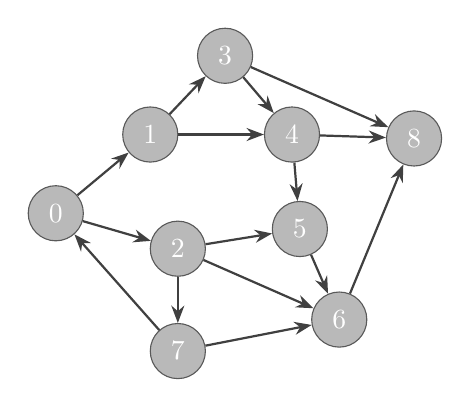
\begin{tikzpicture}[
    v/.style={circle,draw=black!65,fill=gray!55,text=white,minimum size=7mm,inner sep=0pt},
    e/.style={-{Stealth[length=2.2mm]},line width=0.8pt,black!75}
  ]
    \node[v] (v0) at (0,0) {0};
    \node[v] (v1) at (1.2,1.0) {1};
    \node[v] (v2) at (1.55,-0.45) {2};
    \node[v] (v3) at (2.15,2.0) {3};
    \node[v] (v4) at (3.0,1.0) {4};
    \node[v] (v5) at (3.1,-0.2) {5};
    \node[v] (v6) at (3.6,-1.35) {6};
    \node[v] (v7) at (1.55,-1.75) {7};
    \node[v] (v8) at (4.55,0.95) {8};
    \draw[e] (v0)--(v1); \draw[e] (v0)--(v2);
    \draw[e] (v1)--(v3); \draw[e] (v1)--(v4);
    \draw[e] (v2)--(v5); \draw[e] (v2)--(v6); \draw[e] (v2)--(v7);
    \draw[e] (v3)--(v4); \draw[e] (v3)--(v8);
    \draw[e] (v4)--(v5); \draw[e] (v4)--(v8);
    \draw[e] (v5)--(v6); \draw[e] (v6)--(v8);
    \draw[e] (v7)--(v0); \draw[e] (v7)--(v6);
  \end{tikzpicture}
  \caption{含 9 个顶点和 15 条有向边的简单图示例。依据原书图 18.1 重绘}
  \label{fig:18-1}
\end{figure}

图的一种直观表示是\textbf{邻接矩阵}（adjacency matrix）。在邻接矩阵 $A$ 中，若有
一条边从源顶点 $i$ 指向目的顶点 $j$，则邻接矩阵元素 $A[i,j]$ 的值为 1；否则为 0。
图 \ref{fig:18-2} 给出了图 \ref{fig:18-1} 中简单图的邻接矩阵。由于分别存在从顶点 1
到顶点 3、从顶点 4 到顶点 5 的边，所以 $A[1,3]$ 和 $A[4,5]$ 都是 1。为使图示清楚，
矩阵中省略了值为 0 的元素；空白元素均应理解为 0。

\begin{figure}[htbp]
  \centering
  \scriptsize
  \setlength{\tabcolsep}{4.2pt}
  \renewcommand{\arraystretch}{1.15}
  \begin{tabular}{c|*{9}{c|}}
    \multicolumn{1}{c}{\raisebox{0.5ex}{源}} &
    \multicolumn{9}{c}{目的顶点 $j$}\\
    $i$ & 0&1&2&3&4&5&6&7&8\\ \hline
    0&&1&1&&&&&&\\ \hline
    1&&&&1&1&&&&\\ \hline
    2&&&&&&1&1&1&\\ \hline
    3&&&&&1&&&&1\\ \hline
    4&&&&&&1&&&1\\ \hline
    5&&&&&&&1&&\\ \hline
    6&&&&&&&&&1\\ \hline
    7&1&&&&&&1&&\\ \hline
    8&&&&&&&&&\\ \hline
  \end{tabular}
  \caption{图 \ref{fig:18-1} 中简单图的邻接矩阵表示。依据原书图 18.2 重排}
  \label{fig:18-2}
\end{figure}

若一个含 $N$ 个顶点的图是完全连通的，也就是说每个顶点都与其他所有顶点相连，那么
每个顶点应有 $N-1$ 条出边。由于没有从顶点指向自身的边，图中总计应有
$N(N-1)$ 条边。例如，若这个 9 顶点图完全连通，每个顶点应有 8 条出边，边的总数应为
72。显然，图 \ref{fig:18-1} 的连通程度低得多，每个顶点最多只有 3 条出边。这样的图称为
\textbf{稀疏连接图}（sparsely connected graph），即每个顶点的平均出边数远小于
$N-1$。

读者此时很可能已经正确地意识到：稀疏连接图应该能从稀疏矩阵表示中受益。正如第
\ref{chap:sparse-matrix} 章所见，采用矩阵的压缩表示可以大幅减少存储需求，以及在零
元素上浪费的运算。现实中的许多图确实是稀疏连接的。例如，在社交网络中，每个用户的
平均连接数远小于用户总数，因此邻接矩阵中的非零元素数远小于元素总数。

图 \ref{fig:18-3} 用 CSR、CSC 和 COO 三种存储格式表示同一个简单图。这里把行下标数组
和行偏移数组分别称为 \code{src} 和 \code{srcPtrs}，把列下标数组和列偏移数组分别称为
\code{dst} 和 \code{dstPtrs}。以 CSR 为例，第 \ref{chap:sparse-matrix} 章已经说明，
CSR 稀疏矩阵的 \code{rowPtrs} 数组中，每个行偏移都给出相应行非零元素的起始位置。
类似地，在图的 CSR 表示中，\code{srcPtrs} 数组中每个源顶点的偏移，都给出该顶点出边的
起始位置。

例如，\code{srcPtrs[3]=7} 给出原邻接矩阵第 3 行非零元素的起始位置，
\code{srcPtrs[4]=9} 则给出第 4 行非零元素的起始位置。因此，第 3 行的非零数据位于
\code{data[7]} 和 \code{data[8]}，相应的列下标（目的顶点）位于 \code{dst[7]} 和
\code{dst[8]}。这些正是离开顶点 3 的两条边的数据和列下标。之所以把列下标数组称为
\code{dst}，是因为邻接矩阵元素的列下标给出了该边的目的顶点。在本例中，以顶点 3 为
源的两条边分别指向 \code{dst[7]=4} 和 \code{dst[8]=8}。CSC 和 COO 表示与矩阵格式
之间的类似对应关系留给读者自行推导。

\begin{figure}[htbp]
  \centering
  \scriptsize
  \setlength{\tabcolsep}{2.7pt}
  \renewcommand{\arraystretch}{1.18}
  \begin{tabular}{r|*{10}{c|}}
    \multicolumn{11}{c}{\textbf{(a) CSR 表示}}\\
    \code{srcPtrs[10]}&0&2&4&7&9&11&12&13&15&15\\ \hline
  \end{tabular}
  \\[0.35em]
  \begin{tabular}{r|*{15}{c|}}
    \code{dst[15]}&1&2&3&4&5&6&7&4&8&5&8&6&8&0&6\\ \hline
    \code{data[15]}&1&1&1&1&1&1&1&1&1&1&1&1&1&1&1\\ \hline
  \end{tabular}
  \\[0.8em]
  \begin{tabular}{r|*{10}{c|}}
    \multicolumn{11}{c}{\textbf{(b) CSC 表示}}\\
    \code{dstPtrs[10]}&0&1&2&3&4&6&8&11&12&15\\ \hline
  \end{tabular}
  \\[0.35em]
  \begin{tabular}{r|*{15}{c|}}
    \code{src[15]}&7&0&0&1&1&3&2&4&2&5&7&2&3&4&6\\ \hline
    \code{data[15]}&1&1&1&1&1&1&1&1&1&1&1&1&1&1&1\\ \hline
  \end{tabular}
  \\[0.8em]
  \begin{tabular}{r|*{15}{c|}}
    \multicolumn{16}{c}{\textbf{(c) COO 表示}}\\
    \code{src[15]}&0&0&1&1&2&2&2&3&3&4&4&5&6&7&7\\ \hline
    \code{dst[15]}&1&2&3&4&5&6&7&4&8&5&8&6&8&0&6\\ \hline
    \code{data[15]}&1&1&1&1&1&1&1&1&1&1&1&1&1&1&1\\ \hline
  \end{tabular}
  \caption{邻接矩阵的三种稀疏表示：(a) CSR；(b) CSC；(c) COO。依据原书图 18.3 重排}
  \label{fig:18-3}
\end{figure}

本例中的 \code{data} 数组并非必需，因为其中所有元素都为 1，无须实际存储。我们可以
让数据成为隐式信息：只要存在一个非零元素，就直接假定它的值为 1。例如，CSR 表示的
目的数组中每出现一个列下标，就意味着存在一条边。不过在某些应用中，邻接矩阵还会保存
关于关系的附加信息，例如两个地点间的距离，或两个社交网络用户建立连接的日期；此时就
必须显式存储 \code{data} 数组。

稀疏表示可以显著节省邻接矩阵的存储空间。在本例中，假设可以省略 \code{data} 数组，
CSR 表示需要 25 个存储位置；若保存完整邻接矩阵，则需要 $9^2=81$ 个位置。现实问题中
邻接矩阵往往只有极小一部分元素非零，节省的空间会相当可观。

\noindent\textbf{译者注：}底本 PDF 的正文视觉内容为 $9^2=81$，但文本提取层把上标 2
错误地提取成了普通数字，形成“92=81”。本译稿按原页数学排版还原为 $9^2=81$。

不同图的结构可能有天壤之别。描述这些结构的一种方法，是观察每个顶点所连边数的分布，
也就是\textbf{顶点度}（vertex degree）的分布。若把道路网络表示为图，其度分布通常
比较均匀，每个顶点的平均度较低，因为每个道路交叉口（顶点）一般只连接少量道路（边）。
另一方面，在社交网络的关注关系图中，每条入边表示一次“关注”，顶点度的分布要宽得多；
度很大的顶点代表一位很受欢迎的用户。图的结构会影响具体图应用对算法的选择。

回忆第 \ref{chap:sparse-matrix} 章，每种稀疏矩阵表示对所表示数据提供的可访问性不同，
因此图的表示选择会影响图遍历算法能够方便取得哪些信息。CSR 表示便于访问给定顶点的
出边；CSC 表示便于访问给定顶点的入边；COO 表示则便于访问给定边的源顶点和目的顶点。
所以，图表示的选择与图遍历算法的选择相伴而生。本章将考察 BFS 的多种并行实现，以此
贯穿展示这一概念。

\section{广度优先搜索}
\label{sec:breadth-first-search}

\textbf{广度优先搜索}（BFS）是一种重要的图遍历计算。它常用于确定从一个顶点到图中
任意其他顶点至少需要经过多少条边。在图 \ref{fig:18-1} 的例子中，我们可能需要寻找从
顶点 0 所代表的地点到顶点 5 所代表地点的所有备选路线。观察图可知有三条可能的路径：
$0\to1\to3\to4\to5$、$0\to1\to4\to5$ 和 $0\to2\to5$，其中
$0\to2\to5$ 最短。BFS 遍历结果有多种汇总方式。其中一种是指定一个称为\textbf{根}
（root）的顶点，并用从根到该顶点至少需要经过的边数为每个顶点加上标记。BFS 的结果
也可以帮助理解图的拓扑结构。

图 \ref{fig:18-4}(a) 给出以顶点 0 为根时所需的 BFS 结果。经过一条边可以到达顶点 1
和 2，所以把它们标为第 1 层。再经过一条边，可以到达顶点 3（经顶点 1）、顶点 4
（经顶点 1）、顶点 5（经顶点 2）、顶点 6（经顶点 2）和顶点 7（经顶点 2），因此把
这些顶点标为第 2 层。最后，再经过一条边可以从顶点 3、4 或 6 到达顶点 8。

若换一个顶点作为根，BFS 的结果会大不相同。图 \ref{fig:18-4}(b) 给出以顶点 2 为根的
结果。第 1 层顶点是 5、6 和 7；第 2 层顶点是顶点 8（经顶点 6）和顶点 0（经顶点 7）；
只有顶点 1 位于第 3 层（经顶点 0）；最后，顶点 3 和 4 都位于第 4 层（均经顶点 1）。
值得注意的是，虽然新根与原根只相隔一条边，两个结果却有很大差别。

\begin{figure}[htbp]
  \centering
  \begin{tikzpicture}[
    scale=.78,transform shape,
    v/.style={circle,draw=black!55,minimum size=7mm,inner sep=0pt},
    e/.style={-{Stealth[length=2mm]},line width=.65pt,black!70},
    lab/.style={font=\scriptsize}
  ]
    \begin{scope}[xshift=-4.1cm]
      \node[v,fill=gray!55,text=white] (a0) at (0,0) {0};
      \node[v,fill=blue!35] (a1) at (1.2,1) {1}; \node[v,fill=blue!35] (a2) at (1.55,-.45) {2};
      \node[v,fill=green!35] (a3) at (2.15,2) {3}; \node[v,fill=green!35] (a4) at (3,1) {4};
      \node[v,fill=green!35] (a5) at (3.1,-.2) {5}; \node[v,fill=green!35] (a6) at (3.6,-1.35) {6};
      \node[v,fill=green!35] (a7) at (1.55,-1.75) {7}; \node[v,fill=orange!45] (a8) at (4.55,.95) {8};
      \foreach \s/\t in {a0/a1,a0/a2,a1/a3,a1/a4,a2/a5,a2/a6,a2/a7,a3/a4,a3/a8,a4/a5,a4/a8,a5/a6,a6/a8,a7/a0,a7/a6} {\draw[e] (\s)--(\t);}
      \node[lab,left] at (a0.west) {0}; \node[lab,above left] at (a1) {1}; \node[lab,above left] at (a2) {1};
      \node[lab,above] at (a3) {2}; \node[lab,above] at (a4) {2}; \node[lab,right] at (a5) {2};
      \node[lab,right] at (a6) {2}; \node[lab,below] at (a7) {2}; \node[lab,right] at (a8) {3};
      \node[font=\small] at (2.25,-2.55) {(a) 顶点 0 为根};
    \end{scope}
    \begin{scope}[xshift=3.2cm]
      \node[v,fill=green!35] (b0) at (0,0) {0};
      \node[v,fill=orange!45] (b1) at (1.2,1) {1}; \node[v,fill=gray!55,text=white] (b2) at (1.55,-.45) {2};
      \node[v,fill=pink!45] (b3) at (2.15,2) {3}; \node[v,fill=pink!45] (b4) at (3,1) {4};
      \node[v,fill=blue!35] (b5) at (3.1,-.2) {5}; \node[v,fill=blue!35] (b6) at (3.6,-1.35) {6};
      \node[v,fill=blue!35] (b7) at (1.55,-1.75) {7}; \node[v,fill=green!35] (b8) at (4.55,.95) {8};
      \foreach \s/\t in {b0/b1,b0/b2,b1/b3,b1/b4,b2/b5,b2/b6,b2/b7,b3/b4,b3/b8,b4/b5,b4/b8,b5/b6,b6/b8,b7/b0,b7/b6} {\draw[e] (\s)--(\t);}
      \node[lab,left] at (b0.west) {2}; \node[lab,above left] at (b1) {3}; \node[lab,above left] at (b2) {0};
      \node[lab,above] at (b3) {4}; \node[lab,above] at (b4) {4}; \node[lab,right] at (b5) {1};
      \node[lab,right] at (b6) {1}; \node[lab,below] at (b7) {1}; \node[lab,right] at (b8) {2};
      \node[font=\small] at (2.25,-2.55) {(b) 顶点 2 为根};
    \end{scope}
  \end{tikzpicture}
  \caption{两个不同根顶点对应的 BFS 结果。顶点旁的数字表示距根的边数（深度）。
  依据原书图 18.4 重绘}
  \label{fig:18-4}
\end{figure}

可以把 BFS 的标记过程看作构造一棵以搜索根为根节点的\textbf{BFS 树}。这棵树包含
所有已标记顶点，但只包含搜索中实际经过的、从某一层顶点指向下一层顶点的边。给所有
顶点标出层号以后，就很容易找到一条从根到任意顶点、且所经边数等于该顶点层号的路径。
例如在图 \ref{fig:18-4}(b) 中，顶点 1 被标为第 3 层，所以根（顶点 2）到顶点 1 的
最少边数为 3。若要找出具体路径，可以从目的顶点开始反向追溯到根：每一步都选择一个
层号比当前顶点少 1 的前驱。若同一层有多个前驱，可以任取一个；其中任何一个都能给出
有效解。存在多个可选前驱，也就意味着问题有多个同样好的解。本例中，从顶点 1 出发，
依次选择顶点 0、7 和 2，便得到从顶点 2 到顶点 1 的最短路径 $2\to7\to0\to1$。
当然，这要求每个顶点都带有其全部入边源顶点的列表，才能找到给定顶点的前驱。

图 \ref{fig:18-5} 展示了 BFS 在计算机辅助设计（CAD）中的一项重要应用。设计集成电路
芯片时，需要连接许多电子元件才能完成设计。这些元件的连接器称为\textbf{网络端点}
（net terminal）。图 \ref{fig:18-5}(a) 用两个圆点表示这样的端点：一个属于芯片左上部
的元件，另一个属于右下部的元件。假设设计要求连接这两个端点，就需要从第一个端点到
第二个端点布设一条给定宽度的导线。

布线软件把芯片表示为由布线块组成的网格，每个块都有可能成为导线的一部分。导线可以
沿水平方向或垂直方向延伸。例如，图中芯片下半部黑色的 J 形障碍由 21 个布线块构成，
并连接三个网络端点。一个布线块一旦成为某条导线的一部分，就不能再用于任何其他导线；
它还会阻断周围布线块。导线不能从已用块的下邻块穿到上邻块，也不能从左邻块穿到右邻块，
依此类推。形成一条导线以后，其他所有导线都必须绕开它。布线块也可能被电路元件占据，
并施加与导线占用相同的阻断约束。这正是该问题称为\textbf{迷宫布线}（maze routing）
的原因：已有电路元件和导线为尚未形成的导线构成了一座迷宫；迷宫布线软件必须在所有
既有约束下，为每条新增导线寻找路线。

\begin{figure}[htbp]
  \centering
  \begin{tikzpicture}[x=.35cm,y=.35cm]
    \begin{scope}
      \fill[green!18] (0,0) rectangle (11,9);
      \fill[green!28] (1,4) rectangle (7,8);
      \fill[yellow!24] (2,5) rectangle (6,8);
      \fill[orange!25] (3,6) rectangle (5,8);
      \fill[black!75] (7,6) rectangle (8,9); \fill[black!75] (7,6) rectangle (11,7);
      \fill[black!75] (1,3) rectangle (7,4); \fill[black!75] (5,1) rectangle (6,4);
      \fill[black!75] (2,1) rectangle (6,2);
      \draw[step=1,black!35,thin] (0,0) grid (11,9);
      \fill[brown!80] (3.5,7.5) circle (2.3pt); \fill[brown!80] (7.5,2.5) circle (2.3pt);
      \node[font=\scriptsize] at (5.5,-.8) {(a) BFS 波前};
      \node[font=\tiny,anchor=west] at (.2,8.55) {第 3 层};
      \node[font=\tiny,anchor=west] at (1.2,7.65) {第 2 层};
      \node[font=\tiny,anchor=west] at (2.2,6.75) {第 1 层};
    \end{scope}
    \begin{scope}[xshift=5cm]
      \fill[green!18] (0,0) rectangle (11,9);
      \fill[black!75] (7,6) rectangle (8,9); \fill[black!75] (7,6) rectangle (11,7);
      \fill[black!75] (1,3) rectangle (7,4); \fill[black!75] (5,1) rectangle (6,4);
      \fill[black!75] (2,1) rectangle (6,2);
      \draw[step=1,black!35,thin] (0,0) grid (11,9);
      \draw[red!75!black,line width=1.2pt] (3.5,7.5)--(.5,7.5)--(.5,2.5)--(7.5,2.5);
      \fill[brown!80] (3.5,7.5) circle (2.3pt); \fill[brown!80] (7.5,2.5) circle (2.3pt);
      \node[font=\scriptsize] at (5.5,-.8) {(b) 确定布线路径};
    \end{scope}
    \fill[brown!80] (8.5,-2.0) circle (2.3pt); \node[font=\scriptsize,anchor=west] at (9,-2) {网络端点};
    \fill[black!75] (13,-2.35) rectangle (13.8,-1.65); \node[font=\scriptsize,anchor=west] at (14.2,-2) {障碍};
  \end{tikzpicture}
  \caption{集成电路中的迷宫布线是 BFS 的一种应用：(a) 广度优先搜索；(b) 确定一条
  布线路径。依据原书图 18.5 重绘的概念示意}
  \label{fig:18-5}
\end{figure}

迷宫布线应用把芯片表示为图：布线块是顶点；从顶点 $i$ 到顶点 $j$ 的边表示导线可以
从块 $i$ 延伸到块 $j$。一个块被导线或元件占用以后，应用会把它标为障碍顶点，或者直接
从图中移除，具体取决于应用设计。图 \ref{fig:18-5} 表明，应用可以从根网络端点到目标
网络端点做 BFS，求解迷宫布线问题。搜索从根顶点开始，逐层标记顶点：不是障碍的直接
水平或垂直邻居（总共 4 个）被标为第 1 层；图中根的 4 个邻居都可到达，所以都会进入
第 1 层。第 1 层顶点中既非障碍、也未被当前搜索访问的邻居被标为第 2 层。读者可以核实，
原书图 18.5(a) 中有 4 个第 1 层顶点、8 个第 2 层顶点和 12 个第 3 层顶点，依此类推。
可以看到，BFS 实质上为每一层形成一个顶点\textbf{波前}（wavefront）。第 1 层的波前
很小，但在短短几层之内就可能迅速变得很大。

图 \ref{fig:18-5}(b) 表明，BFS 完成后，可以通过寻找从根到目标的最短路径来形成导线。
如前所述，只需从目标顶点出发，反向追溯层号比当前顶点少 1 的前驱。若有多个前驱的层号
相同，就存在多条长度相同的路线。可以设计启发式规则来选择前驱，以尽量减轻尚未布设的
导线将要面对的约束。

\section{BFS 的顶点中心并行化}
\label{sec:bfs-vertex-centric}

并行化图算法的一种自然方法，是并行地对不同顶点或不同边执行操作。事实上，许多图算法
的并行实现都可以分为\textbf{顶点中心}（vertex-centric）和\textbf{边中心}
（edge-centric）两类。顶点中心实现把线程分配给顶点，让每个线程对自己的顶点执行操作，
通常需要遍历该顶点的邻居。算法不同，所关注的邻居可能是经出边可达的顶点、经入边可达
的顶点，或者两者兼有。与之相对，边中心实现把线程分配给边，让每个线程对自己的边执行
操作，通常需要查找该边的源顶点和目的顶点。本节考察 BFS 的两种顶点中心并行实现：一种
遍历出边，另一种遍历入边。第 \ref{sec:bfs-edge-centric} 节将考察边中心实现并加以比较。

下面各并行实现在逐层迭代时采用相同策略。所有实现都先把根顶点标为第 0 层，然后调用
一个内核，把根的全部邻居标为第 1 层；接着调用内核，把第 1 层顶点中尚未访问的邻居
标为第 2 层；再调用内核，把第 2 层顶点中尚未访问的邻居标为第 3 层。这个过程一直持续，
直到不再访问和标记任何新顶点。

每一层都要单独调用一次内核，是因为必须等上一层的全部顶点标记完毕，才能继续标记下一层，
否则可能给顶点标上错误的层号。本节余下部分聚焦于每层调用一次的这个内核：给定当前层，
它根据此前各层顶点的标记，为属于当前层的全部顶点加上标记。第
\ref{sec:bfs-cooperative-groups} 节将修改这种方法，在一次内核调用中迭代多个 BFS 层。

第一种顶点中心并行实现给每个顶点分配一个线程，让线程遍历该顶点的出边。线程先检查
自己的顶点是否属于上一层；若是，就遍历出边，把所有尚未访问的邻居标为当前层。这种
顶点中心实现通常称为\textbf{自顶向下}（top-down）或\textbf{推送式}（push）实现。
\footnote{若正在构造 BFS 树，这种实现可以看成把线程分配给 BFS 树中的父顶点，让它们
寻找自己的子顶点，因而得名“自顶向下”。这种说法假定树根在上、叶节点在下。“推送”
则是指每个活动顶点沿出边把自己的深度推送给全部邻居。}它要求能够访问给定源顶点的
出边，也就是邻接矩阵给定行中的非零元素，因此需要 CSR 表示。

图 \ref{fig:18-6} 给出顶点中心推送式内核，图 \ref{fig:18-7} 则展示该内核如何从第 1 层
（上一层）遍历到第 2 层（当前层）。内核先给每个顶点分配一个线程（第 3 行），每个线程
检查自己的顶点 ID 是否越界（第 4 行），然后检查该顶点是否属于上一层（第 5 行）。在
图 \ref{fig:18-7} 中，只有分配到顶点 1 和 2 的线程通过这项检查。这些线程随后用 CSR 的
\code{srcPtrs} 数组定位顶点的出边并逐条遍历（第 6--7 行）。对每条出边，线程用 CSR 的
\code{dst} 数组找到边的目的邻居（第 8 行），再检查该邻居是否尚未访问（第 9 行）。

\begin{figure}[htbp]
  \centering
  \begin{minipage}{0.98\textwidth}
  \begin{lstlisting}[language=C++,basicstyle=\ttfamily\scriptsize,firstnumber=1,lastline=16]
__global__ void bfs_kernel(CSRGraph csrGraph, unsigned int* level,
                           unsigned int* newVertexVisited, unsigned int currLevel) {
  unsigned int vertex = blockIdx.x*blockDim.x + threadIdx.x;
  if(vertex < csrGraph.numVertices) {
    if(level[vertex] == currLevel - 1) {
      for(unsigned int edge = csrGraph.srcPtrs[vertex];
                       edge < csrGraph.srcPtrs[vertex + 1]; ++edge) {
        unsigned int neighbor = csrGraph.dst[edge];
        if(level[neighbor] == UNVISITED) {
          level[neighbor] = currLevel;
          *newVertexVisited = 1;
        }
      }
    }
  }
}
  \end{lstlisting}
  \end{minipage}
  \caption{顶点中心推送式（自顶向下）BFS 内核。依据原书图 18.6 逐字符重排}
  \label{fig:18-6}
\end{figure}

为完成“尚未访问”的检查，所有顶点的层号起初都设为特殊值 \code{UNVISITED}。例如，
可以把它设为无符号整数的最大可能值：
\begin{lstlisting}[language=C++,numbers=none]
cuda::std::numeric_limits<unsigned>::max()
\end{lstlisting}
因此，只要邻居的层号仍为
\code{UNVISITED}，线程就知道它尚未访问。线程将未访问邻居标为当前层（第 10 行）；
成功标记一个顶点后，再设置一个标志，表明已经访问了新顶点（第 11 行）。启动代码借助
这个标志判断是需要为下一层启动新网格，还是已经抵达搜索终点。

\begin{figure}[htbp]
  \centering
  \begin{tikzpicture}[
    scale=.9,transform shape,
    v/.style={circle,draw=black!55,minimum size=7mm,inner sep=0pt},
    e/.style={-{Stealth[length=2mm]},line width=.55pt,gray!60},
    active/.style={-{Stealth[length=2.2mm]},line width=1.2pt,blue!70!black}
  ]
    \node[v,fill=gray!55,text=white] (v0) at (0,0) {0};
    \node[v,fill=blue!35] (v1) at (1.2,1) {1}; \node[v,fill=blue!35] (v2) at (1.55,-.45) {2};
    \node[v,fill=green!35] (v3) at (2.15,2) {3}; \node[v,fill=green!35] (v4) at (3,1) {4};
    \node[v,fill=green!35] (v5) at (3.1,-.2) {5}; \node[v,fill=green!35] (v6) at (3.6,-1.35) {6};
    \node[v,fill=green!35] (v7) at (1.55,-1.75) {7}; \node[v,fill=orange!45] (v8) at (4.55,.95) {8};
    \foreach \s/\t in {v0/v1,v0/v2,v3/v4,v3/v8,v4/v5,v4/v8,v5/v6,v6/v8,v7/v0,v7/v6} {\draw[e] (\s)--(\t);}
    \foreach \s/\t in {v1/v3,v1/v4,v2/v5,v2/v6,v2/v7} {\draw[active] (\s)--(\t);}
    \node[draw=blue!70!black,rounded corners=1pt,align=left,font=\scriptsize,anchor=west] at (5.3,.2)
      {活动线程：顶点 1、2\\遍历出边并标记邻居};
  \end{tikzpicture}
  \caption{顶点中心推送式 BFS 从第 1 层遍历到第 2 层的示例。蓝色粗边表示活动线程
  遍历的出边。依据原书图 18.7 重绘}
  \label{fig:18-7}
\end{figure}

请注意，多个线程可能把同一个顶点标为当前层，也可能有多个线程把标志写成 1。从技术上
说，这两种情形都是竞态条件：多个线程无序地访问同一内存位置，且其中至少一次访问是写。
正如第 14 章所讨论的，这类竞态在实践中通常是良性的，因为操作具有\textbf{幂等性}
（idempotence），执行多少次效果都相同。不过，这段代码即使实践中可以工作，仍违反了
C++ 内存模型，因而不受标准保证。采取保守做法的程序员应当对这两项操作使用原子操作。

第二种顶点中心并行实现同样给每个顶点分配一个线程，但让线程遍历该顶点的入边。线程
先检查自己的顶点是否已被访问；若尚未访问，就遍历入边，查找是否有邻居属于上一层。
只要找到一个属于上一层的邻居，线程就把自己的顶点标为当前层。这种实现通常称为
\textbf{自底向上}（bottom-up）或\textbf{拉取式}（pull）实现。\footnote{若正在构造
BFS 树，这种实现可以看成把线程分配给 BFS 树中的潜在子顶点，让它们寻找自己的父顶点，
因而得名“自底向上”。“拉取”则是指每个顶点回看其前驱，从中拉取活动状态。}它要求能够
访问给定目的顶点的入边，也就是邻接矩阵给定列中的非零元素，因此需要 CSC 表示。

\begin{figure}[htbp]
  \centering
  \begin{minipage}{0.98\textwidth}
  \begin{lstlisting}[language=C++,basicstyle=\ttfamily\scriptsize,firstnumber=1,lastline=17]
__global__ void bfs_kernel(CSCGraph cscGraph, unsigned int* level,
                           unsigned int* newVertexVisited, unsigned int currLevel) {
  unsigned int vertex = blockIdx.x*blockDim.x + threadIdx.x;
  if(vertex < cscGraph.numVertices) {
    if(level[vertex] == UNVISITED) {
      for(unsigned int edge = cscGraph.dstPtrs[vertex];
                       edge < cscGraph.dstPtrs[vertex + 1]; ++edge) {
        unsigned int neighbor = cscGraph.src[edge];
        if(level[neighbor] == currLevel - 1) {
          level[vertex] = currLevel;
          *newVertexVisited = 1;
          break;
        }
      }
    }
  }
}
  \end{lstlisting}
  \end{minipage}
  \caption{顶点中心拉取式（自底向上）BFS 内核。依据原书图 18.8 逐字符重排}
  \label{fig:18-8}
\end{figure}

图 \ref{fig:18-8} 给出拉取式内核，图 \ref{fig:18-9} 展示它如何从第 1 层遍历到第 2 层。
内核先给每个顶点分配线程（第 3 行）并做边界检查（第 4 行），然后检查自己的顶点是否
尚未访问（第 5 行）。图 \ref{fig:18-9} 中，分配到顶点 3--8 的线程都通过这项检查。
它们用 CSC 的 \code{dstPtrs} 数组定位顶点的入边并逐条遍历（第 6--7 行），再用 CSC 的
\code{src} 数组找到每条入边源端的邻居（第 8 行）。线程检查该邻居是否属于上一层
（第 9 行）；若是，就把自己的顶点标为当前层（第 10 行），设置新顶点访问标志（第 11 行），
并跳出循环（第 12 行）。

\begin{figure}[htbp]
  \centering
  \begin{tikzpicture}[
    scale=.9,transform shape,
    v/.style={circle,draw=black!55,minimum size=7mm,inner sep=0pt},
    e/.style={-{Stealth[length=2mm]},line width=.55pt,gray!60},
    hit/.style={-{Stealth[length=2.2mm]},line width=1.2pt,green!55!black},
    miss/.style={-{Stealth[length=2mm]},line width=1pt,dashed,orange!80!black}
  ]
    \node[v,fill=gray!55,text=white] (v0) at (0,0) {0};
    \node[v,fill=blue!35] (v1) at (1.2,1) {1}; \node[v,fill=blue!35] (v2) at (1.55,-.45) {2};
    \node[v,fill=green!35] (v3) at (2.15,2) {3}; \node[v,fill=green!35] (v4) at (3,1) {4};
    \node[v,fill=green!35] (v5) at (3.1,-.2) {5}; \node[v,fill=green!35] (v6) at (3.6,-1.35) {6};
    \node[v,fill=green!35] (v7) at (1.55,-1.75) {7}; \node[v,fill=orange!45] (v8) at (4.55,.95) {8};
    \foreach \s/\t in {v0/v1,v0/v2,v3/v4,v3/v8,v4/v5,v4/v8,v5/v6,v6/v8,v7/v0,v7/v6} {\draw[e] (\s)--(\t);}
    \foreach \s/\t in {v1/v3,v1/v4,v2/v5,v2/v6,v2/v7} {\draw[hit] (\s)--(\t);}
    \draw[miss] (v6)--(v8);
    \node[draw=green!55!black,align=left,font=\scriptsize,anchor=west] at (5.3,.35)
      {顶点 3--7 找到上一层入邻居\\并标记自身};
    \node[draw=orange!80!black,align=left,font=\scriptsize,anchor=west] at (5.3,-.75)
      {顶点 8 检查全部入边\\但尚不能标记};
  \end{tikzpicture}
  \caption{顶点中心拉取式遍历从第 1 层到第 2 层的示例。依据原书图 18.9 重绘}
  \label{fig:18-9}
\end{figure}

之所以可以跳出循环，是因为线程只要确认自己的顶点有一个邻居位于上一层，就足以证明
自己的顶点位于当前层，无须继续检查其余邻居。只有那些没有任何上一层邻居的顶点所对应
的线程，才会完整遍历邻居列表。在图 \ref{fig:18-9} 中，只有分配到顶点 8 的线程没有
提前跳出，而是遍历完整个邻居列表。

比较推送式和拉取式顶点中心实现时，有两个对性能影响很大的关键区别。第一个区别是，
推送式实现中的线程会遍历其顶点的完整邻居列表，而拉取式实现中的线程可能提前跳出循环。
对道路网络或 CAD 电路模型这类低顶点度、低方差的图而言，邻居列表很短、长度也相近，
这项差异可能并不重要。但对社交网络这类高顶点度、高方差的图而言，邻居列表很长，长度
也可能相差悬殊，造成严重负载不均衡和线程间控制流分歧。此时，提前跳出循环能够减少
负载不均衡与控制流分歧，带来显著的性能收益。

第二个重要区别是：推送式实现中，只有分配到上一层顶点的线程才遍历邻居列表；拉取式
实现中，分配到任意未访问顶点的线程都会遍历邻居列表。在搜索前期，每层顶点数通常较少，
而图中未访问顶点很多，所以推送式实现遍历的邻居列表更少，性能通常更好。到了搜索后期，
每层顶点数通常更多，未访问顶点则更少；此外，拉取式实现找到已访问邻居并提前跳出的概率
也更高，因此后期通常是拉取式实现表现更好。

据此，一项常见优化是前期采用推送式实现，后期切换到拉取式实现。这通常称为
\textbf{方向优化}（direction optimization）实现。何时切换通常取决于图的类型。平均
顶点度和方差较低的图通常层数很多，需要经过较长时间，才会出现单层顶点很多且相当一部分
顶点已经访问的局面。相反，平均顶点度和方差较高的图通常层数较少，各层规模增长很快。
这类只经过几层就能从任意顶点抵达其他顶点的图，通常称为\textbf{小世界图}
（small-world graph）。因此，高平均顶点度图从推送式切换到拉取式的时机，通常远早于
低平均顶点度图。

推送式实现使用图的 CSR 表示，拉取式实现则使用 CSC 表示。因此，若采用方向优化实现，
就需要同时保存图的 CSR 和 CSC 表示。在社交网络或迷宫布线等许多应用中，图是无向的，
这意味着邻接矩阵对称。此时 CSR 和 CSC 表示等价，只需保存一份，供两种实现共同使用。

\section{BFS 的边中心并行化}
\label{sec:bfs-edge-centric}

现在考察 BFS 的一种边中心并行实现。每个线程分配到一条边，检查边的源顶点是否属于
上一层、目的顶点是否尚未访问；若两项条件都满足，就把未访问的目的顶点标为当前层。
这种实现需要能够访问给定边的源顶点和目的顶点，也就是给定非零元素的行、列下标，因此
需要 COO 数据结构。

\begin{figure}[htbp]
  \centering
  \begin{minipage}{0.98\textwidth}
  \begin{lstlisting}[language=C++,basicstyle=\ttfamily\scriptsize,firstnumber=1,lastline=14]
__global__ void bfs_kernel(COOGraph cooGraph, unsigned int* level,
                           unsigned int* newVertexVisited, unsigned int currLevel) {
  unsigned int edge = blockIdx.x*blockDim.x + threadIdx.x;
  if(edge < cooGraph.numEdges) {
    unsigned int vertex = cooGraph.src[edge];
    if(level[vertex] == currLevel - 1) {
      unsigned int neighbor = cooGraph.dst[edge];
      if(level[neighbor] == UNVISITED) {
        level[neighbor] = currLevel;
        *newVertexVisited = 1;
      }
    }
  }
}
  \end{lstlisting}
  \end{minipage}
  \caption{边中心 BFS 内核。依据原书图 18.10 逐字符重排}
  \label{fig:18-10}
\end{figure}

图 \ref{fig:18-10} 给出边中心内核，图 \ref{fig:18-11} 展示该内核如何从第 1 层遍历到
第 2 层。内核先给每条边分配一个线程（第 3 行）并检查边 ID 是否越界（第 4 行）。
线程用 COO 的 \code{src} 数组找到边的源顶点（第 5 行），并检查它是否属于上一层
（第 6 行）。图 \ref{fig:18-11} 中，只有分配到顶点 1 和 2 出边的线程通过检查。这些
线程用 COO 的 \code{dst} 数组定位边的目的邻居（第 7 行），并检查邻居是否尚未访问
（第 8 行）；若是，就把它标为当前层（第 9 行），最后设置新顶点访问标志（第 10 行）。

\begin{figure}[htbp]
  \centering
  \begin{tikzpicture}[
    scale=.9,transform shape,
    v/.style={circle,draw=black!55,minimum size=7mm,inner sep=0pt},
    e/.style={-{Stealth[length=2mm]},line width=.55pt,gray!55},
    active/.style={-{Stealth[length=2.2mm]},line width=1.2pt,purple!75!black}
  ]
    \node[v,fill=gray!55,text=white] (v0) at (0,0) {0};
    \node[v,fill=blue!35] (v1) at (1.2,1) {1}; \node[v,fill=blue!35] (v2) at (1.55,-.45) {2};
    \node[v,fill=green!35] (v3) at (2.15,2) {3}; \node[v,fill=green!35] (v4) at (3,1) {4};
    \node[v,fill=green!35] (v5) at (3.1,-.2) {5}; \node[v,fill=green!35] (v6) at (3.6,-1.35) {6};
    \node[v,fill=green!35] (v7) at (1.55,-1.75) {7}; \node[v,fill=orange!45] (v8) at (4.55,.95) {8};
    \foreach \s/\t in {v0/v1,v0/v2,v3/v4,v3/v8,v4/v5,v4/v8,v5/v6,v6/v8,v7/v0,v7/v6} {\draw[e] (\s)--(\t);}
    \foreach \s/\t in {v1/v3,v1/v4,v2/v5,v2/v6,v2/v7} {\draw[active] (\s)--(\t);}
    \node[draw=purple!75!black,align=left,font=\scriptsize,anchor=west] at (5.3,.15)
      {每条边一个线程\\紫色边对应线程执行遍历};
  \end{tikzpicture}
  \caption{边中心实现从第 1 层遍历到第 2 层的示例。依据原书图 18.11 重绘}
  \label{fig:18-11}
\end{figure}

相对顶点中心实现，边中心实现有两项主要优势。第一，它暴露的并行度更高。顶点中心实现
面对顶点数很少的图时，可能无法启动足够多的线程来充分占用设备。图中的边通常远多于
顶点，所以边中心实现可以启动更多线程，通常更适合小图。

第二，边中心实现的负载不均衡和控制流分歧更少。在顶点中心实现中，每个线程遍历多少条
边取决于分配到的顶点度；边中心实现中，每个线程只遍历一条边。相对于顶点中心实现，
边中心实现正是第 6 章所讨论的“重新安排线程到工作/数据的映射以减少控制流分歧”的一个
例子。它通常更适合平均顶点度较高、且各顶点度差异很大的图。

边中心实现的缺点是必须检查图中的每一条边。顶点中心实现若判断一个顶点与当前层无关，
就可以跳过整张边列表。例如，设顶点 $v$ 有 $n$ 条边，却与某一层无关。边中心实现会为
这 $n$ 条边分别启动线程，每个线程都独立检查 $v$，然后发现自己的边无关；顶点中心实现
只需为 $v$ 启动一个线程，检查一次 $v$ 后便跳过全部 $n$ 条边。边中心实现的另一项缺点
是采用 COO；与顶点中心实现采用的 CSR 和 CSC 相比，COO 需要更多空间来存边。

读者也许已经发现，本节和上一节的代码示例与第 \ref{chap:sparse-matrix} 章的 SpMV 实现
很相似。事实上，只要略作调整，就可以把一次 BFS 层迭代完全表示成 SpMV 和少量其他向量
操作，其中 SpMV 是主导操作。除 BFS 外，许多其他图计算也可以用邻接矩阵上的稀疏矩阵
运算来表述\cite{kepner2011graph}。这通常称为图问题的\textbf{线性代数表述}
（linear algebraic formulation），也是 GraphBLAS API 规范\cite{davis2019graphblas}
关注的核心。线性代数表述的优势是可以利用成熟且高度优化的并行稀疏线性代数库来完成
图计算；缺点则是可能错过利用特定图算法性质的优化机会。

\section{用前沿提高工作效率}
\label{sec:bfs-frontiers}

前两节的方法在每次迭代中，都要检查每个顶点或每条边是否与当前层有关。这种策略的
优点是内核并行度很高，不要求线程间同步；缺点则是每次迭代都会启动许多不必要的线程，
执行大量无效工作，因此不具备工作效率。例如在顶点中心实现中，要为图中每个顶点启动
线程，其中许多线程只是发现顶点无关，根本不做实际工作；边中心实现同样要为每条边启动
线程，其中许多线程只是发现边无关，没有完成任何有用工作。

为了量化这些方法的工作效率，考虑一个含 $n$ 个顶点、$m$ 条边、直径为 $d$ 的图；这里
$d$ 指不含第 0 层在内的 BFS 层数。理想情况下，每个顶点和每条边都只访问一次，所以
BFS 的理想\textbf{工作复杂度}（work complexity）为 $O(n+m)$。顶点中心推送式方法在
每一层检查每个顶点，但只有当源顶点属于上一层时才会遍历相应边，所以工作复杂度为
$O(d\,n+m)$。顶点中心拉取式方法不仅在每一层检查每个顶点，而且只要目的顶点尚未访问，
每条边也可能在到达最后一层之前被多个层反复检查，所以工作复杂度为 $O(d\,n+d\,m)$。
边中心方法在每一层检查每条边，工作复杂度为 $O(d\,m)$。这些工作复杂度没有一个达到
理想值，说明上述实现都不具备工作效率。

\noindent\textbf{译者注：}底本在拉取式复杂度 $O(d\,n+d\,m)$ 后多印了一个右括号。
本译稿删除该多余括号，只修正数学定界，不改变公式含义。

本节要避免启动不必要的线程，并消除这些线程在每次迭代中的冗余检查，从而提高并行 BFS
的工作效率。下面聚焦第 \ref{sec:bfs-vertex-centric} 节的顶点中心推送式方法。该方法
每一层都为图中的每个顶点启动一个线程；线程检查自己的顶点是否属于上一层，若是，就把
所有尚未访问的邻居标为当前层；不属于上一层的顶点所对应的线程则什么也不做。理想情况下，
这些线程根本不该启动。为了避免启动它们，可以让处理上一层顶点的线程协作构造一个
\textbf{前沿}（frontier），其中保存这些线程新访问的顶点。处理当前层时，只需为这个
前沿中的顶点启动线程\cite{luo2010bfs}。这样，每个顶点只检查一次，每条边只遍历一次，
工作复杂度恢复为 $O(n+m)$。

\noindent\textbf{译者注：}底本在上述回顾中写成“不在当前层的顶点所对应的线程不做
任何事”，但该实现实际检查的是顶点是否属于\emph{上一层}，图 18.6 第 5 行及相邻句也
都如此。本译稿按代码与上下文最小修正为“上一层”。

\begin{figure}[htbp]
  \centering
  \begin{minipage}{0.98\textwidth}
  \begin{lstlisting}[language=C++,basicstyle=\ttfamily\scriptsize,firstnumber=1,lastline=20]
__global__ void bfs_kernel(CSRGraph csrGraph, unsigned int* level,
                           unsigned int* prevFrontier, unsigned int* currFrontier,
                           unsigned int numPrevFrontier, unsigned int* numCurrFrontier,
                           unsigned int currLevel) {
  unsigned int i = blockIdx.x*blockDim.x + threadIdx.x;
  if(i < numPrevFrontier) {
    unsigned int vertex = prevFrontier[i];
    for(unsigned int edge = csrGraph.srcPtrs[vertex];
                     edge < csrGraph.srcPtrs[vertex + 1]; ++edge) {
      unsigned int neighbor = csrGraph.dst[edge];
      if(visitVertexAtomically(neighbor, level, currLevel)) {
        cuda::atomic_ref<unsigned int, cuda::thread_scope_device>
            numCurrFrontier_ref(*numCurrFrontier);
        unsigned int currFrontierIdx =
            numCurrFrontier_ref.fetch_add(1, cuda::memory_order_relaxed);
        currFrontier[currFrontierIdx] = neighbor;
      }
    }
  }
}
  \end{lstlisting}
  \end{minipage}
  \caption{带前沿的顶点中心推送式（自顶向下）BFS 内核。依据原书图 18.12 逐字符重排}
  \label{fig:18-12}
\end{figure}

图 \ref{fig:18-12} 给出使用前沿的顶点中心推送式内核，图 \ref{fig:18-13} 展示它如何
从第 1 层遍历到第 2 层。与此前方法的一项关键区别是，内核增加了表示前沿的参数：数组
\code{prevFrontier} 保存上一前沿中的顶点，\code{currFrontier} 保存当前前沿中的顶点。
\code{numPrevFrontier} 保存上一前沿的顶点数，\code{numCurrFrontier} 保存当前前沿的
顶点数。用于表明
已访问新顶点的标志不再需要；当前前沿中的顶点数为 0 时，主机就知道搜索已经结束。

内核先为上一前沿的每个元素分配一个线程（第 5 行），并由线程检查元素 ID 是否越界
（第 6 行）。图 \ref{fig:18-13} 中，上一前沿只含顶点 1 和 2，所以只需启动两个线程。
每个线程从上一前沿加载一个元素，也就是自己负责的顶点下标（第 7 行），用 CSR 的
\code{srcPtrs} 数组定位顶点的出边并逐条遍历（第 8--9 行），再用 CSR 的 \code{dst}
数组找到边的目的邻居（第 10 行）。随后线程调用设备函数
\code{visitVertexAtomically}，检查邻居是否尚未访问；若是，就把邻居标为当前层
（第 11 行）。该函数的实现稍后讨论。

\begin{figure}[htbp]
  \centering
  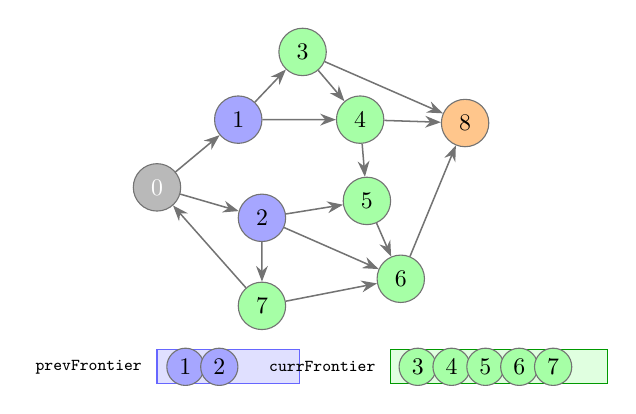
\begin{tikzpicture}[
    scale=.86,transform shape,
    v/.style={circle,draw=black!55,minimum size=7mm,inner sep=0pt},
    e/.style={-{Stealth[length=2mm]},line width=.55pt,black!55}
  ]
    \node[v,fill=gray!55,text=white] (v0) at (0,0) {0};
    \node[v,fill=blue!35] (v1) at (1.2,1) {1}; \node[v,fill=blue!35] (v2) at (1.55,-.45) {2};
    \node[v,fill=green!35] (v3) at (2.15,2) {3}; \node[v,fill=green!35] (v4) at (3,1) {4};
    \node[v,fill=green!35] (v5) at (3.1,-.2) {5}; \node[v,fill=green!35] (v6) at (3.6,-1.35) {6};
    \node[v,fill=green!35] (v7) at (1.55,-1.75) {7}; \node[v,fill=orange!45] (v8) at (4.55,.95) {8};
    \foreach \s/\t in {v0/v1,v0/v2,v1/v3,v1/v4,v2/v5,v2/v6,v2/v7,v3/v4,v3/v8,v4/v5,v4/v8,v5/v6,v6/v8,v7/v0,v7/v6} {\draw[e] (\s)--(\t);}
    \node[font=\scriptsize,anchor=east] at (-.1,-2.65) {\code{prevFrontier}};
    \draw[fill=blue!12,draw=blue!60] (0,-2.9) rectangle (2.1,-2.4);
    \node[v,fill=blue!35,minimum size=5.5mm] at (.42,-2.65) {1};
    \node[v,fill=blue!35,minimum size=5.5mm] at (.92,-2.65) {2};
    \node[font=\scriptsize,anchor=east] at (3.35,-2.65) {\code{currFrontier}};
    \draw[fill=green!12,draw=green!60!black] (3.45,-2.9) rectangle (6.65,-2.4);
    \foreach \x/\n in {3.85/3,4.35/4,4.85/5,5.35/6,5.85/7} {\node[v,fill=green!35,minimum size=5.5mm] at (\x,-2.65) {\n};}
  \end{tikzpicture}
  \caption{带前沿的顶点中心推送式 BFS 从第 1 层遍历到第 2 层的示例。依据原书
  图 18.13 重绘}
  \label{fig:18-13}
\end{figure}

若函数返回成功标记邻居，线程就必须把该邻居加入当前前沿。为此，线程以原子方式递增
当前前沿的大小（第 12--15 行），并把邻居插入对应位置（第 16 行）。多个线程可能同时
递增前沿大小，所以这个递增必须是原子的，否则会发生竞态条件。

现在来看第 11 行调用的 \code{visitVertexAtomically} 设备函数。线程遍历自己顶点的邻居
时，会检查邻居是否已访问；若没有，就把它标为当前层。不带前沿的顶点中心推送式内核
（图 \ref{fig:18-6} 第 9--10 行）没有使用原子操作来完成检查和标记。若多个线程在其中
任何一个写入新标记之前，都读到同一邻居的旧标记，那么多个线程最终可能重复标记该邻居。
由于所有线程写入的标记相同，这项操作是幂等的，允许冗余标记不会影响遍历结果。

\noindent\textbf{译者注：}底本把上一段“不带前沿的”推送式内核误指为图 18.12；
图 18.12 明明正是带前沿版本。结合“不使用原子操作”和“第 9--10 行”两项描述，实际
所指应是图 18.6。本译稿把正文引用最小修正为图 \ref{fig:18-6}。

相比之下，图 \ref{fig:18-12} 的前沿实现不仅标记未访问邻居，还把它加入前沿。如果
多个线程都观察到该邻居尚未访问，它们就会把同一邻居多次加入前沿。这样，下一层会多次
处理该邻居，造成冗余和浪费。

要避免多个线程同时观察到“尚未访问”，就必须以原子方式检查并更新邻居的标记。换句话说，
“检查邻居尚未访问”和“若是则标为当前层”必须合并到一次原子操作中。能够完成这两个步骤
的操作是\textbf{比较并交换}（compare-and-swap），C++ 通过函数
\code{compare_exchange_strong} 提供该操作。设备函数 \code{visitVertexAtomically}
正是用这个 C++ 函数访问顶点。

\begin{figure}[htbp]
  \centering
  \begin{minipage}{0.98\textwidth}
  \begin{lstlisting}[language=C++,basicstyle=\ttfamily\scriptsize,firstnumber=1,lastline=9]
__device__ inline unsigned int visitVertexAtomically(unsigned int vertex,
                                                     unsigned int* level, unsigned int currLevel) {
  cuda::atomic_ref<unsigned int, cuda::thread_scope_device>
      level_ref(level[vertex]);
  unsigned int unvisited = UNVISITED;
  unsigned int visitSuccess = level_ref.compare_exchange_strong(unvisited,
      currLevel, cuda::memory_order_relaxed, cuda::memory_order_relaxed);
  return visitSuccess;
}
  \end{lstlisting}
  \end{minipage}
  \caption{使用原子比较并交换操作来原子地访问顶点的设备函数。依据原书图 18.14
  逐字符重排}
  \label{fig:18-14}
\end{figure}

图 \ref{fig:18-14} 给出该设备函数的实现。首先为待访问顶点的层号
\code{level[vertex]} 创建原子引用（第 3--4 行）。然后通过这个引用调用
\code{compare_exchange_strong}，以原子方式更新层号（第 6--7 行）。
该函数接受 4 个参数。第一个是要与所引用数据比较的值。本例要把 \code{level[vertex]}
与 \code{UNVISITED} 比较，检查顶点是否尚未访问。但 \code{UNVISITED} 是常量，而函数
要求取得对象的引用，不能直接传入。因此代码创建整数 \code{unvisited}，用常量
\code{UNVISITED} 初始化（第 5 行），再把该整数作为第一个参数传入（第 6 行）。第二个
参数是在比较成功时写入所引用数据的值；本例希望把 \code{level[vertex]} 设为当前层，
所以传入 \code{currLevel}（第 7 行）。

第三、第四个参数分别规定原子操作成功与失败时，其内存访问的顺序要求。本例中的原子操作
不必相对于内核执行的其他独立内存访问形成特定顺序，所以两种情形都选择
\code{cuda::memory_order_relaxed}（第 7 行）。\code{compare_exchange_strong} 的
返回值表明交换是否成功；函数把该值作为设备函数结果返回（第 8 行），从而指出顶点层号
是否已成功更新。

如前所述，基于前沿的方法只为相关顶点启动线程，减少了冗余工作，这是它相对上一节方法
的优势。它的缺点则是高延迟原子操作的开销，尤其是多个原子操作争用同一数据时。更新
顶点层号的比较并交换预计只有中等程度的争用，因为只有一部分线程会访问同一个未访问
邻居；用于递增前沿大小的原子加法则预计会有严重争用，因为所有线程都递增同一个计数器，
以便向同一个前沿加入顶点。下一节将说明如何降低这种争用。

\section{用私有化减少争用}
\label{sec:bfs-privatization}

不同线程向前沿插入元素的模式，应该会让读者想起第 12 章介绍的不稳定过滤模式。在不稳定
过滤中，我们用两种优化来减少原子操作的争用：合并原子操作和私有化。这两种优化同样
适用于基于前沿的 BFS 内核。正如第 12 章所述，可以假定编译器会合并原子操作；本节重点
讨论如何利用私有化，在向当前迭代的前沿加入顶点时减少原子操作争用。

回忆第 6 章，\textbf{私有化}通过先把局部更新应用到数据的私有副本，再在完成后更新
公共副本，从而减少原子操作争用。可以把私有化用于并发前沿更新，也就是对
\code{numCurrFrontier} 的递增：让每个线程块在计算过程中维护自己的私有前沿，完成后
再更新公共前沿。这样，线程只会与同一线程块中的其他线程争用同一份数据。私有前沿及其
计数器还可以存放在共享内存中，使计数器上的原子操作和私有前沿上的存储具有更低延迟。
此外，把共享内存中的私有前沿写入全局内存中的公共前沿时，还可以合并这些内存访问。

\begin{figure}[p]
  \centering
  \begin{minipage}{0.99\textwidth}
  \begin{lstlisting}[language=C++,basicstyle=\ttfamily\fontsize{5.5pt}{6pt}\selectfont,
    numberstyle=\fontsize{5pt}{6pt}\selectfont\color{gray},aboveskip=0pt,belowskip=0pt,
    firstnumber=1,lastline=58]
__global__ void bfs_kernel(CSRGraph csrGraph, unsigned int* level,
                           unsigned int* prevFrontier, unsigned int* currFrontier,
                           unsigned int numPrevFrontier, unsigned int* numCurrFrontier,
                           unsigned int currLevel) {

  // Initialize private frontier
  __shared__ unsigned int currFrontier_s[PRIVATE_FRONTIER_CAPACITY];
  __shared__ unsigned int numCurrFrontier_s;
  if(threadIdx.x == 0) {
    numCurrFrontier_s = 0;
  }
  __syncthreads();

  // Perform BFS
  unsigned int i = blockIdx.x*blockDim.x + threadIdx.x;
  if(i < numPrevFrontier) {
    unsigned int vertex = prevFrontier[i];
    for(unsigned int edge = csrGraph.srcPtrs[vertex];
                     edge < csrGraph.srcPtrs[vertex + 1]; ++edge) {
      unsigned int neighbor = csrGraph.dst[edge];
      if(visitVertexAtomically(neighbor, level, currLevel)) {
        cuda::atomic_ref<unsigned int, cuda::thread_scope_block>
            numCurrFrontier_s_ref(numCurrFrontier_s);
        unsigned int currFrontierIdx_s =
            numCurrFrontier_s_ref.fetch_add(1, cuda::memory_order_relaxed);
        if(currFrontierIdx_s < PRIVATE_FRONTIER_CAPACITY) {
          currFrontier_s[currFrontierIdx_s] = neighbor;
        } else {
          numCurrFrontier_s = PRIVATE_FRONTIER_CAPACITY;
          cuda::atomic_ref<unsigned int, cuda::thread_scope_device>
              numCurrFrontier_ref(*numCurrFrontier);
          unsigned int currFrontierIdx =
              numCurrFrontier_ref.fetch_add(1, cuda::memory_order_relaxed);
          currFrontier[currFrontierIdx] = neighbor;
        }
      }
    }
  }
  __syncthreads();

  // Allocate in public frontier
  __shared__ unsigned int currFrontierStartIdx;
  if(threadIdx.x == 0) {
    cuda::atomic_ref<unsigned int, cuda::thread_scope_device>
        numCurrFrontier_ref(*numCurrFrontier);
    currFrontierStartIdx = numCurrFrontier_ref.fetch_add(numCurrFrontier_s,
        cuda::memory_order_relaxed);
  }
  __syncthreads();

  // Commit to public frontier
  for(unsigned int currFrontierIdx_s = threadIdx.x;
                       currFrontierIdx_s < numCurrFrontier_s; currFrontierIdx_s += blockDim.x) {
    unsigned int currFrontierIdx = currFrontierStartIdx + currFrontierIdx_s;
    currFrontier[currFrontierIdx] = currFrontier_s[currFrontierIdx_s];
  }

}
  \end{lstlisting}
  \end{minipage}
  \caption{对前沿做私有化的顶点中心推送式（自顶向下）BFS 内核。依据原书图 18.15
  逐字符重排}
  \label{fig:18-15}
\end{figure}

图 \ref{fig:18-15} 给出采用私有化前沿的顶点中心推送式内核，图 \ref{fig:18-16} 则
说明前沿如何私有化。内核首先在共享内存中为每个线程块声明一份私有前沿（第 7--8 行）。
块内的一个线程把私有前沿计数器初始化为 0（第 9--11 行），块内所有线程随后停在
\code{__syncthreads()} 屏障，等待初始化完成后再使用计数器（第 12 行）。接下来的代码
与上一版本类似：每个线程从前沿加载自己的顶点（第 17 行），遍历其出边（第 18--19 行），
找到边目的端的邻居（第 20 行），再以原子方式检查邻居是否尚未访问；若是，就访问它
（第 21 行）。

若线程成功访问了邻居，也就是说邻居此前尚未访问，就把它加入私有前沿。线程先以原子
方式递增私有前沿计数器（第 22--25 行）。若私有前沿尚未填满（第 26 行），就把邻居插入
私有前沿（第 27 行）。若私有前沿已经溢出，则把私有前沿计数器恢复到容量上限
（第 29 行），并回退到公共前沿：以原子方式递增公共前沿计数器（第 30--33 行），再把
邻居存到相应位置（第 34 行）。因此，即使共享内存私有前沿容量不足，顶点也不会丢失。

一个线程块中的全部线程遍历完各自顶点的邻居后，必须把私有前沿元素写入公共前沿。线程
先互相等待，确保不会再有邻居加入私有前沿（第 39 行）。接着由块内一个线程代表其他线程，
一次性在公共前沿中为私有前沿的全部元素分配空间（第 42--48 行），其余线程停在屏障等待
（第 49 行）。最后，线程遍历私有前沿中的顶点（第 52--53 行），把它们写入公共前沿
（第 54--55 行）。注意，公共前沿下标 \code{currFrontierIdx} 用
\code{currFrontierIdx_s} 表示，后者又由 \code{threadIdx.x} 导出。因此，线程下标
连续的线程写入连续的全局内存位置，存储访问得以合并。

\begin{figure}[htbp]
  \centering
  \resizebox{0.96\textwidth}{!}{%
  \begin{tikzpicture}[x=.72cm,y=.72cm,font=\scriptsize]
    \foreach \b/\c/\n in {0/blue/3,1/green/4,2/orange/2,3/pink/3} {
      \begin{scope}[xshift=\b*4.1cm]
        \draw[rounded corners=1pt,draw=\c!70!black,line width=.8pt] (0,1.2) rectangle (3.4,3.2);
        \foreach \x in {.55,1.25,1.95,2.65} {\draw[-{Stealth[length=1.6mm]},black!70] (\x,2.9)--(\x,1.55);}
        \node at (1.7,1.0) {\code{numCurrFrontier_s}};
        \foreach \i in {0,...,5} {\draw (0.2+\i*.5,0) rectangle +(0.5,.45);}
        \foreach \i in {1,...,\n} {\fill[\c!45] ({0.2+(\i-1)*.5},0) rectangle +(0.5,.45);}
        \node[anchor=east] at (.05,.22) {\code{currFrontier_s}};
      \end{scope}
    }
    \draw[-{Stealth[length=2.2mm]},blue!70!black,line width=1pt] (1.7,-.15)--(4.2,-1.4);
    \draw[-{Stealth[length=2.2mm]},green!60!black,line width=1pt] (5.8,-.15)--(10.4,-1.4);
    \draw[-{Stealth[length=2.2mm]},orange!80!black,line width=1pt] (9.9,-.15)--(7.0,-1.4);
    \draw[-{Stealth[length=2.2mm]},pink!75!black,line width=1pt] (14.0,-.15)--(8.7,-1.4);
    \node[anchor=east] at (3.2,-1.65) {公共 \code{currFrontier}};
    \foreach \i in {0,...,11} {\draw (3.4+\i*.65,-1.9) rectangle +(0.65,.55);}
    \foreach \i in {0,1,2} {\fill[blue!45] (3.4+\i*.65,-1.9) rectangle +(0.65,.55);}
    \foreach \i in {3,4} {\fill[orange!45] (3.4+\i*.65,-1.9) rectangle +(0.65,.55);}
    \foreach \i in {5,6,7} {\fill[pink!45] (3.4+\i*.65,-1.9) rectangle +(0.65,.55);}
    \foreach \i in {8,9,10,11} {\fill[green!45] (3.4+\i*.65,-1.9) rectangle +(0.65,.55);}
    \node[anchor=west] at (11.5,-1.65) {\code{numCurrFrontier}};
  \end{tikzpicture}
  }
  \caption{前沿私有化示例：每个线程块先更新共享内存私有前沿，再把连续片段合并写入
  全局内存公共前沿。依据原书图 18.16 重绘}
  \label{fig:18-16}
\end{figure}

\section{用协作组减少启动开销}
\label{sec:bfs-cooperative-groups}

到目前为止开发的 BFS 内核需要由主机 CPU 多次调用，每个 BFS 层调用一次。处理社交网络
这类平均顶点度较高的图时，前沿很大，网格启动开销相对于网格完成的工作量可以忽略。
但处理道路网络这类平均顶点度较低的图时，前沿很小，网格启动开销就可能支配整体性能。

为了缓解多次启动网格的开销，我们希望只启动一个网格就完成全部计算。然而，这要求在
相邻层之间执行一次\textbf{网格范围屏障同步}（grid-wide barrier synchronization），
确保各线程已经找完当前层的顶点，再进入下一层。CUDA 的\textbf{协作组}
（cooperative groups）API 可以完成这种同步，但网格范围屏障同步会对网格的线程块数
施加约束。

回忆第 4 章，网格启动时的线程块数可以超过硬件能够同时执行的数量。硬件会同时调度并
执行尽可能多的线程块，等先前线程块完成后再换入新块。这种调度方法的问题在于，所有
线程块之间不能随意执行网格范围屏障同步，否则可能死锁：已调度的线程块等待未调度块
到达屏障；未调度块又等待已调度块执行完毕、腾出位置。要执行网格范围屏障同步，必须
保证参与屏障的全部线程块都已在 SM 上活动执行，从而都能到达屏障。为提供这一保证，
启动的线程块数不得超过能够同时执行的最大线程块数。

可以使用第 4 章介绍的 CUDA 占用率计算函数，求出能够同时执行的最大线程块数。具体而言，
每个 SM 能够同时执行的最大线程块数可按如下方式得到：

\begin{lstlisting}[language=C++,numbers=none]
int numBlocksPerSM;
cudaOccupancyMaxActiveBlocksPerMultiprocessor(&numBlocksPerSM,
    bfs_kernel, numThreadsPerBlock, 0);
\end{lstlisting}

\code{cudaOccupancyMaxActiveBlocksPerMultiprocessor} 的第二、第三、第四个参数分别是目标
内核 \code{bfs_kernel}、每块线程数，以及每块所需的动态共享内存量（本例为 0）。它
计算每个 SM 可以同时执行的最大线程块数，并把结果写入第一个参数所指的
\code{numBlocksPerSM}。

知道每个 SM 能同时执行的最大线程块数以后，还需要知道目标 GPU 的 SM 数量，才能求出
整个设备可以同时执行的最大线程块总数。正如第 4 章所述，可以通过查询设备属性取得
SM 数量：

\begin{lstlisting}[language=C++,numbers=none]
cudaDeviceProp deviceProp;
cudaGetDeviceProperties(&deviceProp, 0);
int numSMs = deviceProp.multiProcessorCount;
\end{lstlisting}

再把每个 SM 的最大线程块数乘以 SM 数量，得到能够同时运行的最大线程块总数：

\begin{lstlisting}[language=C++,numbers=none]
unsigned int numBlocks = numSMs*numBlocksPerSM;
\end{lstlisting}

若网格只启动这么多线程块，就能放心执行网格范围屏障同步，因为全部线程块都将同时执行，
并且都能到达屏障，不会死锁。

为了在内核中使用协作组执行网格范围屏障同步，不能采用第 2 章介绍的普通内核启动语法，
而必须按下面的特殊方式调用内核：

\begin{lstlisting}[language=C++,numbers=none]
void *kernelArgs[] = { (void*)&csrGraph_d, (void*)&level_d,
    (void*)&prevFrontier_d, (void*)&currFrontier_d,
    (void*)&numPrevFrontier, (void*)&numCurrFrontier_d };
cudaLaunchCooperativeKernel((void*)bfs_kernel, numBlocks,
    numThreadsPerBlock, kernelArgs);
\end{lstlisting}

首先把全部内核实参存入一个 \code{void*} 数组，然后通过下面的 API 调用内核：
\[
  \code{cudaLaunchCooperativeKernel}
\]
依次传入待调用的内核
\code{bfs_kernel}、前面算出的线程块数、每块线程数和内核实参数组。

了解如何调用采用协作组的 BFS 内核以后，再来看内核本身。图 \ref{fig:18-17} 给出一个
迭代多个 BFS 层的内核，它用协作组在各层之间执行网格范围屏障同步。定义内核之前，代码
包含协作组库（第 1--2 行），这是使用协作组 API 所必需的。内核开头取得网格句柄
（第 8 行），供随后同步整个网格。

\begin{figure}[p]
  \centering
  \begin{minipage}{0.99\textwidth}
  \begin{lstlisting}[language=C++,basicstyle=\ttfamily\fontsize{4.8pt}{5.25pt}\selectfont,
    numberstyle=\fontsize{4.2pt}{5.25pt}\selectfont\color{gray},aboveskip=0pt,belowskip=0pt,
    firstnumber=1,lastline=78]
#include <cooperative_groups.h>
using namespace cooperative_groups;

__global__ void bfs_kernel(CSRGraph csrGraph, unsigned int* level,
                           unsigned int* prevFrontier, unsigned int* currFrontier,
                           unsigned int numPrevFrontier, unsigned int* numCurrFrontier) {

  grid_group grid = this_grid();

  for(unsigned int currLevel = 1; numPrevFrontier > 0; ++currLevel) {

    // Initialize private frontier
    __shared__ unsigned int currFrontier_s[PRIVATE_FRONTIER_CAPACITY];
    __shared__ unsigned int numCurrFrontier_s;
    if(threadIdx.x == 0) {
      numCurrFrontier_s = 0;
    }
    __syncthreads();

    // Perform BFS
    for(unsigned int i = grid.thread_rank();
                     i < numPrevFrontier; i += grid.num_threads()) {
      unsigned int vertex = prevFrontier[i];
      for(unsigned int edge = csrGraph.srcPtrs[vertex];
                       edge < csrGraph.srcPtrs[vertex + 1]; ++edge) {
        unsigned int neighbor = csrGraph.dst[edge];
        if(visitVertexAtomically(neighbor, level, currLevel)) {
          cuda::atomic_ref<unsigned int, cuda::thread_scope_block>
              numCurrFrontier_s_ref(numCurrFrontier_s);
          unsigned int currFrontierIdx_s =
              numCurrFrontier_s_ref.fetch_add(1, cuda::memory_order_relaxed);
          if(currFrontierIdx_s < PRIVATE_FRONTIER_CAPACITY) {
            currFrontier_s[currFrontierIdx_s] = neighbor;
          } else {
            numCurrFrontier_s = PRIVATE_FRONTIER_CAPACITY;
            cuda::atomic_ref<unsigned int, cuda::thread_scope_device>
                numCurrFrontier_ref(*numCurrFrontier);
            unsigned int currFrontierIdx =
                numCurrFrontier_ref.fetch_add(1, cuda::memory_order_relaxed);
            currFrontier[currFrontierIdx] = neighbor;
          }
        }
      }
    }
    __syncthreads();

    // Allocate in public frontier
    __shared__ unsigned int currFrontierStartIdx;
    if(threadIdx.x == 0) {
      cuda::atomic_ref<unsigned int, cuda::thread_scope_device>
          numCurrFrontier_ref(*numCurrFrontier);
      currFrontierStartIdx = numCurrFrontier_ref.fetch_add(numCurrFrontier_s,
          cuda::memory_order_relaxed);
    }
    __syncthreads();

    // Commit to public frontier
    for(unsigned int currFrontierIdx_s = threadIdx.x;
                         currFrontierIdx_s < numCurrFrontier_s; currFrontierIdx_s += blockDim.x) {
      unsigned int currFrontierIdx = currFrontierStartIdx + currFrontierIdx_s;
      currFrontier[currFrontierIdx] = currFrontier_s[currFrontierIdx_s];
    }

    // Swap frontiers
    grid.sync();
    numPrevFrontier = *numCurrFrontier;
    grid.sync();
    if(grid.thread_rank() == 0) {
      *numCurrFrontier = 0;
    }
    grid.sync();
    unsigned int* tmp = prevFrontier;
    prevFrontier = currFrontier;
    currFrontier = tmp;

  }

}
  \end{lstlisting}
  \end{minipage}
  \caption{使用协作组的多层 BFS 内核。依据原书图 18.17 逐字符重排}
  \label{fig:18-17}
\end{figure}

内核最外层循环逐个迭代 BFS 层，只要待处理前沿非空就继续（第 10 行）。循环主体的大部分
（第 12--62 行）与图 \ref{fig:18-15} 的前沿内核相似：从上一前沿读取顶点，遍历其邻居，
以原子方式访问未访问邻居，同时把它们插入当前前沿。两者的主要区别在于，图
\ref{fig:18-15} 假设每个线程只处理一个顶点；图 \ref{fig:18-17} 的线程数却受“能够
同时执行的最大线程数”限制，所以一个线程可能必须处理多个顶点。为此，每个线程根据自己
在网格中的位置（通过 \code{grid.thread_rank()} 取得）以及网格中的线程总数（通过
\code{grid.num_threads()} 取得），循环处理分配给自己的顶点（第 21--22 行）。

网格中的线程构造完前沿以后，必须为下一轮迭代交换前沿（第 65--74 行），使当前前沿
成为新的上一前沿，并把上一前沿占用的内存改作新的当前前沿。第一步调用协作组 API 函数
\code{grid.sync()} 执行网格范围屏障同步（第 65 行），确保网格中所有线程都已完成向
当前前沿加入顶点。这第一次同步保护的是\textbf{当前前沿构造完成}。

接着，所有线程读取当前前沿的大小，把它作为新上一前沿的大小（第 66 行）。第二次
\code{grid.sync()}（第 67 行）确保所有线程都已读完当前前沿计数器，随后才由一个线程
把它清零（第 68--70 行）。这第二次同步保护的是\textbf{计数器读取完成}。第三次
\code{grid.sync()}（第 71 行）确保当前前沿计数器已经清零，任何线程才可以在下一轮
向其中递增和加入元素。这第三次同步保护的是\textbf{计数器清零完成}。最后交换两个
前沿的内存缓冲区（第 72--74 行），线程再进入下一轮迭代、构造下一层前沿。这里三处都
必须是整个网格参与的 \code{grid.sync()}，不能替换成只同步单个线程块的
\code{__syncthreads()}。

虽然该实现使用三次网格范围屏障同步，但如果为每一层使用不同的计数器，并在内核开始前
把它们全部清零，就可以消除其中两次。这项优化与双缓冲优化相似，但形式更一般，留作练习。

使用协作组执行网格范围屏障同步，除了缓解网格启动开销，还有多项好处。一是全部 BFS
迭代都在单个内核中进行，CPU 无须为每轮调用内核，可以腾出来完成其他有用工作。二是
本章示例中没有直接体现、但其他场景可能具备的好处：跨越网格范围屏障同步以后，数据仍可
保留在共享内存或寄存器中；若终止内核再重新调用，这些数据原本必须先写回全局内存，再
重新读入。通过融合内核把数据保留在共享内存或寄存器中的收益，与第 11 章把网格范围前缀
和的多个阶段融合进单一内核类似；区别在于，第 11 章用网格范围单向同步融合内核，而这里
使用网格范围屏障同步。

\section{其他优化}
\label{sec:bfs-other-optimizations}

回忆顶点中心实现，每个线程的工作量取决于分配给它的顶点连通程度。在社交网络图等某些
图中，少数顶点（名人）的度可能比其他顶点高出几个数量级。此时，一个或少数几个线程
可能耗时过长，拖慢整个网格。前面给出的一种解决办法是改用边中心并行实现。另一种可能
的办法，是根据顶点度把前沿顶点排序到多个分桶，再用处理器组规模适当的独立内核处理每个
分桶。一项代表性实现\cite{merrill2012graph}为低度、中度和高度顶点采用三个不同分桶：
处理低度分桶的内核给每个顶点分配一个线程；处理中度分桶的内核给每个顶点分配一个 warp；
处理高度分桶的内核则给每个顶点分配一个完整线程块。这项技术对顶点度差异很大的图尤其
有用。

BFS 虽然是最简单的图应用之一，却呈现了更复杂应用共有的挑战：通过问题分解提取并行度，
利用私有化，实现细粒度负载均衡，以及保证正确同步。图计算适用于许多有趣的问题，尤其
包括推荐、社区检测、图内模式发现和异常识别。一项重大挑战是处理规模超出 GPU 内存容量
的图。另一项值得探索的机会，是在计算开始前把图预处理成其他格式，或者重新排列图中顶点，
以暴露更多并行度或局部性，或为负载均衡创造条件。

\section{小结}
\label{sec:bfs-summary}

本章以 BFS 为例，介绍了并行化图遍历计算面临的挑战。我们先简要介绍图的表示方法，再
讨论顶点中心和边中心并行实现之间的区别与取舍。随后使用前沿消除冗余工作、提高工作效率，
又通过私有化优化前沿。我们还说明如何用协作组执行网格范围屏障同步，避免终止旧网格、
启动新网格的开销。最后简要讨论了改善负载均衡的其他高级优化。RAPIDS cuGraph
\cite{fender2022cugraph} 已经为许多图算法提供高效并行实现。本章介绍的技术和优化，既
帮助程序员正确使用这类库，也为使用 GPU 加速新的图算法类别奠定基础。

\section{练习}
\label{sec:bfs-exercises}

\begin{enumerate}[label=\arabic*.,leftmargin=2.7em]
  \item 考虑下面这个有向无权图：

  \begin{center}
  \begin{minipage}{0.92\linewidth}
  \centering
  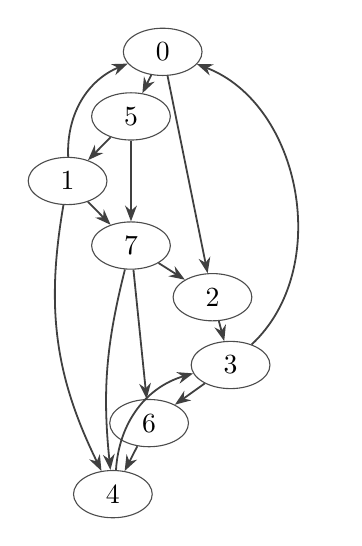
\begin{tikzpicture}[
    x=1.15cm,y=.82cm,
    v/.style={ellipse,draw=black!70,minimum width=10mm,minimum height=6mm,inner sep=0pt},
    e/.style={-{Stealth[length=2mm]},line width=.65pt,black!75}
  ]
    \node[v] (v0) at (0,7) {0};
    \node[v] (v5) at (-.35,6) {5};
    \node[v] (v1) at (-1.05,5) {1};
    \node[v] (v7) at (-.35,4) {7};
    \node[v] (v2) at (.55,3.2) {2};
    \node[v] (v3) at (.75,2.15) {3};
    \node[v] (v6) at (-.15,1.25) {6};
    \node[v] (v4) at (-.55,.15) {4};
    \draw[e] (v0)--(v5); \draw[e] (v0)--(v2);
    \draw[e] (v5)--(v1); \draw[e] (v5)--(v7);
    \draw[e] (v1)--(v7); \draw[e] (v1) to[bend left=35] (v0); \draw[e] (v1) to[bend right=18] (v4);
    \draw[e] (v7)--(v2); \draw[e] (v7)--(v6); \draw[e] (v7) to[bend right=10] (v4);
    \draw[e] (v2)--(v3);
    \draw[e] (v3)--(v6); \draw[e] (v3) to[bend right=58] (v0);
    \draw[e] (v6)--(v4); \draw[e] (v4) to[bend left=35] (v3);
  \end{tikzpicture}

  \par\smallskip
  {\small 依据原书练习 1 所附未编号有向图重绘}\par
  \end{minipage}
  \end{center}

  \begin{enumerate}[label=(\alph*),leftmargin=2.5em]
    \item 用邻接矩阵表示该图。
    \item 用 CSR 格式表示该图。每个顶点的邻居列表必须有序。
    \item 从顶点 0 开始在该图上执行并行 BFS，也就是说顶点 0 位于第 0 层。对于 BFS
    遍历的每一次迭代，分别回答：

    \begin{itemize}[leftmargin=2em]
      \item 若采用顶点中心推送式实现：
      \begin{enumerate}[label=\Alph*.,leftmargin=2.2em]
        \item 启动多少个线程？
        \item 有多少个线程会遍历自己顶点的邻居？
      \end{enumerate}

      \item 若采用顶点中心拉取式实现：
      \begin{enumerate}[label=\Alph*.,leftmargin=2.2em]
        \item 启动多少个线程？
        \item 有多少个线程会遍历自己顶点的邻居？
        \item 有多少个线程会标记自己的顶点？
      \end{enumerate}

      \item 若采用边中心实现：
      \begin{enumerate}[label=\Alph*.,leftmargin=2.2em]
        \item 启动多少个线程？
        \item 有多少个线程可能标记一个顶点？
      \end{enumerate}

      \item 若采用基于前沿的顶点中心推送式实现：
      \begin{enumerate}[label=\Alph*.,leftmargin=2.2em]
        \item 启动多少个线程？
        \item 有多少个线程会遍历自己顶点的邻居？
      \end{enumerate}
    \end{itemize}
  \end{enumerate}

  \item 实现第 \ref{sec:bfs-vertex-centric} 节所述方向优化 BFS 的主机端代码。

  \item 修改图 \ref{fig:18-17} 的内核，使每层只使用一次网格范围屏障同步，而不是三次。
\end{enumerate}

\clearpage
\begin{chapterbibliography}{9}
  \bibitem{kepner2011graph}
  J. Kepner, J. Gilbert, \emph{Graph Algorithms in the Language of Linear Algebra},
  SIAM, 2011.

  \bibitem{davis2019graphblas}
  T.A. Davis, Algorithm 1000: SuiteSparse:GraphBLAS: graph algorithms in the language
  of sparse linear algebra, \emph{ACM Transactions on Mathematical Software} 45 (4)
  (2019) 1--25.

  \bibitem{luo2010bfs}
  L. Luo, M. Wong, W.-m. Hwu, An effective GPU implementation of breadth-first search,
  in: \emph{Proceedings of the 47th Design Automation Conference}, 2010, pp. 52--55.

  \bibitem{merrill2012graph}
  D. Merrill, M. Garland, A. Grimshaw, Scalable GPU graph traversal,
  \emph{ACM SIGPLAN Notices} 47 (8) (2012) 117--128.

  \bibitem{fender2022cugraph}
  A. Fender, B. Rees, J. Eaton, RAPIDS cuGraph, in: \emph{Massive Graph Analytics},
  Chapman and Hall/CRC, 2022, pp. 483--493.
\end{chapterbibliography}


% 第 19 章暂缺；显式设置计数器，使先行完成的本章保持原书编号。
\setcounter{chapter}{19}
\chapter{大语言模型}
\label{chap:large-language-models}

\setcounter{footnote}{0}

\newcommand{\chTwentyBox}[1]{%
  \fbox{\rule{0pt}{1.65em}\makebox[7.2em][c]{\small #1}}%
}
\newcommand{\chTwentySmallBox}[1]{%
  \fbox{\rule{0pt}{1.35em}\makebox[4.8em][c]{\scriptsize #1}}%
}
\newcommand{\chTwentyCell}[1]{%
  \fbox{\rule{0pt}{1.25em}\makebox[1.7em][c]{\scriptsize $#1$}}%
}
\newcommand{\chTwentyTextCell}[1]{%
  \fbox{\rule{0pt}{1.25em}\makebox[1.7em][c]{\scriptsize #1}}%
}
\newcommand{\chTwentyNewCell}[1]{%
  \fcolorbox{black}{gray!25}{%
    \rule{0pt}{1.25em}\makebox[1.7em][c]{\scriptsize $#1$}}%
}
\newcommand{\chTwentyArrow}{\ensuremath{\longrightarrow}}

在 Google 研究人员于 2017 年提出 Transformer \cite{ch20-1} 之前，语言任务主要建立
在 IBM 开创的统计语言建模技术之上（例如 \cite{ch20-2}）。2018 年，Google 推出了
基于 Transformer 的 BERT 语言模型，并在自然语言任务中取得了前所未有的结果。此后，
Transformer 架构\footnote{本章中的“架构”指神经网络架构，而不是本书其他章节中所说的
硬件架构。}成为基于神经网络的自然语言处理（natural language processing，NLP）深度
学习方法的基础。

此后，大语言模型（large language models，LLM）受到产业界广泛关注，并迅速发展，在
文本生成、摘要、翻译和对话等多种任务中表现出接近人类的能力。与 BERT 及更早一代的
语言模型相比，这些模型的规模增长了数个数量级，以便容纳更多训练数据。“大语言模型”
这一术语正是为了把它们与早期语言模型区分开来。LLM 最初主要用于处理和生成文本信息，
但后来也出现了多模态模型：这类模型使用视觉、音频以及科学数据等不同类型的数据进行
训练，并在这些数据上工作。

LLM 的核心思想是：给定一串此前出现的 token，预测下一个 token。这里的 token 可以是
一个单词、子词或字符。在 OpenAI ChatGPT \cite{ch20-3} 这样的聊天机器人应用中，此前
的 token 序列统称为上下文（context），它由系统提示词、用户输入以及模型已经生成的
token 组成。为了生成正确、有效或有用的结果\footnote{对于文本摘要等任务，“准确率”
未必是合适的评价指标，因为不同答案可能都正确。本章使用“准确”时，采用更一般的
“正确、有效或有用”的含义。}，LLM 通常包含数十亿个参数，例如数十层、每层数亿个
参数，并且需要在规模巨大的数据集上训练。在推理阶段，更长的上下文有助于生成更准确
的响应。模型需要通过一种称为注意力（attention）的机制维护上下文，并识别大段上下文
中与下一个 token 生成最相关的部分。因此，理解注意力机制以及 Transformer 架构，对于
理解 LLM 十分重要。Transformer 是目前把注意力机制引入 LLM 的最主流方法之一
\cite{ch20-1}。

\noindent\textbf{补充说明：}虽然本章聚焦 Transformer 和注意力机制，研究界也在持续
探索具有不同优势的其他 LLM 架构，例如状态空间模型 Mamba \cite{ch20-4}、卷积模型
Hyena \cite{ch20-5} 以及混合模型。它们在某些场景下可能具有更低的内存需求。

\section{Transformer 架构}
\label{sec:ch20-transformer}

如今大多数 LLM 都采用 Transformer 架构及其注意力机制，以捕获 token 之间的依赖关系，
并判断这些 token 在生成下一个 token 时的重要程度。注意力机制类似于神经网络内部的
分类过程：它使用 softmax 函数生成概率，而序列中每个 token 获得的概率可以看作该 token
对于生成下一个 token 的相对重要性。

Transformer 最初是为机器翻译等序列转换任务提出的，因此包含两种类型的层。编码器层
对输入 token 进行上下文化（或混合），把源语言中的符号序列（例如 token）转换成连续
表示，即浮点嵌入向量序列。解码器层接收编码器输出的连续表示，并逐个生成目标语言中的
输出 token。解码器不仅接收编码器的输出，还接收自身最近生成的 token。因此，Transformer
模型是自回归（auto-regressive）模型。

Transformer 提出之后，人们把它适配到了其他任务。根据具体任务，一个 Transformer
不一定需要同时包含两类层。例如，执行分类等判别任务的模型并不需要解码器，因为它们
不会生成目标语言中的文本。另一方面，仅解码器模型（decoder-only model）能够执行文本
生成等生成式任务。LLM 就属于这一类：它根据用户查询生成文本响应，而不是执行序列到
序列的转换。生成式任务需要多次执行模型；每次执行都根据已有 token 序列，预测候选
新输出 token 的可能性。本节重点讨论仅解码器 Transformer 的架构。关于编码器--解码器
Transformer，可参考文献 \cite{ch20-1}。

\begin{figure}[htbp]
  \centering
  \small
  \begin{tabular}{c}
    \chTwentyBox{Tokenizer（分词器）}
    \quad $\downarrow$ \quad
    \chTwentyBox{Embedding（嵌入）}
    \quad $\downarrow$ \quad
    \chTwentyBox{位置编码}\\[0.5em]
    $\downarrow$\\[-0.2em]
    \fbox{\begin{minipage}{0.75\textwidth}
      \centering
      \textbf{Transformer 层（重复多次）}\\[0.3em]
      \chTwentySmallBox{多头注意力}
      \quad $\longrightarrow$ \quad
      \chTwentySmallBox{Add \& Norm}
      \quad $\longrightarrow$ \quad
      \chTwentySmallBox{前馈网络}
      \quad $\longrightarrow$ \quad
      \chTwentySmallBox{Add \& Norm}\\[0.35em]
      残差连接与层归一化贯穿各子层
    \end{minipage}}\\[0.5em]
    $\downarrow$\\[-0.2em]
    \chTwentyBox{Un-embedding（反嵌入）}
    \quad $\longrightarrow$ \quad
    \chTwentyBox{下一个 token 的概率分布}
  \end{tabular}
  \caption{仅解码器 Transformer 的基线架构（依据原书图 20.1 临时重绘，未包含
  KV cache）。}
  \label{fig:20-1}
\end{figure}

图 \ref{fig:20-1} 展示了一个基于仅解码器 Transformer 的 LLM 设计。下面简要说明
其中的主要组成部分。

\begin{enumerate}[label=\arabic*.,leftmargin=2.7em]
  \item \textbf{Tokenizer（分词器）}把输入文档或查询中的文本转换为 token 序列，即
  用来表示一个字符或一小段字符的整数 ID。文本到 token 的映射建立在这样的思想上：
  可以从目标语言的训练文档中学习出一个有限词表。分词器学习并识别出的所有不重复
  token 构成 LLM 的词表。每个分词器都有自己对 token 的定义，以及把文本输入转换成
  token 的方法。

  在训练 LLM 时，模型会为训练文档中遇到的 token 分配唯一 ID。每当分词器决定从下
  一个文本片段形成一个 token 时，它都会检查相同片段是否已经出现过。如果没有，就发现
  了一个新的文本片段，并为它分配新的 ID；这个 ID 将作为该片段在模型中的表示。文本
  片段与 token ID 的映射会被记录下来，供以后查找。如果片段此前已经出现，分词器就
  通过映射找到原先分配的 token ID。文本片段到 token ID 的映射是训练过程的结果之一。

  在推理阶段，每次分词器从文本片段形成 token 时，都会查找该片段对应的 token ID，
  并把它作为分词器的下一个输出。严格地说，token 是构成 LLM 词表的文本片段，而
  token ID 是 token 在模型内部的整数表示。除非需要特别区分，本章在描述 LLM 运算
  时会交替使用 token 和 token ID 这两个术语。

  \item \textbf{Embedding（嵌入）层}把分词器生成的 token（即 token ID）转换成嵌入
  向量，也就是 token 的浮点向量表示。这里交替使用 embedding 和 embedding vector
  这两个说法。转换通常通过查找嵌入表完成。训练过程中也会从文档中学习每个 token 的
  嵌入值。之所以要进行这种转换，是因为 LLM 是使用数值方法训练的机器学习模型。训练
  通常采用梯度下降方法，要求模型函数可微，并且输入和参数采用连续形式；浮点表示是
  对连续值的一种近似。

  \item \textbf{位置编码（positional encoding）层}把序列顺序信息加入输入 token 的
  嵌入向量。位置编码告诉注意力机制 token 在序列中的物理位置和相互距离；这些因素会
  在判断此前输入和输出 token 对下一个 token 生成的相关性时发挥作用。

  当前对话中的完整 token 序列（包括用户输入、系统添加的输入和模型输出）会按照生成
  顺序累积成一个矩阵。矩阵的每一行是一个 token 的嵌入向量，该矩阵作为第一个
  Transformer 层的输入。

  \item \textbf{Transformer 层}对嵌入进行变换，以提取 token 之间的依赖关系。每个
  Transformer 层包含一个多头注意力子层、一个加法与归一化子层、一个前馈子层，以及
  另一个加法与归一化子层。

  \item \textbf{多头注意力子层}由并行排列的多个注意力头组成。每个注意力头通过矩阵
  乘法对嵌入执行线性投影。线性投影所用矩阵是在训练过程中学习得到的，它们实际上
  对嵌入向量执行坐标变换，使后续的相似度比较更有效。投影结果再经过另一次矩阵乘法，
  测量一个 token 与此前已经生成的所有 token 之间的相似度。多个注意力头的输出会被
  拼接起来，通常再经过线性变换，形成多头注意力子层的组合输出。

  \item \textbf{加法与归一化（Add \& Norm）子层}位于多头注意力子层之后。每个前馈
  子层或注意力子层之后的加法操作都建立残差连接，以保留原始输入的信息。归一化操作
  通过把结果向量归一化到下一层所需的数值范围，稳定计算过程并改善收敛。归一化通常
  使用输入嵌入向量元素的均值 $\mu$、标准差 $\sigma$ 以及学习得到的参数 $\gamma$、
  $\beta$。

  \item \textbf{前馈子层}通常由两个线性变换和中间的 ReLU 激活组成。直观地说，注意力
  层识别 token 之间的相似性或依赖关系，并根据相似度加权组合此前 token 的嵌入向量，
  生成新的嵌入版本；前馈子层则为这些新的嵌入版本增加语义含义。关于 ReLU 和激活
  函数的定义，参见附录 B。

  \item 另一个 \textbf{加法与归一化子层}位于前馈子层之后，用来保留前馈子层输入中的
  信息、改善收敛，并最终生成该 Transformer 层的输出。
\end{enumerate}

模型中 Transformer 层的数量称为模型深度，不同 LLM 的深度差别很大。执行大规模矩阵
乘法的注意力头，是 Transformer 架构中计算开销最大的部分，也是本章后续内容的重点。
最后，\textbf{反嵌入（un-embedding）层}把最后一个 Transformer 层输出的嵌入转换成
token 上的概率分布，用于生成下一个输出 token。

模型维度对于生成高质量回答非常重要。第一维是模型深度，即 Transformer 层的数量。
更深的模型提供更多层级的分类器，因而能够捕获更一般的依赖模式。第二维是每个嵌入
向量中的元素数量，称为头维度（head dimension）。更宽的嵌入向量能够捕获更多语义
信息，区分不同概念，并发现更有意义的依赖关系。第三维是每个注意力子层中的头数量；
不同注意力头能够捕获 token 之间不同类型的依赖。模型参数量约等于这些模型维度相关
规模的乘积，实际模型可能包含数十亿甚至数万亿个参数（模型权重）。

虽然 LLM 需要较长上下文才能生成准确响应，但用户输入通常过于简短且隐含信息较多，
不能提供充分的上下文。一个常见补救方法是使用检索增强生成（retrieval-augmented
generation，RAG）：检索相关文档，把更具体、更及时的上下文信息与用户输入拼接起来，
形成更大、更丰富的上下文。

在 LLM 训练期间，最重要的计算通常是大规模矩阵--矩阵乘法。注意力头和前馈子层都会
执行这种运算，并可以使用第 15 章介绍的高级优化策略。正因为矩阵乘法占据主要计算
开销，注意力头成为 LLM 中最昂贵的计算组件。下一节将详细讨论注意力头的设计及其所
执行的矩阵乘法。

\section{多头注意力}
\label{sec:ch20-multi-head-attention}

每个注意力子层包含多个头。多个头共同执行多个分类任务，并同时捕获不同类型的依赖，
例如位置依赖（token 之间的距离）、语义依赖（同义词或主题）、上下文依赖（把冠词与
名词联系起来）和句法依赖（把动词与宾语联系起来）。这种注意力头的专门化是在训练
过程中形成的。不同头的权重矩阵采用不同初始化；反向传播的梯度下降会避免不同头
之间的功能重叠，并通过 dropout（随机置零输出或概率）和层归一化（归一化激活值）等
技术抑制过拟合。

注意力头彼此独立，因此可以很容易地分配到多个线程块上并发计算。不同头的设计相同，
所以下面只展示一个注意力头。图 \ref{fig:20-2} 给出了一个注意力头的计算过程。
输入矩阵 $X$ 的每一行对应 LLM 当前已经生成的 token 的嵌入向量，包括系统提示词、
用户输入、系统对用户输入的补充信息以及已经生成的输出 token。对于第一个 Transformer
层的注意力子层，$X$ 的每一行包含位置编码组件生成的嵌入；对于后续 Transformer 层，
输入 $X$ 就是前一层的输出。

当前已经生成的 token 数量，也就是矩阵 $X$ 的行数，称为序列长度或上下文长度，后文
统一记作 $N$。在聊天机器人应用中，随着用户与系统的对话持续进行，$N$ 会逐渐增长。
支持较大 $N$ 的模型可以利用更多上下文来消除词语和短语的歧义、判断上下文相关性，
并保持连续回答之间的一致性，因此通常能够生成更可靠的 token。注意力子层通常遵循
因果策略：当前 token 的生成只能依赖此前生成的 token，而忽略未来 token。

每个嵌入向量中的元素数量，即头维度，记作 $d$。因此，$X$ 是一个 $N\times d$ 矩阵。
头维度和每个子层中的头数量通常被称为 LLM 的隐藏维度，它们是模型的内部设计参数，
通常不会直接暴露给 LLM 用户。

\begin{figure}[htbp]
  \centering
  \small
  \begin{tabular}{c@{\quad}c@{\quad}c@{\quad}c}
    $X_{N\times d}$ & $\xrightarrow{\;W_Q\;}$ & $Q_{N\times d}$ &
    $\xrightarrow{\quad}$\\[0.35em]
    \rotatebox{90}{$\begin{matrix}\xrightarrow{\;W_K\;}\\[-0.2em]
    \xrightarrow{\;W_V\;}\end{matrix}$} & &
    $\begin{matrix}K_{N\times d}\\ V_{N\times d}\end{matrix}$ &\\[0.5em]
    \multicolumn{4}{c}{$S=QK^{\mathsf T}\ (N\times N)
      \quad\xrightarrow{\;+\ M\;}\quad
      P=\operatorname{softmax}(S+M)\ (N\times N)
      \quad\xrightarrow{\;\times V\;}\quad
      O_{N\times d}$}
  \end{tabular}
  \caption{一个注意力头计算中涉及的矩阵（依据原书图 20.2 临时重绘）。
  为简化图示，省略了作用于 $S=QK^{\mathsf T}$ 的缩放因子 $1/\sqrt d$。}
  \label{fig:20-2}
\end{figure}

注意力子层的第一步是计算三个矩阵：query（查询，$Q$）、key（键，$K$）和 value
（值，$V$）。如图 \ref{fig:20-2} 左侧所示，这些矩阵由 $X$ 的行向量经过线性投影
或坐标变换得到，即把输入矩阵分别乘以三个权重矩阵 $W_Q$、$W_K$ 和 $W_V$。在本章
的简化讨论中，这三个坐标变换矩阵都是 $d\times d$ 矩阵，并由训练过程得到。$Q$、
$K$ 和 $V$ 的每一行中的元素，都是 $X$ 同一行中 $d$ 个元素的线性组合；三种变换的
差异由 $W_Q$、$W_K$ 和 $W_V$ 中的权重值决定。

\noindent\textbf{译者注：}为简化说明，本章假设三个权重矩阵是方阵。一般情况下，
$W_Q$、$W_K$ 和 $W_V$ 的尺寸分别可以是 $d_x\times d_q$、$d_x\times d_k$ 和
$d_x\times d_v$；由于需要计算 $QK^{\mathsf T}$，必须有 $d_q=d_k$。

注意力子层的第二步由下面的公式给出，也对应图 \ref{fig:20-2} 的右侧：
\begin{equation}
  O =
  \operatorname{softmax}\!\left(
    \frac{QK^{\mathsf T}}{\sqrt{d}} + M
  \right)V .
\label{eq:ch20-attention}
\end{equation}

由于 $Q$ 是 $N\times d$ 矩阵，$K^{\mathsf T}$ 是 $d\times N$ 矩阵，矩阵乘法
$QK^{\mathsf T}$ 会生成一个 $N\times N$ 矩阵，记作图 \ref{fig:20-2} 中的 $S$。
$QK^{\mathsf T}$ 的元素 $(i,j)$ 是 token $i$ 的线性投影嵌入向量（$Q$ 的第 $i$ 行）
与 token $j$ 的线性投影嵌入向量（$K^{\mathsf T}$ 的第 $j$ 列，也就是 $K$ 的第 $j$
行）之间的内积。如果两个输入向量都已归一化，内积可以看作它们的余弦相似度。两个
向量越相似，它们之间的夹角越小，余弦相似度也越大。因此，$N\times N$ 的乘积矩阵
可以看作嵌入向量之间的相似度地图。

缩放因子 $1/\sqrt d$ 作用于 $S=QK^{\mathsf T}$ 的所有元素，用于防止头维度较大时
矩阵乘法的点积过度增长。过大的 $S$ 元素会使 softmax 饱和，并在基于梯度下降的训练
中产生很小、甚至消失的梯度 \cite{ch20-1}。图 \ref{fig:20-2} 及相关讨论为简洁起见
省略了缩放因子；稍后可以看到，把它并入 CUDA softmax 实现非常直接。

掩码矩阵 $M$ 会把 $QK^{\mathsf T}/\sqrt d$ 中所有列索引大于行索引的元素加上
$-\infty$。这样便实现了因果策略：生成某个 token 时，不能受到该 token 之后才生成
的 token 的影响。

softmax 函数把 $QK^{\mathsf T}+M$ 的每一行转换为概率分布。设该矩阵第 $r$ 行、第
$c$ 列的元素为 logit $l_{r,c}$，softmax 生成的概率为 $p_{r,c}$。为了避免指数函数
溢出，令 $m_r$ 为该行的最大元素，并采用数值稳定的形式：
\begin{equation}
  p_{r,c}
  =
  \frac{e^{l_{r,c}}}{\sum_{j=1}^{N} e^{l_{r,j}}}
  =
  \frac{e^{l_{r,c}-m_r}}
       {\sum_{j=1}^{N}e^{l_{r,j}-m_r}},
  \qquad
  m_r=\max_{1\leq j\leq N} l_{r,j}.
\label{eq:ch20-softmax}
\end{equation}

直接计算 $e^{l_{r,c}}$ 可能溢出，因此在取指数之前先从 $l_{r,c}$ 中减去
$m_r=\max_{1\leq j\leq N}(l_{r,j})$。这个操作保持了数值稳定性，同时不改变结果：
从 $l_{r,c}$ 中减去 $m_r$ 等价于把分子和分母都乘以 $e^{-m_r}$。

由于因果掩码，行索引 $r$ 小于列索引 $c$ 的 logit 会变成 $-\infty$，于是
$e^{l_{r,c}-m_r}=0$。因此，矩阵
$P=\operatorname{softmax}(QK^{\mathsf T}+M)$ 的每一行，都是 token $r$ 的嵌入与
此前生成 token 的嵌入之间相似度所决定的概率分布。softmax 输出矩阵是一个下三角
矩阵：当 $r<c$ 时，元素 $p_{r,c}$ 为零。

注意力子层的最后一步是计算 $N\times N$ 的概率矩阵 $P$ 与 $V$ 的矩阵乘法。对于
每个 token，这个矩阵乘法都会生成一个新的嵌入向量；新向量的每个元素，都是 $V$
矩阵中同一列元素的相似度/概率加权和。换句话说，输出矩阵 $O$ 中每个 token 的新
嵌入，是此前生成 token 的嵌入向量的相似度加权和。之后，$O$ 会经过加法与归一化、
前馈等子层，成为下一个注意力子层的输入矩阵 $X$。

\begin{figure}[htbp]
  \centering
  \small
  \begin{tabular}{c@{\qquad}c}
    \fbox{\begin{minipage}{0.39\textwidth}
      \centering
      \textbf{摘要/预填充阶段}\\[0.3em]
      系统提示词 + 用户输入 + RAG 文档\\
      $\downarrow$ tokenizer / embedding\\
      $X$：一整个 token 序列\\
      $\downarrow$\\
      一次 Transformer 前向传播\\
      $\downarrow$\\
      第一个输出 token
    \end{minipage}}
    &
    \fbox{\begin{minipage}{0.39\textwidth}
      \centering
      \textbf{生成/解码阶段}\\[0.3em]
      把新 token 追加到上下文\\
      $\downarrow$\\
      每次处理一个新 token\\
      $\downarrow$\\
      生成下一个 token\\
      $\circlearrowleft$ 直到 EOS
    \end{minipage}}
  \end{tabular}
  \caption{LLM 推理的摘要（prefill）阶段和生成（decode）阶段
  （依据原书图 20.3 临时重绘）。}
  \label{fig:20-3}
\end{figure}

基于图 \ref{fig:20-1} 的仅解码器架构进行 LLM 推理时，首先进入摘要阶段：系统提示词、
用户输入以及系统补充的 token（例如 RAG 检索结果）拼接起来，形成第一个 Transformer
层的输入矩阵 $X$。摘要阶段中，每个注意力头涉及的矩阵和计算如图 \ref{fig:20-2}
所示。累积的 $X$ 依次经过各个 Transformer 层；每层生成下一层的输入。最后一层完成
后，反嵌入层生成一个文本片段形式的输出 token。下一次推理迭代进入自回归阶段，也称
解码阶段或生成阶段。新生成的文本片段被送回分词器，其嵌入向量作为 $X$ 的新行追加
到第一个 Transformer 层，然后再次激活各层以生成下一个文本片段。

图 \ref{fig:20-3} 用一个玩具例子说明两个阶段。摘要阶段首先把系统提示和用户提示
组成的初始序列送入分词器和嵌入层，并累积到矩阵 $X$ 中。为简化起见，例子省略系统
提示词和用户输入中通常存在的前导语。用户输入为 “The title of this book is
Programming”，希望 LLM 补全本书标题。

假设这个例子使用完整单词作为 token。摘要阶段中，分词器、嵌入层和位置编码层把用户
输入产生的七个 token 的嵌入向量累积到第一个 Transformer 层的 $X$ 矩阵中。LLM
随后调用第一个 Transformer 层；该层完成后激活第二层，以此类推。每层被激活时都会
计算自己的 $K$、$V$、$Q$、$QK^{\mathsf T}$ 和 $O$，然后激活下一层。所有 Transformer
层和最后的反嵌入层完成后，LLM 生成第一个输出 token “Massively”。

生成第一个输出 token 后，LLM 进入生成阶段。每个输出 token 都根据初始提示以及此前
所有迭代生成的输出 token 产生。在例子中，摘要阶段末尾生成的 “Massively” 会成为
生成阶段第一次迭代的输入，并由这次迭代产生下一个输出 token。对于每个新输出 token，
LLM 都会生成一个对应的新嵌入向量，也就是矩阵 $X$ 的新行，并让它经过各个 Transformer
层。第一次生成迭代得到 “Parallel”，它会成为下一次迭代的输入。生成阶段会持续进行，
直到产生 end-of-sequence（EOS）token。

\section{在 CUDA 中实现注意力}
\label{sec:ch20-cuda-attention}

图 \ref{fig:20-1} 所示 Transformer 架构中的注意力计算包含两次矩阵乘法、一次矩阵
逐元素缩放、一次矩阵加法和 softmax 计算。矩阵乘法可以使用自定义 CUDA 矩阵乘法
内核，也可以调用 cuBLAS 等库中高度优化的 GEMM 函数。缩放因子 $1/\sqrt d$ 可以
在自定义内核执行 $QK^{\mathsf T}$ 时应用，也可以作为 cuBLAS GEMM API 的缩放参数
$\alpha$。注意力计算中唯一的新部分是 softmax 的实现，因此本节重点讨论 CUDA
softmax，并把其余部分留作练习。

图 \ref{fig:20-4} 展示了一个把与 $M$ 的矩阵加法和 softmax 计算融合在同一内核中的
CUDA 实现。融合内核避免在 softmax 之前额外遍历输入矩阵 $S$，从而提高算术强度和
GPU 利用率。

\begin{figure}[htbp]
  \centering
  \begin{lstlisting}[language=C++,basicstyle=\ttfamily\tiny]
// Figure 20.4: causal softmax kernel
#define BLOCK_SIZE 256
#define NEG_INFINITY (-INFINITY)

__global__ void softmax_kernel(float* S, float* D, float* P, int N)
{
    typedef cub::BlockReduce<float, BLOCK_SIZE> BlockReduce;
    __shared__ typename BlockReduce::TempStorage temp_store;
    __shared__ float max_or_sum;

    float* S_row = &S[blockIdx.x * N];
    float max_val_thread = NEG_INFINITY;

    for (int idx = threadIdx.x;
         idx <= blockIdx.x;
         idx += blockDim.x) {
        if (S_row[idx] > max_val_thread)
            max_val_thread = S_row[idx];
    }

    __syncthreads();
    float max_val_row =
        BlockReduce(temp_store).Reduce(max_val_thread, cub::Max());

    if (threadIdx.x == 0)
        max_or_sum = max_val_row;
    __syncthreads();
    max_val_row = max_or_sum;

    float sum_thread = 0.f;
    for (int idx = threadIdx.x;
         idx <= blockIdx.x;
         idx += blockDim.x) {
        sum_thread += exp(S_row[idx] - max_val_row);
    }

    __syncthreads();
    float sum_row =
        BlockReduce(temp_store).Reduce(sum_thread, cub::Sum());

    if (threadIdx.x == 0)
        max_or_sum = sum_row;
    __syncthreads();
    sum_row = max_or_sum;

    for (int idx = threadIdx.x;
         idx < N;
         idx += blockDim.x) {
        P[blockIdx.x * N + idx] =
            idx <= blockIdx.x
                ? exp(S_row[idx] - max_val_row) / sum_row
                : 0.f;
    }

    if (threadIdx.x == 0)
        D[blockIdx.x] = sum_row;
}
  \end{lstlisting}
  \caption{融合因果掩码和 softmax 的 CUDA 内核（依据原书图 20.4 整理）。
  代码标识符保持原文；本图为可复制版本。}
  \label{fig:20-4}
\end{figure}

该内核的执行配置是一个一维线程块网格。内核假定线程块数量
\code{gridDim.x} 等于矩阵 $S$ 的行数，也就是序列长度 $N$。底本把未使用的
\code{gridDim.y} 和 \code{gridDim.z} 描述为 0；在合法的 CUDA 启动配置中，未使用
维度通常取 1，本译稿把这句话理解为“只使用 x 维”，而不把 0 当作可直接传入的网格
维度。这个假设把上下文长度限制在 x 维允许的最大线程块数以内。若需要更长上下文，
可以在内核中增加外层循环，让网格中的线程块迭代处理 $S$ 的所有行。

每个线程块是一维块，包含 \code{BLOCK_SIZE} 个线程。由于一个线程块协同处理 $S$
的一行，应选择合适的 \code{BLOCK_SIZE}：既要减少线程块处理该行所需的迭代次数，
也要尽量提高 GPU 上 SM 的占用率。

当缩放因子已经在 $QK^{\mathsf T}$ 矩阵乘法中应用，并且因果策略已经融合到 softmax
中时，一行 $S$ 的每个元素都可以看作公式 \eqref{eq:ch20-softmax} 中的
$l_{r,c}$。代码前半部分先找出分配给线程块的那一行的最大元素，即公式中的 $m_r$。
每个线程检查自己负责的一段元素，并把局部最大值保存在私有变量
\code{max_val_thread} 中。循环条件 \code{idx <= blockIdx.x} 很关键：它忽略行索引
\code{blockIdx.x} 小于列索引 \code{idx} 的元素，从而不显式构造掩码矩阵 $M$ 就实现
因果策略。

线程退出循环后，每个线程只持有自己检查部分的最大值。块内同步确保所有线程都完成
检查，然后调用 CUB 的 \code{BlockReduce} 求整行最大值。归约结果由
\code{threadIdx.x == 0} 的线程获得；该线程把结果写入共享内存变量
\code{max_or_sum}，再通过块内同步把结果广播给所有线程。代码的这部分本质上是带
线程粗化的归约。

接下来，代码以相同的方式求公式 \eqref{eq:ch20-softmax} 的分母。线程首先计算私有
部分和；循环条件继续实现因果策略。同步后，CUB 的 \code{BlockReduce} 求出整行的
指数和，线程 0 再通过共享内存广播最终结果。最后一个循环遍历行中的全部元素，把
因果掩码区域写成 0，把其余元素写入输出矩阵 $P$。分母同时写入输出向量 $D$，以便
训练阶段复用。

总之，该 softmax 内核在一个内核调用中同时实现因果策略和 softmax，只使用块级
\code{__syncthreads()}，不需要额外的全局屏障。读者可以在此基础上补充生成 $S$
和 $O$ 的矩阵乘法，完成整个注意力子层。

\section{KV 缓存}
\label{sec:ch20-kv-cache}

如果按照图 \ref{fig:20-3} 的直接方式实现，图 \ref{fig:20-1} 的 Transformer 架构
存在明显低效之处。在生成阶段的每次迭代中，每个 Transformer 层都要执行五次矩阵
乘法。由于序列长度 $N$ 可能增长到数万个 token 甚至更多，这些矩阵乘法的开销会非常
大。但从一次解码迭代到下一次迭代，输入矩阵 $X$ 只增加一行，因此有必要问：每次
迭代真的都需要执行完整的矩阵乘法吗？答案是否定的。

\begin{figure}[htbp]
  \centering
  \small
  \resizebox{0.98\textwidth}{!}{%
  \begin{tabular}{c@{\qquad}c@{\qquad}c}
    \begin{tabular}{c}
      $X_N$\\[-0.2em]
      \chTwentyCell{x_0}\\
      \chTwentyCell{x_1}\\
      \vdots\\
      \chTwentyNewCell{x_N}
    \end{tabular}
    &
    $\xrightarrow{\;W_Q,W_K,W_V\;}$
    &
    \begin{tabular}{c}
      $Q_N,\ K_N,\ V_N$\\[-0.2em]
      前 $N$ 行保持不变\\
      新增最后一行
    \end{tabular}\\[1em]
    \multicolumn{3}{c}{
      \begin{tabular}{c}
        $QK^{\mathsf T}$ 从 $N\times N$ 变为 $(N+1)\times(N+1)$\\[-0.1em]
        \chTwentyTextCell{旧} \chTwentyTextCell{旧} \chTwentyTextCell{新}\\
        \chTwentyTextCell{旧} \chTwentyTextCell{旧} \chTwentyTextCell{新}\\
        \chTwentyTextCell{新} \chTwentyTextCell{新} \chTwentyTextCell{新}
      \end{tabular}
    }
  \end{tabular}
  }%
  \caption{从一次 LLM 迭代到下一次迭代时减少矩阵乘法工作的机会
  （依据原书图 20.5 临时重绘；灰色表示新增或需要处理的部分）。}
  \label{fig:20-5}
\end{figure}

图 \ref{fig:20-5} 突出了从迭代 $i$（$N=i$）到迭代 $i+1$（$N=i+1$）时各矩阵
新增的部分。输入矩阵 $X$ 在底部增加一个新行，即新 token 的嵌入向量，因此尺寸从
$N\times d$ 变成 $(N+1)\times d$。$Q$、$K$ 和 $V$ 的情况类似：它们都变成
$(N+1)\times d$ 矩阵，而新增的底部行分别由 $X$ 的新底行与 $W_Q$、$W_K$、$W_V$
执行向量--矩阵乘法得到。

生成 $QK^{\mathsf T}$ 稍微复杂一些。新矩阵的尺寸是 $(N+1)\times(N+1)$，但除第
$(N+1)$ 行和第 $(N+1)$ 列外，其余内容基本与上一次迭代相同。例如，乘积矩阵的
元素 $(0,0)$ 由 $Q$ 的第 0 行与 $K$ 的第 0 行（即 $K^{\mathsf T}$ 的第 0 列）
的内积生成，而这两行在两次迭代中都没有变化。因此该元素也不变。一般而言，只要
$r$ 和 $c$ 都小于 $N$，$QK^{\mathsf T}$ 的元素 $(r,c)$ 就由两次迭代中均未变化
的 $Q$、$K$ 行生成，因而保持不变。

新 $N$ 行的 $QK^{\mathsf T}$ 可以通过新 $Q$ 行与完整 $K^{\mathsf T}$ 的向量--矩阵
乘法计算。新 $N$ 列中的元素由于因果策略的零掩码都为零，因为此前生成的 token 不
应该受到后来生成 token 的影响；唯一例外是新行新列交叉处的元素，它属于新行计算
的一部分。

softmax 的输出也可以从上一次迭代增量更新。softmax 作用于 $QK^{\mathsf T}$ 的
每一行；除了新行之外，每一行新增的第 $N$ 个元素都是 0，因此不会稀释原有元素的
概率，也不会改变这些行的 softmax 结果。读者可以验证：在迭代 $N+1$ 中，$O$ 的
前 $N$ 行仍然与上一次迭代相同，只需用新一行 softmax 输出与新 $V$ 做向量--矩阵
乘法即可得到新行。

\begin{figure}[htbp]
  \centering
  \small
  \begin{tabular}{c@{\quad}c@{\quad}c}
    \begin{tabular}{c}
      新输入行\\
      $X'$\\[0.3em]
      $\downarrow$\\
      $Q'$、$K'$、$V'$
    \end{tabular}
    &
    $\longrightarrow$
    &
    \begin{tabular}{c}
      KV cache 中的旧 $K,V$\\
      $\left[\begin{array}{c}K\\V\end{array}\right]
      \quad+\quad
      \left[\begin{array}{c}K'\\V'\end{array}\right]$\\[0.4em]
      $\begin{gathered}
        \downarrow\\[-0.1em]
        S'=Q'[K;K']^{\mathsf T}\\
        P'=\operatorname{softmax}(S'+M)\\
        O'=P'[V;V']
      \end{gathered}$
    \end{tabular}
  \end{tabular}
  \caption{使用 KV cache 的生成阶段涉及的向量和矩阵
  （依据原书图 20.6 临时重绘）。}
  \label{fig:20-6}
\end{figure}

图 \ref{fig:20-6} 展示了生成 $Q$、$K$、$V$ 和 $O$ 新部分时涉及的向量和矩阵。每次
迭代，多头注意力子层只需要接收 $X$ 的一个新行，因此只需向下一层传递 $O$ 的一个
新行。不过，生成阶段的注意力计算仍然需要完整的 $K$ 和 $V$。一种常见优化是把
$K$ 和 $V$ 记忆化，也就是保存起来供以后复用，这便形成了 KV cache。
\footnote{这里的 KV 与键值存储（key-value store）文献中的术语不应混淆，但二者
具有类比关系：LLM 推理输出的是 $V$ 的加权和，权重与 query 和 key 的接近程度
相关。}

\begin{figure}[htbp]
  \centering
  \small
  \begin{tabular}{c}
    \fbox{\begin{minipage}{0.82\textwidth}
      \centering
      \textbf{Prefill（摘要）}\\
      初始 token 序列 $\longrightarrow$ 各 Transformer 层\\
      $K,V$ 矩阵 $\longrightarrow$ 每层自己的 KV cache
    \end{minipage}}\\[0.7em]
    $\Downarrow$\\[-0.2em]
    \fbox{\begin{minipage}{0.82\textwidth}
      \centering
      \textbf{Decode/Generation（生成）}\\
      新 token 的嵌入 $\longrightarrow$ 新 $Q',K',V'$\\
      $K',V'$ 追加到 cache $\longrightarrow$ 计算 $O'$ $\longrightarrow$ 下一个 token
    \end{minipage}}
  \end{tabular}
  \caption{使用 KV cache 的 LLM 摘要与生成阶段
  （依据原书图 20.7 临时重绘）。}
  \label{fig:20-7}
\end{figure}

图 \ref{fig:20-7} 在图 \ref{fig:20-3} 的基础上，展示了带 KV cache 的两阶段推理。
为了避免每次迭代重复计算，每个 Transformer 层生成的 $K$、$V$ 都会写入该层的
KV cache，供以后生成 token 时复用。

在摘要阶段，所有 Transformer 层生成初始的 $K$、$V$ 矩阵并填充自己的 KV cache。
因此，带 KV cache 的摘要阶段也称为预填充（prefill）阶段：各层在这一阶段把初始
$K$、$V$ 写入 cache。随后进入生成阶段，每个输出 token 都基于最后一个输出 token
以及此前所有迭代中的 $K$、$V$ 矩阵生成。最近生成的文本片段先产生一个新的嵌入
向量，并送入第一个 Transformer 层。每层先执行三个向量--矩阵乘法，分别生成 $Q$、
$K$、$V$ 的一行，即图 \ref{fig:20-6} 中的 $Q'$、$K'$、$V'$。LLM 把新行追加到
KV cache 中原有的 $K$、$V$，形成当前迭代的完整 $K$、$V$，再计算 $O'$，并把它
送入该层的后续子层，生成下一层的新输入向量。

预填充阶段仍然需要对大量 token 执行一次 Transformer 传递，并调用多次大规模矩阵--
矩阵乘法（GEMM）。它通常受计算能力限制，算术强度较高，能够较充分地利用 GPU。
下一节介绍的 FlashAttention 可以通过减少矩阵乘法与 softmax 之间中间结果的全局
内存流量，进一步加速预填充阶段。

相比之下，生成阶段每生成一个输出 token 就要执行一次 Transformer 传递。使用 KV
cache 后，每次传递主要执行向量--矩阵乘法（GEMV），通常受内存带宽限制，算术强度
较低，因而容易使 GPU 的计算资源利用不足。第 20.6 节将介绍 batching 和 speculative
decoding 等提高生成阶段算术强度的优化方法。

\section{FlashAttention}
\label{sec:ch20-flash-attention}

如果像图 \ref{fig:20-4} 那样使用独立的 softmax 内核，那么每个内核边界都会产生
全局屏障，并且整个矩阵需要多次从全局内存加载或写回。全局屏障和全局内存访问会
成为重要的性能瓶颈；FlashAttention 公式化方法 \cite{ch20-6} 可以缓解这一问题。

FlashAttention 对注意力头进行数学上的重新表达，使每个注意力头中的运算可以重新
排序并融合到一个内核中，同时以分块方式组织。在融合内核中，如图 \ref{fig:20-8}
所示，每个线程块取出 $Q$ 的一个水平面板（连续的若干行）、完整的 $K^{\mathsf T}$
和完整的 $V$，计算它们对 $O$ 的一个水平面板的贡献。图中用阴影表示属于某个线程
块的输入和输出。

\begin{figure}[htbp]
  \centering
  \small
  \resizebox{0.98\textwidth}{!}{%
  \begin{tabular}{c@{\qquad}c@{\qquad}c}
    \begin{tabular}{c}
      $Q\ (N\times d)$\\
      \fbox{\begin{tabular}{cccc}
        \chTwentyNewCell{q}&\chTwentyNewCell{q}&\chTwentyNewCell{q}&\chTwentyNewCell{q}\\
        \chTwentyNewCell{q}&\chTwentyNewCell{q}&\chTwentyNewCell{q}&\chTwentyNewCell{q}\\
        \chTwentyCell{q}&\chTwentyCell{q}&\chTwentyCell{q}&\chTwentyCell{q}
      \end{tabular}}\\[-0.2em]
      $Q_i:\ B_r\times d$
    \end{tabular}
    &
    \begin{tabular}{c}
      $K^{\mathsf T}\ (d\times N)$\\
      \fbox{\begin{tabular}{cccc}
        \chTwentyNewCell{k}&\chTwentyCell{k}&\chTwentyCell{k}&\chTwentyCell{k}\\
        \chTwentyNewCell{k}&\chTwentyCell{k}&\chTwentyCell{k}&\chTwentyCell{k}\\
        \chTwentyNewCell{k}&\chTwentyCell{k}&\chTwentyCell{k}&\chTwentyCell{k}
      \end{tabular}}\\[-0.2em]
      $K^{\mathsf T}_j:\ d\times B_c$
    \end{tabular}
    &
    \begin{tabular}{c}
      $V\ (N\times d)$\\
      \fbox{\begin{tabular}{cccc}
        \chTwentyNewCell{v}&\chTwentyNewCell{v}&\chTwentyNewCell{v}&\chTwentyNewCell{v}\\
        \chTwentyCell{v}&\chTwentyCell{v}&\chTwentyCell{v}&\chTwentyCell{v}\\
        \chTwentyCell{v}&\chTwentyCell{v}&\chTwentyCell{v}&\chTwentyCell{v}
      \end{tabular}}\\[-0.2em]
      $V_j:\ B_c\times d$
    \end{tabular}\\[1em]
    \multicolumn{3}{c}{
      $\displaystyle
      Q_iK^{\mathsf T}_j\longrightarrow S_i
      \xrightarrow{\ \operatorname{softmax}\ }P_i
      \longrightarrow P_iV_j\longrightarrow O_i$}\\[0.8em]
    \multicolumn{3}{c}{
      \fbox{\begin{tabular}{c}
        $Q_i,\ O_i$：寄存器分块\qquad
        $K^{\mathsf T}_j,\ S_i/P_i,\ V_j$：共享内存分块\\
        每次只处理 $B_c$ 列/行，并在线合并 softmax 状态
      \end{tabular}}}
  \end{tabular}
  }%
  \caption{FlashAttention 的分块方式。共享内存中的同一个 $S_i$ tile 先保存
  $S$，再原地复用为 $P$（依据原书图 20.8 临时重绘）。}
  \label{fig:20-8}
\end{figure}

此外，FlashAttention 允许线程块以分块方式遍历 $K^{\mathsf T}$ 和 $V$，同时计算
它们对 $O$ tile 的贡献。这些 tile 足够小，可以放入片上内存。每次迭代，线程块加载
$K^{\mathsf T}$ 的一个垂直面板（连续列）和 $V$ 的一个水平面板（连续行），计算它们
对 $O$ tile 的贡献。所有线程块可以并发执行，不需要全局屏障。这样，中间矩阵只以
tile 的形式保留在片上内存中，不必把它们写入全局内存，从而消除了中间矩阵对应的
全局内存流量。

FlashAttention 是对 Transformer 注意力机制的精确重构，与原始公式在数学上完全等价，
而不是近似算法。它既适用于训练（前向和反向传播），也适用于推理（前向传播）。本节
只讨论前向传播。反向传播在概念上更简单，因为不需要 softmax 重缩放，但它需要五次
矩阵乘法，而前向传播只需要两次；关于反向传播的细节，可参考原始 FlashAttention
论文 \cite{ch20-6}。

FlashAttention 的关键是分块。然而，注意力头中的分块不像矩阵乘法中的分块那样直接，
因为公式 \eqref{eq:ch20-softmax} 要求对输入的每一行执行多次扫描。softmax 计算依赖
于 $QK^{\mathsf T}+M$ 第 $r$ 行的最大值 $m_r$，以及生成概率时作为分母使用的
\[
  D_r=\sum_{j=1}^{N}e^{l_{r,j}-m_r}.
\]
按照这个形式，至少需要先扫描一行以同时收集最大值和分母，再进行另一次扫描来计算
输出矩阵 $P$ 的元素。为了保证整个 $QK^{\mathsf T}+M$ 矩阵已经准备好，softmax
内核之前还需要全局同步。

在 CUDA 中，可以通过结束一个内核并启动另一个内核实现全局屏障；也可以启动持久化
网格，使用 cooperative groups 的网格级同步 API，从而避免内核调用开销。不过，适合
矩阵乘法的线程网格配置通常不同于适合 softmax 的配置，这也是基线 CUDA 实现采用
不同内核、分别配置矩阵乘法和 softmax 的重要原因。无论选择哪种全局同步策略，多次
扫描 $S$ 的整行都会引入大量全局内存流量，显著限制吞吐量。

幸运的是，可以为分母定义部分级数，消除 softmax 对整行执行多次扫描的需要。令
$A$ 为第 $r$ 行中列位置的一个子集，定义：
\begin{equation}
  D_{r,A}=\sum_{j\in A}e^{l_{r,j}-m_{r,A}},
\label{eq:ch20-partial-denominator}
\end{equation}
其中 $m_{r,A}$ 是子集 $A$ 中元素的最大值。当 $A$ 覆盖该行的所有列位置时，
$D_{r,A}$ 就等于 $D_r$。

如果能够推导出一个组合规则，把 $A$ 的部分级数与另一个列子集 $B$ 的部分级数
合并成 $A\cup B$ 的部分级数，就可以独立地（甚至并行地）计算各个子集，然后在
结果准备好时逐步合并它们 \cite{ch20-7}。当合并后的子集覆盖第 $r$ 行的所有列时，
就能得到正确的 $D_r$。把 $D_{r,A}$ 与 $D_{r,B}$ 合并的规则为：
\begin{equation}
\begin{aligned}
  D_{r,A\cup B}
  &=\sum_{j\in A\cup B}e^{l_{r,j}-m_{r,A\cup B}}\\
  &=D_{r,A}e^{m_{r,A}-m_{r,A\cup B}}
    +D_{r,B}e^{m_{r,B}-m_{r,A\cup B}},
\end{aligned}
\label{eq:ch20-denominator-composition}
\end{equation}
其中 $m_{r,A\cup B}$ 是 $m_{r,A}$ 和 $m_{r,B}$ 中较大的一个。上式的拆分要求
$A$ 和 $B$ 不包含重复元素。在下面的 CUDA 实现中，$A$ 和 $B$ 是 $S$ 每一行的
不同 tile，因此这个条件天然满足。只要同时保存每个子集对应的最大值，就可以使用
这个规则合并两个部分和。

FlashAttention 进一步把同样的组合规则应用到输出矩阵 $O$。先考虑 $O$ 的一个元素
$o_{r,c}$，它是 $P$ 的第 $r$ 行与 $V$ 的第 $c$ 列之间的内积。只考虑行 $r$ 的
子集 $A$ 时，定义部分输出：
\begin{equation}
  o_{r,c,A}
  =\sum_{j\in A}p_{r,j,A}v_{j,c}
  =\frac{1}{D_{r,A}}
    \sum_{j\in A}e^{l_{r,j}-m_{r,A}}v_{j,c}.
\label{eq:ch20-partial-output}
\end{equation}
$p_{r,j,A}$ 是只考虑子集 $A$ 时的中间概率值，$m_{r,A}$ 也只取子集 $A$ 中
元素的最大值，而不是整行的最大值。随着更多元素并入 $A$，当 $A$ 最终覆盖整行时，
$p_{r,j,A}$ 就会变成完整 softmax 中的 $p_{r,j}$。

根据分母的组合规则，部分输出的组合规则为：
\begin{equation}
\begin{aligned}
  o_{r,c,A\cup B}
  &=
  \frac{D_{r,A}e^{m_{r,A}-m_{r,A\cup B}}}
       {D_{r,A\cup B}}\,o_{r,c,A}\\
  &\quad+
  \frac{D_{r,B}e^{m_{r,B}-m_{r,A\cup B}}}
       {D_{r,A\cup B}}\,o_{r,c,B}.
\end{aligned}
\label{eq:ch20-output-composition}
\end{equation}

也就是说，在把两个子集的部分输出合并为完整输出前，必须根据各自的最大值和分母
对它们进行重缩放。这个规则对于行的任意子集都成立，但当子集是由 $Q$ 和
$K^{\mathsf T}$ 的 tile 生成的连续片段时尤其有用。图 \ref{fig:20-8} 正是利用
这一规则实现 FlashAttention 的分块方法 \cite{ch20-8}。

\begin{figure}[htbp]
  \centering
  \begin{lstlisting}[language=C++,basicstyle=\ttfamily\tiny]
#define WARP_SIZE 32
#define BLOCK_SIZE 512
#define N_WARPS (BLOCK_SIZE / WARP_SIZE)
#define B_r 32
#define B_r_warp (B_r / N_WARPS)
#define B_c 32
#define d 128

__global__ void flashattention_forward_kernel(
    const float* Q,
    const float* K,
    const float* V,
    const int N,
    const float scaling,
    float* out_D,
    float* out_O)
{
    const int T_r = N / B_r;
    const int T_c = N / B_c;
    const int d_size = d > WARP_SIZE ? d / WARP_SIZE : 1;

    __shared__
    float KT_j[B_c * d + ((B_c * d) >> LOG_NUM_BANKS)];
    __shared__ float S_i[B_r][B_c];
    __shared__ float V_j[B_c][d];

    for (int i = blockIdx.x; i < T_r; i += gridDim.x) {
        float O_i[B_r_warp][d_size];
        float D_i[B_r_warp];
        float m_i[B_r_warp];

        initialize(O_i, D_i, m_i);

        float Q_i[B_r_warp][d_size];
        load_Q(Q, Q_i, i);

        for (int j = 0; j < T_c; j++) {
            load_KT_and_V(K, V, KT_j, V_j, j);
            __syncthreads();

            for (int ii = 0; ii < B_r_warp; ii++) {
                float curr_max_warp =
                    compute_S_and_max(
                        Q_i, KT_j, S_i, i, j, ii, scaling);

                float last_m =
                    update_m_and_D(
                        m_i, D_i, curr_max_warp, ii);

                float curr_sum_warp =
                    compute_P_and_update_D(
                        S_i, m_i, D_i, i, j, ii);

                compute_O(
                    S_i, V_j, O_i, ii, last_m, m_i);
            }
        }

        __syncthreads();
        store_O(out_O, out_D, O_i, D_i, i, N);
    }
}
  \end{lstlisting}
  \caption{FlashAttention 前向传播的 CUDA 内核主体（依据原书图 20.9 整理）。
  该示例处理一个注意力头；多头版本可以增加网格维度。}
  \label{fig:20-9}
\end{figure}

图 \ref{fig:20-9} 的内核计算一个注意力头的前向传播。完整网格参与该计算；在更
完整的实现中，可以通过增加线程块网格的其他维度，在同一个内核中计算多个头。相同
的分块方式也适用于 LLM 推理的预填充阶段。图中示例使用 32 位浮点数，而当前高性能
实现通常使用 16 位甚至 8 位浮点数，并利用 GPU Tensor Core 的吞吐能力。

该内核假定输入矩阵 $Q$、$K$、$V$ 都是 $N\times d$，主机代码负责分配全局内存、
初始化输入，并为输出矩阵 $O$（代码中的 \code{out_O}）分配空间。内核还生成一个
长度为 $N$ 的输出向量 $D$（代码中的 \code{out_D}），其中每个元素是 $P$ 对应行
的最终 softmax 分母。这个向量主要供训练阶段使用；推理阶段不一定需要它，但保留
它可以使同一个内核同时用于训练。

在高层次上，FlashAttention 内核使用一维线程块网格，每个块负责生成 $O$ 的一个水平
面板。输出 tile 的水平尺寸是注意力头宽度 $d$，垂直尺寸由 $B_r$ 指定。$B_r$ 的
选择受片上内存容量和充分利用 GPU 所需线程块数的共同限制，目标是最大化片上数据
复用。每个 warp 负责的行数为 $B_{r,\mathrm{warp}}$，即 $B_r$ 除以线程块中的
warp 数量。

内核最外层循环保证所有 $O$ 面板都被生成。每次迭代中，一个线程块处理一个 $Q$
面板并生成对应的 $O$ 面板；所有线程块共同生成 \code{gridDim.x} 个面板，直到
生成全部 $T_r=N/B_r$ 个面板。

对于一个 $Q$ 面板，线程块分三步工作：首先把 $B_r\times d$ 的 $Q$ 水平面板与
完整的 $K^{\mathsf T}$ 相乘，得到 $B_r\times N$ 的 $S$ 水平面板；其次对 $S$ 应用
softmax，得到相应的 $P$ 面板；最后把 $P$ 与完整的 $V$ 相乘，得到 $B_r\times d$
的 $O$ tile。朴素实现可能用三个内核完成这三步，需要把 $S$ 和 $P$ 写入并重新从
全局内存读取，导致低算术强度和额外的内核调用开销。公式 \eqref{eq:ch20-output-composition}
允许这三步在一个内核中以迭代方式融合，并在片上内存中逐块完成，从而不必在全局
内存中实体化 $S$ 和 $P$。

这里同时使用共享内存分块和寄存器分块：$Q$、$O$ tile 放在寄存器中，$K^{\mathsf T}$、
$S/P$ 和 $V$ tile 放在共享内存中。代码中的 \code{S_i} 先保存 $S$，随后原地复用
为 softmax 输出 $P$。每个线程还在寄存器中保存行最大值 $m_i$、softmax 分母
$D_i$ 和输出 $O_i$；这些状态由 \code{initialize()} 初始化。$Q_i$ 则由
\code{load_Q()} 从全局内存加载。

一个线程只持有这些 tile 的一部分元素，并通过 warp shuffle 原语与同一个 warp 中
的线程交换数据。$Q$ 的面板进一步划分为大小为 $B_{r,\mathrm{warp}}\times d$ 的
子面板，每个子面板分配给一个 warp。下面逐个解释各个 device function。

\noindent\textbf{译者注：}这里的 $Q$ 分配方式对应 FlashAttention-2
\cite{ch20-8}。早期版本把 $K$ 和 $V$ 分配给不同 warp（称为 split-K），需要把
中间结果写入共享内存、同步并归约，效率较低；本节示例让 warp 之间不交换中间数据，
只在同一 warp 内交换元素。

\begin{figure}[htbp]
  \centering
  \begin{lstlisting}[language=C++,basicstyle=\ttfamily\scriptsize]
__device__ inline void load_Q(
    const float* Q,
    float Q_i[B_r_warp][d_size],
    int i)
{
    for (int ii = 0; ii < B_r_warp; ii++) {
        for (int dd = laneIdx(), ddd = 0;
             dd < d;
             dd += WARP_SIZE, ddd++) {
            Q_i[ii][ddd] =
                Q[(B_r * i +
                   B_r_warp * warpIdx() +
                   ii) * d + dd];
        }
    }
}
  \end{lstlisting}
  \caption{FlashAttention：把 $Q$ 加载到寄存器中的 device function
  （依据原书图 20.10 整理）。}
  \label{fig:20-10}
\end{figure}

在每个子面板中，行 $ii$ 以交错方式分配给 warp 中的线程。也就是说，一行被划分为
长度为 \code{WARP_SIZE} 的区段，每个区段的元素按顺序分配给 warp 中的线程。这样，
warp 可以以合并方式加载每个区段。每个线程最终在寄存器中保存
$B_{r,\mathrm{warp}}\times(d/\mathrm{WARP\_SIZE})$ 个 $Q$ 元素。示例为简洁起见
假设 $d$ 是 \code{WARP_SIZE} 的倍数；若要支持任意 $d$，需要额外处理边界。

暂时忽略 softmax，可以更容易地理解融合内核中的两个矩阵乘法。线程块先把自己的
$Q$ tile 加载到寄存器，并调用 \code{initialize()} 把 $O$ tile 的元素初始化为零，
然后以分块方式迭代执行两个矩阵乘法。这个迭代过程有两个层次：块级和 warp 级。
块级的每次迭代内部又是一个 warp 级迭代。

在块级迭代中，线程块从 $K^{\mathsf T}$ 的左端和 $V$ 的顶部开始；对
$K^{\mathsf T}$ 从左向右、对 $V$ 从上向下遍历。每次处理 $K^{\mathsf T}$ 的
$B_c$ 列和 $V$ 的 $B_c$ 行。由于 $K^{\mathsf T}$ 有 $N$ 列、$V$ 有 $N$ 行，
线程块需要 $T_c=N/B_c$ 次迭代。每次迭代都要合并 $O$ tile 的所有元素，因此
$B_c$ 应尽量大，以减少合并次数；但它又受可用共享内存限制。示例要求 $B_c$ 是
\code{WARP_SIZE} 的倍数，从而不需要边界检查或填充；更通用的实现可以放宽这一假设。

\begin{figure}[htbp]
  \centering
  \begin{lstlisting}[language=C++,basicstyle=\ttfamily\scriptsize]
__device__ inline void load_KT_and_V(
    const float* K,
    const float* V,
    float* KT_j,
    float V_j[B_c][d],
    int j)
{
    for (int jj = 0; jj < B_c; jj++) {
        for (int dd = threadIdx.x;
             dd < d;
             dd += blockDim.x) {
            KT_j[addr(dd * B_c + jj)] =
                K[(B_c * j + jj) * d + dd];

            V_j[jj][dd] =
                V[(B_c * j + jj) * d + dd];
        }
    }
}
  \end{lstlisting}
  \caption{FlashAttention：把 $K^{\mathsf T}$ 和 $V$ 加载到共享内存中的 device
  function（依据原书图 20.11 整理）。}
  \label{fig:20-11}
\end{figure}

在块级迭代开始时，线程块把 $K^{\mathsf T}$ 的 $B_c$ 列和 $V$ 的 $B_c$ 行加载到
共享内存。为了提高效率，$K^{\mathsf T}$ 从 $K$ 中以转置方式加载。为避免共享内存
bank 冲突，图 \ref{fig:20-9} 的声明为 $K^{\mathsf T}_j$ 的每一列增加了 padding。
因此访问 $K^{\mathsf T}_j$ 时，要把线性下标 $x$ 转换为第 16 章介绍的
\[
  \operatorname{addr}(x)=x+\left(x\mathbin{\mathord{\gg}}\mathrm{LOG\_NUM\_BANKS}\right).
\]
图 \ref{fig:20-9} 中的块级屏障保证所有 tile 都已经加载完成，才会开始第一次矩阵
乘法。

每个 $O$ tile 的生成由嵌套循环实现。每个 warp 取其 $Q$ 子面板的一行，与当前
$K^{\mathsf T}$ 面板执行向量--矩阵乘法，把结果写入 $S_i$ 的对应行；随后使用
softmax 把 $S_i$ 原地转换成 $P$ 的一段；最后把该行与当前 $V$ 面板执行向量--
矩阵乘法，把贡献合并到自己的 $O$ 子面板。

\begin{figure}[htbp]
  \centering
  \begin{lstlisting}[language=C++,basicstyle=\ttfamily\tiny]
__device__ inline float compute_S_and_max(
    const float Q_i[B_r_warp][d_size],
    const float* KT_j,
    float S_i[B_r][B_c],
    int i,
    int j,
    int ii,
    float scaling)
{
    typedef cub::WarpReduce<float> WarpReduce;
    __shared__ typename WarpReduce::TempStorage temp_store;

    float curr_max = NEG_INFINITY;

    for (int jj = laneIdx(); jj < B_c; jj += WARP_SIZE) {
        float S_ij = 0.f;

        for (int dd = 0; dd < d; dd++) {
            float q =
                __shfl_sync(0xFFFFFFFF,
                            Q_i[ii][dd / WARP_SIZE],
                            dd % WARP_SIZE);
            S_ij += q * KT_j[addr(dd * B_c + jj)];
        }

        int row = B_r * i + B_r_warp * warpIdx() + ii;
        int col = B_c * j + jj;

        S_ij = row < col ? NEG_INFINITY : scaling * S_ij;
        S_i[B_r_warp * warpIdx() + ii][jj] = S_ij;

        if (S_ij > curr_max)
            curr_max = S_ij;
    }

    float curr_max_warp =
        cub::WarpReduce<float>(temp_store).Reduce(
            curr_max, cub::Max());

    curr_max_warp =
        __shfl_sync(0xFFFFFFFF, curr_max_warp, 0);

    return curr_max_warp;
}
  \end{lstlisting}
  \caption{FlashAttention：计算 $S$ tile 及其最大值的 device function
  （依据原书图 20.12 整理）。}
  \label{fig:20-12}
\end{figure}

函数 \code{compute_S_and_max()} 把当前 $K^{\mathsf T}$ 面板进一步划分为每段
\code{WARP_SIZE} 列。循环中的每个线程计算当前 $Q$ 行与当前 $K^{\mathsf T}$ 子面板
一列的内积。由于 $Q$ 的行元素以交错方式分布在 warp 线程的寄存器中，线程需要
通过 \code{__shfl_sync()} 把当前所需的 $Q$ 元素广播给同一 warp 的其他线程。
这样，一个 warp 每次处理一个 $d\times\mathrm{WARP\_SIZE}$ 的 $K^{\mathsf T}$
子面板，并产生 $S_i$ 对应行中的一段。

代码随后比较全局矩阵 $S$ 中的行、列索引：如果列索引大于行索引，就把对应共享
内存位置写成 $-\infty$；否则把点积乘以缩放因子 $1/\sqrt d$ 后写入 $S_i$。最后，
每个线程求自己计算元素的局部最大值，再使用 CUB 的 \code{WarpReduce} 求 warp
内的最大值，并用 shuffle 把归约结果广播给 warp 中的所有线程。

\noindent\textbf{补充说明：}这里的示例只展示了共享内存和寄存器分块；实际实现还
可以采用层次化分块、Tensor Core 等更复杂的优化方法。

\begin{figure}[htbp]
  \centering
  \begin{lstlisting}[language=C++,basicstyle=\ttfamily\scriptsize]
__device__ inline void compute_O(
    const float S_i[B_r][B_c],
    const float V_j[B_c][d],
    float O_i[B_r_warp][d_size],
    int ii,
    float last_m,
    float* m_i)
{
    for (int dd = laneIdx(), ddd = 0;
         dd < d;
         dd += WARP_SIZE, ddd++) {
        O_i[ii][ddd] *= exp(last_m - m_i[ii]);

        float O_ij = 0.f;
        for (int jj = 0; jj < B_c; jj++) {
            O_ij +=
                S_i[B_r_warp * warpIdx() + ii][jj]
                * V_j[jj][dd];
        }

        O_i[ii][ddd] += O_ij;
    }
}
  \end{lstlisting}
  \caption{FlashAttention：计算 $O$ tile 贡献的 device function
  （依据原书图 20.13 整理）。}
  \label{fig:20-13}
\end{figure}

\code{compute_O()} 中，每个 warp 把自己的 $S_i$ 行与 $V$ 的当前子面板相乘，
生成对 $O$ tile 的部分贡献。一个 $O$ 元素实际上是完整 $S$ 行与完整 $V$ 列的
内积；当前 tile 只贡献其中连续的 $B_c$ 项，因此每次块级迭代都要把结果累加到
寄存器中的 $O_i$。

加入 softmax 后，每次生成 $S_i$ 行，warp 中的线程先共同求出该行的最大值 $m_i$
和分母 $D_i$。随后线程块根据这两个状态得到 $P$ 行，把 $S_i$ 原地转换成 $P$，
再把 $P$ 与 $V$ 当前子面板相乘，并按照公式 \eqref{eq:ch20-output-composition}
合并到 $O$ tile。

\begin{figure}[htbp]
  \centering
  \begin{lstlisting}[language=C++,basicstyle=\ttfamily\scriptsize]
__device__ inline float update_m_and_D(
    float* m_i,
    float* D_i,
    float curr_max_warp,
    int ii)
{
    float last_m = m_i[ii];
    float D = D_i[ii];

    if (m_i[ii] < curr_max_warp) {
        m_i[ii] = curr_max_warp;
        D *= exp(last_m - curr_max_warp);
    }

    D_i[ii] = D;
    return last_m;
}
  \end{lstlisting}
  \caption{FlashAttention：更新 $m$ 和 $D$ 的 device function
  （依据原书图 20.14 整理）。}
  \label{fig:20-14}
\end{figure}

图 \ref{fig:20-14} 中，线程先把当前行最大值 $m_i$ 保存到 \code{last\_m}，如果
当前 tile 的最大值 \code{curr\_max\_warp} 更大，就更新累计最大值。这里的三个值
分别对应公式 \eqref{eq:ch20-denominator-composition} 和
\eqref{eq:ch20-output-composition} 中的 $m_{r,A}$、$m_{r,B}$ 和
$m_{r,A\cup B}$：$A$ 是此前已经处理的列子集，$B$ 是当前新 tile。更新最大值
后，代码对已有分母进行相应的指数重缩放。

\begin{figure}[htbp]
  \centering
  \begin{lstlisting}[language=C++,basicstyle=\ttfamily\tiny]
__device__ inline float compute_P_and_update_D(
    float S_i[B_r][B_c],
    float* m_i,
    float* D_i,
    int i,
    int j,
    int ii)
{
    typedef cub::WarpReduce<float> WarpReduce;
    __shared__ typename WarpReduce::TempStorage temp_store;

    float curr_sum = 0.f;

    for (int jj = laneIdx(); jj < B_c; jj += WARP_SIZE) {
        int row = B_r * i + B_r_warp * warpIdx() + ii;
        int col = B_c * j + jj;

        float P_ij =
            row < col
                ? 0.f
                : exp(S_i[B_r_warp * warpIdx() + ii][jj]
                      - m_i[ii]);

        S_i[B_r_warp * warpIdx() + ii][jj] = P_ij;
        curr_sum += P_ij;
    }

    float curr_sum_warp =
        cub::WarpReduce<float>(temp_store).Reduce(
            curr_sum, cub::Sum());

    curr_sum_warp =
        __shfl_sync(0xFFFFFFFF, curr_sum_warp, 0);

    D_i[ii] += curr_sum_warp;
    return curr_sum_warp;
}
  \end{lstlisting}
  \caption{FlashAttention：计算 $P$ 并更新 $D$ 的 device function
  （依据原书图 20.15 整理）。}
  \label{fig:20-15}
\end{figure}

\code{compute_P_and_update_D()} 完成 softmax 的指数步骤，并再次应用因果策略。它
把结果写回共享内存中的 \code{S_i}，从而原地把 $S$ tile 转换成 $P$ tile，同时
累积当前 tile 对分母的贡献。CUB 的 \code{WarpReduce} 求出当前 warp 的部分和，
shuffle 把结果广播给所有线程，然后更新 \code{D_i[ii]}。

每个 $o_{r,c}$ 都应该接收 $P$ 行中所有元素的贡献，但当前 $P$ tile 与 $V$ tile
的矩阵乘法只包含该内积的一段。因此，在把当前矩阵乘法结果累加到输出 tile 之前，
必须依据公式 \eqref{eq:ch20-output-composition} 缩放已有的 $O$ 内容和当前的
矩阵乘法结果。图 \ref{fig:20-13} 中的第一行先把已有 $O_i$ 乘以
$\exp(\texttt{last\_m}-m_i)$，对应组合公式的第一项；随后内层循环把当前
$P$/$V$ tile 的贡献加入。当前新贡献已经使用截至当前 tile 的最大值计算，因此
不需要再次重缩放。

\begin{figure}[htbp]
  \centering
  \begin{lstlisting}[language=C++,basicstyle=\ttfamily\scriptsize]
__device__ inline void store_O(
    float* out_O,
    float* out_D,
    const float O_i[B_r_warp][d_size],
    const float D_i[B_r_warp],
    int i,
    int N)
{
    for (int ii = 0; ii < B_r_warp; ii++) {
        int row =
            B_r * i + B_r_warp * warpIdx() + ii;

        for (int dd = 0; dd < d_size; dd++) {
            int col = dd * WARP_SIZE + laneIdx();

            if (row < N && col < d)
                out_O[row * d + col] =
                    O_i[ii][dd] / D_i[ii];
        }

        if (laneIdx() == 0)
            out_D[row] = D_i[ii];
    }
}
  \end{lstlisting}
  \caption{FlashAttention：把 $O$ 和分母写回全局内存的 device function
  （依据原书图 20.16 整理）。}
  \label{fig:20-16}
\end{figure}

线程块完成迭代后，输出 tile 已经包含概念上的完整 $S$、$P$ 矩阵贡献，尽管这些
矩阵从未完整生成，只以 tile 的形式存在于共享内存中。写回时，\code{store_O()}
把寄存器中的 $O_i$ 和 softmax 分母 $D_i$ 写入全局内存。写入 $O$ 前必须除以最终
分母，这正是公式 \eqref{eq:ch20-output-composition} 中的归一化步骤。

\noindent\textbf{译者注：}上述代码是用于解释算法的数据布局示例，不应直接视为
生产级 FlashAttention 实现。它假设 $N$ 能被 $B_r$ 和 $B_c$ 整除，$B_c$ 与 $d$
满足 warp 对齐，并依赖第 16 章中定义的 \code{addr()}、\code{laneIdx()} 和
\code{warpIdx()}。实际工程还需要处理任意尺寸、不同精度、边界条件、共享内存
临时存储生命周期，以及 CUB 归约对象的安全复用问题。

本节描述的 FlashAttention 内核适用于不带 KV cache 的基线 Transformer，也适用于
带 KV cache 推理的预填充阶段。在带缓存的生成（decode）阶段，单个头中的 $Q$、$S$、
$P$ 和 $O$ 矩阵会变成向量 $Q'$、$S'$、$P'$ 和 $O'$；矩阵--矩阵乘法也会变为
向量--矩阵乘法。为了保持与图 \ref{fig:20-8} 类似的工作分配方式，可以把多个
请求，即多个 $Q_i$，batch 成一个矩阵。

上面介绍的迭代过程只是众多可能实现中的一种。如果使用 Tensor Core 执行每个 warp
中的两次矩阵乘法，就可能需要采用不同的数据分配和迭代组织方式；读者可以继续探索
这些实现变体。

较新的 FlashAttention-3 \cite{ch20-9} 还利用 Hopper GPU 架构的新能力进一步提升
性能，包括：Tensor Memory Accelerator（TMA），它可以异步地把 tile 从全局内存搬到
共享内存供 Tensor Core 使用而不占用计算线程；Tensor Core 的 WarpGroup-wide
Matrix Multiply Accumulate（WGMMA）指令；以及 Tensor Core 的 FP8 精度。通过 warp
专门化，这一版本能够更好地重叠数据移动和计算，并用异步的分块 GEMM 隐藏 softmax
执行。

\section{KV cache 的算术强度与内存需求}
\label{sec:ch20-kv-cache-ai}

图 \ref{fig:20-2} 说明了 LLM 推理预填充阶段中 $K$ 和 $V$ 矩阵的生成。$K$、$V$
的元素会被计算出来并缓存到内存中；在生成阶段（图 \ref{fig:20-6}），每生成一个
新 token，就会生成 $K$ 和 $V$ 的一行，并把它追加到 KV cache。这些新行通过向量--
矩阵运算生成，算术强度较低，容易使 GPU 的计算资源利用不足。因此，batching 和
speculative decoding 等优化方法都试图提高生成阶段的算术强度。

Batching 是所有深度神经网络中都很常见的优化方法，传统上用于提高计算强度。例如，
一个有 1024 个输入、4096 个输出的线性层，如果使用 16 位精度且 batch size 为 1，
算术强度只有每字节 1 个浮点运算（FLOPS/B）；当 batch size 增加到 512 时，算术
强度可以提高到 315 FLOPS/B。算术强度的提高来自不同输入向量之间对权重的复用，
而高算术强度对于充分利用 GPU 十分重要。

不过，LLM 在 batch size 和上下文长度（也就是 KV cache 大小）之间存在权衡。多个
用户的输入查询通常使用同一个模型，因此可以共享模型权重，提高 GPU 在不同计算
阶段中的利用率。图 \ref{fig:20-17} 左侧示意了在生成 $Q$、$K$、$V$ 的全连接层
中进行 batching 的方式；batching 可以使 QKV 投影的算术强度近似提高 batch size
倍数。然而，KV cache 依赖每个用户自己的提示词和上下文，注意力层仍然必须维护并
访问各自独立的 cache。因此，LLM 中的 batching 会受到模型权重和 KV cache 内存
需求的共同限制。

\begin{figure}[htbp]
  \centering
  \small
  \begin{tabular}{c@{\qquad}c}
    \fbox{\begin{minipage}{0.40\textwidth}
      \centering
      \textbf{共享模型权重}\\[0.3em]
      请求 1 的 $X_1$ \\
      请求 2 的 $X_2$ \\
      请求 3 的 $X_3$\\[0.3em]
      $\left.\begin{array}{c}X_1\\X_2\\X_3\end{array}\right\}
      \xrightarrow{\quad W_Q,W_K,W_V\quad}
      \left\{\begin{array}{c}Q_1,K_1,V_1\\
      Q_2,K_2,V_2\\Q_3,K_3,V_3\end{array}\right.$
    \end{minipage}}
    &
    \fbox{\begin{minipage}{0.40\textwidth}
      \centering
      \textbf{独立 KV cache}\\[0.3em]
      请求 1 $\longrightarrow$ $\mathrm{KVCache}_1$\\
      请求 2 $\longrightarrow$ $\mathrm{KVCache}_2$\\
      请求 3 $\longrightarrow$ $\mathrm{KVCache}_3$\\[0.3em]
      注意力计算必须访问各自上下文
    \end{minipage}}
  \end{tabular}
  \caption{LLM 推理中的 batching：QKV 投影可以共享权重，而注意力仍需为不同
  会话维护独立 KV cache（依据原书图 20.17 临时重绘）。}
  \label{fig:20-17}
\end{figure}

下面分析带 KV cache 和 batching 的 LLM 推理内存需求。主要贡献者有两个：模型权重
（例如 $W_Q$、$W_K$ 和 $W_V$）以及 KV cache。模型权重的大小由模型参数数量决定，
通常达到数十亿量级。例如，一个包含 70 亿参数、以 16 位格式（FP16 或 BF16）加载的
模型大约需要 14 GB。关于模型权重内存需求的更多细节，可参考 \cite{ch20-10,ch20-11}。

KV cache 的大小取决于 Transformer 层数 $l$ 和隐藏维度。隐藏维度是 query 头数量
$h_q$ 与嵌入维度 $d$ 的乘积。对于多头注意力（multi-head attention，MHA），每个
token 的 KV cache 大小（字节数）为：
\begin{equation}
  \mathrm{KVCacheSize}_{\mathrm{MHA}}
  =2\ell h_q d p .
\label{eq:ch20-kv-mha-per-token}
\end{equation}
这里乘以 2 是因为同时保存 $K$ 和 $V$，而 $p$ 是每个元素所占的字节数。

实际场景还要计算 batch 中所有序列的所有 token 的 cache 大小。对于 batch 中有 $b$
个、长度均为 $N$ 的序列，总 KV cache 大小为：
\begin{equation}
  \mathrm{TotalKVCacheSize}_{\mathrm{MHA}}
  =bN\cdot 2\ell h_q d p .
\label{eq:ch20-kv-mha-total}
\end{equation}

例如，在 16 位精度下，考虑长度为 4096 的单个序列。对于 Google 的 PaLM 2，
$\ell=64$、隐藏维度 $h_qd=8192$，总 KV cache 大小为
$1\times4096\times2\times64\times8192\times2=8$ GB。对于 OpenAI 的 GPT-3，
相应大小为
$1\times4096\times2\times96\times12288\times2=18$ GB。对于 Meta 的 Llama 2 7B，
大小为
$1\times4096\times2\times32\times4096\times2=2$ GB。如此大的 KV cache 很容易使
批量推理的内存需求超过单个 GPU 的容量，因此 LLM 推理通常需要多 GPU 甚至多节点
系统。

上述分析假设 batch 中所有序列长度相同，但现实中不同用户的输入序列和生成输出
序列通常长度不同。这样，batching 可能造成线程块之间的工作量不均衡，导致 GPU
资源利用率下降。为避免这种情况，先进的 LLM 服务系统会使用 in-flight batching
机制 \cite{ch20-12}：系统一次调度并执行多个请求，并在某个请求完成后，立即把新请求
安排到当前工作量最低的 batch 中。

虽然 batching 能有效提高线性投影操作的算术强度，但对推理阶段的 MHA 并不十分有效。
可以通过近似数据移动量和浮点运算量来估算它的算术强度 \cite{ch20-13}。考虑一个
层、长度为 $N$ 的序列，并令 $p=1$。根据公式 \eqref{eq:ch20-kv-mha-per-token}，
KV cache 大小为 $2h_qdN$；读入 $Q'$ 和写出 $O'$ 的数据移动量为 $2h_qd$；计算
$(Q'K^{\mathsf T})V$ 的浮点运算量为 $2Nh_qd$，这里忽略 softmax。于是，MHA 的
算术强度近似为：
\begin{equation}
  \mathrm{AI}_{\mathrm{MHA}}
  \approx
  \frac{2Nh_qd}{2h_qd+2h_qdN}
  =\frac{N}{1+N}
  \approx 1 .
\label{eq:ch20-ai-mha}
\end{equation}
因此，MHA 在生成阶段的算术强度可能低至每字节约 1 个浮点运算。

\noindent\textbf{译者注：}这里的 batching 增益是理论估计；实际算术强度还取决于
实现所采用的 tile 尺寸和数据布局。

提高 LLM 推理算术强度的另一种方法是 speculative decoding（推测解码）
\cite{ch20-14}。这是一种模型服务优化：一个很小的 draft model（草稿模型）先预测
大型 target model（目标模型）的若干输出 token；目标模型随后验证这些预测。虽然
目标模型单次延迟更高，但它可以并行验证草稿模型一次生成的一批 token。

\begin{figure}[htbp]
  \centering
  \small
  \begin{tabular}{c}
    \fbox{\begin{minipage}{0.82\textwidth}
      \centering
      \textbf{Draft model}\\
      已接受的上下文 $\longrightarrow$
      \texttt{Programming}\quad\texttt{Massively}\quad\texttt{Efficient}
    \end{minipage}}\\[0.6em]
    $\Downarrow\ \text{并行验证}$\\[-0.1em]
    \fbox{\begin{minipage}{0.82\textwidth}
      \centering
      \textbf{Target model}\\
      \texttt{Programming}\;（接受）
      \qquad \texttt{Massively}\;（接受）
      \qquad \texttt{Efficient}\;（拒绝）\\[0.3em]
      接受前两个 token，拒绝第三个，然后开始下一轮草稿预测
    \end{minipage}}
  \end{tabular}
  \caption{推测解码：草稿模型预测多个 token，目标模型并行验证
  （依据原书图 20.18 临时重绘）。}
  \label{fig:20-18}
\end{figure}

图 \ref{fig:20-18} 给出了一个推测解码例子。推测深度为 3，即草稿模型连续预测三个
输出 token，目标模型再并行验证它们。在第一轮中，目标模型接受 “Programming”
和 “Massively”，但拒绝 “Efficient”。目标模型验证结束后，被接受的 token 会并入
下一轮草稿模型的输入，草稿模型再预测三个新 token。

推测解码与 batching 相似，因此也能提高线性投影操作的算术强度。不过，它是一种特殊
形式的 batching：批中的所有 token 共享一组初始 token。因此，在注意力计算中，这些
共同初始 token 对应的 KV cache 数据只需加载一次，就可以复用于所有输出 token。这种
KV cache 数据复用正是算术强度提高的原因；没有推测解码时，同一份 cache 数据需要
为每个输出 token 分别加载。

\section{降低注意力机制的内存需求}
\label{sec:ch20-reducing-attention-memory}

如前所述，注意力机制使用多个头，每个头使用不同的权重矩阵来生成 $Q$、$K$ 和 $V$
的投影。这是多头注意力（MHA）内存需求较大的主要原因之一。为了在保持可接受模型
准确率的同时降低内存需求，人们提出了多查询注意力（multi-query attention，MQA）
和分组查询注意力（grouped-query attention，GQA）两种方法。图 \ref{fig:20-19}
以简化方式展示 MHA、MQA、GQA 和多头潜在注意力（multi-head latent attention，
MLA）的内存组织。

\begin{figure}[htbp]
  \centering
  \small
  \begin{tabular}{c@{\qquad}c}
    \fbox{\begin{minipage}{0.37\textwidth}
      \centering
      \textbf{MHA}\\[0.25em]
      $Q_1\ Q_2\ Q_3\ Q_4$\\
      $K_1\ K_2\ K_3\ K_4$\\
      $V_1\ V_2\ V_3\ V_4$\\
      每个头都有独立的 $K,V$
    \end{minipage}}
    &
    \fbox{\begin{minipage}{0.37\textwidth}
      \centering
      \textbf{MQA}\\[0.25em]
      $Q_1\ Q_2\ Q_3\ Q_4$\\
      $\quad K_{\!*}$\\
      $\quad V_{\!*}$\\
      所有头共享一组 $K,V$
    \end{minipage}}\\[1em]
    \fbox{\begin{minipage}{0.37\textwidth}
      \centering
      \textbf{GQA}\\[0.25em]
      $Q_1\ Q_2\ |\ Q_3\ Q_4$\\
      $K_1\quad\ |\ K_2$\\
      $V_1\quad\ |\ V_2$\\
      每组 query 头共享 $K,V$
    \end{minipage}}
    &
    \fbox{\begin{minipage}{0.37\textwidth}
      \centering
      \textbf{MLA}\\[0.25em]
      $Q_1\ Q_2\ Q_3\ Q_4$\\
      $\downarrow$ 低秩联合压缩\\
      $\quad z_{\mathrm{latent}}$\\
      需要时再上投影恢复 $K,V$
    \end{minipage}}
  \end{tabular}
  \caption{MHA、MQA、GQA 和 MLA 中 $Q$、$K$、$V$ 的共享关系
  （依据原书图 20.19 临时重绘）。}
  \label{fig:20-19}
\end{figure}

MQA 在多个注意力头之间共享 key 和 value，从而减小隐藏维度。MQA 的总 KV cache
大小为：
\begin{equation}
  \mathrm{TotalKVCacheSize}_{\mathrm{MQA}}
  =bN\cdot 2\ell d p .
\label{eq:ch20-kv-mqa}
\end{equation}
与公式 \eqref{eq:ch20-kv-mha-total} 相比，缓存大小按头数量的倒数缩减。由于 KV
cache 减小，MQA 的算术强度近似提高到 MHA 的 $h_q$ 倍：
\begin{equation}
  \mathrm{AI}_{\mathrm{MQA}}
  \approx
  \frac{2Nh_qd}{2h_qd+2dN}
  =\frac{Nh_q}{h_q+N}
  \approx h_q .
\label{eq:ch20-ai-mqa}
\end{equation}

GQA \cite{ch20-15} 在 MHA 和 MQA 之间进行折中：把 query heads 划分成少量的
$g_q$ 个组，同组 query 头共享 key 和 value。GQA 的总内存需求为：
\begin{equation}
  \mathrm{TotalKVCacheSize}_{\mathrm{GQA}}
  =bN\cdot 2\ell\cdot\frac{h_q}{g_q}d p .
\label{eq:ch20-kv-gqa}
\end{equation}
GQA 的算术强度近似提高到组数 $g_q$：
\begin{equation}
  \mathrm{AI}_{\mathrm{GQA}}
  \approx
  \frac{2Nh_qd}
       {2h_qd+2\frac{h_q}{g_q}dN}
  =\frac{Nh_q}{h_q+\frac{h_q}{g_q}N}
  \approx g_q .
\label{eq:ch20-ai-gqa}
\end{equation}

MHA、GQA 和 MQA 都可以使用第 20.5 节介绍的 FlashAttention 分块方法。三种方案
在计算量、内存需求和模型准确率之间有不同的权衡。

尽管 MQA 和 GQA 能够降低 KV cache 的内存需求，但有限的 GPU 内存仍然会限制 batch
size 和上下文长度。更糟糕的是，KV cache 通常会按照最大可能输入预留空间，导致
内存碎片和浪费。PagedAttention \cite{ch20-12} 是一种尝试解决这一问题的方法，
其思想来自操作系统的分页机制：把 KV cache 划分成大小相同的块，并在需要计算时，
从更大的系统内存把所需块加载到 GPU 内存中。

管理 KV cache 的另一种方法是多头潜在注意力（MLA）\cite{ch20-16}。MLA 对 $K$ 和
$V$ 执行低秩联合压缩，大幅降低内存使用。其核心思想是：把每个 token 在所有头中
对应的 $K$、$V$ 向量压缩成一个潜在向量，如图 \ref{fig:20-19} 所示。压缩在所有
头和所有层中进行，因此 KV cache 的内存需求可以显著降低：
\begin{equation}
  \mathrm{TotalKVCacheSize}_{\mathrm{MLA}}
  =bN\ell d p .
\label{eq:ch20-kv-mla}
\end{equation}

由于多个 query 头共享一个潜在头，MLA 的算术强度会提高。底本给出的公式为：
\begin{equation}
  \mathrm{AI}_{\mathrm{MLA}}
  \approx
  \frac{2Nh_qd}{2h_qd+dN}
  =\frac{2Nh_q}{h_q+N}
  \approx 2h_q .
\label{eq:ch20-ai-mla}
\end{equation}

\noindent\textbf{译者注：}按照首行分母严格约分，中间项应为
$2Nh_q/(2h_q+N)$；底本排版给出的中间式是 $2Nh_q/(h_q+N)$。两种形式在
$N$ 很大时都趋近于 $2h_q$，本译稿保留底本等式并标注这一代数化简疑点，未将其
悄然改写。

压缩方案所使用的投影矩阵在训练过程中学习得到。推理时，模型会在使用 $K$ 和 $V$
进行注意力计算之前，把潜在表示乘以两个上投影矩阵，以恢复（解压）$K$ 和 $V$。
因此，迭代之间只需要在各注意力头的 KV cache 中保存压缩后的潜在表示；只有当某个
头在生成阶段处于活动状态时，才解压出该头所需的 $K$ 和 $V$。

扩展 LLM 的另一种正交技术是专家混合（mixture of experts，MoE），例如 Mixtral
\cite{ch20-17}。MoE 是一种稀疏激活架构：门控机制会根据每个输入决定使用少量
专门化子网络中的哪一部分。这样，模型可以拥有极大的参数量，同时降低每个 token
实际需要执行的计算量。

\section{小结}
\label{sec:ch20-summary}

本章介绍了支撑大语言模型（LLM）的基础运算。由于主流 LLM 大多建立在 Transformer
架构之上，本章重点讨论 Transformer 特有的计算组件，即注意力头。我们首先从朴素的
多内核实现开始，重点分析注意力头中最具新意的 softmax 内核；随后讨论 KV cache，
这是减少 LLM 生成阶段每次迭代中冗余计算的重要优化。接着介绍 FlashAttention 的
公式化方法及其注意力头内核：它能够提高算术强度，并降低 LLM 预填充阶段的延迟。
最后讨论 KV cache 的内存需求，以及在使用 batching 提高推理阶段 GPU 利用率时，
降低这类内存需求的技术。

读者应当已经对 GPU 上 LLM 实现的基础知识有了清晰理解。完成本章后，还有非常大的
设计空间值得继续探索。

\section{练习}
\label{sec:ch20-exercises}

\begin{enumerate}[label=\arabic*.,leftmargin=2.5em]
  \item 为图 \ref{fig:20-9} 中的 FlashAttention 内核补充主机端调用代码。设置输入
  和输出数组的大小时，参考图 \ref{fig:20-8} 中所示矩阵的维度。
  \item 阅读 CUB 文档，了解 \code{WarpReduce} 命名空间中数据类型的细节，以及调用
  \code{Reduce} 函数时各参数的语义。特别注意归约操作所支持的各种算术函数。
  \item 编写图 \ref{fig:20-9} 第 21 行所调用的 \code{initialize()} device
  function，并解释为什么必须把 \code{O_i} 和 \code{D_i} 的元素初始化为
  \code{0.f}。还应说明为什么 \code{m_i} 需要初始化为负无穷。
  \item 证明图 \ref{fig:20-11} 的 device function 中嵌套循环对 $K$ 和 $V$ 的
  所有加载都是合并访问（coalesced）。
\end{enumerate}

\begin{chapterbibliography}{17}
  \bibitem{ch20-1}
  A. Vaswani, N. Shazeer, N. Parmar, J. Uszkoreit, L. Jones, A. N. Gomez,
  L. Kaiser, I. Polosukhin, \emph{Attention is all you need}, Proceedings of the
  31st International Conference on Neural Information Processing Systems, 2017,
  pp.~6000--6010.

  \bibitem{ch20-2}
  D. Ferrucci, E. Brown, J. Chu-Carroll, J. Fan, D. Gondek, A. A. Kalyanpur,
  A. Lally, J. W. Murdock, E. Nyberg, J. Prager, et al., \emph{Building Watson:
  an overview of the DeepQA project}, AI Magazine 31 (3), 2010, pp.~59--79.

  \bibitem{ch20-3}
  OpenAI, \emph{ChatGPT}, \url{https://chat.openai.com/}, 2025
  (accessed 25 January 2025).

  \bibitem{ch20-4}
  A. Gu, T. Dao, \emph{Mamba: linear-time sequence modeling with selective state spaces},
  arXiv preprint arXiv:2312.00752, 2023.

  \bibitem{ch20-5}
  M. Poli, S. Massaroli, E. Nguyen, D. Y. Fu, T. Dao, S. Baccus, Y. Bengio,
  S. Ermon, C. Ré, \emph{Hyena hierarchy: towards larger convolutional language models},
  Proceedings of the International Conference on Machine Learning, PMLR, 2023,
  pp.~28043--28078.

  \bibitem{ch20-6}
  T. Dao, D. Fu, S. Ermon, A. Rudra, C. Ré, \emph{FlashAttention: fast and memory-efficient
  exact attention with IO-awareness}, Advances in Neural Information Processing Systems
  35, 2022, pp.~16344--16359.

  \bibitem{ch20-7}
  M. Milakov, N. Gimelshein, \emph{Online normalizer calculation for softmax},
  arXiv preprint arXiv:1805.02867, 2018.

  \bibitem{ch20-8}
  T. Dao, \emph{FlashAttention-2: faster attention with better parallelism and work
  partitioning}, arXiv preprint arXiv:2307.08691, 2023.

  \bibitem{ch20-9}
  J. Shah, G. Bikshandi, Y. Zhang, V. Thakkar, P. Ramani, T. Dao,
  \emph{FlashAttention-3: fast and accurate attention with asynchrony and low-precision},
  arXiv preprint arXiv:2407.08608, 2024.

  \bibitem{ch20-10}
  Z. Zhang, D. Zhao, X. Miao, G. Oliaro, Q. Li, Y. Jiang, Z. Jia,
  \emph{Quantized side tuning: fast and memory-efficient tuning of quantized large language
  models}, arXiv preprint arXiv:2401.07159, 2024.

  \bibitem{ch20-11}
  J. Zhao, Z. Zhang, B. Chen, Z. Wang, A. Anandkumar, Y. Tian,
  \emph{Galore: memory-efficient LLM training by gradient low-rank projection},
  arXiv preprint arXiv:2403.03507, 2024.

  \bibitem{ch20-12}
  W. Kwon, Z. Li, S. Zhuang, Y. Sheng, L. Zheng, C. H. Yu, J. Gonzalez,
  H. Zhang, I. Stoica, \emph{Efficient memory management for large language model serving
  with PagedAttention}, Proceedings of the 29th Symposium on Operating Systems Principles,
  2023, pp.~611--626.

  \bibitem{ch20-13}
  T. Zadouri, H. Strauss, T. Dao, \emph{Hardware-efficient attention for fast decoding},
  arXiv preprint arXiv:2505.21487, 2025.

  \bibitem{ch20-14}
  Y. Leviathan, M. Kalman, Y. Matias, \emph{Fast inference from transformers via
  speculative decoding}, Proceedings of the International Conference on Machine Learning,
  PMLR, 2023, pp.~19274--19286.

  \bibitem{ch20-15}
  J. Ainslie, J. Lee-Thorp, M. de Jong, Y. Zemlyanskiy, F. Lebrón, S. Sanghai,
  \emph{GQA: training generalized multi-query transformer models from multi-head checkpoints},
  arXiv preprint arXiv:2305.13245, 2023.

  \bibitem{ch20-16}
  A. Liu, B. Feng, B. Wang, B. Wang, B. Liu, C. Zhao, C. Deng, C. Ruan, D. Dai,
  D. Guo, et al., \emph{DeepSeek-V2: a strong, economical, and efficient mixture-of-experts
  language model}, arXiv preprint arXiv:2405.04434, 2024.

  \bibitem{ch20-17}
  A. Q. Jiang, A. Sablayrolles, A. Roux, A. Mensch, B. Savary, C. Bamford,
  D. S. Chaplot, D. de la Casas, E. B. Hanna, B. Bressand, et al.,
  \emph{Mixtral of experts}, arXiv preprint arXiv:2401.04088, 2024.
\end{chapterbibliography}


\backmatter

\chapter*{术语表}
\addcontentsline{toc}{chapter}{术语表}
\markboth{术语表}{术语表}

\begin{description}[leftmargin=5em,style=nextline]
  \item[GPU] 图形处理器（Graphics Processing Unit）
  \item[CPU] 中央处理器（Central Processing Unit）
  \item[CUDA] NVIDIA 的通用并行计算编程平台与模型
  \item[throughput] 吞吐量
  \item[latency] 延迟
  \item[data parallelism] 数据并行
  \item[memory bandwidth] 内存带宽
  \item[speedup] 加速比
  \item[SM] 流式多处理器（Streaming Multiprocessor）
  \item[GPC] GPU 处理集群（GPU Processing Cluster）
  \item[warp] CUDA 中以 32 个线程为常见实现大小的线程调度单元
  \item[occupancy] 占用率
  \item[global memory] 全局内存
  \item[shared memory] 共享内存
  \item[arithmetic intensity] 算术强度
  \item[tiling] 分块
  \item[Roofline model] Roofline 模型
  \item[memory coalescing] 内存访问合并
  \item[DRAM burst] DRAM 突发
  \item[cache line] 缓存行
  \item[channel] 内存通道
  \item[bank conflict] bank 冲突
  \item[vector load/store] 向量加载/存储
  \item[thread coarsening] 线程粗化
  \item[coarsening factor] 粗化因子
  \item[stencil] 模板；差分模板
  \item[stencil sweep] 模板扫掠
  \item[structured grid] 结构化网格
  \item[finite difference] 有限差分
  \item[boundary condition] 边界条件
  \item[register tiling] 寄存器分块
  \item[loop unrolling] 循环展开
  \item[instruction scheduling] 指令调度
  \item[double-buffering] 双缓冲
  \item[true dependence] 真依赖
  \item[false dependence] 假依赖
  \item[privatization] 私有化
  \item[histogram] 直方图
  \item[histogram bin] 分箱
  \item[owner-computes rule] 所有者计算规则
  \item[output interference] 输出干扰
  \item[race condition] 竞态条件
  \item[atomic operation] 原子操作
  \item[atomic reference] 原子引用
  \item[contention] 争用
  \item[contiguous partitioning] 连续划分
  \item[interleaved partitioning] 交错划分
  \item[warp-level primitive] warp 级原语
  \item[warp shuffle] warp shuffle（warp 内线程寄存器数据交换）
  \item[lane index] lane 下标（线程在 warp 内的下标）
  \item[reduction] 归约
  \item[reduction tree] 归约树
  \item[associativity] 结合律；结合性
  \item[commutativity] 交换律；交换性
  \item[work] 工作量
  \item[span] 跨度
  \item[memory consistency model] 内存一致性模型
  \item[bottleneck] 瓶颈
  \item[convolution] 卷积
  \item[convolution filter] 卷积滤波器
  \item[filter radius] 滤波器半径
  \item[ghost cell] ghost cell（幽灵单元）
  \item[halo cell] halo cell（晕影单元）
  \item[input tile] 输入瓦片
  \item[output tile] 输出瓦片
  \item[constant memory] 常量内存
  \item[constant cache] 常量缓存
  \item[scan] 扫描
  \item[inclusive scan] 包含式扫描
  \item[exclusive scan] 排除式扫描
  \item[prefix sum] 前缀和
  \item[work efficiency] 工作效率
  \item[Kogge--Stone algorithm] Kogge--Stone 算法
  \item[Brent--Kung algorithm] Brent--Kung 算法
  \item[filter] 过滤
  \item[stable filter] 稳定过滤
  \item[unstable filter] 不稳定过滤
  \item[merge] 归并
  \item[co-rank] 协同秩
  \item[circular buffer] 环形缓冲区
  \item[sorting] 排序
  \item[odd-even sort] 奇偶排序
  \item[merge sort] 归并排序
  \item[radix sort] 基数排序
  \item[radix] 基数
  \item[matrix multiplication] 矩阵乘法
  \item[software pipelining] 软件流水线
  \item[dynamic programming] 动态规划
  \item[wavefront parallelism] 波前并行
  \item[hyperplane transformation] 超平面变换
  \item[Floyd--Warshall algorithm] Floyd--Warshall 算法
  \item[Smith--Waterman algorithm] Smith--Waterman 算法
  \item[sparse matrix] 稀疏矩阵
  \item[SpMV] 稀疏矩阵向量乘加（Sparse Matrix-Vector multiplication and accumulation）
  \item[compaction] 紧凑化
  \item[regularization] 规整化
  \item[space efficiency] 空间效率
  \item[flexibility] 灵活性
  \item[accessibility] 可访问性
  \item[load balance] 负载均衡
  \item[fill-in] 填充元（矩阵求逆或消元过程中新产生的非零元素）
  \item[Conjugate Gradient method] 共轭梯度法
  \item[COO] 坐标格式（Coordinate format）
  \item[CSR] 压缩稀疏行格式（Compressed Sparse Row）
  \item[CSC] 压缩稀疏列格式（Compressed Sparse Column）
  \item[ELL] ELL 格式（源自 ELLPACK 软件包）
  \item[JDS] 锯齿对角存储格式（Jagged Diagonal Storage）
  \item[hybrid method] 混合方法
  \item[padding element] 填充元素
  \item[column-major order] 列主序
  \item[transposition] 转置
  \item[SpMSpV] 稀疏矩阵稀疏向量乘法
  \item[graph traversal] 图遍历
  \item[vertex] 顶点
  \item[edge] 边
  \item[adjacency matrix] 邻接矩阵
  \item[incoming/outgoing edge] 入边/出边
  \item[vertex degree] 顶点度
  \item[BFS] 广度优先搜索（Breadth-First Search）
  \item[vertex-centric] 顶点中心
  \item[edge-centric] 边中心
  \item[push/top-down] 推送式/自顶向下
  \item[pull/bottom-up] 拉取式/自底向上
  \item[frontier] 前沿；前沿集合
  \item[wavefront] 波前（与 BFS 前沿集合区分）
  \item[direction optimization] 方向优化
  \item[work complexity] 工作复杂度（不是时间复杂度）
  \item[compare-and-swap] 比较并交换
  \item[cooperative groups] 协作组
  \item[grid-wide barrier synchronization] 网格范围屏障同步
  \item[large language model (LLM)] 大语言模型
  \item[transformer architecture] Transformer 架构
  \item[attention] 注意力
  \item[multi-head attention (MHA)] 多头注意力
  \item[query] 查询（$Q$）
  \item[key] 键（$K$）
  \item[value] 值（$V$）
  \item[context length] 上下文长度
  \item[causal mask] 因果掩码
  \item[softmax] softmax；归一化指数函数
  \item[KV cache] KV 缓存
  \item[FlashAttention] FlashAttention；注意力的分块融合实现
  \item[prefill] 预填充；摘要阶段
  \item[decode/generation] 解码/生成阶段
  \item[batching] 批处理
  \item[speculative decoding] 推测解码
  \item[multi-query attention (MQA)] 多查询注意力
  \item[grouped-query attention (GQA)] 分组查询注意力
  \item[multi-head latent attention (MLA)] 多头潜在注意力
  \item[PagedAttention] 分页注意力
  \item[mixture of experts (MoE)] 专家混合
  \item[token] token；词元
  \item[embedding] 嵌入
  \item[positional encoding] 位置编码
\end{description}

\end{document}
